\documentclass[11pt]{article}
\usepackage{xr-hyper}
% Preamble for collective_agents.tex
\usepackage[T1]{fontenc}
\usepackage{lmodern}
\usepackage[letterpaper,margin=1in]{geometry}
\usepackage{microtype}
% A third line-breaking pass for paragraphs that hold unbreakable material (script names, long inline formulas).
\setlength{\emergencystretch}{2em}
\usepackage{amsmath,amssymb,amsthm,mathtools}
\usepackage{aliascnt}
\usepackage{bm}
\usepackage{booktabs}
\usepackage{array}
% Tables longer than one page (the notation and summary tables) break across pages.
\usepackage{longtable}
\setlength{\LTcapwidth}{\textwidth}
\usepackage{xcolor}
\usepackage{tikz}
\usetikzlibrary{arrows.meta,positioning,calc,fit,backgrounds,shapes.geometric}
\usepackage{pgfplots}
\pgfplotsset{compat=1.18}
\usepackage[authoryear,round]{natbib}
\usepackage[colorlinks=true,linkcolor=blue!50!black,citecolor=green!35!black,urlcolor=blue!50!black]{hyperref}
\usepackage[capitalize,nameinlink]{cleveref}

% Theorem-like environments share the theorem counter through aliased counters,
% so that cleveref names each one correctly (it names shared counters by the
% counter otherwise).
\theoremstyle{plain}
\newtheorem{theorem}{Theorem}[section]
\newcommand{\sharedtheorem}[2]{\newaliascnt{#1}{theorem}\newtheorem{#1}[#1]{#2}\aliascntresetthe{#1}}
\sharedtheorem{proposition}{Proposition}
\sharedtheorem{lemma}{Lemma}
\sharedtheorem{corollary}{Corollary}
\sharedtheorem{conjecture}{Conjecture}
\theoremstyle{definition}
\sharedtheorem{definition}{Definition}
\sharedtheorem{assumption}{Assumption}
\sharedtheorem{example}{Example}
\sharedtheorem{observation}{Numerical observation}
\sharedtheorem{openproblem}{Open problem}
\newtheorem{hypothesis}{Hypothesis}
\renewcommand{\thehypothesis}{H\arabic{hypothesis}}
\newtheorem{premise}{Assumption}
\renewcommand{\thepremise}{A\arabic{premise}}
\newtheorem{numcheck}{Check}[section]
\theoremstyle{remark}
\sharedtheorem{remark}{Remark}

\crefname{theorem}{Theorem}{Theorems}
\crefname{proposition}{Proposition}{Propositions}
\crefname{lemma}{Lemma}{Lemmas}
\crefname{corollary}{Corollary}{Corollaries}
\crefname{conjecture}{Conjecture}{Conjectures}
\crefname{definition}{Definition}{Definitions}
\crefname{assumption}{Assumption}{Assumptions}
\crefname{example}{Example}{Examples}
\crefname{observation}{Numerical observation}{Numerical observations}
\crefname{openproblem}{Open problem}{Open problems}
\crefname{remark}{Remark}{Remarks}
\crefname{hypothesis}{Hypothesis}{Hypotheses}
\crefname{premise}{Assumption}{Assumptions}
\crefname{numcheck}{Check}{Checks}

% Notation
\newcommand{\E}{\mathbb{E}}
\newcommand{\R}{\mathbb{R}}
\newcommand{\Z}{\mathbb{Z}}
\newcommand{\Ncal}{\mathcal{N}}
\newcommand{\Cov}{\operatorname{Cov}}
\newcommand{\Var}{\operatorname{Var}}
\newcommand{\KL}{D_{\mathrm{KL}}}
\newcommand{\tr}{\operatorname{tr}}
\newcommand{\rank}{\operatorname{rank}}
\newcommand{\diag}{\operatorname{diag}}
\newcommand{\GL}{\mathrm{GL}}
\newcommand{\arccosh}{\operatorname{arccosh}}
\newcommand{\arcsinh}{\operatorname{arcsinh}}
\newcommand{\Corr}{\operatorname{Corr}}
\newcommand{\Hol}{\operatorname{Hol}}
\newcommand{\Gibbs}{\operatorname{Gibbs}}
\newcommand{\perc}{\operatorname{perc}}
\newcommand{\cut}{\operatorname{cut}}
\newcommand{\one}{\mathbf{1}}
\newcommand{\Kg}{\mathcal{K}}
\newcommand{\sI}{\mathsf{I}}
\newcommand{\sS}{\mathsf{S}}
\newcommand{\sA}{\mathsf{A}}
\newcommand{\sE}{\mathsf{E}}
\newcommand{\sB}{\mathsf{B}}
\newcommand{\xin}{\varkappa_{\mathrm{in}}}
\newcommand{\xout}{\varkappa_{\mathrm{out}}}
\newcommand{\Agency}{\mathfrak{A}}
\newcommand{\Lstar}{L^{\ast}}

\externaldocument[][nocite]{collective_agents_supplement}

\title{Communication, Coherence and Collective Agents:\\An Active-Inference Framework}
\author{Robert C. Dennis}
\date{Working draft, \today}

\begin{document}

\maketitle

% Abstract of "Communication, Coherence and Collective Agents".
% src: framing pass; hyp:int-h1 to hyp:int-h5 and their status sentences in sec:int-hypotheses; sec:dis-status; introduction of sec:opn with tab:opn-status and tab:opn-status-b; findings frame-03, frame-06, pos-03, pos-08, frm-09 of frame/00/items_1 to items_3 (honored by the narrower opening, the sentence on the meta-agent definition, the declared predictive objective, and by quoting no replicate count)
\begin{abstract}
We develop a linear-Gaussian active-inference framework for deciding when communicating agents count as a collective agent. Agents send coded beliefs about an external world over noisy channels; receivers lift them by prior completion. Five hypotheses organize the work. H1, collectives as graded meta-agents: the boundary clause, an exact path blanket, is proved and selects nothing, since it holds for every candidate with separate, independently noisy channels; collectives are selected by definition, through contrast against a declared comparison medium; partial results on closure, interaction necessity and agency are proved under stated conditions, but no analyzed population is shown to meet every clause of the meta-agent definition, whose joint satisfiability is open. H2, that literal receivers misread the joint structure of messages, is proved in stated scopes, with undervaluation elsewhere a numerical observation. H3, formation through coherent message passing, is proved only in a two-group model and, at finite policy precision above a threshold, only as reachability in a frozen-calibration mean-field map, with the stochastic step from the full model open; from a start exchangeable given the world path the split fails the translation-aware exact-fusion persistence clause, and formation beyond that model is a conjecture. H4, growth of informational correlation lengths and times with scale, is proved under a moment bound and a named contraction, largely as upper bounds. H5, meta-agents as agents with an abstract physics, joined across levels by top-down priors, bottom-up evidence and renormalization, is proved, with named exceptions, under stated conditions for declared linear coarse states; its exact conditional theorem selects no meta-agent, its approximate form is proved only for stable linear-Gaussian collectives whose members run the consensus filter and is open beyond them, its sensing results concern a declared predictive objective that the one-step expected free energy does not imply, and formation by conformity is a conjecture.

We address ten open problems posed in the literature on collective active inference, from collective agency to empirical identification. None is closed in the generality posed, and energetic viability and evolutionary individuality are addressed only by scoped models. Proofs, numerical checks, secondary results and eight extensions addressing these problems are in a supplement.
\end{abstract}


\tableofcontents

% Section 1 of "Communication, Coherence and Collective Agents".
% src: F_brief (purpose, the author's four ideas, H1 to H4, A5 to A11, findings of 2026-11-07); M_spec Sections 0, 2 (decisions 1 to 3, 6, 11, 12, 16, 17), 6; E_edits_digest (main results, statuses and open problems of every section); H_brief Section 0 and M_spec_H5 Sections 0, 2, 4 (the fifth idea, H5, decisions 19 to 22); sections sec:met, sec:hie, sec:ren, sec:env and revised sec:col in final form; E3 proof checks (statuses of the H5 results)
\section{Introduction}\label{sec:int}

Many systems that act in the world are made of smaller systems that act. Cells coordinate to build tissues, animals move in flocks and schools, and robot swarms complete tasks that no single robot can. Other collectives have no single body: cultures, economies, nations and cities are held together by conventions, exchange, law and co-presence, and their members communicate through languages, prices, statutes, archives and meetings. In both kinds of case it is natural to speak of the collective as an agent that senses and acts as a unit. This manuscript asks how communicating agents that perform active inference \citep{friston2017active,parr2022active} form such collective agents, which properties of their communication decide where collectives form and how large they can become, and when a collective is itself an agent with an environment of its own.

Active inference describes a collective as a blanket of blankets, a set of agents whose joint states are screened from the rest of the world by a Markov blanket assembled from the members' own blankets \citep{kirchhoff2018markov,ramstead2018answering,palacios2020markov}, and active-inference models of collectives range from morphogenesis \citep{kuchling2020morphogenesis} to collective behavior derived from surprise minimization \citep{heins2024collective}. In the social sciences, \citet{deutsch1953nationalism} defined a people by the complementarity of its members' communication, and \citet{hayek1945use} held that prices communicate dispersed knowledge. As far as we know, neither line derives a blanket from communication between inferring agents, and neither says what selects a collective among the many sets of agents that have blankets or what limits its size.

We stay within traditional active inference. Every generative model is a model of external physical states, the same world for every agent, and agents interact only through their blankets: a direct message, a persistent record and a performative act are all paths from one agent's active states through external states to another agent's sensory states (\cref{fig:fw-channels,prop:fw-transfer-kernel}). Frames, the private coordinates in which an agent may store its beliefs, are optional encodings whose effects appear only through communication. Most results are proved in the linear-Gaussian reference case, with world $\eta_{t+1}=F\eta_t+w_t$, $w_t\sim\Ncal(0,Q)$, and Gaussian beliefs $q_i=\Ncal(m_i,P_i)$ about $\eta_t$.

\subsection{Five ideas}\label{sec:int-ideas}

The framework develops five ideas of the author, which we state first in his terms. First, meta-agents form locally, with Markov blankets of active, sensory and internal states of their own. Second, communication is an action and receiving a message is a sensory process: agent $j$ projects its internal belief to a subspace through a map $T$, and agent $i$ lifts the message into its full internal belief space through a map $O$. Third, the coherence of message passing is part of the mechanism by which meta-agents form. Fourth, the informational correlation length and correlation time grow as the scale of meta-agents grows: media that carry messages farther, such as the telephone, or keep them longer, such as archives and international organizations, support larger and longer-lived collectives. Fifth, a meta-agent should, or might, be a bona fide agent with internal and external states of its own, and its external states would be a sort of abstract physics for it: a corporation need not sense a physical environment but a more abstract informational one, people sense non-physical things such as the economy, and nerve cells sense chemical potentials but not gravity. Levels are linked as hierarchical active inference links them in organisms, by top-down priors and bottom-up evidence, so that a person receives information from the meta-agents a level above, a culture, a job or a community, and the passage between levels is related to the work of Friston and colleagues on renormalization.

The second idea has an exact form (\cref{sec:fw-codes,sec:fw-reception}). A modality $c$ has a public code $T_c$ of rank $r_c$, and agent $j$ may store its belief in private coordinates $\mu_j=U_jm_j$, so the message that $i$ receives from $j$ is $y_{ij}=T_cU_jm_j+\nu_{ij}=H_jm_j+\nu_{ij}$ with $\nu_{ij}\sim\Ncal(0,R_c)$; double indices are receiver first. The map $T$ is the effective code $H_j=T_cU_j$, which keeps the sender's mean only modulo $\ker H_j$. The map $O$ is the right inverse $O_{ij}$ of the receiver's code model that places a coded value at the belief nearest to the receiver's prior mean in the receiver's own metric; on a noisy channel the receiver first decodes, and the composite is the Kalman gain. With a correctly read noiseless code, $O_{ij}H_j$ is a projector, orthogonal in the receiver's metric, onto a subspace that the receiver's prior selects, and the divergence that the code fails to transmit has an exact formula (\cref{prop:fw-prior-completion}). Understanding is prior-dependent completion. The first, third and fourth ideas need a definition of a collective that a set of agents can fail, measures of coherence that agreement alone cannot satisfy, and lengths defined on the law that communication produces, not the shared world; the fifth needs external states of a meta-agent that are declared before the analysis, and a criterion for when they have a law of their own.

\subsection{Hypotheses and standing assumptions}\label{sec:int-hypotheses}

We state the hypotheses in the final forms that the following sections establish. Secondary statements, eight extensions that address open problems posed in the literature, the proofs and the numerical checks are in the supplement, which \cref{sec:int-organization} describes and whose numbers carry the prefix S. Four objects recur in the hypotheses. The world-conditional law of the agents' errors $e_i=m_i-\eta$ is their law given the whole world path and the channel noise shared by several receivers (\cref{def:col-world-conditional}); conditioning removes the common mode that a shared world induces whether or not agents communicate (\cref{lem:fw-common-mode}). The moment bound (M) asks that this law be stationary with finite second moments (\cref{asm:sca-standing}). A precision is diffusive when it is a sum of nonnegative leaks and a graph Laplacian with nonnegative couplings: each agent's error is pulled toward those of the agents it is coupled to, and toward zero by its leak, which collects grounding and forgetting (\cref{sec:col-world}). The contrast $r(C)=\xin(C)/\xout(C)$ of a region $C$ is the slowest relaxation rate of disagreement inside $C$ divided by the relaxation rate of the members' average, both computed from the diffusive world-conditional precision (\cref{def:col-contrast}).

\begin{hypothesis}[Collectives as graded meta-agents]\label{hyp:int-h1}
Let roles be assigned to channels: a member's channel that reads a non-member or the world is sensory, a member's channel that a non-member reads is active, and every other variable of the members is internal (\cref{def:col-partition}).
\begin{enumerate}
\item[(a)] (Boundary.) With per-channel noise, the canonical partition of a set of agents is an exact path blanket from every conditionally independent start, interior and exterior trajectories being conditionally independent given the boundary trajectories, if, and generically only if, no sensory channel superposes an interior and an exterior source; a region with finite interior whose shell is thick on the scale of an explicit bound on the Markov length $\xi_M$ is an approximate stationary blanket of the world-conditional law when that law's covariance decays exponentially and is bounded with bounded inverse on a graph of polynomial growth, and the correlation length does not control $\xi_M$. The boundary property holds for every candidate of these classes and selects none.
\item[(b)] (Contrast.) Under the moment bound and with a diffusive world-conditional precision, a collective at level $r_0$ is a region $C$ with $r(C)\ge r_0>\max\{\varepsilon^{\max}_C/\bar\varepsilon_C,\bar r_{\mathrm{hom}}\}$, where $r_0$ is declared in advance, $\varepsilon^{\max}_C/\bar\varepsilon_C$ is the ratio of the largest to the mean precision leak on $C$, and the homogeneous baseline $\bar r_{\mathrm{hom}}$ is the supremum of contrast over regions of every size in a comparison medium declared with the model, which keeps the population's declared geometry and replaces its couplings and leaks by their means, or, for a population without declared geometry whose couplings a declared mechanism generates, is the exchangeable state of that mechanism (\cref{def:col-baseline}), the whole population included when it is finite and closed. The ratio $r(C)/\bar r_{\mathrm{hom}}$ is the significance of $C$.
\item[(c)] (Closure, interaction necessity and agency.) A collective is a meta-agent to the degree that a declared coarse variable of its internal states closes with small memory; its structure differs from the applicable declared nulls that delete, freeze or randomize communication or remove selection by expected free energy, and survives the replacement of literal reading by exact fusion; and its members' joint policy matches a group posterior, as measured by an agency index.
\end{enumerate}
\end{hypothesis}
% src: F_brief H1; M_spec decisions 1 to 4, 11, 16; M_spec_H5 decision 22 (part (b), comparison medium with declared geometry); thm:col-boundary, def:col-collective, def:col-baseline, def:agy-meta-agent, thm:agy-h1

Hypothesis H1 in this form is assembled in \cref{thm:col-boundary,thm:agy-h1} for linear-Gaussian agents with fixed or exogenously scheduled attention: part (a) is a theorem, and blanket existence selects nothing; part (b) is a definition, whose baseline is finite on homogeneous lattices (\cref{thm:col-lattice-contrast}) and whose diffusive precision is proved for two classes of dynamics but not in general (\cref{thm:col-diffusive-precision}); and in part (c) the bound on the memory of the collective average, the vanishing of the interaction order parameter under the deletion nulls and the group posterior of a stated deliberation protocol are proved under the conditions of \cref{thm:agy-closure-average,prop:agy-nulls-vanish,thm:agy-agency}, while agency does not follow from contrast, and differing from partner randomization and surviving exact fusion are requirements of \cref{def:agy-meta-agent} (Supplement, \cref{sup:int-status-of-hypothesis-h1}).

Receivers read messages at one of three interpretation levels (\cref{def:fw-levels}). At level 0 a message is an observation of $\eta$ with an assigned noise; at level 1 it is an estimate of $\eta$ whose error, with a covariance learned or read from a law header posted by the sender, is taken to be independent of everything the receiver knows; exact fusion uses the law of the message given the world and the receiver's retained information under the true joint process. Levels 0 and 1 are literal.

\begin{hypothesis}[Communication as action, reception as sensing]\label{hyp:int-h2}
Speaking is an active state that writes a coded function of the sender's belief into an external channel, and receiving is a Bayesian update with a likelihood for the message, which lifts the message into the receiver's full belief space by prior completion. The sender's belief shares information with the receiver's, through a common prior, shared sources and the world's own innovations, and it carries the sender's prior in directions the sender never observed. A literal receiver, which reads a message as a measurement of the coded coordinates of $\eta$, therefore misreads its joint structure: it overvalues messages whose errors are redundant with its own, which is double counting, and undervalues messages whose errors complement its own or whose content completes what it already knows. Exact fusion, which reads messages under the true joint law, is the calibrated reference, and it needs provenance.
\end{hypothesis}
% src: F_brief H2; M_spec decision 6; sec:mis summary

Hypothesis H2 holds in stated scopes (\cref{sec:mis}): overvaluation is proved in the scalar track model, for a band of positive error covariances, and in static common-source worlds that are scalar, aligned or read through invertible noiseless codes; undervaluation is proved for complementary errors in the track model and by closed-form examples, and is elsewhere found by numerical search in two random ensembles with one seed, with exact conditions open (Supplement, \cref{sup:int-status-of-hypothesis-h2}).

\begin{hypothesis}[Coherence and formation]\label{hyp:int-h3}
The coherence of message passing has three components, each scored jointly with accuracy, since coherent but inaccurate message passing is an echo chamber: fidelity, the information about external states that a message carries; calibration, the agreement between the precision a receiver assigns to a message and the message's actual reliability; and consistency, the composition of the translations that receivers apply around cycles. Collective interiors are regions of high fidelity, calibrated precision and consistent translation, and boundaries lie where calibrated precision is low and translations are inconsistent. As far as it is established, this formation clause holds in the following form. In a two-group model at infinite policy precision with exact in-group translations, where the declared start is itself the split, the chain from calibrated precision through attention and couplings to collectives, and convergence to them, are theorems, the collectives at the levels of the window of \cref{thm:frm-split-contrast}. At finite policy precision the theorems are reachability of the split branch above a threshold $\gamma_S$ and, above a threshold $\gamma_T$, a single fixed point on that branch that attracts every state; both are about the frozen-calibration mean-field map, with the stochastic-approximation step from the full model to the map open (\cref{open:frm-closure}) and the contrast of the reached state computed at one parameter point. Formation there is a calibration-level effect of misreading joint structure: receivers that know their translation errors pay no mistranslation cost, so from a start law exchangeable given the world path the model's collectives fail the translation-aware form of the exact-fusion persistence clause, which is proved (\cref{prop:frm-exact-fusion}) and leaves the model without a formation result in the sense of \cref{def:frm-target}, while for full cross-covariance-aware exact fusion this conclusion is heuristic; above the threshold $\gamma_T$ they coincide with the code partition. Persistence under exact fusion with drifting frames is a conjecture (Supplement, \cref{conj:frm-drifting-frames}). Online calibration from a symmetric start reaches the attention pattern of the split into the two groups (not necessarily a split selected by contrast) in 0 to 7 of 8 replicates per cell, with reruns of a cell differing by up to three replicates, and is open (\cref{obs:frm-online}; Supplement, \cref{open:frm-online}). Formation beyond this model is a conjecture (\cref{conj:frm-formation}).
\end{hypothesis}
% src: F_brief H3; M_spec decisions 7, 9, 12; def:coh-components, sec:coh-formation, sec:frm-status; formation clause in the canonical wording of sec:frm-status

The components are developed in \cref{sec:coh} and the two-group model in \cref{sec:frm}; the status of the formation clause is the one stated in the hypothesis, and the theorems behind the components, on withdrawal, holonomy, amplification around cycles and the grounding tension (\cref{thm:coh-withdrawal,thm:coh-holonomy,thm:coh-amplification,thm:coh-grounding-tension}), and behind the formation model (\cref{thm:frm-formation,thm:frm-split-contrast,prop:frm-nulls,prop:frm-exact-fusion}), are summarized with their scopes in the supplement (\cref{sup:int-status-of-hypothesis-h3}).

\begin{hypothesis}[Scale]\label{hyp:int-h4}
Let the world-conditional errors of a network with a schedule independent of the noises, local passing and local bounded noise, (Lin), (Loc) and (B) of \cref{asm:sca-standing}, satisfy the moment bound (M) and a named contraction of the error dynamics: row sums, row and column sums, a spectral bound, domination by a reversible chain, or symmetric translation-invariant passing. Then the informational correlation length grows like $\ell\sqrt{a/\varepsilon}$ under nearest-neighbor passing on lattices, with hop length $\ell$, message weight $a$ and leak $\varepsilon$, and like the square root of the second moment of the couplings when links are longer; the correlation time of agents and media together is $\tau=-1/\ln\rho$, with $\rho$ the spectral radius of their joint transition matrix, which is the inverse spectral gap to leading order as $\rho\to1$ and which records lengthen exactly under an explicit criterion; and, for a diffusive world-conditional precision with uniform leak, the largest extent of a collective at level $r_0$ obeys $\Lstar\le\xi_2/\sqrt{r_0-1}$, where $\xi_2$ is the second-moment length of that precision. Apart from the exact Ornstein--Zernike and second-moment lengths and the exact secular root and memory criterion of the record model, these are upper bounds. Without (M) only finite-time light-cone statements hold, and an amplifying profile is by definition a rumor, not a collective.
\end{hypothesis}
% src: F_brief H4; M_spec decisions 3, 13, 16; thm:sca-h4, cor:col-lstar, rem:sca-rumors

Hypothesis H4 in this form is \cref{thm:sca-h4}: light cones need only locality (\cref{thm:sca-lightcone}), every length, time and volume needs (M), which the agents' own attention can violate, and none of the bounds says that collectives of the bounded size form (Supplement, \cref{sup:int-status-of-hypothesis-h4}).

The framework also makes seven standing assumptions explicit, numbered after the first four hypotheses.

\setcounter{premise}{4}
\begin{premise}[Individualism]\label{asm:int-a5}
Each agent selects its policies by its own expected free energy, and there is no team objective: collectives are attractors of individual expected-free-energy minimization.
\end{premise}
\begin{premise}[Timescales]\label{asm:int-a6}
Inference over rounds is fastest, learning of codes and partner models is slower, attention habits are slower still, and model structure and frames are slowest or fixed.
\end{premise}
\begin{premise}[Recursion with memory]\label{asm:int-a7}
Coarse-graining generically produces memory, so the blanket and the model of a collective may need memory variables.
\end{premise}
\begin{premise}[Abstract locality]\label{asm:int-a8}
Distance lives on the communication graph or on a space of roles, not necessarily in physical space.
\end{premise}
\begin{premise}[Multiplexity]\label{asm:int-a9}
Language, exchange and law are separate modalities, each with its own correlation length; collectives nest within a modality and can overlap across modalities.
\end{premise}
\begin{premise}[Identity under turnover]\label{asm:int-a10}
A collective is a persistent pattern in coarse-grained states, not a membership list.
\end{premise}
\begin{premise}[The grounding tension]\label{asm:int-a11}
The leak $\varepsilon$ caps the correlation length but makes the collective informative about the world; pure listening maximizes reach and produces echo chambers.
\end{premise}
% src: F_brief A5 to A11

Several assumptions become results: \cref{asm:int-a7} becomes the closure identity (\cref{thm:agy-closure-identity}), \cref{asm:int-a10} the identity time under turnover (\cref{prop:agy-identity}), \cref{asm:int-a11} the grounding tension (\cref{thm:coh-grounding-tension}) and \cref{asm:int-a9} the multiplex populations of \cref{sec:abs}; under \cref{asm:int-a8} the size bound holds for every metric on a space of roles (\cref{thm:col-contrast-size}), no theorem takes \cref{asm:int-a6} as a hypothesis, and the theorems rest on further hypotheses named in their statements (Supplement, \cref{sup:int-assumptions-that-become-results}).

The fifth idea is developed in \cref{sec:met,sec:hie,sec:ren,sec:env}, which leave the selection of collectives to H1 and ask whether sets of agents are agents in the sense of \cref{sec:fw}, how levels pass priors and evidence, what coarse-graining preserves and what a sensor optimal for a declared predictive objective reads at each level. Three further objects recur there. The coarse internal, sensory, active and external states $y_C$, $s_C$, $a_C$ and $\eta_C$ of a set $C$ of agents are linear functions of the joint process of world, records, channels and internal states, declared before the analysis, and $b_C=(s_C,a_C)$ is the coarse blanket (\cref{def:met-coarse}). A coarse variable is exactly closed when the kernel of its declared map is invariant under the dynamics, so that it obeys a law of its own given its input, closed of order $d$ when $d$ adjoined linear coordinates make it exactly closed, and approximately closed when a stated memory measure lies below a stated bound; the abstract physics of a meta-agent is the exactly or approximately closed law of its coarse exterior given its coarse act (\cref{def:met-abstract-physics}). The coarse medium of a partition is the Galerkin precision of its block indicators, the precision of the block values when every block is held in internal agreement, and the collectives of level $l$ of a hierarchy are judged by their coarse contrast in the coarse medium of level $l-1$ against that medium's own comparison medium (\cref{def:col-coarse-medium,lem:col-coarse-medium,def:col-hierarchy}). These sections rest on one standing assumption that A5 to A11 do not contain, numbered after them.

\begin{premise}[Declared coarse-graining]\label{asm:int-a12}
The coarse states of a meta-agent are linear functions of the joint process, declared before the analysis together with the partitions of a hierarchy and the geometry of every comparison medium. Whether a declared coarse variable has a law of its own is a question about closure, answered by theorems and never assumed.
\end{premise}
% src: M_spec_H5 decisions 19 (coarse external states declared as linear maps; abstract physics a theorem-level question about closure) and 22 (comparison medium declared with its geometry, hierarchies judged level by level); def:met-coarse, def:col-baseline, def:col-hierarchy

\begin{hypothesis}[Meta-agents as agents, across levels]\label{hyp:int-h5}
Let the coarse states of a set $C$ of agents be declared as in \cref{asm:int-a12}.
\begin{enumerate}
\item[(a)] (Meta-agents are agents.) The coarse exterior has an exact abstract physics if and only if the kernel of its map is invariant under the exterior dynamics and the coarse exterior reads the members' channels only through the coarse act; for block sums the kernel condition is lumpability, and every declared coarse exterior has a unique smallest closed completion. If, in a stable joint process with per-channel noise, the coarse exterior has an exact abstract physics with a detectable coarse filter, the coarse sensory state is the information-form statistic of memoryless readers of the coarse exterior, the exterior reads the members only through the coarse act, the members pool information contributions by sum-preserving consensus, and the remaining hypotheses of \cref{thm:met-h5a} hold, then $b_C$ is an exact path blanket from every conditionally independent start, the coarse internal state is exactly closed given $b_C$, the members' average estimate is, up to the response to their averaged computation noise, the predictive mean of the steady-state coarse filter at every number of consensus rounds, which with the steady-state covariance parametrizes the meta-agent's predictive law of its current exterior from the centralized start with stationary initial covariance, and, under the deliberation protocol of the group model with a shared preference precision, the joint act follows, in the stationary law of deliberation at a decision state, a group posterior with habit tilts bounded by the members' disagreement. These properties describe a meta-agent and select none.
\item[(b)] (Hierarchy.) A member's two-level model of its collective as a latent cause is exact if and only if the collective coordinate is closed. Exact inference on trees sends likelihoods, equivalently precision-weighted prediction errors, up and leave-one-out priors down. A receiver that reads a message containing its own evidence as an independent prior double counts: in a scalar tree one reading leaves it overconfident by a factor below two, and a record rebuilt every round from its readers' posteriors becomes overconfident without bound unless it keeps each contribution once. A record that members write and read is a top-down channel; without decay it lengthens the memory of the collective mode by a factor of about $1+\beta/\omega$, and for grounded coordinates it raises a shared-error floor that the members cannot see in their social and top-down innovations. Linear conformity to a self-constituted prior selects no partition that the declared couplings and readership do not contain.
\item[(c)] (Abstract environments and selective sensing.) Linear sensors with a fixed number of channels or a Shannon budget that carry the most information about a linear-Gaussian exterior at a horizon read the leading canonical variates between present and future: as the horizon grows, the same variates in reversible exteriors, fewer of them under a budget, asymptotically the slowest mode amplitudes in diagonalizable non-reversible ones, and coarse spatial averages in diffusive ones. An added channel has value only if it is correlated with the exterior at the agent's horizon given what the agent already reads, and pragmatic value only if it bears on outcomes that the agent's acts can compensate. Type averages of many agents are, together with the world, exactly closed external states when the agents form interchangeable types, and the average of uncoupled first-order autoregressive agents carries memory when their persistences differ, with long memory in the infinite-population limit under a common shock alone when the density of the persistences $\alpha$ diverges at the unit root like $(1-\alpha)^{\mathfrak p-1}$ with $\frac12<\mathfrak p<1$.
\item[(d)] (Renormalization.) Decimation and block averaging map the world-conditional Gaussian law exactly; the axis rate and the second-moment length flow exactly, nearest-neighbor precisions on $\Z$ and the nested medium renormalize in closed form, and block averages in general leave the diffusive class, so collectives of collectives are judged in coarse media. The static error and the memory of a reduction to block coordinates are one matrix, small when the smallest rate of the eliminated internal modes is large against the equitability defects of the blocks; the elimination of internal states in an adiabatic reduction drops an exact memory kernel; the size bound caps the depth of a hierarchy on a lattice; and in the nested medium without declared geometry, collectives exist at every level only if the ratio $\mathfrak q$ of an agent's total couplings at successive levels is below $b/(2b^2-1)$, with $b$ the branching of the hierarchy, and at no level if it is at least $1/(2b-1)$.
\end{enumerate}
\end{hypothesis}
% src: H_brief Section 3 (H5a to H5d); M_spec_H5 Section 0 and decisions 19 to 22; thm:met-abstract-physics, thm:met-h5a, rem:met-no-selection; prop:hie-closure-exact, thm:hie-messages, prop:hie-literal-once, prop:hie-literal-records, prop:hie-record-gain, thm:hie-floor, lem:hie-record-blind, prop:hie-conformity; thm:env-canonical, prop:env-horizon, prop:env-diffusive, prop:env-selection, prop:env-aggregate-closure, prop:env-aggregate-memory; def:ren-maps, thm:ren-flows, thm:ren-decimation, thm:ren-nested, ex:ren-block-average, lem:ren-galerkin, thm:ren-memory, prop:ren-adiabatic, prop:ren-depth, prop:ren-per-level

Hypothesis H5 in this form is proved in linear-Gaussian models, with exceptions named in the supplement (\cref{sup:int-status-of-hypothesis-h5}): part (a) is \cref{thm:met-h5a}, an exact conditional theorem whose approximate form is open beyond a conditional special case (Supplement, \cref{open:met-approximate}) and which is not a criterion for which sets of agents are meta-agents (\cref{rem:met-no-selection}); parts (b), (c) and (d) collect statements of \cref{sec:hie,sec:env,sec:ren} proved in the models named there, formation by conformity being a conjecture, the depth bound for decimated media in two and more dimensions resting on an inequality proved in one dimension and checked for a single decimation step in two, and the first-order rate of the error of the memoryless reduction a numerical observation.

\subsection{Main results}\label{sec:int-results}

\Cref{tab:int-results-a} lists the main results of \cref{sec:fw,sec:mis,sec:col,sec:agy} with their status. A theorem, proposition, lemma or corollary has a written proof in the text or in the proofs part of the supplement. An example is a closed-form instance or a counterexample. A numerical observation is established only by the computation it reports, and conjectures and open problems are labeled as such. The last column gives the model or the hypotheses in which a result holds, and no result is claimed outside them. Many of the proved results were also checked numerically on small instances (Supplement, \cref{app:checks}).

\begingroup
\small
\setlength{\tabcolsep}{3pt}
\begin{longtable}{@{}>{\raggedright\arraybackslash}p{0.30\textwidth}>{\raggedright\arraybackslash}p{0.17\textwidth}>{\raggedright\arraybackslash}p{0.14\textwidth}>{\raggedright\arraybackslash}p{0.33\textwidth}@{}}
\caption{Main results of \cref{sec:fw,sec:mis,sec:col,sec:agy}.}\label{tab:int-results-a}\\
\toprule
Result & Where & Status & Model or hypotheses\\
\midrule
\endfirsthead
\toprule
Result & Where & Status & Model or hypotheses\\
\midrule
\endhead
\bottomrule
\endfoot
Prior completion: $O_{ij}H_j$ is a projector in the receiver's metric & \cref{prop:fw-prior-completion} & proposition & Gaussian receivers, correct noiseless code; meaning lost for any prior\\
When each interpretation level is exact & \cref{prop:fw-level-optimality} & proposition & belief messages; level 1 fails under a proper common prior\\
Common mode and connected part of the error & \cref{lem:fw-common-mode} & lemma & level-0 network, $\rho(W)<1$; mistranslation in a stationary world\\
\addlinespace[2pt]
Overvaluation of redundant messages (double counting) & \cref{prop:mis-overvaluation-scope}; Supplement, \cref{prop:mis-track-band} & proposition & scalar, aligned or noiseless invertible-code static worlds; track model, positive band\\
Believed-to-true ratios diverge like $(1-\phi)^{-2}$ & \cref{prop:mis-closed-ratios} & proposition & symmetric scalar common-source world with channel noise\\
Undervaluation beyond the proved examples & Supplement, \cref{obs:mis-random-codes} & numerical observation & two ensembles of random static worlds, one seed; exact conditions open\\
Echo chambers exist; exact inference forms no weak or self-sealed one & \cref{thm:mis-echo-chambers,prop:mis-exact-no-echo} & theorem; proposition & closed groups, homogeneous grounding, reversible weights; exact inference with fixed schedules\\
\addlinespace[2pt]
Path blankets characterized; blanket existence selects nothing & \cref{thm:col-path-blanket}; Supplement, \cref{prop:col-selects-nothing} & theorem; proposition & per-channel noise, conditionally independent start\\
$\xi_M$ and $\xi$ are logically independent; explicit bound on $\xi_M$ & \cref{prop:col-markov-vs-correlation}; Supplement, \cref{thm:col-markov-bound} & proposition; theorem & explicit families; well-conditioned decaying covariance\\
Diffusive world-conditional precisions, and counterexamples & \cref{thm:col-diffusive-precision}; Supplement, \cref{ex:col-non-diffusive} & theorem; example & nonnegative weights, reversible or normal with isotropic noise; can fail otherwise\\
Homogeneous lattices have bounded contrast & \cref{thm:col-lattice-contrast} & theorem & $\Z^D$, translation-invariant symmetric kernels positive on axis steps, finite second moments, uniform leak\\
Size bound $\Lstar\le\xi_2/\sqrt{r_0-1}$, sharp up to $\pi/\sqrt{12}$ & \cref{thm:col-contrast-size,cor:col-lstar} & theorem; corollary & diffusive precision, any coupling range, uniform leak\\
Bridge to correlation criteria & \cref{thm:col-bridge} & theorem & uniform leak; brackets for two equal blocks forming the population\\
A finite closed population is a collective of its own comparison medium only if more connected than that medium & Supplement, \cref{prop:col-whole-population} & proposition & uniform leak; never under the mean-coupling exchangeable clause, on tori or on vertex- and edge-transitive declared graphs\\
$\xi_M\le B(1+\xi)$ without conditioning & Supplement, \cref{conj:col-markov-length} & conjecture & networks on $\Z^D$, local noise, row-sum contraction\\
\addlinespace[2pt]
Exact closure if and only if retained agents hear no eliminated one & \cref{thm:agy-closure-identity} & theorem & linear recursions, arbitrary real matrices; coordinate selections\\
Contrast bounds the memory of the collective average & \cref{thm:agy-closure-average} & theorem & reversible diffusion with drift the precision block of $C$, exterior fixed; for a general drift a drift-based contrast, whose relation to $r(C)$ is open\\
Consensus on contributions approaches the union posterior geometrically & \cref{prop:agy-consensus} & proposition & symmetric doubly stochastic consensus; static and dynamic worlds\\
Agency: a group posterior when members agree on redundancy and a belief carries it & \cref{thm:agy-agency,thm:agy-heterogeneous} & theorem & deliberation protocol; explicit distances otherwise\\
Hypothesis H1 in final form & \cref{thm:agy-h1} & theorem & linear-Gaussian, fixed or exogenous attention, (M)\\
\end{longtable}
\endgroup
% src: E_edits_digest main results of fw, mis, col, agy; statuses confirmed in 02_framework.tex, 03_misreading.tex, 04_collectives.tex, 05_agency.tex; prop:col-whole-population added under decision 22 (H6-P1, E3 proof check of col)

The main results of \cref{sec:coh,sec:frm,sec:sca,sec:min,sec:abs} and those of the four sections that develop hypothesis H5 (\cref{sec:met,sec:hie,sec:ren,sec:env}) are listed in the same form in the supplement (\cref{tab:int-results-b,tab:int-results-c,tab:int-results-d}).

What is not established is listed in the supplement (\cref{sec:int-open}): in particular, the formation chain is a theorem only in the two-group model at infinite policy precision with exact in-group translations, at the levels of a window that is nonempty by computation, and from a declared start that is itself the split, contrast is defined only for diffusive world-conditional precisions, no population analyzed here is shown to meet every clause of \cref{def:agy-meta-agent}, and hypothesis H5a has no approximate form beyond a conditional error term (Supplement, \cref{thm:apx-posterior}). Throughout, the scope is that of the proofs: linear-Gaussian dynamics, mostly with fixed or exogenously scheduled attention; literal receivers in the network results; stationarity wherever a length or time is defined; and, for meta-agents and hierarchies, coarse states, partitions and comparison geometries declared before the analysis (\cref{asm:int-a12}). The results stated for other models are named in the same subsection of the supplement. The open problems that bear most on the five ideas are gathered in \cref{sec:dis-open}.

\Cref{sec:opn} takes up ten open problems posed in the recent literature on collective active inference. For each it states the question as posed, what the main text and the extensions of the supplement establish, and what remains open. None is described as solved: every statement holds in the model in which it is proved, no problem is closed in the generality in which it was posed, and two, energetic viability and evolutionary individuality, are addressed only by a scoped model. \Cref{tab:opn-status,tab:opn-status-b} list the status of each.

The framework is distinct from the author's gauge-theoretic manuscripts \citep{dennis2026magent,dennis2026participatory} and does not take them as a foundation: the relation is discussed in \cref{sec:dis-gauge}, and the supplement (\cref{sec:int-gauge}) lists the results imported from that program and relates the framework to the minimal model of the author's earlier report \citep{dennis2026communicating}, which \cref{sec:min} places in the framework.

\subsection{Organization}\label{sec:int-organization}

The main text proceeds as follows. \Cref{sec:fw} sets up codes, reception and the maps $T$ and $O$, interpretation levels, channels and the level-0 network, and \cref{sec:mis} develops hypothesis H2. \Cref{sec:col} treats boundaries, contrast, size and coarse media, and \cref{sec:agy} closure, agency and interaction necessity, ending with H1 in final form. \Cref{sec:coh} develops coherence, \cref{sec:frm} formation and \cref{sec:sca} the conditional theorems behind H4; \cref{sec:min} revisits the minimal model of the earlier report, and \cref{sec:abs} treats cultures, economies, nations and cities. Four sections develop hypothesis H5: meta-agents as agents (\cref{sec:met}), hierarchy (\cref{sec:hie}), renormalization (\cref{sec:ren}) and abstract environments with selective sensing (\cref{sec:env}). \Cref{sec:opn} sets the framework against ten open problems posed in the literature, \cref{sec:pre} collects predictions and what would refute them, \cref{sec:rel} relates the framework to prior work, \cref{sec:dis} discusses the status of the hypotheses and the limitations, and \cref{sec:not} lists the notation.

The supplement has four parts, and every number that carries the prefix S refers to it. The first holds, section by section, the secondary results, examples and extended discussion that the main text cites (\cref{sup:int,sup:fw,sup:mis,sup:col,sup:agy,sup:coh,sup:frm,sup:sca,sup:min,sup:abs,sup:met,sup:hie,sup:ren,sup:env,sup:pre,sup:rel,sup:dis}). The second holds eight extensions that address the open problems: approximate renormalization (\cref{sec:apx}, for \cref{sec:opn-1,sec:opn-2}), recursive formation (\cref{sec:rfm}, \cref{sec:opn-3}), conflicting objectives and scale laws (\cref{sec:obj}, \cref{sec:opn-4,sec:opn-7}), provenance (\cref{sec:prv}, \cref{sec:opn-5}), learned interfaces (\cref{sec:lrn}, \cref{sec:opn-6}), energetics (\cref{sec:nrg}, \cref{sec:opn-8}), evolutionary individuality (\cref{sec:evo}, \cref{sec:opn-9}) and identification (\cref{sec:idn}, \cref{sec:opn-10}). The third holds the proofs (\cref{app:fw,app:mis,app:col,app:agy,app:coh,app:frm,app:sca,app:min,app:abs,app:met,app:hie,app:ren,app:env,app:apx,app:rfm,app:obj,app:prv,app:lrn,app:nrg,app:evo,app:idn}), and the fourth the numerical checks (\cref{app:checks}), single-threaded double-precision confirmations on small instances.

% Section 2: The framework (key fw)
% src: L1 Sections 1, 2, 4, 5, 6; L7-P1, L7-P7, L7-P8, L7-G1, L7-G2; L3 Section 0 and L3-L1 with B1-P1; B3-L1(e); L4-D1 to L4-D3; critic D5; B5-D1; L6-F8
\section{The framework}\label{sec:fw}

This section sets up the objects that the rest of the manuscript uses: agents that perform active inference on one physical world, the public codes in which they speak, the levels at which they read what others say, the channels through which messages, records and acts pass, and the linear network on which the theory of collectives and of scale is built. Two commitments run through it. Every generative model is a model of external physical states, so agents who talk are talking about the same world. Frames, the private coordinates in which an agent may store its beliefs, are optional encodings whose effects can be observed only through communication. The second of the author's ideas, that a sender projects its belief to a subspace through a map $T$ and a receiver lifts the message into its full belief space through a map $O$, receives an exact form in \cref{sec:fw-reception}: $T$ is the sender's effective code, $O$ is the right inverse of the receiver's model of that code that the receiver's own prior selects, and their composition is a projector in the receiver's metric.

\subsection{Agents, world and generative models}\label{sec:fw-model}

We model a population of agents that act, sense and talk in discrete rounds. The definition below fixes what is external to each agent and what passes between agents; its linear-Gaussian case is the reference in which most results are proved.

\begin{definition}[Communicating active-inference system]\label{def:fw-system}
% src: L1-D1, L1-D2, L1-D11, L1-D12
Rounds are $t\in\mathbb N$, and agents form a finite set $V$ with $N=\lvert V\rvert$. The potential communication graph $\mathcal G=(V,\mathcal E)$ contains the pair $(i,j)$ when some policy of $i$ can read a channel or a record that $j$ writes. The external states at round $t$ are the world state $\eta_t\in\R^K$ (more generally a point of a standard Borel space), channel states, each of which holds a written signal for one round, and records $z_k$, which persist. Agent $i$ has sensory states $s_i$, active states $a_i$ and internal states $\mu_i$, with blanket $b_i=(s_i,a_i)$. Its active states have four components: an attention set $\mathcal J_i(t)$ of world channels, message channels and records to be read in the next round, with $\lvert\mathcal J_i(t)\rvert\le\kappa$; a speech act $(\mathcal A,c,u)$, made of addressees $\mathcal A\subseteq V$, a modality $c\in\mathcal M$ and a content $u\in\R^{r_c}$ written into the channels the addressees read; writes into records; and a performative component $a^{\mathrm e}_i$ that enters the dynamics of the world. In the linear-Gaussian reference case
\begin{equation}\label{eq:fw-world}
\eta_{t+1}=F\eta_t+\sum_{j\in V}B^\eta_ja^{\mathrm e}_j(t)+w_t,\qquad s_i(t)=H^s_i\eta_t+v_i(t),\qquad y_{ij}(t+1)=u_j(t)+\nu_{ij}(t+1),
\end{equation}
with $w_t\sim\Ncal(0,Q)$, $v_i(t)\sim\Ncal(0,R^s_i)$ and $\nu_{ij}(t)\sim\Ncal(0,R_c)$ independent of one another and across rounds. Here $s_i(t)$ is $i$'s reading of the world on rounds in which it attends the world, and $y_{ij}$ is the component of $i$'s sensory states that reads the channel written by $j$; records are read in the same way (\cref{sec:fw-channels}). Internal states encode the sufficient statistics of a recognition density $q_i=\Ncal(m_i,P_i)$ over $\eta$ in world coordinates, with precision $\Lambda_i=P_i^{-1}$, directly or through a private encoding (\cref{sec:fw-frames}), and they are updated by Bayesian filtering of the sensory states. Active states are drawn from the policy posterior $q_i(\pi)\propto E_i(\pi)\exp(-\gamma G_i(\pi))$, with $G_i$ the expected free energy \eqref{eq:fw-efe}.
\end{definition}

Write $X_t$ for all external states at round $t$. The one-round kernel of the joint process factorizes as
\begin{equation}\label{eq:fw-factor}
p\bigl(X_{t+1}\mid X_t,a(t)\bigr)\prod_{i\in V}p\bigl(s_i(t+1)\mid X_{t+1},\mathcal J_i(t)\bigr)p\bigl(\mu_i(t+1)\mid\mu_i(t),a_i(t),s_i(t+1)\bigr)p\bigl(a_i(t+1)\mid\mu_i(t+1)\bigr),
\end{equation}
so the internal states of $j$ influence those of $i\ne j$ only along the path $\mu_j\to a_j\to X\to s_i\to\mu_i$. The belief update conditions on the agent's own sampled action $a_i(t)$, which is part of its blanket and which the filter needs in order to know which channels were read and what the agent itself did and wrote. Every channel, the direct one included, passes through external states, and each agent's blanket $b_i$ is respected by construction, as a path blanket (\cref{def:col-blankets}): no factor of \eqref{eq:fw-factor} joins $\mu_i$ to a variable outside $b_i$, so from a start that $b_i$ screens, the paths of $\mu_i$ and of everything outside agent $i$ are independent given the path of $b_i$; the current state of $b_i$ need not screen them (\cref{thm:col-boundary}(d)). This is what makes direct, stigmergic and performative channels comparable (\cref{sec:fw-channels}).

Each agent's generative model is a model of these external states. Agent $i$'s model $p_i$, a density over paths of external states and of its own sensory states given a policy, is assembled from a model of the world's dynamics, a model of the other agents' active states (external from $i$'s point of view), a sensory likelihood, prior preferences $\ln\tilde p_i(o)$ over outcomes, initial priors and habits $E_i(\pi)$ over policies; agents may differ in all of these. For each sender $j$ it contains a message model: a code model $\hat H_{ij}$, a noise model and a model of what $j$'s content summarizes, whose structure defines the interpretation level (\cref{sec:fw-levels}). An agent need not keep all its data: $\mathcal Z_i$ is the $\sigma$-algebra of what $i$ retains when a message arrives (its raw data, or only $(m_i,P_i)$), and its prior at reception is $q_i(\eta)=p_i(\eta\mid\mathcal Z_i)$.

Policies are scored by their expected free energy,
\begin{equation}\label{eq:fw-efe}
G_i(\pi)=\KL\bigl(q_i(o\mid\pi)\Vert\tilde p_i(o)\bigr)+\E_{q_i(\eta\mid\pi)}\mathbb H\bigl[p_i(o\mid\eta,\pi)\bigr]=-I_{q_i}(\eta;o\mid\pi)-\E_{q_i(o\mid\pi)}\ln\tilde p_i(o),
\end{equation}
risk plus ambiguity, or minus epistemic value minus pragmatic value, and the policy posterior combines $G_i$ with the habits through the precision $\gamma$ \citep[Sections~6 and~7]{dacosta2020active}; see also \citet{friston2017active,parr2022active}. The second form requires the information term, the expected information of an experiment in the sense of \citet{lindley1956measure}, to use the exact posterior of the agent's own model. There is no team objective: each agent selects its policies by its own expected free energy, and collective behavior has to arise from these individual choices.

\subsection{Communication as action: codes, encodings and messages}\label{sec:fw-codes}

Speaking is an active state that writes into an external medium, and this subsection fixes what such a write carries. A modality $c\in\mathcal M$ comes with a public code $T_c\in\R^{r_c\times K}$ of full row rank, shared by its speakers as a language or an accounting standard is shared. The case of interest is $r_c<K$, in which a message carries fewer dimensions than a belief; the full-rank case $r_c=K$ appears in the two-group models of \cref{sec:coh,sec:frm}. An agent may store its belief in private internal coordinates through a linear encoding $U_i\in\GL(K)$, with internal mean $\mu_i=U_im_i$ and internal covariance $U_iP_iU_i^\top$, or through a general invertible encoding $\mathcal E_i$; identity encodings recover standard active inference. The public code acts on internal coordinates, so the message that $i$ receives from $j$ in modality $c$ is
\begin{equation}\label{eq:fw-message}
y_{ij}=T_c\mu_j+\nu_{ij}=H_jm_j+\nu_{ij},\qquad H_j=T_cU_j,\qquad\nu_{ij}\sim\Ncal(0,R_c).
\end{equation}
The matrix $H_j\in\R^{r_c\times K}$, of full row rank, is the sender's effective code: the world content that a public signal carries when $j$ sends it. Two senders with different encodings mean different things by the same signal, and receiver $i$'s model $\hat H_{ij}$ of $H_j$ is part of its generative model. A speech act chooses addressees, a modality and a content $u_j=H_jm_j+h_j$, honest when $h_j=0$; a sender may also post a law header, the coded covariance $H_jP_jH_j^\top$ of its belief. Attention chooses, within the capacity $\kappa$, which world channels, message channels and records to read.

In the author's description, agent $j$ projects its internal belief to a subspace through a map $T$, and agent $i$ lifts the message into its full belief space through a map $O$. The sender's map is the public code acting on internal coordinates, $\mu_j\mapsto T_c\mu_j$, which in world coordinates is the effective code $m_j\mapsto H_jm_j$. It determines the sender's mean only modulo $\ker H_j$: a message carries the $r_c$ linear functionals of $m_j$ along the rows of $H_j$ and nothing else. The receiver's map is the subject of the next subsection.

\subsection{Reception as sensing}\label{sec:fw-reception}

Receiving is a sensory process: the receiver updates its belief about $\eta$ with a likelihood for the message. This subsection says what that update does to the receiver's belief and identifies the receiver map. Receiver $i$ has prior $\Ncal(m_i,P_i)$ with $P_i\succ0$ and reads a message $y=y_{ij}$ with the likelihood $y\mid\eta\sim\Ncal(\hat H\eta,\hat R)$, where $\hat R\succ0$ and $\hat H=\hat H_{ij}$. This covers levels 0 and 1 of \cref{sec:fw-levels}, and exact fusion once a known offset is subtracted from $y$ and $\hat H$ and $\hat R$ are replaced by the code $A_{ij}$ and the noise $R^{\mathrm{ex}}_{ij}$ of \eqref{eq:fw-track}. Write
\begin{equation}\label{eq:fw-gain}
S=\hat HP_i\hat H^\top+\hat R,\qquad\Kg=P_i\hat H^\top S^{-1},\qquad O_{ij}=P_i\hat H^\top\bigl(\hat HP_i\hat H^\top\bigr)^{-1},
\end{equation}
the last when $\hat H$ has full row rank. The matrix $O_{ij}$ is the receiver map. It is a right inverse of the code model, $\hat HO_{ij}=I$, and it lifts a noiseless value $y^\circ$ of the coded coordinates to the receiver's conditional mean of the whole state, $\E_{q_i}[\eta\mid\hat H\eta=y^\circ]=m_i+O_{ij}(y^\circ-\hat Hm_i)$.

\begin{proposition}[Update subspace]\label{prop:fw-update-subspace}
% src: L1-P2, L7-G1
After the message, $m_i^+=m_i+\Kg(y-\hat Hm_i)$ and $P_i^+=P_i-\Kg\hat HP_i$, and:
\begin{enumerate}
\item[(a)] $m_i^+-m_i\in\operatorname{col}(P_i\hat H^\top)$, a subspace of dimension $\rank\hat H\le r_c$;
\item[(b)] $P_i-P_i^+=P_i\hat H^\top S^{-1}\hat HP_i\succeq0$ has rank exactly $\rank\hat H$ and column space $\operatorname{col}(P_i\hat H^\top)$;
\item[(c)] for $f\in\R^K$, the posterior mean and variance of $f^\top\eta$ are unchanged for every $y$ if and only if $f^\top P_i\hat H^\top=0$.
\end{enumerate}
\end{proposition}

A message whose code model has rank $r_c$ raises the receiver's precision by $\hat H^\top\hat R^{-1}\hat H$, in exactly $r_c$ directions, and moves its mean only within the completed sent subspace $\operatorname{col}(P_i\hat H^\top)$, as in \citet{dennis2026magent}. A direction that the message does not code moves only if the receiver's prior correlates it with the coded directions. Proof in \cref{app:fw}; checked in \cref{chk:fw-reception}.

\begin{proposition}[Prior completion]\label{prop:fw-prior-completion}
% src: L1-P3, L1-P29(a), L7-G2
\begin{enumerate}
\item[(a)] Let $q$ be any prior on a standard Borel space, $T$ a measurable map, and let the likelihood depend on $\eta$ only through $y^\circ=T(\eta)$. Then
\[
q(\mathrm d\eta\mid y)=\int q(\mathrm d\eta\mid y^\circ)q_T(\mathrm dy^\circ\mid y),
\]
where $q_T(\cdot\mid y)$ is the posterior of $y^\circ$: the receiver replaces its marginal of the coded value and keeps its conditional law of everything else.
\item[(b)] In the Gaussian case with $\hat H$ of full row rank, $m_i+O_{ij}(y^\circ-\hat Hm_i)$ is the point of the affine subspace $\{x:\hat Hx=y^\circ\}$ nearest to $m_i$ in the receiver's metric $\Vert x\Vert^2_{\Lambda_i}=x^\top\Lambda_ix$. With the decoded content $\hat y^\circ=\E[\hat H\eta\mid y]=\hat Hm_i+\hat HP_i\hat H^\top S^{-1}(y-\hat Hm_i)$,
\begin{equation}\label{eq:fw-decode-lift}
\Kg=O_{ij}\hat HP_i\hat H^\top S^{-1},\qquad m_i^+=m_i+O_{ij}(\hat y^\circ-\hat Hm_i).
\end{equation}
\item[(c)] Let $q_j$ be the sender's belief and $q_i$ the receiver's prior, laws on world coordinates with $\KL(q_j\Vert q_i)<\infty$, and let the code $T$ be noiseless. The reconstruction $\hat q_{ij}$ keeps the sender's law of the coded value and the receiver's conditional law of the rest, and
\begin{equation}\label{eq:fw-meaning-lost}
\hat q_{ij}=\int q_i(\cdot\mid y^\circ)(T_\#q_j)(\mathrm dy^\circ),\qquad\KL(q_j\Vert\hat q_{ij})=\KL(q_j\Vert q_i)-\KL(T_\#q_j\Vert T_\#q_i).
\end{equation}
For a noisy channel kernel $\mathsf K$ from states to messages and $\hat q_{ij}=\int q_i(\cdot\mid y)(q_j\mathsf K)(\mathrm dy)$, with $q_i(\cdot\mid y)$ the receiver's posterior, the left side is at most $\KL(q_j\Vert q_i)-\KL(q_j\mathsf K\Vert q_i\mathsf K)$.
\item[(d)] If $\hat H=H_j$ and the channel is noiseless, an honest message $y=H_jm_j$ gives $m_i^+=(I-\mathcal P_{ij})m_i+\mathcal P_{ij}m_j$, where $\mathcal P_{ij}=O_{ij}H_j$ is the projector onto $\operatorname{col}(P_iH_j^\top)$ along $\ker H_j$, orthogonal in the metric $\Vert\cdot\Vert_{\Lambda_i}$.
\end{enumerate}
\end{proposition}

Part (a) is the rigidity of Jeffrey's probability kinematics \citep{jeffrey1965logic} on the partition that the code generates. Part (c), from \citet{dennis2026magent}, measures what is lost, the divergence that the code does not transmit; in the Gaussian case a noiseless mean message with its law header transmits $T_\#q_j$ exactly. \Citet{dennis2026magent} calls the gain $\Kg$ itself the receiver map; by (b) the gain is the lift composed with decoding, and it tends to $O_{ij}$ as the channel noise vanishes. \Cref{fig:fw-lift} shows both steps for a receiver whose prior correlates an uncoded coordinate with the coded one: the message is decoded on the coded axis and lifted along $\operatorname{col}(P_i\hat H^\top)$, and the uncoded coordinate moves only through that correlation. Proof in \cref{app:fw}; checked in \cref{chk:fw-reception}.

\begin{figure}[t]
  \centering
  % Figure: decode, then lift (prop:fw-update-subspace, prop:fw-prior-completion).
% Receiver prior N(m_i, P_i), m_i = 0, P_i = [[1, 0.8], [0.8, 1]]; code \hat H = (1, 0); noise \hat R = 0.5; message y = 1.5.
% Computed with numpy from eq:fw-gain and eq:fw-decode-lift: S = 1.5, gain (2/3, 8/15), receiver map O_ij = (1, 0.8)^T, decoded content 1,
% posterior mean (1, 0.8), posterior covariance P_i - P_i H^T H P_i / 1.5 = [[1/3, 4/15], [4/15, 43/75]].
% One-standard-deviation ellipses from eigendecompositions: prior major axis at 45 deg with semi-axes 1.34164 and 0.44721;
% posterior major axis at 57.1139 deg with semi-axes 0.86357 and 0.40114.
% Band: eta_2 = 0.8 eta_1 +- 0.6, the conditional mean and one conditional standard deviation of eta_2 given eta_1,
% equal before and after the message (both ellipses are tangent to its edges; f = (-0.8, 1) has f^T P_i H^T = 0).
% Top strip: densities of the coded coordinate eta_1 (prior N(0,1), likelihood N(1.5, 0.5), posterior N(1, 1/3)),
% evaluated with numpy on a grid of step 0.05 and plotted as (eta_1, 2.05 + 1.1 * density).
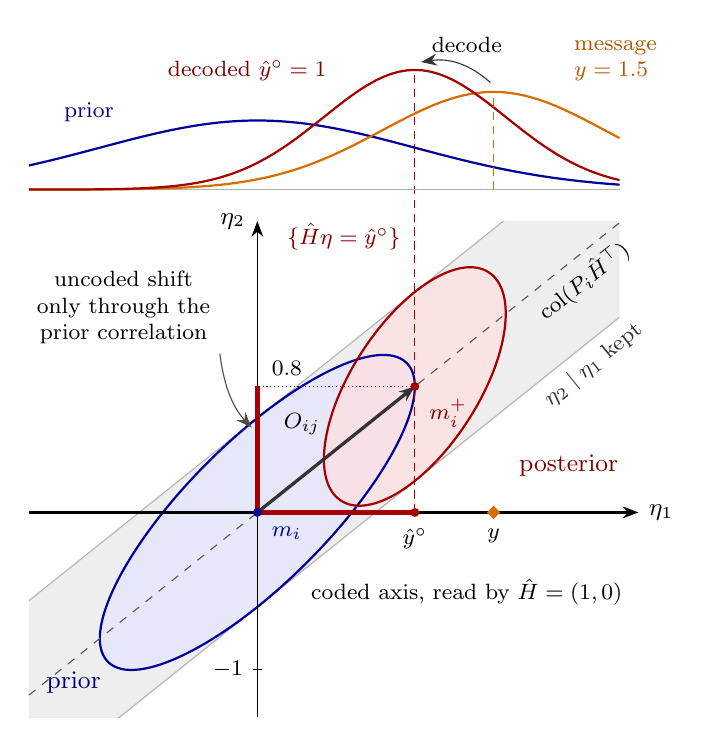
\begin{tikzpicture}[x=2cm, y=2cm, >={Stealth[length=2mm]}, every node/.style={font=\small}]
  % band: conditional law of eta_2 given eta_1, kept by the message
  \begin{scope}
    \clip (-1.45,-1.3) rectangle (2.3,1.85);
    \fill[gray!13] (-1.45,-1.76) -- (2.3,1.24) -- (2.3,2.44) -- (-1.45,-0.56) -- cycle;
    \draw[gray!60] (-1.45,-1.76) -- (2.3,1.24);
    \draw[gray!60] (-1.45,-0.56) -- (2.3,2.44);
  \end{scope}
  % prior and posterior one-standard-deviation ellipses
  \fill[blue!10, fill opacity=0.75, rotate around={45:(0,0)}] (0,0) ellipse [x radius=1.34164, y radius=0.44721];
  \fill[red!12, fill opacity=0.75, rotate around={57.1139:(1,0.8)}] (1,0.8) ellipse [x radius=0.86357, y radius=0.40114];
  \draw[blue!60!black, thick, rotate around={45:(0,0)}] (0,0) ellipse [x radius=1.34164, y radius=0.44721];
  \draw[red!65!black, thick, rotate around={57.1139:(1,0.8)}] (1,0.8) ellipse [x radius=0.86357, y radius=0.40114];
  % update direction col(P_i H^T) through m_i
  \draw[dashed, black!65] (-1.45,-1.16) -- (2.3,1.84) node[pos=1, anchor=north east, sloped, font=\footnotesize, black] {$\operatorname{col}(P_i\hat H^\top)$};
  % axes
  \draw[->, thick] (-1.45,0) -- (2.42,0) node[anchor=west] {$\eta_1$};
  \draw[->] (0,-1.3) -- (0,1.85) node[anchor=east, xshift=-1pt] {$\eta_2$};
  \draw (0.03,-1) -- (-0.03,-1) node[anchor=east, font=\footnotesize] {$-1$};
  \node[anchor=north east, font=\footnotesize] at (2.38,-0.36) {coded axis, read by $\hat H=(1,0)$};
  % fiber {H eta = decoded value}
  \draw[red!65!black, densely dashed] (1,0) -- (1,2.81);
  \node[anchor=east, font=\footnotesize, red!50!black] at (0.97,1.75) {$\{\hat H\eta=\hat y^\circ\}$};
  % coded and uncoded shifts
  \draw[red!65!black, line width=1.6pt] (0,0) -- (1,0);
  \draw[red!65!black, line width=1.6pt] (0,0) -- (0,0.8);
  \draw[red!65!black, densely dotted] (1,0.8) -- (0,0.8);
  \node[anchor=south west, font=\footnotesize] at (0.03,0.81) {$0.8$};
  \node[font=\footnotesize, align=center] (corr) at (-0.85,1.3) {uncoded shift\\only through the\\prior correlation};
  \draw[->, gray!60!black, shorten >=3pt] (corr.south east) to[bend right=18] (0,0.5);
  % lift
  \draw[->, very thick, black!80] (0,0) -- (1,0.8);
  \node[anchor=south east, font=\footnotesize] at (0.46,0.43) {$O_{ij}$};
  % means, message and decoded value on the coded axis
  \fill[blue!60!black] (0,0) circle (1.6pt);
  \node[anchor=north west, font=\footnotesize, blue!50!black] at (0.03,-0.03) {$m_i$};
  \fill[red!65!black] (1,0.8) circle (1.6pt);
  \node[anchor=north west, font=\footnotesize, red!50!black] at (1.03,0.78) {$m_i^+$};
  \fill[red!65!black] (1,0) circle (1.6pt);
  \node[anchor=north, font=\footnotesize] at (1,-0.04) {$\hat y^\circ$};
  \node[diamond, fill=orange!85!black, inner sep=0pt, minimum size=5pt] at (1.5,0) {};
  \node[anchor=north, font=\footnotesize] at (1.5,-0.04) {$y$};
  % labels of the ellipses
  \node[blue!50!black, anchor=north west] at (-1.4,-0.95) {prior};
  \node[red!50!black, anchor=west] at (1.6,0.3) {posterior};
  \path (0.75,0) -- (2.3,1.24) node[pos=0.84, anchor=north, sloped, font=\footnotesize, gray!40!black] {$\eta_2\mid\eta_1$ kept};
  % top strip: decode on the coded coordinate
  \draw[gray!60] (-1.45,2.05) -- (2.3,2.05);
  \draw[blue!60!black, thick] plot coordinates {(-1.45,2.2034) (-1.40,2.2147) (-1.35,2.2264) (-1.30,2.2385) (-1.25,2.2509) (-1.20,2.2636) (-1.15,2.2765) (-1.10,2.2896) (-1.05,2.3029) (-1.00,2.3162) (-0.95,2.3295) (-0.90,2.3427) (-0.85,2.3558) (-0.80,2.3687) (-0.75,2.3813) (-0.70,2.3935) (-0.65,2.4053) (-0.60,2.4165) (-0.55,2.4272) (-0.50,2.4373) (-0.45,2.4466) (-0.40,2.4551) (-0.35,2.4628) (-0.30,2.4695) (-0.25,2.4753) (-0.20,2.4801) (-0.15,2.4839) (-0.10,2.4866) (-0.05,2.4883) (0.00,2.4888) (0.05,2.4883) (0.10,2.4866) (0.15,2.4839) (0.20,2.4801) (0.25,2.4753) (0.30,2.4695) (0.35,2.4628) (0.40,2.4551) (0.45,2.4466) (0.50,2.4373) (0.55,2.4272) (0.60,2.4165) (0.65,2.4053) (0.70,2.3935) (0.75,2.3813) (0.80,2.3687) (0.85,2.3558) (0.90,2.3427) (0.95,2.3295) (1.00,2.3162) (1.05,2.3029) (1.10,2.2896) (1.15,2.2765) (1.20,2.2636) (1.25,2.2509) (1.30,2.2385) (1.35,2.2264) (1.40,2.2147) (1.45,2.2034) (1.50,2.1925) (1.55,2.1820) (1.60,2.1720) (1.65,2.1625) (1.70,2.1535) (1.75,2.1449) (1.80,2.1368) (1.85,2.1293) (1.90,2.1222) (1.95,2.1156) (2.00,2.1094) (2.05,2.1037) (2.10,2.0984) (2.15,2.0935) (2.20,2.0890) (2.25,2.0849) (2.30,2.0812)};
  \draw[orange!85!black, thick] plot coordinates {(-1.45,2.0501) (-1.40,2.0501) (-1.35,2.0502) (-1.30,2.0502) (-1.25,2.0503) (-1.20,2.0504) (-1.15,2.0506) (-1.10,2.0507) (-1.05,2.0509) (-1.00,2.0512) (-0.95,2.0515) (-0.90,2.0520) (-0.85,2.0525) (-0.80,2.0531) (-0.75,2.0539) (-0.70,2.0549) (-0.65,2.0561) (-0.60,2.0575) (-0.55,2.0593) (-0.50,2.0614) (-0.45,2.0638) (-0.40,2.0668) (-0.35,2.0703) (-0.30,2.0743) (-0.25,2.0790) (-0.20,2.0845) (-0.15,2.0908) (-0.10,2.0980) (-0.05,2.1062) (0.00,2.1154) (0.05,2.1258) (0.10,2.1374) (0.15,2.1503) (0.20,2.1645) (0.25,2.1801) (0.30,2.1970) (0.35,2.2154) (0.40,2.2351) (0.45,2.2561) (0.50,2.2783) (0.55,2.3017) (0.60,2.3261) (0.65,2.3513) (0.70,2.3772) (0.75,2.4036) (0.80,2.4302) (0.85,2.4568) (0.90,2.4830) (0.95,2.5086) (1.00,2.5333) (1.05,2.5568) (1.10,2.5788) (1.15,2.5991) (1.20,2.6172) (1.25,2.6330) (1.30,2.6463) (1.35,2.6568) (1.40,2.6644) (1.45,2.6691) (1.50,2.6706) (1.55,2.6691) (1.60,2.6644) (1.65,2.6568) (1.70,2.6463) (1.75,2.6330) (1.80,2.6172) (1.85,2.5991) (1.90,2.5788) (1.95,2.5568) (2.00,2.5333) (2.05,2.5086) (2.10,2.4830) (2.15,2.4568) (2.20,2.4302) (2.25,2.4036) (2.30,2.3772)};
  \draw[red!65!black, thick] plot coordinates {(-1.45,2.0501) (-1.40,2.0501) (-1.35,2.0502) (-1.30,2.0503) (-1.25,2.0504) (-1.20,2.0505) (-1.15,2.0507) (-1.10,2.0510) (-1.05,2.0514) (-1.00,2.0519) (-0.95,2.0525) (-0.90,2.0534) (-0.85,2.0545) (-0.80,2.0559) (-0.75,2.0577) (-0.70,2.0600) (-0.65,2.0628) (-0.60,2.0663) (-0.55,2.0707) (-0.50,2.0760) (-0.45,2.0824) (-0.40,2.0902) (-0.35,2.0994) (-0.30,2.1102) (-0.25,2.1229) (-0.20,2.1377) (-0.15,2.1546) (-0.10,2.1738) (-0.05,2.1954) (0.00,2.2196) (0.05,2.2463) (0.10,2.2755) (0.15,2.3072) (0.20,2.3410) (0.25,2.3769) (0.30,2.4145) (0.35,2.4533) (0.40,2.4929) (0.45,2.5328) (0.50,2.5724) (0.55,2.6110) (0.60,2.6479) (0.65,2.6825) (0.70,2.7141) (0.75,2.7421) (0.80,2.7658) (0.85,2.7849) (0.90,2.7988) (0.95,2.8072) (1.00,2.8101) (1.05,2.8072) (1.10,2.7988) (1.15,2.7849) (1.20,2.7658) (1.25,2.7421) (1.30,2.7141) (1.35,2.6825) (1.40,2.6479) (1.45,2.6110) (1.50,2.5724) (1.55,2.5328) (1.60,2.4929) (1.65,2.4533) (1.70,2.4145) (1.75,2.3769) (1.80,2.3410) (1.85,2.3072) (1.90,2.2755) (1.95,2.2463) (2.00,2.2196) (2.05,2.1954) (2.10,2.1738) (2.15,2.1546) (2.20,2.1377) (2.25,2.1229) (2.30,2.1102)};
  \draw[orange!85!black, densely dashed] (1.5,2.05) -- (1.5,2.67);
  \draw[->, black!80] (1.48,2.73) to[bend right=25] (1.04,2.86);
  \node[anchor=south, font=\footnotesize] at (1.33,2.86) {decode};
  \node[anchor=south east, font=\footnotesize, blue!50!black] at (-0.85,2.42) {prior};
  \node[anchor=south east, font=\footnotesize, red!50!black] at (0.5,2.68) {decoded $\hat y^\circ=1$};
  \node[anchor=south west, font=\footnotesize, orange!70!black, align=left] at (1.95,2.68) {message\\$y=1.5$};
\end{tikzpicture}

  \caption{\textbf{Decode, then lift.} A receiver with prior $\Ncal(m_i,P_i)$, $m_i=0$, unit variances and correlation $0.8$ reads the first coordinate of $\eta=(\eta_1,\eta_2)$ through the code $\hat H=(1,0)$ with noise variance $\hat R=0.5$, as receiver $i$ of \cref{ex:fw-disagreement} does at $\varrho=0.8$ and $\sigma^2=0.5$, and receives $y=1.5$. Top: on the coded coordinate its prior marginal (blue) and the likelihood of the message (orange) give a posterior marginal (red) whose mean is the decoded content $\hat y^\circ=1$, the message shrunk toward the prediction $\hat Hm_i=0$ by the factor $\hat HP_i\hat H^\top S^{-1}=2/3$ with $S=1.5$. Bottom: the receiver map $O_{ij}=(1,0.8)^\top$ lifts the decoded value along $\operatorname{col}(P_i\hat H^\top)$ to the posterior mean $m_i^+=(1,0.8)$, the receiver's own conditional mean on the line $\{\hat H\eta=\hat y^\circ\}$. The ellipses are one standard deviation of the prior (blue) and of the posterior (red), whose covariance is $P_i-P_i\hat H^\top\hat HP_i/1.5$. The gray band, the conditional mean $0.8\eta_1$ of $\eta_2$ given $\eta_1$ plus or minus one conditional standard deviation $0.6$, is left unchanged by the message, and both ellipses are tangent to its edges. The uncoded coordinate therefore moves by $0.8$ only through the prior correlation, and the functional $f^\top\eta=\eta_2-0.8\eta_1$, for which $f^\top P_i\hat H^\top=0$ (\cref{prop:fw-update-subspace}(c)), keeps its mean and its variance.}
  \label{fig:fw-lift}
\end{figure}

The author's second idea can now be stated exactly. Sender $j$'s map $T$ is its effective code $H_j$, which keeps the class of $m_j$ modulo $\ker H_j$. Receiver $i$'s map $O$ is the receiver map $O_{ij}$: among all beliefs consistent with a coded value it selects the one nearest to the receiver's prior mean in the receiver's own metric, which is also the receiver's prior conditional mean. On a noisy channel the receiver first decodes, shrinking the message toward its prediction, and the composite is the gain $\Kg$. When the code is read correctly and the channel is noiseless, the composition $O_{ij}H_j=\mathcal P_{ij}$ is a projector: the receiver adopts the sender's belief on the completed sent subspace $\operatorname{col}(P_iH_j^\top)$ and keeps its own along $\ker H_j$, the complement of that subspace orthogonal in the receiver's metric. The projection in the author's description is therefore $\mathcal P_{ij}$, a projection in the receiver's metric onto a subspace that the receiver's prior selects, so one message is projected differently by receivers with different priors. What the code does not carry is supplied by the receiver, and \eqref{eq:fw-meaning-lost} measures what is lost. Understanding is prior-dependent completion, which is one clause of hypothesis H2.

The lift uses the receiver's prior, so two receivers can read one message differently: with a common likelihood their gains agree exactly when their priors give the coded coordinates the same covariance with the whole state, and a message that both predict alike and find surprising can leave receivers with equal prior means further apart than before (Supplement, \cref{prop:fw-two-receivers,ex:fw-disagreement}).

\subsection{Interpretation levels and calibration classes}\label{sec:fw-levels}

A receiver must model how a message relates to the world. Hypothesis H2 says that receivers must model senders, and the structure of that model is the receiver's interpretation level. The levels differ in what they assume about the joint law of the message and the receiver's own information, which is where misreading enters (\cref{sec:mis}).

\begin{definition}[Interpretation levels]\label{def:fw-levels}
% src: L1-D3; decision 10 (law-header receivers are level 1)
Receiver $i$ reads a message $y_{ij}$ from sender $j$ with a code model $\hat H_{ij}$.
\begin{enumerate}
\item[] Level 0: $p^0_i(y_{ij}\mid\eta)=\Ncal(y_{ij};\hat H_{ij}\eta,\hat R_{ij})$. Messages are observations of $\eta$; $\hat R_{ij}=R_c$ by default, or a learned noise.
\item[] Level 1: $p^1_i(y_{ij}\mid\eta)=\Ncal(y_{ij};\hat H_{ij}\eta,\hat H_{ij}\hat P_{ij}\hat H_{ij}^\top+R_c)$. Messages are noisy estimates of $\eta$ whose errors are independent of everything the receiver knows and have covariance $\hat P_{ij}$, learned or read from a law header. In particular a receiver that reads a law header, adding the posted coded covariance $H_jP_jH_j^\top$ to the channel noise, reads at level 1, with $\hat H_{ij}\hat P_{ij}\hat H_{ij}^\top=H_jP_jH_j^\top$.
\item[] Exact fusion: $p^{\mathrm{ex}}_i(y_{ij}\mid\eta,\mathcal Z_i)$ is the conditional law of $y_{ij}$ given $(\eta,\mathcal Z_i)$ under the true joint process.
\end{enumerate}
\end{definition}

Levels 0 and 1 are conditionally independent of $\mathcal Z_i$ given $\eta$, and level 1 is level 0 with the noise $\hat R^1_{ij}=R_c+\hat H_{ij}\hat P_{ij}\hat H_{ij}^\top$ in place of $\hat R_{ij}$; we call both literal. In the Gaussian case exact fusion updates by Gaussian conditioning on $(\mathcal Z_i,y_{ij})$. In the track model, where $\mathcal Z_i=m_i$ and the errors $e_a=m_a-\eta$ are Gaussian and independent of $\eta$ with covariance blocks $\Sigma_{aa'}$,
\begin{equation}\label{eq:fw-track}
\begin{gathered}
y_{ij}\mid\eta,m_i\sim\Ncal\bigl(A_{ij}\eta+H_j\Sigma_{ji}\Sigma_{ii}^{-1}m_i,R^{\mathrm{ex}}_{ij}\bigr),\\
A_{ij}=H_j\bigl(I-\Sigma_{ji}\Sigma_{ii}^{-1}\bigr),\qquad R^{\mathrm{ex}}_{ij}=H_j\bigl(\Sigma_{jj}-\Sigma_{ji}\Sigma_{ii}^{-1}\Sigma_{ij}\bigr)H_j^\top+R_c,
\end{gathered}
\end{equation}
because given $(\eta,m_i)$ the receiver's error is known and $e_j\mid e_i\sim\Ncal(\Sigma_{ji}\Sigma_{ii}^{-1}e_i,\Sigma_{jj}-\Sigma_{ji}\Sigma_{ii}^{-1}\Sigma_{ij})$. The update with this likelihood is cross-covariance-aware track fusion \citep{barshalom1986effect}. Under a proper prior the error of a posterior mean is correlated with the state, and exact fusion must then use the full joint law.

\begin{proposition}[When each level is Bayes optimal]\label{prop:fw-level-optimality}
% src: L1-P1
Let $j$ send belief messages $y_{ij}=H_jm_j+\nu_{ij}$, and call a likelihood true when it is the conditional law of $y_{ij}$ given $(\eta,\mathcal Z_i)$ under the true joint process.
\begin{enumerate}
\item[(a)] Let the true conditional law have the density $p(y\mid\eta,\mathcal Z_i)$. A message likelihood $\hat p(y\mid\eta,\mathcal Z_i)$ yields the exact posterior, the one that combines the receiver's prior with $p$, if and only if, for $q_i$-almost every $\eta$, $\hat p(y\mid\eta,\mathcal Z_i)$ equals $p(y\mid\eta,\mathcal Z_i)$ times a positive factor that does not depend on $\eta$.
\item[(b)] The level-0 likelihood with $\hat R_{ij}=R_c$ is true if and only if $H_jm_j=\hat H_{ij}\eta$ almost surely, and level 0 is then exact: the coded content is exact, as for a public referent observed without noise. With a general $\hat R_{ij}$ it is true if and only if, given $(\eta,\mathcal Z_i)$, $H_jm_j\sim\Ncal(\hat H_{ij}\eta,\hat R_{ij}-R_c)$.
\item[(c)] The level-1 likelihood is true, and level 1 is then exact, if and only if the coded error $H_jm_j-\hat H_{ij}\eta$ is independent of $(\eta,\mathcal Z_i)$ with law $\Ncal(0,\hat H_{ij}\hat P_{ij}\hat H_{ij}^\top)$. Let the world be static, $\eta\sim\Ncal(\bar\eta,\Lambda_0^{-1})$ with $\Lambda_0\succ0$, observed through independent linear-Gaussian sources; let every agent hold the exact posterior given the sources it observes and $i$ retain its raw data; and let $\Lambda^{\mathrm{sh}}_{ij}$ be the precision that $i$ and $j$ share, the prior included. With $\hat H_{ij}=H_j$ and the header $\hat P_{ij}=P_j$, the level-1 likelihood is true if and only if $H_jP_j\Lambda^{\mathrm{sh}}_{ij}=0$, which fails for every nonzero code. Under a flat prior, $\Lambda_0=0$ with the precision of $j$'s sources positive definite and all laws taken conditionally on $\eta$, the same criterion $H_jP_j\Lambda^{\mathrm{sh}}_{ij}=0$ holds and nonzero codes can meet it; it is not implied by the absence of shared sources in the coded directions, $H_j\Lambda^{\mathrm{sh}}_{ij}=0$. Let $\Lambda_{j\setminus i}$ be the precision of the sources that $j$ observes and $i$ does not. If $\Lambda_{j\setminus i}\succ0$, the level-1 likelihood is true for an evidence message, which carries $\eta$ plus an error built only from those sources, read with the covariance of that error as its header.
\item[(d)] Exact fusion is exact relative to $\mathcal Z_i$, and it equals the posterior given all of $i$'s data when $\mathcal Z_i$ is sufficient for $(\eta,y_{ij})$ relative to those data.
\end{enumerate}
\end{proposition}

A proper common prior is itself shared information, so under it a posterior-mean message is never an evidence message, and level 1 needs the sender to know what the receiver lacks. Retaining only beliefs loses information: with prior, common-source and private precisions equal to one and a noiseless scalar message, a receiver that keeps its raw data gains $\tfrac12\ln(4/3)=0.144$ nats, one that keeps only its belief gains $\tfrac12\ln(11/9)=0.100$ nats, and a level-1 receiver believes it gains $\tfrac12\ln2=0.347$ nats (\cref{chk:fw-levels}). In a dynamic world the world's innovation is shared by every agent; in a scalar world this alone makes level 1 inexact for messages that carry the sender's filtered mean, even when the agents run steady-state Kalman filters on independent sensors (\cref{prop:mis-dynamic}). On trees the channel filter of decentralized fusion subtracts the information shared along each link \citep{grime1994data}; on graphs with cycles exact fusion needs provenance. Proof in \cref{app:fw}.

Calibration concerns the noise a literal receiver assigns to a message whose code model may be wrong, for instance because the receiver reads the sender through a wrong translation (\cref{def:fw-translation}).

\begin{definition}[Calibration classes]\label{def:fw-calibration}
% src: L3-D7, critic D5
A receiver $i$ reads $y_{ij}$ with code model $\hat H_{ij}$. Its calibration class says how it sets the noise $\hat R_{ij}$ of a level-0 likelihood or, in class $\mathsf{C2}$, the joint law of the message.
\begin{enumerate}
\item[] $\mathsf{C0}$: $\hat R_{ij}$ is fixed and does not respond to the actual reliability of the message.
\item[] $\mathsf{C1g}$ (grounded): $\hat R_{ij}$ is learned by maximum likelihood within the level-0 model on grounded rounds, on which the receiver observes the referent; its population value is the actual second moment of $y_{ij}-\hat H_{ij}\eta$.
\item[] $\mathsf{C1i}$ (innovation): $\hat R_{ij}$ is learned by matching the second moment of the innovations $y_{ij}-\hat H_{ij}m_i$ to the model's prediction $\hat H_{ij}P_i\hat H_{ij}^\top+\hat R_{ij}$.
\item[] $\mathsf{C2}$: the receiver's model of the joint law of the message, the world and its own information is correct on the subspace that grounded data identify.
\end{enumerate}
The classes map onto the levels as follows. $\mathsf{C0}$ is level 0 with fixed noise; $\mathsf{C1g}$ and $\mathsf{C1i}$ are level 0 with a learned marginal noise; level 1 is the receiver that adds a posted header to its noise; $\mathsf{C2}$ is exact fusion restricted to the identifiable subspace.
\end{definition}

The classes differ in what a receiver can notice. A $\mathsf{C0}$ receiver cannot register a mistranslation in its assigned precision, so its expected free energy is blind to it (\cref{prop:coh-c0-blind}). A $\mathsf{C1g}$ or $\mathsf{C1i}$ receiver converts mistranslation into message noise and can withdraw from a mistranslated sender (\cref{thm:coh-withdrawal}), although in the static two-group model of that theorem a $\mathsf{C1i}$ receiver registers mistranslation only in proportion to its own sensing gain. \Cref{tab:fw-levels} collects what each level needs.

\begin{table}[t]
\centering
\small
\begin{tabular}{@{}>{\raggedright\arraybackslash}p{1.8cm}>{\raggedright\arraybackslash}p{4.3cm}>{\raggedright\arraybackslash}p{5.2cm}>{\raggedright\arraybackslash}p{3.0cm}@{}}
\toprule
Level & Bayes optimal when & The receiver must know & Calibration class\\
\midrule
0 & the coded content is exact, or the message relays a fresh observation with the modeled noise & the sender's code, learned from grounded co-occurrence (\cref{sec:fw-learning}), and a noise model & $\mathsf{C0}$ (fixed noise); $\mathsf{C1g}$, $\mathsf{C1i}$ (learned noise)\\
1 & the coded error is independent of $(\eta,\mathcal Z_i)$: evidence messages, or a flat prior with $H_jP_j\Lambda^{\mathrm{sh}}_{ij}=0$ & in addition, the sender's error covariance, from a law header or learned & receivers that read a law header\\
Exact fusion & always, relative to $\mathcal Z_i$ & in addition, the joint law of the sender's information and its own: the cross-covariance in the track model, or the common information and the sender's information structure, which is provenance & $\mathsf{C2}$ on the identifiable subspace\\
\bottomrule
\end{tabular}
\caption{What each interpretation level needs (\cref{prop:fw-level-optimality}) and the calibration classes that realize it (\cref{def:fw-calibration}).}
\label{tab:fw-levels}
\end{table}

\subsection{Grounded learning of codes}\label{sec:fw-learning}

The code models $\hat H_{ij}$ used above have to come from somewhere. Because every generative model is about the same $\eta$, a receiver can learn a sender's code from the co-occurrence of messages with its own observations of the world, which is the formal content of grounding meaning in shared attention \citep{harnad1990symbol,tomasello2005understanding}. Here sender $j$'s messages are $y_t=H\phi_t+\nu_t$, with $H=H_j$, content $\phi_t\in\R^K$ in world coordinates (its belief, or a public component of $\eta$) and channel noise $\nu_t\sim\Ncal(0,R_c)$ independent of everything else. The receiver forms a regressor $\hat\phi_t$ from its own data $\mathcal Z_t$ without using $y_t$, and the pair is content calibrated if $\E[\phi_t\mid\mathcal Z_t]=\hat\phi_t$. Under exact joint attention both agents attend a public component of $\eta$, the sender knows it exactly and sends it, and the receiver's statistic is its posterior mean of that component. Write $M_2=\E[\hat\phi_t\hat\phi_t^\top]$ and $\mathcal P_M$ for the orthogonal projector onto $\operatorname{col}(M_2)$.

\begin{proposition}[Identification under content calibration]\label{prop:fw-grounded-identification}
% src: L1-P16
Let $(\phi_t,\hat\phi_t,\nu_t)$ be stationary and ergodic with finite second moments, and content calibrated.
\begin{enumerate}
\item[(a)] Every least-squares estimate satisfies $\hat H_TM_2\to HM_2$ almost surely, and the minimum-norm estimate converges to $H\mathcal P_M$.
\item[(b)] Under exact joint attention with an exactly observing receiver ($\hat\phi_t=\phi_t$), the joint law of $(\phi_t,y_t)$ depends on $H$ only through $H\mathcal P_M$: two codes are observationally equivalent if and only if they agree on $\operatorname{col}(\E[\phi_t\phi_t^\top])$.
\item[(c)] Let $\phi_t$ be centered Gaussian with second moment $M_\phi\succ0$, and let the receiver observe $\phi_t+v^g_t$, where the grounding noise $v^g_t\sim\Ncal(0,R^g)$, $R^g\succ0$, is independent of $\phi_t$ and of the channel, all jointly stationary and ergodic. Regressing $y_t$ on $\phi_t+v^g_t$ converges to the attenuated $HM_\phi(M_\phi+R^g)^{-1}$, while regressing on the calibrated statistic $M_\phi(M_\phi+R^g)^{-1}(\phi_t+v^g_t)$ converges to $H$.
\end{enumerate}
\end{proposition}

The unidentified directions are those along which the jointly attended content is identically zero (for centered content, those along which it never varies); on them the code never acts on that content, so misidentifying it there costs nothing for that content. Part (c) is regression dilution and its repair by regression calibration \citep{carroll2006measurement}. Proof in \cref{app:fw}; checked in \cref{chk:fw-learning}.

In the Supplement, under the hypotheses stated there, a recursive least-squares learner keeps its prior on the part of the code that acts off the column space of $M_2$ (\cref{prop:fw-rls}), and learning without content calibration converges to the regression of messages on the receiver's own beliefs, which differs from the grounded limit unless a moment condition holds (\cref{prop:fw-ungrounded-bias}).

\subsection{Direct, stigmergic and performative channels}\label{sec:fw-channels}

Messages are one of three ways in which an agent's actions reach another agent's senses. An agent can also write into a record that others read later, as termites build on earlier work \citep{grasse1959reconstruction,theraulaz1999brief,heylighen2016stigmergy}, and it can act on the world in a way that changes what the others' actions lead to, as a promise or a transfer does \citep{austin1962how}. \Cref{fig:fw-channels} shows the three paths. In the linear joint process let $X_t=(\eta_t,Y_t,Z_t)$ stack the world, the channel contents and the records, with dynamics $X_{t+1}=\bar FX_t+\sum_jB_ja_j(t)+\bar w_t$, $\bar F=\diag(F,0,F_z)$ and $B_j$ stacking $B^\eta_j$, $B^Y_j$, $B^Z_j$, and let agent $i$'s sensory states be $s_i(t)=H^X_iX_t+\bar v_i(t)$ with $H^X_i=(H^s_i,H^Y_i,H^Z_i)$ on a fixed attention schedule. The transfer kernel from $j$'s active states to $i$'s sensory states is $\mathcal X_{ij}(t,s)=\partial s_i(t)/\partial a_j(s)$ for $t>s$, computed with the other agents' actions held fixed.

\begin{proposition}[One transfer kernel]\label{prop:fw-transfer-kernel}
% src: L1-P20, L1-D12, L1-D13
\begin{equation}\label{eq:fw-kernel}
\mathcal X_{ij}(t,s)=H^Y_iB^Y_j\one[t-s=1]+H^Z_iF_z^{t-s-1}B^Z_j+H^s_iF^{t-s-1}B^\eta_j.
\end{equation}
The three terms are the direct, stigmergic and performative channels. Nilpotent modes carry direct messages, which need addressing and attention in the same round; passive persistent modes of the records, uncoupled from the world and entering no one's preferences, carry stigmergic communication; modes of the world carry performative acts. Reading has no back-action, since $H^X_i$ does not enter $\bar F$, so the information in a record is non-rival, whereas an act along a conserved direction $g$, with $g^\top F=g^\top$ and $g^\top B^\eta_j=0$ for every $j$, moves holdings between agents without creating them and is rival. Every channel type is a path $a_j\to X\to s_i$, so each agent's path blanket (\cref{def:col-blankets}) holds for all of them, from a start that the blanket screens.
\end{proposition}

Direct, stigmergic and performative communication are therefore one object with three kinds of modes, distinguished by latency, persistence and whether they move resources. Proof in \cref{app:fw}; checked in \cref{chk:fw-records}.

\begin{figure}[t]
  \centering
  \resizebox{\textwidth}{!}{% Figure: communication passes through external states (direct message, record, performative act).
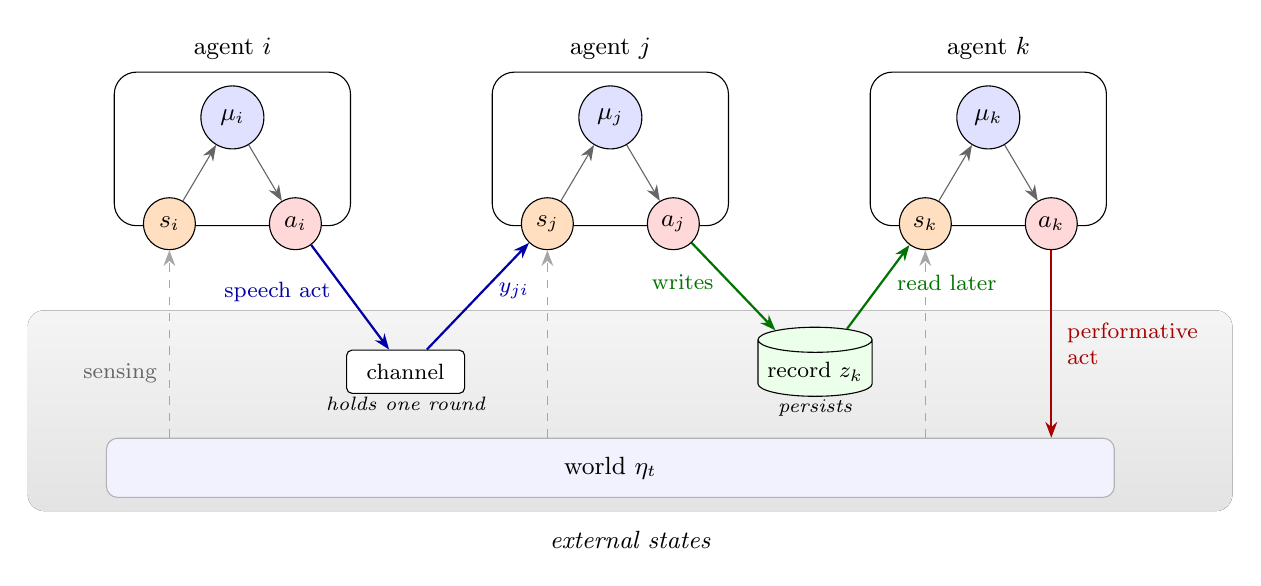
\begin{tikzpicture}[>={Stealth[length=2mm]}, every node/.style={font=\small},
    blank/.style={circle, draw, inner sep=0pt, minimum size=6.6mm},
    msg/.style={->, thick, blue!65!black},
    rec/.style={->, thick, green!45!black},
    perf/.style={->, thick, red!65!black},
    sens/.style={->, gray!70, dashed}]
  % external states
  \fill[rounded corners=6pt, top color=gray!8, bottom color=gray!22] (-0.4,-0.05) rectangle (14.9,2.5);
  \node[draw=gray!60, fill=blue!5, rounded corners=4pt, minimum width=12.8cm, minimum height=0.75cm] (eta) at (7,0.5) {world $\eta_t$};
  \node[draw, fill=white, rounded corners=2pt, minimum width=1.5cm, minimum height=0.55cm, font=\footnotesize] (chan) at (4.4,1.72) {channel};
  \node[draw, cylinder, shape border rotate=90, aspect=0.22, minimum width=1.45cm, minimum height=0.75cm, fill=green!8, font=\footnotesize] (rec) at (9.6,1.72) {record $z_k$};
  \node[below=0pt of chan, font=\scriptsize\itshape, inner sep=1pt] {holds one round};
  \node[below=0pt of rec, font=\scriptsize\itshape, inner sep=1pt] {persists};
  \node[font=\small\itshape] at (7.25,-0.42) {external states};
  % agents
  \foreach \nm/\x in {i/2.2, j/7.0, k/11.8} {
    \node[draw, rounded corners=8pt, minimum width=3.0cm, minimum height=1.95cm, fill=white] (A\nm) at (\x,4.55) {};
    \node[above=1pt of A\nm.north] {agent $\nm$};
    \node[blank, fill=blue!12, minimum size=8mm] (mu\nm) at (\x,4.95) {$\mu_\nm$};
    \node[blank, fill=orange!25] (s\nm) at ($(\x,3.6)+(-0.8,0)$) {$s_\nm$};
    \node[blank, fill=red!15] (a\nm) at ($(\x,3.6)+(0.8,0)$) {$a_\nm$};
    \draw[->, gray!80!black] (s\nm) -- (mu\nm);
    \draw[->, gray!80!black] (mu\nm) -- (a\nm);
    \draw[sens] (eta.north -| s\nm) -- (s\nm);
  }
  \node[left=1pt, font=\footnotesize, gray!80!black] at ($(eta.north -| si)!0.3!(si)$) {sensing};
  % direct message
  \draw[msg] (ai) -- node[pos=0.45, left=2pt, font=\footnotesize] {speech act} (chan);
  \draw[msg] (chan) -- node[pos=0.55, right=2pt, font=\footnotesize] {$y_{ji}$} (sj);
  % stigmergic record
  \draw[rec] (aj) -- node[pos=0.45, left=2pt, font=\footnotesize] {writes} (rec);
  \draw[rec] (rec) -- node[pos=0.55, right=2pt, font=\footnotesize] {read later} (sk);
  % performative act
  \draw[perf] (ak) -- node[pos=0.5, right=2pt, font=\footnotesize, align=left] {performative\\act} (eta.north -| ak);
\end{tikzpicture}
}
  \caption{\textbf{Communication passes through external states.} Each agent has sensory states $s$, internal states $\mu$ and active states $a$. A speech act of $i$ writes a message into a channel that holds it for one round, and $j$ reads it as $y_{ji}$ (blue). Agent $j$ writes a record $z_k$ that persists and that $k$ reads later (green). A performative act of $k$ changes the world state $\eta$ that every agent senses (red; sensing in gray). All three are paths from the active states of one agent through external states to the sensory states of another, so the agents' own blankets are respected.}
  \label{fig:fw-channels}
\end{figure}

Records persist, so they need a model of their own. We use one record model throughout, written for the world-conditional errors of the level-0 network of \cref{sec:fw-level0}.

\begin{definition}[Record model]\label{def:fw-record-model}
% src: B5-D1
Agents $i\in V$ sit at the sites $x_i$ of $\Z^D$ or at the vertices of a graph, and $e_i$ is the world-conditional error of agent $i$, the connected part of its error with the common mode of \cref{lem:fw-common-mode} removed. Records $z_{k,i}$, $k=1,\dots,n_z$, sit at the agents' sites. In rounds,
\begin{align}
e_i(t+1)&=\Bigl(1-\varepsilon'-\sum_k\beta_k\Bigr)e_i(t)+a\sum_{j\sim i}\bigl(e_j(t)-e_i(t)\bigr)+\sum_k\beta_k\sum_j\mathsf K_k(x_i-x_j)z_{k,j}(t)+\zeta_i(t),\label{eq:fw-record-agents}\\
z_{k,i}(t+1)&=\omega_ke_i(t)+(1-\omega_k-\delta_k)z_{k,i}(t)+\zeta^z_{k,i}(t),\label{eq:fw-record-records}
\end{align}
with message weight $a\ge0$ to each neighbor $j\sim i$, read weights $\beta_k$, write weights $\omega_k$, decays $\delta_k\ge0$, and read kernels $\mathsf K_k\ge0$ that sum to one; on $\Z^D$ the kernel $\mathsf K_k$ has second moment $\ell_{r,k}^2$ per coordinate, the reading range, and on a graph $\mathsf K_k(x_i-x_j)$ stands for a row-stochastic kernel $\mathsf K_k(i,j)$. The local noises $\zeta_i$, of variance $q>0$, and $\zeta^z_{k,i}$, of variance $q_z\ge0$, are independent across sites, records and rounds. The agents' leak after reading is
\begin{equation}\label{eq:fw-record-leak}
\varepsilon'=\varepsilon-\sum_k\upsilon_k\beta_k,
\end{equation}
where $\varepsilon$ is the leak without records (grounding, forgetting and turnover) and the displacement fraction $\upsilon_k\in[0,1]$ says what reading displaces: $\upsilon_k=0$ when it displaces only self-weight, so that the agents' row sums keep the value $1-\varepsilon$ they have without records, and $\upsilon_k=1$ when it displaces only leak.
\end{definition}

A record of a changing world holds a stale estimate, but its staleness and its decay toward a reference are functions of the world path, so given that path they shift the conditional mean and leave the conditional fluctuation, which this model describes, unchanged. Only exogenous variables are conditioned on: records written by agents remain part of the population, and in \cref{sec:col} their coordinates enter the world-conditional precision as nodes, a precision that record noise can make non-diffusive in computed cases (\cref{chk:sca-records-length}). In translation-invariant media the mean mode obeys a reduced model with one agent coordinate and one coordinate per record. \Cref{sec:sca} derives from it the effective leak, the exact condition under which a record lengthens memory and the correlation length with records (\cref{prop:sca-records,prop:sca-records-memory,prop:sca-records-length}), and \cref{sec:col} places records in the canonical partition (\cref{prop:col-records-partition}). The properties of a single record that do not depend on the network are stated in the Supplement (\cref{prop:fw-record-basics}).

These properties are its latency and mean delay, the delay to a first reading, its role as a hub between readers, and the write weight that maximizes its correlation with a scalar autoregressive world.

A performative act that is chosen independently of the present state, given the receiver's information, changes the world rather than the receiver's information about it; read as a level-0 message it moves the receiver's belief about the present state and omits the intervention, the confusion of intervention with observation (Supplement, \cref{prop:fw-performative}).

Attention, addressing and content are policies selected by expected free energy, worked out for linear-Gaussian slots in the Supplement (\cref{sec:fw-efe}). For an attention set, under the hypotheses stated there and up to an additive constant, it is minus the mutual information between the state and the attended messages, at levels 0 and 1 the believed value of \cref{def:mis-values}, plus a preference term and a constant per message (\cref{prop:fw-efe-communication}). For a sender, of the two preferences defined there, the preference to be understood is blind to agreement at correct code models, whereas the preference to be predicted, under the hypotheses stated there, selects partners whose believed coded disagreement is below a threshold (\cref{prop:fw-understood-predicted,prop:fw-bounded-confidence}); the fragmentation of such senders into belief clusters is conjectured and untested (\cref{conj:fw-fragmentation}).

\subsection{Frames}\label{sec:fw-frames}

A frame is the private coordinate system in which an agent stores its beliefs. In the linear case agent $i$ holds the internal mean $\mu_i=U_im_i$ and covariance $U_iP_iU_i^\top$ with $U_i\in\GL(K)$, and its internal model is the world model pushed forward by $U_i$: dynamics $U_iFU_i^{-1}$, sensing $H^s_iU_i^{-1}$ and innovation covariance $U_iQU_i^\top$. Frames are optional, and the results of this subsection say exactly what they change.

Inference is frame covariant: a redescription of an agent's frame, compensated in the code that the agent applies to its own internal coordinates, changes no message, no belief in world coordinates, no information quantity and no expected free energy, so frames have observable effects only through communication (Supplement, \cref{prop:fw-frame-covariance}).

A receiver can model a sender's code directly, or through a translation of the sender's internal coordinates into its own, which is how frames enter the models of \cref{sec:coh,sec:frm}.

\begin{definition}[Translations and mistranslation]\label{def:fw-translation}
% src: L3-D7, L1-P29, L7-P8; B2-D1 for translated full-rank messages
Receiver $i$ reads sender $j$'s internal coordinates through a translation $\Theta_{ij}\in\GL(K)$, learned or fixed, its model of the map from $j$'s internal coordinates to its own. The true translation is $U_iU_j^{-1}$. The mistranslation of the edge is the world-coordinate error
\begin{equation}\label{eq:fw-mistranslation}
\Upsilon_{ij}=U_i^{-1}\Theta_{ij}U_j,
\end{equation}
which is the identity exactly when the translation is true, and the translation induces the code model $\hat H_{ij}=T_c\Theta_{ij}^{-1}U_i=H_j\Upsilon_{ij}^{-1}$. When the public code is invertible ($r_c=K$), the receiver carries a message into world coordinates as $\tilde y_{ij}=U_i^{-1}\Theta_{ij}T_c^{-1}y_{ij}=\Upsilon_{ij}m_j+U_i^{-1}\Theta_{ij}T_c^{-1}\nu_{ij}$, and reading $\tilde y_{ij}$ as an observation of $\eta$ is reading $y_{ij}$ with the code model $\hat H_{ij}$.
\end{definition}

The identities follow by substitution: $H_j\Upsilon_{ij}^{-1}=T_cU_jU_j^{-1}\Theta_{ij}^{-1}U_i$, and $\tilde y_{ij}=\hat H_{ij}^{-1}y_{ij}$ when $r_c=K$. For planar frames and translations that are rotations the three matrices commute, and $\Upsilon_{ij}$ is the rotation by the angle of $\Theta_{ij}$ minus the angle of $U_iU_j^{-1}$, the translation error; these are the rotation errors of the two-group model of \cref{sec:frm}. True translations compose without holonomy, because intermediate encodings cancel around every cycle, as in $(U_iU_j^{-1})(U_jU_k^{-1})(U_kU_i^{-1})=I$, so a failure of consistency in the sense of \cref{sec:coh} comes from learned translations, from misspecified models or from agents of different kinds (\cref{prop:coh-flat-true}). Under noiseless reception the projectors $\mathcal P_{ij}$ of \cref{prop:fw-prior-completion}(d) compose around cycles of receivers; with heterogeneous prior covariances their product can amplify content, a calibration failure distinct from holonomy, which \cref{thm:coh-amplification} treats.

\begin{proposition}[Encodings enter only through effective codes]\label{prop:fw-effective-codes}
% src: L7-P1
With linear encodings, receivers at level 0, at level 1 or with exact fusion, known or learned code models, and attention and transmission selected by expected free energy, every message likelihood, reception update, true error recursion and expected-free-energy term depends on the encodings $(U_j)_{j\in V}$ only through the effective codes $H_j=T_cU_j$ and the receivers' models $\hat H_{ij}$ of them, or, for learned models, through the laws of those models. A receiver that knows $H_j$ can compute entirely in world coordinates, identity encodings give $H_j=T_c$ for every sender $j$ in modality $c$, and every configuration of frames with $H_j=T_c$ for every sender is indistinguishable from identity encodings in all of these quantities. When $r_c<K$ such configurations include non-identity frames, namely those with $T_c(U_j-I)=0$.
\end{proposition}

This extends to learned code models and exact fusion a statement for known codes in \citet{dennis2026communicating}. Consequently a result that holds with one common effective code per modality holds at identity encodings, and frames matter only where sender-specific effective codes do. Proof in \cref{app:fw}.

Frames are identifiable from messages only modulo the set $\{X:T_cX=0\}$, of dimension $K(K-r_c)$, and mismatches in that set cost nothing in reception (Supplement, \cref{prop:fw-frame-identifiability}); the cost of a misidentified code outside it is in \cref{prop:fw-misidentified-code}.

\subsection{The level-0 network and its common mode}\label{sec:fw-level0}

The scale theory, the definition of collectives and the formation model are built on one linear network, in which every receiver reads messages literally with fixed gains. In any network of agents that update from what they read, messages, record reads and performative acts enter an update as inputs from the agent's potential sources through external states, so influence travels along the potential communication graph; the general local rule, its influence bounds and routing by expected free energy are stated with the light cones of \cref{sec:sca} (\cref{thm:sca-lightcone,prop:sca-poisson,prop:sca-routing}). The quantitative results need the linear network, on which the light-cone, clustering and Ornstein--Zernike results of \citet{dennis2026communicating} were first obtained.

\begin{definition}[Level-0 network]\label{def:fw-level0}
% src: L3 Section 0.1, R1, B1-P1; L4-D1 to L4-D3 are stated in Section 8
Fix a time-invariant attention schedule. Agent $i$ holds a predicted mean $m_i(t)$ of $\eta_t$, formed at the end of round $t-1$, with prior error $e_i(t)=m_i(t)-\eta_t$. It senses $s_i(t)=H^s_i\eta_t+v_i(t)$ every round and reads from each attended sender $j$ the message $y_{ij}(t)=H_jm_j(t)+\nu_{ij}(t)$, with channel noise specific to the receiver. It fuses the messages literally, as observations of $\eta$, with time-invariant gains $\Kg^s_i$ and $\Kg_{ij}$ computed from its claimed covariances and assigned noises, so level-1 receivers, whose assigned noise includes a law header, are included:
\[
m_i^+(t)=m_i(t)+\Kg^s_i\bigl(s_i(t)-H^s_im_i(t)\bigr)+\sum_j\Kg_{ij}\bigl(y_{ij}(t)-\hat H_{ij}m_i(t)\bigr),\qquad m_i(t+1)=Fm_i^+(t).
\]
The stacked errors then obey
\begin{equation}\label{eq:fw-level0-error}
e(t+1)=We(t)+B^{\mathrm{mis}}\eta_t-\one\otimes w_t+\zeta(t),
\end{equation}
with blocks $W_{ii}=F\bigl(I-\Kg^s_iH^s_i-\sum_j\Kg_{ij}\hat H_{ij}\bigr)$, $W_{ij}=F\Kg_{ij}H_j$ for attended $j$ and $W_{ij}=0$ otherwise, mistranslation term $B^{\mathrm{mis}}_i=F\sum_j\Kg_{ij}(H_j-\hat H_{ij})$, and local noise $\zeta_i(t)=F\bigl(\Kg^s_iv_i(t)+\sum_j\Kg_{ij}\nu_{ij}(t)\bigr)$, independent across agents and rounds, with block-diagonal covariance $Q^\zeta$. In the scalar network write $k^s_i=\Kg^s_iH^s_i$ and $k_{ij}=\Kg_{ij}\hat H_{ij}$; then
\[
W_{ii}=F\Bigl(1-k^s_i-\sum_jk_{ij}\Bigr),\qquad W_{ij}=Fk_{ij}\frac{H_j}{\hat H_{ij}},\qquad B^{\mathrm{mis}}_i=F\sum_jk_{ij}\Bigl(\frac{H_j}{\hat H_{ij}}-1\Bigr),\qquad q_i=\Var(\zeta_i).
\]
The scalar $q_i$ is a noise variance, as are $q$ and $q_z$ in \cref{def:fw-record-model}; written with an argument or as a density, $q_i$ is the recognition density of agent $i$. With exact code models $B^{\mathrm{mis}}=0$, $W_{ij}=Fk_{ij}$, the row sums are $\lambda_i=F(1-k^s_i)$ and the local leak is $\varepsilon_i=1-\lambda_i=(1-F)+Fk^s_i$. In a homogeneous medium $a=Fk_{ij}$ is the message weight and $c=W_{ii}$ the self weight.
\end{definition}

The recursion \eqref{eq:fw-level0-error} follows from $e_i(t+1)=F(m_i^+(t)-\eta_t)-w_t$ by substituting $s_i=H^s_i(m_i-e_i)+v_i$ and $y_{ij}=H_j(\eta_t+e_j)+\nu_{ij}$. The leak is world decorrelation, which acts as forgetting, plus grounding through the sensing gain; a pure listener in a persistent world has no leak. When a receiver reads invertible codes through translations (\cref{def:fw-translation}) with isotropic gains $k_{ij}$ on the translated messages, $\Kg_{ij}=k_{ij}\hat H_{ij}^{-1}$, so $W_{ij}=Fk_{ij}\Upsilon_{ij}$ and $B^{\mathrm{mis}}_i=F\sum_jk_{ij}(\Upsilon_{ij}-I)$: a mistranslated message carries a transformed copy of the world. This is the error recursion of the two-group model of \cref{sec:frm}, applied round by round on a random schedule. Channel noise that a broadcast shares across its receivers is not local, and is treated like the world innovation below.

In the scalar network a literal receiver's gains $k^s_i$ and $k_{ij}$ are nonnegative and sum to less than one, so with exact code models and $F\ge0$ the matrix $W$ is entrywise nonnegative (Supplement, \cref{rem:fw-convex-gains}).

The world innovation enters every agent's error at once. The next lemma separates this common drive from the fluctuations that communication propagates.

\begin{lemma}[Common mode and connected part]\label{lem:fw-common-mode}
% src: L3-L1, B1-P1
In the level-0 network let $\rho(W)<1$, and let the world be stationary with $\rho(F)<1$ when $B^{\mathrm{mis}}\ne0$.
\begin{enumerate}
\item[(a)] The stationary error process is $e(t)=e^{\mathrm{com}}(t)+e^{\mathrm{loc}}(t)$ with
\begin{equation}\label{eq:fw-common-mode}
e^{\mathrm{com}}(t)=\sum_{n\ge0}W^n\bigl(B^{\mathrm{mis}}\eta_{t-1-n}-\one\otimes w_{t-1-n}\bigr),\qquad e^{\mathrm{loc}}(t)=\sum_{n\ge0}W^n\zeta(t-1-n),
\end{equation}
both series converging in mean square.
\item[(b)] The common part $e^{\mathrm{com}}$ is a measurable linear functional of the world path, the connected part $e^{\mathrm{loc}}$ is independent of the world path, and $\Cov(e)=\Cov(e^{\mathrm{com}})+\Sigma^{\mathrm{loc}}$, where $\Sigma^{\mathrm{loc}}=\sum_{n\ge0}W^nQ^\zeta(W^\top)^n$ is the unique solution of $\Sigma^{\mathrm{loc}}=W\Sigma^{\mathrm{loc}}W^\top+Q^\zeta$.
\item[(c)] If the local noises are Gaussian, then conditionally on the world path the error path is Gaussian, with conditional mean $e^{\mathrm{com}}$ and the law of $e^{\mathrm{loc}}$ around it; the conditional covariance $\Sigma^{\mathrm{loc}}$ does not depend on the path.
\item[(d)] In the scalar network with exact code models and equal sensing gains $k^s$, $W\one=\lambda\one$ with $\lambda=F(1-k^s)$, and $\Cov(e^{\mathrm{com}})=\frac{Q}{1-\lambda^2}\one\one^\top$, a pure common mode.
\end{enumerate}
\end{lemma}

The common mode does not decay with distance: it is the shared error of every echo chamber (\cref{thm:mis-echo-chambers}) and the accuracy side of the grounding tension (\cref{thm:coh-grounding-tension}). The connected part is what the clustering and Ornstein--Zernike results describe (\cref{thm:sca-clustering,thm:sca-oz}), and the conditional law given the world path, with broadcast noises shared by several receivers added to the conditioning set, is the object on which collectives are defined (\cref{def:col-world-conditional}). A mistranslated code adds a world-driven bias $B^{\mathrm{mis}}\eta_t$, which conditioning removes from the fluctuation but not from the error. Proof in \cref{app:fw}; checked in \cref{chk:fw-common-mode}.

\section{Misreading joint structure}\label{sec:mis}
% src: F_brief H2; C_critic V6; B_brief decision 6; L1 section 3; L3 sections 1 and 2

This section develops hypothesis H2: communication is an action, and receiving a message is a sensory process. In the author's formulation a sender projects its belief onto a subspace through a map $T$ and a receiver lifts the message into its full belief space through a map $O$ (\cref{sec:fw-codes,sec:fw-reception}). A receiver that treats a message as sensing must model how it was generated, and a message is generated from the sender's belief, which is a function of the sender's information and of its prior. That information overlaps with the receiver's through the common prior, through shared sources and, in a changing world, through the world's own innovations, and the sender's prior shapes the content in directions the sender never observed. A literal receiver reads the message as a measurement of the coded coordinates of $\eta$ and so misreads this joint structure in both directions. It overvalues a message whose error is redundant with its own, which is double counting, and it undervalues a message whose error complements its own, whose shared part it could subtract, or whose content completes a coordinate it already knows. We state the scope of each direction and then follow misreading from single messages to groups: in every group closed under attention the shared error has a floor that no statistic of the members' agreement reveals, and with homogeneous grounding and reversible weights such groups are echo chambers. Exact fusion, which reads messages under the true joint law and needs provenance, is the calibrated reference.

Indices are receiver first: $y_{ij}=H_jm_j+\nu$ is the message received by $i$ from $j$, $H_j=T_cU_j$ is the sender's effective code, $\nu\sim\Ncal(0,R_c)$, and $\hat H_{ij}$ is the receiver's model of the code. Among the interpretation levels of \cref{def:fw-levels}, level 0 models $y_{ij}\mid\eta\sim\Ncal(\hat H_{ij}\eta,\hat R_{ij})$ with $\hat R_{ij}=R_c$ unless stated (class $\mathsf{C0}$ of \cref{def:fw-calibration}); level 1 uses the noise $\hat R^1_{ij}=R_c+\hat H_{ij}\hat P_{ij}\hat H_{ij}^\top$, where $\hat P_{ij}$ is the sender's error covariance as the receiver knows it, from a law header posted with the message or from a learned confidence, so that a receiver that reads law headers is a level-1 receiver; and exact fusion uses the law of $y_{ij}$ given $\eta$ and everything the receiver retains, under the true joint process. We call levels 0 and 1 literal: both treat a message as conditionally independent of the receiver's information given $\eta$, and \cref{prop:fw-level-optimality} characterizes when that is exact.

\subsection{Believed and true value of a message}\label{sec:mis-values}

Misreading is measured by the gap between the information a receiver believes a message carries, which enters its expected free energy of attention, and the information the message carries.

\begin{definition}[Believed and true value]\label{def:mis-values}
Let receiver $i$ retain the information $\mathcal Z_i$ when messages arrive (its raw data, or only its belief statistics), so that its prior is $p(\eta\mid\mathcal Z_i)$. For a set $\mathcal J$ of attended senders with messages $y_{i\mathcal J}=(y_{ij})_{j\in\mathcal J}$, the \emph{believed values} $\mathcal V^0_i(\mathcal J)$ and $\mathcal V^1_i(\mathcal J)$ are the mutual informations of $\eta$ and $y_{i\mathcal J}$ under $i$'s level-0 and level-1 models with this prior, and the \emph{true value} is $\mathcal V^\ast_i(\mathcal J)=I(\eta;y_{i\mathcal J}\mid\mathcal Z_i)$ under the true joint process. The receiver \emph{overvalues} $\mathcal J$ at a level if its believed value at that level exceeds $\mathcal V^\ast_i(\mathcal J)$, and \emph{undervalues} it if its believed value is smaller. A level-0 model with $\hat R_{ij}=R_c=0$ treats the coded coordinates as observed exactly, and we then read $\mathcal V^0_i=+\infty$.
\end{definition}
% src: L1-D4

The believed value is the expected information of an experiment \citep{lindley1956measure} and the epistemic term of the expected free energy of attention (\cref{prop:fw-efe-communication}; \citealp{friston2015epistemic}). The true value is the believed value of an exact-fusion receiver.

Under a Gaussian prior, and where the noise that a level assigns to each message is positive definite, both believed values are log-determinants that depend on a sender only through its code, noise and posted confidence, never through the cross-covariance of the two agents' errors, and they are monotone and submodular in the set of senders (Supplement, \cref{prop:mis-believed-values}). The true value is not submodular: two senders with anticorrelated errors can be worth more together than the sum of their separate values (Supplement, \cref{ex:mis-nonsubmodular}).

A belief message is an observation of $\eta$ through the attenuated code $B_j=H_j(I-P_jP_0^{-1})$, where $P_0$ is the prior covariance and $P_j$ the sender's posterior covariance, with noise that includes the sender's estimation noise; level 0 omits both, and level 1 enlarges the noise but keeps the unattenuated code (Supplement, \cref{lem:mis-attenuation}).

\begin{definition}[Static common-source world]\label{def:mis-common-source}
The world is static with a proper common prior, $\eta\sim\Ncal(\bar\eta,P_0)$ and $\Lambda_0=P_0^{-1}\succ0$. Independent sources $o_u=H^s_u\eta+v_u$, $v_u\sim\Ncal(0,R^s_u)$, $u\in\mathcal U$, contribute the precisions $\Gamma_u=(H^s_u)^\top(R^s_u)^{-1}H^s_u$. Agent $k$ observes the sources in $\mathcal U_k\subseteq\mathcal U$ and holds the exact posterior $\Ncal(m_k,P_k)$, $\Lambda_k=P_k^{-1}=\Lambda_0+\sum_{u\in\mathcal U_k}\Gamma_u$. For a receiver $i$ and a sender $j$ the \emph{shared precision} is $\Lambda^{\mathrm{sh}}_{ij}=\Lambda_0+\sum_{u\in\mathcal U_i\cap\mathcal U_j}\Gamma_u$ and the sender's \emph{private precision} is $\Lambda_{j\setminus i}=\sum_{u\in\mathcal U_j\setminus\mathcal U_i}\Gamma_u$, so $\Lambda_j=\Lambda^{\mathrm{sh}}_{ij}+\Lambda_{j\setminus i}$. Unless stated otherwise the receiver retains its raw data, $\mathcal Z_i=\sigma(o_u:u\in\mathcal U_i)$, models the code correctly, $\hat H_{ij}=H_j$, and at level 1 reads the header $\hat P_{ij}=P_j$.
\end{definition}
% src: L1-D6

\begin{lemma}[Errors and the true value]\label{lem:mis-common-source}
In the static common-source world let $e_k=m_k-\eta$.
\begin{enumerate}
\item[(a)] $\Var(e_k)=P_k$, $\Cov(e_i,e_j)=P_i\Lambda^{\mathrm{sh}}_{ij}P_j$ and $\Cov(e_k,\eta)=-P_k$. In the symmetric scalar configuration, with prior precision $\Lambda_0$, one common source of precision $\Gamma_{\mathrm{com}}$ and one private source of precision $\Gamma_{\mathrm{pr}}$ for each agent, the error correlation is the shared fraction of precision $\phi=(\Lambda_0+\Gamma_{\mathrm{com}})/(\Lambda_0+\Gamma_{\mathrm{com}}+\Gamma_{\mathrm{pr}})$.
\item[(b)] Let $A_{ij}=H_jP_j\Lambda_{j\setminus i}$ and $R^{\mathrm{ex}}_{ij}=H_jP_j\Lambda_{j\setminus i}P_jH_j^\top+R_c$, and suppose $R^{\mathrm{ex}}_{ij}\succ0$, as it is when $R_c\succ0$. Then
\begin{equation}\label{eq:mis-true-value}
\mathcal V^\ast_i(\{j\})=\tfrac12\ln\det\bigl(I+(R^{\mathrm{ex}}_{ij})^{-1}A_{ij}P_iA_{ij}^\top\bigr).
\end{equation}
\item[(c)] If $H_j$ is invertible and $R_c=0$, the exact posterior has precision $\Lambda_i+\Lambda_j-\Lambda^{\mathrm{sh}}_{ij}$ and information vector $\Lambda_im_i+\Lambda_jm_j-\Lambda_0\bar\eta-h^{\mathrm{sh}}_{ij}$, with $h^{\mathrm{sh}}_{ij}=\sum_{u\in\mathcal U_i\cap\mathcal U_j}(H^s_u)^\top(R^s_u)^{-1}o_u$; the common information is subtracted once, and $\mathcal V^\ast_i(\{j\})=\tfrac12\ln\det(I+P_i\Lambda_{j\setminus i})$.
\item[(d)] Under the hypothesis of (b), exact fusion moves the mean within $\operatorname{col}(P_i\Lambda_{j\setminus i}P_jH_j^\top)$, whereas literal receivers move it within $\operatorname{col}(P_iH_j^\top)$ (\cref{prop:fw-update-subspace}).
\end{enumerate}
\end{lemma}
% src: L1-P7, L1-P8

Proof in \cref{app:mis}. Exact fusion reads the message through $A_{ij}$, which keeps only the part of the content that comes from information the receiver lacks; for a receiver that knows only the prior, $A_{ij}$ is the attenuated code $B_j$. Computing it requires $P_j$, $\Lambda_{j\setminus i}$ and the shared information vector, that is, knowledge of which of its sources the sender also used. We call this requirement provenance and return to it in \cref{sec:mis-exact}. The closed forms are checked against exact conditioning in \cref{chk:mis-values}.

\subsection{Overvaluation and its scope}\label{sec:mis-over}

Double counting is the familiar form of misreading. In the scalar track model, in which the two estimates have jointly Gaussian errors independent of $\eta$ with covariance $\sigma_{ij}$, level 1 with the sender's error variance as header overvalues a message exactly when $0<\sigma_{ij}<\sigma_{\mathrm b}$, a band of positive covariances whose upper edge $\sigma_{\mathrm b}$ is given in \eqref{eq:mis-band}, and undervalues it for negative covariance and above the band (Supplement, \cref{prop:mis-track-band}). In the common-source world the scope depends on codes, noise and the distribution of information.

\begin{proposition}[Scope of overvaluation]\label{prop:mis-overvaluation-scope}
In the static common-source world, with level-0 noise $\hat R_{ij}=R_c$:
\begin{enumerate}
\item[(a)] $\mathcal V^0_i\ge\mathcal V^1_i$ for every code and noise;
\item[(b)] in a scalar world ($K=1$), $\mathcal V^\ast_i<\mathcal V^1_i$ for every nonzero code gain and every $R_c\ge0$, and in the flat-prior limit equality holds exactly when the agents share no source;
\item[(c)] if $H_j$ is invertible and $R_c=0$, then $\mathcal V^\ast_i=\tfrac12\ln\det(I+P_i\Lambda_{j\setminus i})<\tfrac12\ln\det(I+P_i\Lambda_j)=\mathcal V^1_i$;
\item[(d)] in aligned worlds, where $\Lambda_0$ and every $\Gamma_u$ are diagonal in one basis, the rows of $H_j$ are multiples of distinct basis vectors and $R_c$ is diagonal, $\mathcal V^\ast_i\le\mathcal V^1_i\le\mathcal V^0_i$;
\item[(e)] if $\mathcal U_i\subseteq\mathcal U_j$ and $R_c\succ0$, then $\mathcal V^\ast_i\le\mathcal V^0_i$ for every code.
\end{enumerate}
\end{proposition}
% src: L1-P10

Proof in \cref{app:mis}. Part (e) fails at level 1 (\cref{ex:mis-cancellation}) and part (c) fails with channel noise (\cref{obs:mis-random-codes}); parts (b) to (e) are tested on random instances in \cref{chk:mis-values,chk:mis-scope}. The classical form of double counting is the overconfidence that overvaluation produces.

With an invertible code and no channel noise, a level-1 receiver adopts the precision $\Lambda_i+\Lambda_j$, which counts $\Lambda^{\mathrm{sh}}_{ij}$ twice, and its actual mean-square error exceeds the covariance it claims (Supplement, \cref{prop:mis-level1-mse}). Repeating the exchange over a graph compounds the excess (\cref{prop:agy-literal-consensus}), and the same overvaluation arises across the levels of a hierarchy (\cref{prop:hie-literal-once,prop:hie-literal-records}).

\begin{proposition}[Closed-form ratios and repetition]\label{prop:mis-closed-ratios}
In a scalar static common-source world let the code gain be $g\neq0$ and the channel noise $R_c\ge0$. In the symmetric scalar configuration put $P=(\Lambda_0+\Gamma_{\mathrm{com}}+\Gamma_{\mathrm{pr}})^{-1}$ and let $\varrho_c=R_c/(g^2P)$ be the noise-to-signal ratio.
\begin{enumerate}
\item[(a)] For a receiver that retains its raw data,
\begin{equation}\label{eq:mis-ratios}
\mathcal V^\ast_i=\tfrac12\ln\Bigl(1+\frac{(1-\phi)^2}{1-\phi+\varrho_c}\Bigr),\qquad\mathcal V^1_i=\tfrac12\ln\Bigl(1+\frac1{1+\varrho_c}\Bigr),\qquad\mathcal V^0_i=\tfrac12\ln\Bigl(1+\frac1{\varrho_c}\Bigr).
\end{equation}
As $\phi\uparrow1$ with $\varrho_c>0$, $\mathcal V^\ast_i=(1-\phi)^2/(2\varrho_c)+O((1-\phi)^3)$, so both $\mathcal V^1_i/\mathcal V^\ast_i$ and $\mathcal V^0_i/\mathcal V^\ast_i$ diverge like $(1-\phi)^{-2}$; at $\varrho_c=0$, $\mathcal V^1_i/\mathcal V^\ast_i=\ln2/\ln(2-\phi)$.
\item[(b)] For a receiver that retains only $m_i$, in the flat-prior limit, $\mathcal V^\ast_i=\tfrac12\ln\bigl((2(1-\phi)+\varrho_c)/(1-\phi^2+\varrho_c)\bigr)$, which tends to $0$ as $\phi\to1$.
\item[(c)] Let $n_{\mathrm r}$ relays observe the same sources, so that they hold one posterior $\Ncal(m_r,P_r)$, let their private precision relative to the receiver be $\Gamma_{\mathrm{rel}}>0$, and let each send $m_r$ with unit code through an independent channel of noise $R_c>0$. Then $\mathcal V^\ast_i=\tfrac12\ln\bigl(1+P_i/(\Gamma_{\mathrm{rel}}^{-1}+R_c/(n_{\mathrm r}P_r^2\Gamma_{\mathrm{rel}}^2))\bigr)$ increases to $\tfrac12\ln(1+P_i\Gamma_{\mathrm{rel}})$, while $\mathcal V^1_i=\tfrac12\ln(1+n_{\mathrm r}P_i/(P_r+R_c))$ grows like $\tfrac12\ln n_{\mathrm r}$.
\end{enumerate}
\end{proposition}
% src: L1-P11

Proof in \cref{app:mis}. Level 1's believed value does not depend on $\phi$ at all; at $\varrho_c=0.5$ the ratio $\mathcal V^1_i/\mathcal V^\ast_i$ is $2.29$, $30.9$ and $2605$ at $\phi=0.5$, $0.9$ and $0.99$ (\cref{chk:mis-ratios}). Part (c) is the persuasion bias of \citet{demarzo2003persuasion}, a failure to account for repetition. \citet{eyster2010naive} show that agents who neglect that others' actions embed earlier signals become confident even when wrong, and \citet{enke2019correlation} find experimentally that many people neglect correlation between signals.

In a dynamic world the world's innovation is a source every agent shares. In a scalar world with process noise the steady-state filtered errors of two agents with independent sensors are positively correlated, so a level-1 receiver of a filtered mean is overconfident, and a receiver of predictive means with law headers claims an innovation covariance that differs from the actual one by an explicit identity (Supplement, \cref{prop:mis-dynamic}).

\subsection{Undervaluation}\label{sec:mis-under}

Literal receivers also undervalue, through three mechanisms. Complementary errors are the first (\cref{prop:mis-track-band,ex:mis-nonsubmodular}); the other two need rank-limited or noisy codes.

The second is common-information cancellation: when a code mixes a coordinate on which the sender's information is shared with one on which it is private, the exact receiver subtracts the shared part, and in a closed-form example level 1 undervalues the message when the shared precision on the private coordinate is small (Supplement, \cref{ex:mis-cancellation}). The third is sender-side completion: the message carries the sender's prior completion of a coordinate the receiver already knows, and in the limit of precise observations the ratio of true to believed value is unbounded (Supplement, \cref{ex:mis-sender-completion}).

A numerical observation on random static common-source worlds finds undervaluation at both levels, with invertible noisy codes and with rank-limited codes, in the ensembles and with the seed stated there (Supplement, \cref{obs:mis-random-codes}).

\begin{table}[t]
\centering\small
\caption{When literal receivers overvalue and when they can undervalue. ``Over'' means that the believed value is at least the true value throughout the setting, ``under'' that it is below the true value throughout, and ``can be under'' that some instances are undervalued. Level-0 entries for the track model assume channel noise $R_c>0$.}\label{tab:mis-scope}
\begin{tabular}{@{}>{\raggedright\arraybackslash}p{0.35\textwidth}>{\raggedright\arraybackslash}p{0.12\textwidth}>{\raggedright\arraybackslash}p{0.17\textwidth}>{\raggedright\arraybackslash}p{0.26\textwidth}@{}}
\toprule
Setting & Level 1 & Level 0 & Result\\
\midrule
Track model, $0<\sigma_{ij}<\sigma_{\mathrm b}$ & over & over & \cref{prop:mis-track-band}\\
Track model, complementary errors ($\sigma_{ij}<0$) & under & under near $-\sigma_i\sigma_j$ & \cref{prop:mis-track-band}\\
Track model, $\sigma_{\mathrm b}<\sigma_{ij}<\sigma_i\sigma_j$ & under & under near $\sigma_i\sigma_j$ if $\sigma_j>2\sigma_i$ & \cref{prop:mis-track-band}\\
Scalar world & over & over & \cref{prop:mis-overvaluation-scope}(a, b)\\
Invertible noiseless code & over & over & \cref{prop:mis-overvaluation-scope}(a, c)\\
Aligned world & over & over & \cref{prop:mis-overvaluation-scope}(d)\\
Receiver's sources among the sender's & can be under & over & \cref{prop:mis-overvaluation-scope}(e), \cref{ex:mis-cancellation}\\
Sender completes a coordinate the receiver knows & under & under & \cref{ex:mis-sender-completion}\\
Rank-limited or noisy codes in general & can be under & can be under & \cref{obs:mis-random-codes}\\
\bottomrule
\end{tabular}
\end{table}

Both directions have one cause: a literal receiver reads a message as a measurement of coded coordinates, whereas a message is a function of the sender's information shaped by its prior (\cref{lem:mis-attenuation}). Redundancy lowers a message's value; the predictability of its shared part, complementary errors and the sender's completion raise it. Where only redundancy can act, literal receivers overvalue; elsewhere they can undervalue without bound (\cref{tab:mis-scope}). We therefore state hypothesis H2 as misreading of joint structure, with double counting as its overvaluation case.

\subsection{Social innovations are blind to shared error}\label{sec:mis-blind}

When messages circulate, misreading becomes a property of groups, and the error the members share is what is at stake. We study groups in the scalar level-0 network of \cref{def:fw-level0}. The world is $\eta_{t+1}=F\eta_t+w_t$ with $F\ge0$; agent $i$ holds a predicted mean $m_i(t)$ of $\eta_t$, senses $s_i(t)=\eta_t+v_i(t)$, reads $y_{ij}(t)=m_j(t)+\nu_{ij}(t)$ from the senders it attends, updates with the sensing gain $k^s_i$ and message gains $k_{ij}$, $k^s_i+\sum_jk_{ij}\le1$, and predicts with $F$. The errors $e_i(t)=m_i(t)-\eta_t$ obey
\begin{equation}\label{eq:mis-level0}
e(t+1)=We(t)+\zeta(t)-w_t\one,\qquad W_{ii}=F\Bigl(1-k^s_i-\sum_jk_{ij}\Bigr),\quad W_{ij}=Fk_{ij},
\end{equation}
with local noise $\zeta_i(t)=F(k^s_iv_i(t)+\sum_jk_{ij}\nu_{ij}(t))$ of variance $q_i$, independent across agents and rounds. The recursion uses only that receivers fuse linearly with fixed gains, so it covers level-1 receivers whose headers have reached their stationary values as well as level-0 receivers. The matrix $W$ is nonnegative with row sums $F(1-k^s_i)$, and for time-invariant $W$ with $\rho(W)<1$ the stationary error is the sum of two independent parts (\cref{lem:fw-common-mode}), the common mode $e^{\mathrm{com}}(t)=-\sum_{s\ge0}w_{t-1-s}W^s\one$ and the local part $e^{\mathrm{loc}}(t)=\sum_{s\ge0}W^s\zeta(t-1-s)$.

\begin{lemma}[Social innovations are blind to shared error]\label{lem:mis-social-blind}
Let receivers read messages with correct code models, and add an arbitrary process $x(t)$ to every agent's error, $e_i(t)\mapsto e_i(t)+x(t)$. Every social innovation $y_{ij}(t)-m_i(t)=e_j(t)-e_i(t)+\nu_{ij}(t)$ is unchanged, while every sensory innovation $s_i(t)-m_i(t)=v_i(t)-e_i(t)$ shifts by $-x(t)$. Every statistic of social innovations alone is therefore unchanged by a shared error, and only sensory innovations carry information about it.
\end{lemma}
\begin{proof}
Substitute $m_k=\eta+e_k$ into the two innovations. For a general effective code read correctly, the social innovation is $y_{ij}-H_jm_i=H_j(e_j-e_i)+\nu$, which is unchanged as well.
\end{proof}
% src: L3-L2

A precision learned from agreement therefore certifies mutual predictability, not accuracy, and a group with a large common error looks calibrated from inside. A record that the members write and read is blind in the same way (\cref{lem:hie-record-blind}); the cases of receivers of class $\mathsf{C1i}$ and of receivers that read law headers are in the Supplement (\cref{sup:mis-blindness-to-shared-error}).

\subsection{Echo chambers}\label{sec:mis-echo}

Closed groups of literal receivers can agree closely while sharing a large error about the world. We define this condition and show that closure under attention produces it when grounding is homogeneous and the weights are reversible.

\begin{definition}[Echo chamber]\label{def:mis-echo}
Fix a set $C$ of agents with stationary beliefs and a positive-definite weight $\Psi$ on $\R^K$ (for example $P_0^{-1}$), and write $\lVert x\rVert_\Psi^2=x^\top\Psi x$. The internal disagreement and the inaccuracy of $C$ are
\begin{equation}\label{eq:mis-echo}
\mathcal D_C=\max_{i,j\in C}\E\lVert m_i-m_j\rVert_\Psi^2,\qquad\mathcal A_C=\min_{i\in C}\E\lVert m_i-\eta\rVert_\Psi^2,
\end{equation}
and $\mathcal A_C/\mathcal D_C$ is its echo ratio. The set $C$ is an $(\alpha_{\mathcal D},\alpha_{\mathcal A})$-echo chamber if $\mathcal D_C\le\alpha_{\mathcal D}$ and $\mathcal A_C\ge\alpha_{\mathcal A}$. It is \emph{weak} if in addition $\mathcal A_C>\mathcal A^{\mathrm{iso}}_C$, the smallest error a member would have from its own sensory stream under exact inference, so that communication left even the best-informed member worse off; \emph{strong} if $\mathcal A_C\ge\tr(\Psi P_0)$, so that no member knows more about the current state than the prior; and \emph{self-sealed} if every member is overconfident: its claimed covariance lies below its actual mean-square-error matrix in the Loewner order and differs from it. A set is \emph{closed under attention}, an epistemic bubble, if no member attends a non-member.
\end{definition}
% src: L3-D3

Small disagreement means mutually predictable beliefs; the relation to the epistemic bubbles and echo chambers of \citet{nguyen2020echo} is in the Supplement (\cref{sup:mis-echo-chambers-in-the-literature}).

\begin{proposition}[Mean-square floor]\label{prop:mis-mse-floor}
In a stationary network \eqref{eq:mis-level0} with time-invariant $W$, $F\ge0$ and $\rho(W)<1$, every agent's mean-square error satisfies
\begin{equation}\label{eq:mis-floor}
\E e_i^2\ge\frac{Q}{1-F^2(1-k^s_{\max})^2},\qquad k^s_{\max}=\max_jk^s_j.
\end{equation}
If a set $C$ is closed under attention and $\rho(W_{CC})<1$, which $\rho(W)<1$ implies, the bound holds for its members with $k^s_{\max}$ taken over $C$; a closed set of pure listeners ($k^s_i=0$ for $i\in C$) has mean-square error at least $Q/(1-F^2)=P_0$.
\end{proposition}
% src: L3-P6

Proof in \cref{app:mis}. When the members of a closed set with a common sensing gain also read a record written from their own predicted means, the floor factor is at least that of \eqref{eq:mis-floor}, strictly when they sense, and nondecreasing in the weight they give the record (\cref{thm:hie-floor}). The disagreement side is bounded by a noise-to-gap ratio.

\begin{lemma}[Disagreement bound]\label{lem:mis-disagreement}
Let $C$ be closed under attention with a common sensing gain $k^s$, so that $W_{CC}=F(1-k^s)M$ with $M$ row-stochastic, and let $M$ be reversible with respect to a positive probability vector $\varpi$, $\varpi_iM_{ij}=\varpi_jM_{ji}$. Let $\sigma_\ast$ be the spectral radius of $M$ on $\{x:\varpi^\top x=0\}$, $\varpi_{\min}=\min_{i\in C}\varpi_i$ and $\bar q_\varpi=\sum_{i\in C}\varpi_iq_i$. If $F(1-k^s)<1$, then in the stationary state, with $\Psi=1$,
\begin{equation}\label{eq:mis-disagreement}
\mathcal D_C\le\frac{4\bar q_\varpi}{\varpi_{\min}\bigl(1-F^2(1-k^s)^2\sigma_\ast^2\bigr)} .
\end{equation}
\end{lemma}
% src: L3-P7

Proof in \cref{app:mis}. Together with the floor it gives the existence of echo chambers.

\begin{theorem}[Echo chambers exist]\label{thm:mis-echo-chambers}
Under the hypotheses of \cref{lem:mis-disagreement}, $C$ is an $(\alpha_{\mathcal D},\alpha_{\mathcal A})$-echo chamber with $\alpha_{\mathcal D}$ the right side of \eqref{eq:mis-disagreement} and $\alpha_{\mathcal A}=Q/(1-F^2(1-k^s)^2)$, and its echo ratio satisfies
\begin{equation}\label{eq:mis-echo-ratio}
\frac{\mathcal A_C}{\mathcal D_C}\ge\frac{Q\varpi_{\min}}{4\bar q_\varpi}\cdot\frac{1-F^2(1-k^s)^2\sigma_\ast^2}{1-F^2(1-k^s)^2}.
\end{equation}
With $Q$, $\varpi_{\min}$, $\bar q_\varpi$ and the internal gap $1-\sigma_\ast>0$ held fixed, this lower bound diverges as $F(1-k^s)\to1$. The set is a weak echo chamber whenever $\alpha_{\mathcal A}>\mathcal A^{\mathrm{iso}}_C$, and a strong one whenever $k^s=0$.
\end{theorem}
\begin{proof}
The matrix $W_{CC}=F(1-k^s)M$ is nonnegative with spectral radius $F(1-k^s)<1$, so \cref{prop:mis-mse-floor}, applied to the closed set, gives $\mathcal A_C\ge\alpha_{\mathcal A}$, and \cref{lem:mis-disagreement} gives $\mathcal D_C\le\alpha_{\mathcal D}$. The ratio bound is their quotient; as $F(1-k^s)\to1$ its numerator tends to $1-\sigma_\ast^2>0$ and its denominator to zero. If $\alpha_{\mathcal A}>\mathcal A^{\mathrm{iso}}_C$, then $\mathcal A_C\ge\alpha_{\mathcal A}>\mathcal A^{\mathrm{iso}}_C$, the weak case. If $k^s=0$, then $F<1$ and $\alpha_{\mathcal A}=Q/(1-F^2)=P_0=\tr(\Psi P_0)$, the strong case.
\end{proof}
% src: L3-T2

The common innovation enters the floor and not the disagreement bound. Disagreement measures internal coupling and inaccuracy measures grounding, so a group that couples strongly and senses weakly in a persistent world is an echo chamber whatever its members believe, and members who calibrate their trust from social innovations cannot find out. In a static two-level model, a top-down prior weighted above its Kalman value shows the same pattern: the ratio of mean-square error to disagreement, the analogue for member-specific targets of the echo ratio of \cref{def:mis-echo}, diverges as the weight on the prior approaches one (\cref{prop:hie-echo-tradeoff}). Both bounds are tested on random networks in \cref{chk:mis-echo}. Groups that only listen show the mechanism in its plainest form.

For a closed set of pure listeners, under the hypotheses stated there, the information that the members' means carry about the world cannot increase, the common error is a random walk with bounded disagreement when $F=1$, and in a static world the members converge on one random error while their claimed variance decays like $1/t$ (Supplement, \cref{prop:mis-pure-listening}).

Sensing does not remove the effect when receivers read law headers: in a computed complete group of identical agents the stationary error exceeds that of an isolated filter at every size computed and grows with the size, and the group is a weak echo chamber (Supplement, \cref{ex:mis-law-headers}).

Echo chambers and collectives are measured on different parts of the error. The contrast that defines a collective is computed from the world-conditional law (\cref{def:col-world-conditional}), which removes the common mode, and the disagreement bound does not see the common innovation either. A group can therefore be coherent and contrasted and still be an echo chamber, with its defect in the common mode, which only grounding can detect (\cref{lem:mis-social-blind}). This is why hypothesis H3 scores coherence jointly with accuracy (\cref{sec:coh}), and on the ring a long correlation length forces a large shared error, the grounding tension of \cref{thm:coh-grounding-tension}.

\subsection{Exact fusion as the calibrated reference}\label{sec:mis-exact}

Every failure above is a failure to model the joint law of a message and the receiver's own information. Exact fusion models it, and it is the reference against which misreading is measured. For one message whose error is correlated with the receiver's, the calibrated update is that of track-to-track fusion \citep{barshalom1981track,barshalom1986effect}.

For such a message, the gain that minimizes the posterior error covariance, the gap between actual and claimed covariance when the correlation is ignored, and the zero true value of an echo of the receiver's own belief are given in the Supplement (\cref{prop:mis-correlated-fusion}). Exact inference is calibrated by construction, and \cref{prop:mis-exact-no-echo} draws the consequence for echo chambers.

\begin{proposition}[Exact inference forms no echo chamber]\label{prop:mis-exact-no-echo}
Suppose every member of $C$ does exact Bayesian inference on its whole data stream, its sensory history and all received messages, under the true linear-Gaussian joint model including the senders' models and all correlations, with fixed sensing and attention schedules. Then each member's mean-square error is at most its isolated error and at most the prior error, and its claimed covariance equals its actual mean-square-error matrix. Hence $C$ is neither a weak nor a self-sealed echo chamber, and it is a strong one only if no member's data carry information about the current state.
\end{proposition}
\begin{proof}
The conditional expectation given a $\sigma$-algebra minimizes the mean-square error among estimators measurable with respect to it, and enlarging the $\sigma$-algebra cannot increase that error. Under fixed schedules a member's full data contain its isolated sensory stream and contain the trivial $\sigma$-algebra, which gives both bounds and in particular $\mathcal A_C\le\mathcal A^{\mathrm{iso}}_C$. In the linear-Gaussian model with fixed schedules the posterior covariance does not depend on the data and equals the conditional covariance of the error, which is the mean-square-error matrix. Since $\Psi\succ0$ and the posterior covariance lies below $P_0$, a member's error equals $\tr(\Psi P_0)$ only if its posterior covariance is $P_0$, that is, only if its data are independent of $\eta_t$.
\end{proof}
% src: L3-P8

Echo chambers therefore need misspecification; comparisons with the Bayesian agents of \citet{madsen2018large} and with belief sharing in federated inference are in the Supplement (\cref{sup:mis-echo-chambers-in-the-literature}).

The demands of exact fusion are informational: the receiver must know which of its sources the sender used and, in a dynamic world, the cross-covariance of the two agents' errors, and on a graph with cycles it needs provenance, a record of where each piece of content came from. The comparison with channel filters, Gaussian belief propagation and covariance intersection, and the form exact fusion takes along a process, are in the Supplement (\cref{sup:mis-exact-fusion,rem:mis-exact-fusion}). Storage for links and records under which fusion is exact is derived there for one shared linear-Gaussian state with known sensing models (Supplement, \cref{sec:prv}).

Literal reading has one further failure, neither over- nor undervaluation: content that circulates around a cycle of level-0 receivers, each completing unsent directions from its own prior, can return amplified. This calibration failure under heterogeneous prior structure is treated in \cref{sec:coh-amplification} (summary in the Supplement, \cref{sup:mis-circulation-and-attribution}).

The exact-fusion receiver is also the reference against which collectives are attributed: a collective must survive the exact-fusion null of \cref{def:agy-nulls}, and a structure that vanishes under it is attributed to misreading joint structure, not to communication as action. The standing of the two-group formation model against this null is assessed in \cref{sec:frm}, where part of the assessment is heuristic or open; a summary is in the Supplement (\cref{sup:mis-circulation-and-attribution}).

The status of hypothesis H2 after this section is as follows. Overvaluation is proved in the scopes of \cref{tab:mis-scope}, in the scalar track model and the static common-source world, and undervaluation by examples in closed form; how often undervaluation occurs outside the proved cases is a numerical observation, and necessary and sufficient conditions for either direction are open (\cref{open:mis-scope}). In dynamic worlds the cross-covariance created by common process noise is exact in scalar worlds and the innovation bias of header-reading receivers is an identity; the believed-to-true ratio there is open (\cref{open:mis-dynamic-ratio}). The echo-chamber results are theorems for scalar networks of linear receivers with fixed attention and fixed gains, which include level-0 receivers and level-1 receivers at stationary headers; under attention selected by expected free energy only the computations of the earlier report are available (\cref{rem:mis-report-echo}).

% Section 4 of "Communication, Coherence and Collective Agents".
\section{Collectives: boundaries, contrast and size}\label{sec:col}
% src: L2 Sections 1 to 3 (L2-D1 to L2-D7, L2-L1, L2-L2, L2-T1 to L2-T3, L2-P1 to L2-P12, L2-X1, L2-E1, L2-R1 to L2-R3), B1 (except B1-P6, B1-P7), B3 Section 3, B5-D2, B5-P6, B5-D3, B5-L2, L6 Sections 2.5 to 2.8, L5-P3, L5-P4, C_critic V1 to V5, D1 to D4, D7, C2_check C2-1 to C2-3, C2-7, S1, S4

Hypothesis H1 takes a collective to be a blanket of blankets: a set of agents whose joint states are screened from the rest of the world by a Markov blanket assembled from the members' own blankets \citep{kirchhoff2018markov,ramstead2018answering,palacios2020markov}. This section makes the boundary and membership half of the hypothesis precise for the linear-Gaussian agents of \cref{sec:fw}.

Blankets turn out to be cheap. With roles assigned to channels, every set of agents that hears its sources through separate channels has an exact path blanket, and, when the world-conditional covariance decays exponentially and is bounded with bounded inverse on a graph of polynomial growth, every region with finite interior whose shell is thick on the scale of an explicit bound on the Markov length has an approximate stationary blanket, so blankets select no collective. Selection comes from contrast, the ratio of the slowest relaxation rate of disagreement inside a region to that of the region's average, computed from the precision of the members' errors given the world path; a collective is a region whose contrast reaches a level, declared in advance, above every contrast of a comparison medium that keeps the population's declared geometry and replaces its couplings and leaks by their means, except that a population without declared geometry whose couplings a declared mechanism generates is compared with the exchangeable state of that mechanism. Collectives of collectives are judged level by level, each level in a coarse medium of its own. Contrast bounds the extent of a collective through a second-moment length $\xi_2$ and is related with explicit errors to correlation-based diagnostics. The thickness of a blanket is a separate matter, set by the Markov length, which the correlation length does not control in either direction. Supporting statements on shells and memory, on the conventions for the baseline, on coherence with the collective average and on nesting, and the open problems of the section, are stated in full in the Supplement (\cref{sup:col}).

\subsection{The joint process and the canonical partition}\label{sec:col-partition}

To speak of the blanket of a set of agents we need the variables that carry it. The joint process has state $X_t=(X_{u,t})_{u\in\mathcal V}$ at round $t$, where the finite set $\mathcal V$ contains world variables, the components of $\eta$ and the records that agents write, and agent variables: for each agent $i\in V$ its sensory channels, each carrying one input (a world sensor, one sender's messages or one record), its active channels and its internal state $\mu_i$. In the linear-Gaussian case
\begin{equation}\label{eq:col-joint}
X_{t+1}=AX_t+\Xi_t,\qquad\Xi_t\sim\Ncal(0,Q^{\Xi})\quad\text{independent across rounds},\qquad Q^{\Xi}\succ0,
\end{equation}
and $u$ reads $u'$, or $u'$ drives $u$, when $A_{uu'}\neq0$. The noise is per channel when $Q^{\Xi}$ is block diagonal over $\mathcal V$, and the block of $Q^{\Xi}$ on the world state $\eta$ is the innovation covariance $Q$. The connected part of the errors of the level-0 network (\cref{def:fw-level0,lem:fw-common-mode}) obeys a recursion of the same form, with $X=e^{\mathrm{loc}}$, $A=W$ and the local noise $\zeta$, whose covariance is $Q^\zeta$; we keep $Q^{\Xi}$ for the joint process and $Q^\zeta$ for the error recursion. A message is an active channel of its sender that each receiver reads through a sensory channel of its own, so the sender-side noise of a broadcast belongs to the active channel and receiver-specific noise to the sensory channel. Messages, records and performative acts are then arrows of one interaction graph (\cref{def:fw-system,fig:fw-channels}).

\begin{definition}[Canonical partition]\label{def:col-partition}
Let $C\subseteq V$ be a finite set of agents. A record is a world variable whose update reads only itself and active channels, its writers, and which is read only by sensory channels that read nothing else. The collective variables of $C$ are the members' channels and internal states, the records all of whose writers are members, and any world variable declared private to $C$ that reads and drives only collective variables. The canonical partition $(\sI,\sS,\sA,\sE)$ of $\mathcal V$ consists of
\begin{itemize}
\item the sensory states $\sS$, the collective variables that read at least one variable that is not collective;
\item the active states $\sA$, the collective variables not in $\sS$ that drive at least one variable that is not collective;
\item the internal states $\sI$, all other collective variables;
\item the exterior $\sE$, all variables that are not collective.
\end{itemize}
The blanket of $C$ is $\sB=\sS\cup\sA$.
\end{definition}
% src: L2-D1, L2-D2, B5-D2, decision 1, C_critic D3

By construction no internal variable reads or drives an exterior variable, and no active variable reads one. A record that only members write is internal if only members read it, a private archive, and active if some outsider reads it, a persistent active state whose member writers are internal when they read nothing outside; a record with a writer outside $C$ is exterior, so a shared archive written from both sides is exterior. This is the channel-level form of H1's sentence about interior and boundary agents. A member may hold internal, sensory and active states at once, every member that senses the shared world is a boundary member, and interior agents, none of whose channels faces outward, exist only when some members neither sense the world nor hear outsiders (\cref{fig:col-partition}(a)).

\begin{figure}[t]
  \centering
  \resizebox{\textwidth}{!}{% Figure: (a) canonical partition with channel-level roles on a chain; (b) a two-hop shell on the square lattice.
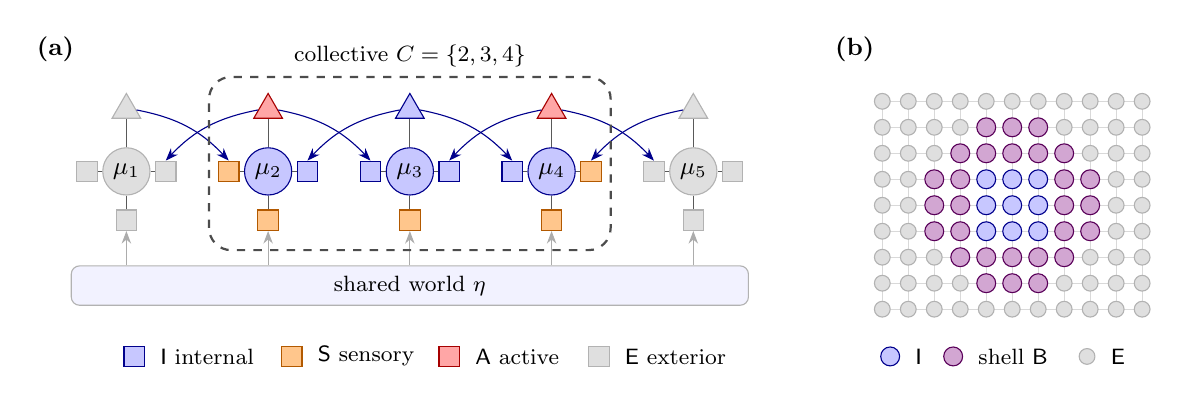
\begin{tikzpicture}[>={Stealth[length=1.6mm]}, every node/.style={font=\small},
    roleI/.style={fill=blue!22, draw=blue!55!black},
    roleS/.style={fill=orange!45, draw=orange!70!black},
    roleA/.style={fill=red!35, draw=red!65!black},
    roleE/.style={fill=gray!25, draw=gray!60},
    chan/.style={rectangle, minimum size=2.6mm, inner sep=0pt},
    outp/.style={regular polygon, regular polygon sides=3, minimum size=4.2mm, inner sep=0pt},
    intl/.style={circle, minimum size=6mm, inner sep=0pt}]
  % panel (a): chain of five agents, collective {2,3,4}
  \node[font=\small\bfseries] at (-0.9,1.55) {(a)};
  % world bar
  \node[draw=gray!60, fill=blue!5, rounded corners=3pt, minimum width=8.6cm, minimum height=0.5cm, font=\footnotesize] (world) at (3.6,-1.45) {shared world $\eta$};
  % roles: L = left input, R = right input, O = output message, M = internal, W = world sensor
  \foreach \p/\x/\L/\R/\O/\M/\W in {
      1/0.0/roleE/roleE/roleE/roleE/roleE,
      2/1.8/roleS/roleI/roleA/roleI/roleS,
      3/3.6/roleI/roleI/roleI/roleI/roleS,
      4/5.4/roleI/roleS/roleA/roleI/roleS,
      5/7.2/roleE/roleE/roleE/roleE/roleE} {
    \node[intl, \M] (M\p) at (\x,0) {$\mu_{\p}$};
    \node[chan, \L] (L\p) at (\x-0.5,0) {};
    \node[chan, \R] (R\p) at (\x+0.5,0) {};
    \node[outp, \O] (O\p) at (\x,0.78) {};
    \node[chan, \W] (W\p) at (\x,-0.62) {};
    \draw[gray!70!black] (L\p) -- (M\p);
    \draw[gray!70!black] (R\p) -- (M\p);
    \draw[gray!70!black] (W\p) -- (M\p);
    \draw[gray!70!black] (M\p) -- (O\p);
    \draw[->, gray!65] (world.north -| W\p) -- (W\p);
  }
  % messages: each output is read by both neighbors
  \foreach \p/\q in {1/2, 2/3, 3/4, 4/5} {
    \draw[->, blue!55!black, thin] (O\p.east) to[bend left=18] (L\q.north);
    \draw[->, blue!55!black, thin] (O\q.west) to[bend right=18] (R\p.north);
  }
  % collective boundary
  \draw[dashed, thick, black!70, rounded corners=8pt] (1.05,-1.0) rectangle (6.15,1.2);
  \node[anchor=south, font=\footnotesize] at (3.6,1.2) {collective $C=\{2,3,4\}$};
  % legend
  \begin{scope}[shift={(0.1,-2.35)}]
    \node[chan, roleI] (l1) at (0,0) {}; \node[right=2pt of l1, font=\footnotesize] {$\sI$ internal};
    \node[chan, roleS] (l2) at (2.0,0) {}; \node[right=2pt of l2, font=\footnotesize] {$\sS$ sensory};
    \node[chan, roleA] (l3) at (4.0,0) {}; \node[right=2pt of l3, font=\footnotesize] {$\sA$ active};
    \node[chan, roleE] (l4) at (5.9,0) {}; \node[right=2pt of l4, font=\footnotesize] {$\sE$ exterior};
  \end{scope}
  % panel (b): square lattice, interior block and a two-hop shell (Manhattan distance)
  \begin{scope}[shift={(9.6,-1.75)}]
    \node[font=\small\bfseries] at (-0.35,3.3) {(b)};
    \foreach \x in {0,...,10} \draw[gray!30] (\x*0.33,0) -- (\x*0.33,8*0.33);
    \foreach \y in {0,...,8} \draw[gray!30] (0,\y*0.33) -- (10*0.33,\y*0.33);
    \foreach \x in {0,...,10} {
      \foreach \y in {0,...,8} {
        % interior block: x in 4..6, y in 3..5; Manhattan distance to the block
        \pgfmathsetmacro{\dx}{max(0, max(4-\x, \x-6))}
        \pgfmathsetmacro{\dy}{max(0, max(3-\y, \y-5))}
        \pgfmathtruncatemacro{\dd}{\dx+\dy}
        \ifnum\dd=0
          \node[circle, inner sep=0pt, minimum size=2.4mm, roleI] at (\x*0.33,\y*0.33) {};
        \else\ifnum\dd<3
          \node[circle, inner sep=0pt, minimum size=2.4mm, fill=violet!35, draw=violet!70!black] at (\x*0.33,\y*0.33) {};
        \else
          \node[circle, inner sep=0pt, minimum size=2.0mm, roleE] at (\x*0.33,\y*0.33) {};
        \fi\fi
      }
    }
    \node[circle, inner sep=0pt, minimum size=2.4mm, roleI] (k1) at (0.1,-0.6) {}; \node[right=2pt of k1, font=\footnotesize] {$\sI$};
    \node[circle, inner sep=0pt, minimum size=2.4mm, fill=violet!35, draw=violet!70!black] (k2) at (0.9,-0.6) {}; \node[right=2pt of k2, font=\footnotesize] {shell $\sB$};
    \node[circle, inner sep=0pt, minimum size=2.0mm, roleE] (k3) at (2.6,-0.6) {}; \node[right=2pt of k3, font=\footnotesize] {$\sE$};
  \end{scope}
\end{tikzpicture}
}
  \caption{\textbf{Channel-level roles and a two-hop shell.} (a) A collective $C=\{2,3,4\}$ on a chain in which every agent reads both neighbors and senses the shared world. A member channel that reads a non-member or the world is sensory ($\sS$), a member channel read by a non-member is active ($\sA$), and every other member variable, including the internal states of boundary members and their messages to members, is internal ($\sI$). (b) One variable per site with nearest-neighbor coupling on the square lattice: an interior block, the shell of sites within two hops of it, and the exterior. With independent noise and a conditionally independent start, a shell two hops thick is an exact path blanket; a one-hop shell is not, because a shell site that reads both sides is a collider.}
  \label{fig:col-partition}
\end{figure}

Agent-level descriptions, which assign one role to each whole agent, coarsen the same variables and turn each sensing event of an interior agent into a leak; we use them only for layered partitions with one variable per agent (Supplement, \cref{rem:col-agent-level}).

\subsection{Path blankets}\label{sec:col-path}

A blanket can be asked of the stationary law at one time or of whole trajectories, and the definitions of a Markov blanket in use differ \citep{biehl2021technical}, so we declare ours.

\begin{definition}[Blankets and leaks]\label{def:col-blankets}
Let $(\sI,\sB,\sE)$ be a partition of $\mathcal V$, with $\sB=\sS\cup\sA$ when the blanket is split. The instantaneous blanket holds at round $t$ when $X_{\sI,t}\perp X_{\sE,t}\mid X_{\sB,t}$, and the path blanket holds on a window $[0,T]$ when $X_{\sI,0:T}\perp X_{\sE,0:T}\mid X_{\sB,0:T}$. For a stationary process the instantaneous leak is $\iota_{\mathrm{inst}}=I(X_{\sI,t};X_{\sE,t}\mid X_{\sB,t})$. From a declared initial law the window leak is $\iota_T=I(X_{\sI,0:T};X_{\sE,0:T}\mid X_{\sB,0:T})$, and the leak rate is $\iota_{\mathrm{path}}=\limsup_{T\to\infty}\iota_T/T$.
\end{definition}
% src: L2-D3, L2-D4, L2-R2

The path notion is that of \citet{friston2023path}, in the form conditioned on initial states of \citet{friston2023simpler}: internal and external paths are conditionally independent given blanket paths and initial states. For linear-Gaussian dynamics it has an exact characterization, with a condition that the usual statement omits.

\begin{theorem}[Path blankets]\label{thm:col-path-blanket}
Let $X$ follow \eqref{eq:col-joint} on $[0,T]$, $T\ge2$, from $X_0\sim\Ncal(\bar X_0,\Sigma_0)$ with $\Sigma_0\succ0$, independent of the noise.
\begin{enumerate}
\item[(a)] The path blanket holds on $[0,T]$ if and only if
\begin{equation}\label{eq:col-pb-general}
\begin{gathered}
((Q^{\Xi})^{-1})_{\sI\sE}=0,\quad((Q^{\Xi})^{-1}A)_{\sI\sE}=0,\quad((Q^{\Xi})^{-1}A)_{\sE\sI}=0,\\
(A^\top(Q^{\Xi})^{-1}A)_{\sI\sE}=0,\quad(\Sigma_0^{-1})_{\sI\sE}=0.
\end{gathered}
\end{equation}
If the noise is independent across the partition, these conditions are equivalent to
\begin{equation}\label{eq:col-pb}
A_{\sI\sE}=0,\qquad A_{\sE\sI}=0,\qquad A_{\sB\sI}^\top(Q^{\Xi}_{\sB\sB})^{-1}A_{\sB\sE}=0,\qquad X_{\sI,0}\perp X_{\sE,0}\mid X_{\sB,0}.
\end{equation}
Sufficiency does not need a Gaussian start: under the first four conditions of \eqref{eq:col-pb-general} the path blanket holds on $[0,T]$ from every initial law, independent of the noise, under which $X_{\sI,0}\perp X_{\sE,0}\mid X_{\sB,0}$.
\item[(b)] For the canonical partition of a set of agents with per-channel noise, the first two conditions of \eqref{eq:col-pb} hold by construction and the third reads $\sum_{k\in\sS}A_{k\sI}^\top(Q^{\Xi}_{kk})^{-1}A_{k\sE}=0$. It holds when no sensory channel reads both an interior and an exterior variable in the same round; if one does, it fails outside a set of coefficients of positive codimension. In particular, if every member hears every source through a separate channel, every set of agents is an exact path blanket under its canonical partition from every start with $X_{\sI,0}\perp X_{\sE,0}\mid X_{\sB,0}$.
\item[(c)] If the noise is independent across the partition and the first three conditions of \eqref{eq:col-pb} hold, then from every initial law with a density the window leak is the initial-slice term, $\iota_T=I(X_{\sI,0};X_{\sE,0}\mid X_{\sB,0:T})$. If in addition $\rho(A)<1$ and $X_0$ is Gaussian with $\Sigma_0\succ0$, the stationary law for example, then
\begin{equation}\label{eq:col-initial-slice}
\sup_T\iota_T\le I(X_{\sI,0};X_{\sB,0},X_{\sE,0})+\tfrac12\Vert\Sigma_0\Vert(1+\Vert A\Vert)^2\Vert(Q^{\Xi})^{-1}\Vert\sum_{t\ge1}\Vert A^t\Vert_F^2<\infty,
\end{equation}
so the leak rate is zero.
\end{enumerate}
\end{theorem}
% src: L2-T1, L2-L1, L2-P1, L6-P1(a),(c), C_critic V1
Proof in \cref{app:col}; checked on small systems in \cref{chk:col-path}. The condition that the usual statement omits is the third of \eqref{eq:col-pb}. A blanket variable that reads both sides in one round is a common child of interior and exterior, and conditioning on it couples them \citep{pearl1988probabilistic}. With channel-level roles and per-channel noise only a sensory channel that superposes sources from both sides can be such a collider: one acoustic channel carrying an insider's and an outsider's voice, a price formed by orders from inside and outside a firm, an archive written by both. By (c) a stationary path blanket leaks only through its first time slice, so stationary statements are made through the leak rate.

In the simplest collider, three scalar variables of which the blanket variable reads the other two, the path blanket fails on every window of two or more rounds, and the leak rate is $0.1438$ nats per round at unit coefficients and unit noise variances (Supplement, \cref{ex:col-collider}).

In agent-level descriptions with one variable per agent, one-hop local coupling and per-agent noise, every partition whose interior and exterior are at least three hops apart is an exact path blanket from every start that satisfies the blanket at the initial time, and a shell one agent thick is exact only under a cancellation condition that fails outside a set of positive codimension when a shell agent reads both sides (Supplement, \cref{prop:col-two-hop}). This is \cref{fig:col-partition}(b): a second layer separates the readers of the interior from those of the exterior.

\begin{proposition}[Records in the partition]\label{prop:col-records-partition}
Let the joint process \eqref{eq:col-joint} have per-channel noise and records as in \cref{def:col-partition}.
\begin{enumerate}
\item[(a)] The canonical partition, with records assigned as there, is an exact path blanket on every window, from every start with $X_{\sI,0}\perp X_{\sE,0}\mid X_{\sB,0}$ and for every persistence of the records, if and only if the collider condition of \cref{thm:col-path-blanket}(b) holds. The lags that records introduce need no further condition while records are kept as state variables.
\item[(b)] Other placements fail in general. A record read by an outsider and placed in $\sI$ violates $A_{\sE\sI}=0$. A record written from both sides and placed in $\sB$ makes the member channels that write only it internal, so that the record reads an interior and an exterior variable in one round, a collider. An exterior record written only by non-members may instead be placed in $\sS$, which changes what is conditioned on and not exactness.
\end{enumerate}
\end{proposition}
% src: B5-D2, B5-P6
Proof in \cref{app:col}; checked at agent level in \cref{chk:col-records}. An agent-level description that marginalizes a record written inside and read outside turns it into a lagged coupling, which leaks (\cref{sec:agy}).

\subsection{Stationary blankets and the Markov length}\label{sec:col-markov}

A stationary blanket asks that the stationary law at one time factor across the shell. For the joint law that includes the world this can fail even when the path blanket holds, and the reason is memory.

When the path blanket holds on every window, the instantaneous leak is bounded by the memory of either side, in the Gaussian case adding the boundary's filtered estimate of the exterior to the blanket restores an exact instantaneous blanket, and for reversible dynamics with noise independent across the partition the stationary instantaneous blanket holds exactly when the collider condition of \cref{thm:col-path-blanket} does, under the hypotheses stated there (Supplement, \cref{prop:col-memory}). Agents that sense an exogenous world never form a reversible process, so we condition on the world, which removes its memory; the remaining stationary law has blankets whose thickness is measured by a length of its own.

\begin{definition}[Markov length]\label{def:col-markov-length}
For a stationary law of variables $e_i$ on the vertices of a graph with hop distance $d$, a vertex $i$ and a width $h\ge1$, let $\sB_h(i)=\{j:1\le d(i,j)\le h\}$, $\sE_h(i)=\{j:d(i,j)>h\}$ and $\iota(i,h)=I(e_i;e_{\sE_h(i)}\mid e_{\sB_h(i)})$. The Markov length $\xi_M$ is the infimum of the $\xi'>0$ for which $\sup_i\iota(i,h)\le B'e^{-h/\xi'}$ for some constant $B'$ and all $h$. On $\Z$ the one-sided Markov length is defined in the same way from $I(e_{\le0};e_{\ge h+1}\mid e_{1:h})$.
\end{definition}
% src: L6-D2
This adapts the Markov length that \citet{sang2025stability} define for quantum states. A law whose conditional mutual information vanishes beyond a finite width has $\xi_M=0$.

Consider a Gaussian law on a graph of polynomial growth, with at most $B_{\mathcal G}r^{D-1}$ vertices at hop distance $r$ from any vertex, whose covariance decays exponentially and is bounded with bounded inverse. Under the hypotheses stated there, the precision decays exponentially at an explicit smaller rate $m_\Pi$, the instantaneous leak across a shell of width $h$, one that keeps a finite interior at least $h$ hops from the exterior with at most $n_\partial$ interior vertices at each distance from the exterior, is $O(n_\partial h^{D-1}e^{-2m_\Pi h})$, and $\xi_M\le1/(2m_\Pi)$ (Supplement, \cref{thm:col-thick-shell,thm:col-markov-bound}). The bound depends on the decay of the covariance and on its conditioning, and no bound by the correlation length alone is possible.

\begin{proposition}[Markov length and correlation length]\label{prop:col-markov-vs-correlation}
\begin{enumerate}
\item[(a)] (Hub family.) On a path graph place listeners at the even positions $2k$ and memoryless sources at the odd positions $2k+1$, $k\in\Z$. Sources attend no one, $e^{\mathrm{src}}_k(t+1)=\zeta^{\mathrm{src}}_k(t)$ with variance $q_{\mathrm{src}}$. Listener $k$ attends sources $k-1$ and $k$ with message weight $a\in(0,\frac12)$ and self weight $c=0$, $e^{\mathrm{lis}}_k(t+1)=a[e^{\mathrm{src}}_{k-1}(t)+e^{\mathrm{src}}_k(t)]+\zeta^{\mathrm{lis}}_k(t)$ with variance $q_{\mathrm{lis}}$. The weights are nonnegative, the noise is local and the row sums are at most $\lambda=2a<1$. The stationary covariance vanishes between agents more than two hops apart, so $\xi=0$, while with $\psi=q_{\mathrm{lis}}/(a^2q_{\mathrm{src}})$ the Markov length is exactly $1/\arccosh(1+\psi/2)$ hops, which is $\psi^{-1/2}(1+O(\psi))$ as $\psi\to0$; when $q_{\mathrm{lis}}\le(1-4a^2)q_{\mathrm{src}}$ the condition number of $\Sigma$ is $\operatorname{cond}(\Sigma)=1/(a^2\psi)$. Hence there is no constant $B$ with $\xi_M\le B\xi$ in the class of local noise and row-sum contraction, and in this family $\xi_M$ grows like $a\operatorname{cond}(\Sigma)^{1/2}$.
\item[(b)] (Moving average.) The stationary Gaussian field $Y_i=Z_i+\alpha Z_{i-1}$ on $\Z$, with independent standard normal $Z_i$ and $0<\alpha\le1$, has covariance range one. The partial correlation of $Y_0$ and $Y_{h+1}$ given the $h$ sites between them is $\alpha^{h+1}(1-\alpha^2)/(1-\alpha^{2(h+2)})$ for $\alpha<1$ and $1/(h+2)$ for $\alpha=1$, so the one-sided Markov length is at least $1/(2\ln(1/\alpha))$ and is infinite at $\alpha=1$.
\item[(c)] (Massless limit.) For nearest-neighbor passing on $\Z^D$, $W_{ii}=c$ and $W_{ij}=a$ between lattice neighbors with $Q^{\zeta}=qI$, the Ornstein--Zernike length $1/\arccosh(1+\varepsilon/(2a))$ diverges as the leak $\varepsilon=1-c-2Da$ tends to zero (\cref{thm:sca-oz}), while every region with $d(\sI,\sE)\ge3$ is an exact stationary blanket of the world-conditional law and $\xi_M=0$.
\end{enumerate}
\end{proposition}
% src: B3-P5, L6-P4(a),(c), C_critic V2, C2-7, B1-T4(c)
Proof in \cref{app:col}; all three parts are checked in \cref{chk:col-markov}. \Cref{fig:col-markov} shows both directions of the independence: in the hub family $\xi_M$ diverges as $\psi\to0$ while $\xi=0$, and under nearest-neighbor passing on a ring $\xi$ diverges as $\varepsilon\to0$ while $\xi_M=0$.

\begin{figure}[t]
  \centering
  % Figure: the Markov length and the correlation length are independent (prop:col-markov-vs-correlation).
% (a) Hub family, a = 0.45, q_src = 1: xi_M = 1/arccosh(1 + psi/2) (closed form of the proposition), its
% asymptote psi^{-1/2}, and Markov lengths fitted from the conditional mutual information iota(i, h) of
% def:col-markov-length, recomputed from Lyapunov solves of the full network as in chk:col-markov:
% circles, log-linear fit over widths h = 1..30 on a path of 401 agents (0.567, 1.036, 3.154, 9.36 hops);
% crosses, fit over the last ten even widths up to 40 on 241 positions (0.567, 1.039, 3.175, 9.993 hops).
% Covariances vanish exactly beyond two hops in every solve, so xi = 0.
% (b) Nearest-neighbor passing on a ring, W_ii = c, W_ij = a, leak eps = 1 - c - 2a:
% xi = 1/arccosh(1 + eps/(2a)) (thm:sca-oz) for c = 0.3 and c = 0; dots at eps = 1e-3, xi = 18.70 and 22.35 hops.
% On a ring of 120 agents at eps = 1e-3 the conditional mutual information across a shell of width h is 5.35e-2
% (c = 0.3) at h = 1 and below 4e-14 in magnitude at h = 2, 3, 6, so xi_M = 0.
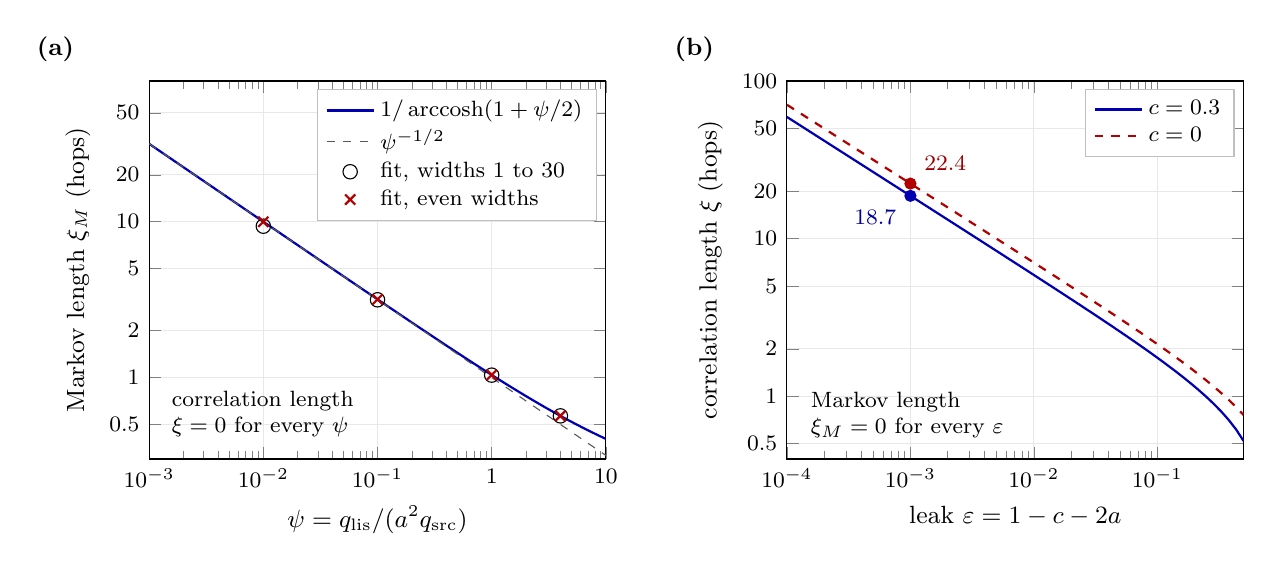
\begin{tikzpicture}
  \pgfplotsset{markovframe/.style={width=5.8cm, height=4.8cm, scale only axis,
      every axis label/.style={font=\small}, tick label style={font=\footnotesize},
      grid=major, grid style={gray!18}, log ticks with fixed point,
      legend style={font=\footnotesize, draw=gray!50, fill=white, cells={anchor=west}, row sep=-1pt}}}
  % ---------------- panel (a): hub family
  \begin{loglogaxis}[markovframe, name=hub, xmin=1e-3, xmax=10, ymin=0.3, ymax=80,
      xtick={0.001,0.01,0.1,1,10}, xticklabels={$10^{-3}$,$10^{-2}$,$10^{-1}$,$1$,$10$},
      ytick={0.5,1,2,5,10,20,50},
      xlabel={$\psi=q_{\mathrm{lis}}/(a^2q_{\mathrm{src}})$}, ylabel={Markov length $\xi_M$ (hops)},
      legend style={at={(0.98,0.98)}, anchor=north east}]
    \addplot[blue!70!black, thick] coordinates {(0.001,31.6241) (0.00116591,29.2879) (0.00135936,27.1243) (0.00158489,25.1205) (0.00184785,23.2648) (0.00215443,21.5463) (0.00251189,19.9547) (0.00292864,18.4808) (0.00341455,17.1157) (0.00398107,15.8516) (0.00464159,14.6808) (0.0054117,13.5966) (0.00630957,12.5926) (0.00735642,11.6627) (0.00857696,10.8016) (0.01,10.0042) (0.0116591,9.26568) (0.0135936,8.58181) (0.0158489,7.94852) (0.0184785,7.36208) (0.0215443,6.81903) (0.0251189,6.31617) (0.0292864,5.85053) (0.0341455,5.41938) (0.0398107,5.02016) (0.0464159,4.65054) (0.054117,4.30832) (0.0630957,3.99149) (0.0735642,3.69819) (0.0857696,3.42668) (0.1,3.17536) (0.116591,2.94276) (0.135936,2.72749) (0.158489,2.52829) (0.184785,2.34399) (0.215443,2.17349) (0.251189,2.01579) (0.292864,1.86995) (0.341455,1.73511) (0.398107,1.61048) (0.464159,1.49531) (0.54117,1.38891) (0.630957,1.29065) (0.735642,1.19995) (0.857696,1.11625) (1,1.03904) (1.16591,0.967865) (1.35936,0.902273) (1.58489,0.841858) (1.84785,0.786239) (2.15443,0.735059) (2.51189,0.687986) (2.92864,0.644706) (3.41455,0.604928) (3.98107,0.568377) (4.64159,0.534797) (5.4117,0.503947) (6.30957,0.475601) (7.35642,0.449552) (8.57696,0.425601) (10,0.403569)};
    \addlegendentry{$1/\arccosh(1+\psi/2)$}
    \addplot[gray!70!black, dashed] coordinates {(0.001,31.6228) (0.00116591,29.2864) (0.00135936,27.1227) (0.00158489,25.1189) (0.00184785,23.2631) (0.00215443,21.5443) (0.00251189,19.9526) (0.00292864,18.4785) (0.00341455,17.1133) (0.00398107,15.8489) (0.00464159,14.678) (0.0054117,13.5936) (0.00630957,12.5893) (0.00735642,11.6591) (0.00857696,10.7978) (0.01,10) (0.0116591,9.26119) (0.0135936,8.57696) (0.0158489,7.94328) (0.0184785,7.35642) (0.0215443,6.81292) (0.0251189,6.30957) (0.0292864,5.84341) (0.0341455,5.4117) (0.0398107,5.01187) (0.0464159,4.64159) (0.054117,4.29866) (0.0630957,3.98107) (0.0735642,3.68695) (0.0857696,3.41455) (0.1,3.16228) (0.116591,2.92864) (0.135936,2.71227) (0.158489,2.51189) (0.184785,2.32631) (0.215443,2.15443) (0.251189,1.99526) (0.292864,1.84785) (0.341455,1.71133) (0.398107,1.58489) (0.464159,1.4678) (0.54117,1.35936) (0.630957,1.25893) (0.735642,1.16591) (0.857696,1.07978) (1,1) (1.16591,0.926119) (1.35936,0.857696) (1.58489,0.794328) (1.84785,0.735642) (2.15443,0.681292) (2.51189,0.630957) (2.92864,0.584341) (3.41455,0.54117) (3.98107,0.501187) (4.64159,0.464159) (5.4117,0.429866) (6.30957,0.398107) (7.35642,0.368695) (8.57696,0.341455) (10,0.316228)};
    \addlegendentry{$\psi^{-1/2}$}
    \addplot[only marks, mark=o, mark size=2.6pt, black] coordinates {(4,0.5673) (1,1.036) (0.1,3.154) (0.01,9.359)};
    \addlegendentry{fit, widths $1$ to $30$}
    \addplot[only marks, mark=x, mark size=2.6pt, red!70!black, thick] coordinates {(4,0.5673) (1,1.039) (0.1,3.175) (0.01,9.993)};
    \addlegendentry{fit, even widths}
    \node[font=\footnotesize, anchor=south west, align=left] at (axis cs:0.0013,0.36) {correlation length\\$\xi=0$ for every $\psi$};
  \end{loglogaxis}
  \node[font=\small\bfseries, anchor=south west] at ([xshift=-1.55cm, yshift=0.12cm]hub.north west) {(a)};
  % ---------------- panel (b): nearest-neighbor passing on a ring
  \begin{loglogaxis}[markovframe, name=ring, at={($(hub.north east)+(2.3cm,0)$)}, anchor=north west,
      xmin=1e-4, xmax=0.5, ymin=0.4, ymax=100,
      xtick={0.0001,0.001,0.01,0.1}, xticklabels={$10^{-4}$,$10^{-3}$,$10^{-2}$,$10^{-1}$},
      ytick={0.5,1,2,5,10,20,50,100},
      xlabel={leak $\varepsilon=1-c-2a$}, ylabel={correlation length $\xi$ (hops)},
      legend style={at={(0.98,0.98)}, anchor=north east}]
    \addplot[blue!70!black, thick] coordinates {(0.0001,59.1573) (0.000115252,55.1035) (0.000132831,51.3275) (0.000153091,47.8102) (0.00017644,44.5338) (0.000203352,41.4818) (0.000234367,38.6389) (0.000270114,35.9908) (0.000311312,33.524) (0.000358794,31.2262) (0.000413519,29.0857) (0.00047659,27.0918) (0.00054928,25.2345) (0.000633058,23.5044) (0.000729614,21.8927) (0.000840896,20.3913) (0.000969152,18.9927) (0.00111697,17.6899) (0.00128733,16.4761) (0.00148368,15.3455) (0.00170998,14.2921) (0.00197079,13.3108) (0.00227138,12.3966) (0.00261781,11.5448) (0.00301709,10.7512) (0.00347726,10.0119) (0.00400762,9.32292) (0.00461888,8.68097) (0.00532336,8.08277) (0.0061353,7.52531) (0.00707107,7.00576) (0.00814957,6.52153) (0.00939256,6.07015) (0.0108251,5.64937) (0.0124762,5.25705) (0.0143791,4.89122) (0.0165723,4.55003) (0.0190999,4.23176) (0.0220131,3.93481) (0.0253706,3.65767) (0.0292402,3.39894) (0.0337,3.15732) (0.03884,2.93158) (0.044764,2.72058) (0.0515915,2.52324) (0.0594604,2.33856) (0.0685294,2.16558) (0.0789817,2.00342) (0.0910282,1.85124) (0.104912,1.70823) (0.120914,1.57363) (0.139356,1.4467) (0.160611,1.32673) (0.185107,1.213) (0.21334,1.10481) (0.24588,1.0014) (0.283382,0.901961) (0.326604,0.805555) (0.376419,0.710994) (0.433831,0.616593) (0.5,0.519522)};
    \addlegendentry{$c=0.3$}
    \addplot[red!70!black, thick, dashed] coordinates {(0.0001,70.7077) (0.000115252,65.8627) (0.000132831,61.3496) (0.000153091,57.1456) (0.00017644,53.2297) (0.000203352,49.582) (0.000234367,46.1843) (0.000270114,43.0193) (0.000311312,40.071) (0.000358794,37.3248) (0.000413519,34.7666) (0.00047659,32.3837) (0.00054928,30.164) (0.000633058,28.0963) (0.000729614,26.1702) (0.000840896,24.3759) (0.000969152,22.7046) (0.00111697,21.1476) (0.00128733,19.6973) (0.00148368,18.3462) (0.00170998,17.0876) (0.00197079,15.9151) (0.00227138,14.8228) (0.00261781,13.8052) (0.00301709,12.8571) (0.00347726,11.9739) (0.00400762,11.151) (0.00461888,10.3843) (0.00532336,9.67) (0.0061353,9.00438) (0.00707107,8.38415) (0.00814957,7.80617) (0.00939256,7.26752) (0.0108251,6.7655) (0.0124762,6.29758) (0.0143791,5.86139) (0.0165723,5.45473) (0.0190999,5.07556) (0.0220131,4.72196) (0.0253706,4.39215) (0.0292402,4.08446) (0.0337,3.79735) (0.03884,3.52935) (0.044764,3.27912) (0.0515915,3.04539) (0.0594604,2.82697) (0.0685294,2.62276) (0.0789817,2.43171) (0.0910282,2.25285) (0.104912,2.08525) (0.120914,1.92806) (0.139356,1.78044) (0.160611,1.64162) (0.185107,1.51085) (0.21334,1.3874) (0.24588,1.27056) (0.283382,1.15962) (0.326604,1.05386) (0.376419,0.952493) (0.433831,0.854662) (0.5,0.759326)};
    \addlegendentry{$c=0$}
    \addplot[only marks, mark=*, mark size=2.0pt, blue!70!black, forget plot] coordinates {(0.001,18.697)};
    \addplot[only marks, mark=*, mark size=2.0pt, red!70!black, forget plot] coordinates {(0.001,22.351)};
    \node[font=\footnotesize, blue!60!black, anchor=north east] at (axis cs:0.00092,17.4) {$18.7$};
    \node[font=\footnotesize, red!60!black, anchor=south west] at (axis cs:0.00108,23.6) {$22.4$};
    \node[font=\footnotesize, anchor=south west, align=left] at (axis cs:0.00013,0.47) {Markov length\\$\xi_M=0$ for every $\varepsilon$};
  \end{loglogaxis}
  \node[font=\small\bfseries, anchor=south west] at ([xshift=-1.55cm, yshift=0.12cm]ring.north west) {(b)};
\end{tikzpicture}

  \caption{\textbf{The Markov length and the correlation length are independent.} (a) The hub family of \cref{prop:col-markov-vs-correlation}(a) with $a=0.45$. The Markov length $\xi_M=1/\arccosh(1+\psi/2)$ grows like $\psi^{-1/2}$ (dashed) as $\psi$ falls, while covariances vanish beyond two hops and the correlation length is $\xi=0$ at every $\psi$. Marks are Markov lengths fitted to the conditional mutual information $\iota(i,h)$ of \cref{def:col-markov-length}, computed from Lyapunov solves of the whole network (\cref{chk:col-markov}): circles from a fit over widths $1$ to $30$ on a path of $401$ agents, crosses from a fit over the last ten even widths up to $40$ on $241$ positions. The circle at $\psi=0.01$, at $9.36$ hops against $10.00$, comes from a window of widths that is not yet asymptotic. (b) Nearest-neighbor passing on a ring, $W_{ii}=c$ and $W_{ij}=a$ between neighbors with $Q^\zeta=qI$, and leak $\varepsilon=1-c-2a$. The correlation length $\xi=1/\arccosh(1+\varepsilon/(2a))$, which in one dimension is the decay length of the covariance itself and equals the Ornstein--Zernike length (\cref{thm:sca-oz}(e)), diverges as $\varepsilon\to0$ and reaches $18.7$ hops at $c=0.3$ and $22.4$ hops at $c=0$ when $\varepsilon=10^{-3}$ (dots), while shells two hops thick are exact stationary blankets of the world-conditional law at every leak, so that $\xi_M=0$ (\cref{prop:col-markov-vs-correlation}(c)).}
  \label{fig:col-markov}
\end{figure}

The hub family also shows that a bound on $\xi_M$ must depend on conditioning. It is conjectured that for time-invariant networks on $\Z^D$ with local noise and row-sum contraction the Markov length is at most $1+\xi$ times a function of the noise anisotropy, the error dimension and $D$, and a numerical observation near the massless limit, where $\xi$ diverges, is consistent with this (Supplement, \cref{conj:col-markov-length,obs:col-massless}). An earlier formulation of H1 in terms of the correlation length, false in both directions by \cref{prop:col-markov-vs-correlation}, is corrected in \cref{rem:col-shell-error} of the Supplement.

Collected, these results show that the existence of a blanket cannot select a collective: under per-channel noise with separate channels every set of agents has an exact path blanket under its canonical partition, every set with a two-hop shell has one under one-hop coupling with per-agent noise, thick shells give approximate instantaneous blankets under the hypotheses of \cref{thm:col-thick-shell}, and in a translation-invariant medium no rule based on blankets or leaks separates a region from its translates (Supplement, \cref{sec:col-selects}, \cref{prop:col-selects-nothing}). Selection needs another criterion; \cref{thm:col-boundary} states the boundary property in final form.

\subsection{The world-conditional law and when its precision is diffusive}\label{sec:col-world}

Every agent senses the same world, so the unconditional correlations of members' errors contain a common mode generated by the world's innovations (\cref{lem:fw-common-mode}). That component is shared input, not interaction, and a collective must not be read off it. We therefore condition on the world path.

\begin{definition}[World-conditional law]\label{def:col-world-conditional}
Let the agents' errors $e(t)=(e_i(t))_{i\in V}$ and the world path $(\eta_t)_{t\in\Z}$ be jointly stationary. The world-conditional law of the errors is their regular conditional law given the whole world path, with every channel noise shared by several receivers, the sender-side noise of a broadcast, added to the conditioning set, so that the remaining local noise is specific to each receiver. Records written by agents belong to the conditioned process and are not conditioned on. When this law is Gaussian with a covariance $\Sigma^c$ that does not depend on the realized path, $\Sigma^c$ is the world-conditional covariance and, when $\Sigma^c\succ0$, $\Pi^c=(\Sigma^c)^{-1}$ is the world-conditional precision.
\end{definition}
% src: B1-D1, B5-D1, decision 2, decision 13

\begin{proposition}[The world-conditional law of the level-0 network]\label{prop:col-world-conditional}
Let the level-0 network of \cref{def:fw-level0}, with code models that may be wrong, satisfy the hypotheses of \cref{lem:fw-common-mode} with a stationary world, $\rho(F)<1$, so that \cref{def:col-world-conditional} applies, and let its local noise $\zeta(t)$ be Gaussian with covariance $Q^\zeta$. Then the world-conditional law of the stationary error path is the conditional law of \cref{lem:fw-common-mode}(c): it is Gaussian, with mean the common part $e^{\mathrm{com}}$ of \eqref{eq:fw-common-mode}, mistranslation term $B^{\mathrm{mis}}$ included, and around it the law of the connected part $e^{\mathrm{loc}}$. Its covariance at one time is the covariance $\Sigma^{\mathrm{loc}}$ of \cref{lem:fw-common-mode}(b),
\begin{equation}\label{eq:col-sigma-c}
\Sigma^c=\Sigma^{\mathrm{loc}}=\sum_{n\ge0}W^nQ^\zeta(W^\top)^n,
\end{equation}
which does not depend on the path. If channel noises shared by several receivers enter the error recursion, the same holds with their response added to the mean, because \cref{def:col-world-conditional} conditions on them.
\end{proposition}
% src: B1-P1, L3-L1, C2-1; stated through lem:fw-common-mode, which owns the level-0 network and its common mode
Proof in \cref{app:col}; checked in \cref{chk:col-world}. Every length statement of \cref{sec:sca} about the error recursion with local noise is therefore a statement about the world-conditional law.

The definition applies verbatim to receivers that fuse exactly, although $\Sigma^c$ then no longer solves a Lyapunov equation in the members' states, and records enter the world-conditional law as nodes (Supplement, \cref{rem:col-world-conditional}).

A symmetric positive definite matrix $\Pi$ on a set of agents is diffusive when
\begin{equation}\label{eq:col-diffusive}
\Pi=\diag(\varepsilon^\Pi)+L^\Pi,\qquad(L^\Pi f)_i=\sum_ja^\Pi_{ij}(f_i-f_j),\qquad a^\Pi_{ij}=a^\Pi_{ji}\ge0,\qquad\varepsilon^\Pi_i\ge0,
\end{equation}
that is, when $\Pi$ has nonpositive off-diagonal entries and nonnegative row sums; then $a^\Pi_{ij}=-\Pi_{ij}$ and $\varepsilon^\Pi_i=(\Pi\one)_i$. The couplings may have any range. A diffusive precision describes a Gaussian field in which each agent's error is pulled toward those of the agents it is coupled to, with weights $a^\Pi_{ij}$, and toward zero with weight $\varepsilon^\Pi_i$, the leak that collects grounding and forgetting.

\begin{theorem}[Diffusive world-conditional precisions]\label{thm:col-diffusive-precision}
Let $\rho(W)<1$ and let $Q^{\zeta}\succ0$ be block diagonal over agents. For scalar errors write $Q^{\zeta}=\diag(q_i)$, $\lambda_i=(W\one)_i$ and $\lambda^{\mathrm{col}}_i=(\one^\top W)_i$.
\begin{enumerate}
\item[(a)] (Reversible case.) If $WQ^{\zeta}=Q^{\zeta}W^\top$, then $\Sigma^c=(I-W^2)^{-1}Q^{\zeta}$ and $\Pi^c=(Q^{\zeta})^{-1}-W^\top(Q^{\zeta})^{-1}W$. For scalar errors
\begin{equation}\label{eq:col-pi-rev}
a^\Pi_{ij}=\sum_k\frac{W_{ki}W_{kj}}{q_k}\quad(i\neq j),\qquad\varepsilon^\Pi_i=\frac{1-\sum_kW_{ik}\lambda_k}{q_i},
\end{equation}
and if in addition $W\ge0$ entrywise with every row sum at most $\lambda<1$, then $\Pi^c$ is diffusive with $\varepsilon^\Pi_i\ge(1-\lambda^2)/q_i$.
\item[(b)] (Normal case with isotropic noise.) If $WW^\top=W^\top W$ and $Q^{\zeta}=qI$, then $\Sigma^c=q(I-WW^\top)^{-1}$ and $\Pi^c=(I-WW^\top)/q$. For scalar errors
\begin{equation}\label{eq:col-pi-normal}
a^\Pi_{ij}=\frac1q\sum_kW_{ik}W_{jk}\quad(i\neq j),\qquad\varepsilon^\Pi_i=\frac{1-\sum_kW_{ik}\lambda^{\mathrm{col}}_k}{q},
\end{equation}
and if in addition $W\ge0$, then $\Pi^c$ is diffusive exactly when $\sum_kW_{ik}\lambda^{\mathrm{col}}_k\le1$ for every $i$, in particular when the largest row sum times the largest column sum is at most one.
\item[(c)] (Range two.) In both cases, for vector as for scalar errors and whatever the signs of the weights, a block $\Pi^c_{ij}$ with $i\neq j$ vanishes unless $i$ and $j$ have a common neighbor in the attention graph, an agent counting as attending itself. In the reversible case the common neighbor is a listener: $\Pi^c_{ij}$ vanishes unless some agent $k$ attends both $i$ and $j$, $W_{ki}\neq0$ and $W_{kj}\neq0$. In the normal case it is a source: $\Pi^c_{ij}$ vanishes unless $i$ and $j$ both attend some agent $k$, $W_{ik}\neq0$ and $W_{jk}\neq0$. Every partition with $d(\sI,\sE)\ge3$ in the attention graph is then an exact stationary blanket of the world-conditional law.
\item[(d)] (Level zero.) For scalar level-0 receivers with exact code models, $W_{ij}=Fk_{ij}$, $W_{ii}=F(1-k^s_i-\sum_jk_{ij})$ and $\lambda_i=F(1-k^s_i)$; reversibility reads $k_{ij}q_j=q_ik_{ji}$, and with a common sensing gain $k^s$ the leaks are $(1-\lambda^2)/q_i$ in either case, with $\lambda=F(1-k^s)$.
\item[(e)] (Nearest-neighbor passing.) For $W_{ii}=c$ and $W_{ij}=a$ between lattice neighbors on $\Z^D$, with $Q^{\zeta}=qI$, the couplings of $\Pi^c$ are $2ca/q$ at axis distance one, $a^2/q$ at axis distance two and $2a^2/q$ at each diagonal neighbor, displaced by one site in each of two coordinates, and the leak is $(1-\lambda^2)/q$ with $\lambda=c+2Da$.
\end{enumerate}
\end{theorem}
% src: B1-T1, L2-P4, L2-R1, L6-P2, C2-1; (c) stated for vector errors, which the proof covers
Proof in \cref{app:col}; checked in \cref{chk:col-diffusive}. The couplings of $\Pi^c$ join agents that share a listener or a source, an agent being its own listener and source, so they have range two in the attention graph. Grounding enters through the leak: with a common sensing gain the row sums $\lambda=F(1-k^s)$ fall as agents sense more, and $\varepsilon^\Pi$ rises. Diffusivity is not automatic.

A common listener gives two sources that attend no one a positive off-diagonal entry of $\Pi^c$, signed weights can do the same, and such entries occurred in $674$ of $2000$ random directed nonnegative draws on four agents (Supplement, \cref{ex:col-non-diffusive}). Non-reciprocal attention, which the agents' own choices produce, can therefore leave the diffusive class.

Two problems are open: to define contrast, and to prove a size bound, for world-conditional precisions with positive off-diagonal entries, for which contrast is until then not defined and the available substitutes are named in the statement, and to decide whether the world-conditional precision of receivers that fuse exactly is diffusive (Supplement, \cref{open:col-non-diffusive,open:col-exact-fusion}).

\subsection{Contrast, the homogeneous baseline and the definition of a collective}\label{sec:col-contrast}

Blankets do not select collectives; contrast does. We define it on the world-conditional precision, fix the baseline that it must exceed, and then define a collective.

\begin{definition}[Contrast]\label{def:col-contrast}
Let $\Pi^c=\diag(\varepsilon^\Pi)+L^\Pi$ be a diffusive world-conditional precision of the whole population, records included. For a finite region $C\subseteq V$ with $n=|C|\ge2$, let $\phi_C=\one_C/\sqrt n$, let $L_C$ be the Laplacian of the couplings inside $C$, let $a^\partial_i=\sum_{k\notin C}a^\Pi_{ik}$ be the cut coupling of member $i$, and put $\cut(C)=\sum_{i\in C}a^\partial_i$. The rates of $C$ are
\begin{equation}\label{eq:col-rates}
\xout(C)=\phi_C^\top\Pi^c\phi_C=\bar\varepsilon_C+\frac{\cut(C)}{n},\qquad\xin(C)=\min_{\substack{f\perp\one_C\\\operatorname{supp}f\subseteq C}}\frac{f^\top(\diag(\varepsilon^\Pi)+L_C)f}{f^\top f},
\end{equation}
with $\bar\varepsilon_C$ and $\varepsilon^{\max}_C$ the mean and the largest leak on $C$. The contrast of $C$ is $r(C)=\xin(C)/\xout(C)$, and its grounding-free ratio is $r_\star(C)=\lambda_2(L_C)/(\cut(C)/n)$. For vector errors whose world-conditional covariance has the form $\Sigma^{\mathrm{sc}}\otimes I_K$, with agent indices first, contrast is computed from the scalar precision $(\Sigma^{\mathrm{sc}})^{-1}$. When attention is drawn at random in every round and the world-conditional law is a mixture of Gaussian laws, $\Sigma^c$ denotes its second moment $\E[\Cov(e(t)\mid\eta)]$.
\end{definition}
% src: B1-D2, L2-D7, decision 2, decision 13, C2-5 (second-moment and per-coordinate declarations)

For the reversible diffusion with drift $-\Pi^c$, whose stationary covariance is $\Sigma^c$, $\xout$ is the rate at which the members' average relaxes and $\xin$ the slowest relaxation rate of internal disagreement, so a region with $r\gg1$ has a freely fluctuating collective coordinate and pinned internal disagreements. The statistical reading of the two rates and their relation to the drift-based contrast of \cref{thm:agy-closure-average}, which can differ from $r$ even for reversible drift, are in the Supplement (\cref{sup:col-scope-and-reading-of-contrast}).

For a diffusive positive definite precision on a finite set, the precision of the members' marginal law is again diffusive, and the contrast $r'(C)$ computed from it satisfies $r'(C)\ge r(C)$ (Supplement, \cref{lem:col-kron}).

The inequality $r'\ge r$ can be strict by a large factor. We compute contrast from the whole population's precision, the conservative choice; the marginal contrast is an upper bound for an analyst who observes only the members (Supplement, \cref{rem:col-which-contrast}).

\begin{definition}[Homogeneous baseline]\label{def:col-baseline}
The comparison medium of a population is declared with the model. It keeps the population's declared geometry, replaces couplings and leaks by their means, except for couplings generated by a declared mechanism under clause (c), and is closed when the population is closed. Let $\bar\varepsilon$ be the mean leak of the population.
\begin{enumerate}
\item[(a)] (Lattice.) If the agents occupy the sites of $\Z^D$ or of a finite box or torus of $\Z^D$, the displacement class of $x$ is the set of pairs of sites whose difference is $\pm x$, modulo the torus on a torus. The comparison medium has the same sites, gives every pair of the class of $x$ the mean $\bar a(x)$ of $a^\Pi_{ij}$ over the pairs of that class, and has uniform leak $\bar\varepsilon$. On $\Z^D$ the means are limits of averages over growing boxes, and the clause applies when they exist.
\item[(b)] (Interaction graph.) If the model declares no lattice but an interaction graph on $V$ whose edge set $E_{\mathrm d}$ contains every pair of positive coupling, the comparison medium is that graph with the mean coupling $\bar a_{\mathrm d}=|E_{\mathrm d}|^{-1}\sum_{\{i,j\}\in E_{\mathrm d}}a^\Pi_{ij}$ on every edge and uniform leak $\bar\varepsilon$.
\item[(c)] (No geometry.) Otherwise the comparison medium is an exchangeable population of the same size $N$, whose law is invariant under relabeling of agents. When the model generates its couplings by a declared mechanism, as attention under a budget generates them in the two-group model of \cref{sec:frm}, it is the exchangeable state of that mechanism, declared with the model; otherwise it has the mean coupling $\bar a=\binom N2^{-1}\sum_{i<j}a^\Pi_{ij}$ between every pair and uniform leak $\bar\varepsilon$.
\end{enumerate}
The homogeneous baseline at size $n$ is $r_{\mathrm{hom}}(n)=\sup\{r(C):|C|=n\}$ in the comparison medium, and the baseline is
\begin{equation}\label{eq:col-baseline}
\bar r_{\mathrm{hom}}=\sup_nr_{\mathrm{hom}}(n),
\end{equation}
the supremum over regions of every size, including the whole population when the population is finite and closed.
\end{definition}
% src: H6-D1 (decision 22, amending B1-D3), H6-F1 (clause (c) for couplings generated by a declared mechanism), H6-R1, decision 11, C2-5, C_critic V3

The clauses contain the earlier conventions as special cases; in particular a translation-invariant medium on $\Z^D$ or on a torus is its own comparison medium. In the two-group model the mechanism of clause (c) gives a higher baseline than the exchangeable population with the split's own mean coupling and leak at the base point and at every computed grid point, and with uniform leak the baseline of a finite closed comparison medium is attained by its whole population or by a region that its couplings connect (Supplement, \cref{sup:col-scope-and-reading-of-contrast}; \cref{lem:col-uniform-leak} in \cref{app:col}).

\begin{definition}[Collective]\label{def:col-collective}
Let a population satisfy the moment bound (M) of \cref{asm:sca-standing}, so that its world-conditional law is stationary with finite second moments, and let its world-conditional precision be diffusive. Let a level $r_0$ be declared before the analysis. A collective at level $r_0$ is a finite region $C$ with
\begin{equation}\label{eq:col-collective}
r(C)\ge r_0,\qquad r_0>\max\{\varepsilon^{\max}_C/\bar\varepsilon_C,\bar r_{\mathrm{hom}}\}.
\end{equation}
The ratio $r(C)/\bar r_{\mathrm{hom}}$ is the significance of $C$, and a partition at level $r_0$ is one whose blocks are all collectives at level $r_0$.
\end{definition}
% src: B1-D3, decision 11, decision 14, decision 16, B3-R1(i)

Each clause has a reason. The level exceeds the baseline so that no region of the comparison medium qualifies, and the significance reports by how much the selected region beats homogeneity. The level exceeds the leak heterogeneity $\varepsilon^{\max}_C/\bar\varepsilon_C$ so that the size bound of \cref{thm:col-contrast-size} applies. Diffusivity makes contrast defined (\cref{open:col-non-diffusive}), and the moment bound excludes amplifying profiles (\cref{rem:col-moment}). A collective at level $r_0$ is a candidate meta-agent; whether it is one is decided by the closure, agency and interaction-necessity properties of \cref{sec:agy} (\cref{thm:agy-h1}).

A weaker convention compares a region only with regions of its own size in the comparison medium and admits lower levels; we do not adopt it (Supplement, \cref{rem:col-baseline-conventions}). The comparison medium is built from the declared geometry, so a partition that the declared geometry already contains cannot be found by contrast: two disjoint cliques of equal size, with the same coupling between every pair inside a clique and uniform leak, are collectives when declared without geometry and are not when declared as an interaction graph (Supplement, \cref{rem:col-declared-geometry}). Under the hypotheses stated there, a finite closed population is a collective at no level of its own comparison medium under the exchangeable clause with the mean coupling, on a torus, and on a declared graph whose automorphisms act transitively on vertices and on edges, and with uniform leak and fixed couplings it is one at some admissible level for some leak if and only if it is more connected than its comparison medium, $\lambda_2(L^\Pi)>\lambda_2(L_{\mathrm{hom}})$ (Supplement, \cref{prop:col-whole-population}).

How to define the comparison medium when the world-conditional precision includes record nodes is open (Supplement, \cref{open:col-records-baseline}); until then the baseline is defined only for populations whose declared geometry covers every node of the precision.

\subsection{Lattices and block media}\label{sec:col-lattice}

A baseline is useful only if it is finite. Homogeneous media have bounded contrast, so contrast large enough to define a collective needs a medium that is not homogeneous. To measure extent we give agents positions $x_i\in\R^D$: lattice sites, positions in physical space in units of the hop length $\ell$, or coordinates in a role space (\cref{asm:int-a8}). For a coordinate $d$ the second moment of the couplings is
\begin{equation}\label{eq:col-second-moment}
\varsigma_d^2=\max_i\sum_ja^\Pi_{ij}(x_{j,d}-x_{i,d})^2,
\end{equation}
and for a region $C$ we write $\Var_d(C)$ for the variance of the $d$th coordinate over its members and $\operatorname{sd}_d(C)=\Var_d(C)^{1/2}$.

\begin{theorem}[Homogeneous lattices have bounded contrast]\label{thm:col-lattice-contrast}
Let the medium be $\Z^D$ with a translation-invariant symmetric coupling kernel, $a^\Pi_{ij}=a^\Pi(x_j-x_i)\ge0$, with $a^\Pi(x)\ge a_{\mathrm{nn}}>0$ for every displacement $x$ of one lattice step along an axis, total mass $\Vert a^\Pi\Vert_1=\sum_xa^\Pi(x)$, second moments at most $\varsigma^2=\max_d\varsigma_d^2<\infty$ and uniform leak $\varepsilon^\Pi\ge0$. For every finite region $C$ with $n\ge2$ members,
\begin{equation}\label{eq:col-lattice}
r(C)\le\max\{1,r_\star(C)\},\qquad r_\star(C)\le\min\Bigl\{\frac{\Vert a^\Pi\Vert_1n^{1/D}}{Da_{\mathrm{nn}}},\frac{2\varsigma^2n^{1/D}}{a_{\mathrm{nn}}((n/2)^{1/D}-1)^2}\Bigr\},
\end{equation}
the second term for $n>2$. Hence $\bar r_{\mathrm{hom}}$ is bounded by a constant that depends only on the kernel and on $D$, uniformly in $\varepsilon^\Pi$, and $\sup_{|C|\ge n}r_\star(C)=O(n^{-1/D})$.
\end{theorem}
% src: B1-P2, L2-T3, C_critic V3
Proof in \cref{app:col}; checked in \cref{chk:col-lattice}. For nearest-neighbor couplings the bound reads $r_\star(C)\le\min\{2n^{1/D},4n^{1/D}/((n/2)^{1/D}-1)^2\}$. A homogeneous lattice therefore has a finite baseline, and a homogeneous medium, being its own comparison medium, has no collective at any admissible level (\cref{def:col-baseline,def:col-collective}), although every region in it has a blanket (\cref{prop:col-selects-nothing}); large regions have $r_\star<1$: their internal disagreement relaxes more slowly than their average exchanges with the outside.

Media that are not homogeneous reach large contrast. For square blocks of side $\ell_b$ on $\Z^2$ with coupling $a_{\mathrm{in}}$ inside and $a_{\mathrm{out}}$ between blocks, the grounding-free ratio of a block is about $\pi^2a_{\mathrm{in}}/(4\ell_ba_{\mathrm{out}})$ while the leak caps its contrast, and in a finite population with uniform leak, uniform contrast of a partition into $M$ connected regions forces a spectral gap after the $M$ slowest modes of the precision (Supplement, \cref{prop:col-block-media}).

\begin{table}[t]
\centering
\caption{Largest contrast over the searched regions of homogeneous media, namely the regions of at most nine sites connected by the kernel on $\Z$ and the regions inside a $4\times4$ window on $\Z^2$; the entries of the column $r$ are lower bounds on the baseline $\bar r_{\mathrm{hom}}$ (\cref{obs:col-baselines}), and the column $r_\star$ lists the largest grounding-free ratio over the same regions, which bounds the contrast through $r\le\max\{1,r_\star\}$ and is not itself a bound on the baseline. The first row has nearest-neighbor couplings $a^\Pi=1$; the others use the world-conditional precision of nearest-neighbor passing, $W_{ii}=c$ and $W_{ij}=a$ between neighbors with $Q^{\zeta}=qI$, whose couplings are given in \cref{thm:col-diffusive-precision}(e), with $q=1$ on $\Z$ and $q=0.7$ on $\Z^2$. The region attaining the largest value is given in parentheses.}
\label{tab:col-baselines}
\begin{tabular}{@{}lccc@{}}
\toprule
Medium & leak $\varepsilon^\Pi$ & largest $r$ & largest $r_\star$\\
\midrule
$\Z$, couplings $a^\Pi=1$ & $10^{-3}$ & $1.999$ (pair) & $2.000$ (pair)\\
$\Z$, passing with $(c,a)=(0.3,0.3)$ & $0.19$ & $1.279$ (arc of 3) & $1.500$ (arc of 3)\\
$\Z$, passing with $(c,a)=(0.1,0.4)$ & $0.19$ & $1.159$ (arc of 5) & $1.349$ (arc of 5)\\
$\Z$, passing with $(c,a)=(0,0.45)$ & $0.19$ & $1.516$ (sites $0$, $2$) & $2.000$ (sites $0$, $2$)\\
$\Z^2$, passing with $(c,a)=(0.2,0.15)$ & $0.514$ & $0.871$ & $0.678$\\
\bottomrule
\end{tabular}
\end{table}

Exhaustive searches over small regions of homogeneous media give the maxima of \cref{tab:col-baselines}, of which those of $r$ are lower bounds on $\bar r_{\mathrm{hom}}$; both columns lie far below the bound \eqref{eq:col-lattice}, so baselines used in practice should be computed (Supplement, a numerical observation, \cref{obs:col-baselines}).

\subsection{The size bound and the largest extent}\label{sec:col-size}

The extent of a collective is bounded by its contrast and one length of the medium. For uniform leak $\varepsilon^\Pi$ the second-moment length in coordinate $d$ is
\begin{equation}\label{eq:col-xi2}
\xi_{2,d}^2=\frac{\varsigma_d^2}{2\varepsilon^\Pi},
\end{equation}
defined from the couplings and the leak of the precision, not from those of the update matrix. For a metric $\operatorname{dist}$ on the agents we also put $\varsigma_{\mathrm{dist}}^2=\max_i\sum_ja^\Pi_{ij}\operatorname{dist}(i,j)^2$.

\begin{theorem}[Contrast bounds extent, for any coupling range]\label{thm:col-contrast-size}
For every finite region $C$ with $n\ge2$ members of a diffusive medium, every coordinate $d$ with $\Var_d(C)>0$, every metric $\operatorname{dist}$ and every agent $j_0$,
\begin{equation}\label{eq:col-size}
\lambda_2(L_C)\le\frac{\varsigma_d^2}{2\Var_d(C)},\qquad r(C)\le\frac{\varepsilon^{\max}_C}{\bar\varepsilon_C}+\frac{\varsigma_d^2}{2\bar\varepsilon_C\Var_d(C)},\qquad r(C)\le\frac{\varepsilon^{\max}_C}{\bar\varepsilon_C}+\frac{\varsigma_{\mathrm{dist}}^2}{2\bar\varepsilon_C\Var_C(\operatorname{dist}(\cdot,j_0))}.
\end{equation}
With uniform leak $r(C)\le1+\xi_{2,d}^2/\Var_d(C)$, so every region with $r(C)\ge r_0>1$ has $\Var_d(C)\le\xi_{2,d}^2/(r_0-1)$ in every coordinate. The constant is sharp up to the factor $\pi/\sqrt{12}\approx0.907$: for isolated boxes with nearest-neighbor coupling, $\operatorname{sd}_d(C)(r(C)-1)^{1/2}/\xi_{2,d}\to\pi/\sqrt{12}$ as the side grows, in every dimension.
\end{theorem}
% src: B1-T2, replaces L2-P10, C_critic V3, C2-2
Proof in \cref{app:col}; checked in \cref{chk:col-size}. The bound holds for every region of every diffusive medium, homogeneous or not, and needs no lattice. It involves only the leak and the second moment of the couplings, so long-range couplings, such as records read at a distance or broadcasts, enlarge the admissible extent only through $\varsigma_d^2$. Grounding raises $\varepsilon^\Pi$ and shortens $\xi_2$, which is \cref{asm:int-a11} in quantitative form: grounding caps the extent of a collective while making it informative.

\begin{definition}[Largest extent]\label{def:col-lstar}
For a declared level $r_0$ the largest extent along coordinate $d$ is
\begin{equation}\label{eq:col-lstar-def}
\Lstar_d(r_0)=\sup\{\operatorname{sd}_d(C):C\text{ a collective at level }r_0\},
\end{equation}
the root-mean-square extent of the widest collective, with $\sup\emptyset=0$, in hops or, multiplied by $\ell$, in physical units. For a metric $\operatorname{dist}$ on a role space, $\Lstar_{\mathrm{dist}}(r_0)=\sup\{\sup_{j_0}\operatorname{sd}_C(\operatorname{dist}(\cdot,j_0)):C\text{ a collective at level }r_0\}$. This is the largest extent $\Lstar$ of hypothesis H4 in every statement of the manuscript.
\end{definition}
% src: B1-D4, decision 3, C_critic D7

\begin{corollary}[The size bound of H4]\label{cor:col-lstar}
With uniform leak,
\begin{equation}\label{eq:col-lstar}
\Lstar_d(r_0)\le\frac{\xi_{2,d}}{\sqrt{r_0-1}},\qquad\Lstar_{\mathrm{dist}}(r_0)\le\Bigl(\frac{\varsigma_{\mathrm{dist}}^2}{2\varepsilon^\Pi(r_0-1)}\Bigr)^{1/2}.
\end{equation}
With heterogeneous leaks every collective at level $r_0$ has $\Var_d(C)\le\varsigma_d^2/(2(r_0\bar\varepsilon_C-\varepsilon^{\max}_C))$, so $\Lstar_d(r_0)\le(\varsigma_d^2/(2(r_0\varepsilon^\Pi_{\min}-\varepsilon^\Pi_{\max})))^{1/2}$ when $r_0>\varepsilon^\Pi_{\max}/\varepsilon^\Pi_{\min}$, with $\varepsilon^\Pi_{\min}$ and $\varepsilon^\Pi_{\max}$ the smallest and largest leaks of the medium.
\end{corollary}
% src: B1-C1, C2-2
Proof in \cref{app:col}. The bound is an upper bound only: $\Lstar=0$ in a homogeneous medium at every admissible level, isolated boxes attain it up to $\pi/\sqrt{12}$, and it controls root-mean-square extent, not diameter (\cref{open:col-extent}).

For nearest-neighbor passing on $\Z^D$ the length $\xi_2$ lies below both the Ornstein--Zernike length and $(a/\varepsilon)^{1/2}$ and agrees with both to leading order as the leak $\varepsilon$ of $W$ tends to zero, so every size statement made with $\xi_2$ remains true there with either length of H4 (Supplement, \cref{rem:col-lengths}).

Whether $\pi/\sqrt{12}$ is the sharp constant, the exact homogeneous baselines beyond finite searches, and a bound on the diameter of contrast-selected regions are open (Supplement, \cref{open:col-extent}).

\subsection{The bridge between spectral contrast and correlation criteria}\label{sec:col-bridge}

Elsewhere in the manuscript, and in the literature on abstract collectives, groups of agents are read from correlations. The spectral definition must therefore be related to correlation-based criteria, which become derived diagnostics. We use one of them, a contrast built on a single-linkage ultrametric.

\begin{definition}[World-conditional ultrametric contrast]\label{def:col-ultrametric}
Fix a modality and let $\Sigma^c$ be the world-conditional covariance of its errors, records written by agents not being conditioned on. Let $\Gamma_{ij}=\Vert(\Sigma^c_{ii})^{-1/2}\Sigma^c_{ij}(\Sigma^c_{jj})^{-1/2}\Vert_2$ be the top canonical correlation of $e_i$ and $e_j$, the absolute correlation for scalar errors, put $\varpi_{ij}=-\ln\Gamma_{ij}\in[0,\infty]$, and define the single-linkage ultrametric
\begin{equation}\label{eq:col-ultrametric}
u(i,j)=\min_{i=k_0,k_1,\dots,k_p=j}\ \max_{1\le l\le p}\varpi_{k_{l-1}k_l}.
\end{equation}
An ultrametric class of the modality at height $h$ is an equivalence class of the relation $u(i,j)\le h$, a closed ball of radius $h$ of $u$; the word collective is kept for the spectral notion of \cref{def:col-collective}. For a set $C$ put $u_{\mathrm{in}}(C)=\max_{i,j\in C}u(i,j)$ and $\varpi_{\mathrm{out}}(C)=\min_{i\in C,j\notin C}\varpi_{ij}$; the ultrametric contrast is $\mathcal U(C)=\varpi_{\mathrm{out}}(C)-u_{\mathrm{in}}(C)$. For a code modality without grounding there is no exogenous world to condition on, and the conditional and unconditional versions coincide.
\end{definition}
% src: B5-D3, L5-D4, decision 2, C_critic D6

If $\mathcal U(C)>0$, every world-conditional canonical correlation across the boundary of $C$ is at most $e^{-\varpi_{\mathrm{out}}(C)}$, while any two members are joined by a chain of links with canonical correlation at least $e^{-u_{\mathrm{in}}(C)}$. Conditioning on the world is necessary when local noise is not large against the world's innovations: under the hypotheses of \cref{prop:abs-ultrametric-cap} a common mode caps the unconditional version of $\mathcal U$ for every nonempty proper subset, however strong its barriers, and the world-conditional contrast has no such cap (Supplement, \cref{sup:col-notes-on-extent-and-the-bridge}).

\begin{theorem}[Bridge between spectral contrast and correlation criteria]\label{thm:col-bridge}
Let $\Pi=\varepsilon^\Pi I+L^\Pi$ with uniform leak $\varepsilon^\Pi>0$ be the world-conditional precision of a closed, connected population $V$ of $N$ agents, partitioned into blocks $C_1,\dots,C_M$ of sizes $n_j$, with block gaps $g_j=\lambda_2(L_{C_j})$, cut couplings per member $\bar a^\partial_j=\cut(C_j)/n_j$ and block averages $\bar e_j$. Let $\Phi=[\phi_{C_1},\dots,\phi_{C_M}]$, let $\Phi_\perp$ be an orthonormal basis of the orthogonal complement of its span, and put $\Pi_\Phi=\Phi^\top\Pi\Phi$ and $\sigma_{\mathrm{cut}}^2=\Vert\Phi_\perp^\top\Pi\Phi\Vert_F^2$. When two blocks $C_1$, $C_2$ of equal size $n$ form $V$, write $\bar a^\partial=\cut(C_1)/n$ and $g_{\min}=\min\{g_1,g_2\}$; then $\sigma^2_{\mathrm{cut}}=\frac2n\sum_{i\in V}(a^\partial_i-\bar a^\partial)^2$.
\begin{enumerate}
\item[(i)] $r(C_j)=(\varepsilon^\Pi+g_j)/(\varepsilon^\Pi+\bar a^\partial_j)$ for every block with $n_j\ge2$ members; a singleton block has no inward rate (\cref{def:col-contrast}). When two equal blocks form $V$, $\xout(C_1\cup C_2)=\varepsilon^\Pi$, $\lambda_2(L^\Pi)\le2\bar a^\partial$ and $r(C_1\cup C_2)\le1+2\bar a^\partial/\varepsilon^\Pi$; if $2\bar a^\partial<g_{\min}$, also
\begin{equation}\label{eq:col-union}
\lambda_2(L^\Pi)\ge2\bar a^\partial-\delta_\cup,\qquad r(C_1\cup C_2)\ge1+\frac{2\bar a^\partial-\delta_\cup}{\varepsilon^\Pi},\qquad\delta_\cup=\frac{\sigma^2_{\mathrm{cut}}}{g_{\min}-2\bar a^\partial}.
\end{equation}
\item[(ii)] The covariance on the block modes and the correction $\mathcal D$ to $\Pi_\Phi$ satisfy
\begin{gather*}
\Phi^\top\Sigma\Phi=(\Pi_\Phi-\mathcal D)^{-1},\qquad\mathcal D=\Phi^\top\Pi\Phi_\perp(\Phi_\perp^\top\Pi\Phi_\perp)^{-1}\Phi_\perp^\top\Pi\Phi,\\
0\preceq\mathcal D\preceq\Vert\Phi_\perp^\top\Pi\Phi\Vert^2\lambda_{\min}(\Phi_\perp^\top\Pi\Phi_\perp)^{-1}I,
\end{gather*}
with $\Vert\cdot\Vert$ the spectral norm, so that $\Vert\Phi_\perp^\top\Pi\Phi\Vert^2\le\sigma^2_{\mathrm{cut}}$. The Frobenius quantity $\sigma^2_{\mathrm{cut}}=\sum_j\Vert\Phi_\perp^\top\Pi\phi_{C_j}\Vert^2$ has one term per block and equals $M$ times a single term when the blocks are identical and identically placed, so for many blocks the spectral norm is the intensive measure of the error; for two equal blocks that form $V$ the two coincide. The block estimate $\Pi_\Phi^{-1}$ is exact, $\mathcal D=0$, if and only if the partition is equitable: every member of $C_l$ has the same total coupling to $C_j$, for all $j\neq l$. When two equal blocks form $V$,
\begin{equation}\label{eq:col-corr}
\frac{2\bar a^\partial-\delta_{\mathrm{corr}}}{2\varepsilon^\Pi+2\bar a^\partial-\delta_{\mathrm{corr}}}\le\Corr(\bar e_1,\bar e_2)\le\frac{\bar a^\partial}{\varepsilon^\Pi+\bar a^\partial},\qquad\delta_{\mathrm{corr}}=\frac{\sigma^2_{\mathrm{cut}}}{\varepsilon^\Pi+g_{\min}},
\end{equation}
with equality on the right for equitable partitions.
\item[(iii)] Let $\mathcal U(C)$ be computed from $\Sigma=\Pi^{-1}$ for a set $C$ connected by its internal couplings. (a) As $\varepsilon^\Pi\to0$, $\mathcal U(C)=\frac{N\varepsilon^\Pi}{2}\mathcal U^R(C)+O((\varepsilon^\Pi)^2)$, where $\mathcal U^R(C)$ is the same contrast computed with the effective resistances $R_{\mathrm{eff}}(i,j)$ of the couplings in place of $\varpi_{ij}$, and $\mathcal U^R(C)\ge(1-2|C|/r_\star(C))/\cut(C)$. (b) Let $a^{\mathrm{bn}}(C)$ be the bottleneck coupling of $C$, the smallest coupling on a spanning tree of maximal weight of the couplings inside $C$, and $a^\partial_{\max}(C)$ the largest coupling across its boundary. If $a^{\mathrm{bn}}(C)>a^\partial_{\max}(C)$, then $\mathcal U(C)\to\ln(a^{\mathrm{bn}}(C)/a^\partial_{\max}(C))$ as $\varepsilon^\Pi\to\infty$, while $r(C)\to1$.
\item[(iv)] Let two equal blocks form $V$ with $g_1=g_2=g>r_0\bar a^\partial$, a spectral level $r_0>1$ and a correlation level $\theta_0\in(0,1)$. The criterion $r\ge r_0$ returns each block exactly when $\varepsilon^\Pi\le(g-r_0\bar a^\partial)/(r_0-1)$. It does not return the union when $\varepsilon^\Pi>2\bar a^\partial/(r_0-1)$, and if $2\bar a^\partial<g$ it returns the union when $\varepsilon^\Pi\le(2\bar a^\partial-\delta_\cup)/(r_0-1)$. The block averages are separated, $\Corr(\bar e_1,\bar e_2)\le\theta_0$, when $\varepsilon^\Pi\ge\bar a^\partial(1-\theta_0)/\theta_0$ and only when $\varepsilon^\Pi\ge(2\bar a^\partial-\delta_{\mathrm{corr}})(1-\theta_0)/(2\theta_0)$. The last condition is implicit, because $\delta_{\mathrm{corr}}$ depends on $\varepsilon^\Pi$; since $\delta_{\mathrm{corr}}\le\sigma^2_{\mathrm{cut}}/g$, separation requires in closed form $\varepsilon^\Pi\ge(2\bar a^\partial-\sigma^2_{\mathrm{cut}}/g)(1-\theta_0)/(2\theta_0)$. Both criteria return the two blocks and not their union on the window
\begin{equation}\label{eq:col-window}
\max\Bigl\{\frac{2\bar a^\partial}{r_0-1},\frac{\bar a^\partial(1-\theta_0)}{\theta_0}\Bigr\}<\varepsilon^\Pi\le\frac{g-r_0\bar a^\partial}{r_0-1}.
\end{equation}
A set that the criterion $r\ge r_0$ returns is a collective at level $r_0$ only if $r_0$ also exceeds the baseline of \cref{def:col-baseline} (\cref{def:col-collective}).
\end{enumerate}
\end{theorem}
% src: B1-T3, L2-L3 (Kato-Temple step), L2-P9(b), C_critic D1, C2-3, repair (vi)
Proof in \cref{app:col}; checked in \cref{chk:col-bridge}. The brackets \eqref{eq:col-union} and \eqref{eq:col-corr} and the window \eqref{eq:col-window} are proved for two equal blocks that form the whole population. For unequal blocks, more than two blocks and blocks coupled to an exterior, only the block formula of (i), the identity of (ii) and the limits of (iii) are available (\cref{open:col-bridge}). \Cref{tab:col-bridge} evaluates the criteria for two $6\times6$ grids at one leak below the window, two inside it and one above it, and gives the baseline of \cref{def:col-baseline} at each. \Cref{fig:col-bridge} traces the three criteria of \cref{thm:col-bridge} across six decades of the leak for the two grids of \cref{tab:col-bridge}, with the window \eqref{eq:col-window} shaded and, in panel (a), the baseline of \cref{obs:col-bridge-baseline} with the leaks at which each grid is a collective and at which the level $r_0=2$ is admissible.

\begin{table}[t]
\centering
\caption{Two $6\times6$ grids with internal coupling $1$, joined by six edges of coupling $0.01$, so that $\bar a^\partial=1/600$, $g=0.2679$ and $\sigma^2_{\mathrm{cut}}=5.56\times10^{-5}$. Brackets are those of \eqref{eq:col-union} and \eqref{eq:col-corr}; $\mathcal U$ is the ultrametric contrast of one grid. At $r_0=2$ and $\theta_0=\frac12$ the window \eqref{eq:col-window} is $0.0033<\varepsilon^\Pi\le0.2646$. Below it the criterion $r\ge2$ returns the union for $\varepsilon^\Pi\le0.003234$, and the block averages are correlated above $\frac12$ only for $\varepsilon^\Pi<0.001617$ (\cref{rem:col-bridge-reading}). The lower part gives the baseline of \cref{def:col-baseline} for the population declared on its $6\times12$ box, under the lattice clause and, in parentheses, the graph clause (\cref{obs:col-bridge-baseline}); it is attained by the whole comparison box at the two smaller leaks and by a $2\times2$ square at its corner at the two larger. The levels at which each grid is a collective, with the significance, are those of the lattice clause; under the graph clause they are $(7.49,23.82]$ with significance $3.18$ and $(1.91,3.62]$ with significance $1.90$. The admissibility of the level $r_0=2$ is the same in both clauses, and the union is a collective at no leak in either.}
\label{tab:col-bridge}
\begin{tabular}{@{}cccccl@{}}
\toprule
$\varepsilon^\Pi$ & $r(C_1)$ & $r(C_1\cup C_2)$ & $\Corr(\bar e_1,\bar e_2)$ & $\mathcal U(C_1)$ & regime\\
\midrule
$10^{-4}$ & $151.73$ & $33.34$ $[32.23,34.33]$ & $0.9418$ $[0.9399,0.9434]$ & $0.058$ & below the window\\
$10^{-2}$ & $23.82$ & $1.32$ $[1.31,1.33]$ & $0.1393$ $[0.1355,0.1429]$ & $1.875$ & inside the window\\
$10^{-1}$ & $3.62$ & $1.032$ $[1.031,1.033]$ & $0.0160$ $[0.0157,0.0164]$ & $3.474$ & inside the window\\
$1$ & $1.27$ & $1.00$ $[1.00,1.00]$ & $0.0016$ $[0.0016,0.0017]$ & $4.071$ & above the window\\
\bottomrule
\end{tabular}

\medskip
\begin{tabular}{@{}clll@{}}
\toprule
$\varepsilon^\Pi$ & baseline $\bar r_{\mathrm{hom}}$ & each grid a collective & level $r_0=2$\\
\midrule
$10^{-4}$ & $621.15$ $(650.36)$ & at no level & not admissible\\
$10^{-2}$ & $7.20$ $(7.49)$ & at levels $(7.20,23.82]$, significance $3.31$ & not admissible\\
$10^{-1}$ & $1.82$ $(1.91)$ & at levels $(1.82,3.62]$, significance $1.99$ & admissible\\
$1$ & $1.44$ $(1.49)$ & at no level & admissible, no grid reaches it\\
\bottomrule
\end{tabular}
\end{table}

\begin{figure}[!t]
  \centering
  % Figure: spectral and correlation criteria against the uniform leak for two 6x6 grids with internal coupling 1
% joined by six cross edges of coupling 0.01 (thm:col-bridge, tab:col-bridge), with the baseline of def:col-baseline
% in panel (a) (obs:col-bridge-baseline). Exact double-precision linear algebra on the 72-agent precision
% Pi = eps I + L: r(C_1) = (eps+g)/(eps+abar) with g = 0.267949 and abar = 1/600; r(C_1 u C_2) = (eps + lambda_2(L))/eps
% with lambda_2(L) = 0.003234 from the spectrum of L; the bracket of eq:col-union with sigma_cut^2 = 5.556e-5;
% Corr(ebar_1, ebar_2) from linear solves with Pi and the bracket of eq:col-corr; U(C_1) of def:col-ultrametric from
% Sigma = Pi^{-1}, varpi_ij = -ln|Corr(e_i,e_j)| and the minimax single-linkage ultrametric over all 72 agents.
% Twelve leaks per decade plus the window edges 0.0033333 and 0.264616 of eq:col-window at r_0 = 2, theta_0 = 1/2;
% U(C_1) on 24 leaks per decade, since it has kinks where the cross edge attaining varpi_out(C_1) moves from the
% middle rows to the next rows (eps = 0.0795) and to the corner rows (eps = 0.2492). At eps = 1e-4, 1e-2, 1 the data
% give r(C_1) = 151.73, 23.82, 1.27; r(C_1 u C_2) = 33.34 [32.23, 34.33], 1.32 [1.31, 1.33], 1.00;
% Corr = 0.9418 [0.9399, 0.9434], 0.1393 [0.1355, 0.1429], 0.0016; U(C_1) = 0.058, 1.875, 4.071, the entries of
% tab:col-bridge; U(C_1) = 4.459 at eps = 10 against the limit ln 100 = 4.605 of thm:col-bridge(iii)(b).
% Baseline (panel (a), violet): lattice clause of def:col-baseline for the population declared on its 6x12 box. The
% comparison box has abar_h = 60.06/66 = 0.91 on the 66 horizontal and abar_v = 1 on the 60 vertical neighbor pairs and
% leak eps, and eq:col-bridge-baseline gives rbar_hom(eps) = max{1 + 0.0620150/eps, (eps + 1.82)/(eps + 0.955)}: the
% whole comparison box, lambda_2(L_hom) = 0.91(2 - 2cos(pi/12)) = 0.0620149962 (equal to the second eigenvalue of
% L_hom), and a 2x2 square at its corner, lambda_2 = 2(0.91) = 1.82 and cut/4 = (2(0.91) + 2)/4 = 0.955; the branches
% cross at eps = 0.0737552. Drawn on 24 leaks per decade from eps = 8.872e-5, where it equals the top of the axis,
% 700, with the special leaks added. The violet band holds the levels (rbar_hom(eps), r(C_1)] at which each grid is
% a collective; it is nonempty exactly for 5.059949e-4 < eps < 0.422333, where r(C_1) meets the two branches (dots).
% The level r_0 = 2 is admissible, rbar_hom < 2, exactly for eps > lambda_2(L_hom) = 0.0620150 (dot; solid part of the
% level line). The bars above panel (a) mark these two leak ranges on its leak axis. The baseline is 621.15, 7.2015,
% 1.8199 and 1.4425 at eps = 1e-4, 1e-2, 0.1 and 1 (tab:col-bridge) and 19.60 at eps = 1/300, and the largest
% significance r(C_1)/rbar_hom is 3.3211 at eps = 0.01216. Every connected region of 2 to 8 sites of the comparison
% box and every complement of a connected set of 1 to 3 sites has contrast at most rbar_hom on 95 leaks in [1e-6, 1e3],
% with equality only for the corner squares.
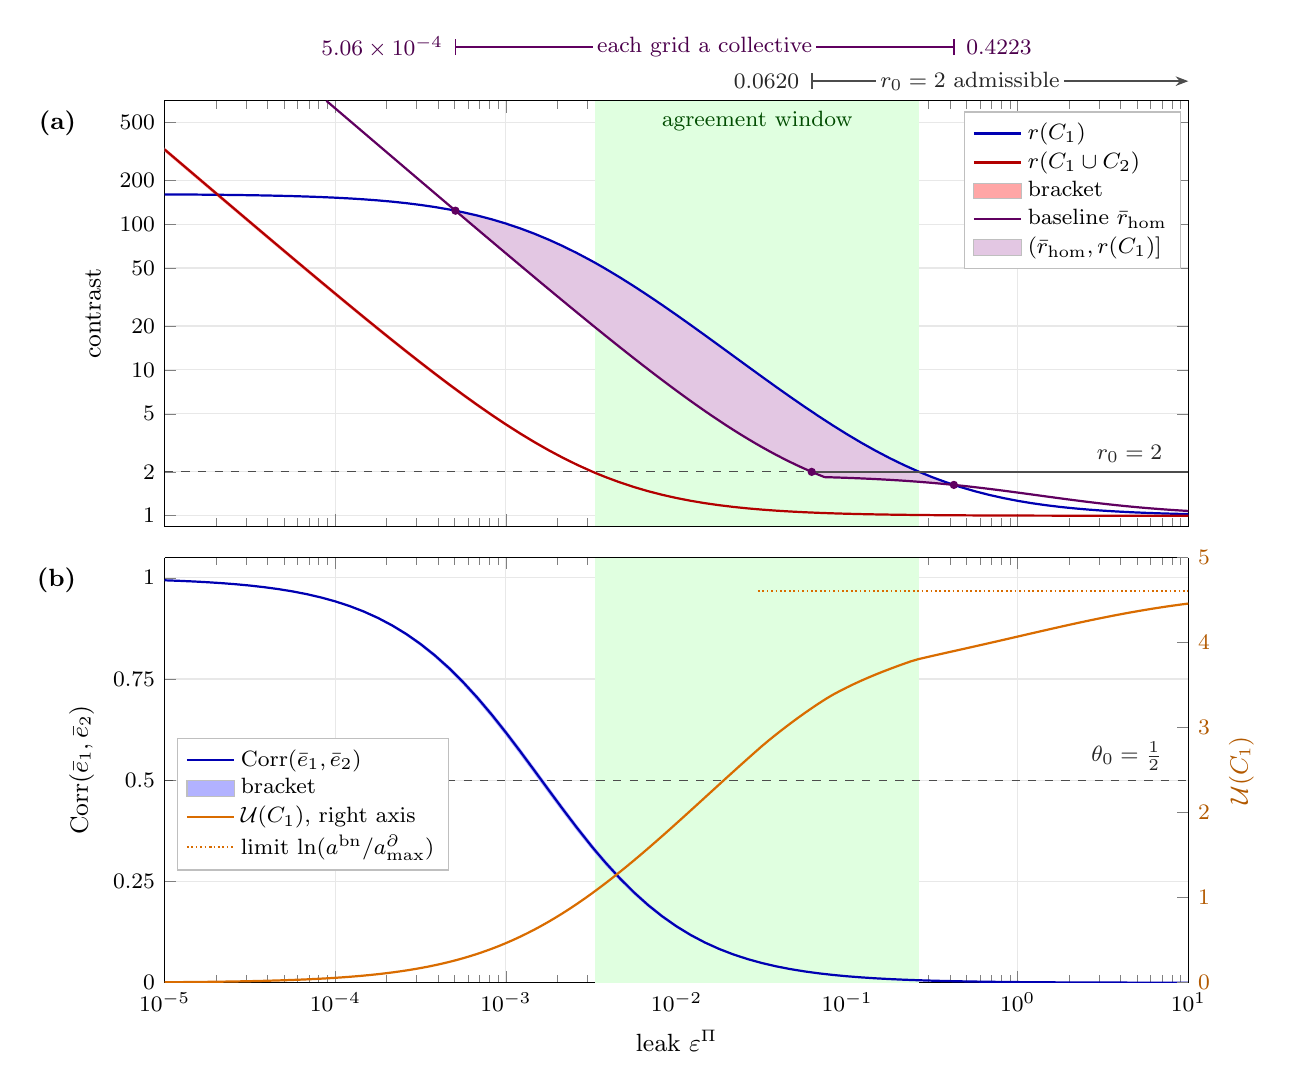
\begin{tikzpicture}
  \pgfplotsset{bridgeframe/.style={width=13cm, height=5.4cm, scale only axis, xmin=1e-5, xmax=10,
      xtick={1e-5,1e-4,1e-3,1e-2,1e-1,1,10},
      every axis label/.style={font=\small}, tick label style={font=\footnotesize},
      legend style={font=\footnotesize, draw=gray!50, fill=white, cells={anchor=west}, row sep=-1pt}}}
  % panel (a): spectral contrast
  \begin{axis}[bridgeframe, xmode=log, name=top, ymode=log, ymin=0.85, ymax=700,
      ytick={1,2,5,10,20,50,100,200,500}, log ticks with fixed point, xticklabels={},
      grid=major, grid style={gray!18}, ylabel={contrast},
      legend style={at={(0.993,0.975)}, anchor=north east}]
    \fill[green!12] (axis cs:0.0033333,0.85) rectangle (axis cs:0.264616,700);
    % levels at which each grid is a collective, between the baseline and r(C_1)
    \addplot[draw=none, fill=violet!22, forget plot] coordinates {(0.000505995,123.56) (0.000510897,123.28) (0.000562341,120.46) (0.000618966,117.5) (0.000681292,114.41) (0.000749894,111.19) (0.000825404,107.85) (0.000908518,104.4) (0.001,100.86) (0.00110069,97.223) (0.00121153,93.517) (0.00133352,89.755) (0.0014678,85.953) (0.0016156,82.128) (0.00177828,78.297) (0.00195734,74.477) (0.00215443,70.687) (0.00237137,66.944) (0.00261016,63.262) (0.00287298,59.657) (0.00316228,56.143) (0.00333333,54.257) (0.0034807,52.732) (0.00383119,49.434) (0.00421697,46.258) (0.00464159,43.212) (0.00510897,40.3) (0.00562341,37.527) (0.00618966,34.894) (0.00681292,32.403) (0.00749894,30.052) (0.00825404,27.841) (0.00908518,25.766) (0.01,23.824) (0.0110069,22.011) (0.0121153,20.321) (0.0133352,18.75) (0.014678,17.292) (0.016156,15.941) (0.0177828,14.691) (0.0195734,13.537) (0.0215443,12.472) (0.0237137,11.492) (0.0261016,10.589) (0.0287298,9.7603) (0.0316228,8.999) (0.034807,8.3007) (0.0383119,7.6606) (0.0421697,7.0745) (0.0464159,6.538) (0.0510897,6.0474) (0.0562341,5.5989) (0.0618966,5.1893) (0.062015,5.1815) (0.0681292,4.8152) (0.0737552,4.5306) (0.0749894,4.4737) (0.0825404,4.1622) (0.0908518,3.8782) (0.1,3.6192) (0.110069,3.3831) (0.121153,3.1681) (0.133352,2.9722) (0.14678,2.7938) (0.16156,2.6314) (0.177828,2.4835) (0.195734,2.3489) (0.215443,2.2265) (0.237137,2.1151) (0.261016,2.0137) (0.264616,2) (0.287298,1.9215) (0.316228,1.8376) (0.34807,1.7614) (0.383119,1.692) (0.421697,1.629) (0.422333,1.628) (0.422333,1.628) (0.421697,1.6283) (0.383119,1.6464) (0.34807,1.6638) (0.316228,1.6804) (0.287298,1.6963) (0.264616,1.7092) (0.261016,1.7113) (0.237137,1.7256) (0.215443,1.739) (0.195734,1.7517) (0.177828,1.7636) (0.16156,1.7747) (0.14678,1.7851) (0.133352,1.7948) (0.121153,1.8038) (0.110069,1.8122) (0.1,1.8199) (0.0908518,1.8271) (0.0825404,1.8337) (0.0749894,1.8398) (0.0737552,1.8408) (0.0681292,1.9103) (0.062015,2) (0.0618966,2.0019) (0.0562341,2.1028) (0.0510897,2.2138) (0.0464159,2.3361) (0.0421697,2.4706) (0.0383119,2.6187) (0.034807,2.7817) (0.0316228,2.9611) (0.0287298,3.1586) (0.0261016,3.3759) (0.0237137,3.6152) (0.0215443,3.8785) (0.0195734,4.1683) (0.0177828,4.4874) (0.016156,4.8385) (0.014678,5.225) (0.0133352,5.6505) (0.0121153,6.1187) (0.0110069,6.6342) (0.01,7.2015) (0.00908518,7.826) (0.00825404,8.5133) (0.00749894,9.2698) (0.00681292,10.103) (0.00618966,11.019) (0.00562341,12.028) (0.00510897,13.138) (0.00464159,14.361) (0.00421697,15.706) (0.00383119,17.187) (0.0034807,18.817) (0.00333333,19.604) (0.00316228,20.611) (0.00287298,22.586) (0.00261016,24.759) (0.00237137,27.152) (0.00215443,29.785) (0.00195734,32.683) (0.00177828,35.874) (0.0016156,39.385) (0.0014678,43.25) (0.00133352,47.505) (0.00121153,52.187) (0.00110069,57.342) (0.001,63.015) (0.000908518,69.26) (0.000825404,76.133) (0.000749894,83.698) (0.000681292,92.026) (0.000618966,101.19) (0.000562341,111.28) (0.000510897,122.38) (0.000505995,123.56)} -- cycle;
    \addplot[draw=none, fill=red!35, forget plot] coordinates {(1e-05,334.33) (1.2115e-05,276.13) (1.4678e-05,228.1) (1.7783e-05,188.45) (2.1544e-05,155.72) (2.6102e-05,128.71) (3.1623e-05,106.41) (3.8312e-05,88.005) (4.6416e-05,72.814) (5.6234e-05,60.276) (6.8129e-05,49.927) (8.254e-05,41.384) (0.0001,34.333) (0.00012115,28.513) (0.00014678,23.71) (0.00017783,19.745) (0.00021544,16.472) (0.00026102,13.771) (0.00031623,11.541) (0.00038312,9.7005) (0.00046416,8.1814) (0.00056234,6.9276) (0.00068129,5.8927) (0.0008254,5.0384) (0.001,4.3333) (0.0012115,3.7513) (0.0014678,3.271) (0.0017783,2.8745) (0.0021544,2.5472) (0.0026102,2.2771) (0.0031623,2.0541) (0.0033333,2) (0.0038312,1.8701) (0.0046416,1.7181) (0.0056234,1.5928) (0.0068129,1.4893) (0.008254,1.4038) (0.01,1.3333) (0.012115,1.2751) (0.014678,1.2271) (0.017783,1.1874) (0.021544,1.1547) (0.026102,1.1277) (0.031623,1.1054) (0.038312,1.087) (0.046416,1.0718) (0.056234,1.0593) (0.068129,1.0489) (0.08254,1.0404) (0.1,1.0333) (0.12115,1.0275) (0.14678,1.0227) (0.17783,1.0187) (0.21544,1.0155) (0.26102,1.0128) (0.26462,1.0126) (0.31623,1.0105) (0.38312,1.0087) (0.46416,1.0072) (0.56234,1.0059) (0.68129,1.0049) (0.8254,1.004) (1,1.0033) (1.2115,1.0028) (1.4678,1.0023) (1.7783,1.0019) (2.1544,1.0015) (2.6102,1.0013) (3.1623,1.0011) (3.8312,1.0009) (4.6416,1.0007) (5.6234,1.0006) (6.8129,1.0005) (8.254,1.0004) (10,1.0003) (10,1.0003) (8.254,1.0004) (6.8129,1.0005) (5.6234,1.0006) (4.6416,1.0007) (3.8312,1.0008) (3.1623,1.001) (2.6102,1.0012) (2.1544,1.0014) (1.7783,1.0018) (1.4678,1.0021) (1.2115,1.0026) (1,1.0031) (0.8254,1.0038) (0.68129,1.0046) (0.56234,1.0056) (0.46416,1.0067) (0.38312,1.0082) (0.31623,1.0099) (0.26462,1.0118) (0.26102,1.012) (0.21544,1.0145) (0.17783,1.0176) (0.14678,1.0213) (0.12115,1.0258) (0.1,1.0312) (0.08254,1.0378) (0.068129,1.0458) (0.056234,1.0555) (0.046416,1.0673) (0.038312,1.0815) (0.031623,1.0988) (0.026102,1.1197) (0.021544,1.145) (0.017783,1.1756) (0.014678,1.2128) (0.012115,1.2578) (0.01,1.3123) (0.008254,1.3784) (0.0068129,1.4585) (0.0056234,1.5554) (0.0046416,1.6729) (0.0038312,1.8153) (0.0033333,1.937) (0.0031623,1.9877) (0.0026102,2.1966) (0.0021544,2.4497) (0.0017783,2.7564) (0.0014678,3.1279) (0.0012115,3.5781) (0.001,4.1234) (0.0008254,4.7841) (0.00068129,5.5845) (0.00056234,6.5543) (0.00046416,7.7291) (0.00038312,9.1525) (0.00031623,10.877) (0.00026102,12.966) (0.00021544,15.497) (0.00017783,18.564) (0.00014678,22.279) (0.00012115,26.781) (0.0001,32.234) (8.254e-05,38.841) (6.8129e-05,46.845) (5.6234e-05,56.543) (4.6416e-05,68.291) (3.8312e-05,82.525) (3.1623e-05,99.77) (2.6102e-05,120.66) (2.1544e-05,145.97) (1.7783e-05,176.64) (1.4678e-05,213.79) (1.2115e-05,258.81) (1e-05,313.34)} -- cycle;
    \addplot[blue!70!black, thick] coordinates {(1e-05,159.82) (1.2115e-05,159.62) (1.4678e-05,159.37) (1.7783e-05,159.08) (2.1544e-05,158.73) (2.6102e-05,158.31) (3.1623e-05,157.79) (3.8312e-05,157.18) (4.6416e-05,156.44) (5.6234e-05,155.55) (6.8129e-05,154.5) (8.254e-05,153.23) (0.0001,151.73) (0.00012115,149.94) (0.00014678,147.84) (0.00017783,145.37) (0.00021544,142.48) (0.00026102,139.14) (0.00031623,135.29) (0.00038312,130.91) (0.00046416,125.97) (0.00056234,120.46) (0.00068129,114.41) (0.0008254,107.85) (0.001,100.86) (0.0012115,93.517) (0.0014678,85.953) (0.0017783,78.297) (0.0021544,70.687) (0.0026102,63.262) (0.0031623,56.143) (0.0033333,54.257) (0.0038312,49.434) (0.0046416,43.212) (0.0056234,37.527) (0.0068129,32.403) (0.008254,27.841) (0.01,23.824) (0.012115,20.321) (0.014678,17.292) (0.017783,14.691) (0.021544,12.472) (0.026102,10.589) (0.031623,8.999) (0.038312,7.6606) (0.046416,6.538) (0.056234,5.5989) (0.068129,4.8152) (0.08254,4.1622) (0.1,3.6192) (0.12115,3.1681) (0.14678,2.7938) (0.17783,2.4835) (0.21544,2.2265) (0.26102,2.0137) (0.26462,2) (0.31623,1.8376) (0.38312,1.692) (0.46416,1.5716) (0.56234,1.4721) (0.68129,1.3899) (0.8254,1.322) (1,1.2658) (1.2115,1.2195) (1.4678,1.1812) (1.7783,1.1496) (2.1544,1.1235) (2.6102,1.102) (3.1623,1.0842) (3.8312,1.0695) (4.6416,1.0573) (5.6234,1.0473) (6.8129,1.0391) (8.254,1.0323) (10,1.0266)};
    \addlegendentry{$r(C_1)$}
    \addplot[red!70!black, thick] coordinates {(1e-05,324.36) (1.2115e-05,267.9) (1.4678e-05,221.3) (1.7783e-05,182.84) (2.1544e-05,151.09) (2.6102e-05,124.88) (3.1623e-05,103.25) (3.8312e-05,85.401) (4.6416e-05,70.665) (5.6234e-05,58.502) (6.8129e-05,48.462) (8.254e-05,40.175) (0.0001,33.336) (0.00012115,27.69) (0.00014678,23.03) (0.00017783,19.184) (0.00021544,16.009) (0.00026102,13.388) (0.00031623,11.225) (0.00038312,9.4401) (0.00046416,7.9665) (0.00056234,6.7502) (0.00068129,5.7462) (0.0008254,4.9175) (0.001,4.2336) (0.0012115,3.669) (0.0014678,3.203) (0.0017783,2.8184) (0.0021544,2.5009) (0.0026102,2.2388) (0.0031623,2.0225) (0.0033333,1.9701) (0.0038312,1.844) (0.0046416,1.6966) (0.0056234,1.575) (0.0068129,1.4746) (0.008254,1.3918) (0.01,1.3234) (0.012115,1.2669) (0.014678,1.2203) (0.017783,1.1818) (0.021544,1.1501) (0.026102,1.1239) (0.031623,1.1023) (0.038312,1.0844) (0.046416,1.0697) (0.056234,1.0575) (0.068129,1.0475) (0.08254,1.0392) (0.1,1.0323) (0.12115,1.0267) (0.14678,1.022) (0.17783,1.0182) (0.21544,1.015) (0.26102,1.0124) (0.26462,1.0122) (0.31623,1.0102) (0.38312,1.0084) (0.46416,1.007) (0.56234,1.0058) (0.68129,1.0047) (0.8254,1.0039) (1,1.0032) (1.2115,1.0027) (1.4678,1.0022) (1.7783,1.0018) (2.1544,1.0015) (2.6102,1.0012) (3.1623,1.001) (3.8312,1.0008) (4.6416,1.0007) (5.6234,1.0006) (6.8129,1.0005) (8.254,1.0004) (10,1.0003)};
    \addlegendentry{$r(C_1\cup C_2)$}
    \addlegendimage{area legend, draw=none, fill=red!35}
    \addlegendentry{bracket}
    \addplot[violet!75!black, thick] coordinates {(8.87196e-05,700) (9.08518e-05,683.6) (0.0001,621.15) (0.000110069,564.42) (0.000121153,512.87) (0.000133352,466.05) (0.00014678,423.5) (0.00016156,384.85) (0.000177828,349.74) (0.000195734,317.83) (0.000215443,288.85) (0.000237137,262.52) (0.000261016,238.59) (0.000287298,216.86) (0.000316228,197.11) (0.00034807,179.17) (0.000383119,162.87) (0.000421697,148.06) (0.000464159,134.61) (0.000505995,123.56) (0.000510897,122.38) (0.000562341,111.28) (0.000618966,101.19) (0.000681292,92.026) (0.000749894,83.698) (0.000825404,76.133) (0.000908518,69.26) (0.001,63.015) (0.00110069,57.342) (0.00121153,52.187) (0.00133352,47.505) (0.0014678,43.25) (0.0016156,39.385) (0.00177828,35.874) (0.00195734,32.683) (0.00215443,29.785) (0.00237137,27.152) (0.00261016,24.759) (0.00287298,22.586) (0.00316228,20.611) (0.00333333,19.604) (0.0034807,18.817) (0.00383119,17.187) (0.00421697,15.706) (0.00464159,14.361) (0.00510897,13.138) (0.00562341,12.028) (0.00618966,11.019) (0.00681292,10.103) (0.00749894,9.2698) (0.00825404,8.5133) (0.00908518,7.826) (0.01,7.2015) (0.0110069,6.6342) (0.0121153,6.1187) (0.0133352,5.6505) (0.014678,5.225) (0.016156,4.8385) (0.0177828,4.4874) (0.0195734,4.1683) (0.0215443,3.8785) (0.0237137,3.6152) (0.0261016,3.3759) (0.0287298,3.1586) (0.0316228,2.9611) (0.034807,2.7817) (0.0383119,2.6187) (0.0421697,2.4706) (0.0464159,2.3361) (0.0510897,2.2138) (0.0562341,2.1028) (0.0618966,2.0019) (0.062015,2) (0.0681292,1.9103) (0.0737552,1.8408) (0.0749894,1.8398) (0.0825404,1.8337) (0.0908518,1.8271) (0.1,1.8199) (0.110069,1.8122) (0.121153,1.8038) (0.133352,1.7948) (0.14678,1.7851) (0.16156,1.7747) (0.177828,1.7636) (0.195734,1.7517) (0.215443,1.739) (0.237137,1.7256) (0.261016,1.7113) (0.264616,1.7092) (0.287298,1.6963) (0.316228,1.6804) (0.34807,1.6638) (0.383119,1.6464) (0.421697,1.6283) (0.422333,1.628) (0.464159,1.6095) (0.510897,1.5901) (0.562341,1.5701) (0.618966,1.5496) (0.681292,1.5286) (0.749894,1.5074) (0.825404,1.4858) (0.908518,1.4642) (1,1.4425) (1.10069,1.4208) (1.21153,1.3993) (1.33352,1.378) (1.4678,1.357) (1.6156,1.3365) (1.77828,1.3165) (1.95734,1.297) (2.15443,1.2782) (2.37137,1.26) (2.61016,1.2426) (2.87298,1.226) (3.16228,1.2101) (3.4807,1.195) (3.83119,1.1807) (4.21697,1.1672) (4.64159,1.1546) (5.10897,1.1426) (5.62341,1.1315) (6.18966,1.1211) (6.81292,1.1114) (7.49894,1.1023) (8.25404,1.0939) (9.08518,1.0862) (10,1.079)};
    \addlegendentry{baseline $\bar r_{\mathrm{hom}}$}
    \addlegendimage{area legend, draw=none, fill=violet!22}
    \addlegendentry{$(\bar r_{\mathrm{hom}},r(C_1)]$}
    \draw[gray!60!black, dashed] (axis cs:1e-5,2) -- (axis cs:10,2);
    % the level r_0 = 2 is admissible where it lies above the baseline
    \draw[gray!60!black, thick] (axis cs:0.062015,2) -- (axis cs:10,2);
    \fill[violet!75!black] (axis cs:0.062015,2) circle (1.5pt);
    \fill[violet!75!black] (axis cs:5.05995e-4,123.56) circle (1.5pt);
    \fill[violet!75!black] (axis cs:0.422333,1.628) circle (1.5pt);
    \coordinate (bLo) at (axis cs:5.05995e-4,700);
    \coordinate (bHi) at (axis cs:0.422333,700);
    \coordinate (bAdm) at (axis cs:0.062015,700);
    \coordinate (bEnd) at (axis cs:10,700);
    \node[font=\footnotesize, gray!30!black, anchor=south east] at (axis cs:8,2) {$r_0=2$};
    \node[font=\footnotesize, green!30!black, anchor=north] at (axis cs:0.02970,700) {agreement window};
  \end{axis}
  \node[font=\small\bfseries, anchor=north east] at ([xshift=-1.0cm]top.north west) {(a)};
  % leak ranges on the leak axis of panel (a): each grid a collective at some admissible level, and r_0 = 2 admissible
  \begin{scope}[font=\footnotesize]
    \draw[violet!75!black, semithick] ([yshift=0.68cm]bLo) -- ([yshift=0.68cm]bHi)
      node[pos=0.5, fill=white, inner sep=1.5pt, text=violet!60!black] {each grid a collective};
    \draw[violet!75!black, semithick] ([yshift=0.58cm]bLo) -- ([yshift=0.78cm]bLo);
    \draw[violet!75!black, semithick] ([yshift=0.58cm]bHi) -- ([yshift=0.78cm]bHi);
    \node[text=violet!60!black, anchor=east] at ([xshift=-1pt, yshift=0.68cm]bLo) {$5.06\times10^{-4}$};
    \node[text=violet!60!black, anchor=west] at ([xshift=1pt, yshift=0.68cm]bHi) {$0.4223$};
    \draw[gray!60!black, thick, -{Stealth[length=1.6mm]}] ([yshift=0.25cm]bAdm) -- ([yshift=0.25cm]bEnd)
      node[pos=0.42, fill=white, inner sep=1.5pt, text=gray!30!black] {$r_0=2$ admissible};
    \draw[gray!60!black, thick] ([yshift=0.15cm]bAdm) -- ([yshift=0.35cm]bAdm);
    \node[text=gray!30!black, anchor=east] at ([xshift=-1pt, yshift=0.25cm]bAdm) {$0.0620$};
  \end{scope}
  % panel (b): correlation of the block averages (left) and ultrametric contrast (right)
  \begin{axis}[bridgeframe, xmode=log, name=bot, at={($(top.south west)+(0,-0.4cm)$)}, anchor=north west,
      ymin=0, ymax=1.05, ytick={0,0.25,0.5,0.75,1}, axis y line*=left,
      grid=major, grid style={gray!18}, xlabel={leak $\varepsilon^\Pi$},
      ylabel={$\Corr(\bar e_1,\bar e_2)$},
      legend style={at={(0.012,0.42)}, anchor=west}]
    \fill[green!12] (axis cs:0.0033333,0) rectangle (axis cs:0.264616,1.05);
    \addplot[draw=none, fill=blue!30, forget plot] coordinates {(1e-05,0.99404) (1.2115e-05,0.99278) (1.4678e-05,0.99127) (1.7783e-05,0.98944) (2.1544e-05,0.98724) (2.6102e-05,0.98458) (3.1623e-05,0.98138) (3.8312e-05,0.97753) (4.6416e-05,0.97291) (5.6234e-05,0.96736) (6.8129e-05,0.96073) (8.254e-05,0.95281) (0.0001,0.9434) (0.00012115,0.93223) (0.00014678,0.91906) (0.00017783,0.90359) (0.00021544,0.88553) (0.00026102,0.8646) (0.00031623,0.84052) (0.00038312,0.81309) (0.00046416,0.78217) (0.00056234,0.74772) (0.00068129,0.70984) (0.0008254,0.66879) (0.001,0.625) (0.0012115,0.57907) (0.0014678,0.53172) (0.0017783,0.4838) (0.0021544,0.43617) (0.0026102,0.3897) (0.0031623,0.34514) (0.0033333,0.33333) (0.0038312,0.30315) (0.0046416,0.2642) (0.0056234,0.22862) (0.0068129,0.19655) (0.008254,0.168) (0.01,0.14286) (0.012115,0.12093) (0.014678,0.10197) (0.017783,0.085692) (0.021544,0.071805) (0.026102,0.060021) (0.031623,0.050066) (0.038312,0.041689) (0.046416,0.034663) (0.056234,0.028785) (0.068129,0.023879) (0.08254,0.019792) (0.1,0.016393) (0.12115,0.01357) (0.14678,0.011227) (0.17783,0.0092853) (0.21544,0.0076766) (0.26102,0.0063448) (0.26462,0.006259) (0.31623,0.0052428) (0.38312,0.0043314) (0.46416,0.0035779) (0.56234,0.002955) (0.68129,0.0024404) (0.8254,0.0020151) (1,0.0016639) (1.2115,0.0013738) (1.4678,0.0011342) (1.7783,0.00093636) (2.1544,0.000773) (2.6102,0.00063812) (3.1623,0.00052677) (3.8312,0.00043484) (4.6416,0.00035894) (5.6234,0.00029629) (6.8129,0.00024457) (8.254,0.00020188) (10,0.00016664) (10,0.00016637) (8.254,0.00020149) (6.8129,0.000244) (5.6234,0.00029545) (4.6416,0.00035773) (3.8312,0.00043307) (3.1623,0.00052421) (2.6102,0.00063443) (2.1544,0.00076769) (1.7783,0.00092874) (1.4678,0.0011233) (1.2115,0.0013583) (1,0.0016421) (0.8254,0.0019845) (0.68129,0.0023976) (0.56234,0.0028959) (0.46416,0.0034967) (0.38312,0.004221) (0.31623,0.005094) (0.26462,0.0060643) (0.26102,0.0061461) (0.21544,0.0074139) (0.17783,0.0089413) (0.14678,0.010781) (0.12115,0.012996) (0.1,0.015663) (0.08254,0.018869) (0.068129,0.022722) (0.056234,0.027345) (0.046416,0.032885) (0.038312,0.03951) (0.031623,0.047413) (0.026102,0.056812) (0.021544,0.067952) (0.017783,0.081099) (0.014678,0.096537) (0.012115,0.11456) (0.01,0.13545) (0.008254,0.15948) (0.0068129,0.18686) (0.0056234,0.21773) (0.0046416,0.25212) (0.0038312,0.28995) (0.0033333,0.3194) (0.0031623,0.33095) (0.0026102,0.37469) (0.0021544,0.42058) (0.0017783,0.46789) (0.0014678,0.5158) (0.0012115,0.56341) (0.001,0.60989) (0.0008254,0.65446) (0.00068129,0.69647) (0.00056234,0.73544) (0.00046416,0.77105) (0.00038312,0.80315) (0.00031623,0.83174) (0.00026102,0.85691) (0.00021544,0.87886) (0.00017783,0.89785) (0.00014678,0.91416) (0.00012115,0.92807) (0.0001,0.93987) (8.254e-05,0.94984) (6.8129e-05,0.95823) (5.6234e-05,0.96527) (4.6416e-05,0.97116) (3.8312e-05,0.97607) (3.1623e-05,0.98017) (2.6102e-05,0.98357) (2.1544e-05,0.9864) (1.7783e-05,0.98875) (1.4678e-05,0.9907) (1.2115e-05,0.99231) (1e-05,0.99364)} -- cycle;
    \addplot[blue!70!black, thick] coordinates {(1e-05,0.99385) (1.2115e-05,0.99256) (1.4678e-05,0.99101) (1.7783e-05,0.98912) (2.1544e-05,0.98685) (2.6102e-05,0.98412) (3.1623e-05,0.98082) (3.8312e-05,0.97686) (4.6416e-05,0.9721) (5.6234e-05,0.9664) (6.8129e-05,0.95958) (8.254e-05,0.95144) (0.0001,0.94177) (0.00012115,0.93031) (0.00014678,0.91679) (0.00017783,0.90094) (0.00021544,0.88245) (0.00026102,0.86104) (0.00031623,0.83645) (0.00038312,0.80848) (0.00046416,0.77701) (0.00056234,0.74201) (0.00068129,0.70361) (0.0008254,0.6621) (0.001,0.61794) (0.0012115,0.57174) (0.0014678,0.52425) (0.0017783,0.47633) (0.0021544,0.42883) (0.0026102,0.38262) (0.0031623,0.33843) (0.0033333,0.32674) (0.0038312,0.2969) (0.0046416,0.25847) (0.0056234,0.22344) (0.0068129,0.19193) (0.008254,0.16393) (0.01,0.13932) (0.012115,0.11788) (0.014678,0.099359) (0.017783,0.083478) (0.021544,0.069942) (0.026102,0.058463) (0.031623,0.048772) (0.038312,0.040621) (0.046416,0.033787) (0.056234,0.02807) (0.068129,0.0233) (0.08254,0.019326) (0.1,0.01602) (0.12115,0.013273) (0.14678,0.010993) (0.17783,0.0091017) (0.21544,0.0075337) (0.26102,0.0062344) (0.26462,0.0061507) (0.31623,0.0051582) (0.38312,0.004267) (0.46416,0.0035292) (0.56234,0.0029185) (0.68129,0.0024131) (0.8254,0.001995) (1,0.001649) (1.2115,0.0013629) (1.4678,0.0011263) (1.7783,0.00093064) (2.1544,0.00076889) (2.6102,0.00063518) (3.1623,0.00052467) (3.8312,0.00043335) (4.6416,0.0003579) (5.6234,0.00029556) (6.8129,0.00024406) (8.254,0.00020152) (10,0.00016639)};
    \addlegendentry{$\Corr(\bar e_1,\bar e_2)$}
    \addlegendimage{area legend, draw=none, fill=blue!30}
    \addlegendentry{bracket}
    \addlegendimage{orange!85!black, thick}
    \addlegendentry{$\mathcal U(C_1)$, right axis}
    \addlegendimage{orange!85!black, densely dotted, semithick}
    \addlegendentry{limit $\ln(a^{\mathrm{bn}}/a^\partial_{\max})$}
    \draw[gray!60!black, dashed] (axis cs:1e-5,0.5) -- (axis cs:10,0.5);
    \node[font=\footnotesize, gray!30!black, anchor=south east] at (axis cs:8,0.5) {$\theta_0=\frac12$};
  \end{axis}
  \begin{axis}[bridgeframe, xmode=log, at={(bot.south west)}, anchor=south west,
      ymin=0, ymax=5, ytick={0,1,2,3,4,5}, axis y line*=right, axis x line=none,
      ylabel={$\mathcal U(C_1)$}, ylabel style={orange!70!black},
      y tick label style={orange!70!black}]
    \addplot[orange!85!black, thick] coordinates {(1e-05,0.005972) (1.1007e-05,0.0065713) (1.2115e-05,0.0072306) (1.3335e-05,0.0079557) (1.4678e-05,0.0087532) (1.6156e-05,0.0096302) (1.7783e-05,0.010595) (1.9573e-05,0.011655) (2.1544e-05,0.012821) (2.3714e-05,0.014103) (2.6102e-05,0.015512) (2.873e-05,0.01706) (3.1623e-05,0.018761) (3.4807e-05,0.020631) (3.8312e-05,0.022684) (4.217e-05,0.024939) (4.6416e-05,0.027415) (5.109e-05,0.030134) (5.6234e-05,0.033117) (6.1897e-05,0.03639) (6.8129e-05,0.03998) (7.4989e-05,0.043916) (8.254e-05,0.048231) (9.0852e-05,0.052957) (0.0001,0.058134) (0.00011007,0.063799) (0.00012115,0.069998) (0.00013335,0.076775) (0.00014678,0.08418) (0.00016156,0.092266) (0.00017783,0.10109) (0.00019573,0.11071) (0.00021544,0.12118) (0.00023714,0.13259) (0.00026102,0.14498) (0.0002873,0.15845) (0.00031623,0.17305) (0.00034807,0.18888) (0.00038312,0.206) (0.0004217,0.2245) (0.00046416,0.24447) (0.0005109,0.26597) (0.00056234,0.2891) (0.00061897,0.31393) (0.00068129,0.34054) (0.00074989,0.369) (0.0008254,0.39938) (0.00090852,0.43174) (0.001,0.46614) (0.0011007,0.50262) (0.0012115,0.54122) (0.0013335,0.58198) (0.0014678,0.6249) (0.0016156,0.67) (0.0017783,0.71728) (0.0019573,0.76671) (0.0021544,0.81828) (0.0023714,0.87194) (0.0026102,0.92764) (0.002873,0.98533) (0.0031623,1.0449) (0.0034807,1.1064) (0.0038312,1.1696) (0.004217,1.2344) (0.0046416,1.3009) (0.005109,1.3687) (0.0056234,1.438) (0.0061897,1.5084) (0.0068129,1.58) (0.0074989,1.6526) (0.008254,1.7261) (0.0090852,1.8003) (0.01,1.8752) (0.011007,1.9506) (0.012115,2.0264) (0.013335,2.1025) (0.014678,2.1788) (0.016156,2.2552) (0.017783,2.3315) (0.019573,2.4076) (0.021544,2.4834) (0.023714,2.5589) (0.026102,2.6338) (0.02873,2.7081) (0.031623,2.7817) (0.034807,2.8519) (0.038312,2.919) (0.04217,2.9844) (0.046416,3.0481) (0.05109,3.1099) (0.056234,3.1698) (0.061897,3.2277) (0.068129,3.2836) (0.074989,3.3375) (0.08254,3.3874) (0.090852,3.4319) (0.1,3.4742) (0.11007,3.5145) (0.12115,3.5528) (0.13335,3.5893) (0.14678,3.6243) (0.16156,3.6577) (0.17783,3.6899) (0.19573,3.721) (0.21544,3.7512) (0.23714,3.7805) (0.26102,3.8051) (0.2873,3.8246) (0.31623,3.8438) (0.34807,3.8627) (0.38312,3.8815) (0.4217,3.9002) (0.46416,3.9189) (0.5109,3.9376) (0.56234,3.9564) (0.61897,3.9753) (0.68129,3.9943) (0.74989,4.0134) (0.8254,4.0325) (0.90852,4.0518) (1,4.0711) (1.1007,4.0904) (1.2115,4.1097) (1.3335,4.1289) (1.4678,4.148) (1.6156,4.167) (1.7783,4.1859) (1.9573,4.2045) (2.1544,4.2229) (2.3714,4.2409) (2.6102,4.2587) (2.873,4.2761) (3.1623,4.2931) (3.4807,4.3098) (3.8312,4.3259) (4.217,4.3416) (4.6416,4.3568) (5.109,4.3715) (5.6234,4.3857) (6.1897,4.3993) (6.8129,4.4124) (7.4989,4.425) (8.254,4.4369) (9.0852,4.4484) (10,4.4592)};
    \draw[orange!85!black, densely dotted, semithick] (axis cs:0.03,4.60517) -- (axis cs:10,4.60517);
  \end{axis}
  \node[font=\small\bfseries, anchor=north east] at ([xshift=-1.0cm]bot.north west) {(b)};
\end{tikzpicture}

  \caption{\textbf{Spectral and correlation criteria against the leak.} The two $6\times6$ grids of \cref{tab:col-bridge} under a uniform leak $\varepsilon^\Pi$. (a) The block contrast $r(C_1)$ and the union contrast $r(C_1\cup C_2)$ with its bracket \eqref{eq:col-union}, against the level $r_0=2$ and the baseline $\bar r_{\mathrm{hom}}$ of the population declared on its $6\times12$ box, the larger of $1+0.0620/\varepsilon^\Pi$ and $(\varepsilon^\Pi+1.82)/(\varepsilon^\Pi+0.955)$ (\cref{obs:col-bridge-baseline}). (b) The correlation of the block averages with its bracket \eqref{eq:col-corr}, against $\theta_0=\frac12$, and the ultrametric contrast $\mathcal U(C_1)$ of \cref{def:col-ultrametric} (right axis), with its strong-grounding limit $\ln(a^{\mathrm{bn}}/a^\partial_{\max})=\ln100$. The shaded column is the window \eqref{eq:col-window}, $0.0033<\varepsilon^\Pi\le0.2646$, on which both criteria return the two grids and not their union. Left of it the criterion $r\ge r_0$ also returns the union, up to $\varepsilon^\Pi=\lambda_2(L^\Pi)=0.003234$, while the block averages are correlated above $\theta_0$ only below $\varepsilon^\Pi=0.001617$; right of it the criterion returns nothing, the block averages are nearly uncorrelated and $\mathcal U(C_1)$ approaches its limit. The level $r_0=2$ is admissible only for $\varepsilon^\Pi>0.0620$, where the baseline falls below it (lower bar, dot and solid part of the level line), and lies below the baseline wherever the union is returned. Each grid is a collective for $5.06\times10^{-4}<\varepsilon^\Pi<0.4223$ (upper bar and dots), at the levels between the baseline and $r(C_1)$ (violet band); the union, the whole closed population, is a collective at no leak. The brackets are tight, of relative width at most $6.5$ percent for the union contrast and width at most $0.016$ for the correlation (\cref{chk:col-bridge}).}
  \label{fig:col-bridge}
\end{figure}

For the two-grid population of \cref{tab:col-bridge}, declared on its box of $\Z^2$ or as its nearest-neighbor graph, the baseline is the larger of the contrasts of the whole comparison box and of a $2\times2$ square at its corner, and each grid is a collective at some admissible level exactly for $5.060\times10^{-4}<\varepsilon^\Pi<0.4223$ under the lattice clause, with largest significance $3.32$ (Supplement, a numerical observation, \cref{obs:col-bridge-baseline}).

The criterion $r\ge r_0$ is hierarchical: at weak grounding it returns each block and also their union, and which returned sets are collectives is decided by the baseline. For the two grids at $r_0=2$ the union is a collective at no leak, and the spectral and the correlation criteria agree only when grounding lies between the cut coupling per member and the internal stiffness (Supplement, \cref{rem:col-bridge-reading}).

Explicit two-sided bounds of the form \eqref{eq:col-union} and \eqref{eq:col-corr} for unequal blocks, for more than two blocks and for blocks coupled to an exterior are open (Supplement, \cref{open:col-bridge}).

Contrast is a statement about relaxation rates, while H1 speaks of coherence, and up to a dependence on dimension the members of a contrasted region are coherent with its average. With uniform leak the mean correlation of the members with the average, weighted by their standard deviations, is at least $(r(C)/(r(C)+n-1))^{1/2}$, and for an isolated interval with nearest-neighbor coupling at contrast $r$ the mean inverse squared correlation is below $1+\pi^2/(6(r-1))$ at every size; in a numerical observation on isolated boxes at fixed contrast the same quantity grows with the side, logarithmically in two dimensions and linearly in three (Supplement, \cref{sec:col-coherence}, \cref{prop:col-coherence-average,obs:col-coherence-dimension}).

\subsection{Nested and multiplex collectives}\label{sec:col-nested}

Collectives nest within a modality and overlap across modalities (\cref{asm:int-a9}). Both statements have exact forms for blankets and for the ultrametric classes of \cref{def:col-ultrametric}. For spectral contrast, nesting is a matter of baselines, and it takes two forms: nesting within one medium, in which every set of the nest exceeds the same baseline, and nesting across levels, in which collectives of collectives are judged in coarse media of their own. The exact law of block averages is in general not diffusive (\cref{ex:ren-block-average}), so the coarse media are built from the precision itself.

\begin{definition}[Coarse medium]\label{def:col-coarse-medium}
Let $\Pi=\diag(\varepsilon^\Pi)+L^\Pi$ be a diffusive positive definite precision on a finite population $V$, let $\mathcal P=\{C_1,\dots,C_M\}$ be a partition of $V$ into nonempty blocks, and let $\mathsf P\in\{0,1\}^{M\times V}$ be the matrix whose rows are the block indicators $\one_{C_\alpha}^\top$. The coarse medium of $\mathcal P$ is the Galerkin precision
\begin{equation}\label{eq:col-coarse-medium}
\Pi^{\mathcal P}=\mathsf P\Pi\mathsf P^\top,\qquad\Pi^{\mathcal P}_{\alpha\beta}=\sum_{i\in C_\alpha}\sum_{j\in C_\beta}\Pi_{ij},
\end{equation}
on the blocks as units. Its off-diagonal entries are $-\cut(C_\alpha,C_\beta)$, with $\cut(C_\alpha,C_\beta)=\sum_{i\in C_\alpha,j\in C_\beta}a^\Pi_{ij}$, and its row sums are the block sums $\sum_{i\in C_\alpha}\varepsilon^\Pi_i$ of the leaks. For a chain of partitions $\mathcal P_0\prec\mathcal P_1\prec\dots\prec\mathcal P_{l_{\max}}$, in which every block of $\mathcal P_{l+1}$ is a union of blocks of $\mathcal P_l$ and $\mathcal P_0$ is the partition into single agents, the level-$l$ coarse medium is $\Pi^{(l)}=\mathsf P_l\Pi\mathsf P_l^\top$, and the coarse contrast $r^{(l)}(S)$ of a set $S$ of blocks of $\mathcal P_l$ is the contrast of \cref{def:col-contrast} computed from $\Pi^{(l)}$. The geometry of each coarse medium is declared with the model.
\end{definition}
% src: H6-D2, M_spec_H5 Section 4 (block-sum convention, assumption A3 of H6)

\begin{lemma}[Properties of the coarse medium]\label{lem:col-coarse-medium}
In the setting of \cref{def:col-coarse-medium}, let $n_\alpha=|C_\alpha|$, let $\Phi=\mathsf P^\top\diag(n_\alpha)^{-1/2}$ be the block frame of \cref{thm:col-bridge}, and let $\Phi_\perp$ be an orthonormal basis of the orthogonal complement of its span.
\begin{enumerate}
\item[(a)] $\Pi^{\mathcal P}$ is diffusive and positive definite, with couplings $\cut(C_\alpha,C_\beta)$ and leaks $\sum_{i\in C_\alpha}\varepsilon^\Pi_i$.
\item[(b)] Let $e\sim\Ncal(0,\Pi^{-1})$ and let $\bar e=\diag(n_\alpha)^{-1}\mathsf Pe$ be the vector of block averages. Given $\Phi_\perp^\top e=0$, that is, given that every block is in exact internal agreement, $\bar e$ has precision $\Pi^{\mathcal P}$. Without conditioning $\bar e$ has precision $\Pi^{\mathcal P}-\diag(n_\alpha)^{1/2}\mathcal D\diag(n_\alpha)^{1/2}$, with $\mathcal D=\Phi^\top\Pi\Phi_\perp(\Phi_\perp^\top\Pi\Phi_\perp)^{-1}\Phi_\perp^\top\Pi\Phi\succeq0$ as in \cref{thm:col-bridge}(ii), and this equals $\Pi^{\mathcal P}$ if and only if $\Pi$ maps the span of the block indicators into itself; for uniform leak this is the equitable condition of \cref{thm:col-bridge}(ii).
\item[(c)] Coarse media compose: if $\mathsf Q_l$ is the indicator matrix of $\mathcal P_{l+1}$ as a partition of the blocks of $\mathcal P_l$, then $\mathsf P_{l+1}=\mathsf Q_l\mathsf P_l$ and $\Pi^{(l+1)}=\mathsf Q_l\Pi^{(l)}\mathsf Q_l^\top$.
\item[(d)] For blocks of equal size $s$, $\Pi^{\mathcal P}=s\Phi^\top\Pi\Phi$, so coarse contrasts equal those of the orthonormal block precision $\Phi^\top\Pi\Phi$; for blocks of unequal sizes the two in general differ, and $\Phi^\top\Pi\Phi$ need not be diffusive.
\end{enumerate}
\end{lemma}
% src: H6-L1 (with the conditional reading of (b) added here)
Proof in \cref{app:col}; checked in \cref{chk:col-coarse-medium}. Part (b) explains the name: the coarse medium is the law of the block values when every block is held in exact internal agreement, and it differs from the law of the block averages by the correction of \cref{thm:col-bridge}(ii), which with uniform leak vanishes exactly for equitable partitions and is bounded entrywise by $\sigma_X\sigma_Y/\varkappa_\perp$ otherwise, with $\sigma_X$ the equitability defect of block $X$ and $\varkappa_\perp$ the smallest eigenvalue of the precision on the complement of the block indicators, small when the internal stiffness is large against the dispersion of the cut (\cref{lem:ren-galerkin}). Part (d) fixes a convention that matters for unequal blocks; we use block sums throughout, which by (a) keep the coarse medium diffusive.

\begin{definition}[Hierarchy of collectives]\label{def:col-hierarchy}
A hierarchy of collectives consists of a chain of partitions $\mathcal P_0\prec\mathcal P_1\prec\dots\prec\mathcal P_{l_{\max}}$ of a finite population, declared with the model, with $\mathcal P_0$ the partition into single agents; a declared geometry and a declared level $r^{(l)}_0$ for each coarse medium $\Pi^{(l)}$, $0\le l<l_{\max}$; and, for each $l\ge1$, a declared family $\mathfrak C_l\subseteq\mathcal P_l$ of blocks such that every $C\in\mathfrak C_l$, viewed as the set of blocks of $\mathcal P_{l-1}$ that it contains, is a collective at level $r^{(l-1)}_0$ in the sense of \cref{def:col-collective}, with $\Pi^{(l-1)}$ in place of the world-conditional precision and the comparison medium of $\Pi^{(l-1)}$ with its declared geometry. The blocks of $\mathfrak C_l$ are the collectives of level $l$, each a candidate meta-agent of that level.
\end{definition}
% src: H6-D3 (with level-specific declared levels, assumption A4 of H6, shown necessary by H6-T2(e) and obs:col-nested-medium)
A hierarchy is judged level by level. Levels are declared separately because the baselines of different coarse media can be far apart, so that no single level serves a whole hierarchy (\cref{obs:col-nested-medium}); the nested medium without declared geometry is judged level by level in \cref{prop:ren-per-level}. Whether a collective of level $l$ is also a collective of the fine medium is a separate question, answered by the fine baseline.

\begin{definition}[Nested and multiplex collectives]\label{def:col-nested}
A nested collective of depth two in one medium is a collective $C$ at level $r_0$, with its canonical partition, together with disjoint collectives $C_1,\dots,C_M\subseteq C$, $M\ge2$, at the same level, with theirs, all judged in the same medium against the same baseline; deeper nesting in one medium is defined recursively, and the nesting is exact at a level when every canonical partition of that level is an exact path blanket. Nesting across levels, in which each level is judged in its own coarse medium against that medium's comparison medium, is a hierarchy of collectives (\cref{def:col-hierarchy}). In a multiplex population every channel carries one modality $c\in\mathcal M$, and an agent's internal state may decompose as $\mu_i=(\mu_i^{(c)})_{c\in\mathcal M}$. A modality-$c$ collective uses the modality-restricted partition, in which only modality-$c$ member channels that read or drive non-members are blanket variables. Its split partition also treats the internal coordinates $\mu_i^{(c')}$, $c'\neq c$, and the channels of other modalities of every member as exterior.
\end{definition}
% src: L2-D5, L2-D6, L5-D5; nesting within one medium distinguished from nesting across levels per H6-D3 (decision 22)

Blankets nest, the ultrametric classes of one modality are nested or disjoint while classes of different modalities can cross, and the split partition of a modality-$c$ collective is an exact path blanket, given the remaining conditions of \cref{thm:col-path-blanket}, exactly when the within-member couplings between that modality and the others vanish in both directions (Supplement, \cref{prop:col-nesting}). Spectral contrast nests only as far as baselines allow: a nest in one medium needs every set of the nest above the baseline.

In a dyadic nested medium of sixteen agents, each block of four agents and the two pairs inside it form a nested collective of depth two in one medium, and the blocks of $2$, $4$ and $8$ agents form a hierarchy across levels in which the admissible levels of the first and the last coarse medium are disjoint, so the hierarchy needs a level declared for each coarse medium (Supplement, a numerical observation, \cref{obs:col-nested-medium}).

\subsection{The boundary property of H1 in final form}\label{sec:col-boundary}

We collect the boundary results in the form in which hypothesis H1 uses them.

\begin{theorem}[Boundary property]\label{thm:col-boundary}
Let $C$ be a set of agents with its canonical partition for the joint linear-Gaussian process of world, records, channels and internal states, with per-channel noise.
\begin{enumerate}
\item[(a)] (Path blankets.) If no sensory channel of $C$ superposes an interior and an exterior source, the canonical partition is an exact path blanket from every start with $X_{\sI,0}\perp X_{\sE,0}\mid X_{\sB,0}$, for every persistence of records, and its leak rate is zero from every Gaussian start with $\Sigma_0\succ0$ when $\rho(A)<1$; if such a channel exists, the path blanket fails outside a set of coefficients of positive codimension. In agent-level layered descriptions with one-hop coupling and per-agent noise, two-hop shells are exact, and one-hop shells are exact when no shell agent reads both sides and, outside a set of positive codimension, only then.
\item[(b)] (Stationary blankets.) If the world-conditional covariance decays exponentially and is bounded with bounded inverse on a graph of polynomial growth, as under time-invariant dynamics with local noise and row-sum contraction, the leak of a region with finite interior across a shell of width $h$ is $O(n_\partial h^{D-1}e^{-2m_\Pi h})$ and $\xi_M\le1/(2m_\Pi)$, with a precision decay rate $m_\Pi$ explicit in the decay and the conditioning of the covariance. For reversible dynamics, and for normal dynamics with isotropic noise, every region with $d(\sI,\sE)\ge3$ is an exact stationary blanket of the world-conditional law, whatever the correlation length.
\item[(c)] (Two lengths.) The Markov length and the correlation length are logically independent: no inequality $\xi_M\le B\xi$ holds in the class of local noise with row-sum contraction, and the correlation length can diverge while two-hop shells remain exact.
\item[(d)] (The joint law with the world.) The instantaneous blanket of the stationary joint law can fail when the path blanket holds, because interior and exterior remember the boundary's history; adding the boundary's filtered estimate of the exterior to the blanket restores it, and for reversible dynamics the instantaneous blanket holds exactly when the collider condition does.
\item[(e)] (Selection.) Because (a) and (b) hold for every region of the stated classes, the boundary property is necessary for a collective and selects none. Selection is by contrast at a declared level above the homogeneous baseline (\cref{def:col-collective}), and closure, interaction necessity and agency are tested separately.
\end{enumerate}
\end{theorem}
% src: B1-T4, L2-P1, L2-T1, L6-P1, L2-P6, L2-T2, L6-P3, B3-T2, L6-P4, B3-P5, L2-P5, L2-E1, L2-P4, L2-P7, B5-P6, decision 4
Proof in \cref{app:col}. This is the boundary and membership half of hypothesis H1: a collective is a region of contrast at a declared level, with an exact path blanket whenever its members hear their sources through separate channels and, under the decay and conditioning hypotheses of part (b), an approximate stationary blanket once its shell is thick on the scale $1/(2m_\Pi)$ that bounds the Markov length. Hypothesis H1 in final form adds closure, agency and interaction necessity (\cref{thm:agy-h1}). How contrast forms from calibrated precision and attention is the subject of \cref{sec:frm}, and the scale of $\xi$, $\tau$ and $\Lstar$ that of \cref{sec:sca}.

\section{Closure, agency and interaction}\label{sec:agy}

\Cref{sec:col} showed that a path blanket is available to every set of agents whose channels are separate, so that the boundary property selects nothing, and that contrast on the world-conditional precision selects a collective. Hypothesis H1 asks more of a meta-agent. Its coarse states should form a generative model of the collective's own external states whose dynamics closes; its joint policy should behave as if it minimized a collective expected free energy, although each member minimizes only its own (\cref{asm:int-a5}); and its structure should come from the members' communication, not from the world they share. This section states these requirements precisely in the linear-Gaussian framework of \cref{sec:fw} and proves what can be proved about them. Closure (\cref{sec:agy-closure}) is one block-elimination identity read in several ways, and the contrast that selects a collective also bounds the memory of its average for the reversible diffusion whose drift is the block $\Pi^c_{CC}$ of the world-conditional precision, with the exterior held fixed. For non-reversible drift a drift-based contrast with row and column dispersions bounds that memory, and the relation of this contrast to the selecting one is open (Supplement, \cref{open:agy-discrete-closure}). Agency (\cref{sec:agy-agency}) holds exactly under a stated deliberation protocol when the members agree on how redundant their inputs are and some belief carries the agreed redundancies, as when their beliefs differ only in location, holds within explicit distances otherwise, and extends to joint acts that change the world (Supplement, \cref{thm:agy-joint-acts}). Identity under turnover (\cref{sec:agy-identity}) and interaction necessity (\cref{sec:agy-interaction}) use one order parameter and one family of nulls, and \cref{sec:agy-h1} assembles H1 in final form, saying which of its parts are theorems, in which models, and which are definitions. Statements that this section cites without stating in full, among them the obstructions to agency, the potential structure of joint performative acts, the leak through a member-written record and the account of what is proved and what is declared, are collected in the Supplement (\cref{sup:agy}).

Throughout, $C$ is a finite set of $n$ agents with the canonical channel-level partition $(\sI,\sS,\sA,\sE)$ and blanket $\sB=\sS\cup\sA$ of \cref{def:col-partition}; contrast $r(C)=\xin(C)/\xout(C)$ is computed on the world-conditional precision $\Pi^c$ (\cref{def:col-world-conditional,def:col-contrast}); and double indices are receiver first.

\subsection{Closure}\label{sec:agy-closure}

A collective is closed when a declared summary of its internal states evolves on its own, given its blanket, and encodes the belief that an agent with a model of the collective's external states would hold. Coarse-graining generically produces memory (\cref{asm:int-a7}), so closure is a matter of degree: how much memory a summary carries, what controls it, and when the summary is a posterior.

The coarse-grained generative model of $C$ has four parts. Its external states $\eta_C$ are the exterior variables that $\sS$ reads: the world states that members sense and the active channels of non-members that they hear. Its sensory statistic is the information-form sufficient statistic of the members' exterior-facing sensations; for world sensing it is $\sum_{i\in C}(H^s_i)^\top(R^s_i)^{-1}s_i$, with information matrix $\sum_{i\in C}(H^s_i)^\top(R^s_i)^{-1}H^s_i$, and messages heard from non-members add terms of the same form. Its active state is the aggregate through which the exterior depends on the members' boundary actions, such as a total demand or a net transfer. Its belief is a declared pooling of the members' beliefs, and its model, the union model, combines the dynamics of $\eta_C$ with the product of the members' likelihoods. Read as a coarse function of the exterior, $\eta_C$ evolves on its own given the coarse act only under the conditions of \cref{thm:met-abstract-physics}; otherwise it must be completed to its minimal closed extension (\cref{thm:met-abstract-physics}(f)), and the sensory statistic is sufficient for the collective's inference about it under the hypotheses of \cref{prop:met-consensus-filter}.

\begin{definition}[Closure]\label{def:agy-closure}
Let the internal variables $x=x_{\sI}$ of $C$ evolve linearly given the blanket path,
\begin{equation}\label{eq:agy-interior}
x_{t+1}=Ax_t+Bx_{\sB,t}+\mathfrak n_t,\qquad\mathfrak n_t\sim\Ncal(0,Q^{\mathfrak n})\quad\text{independent across rounds},\qquad Q^{\mathfrak n}\succ0,
\end{equation}
as the blanket allows, since no internal variable reads the exterior, and let $y=\mathsf Px$ be a coarse variable, with $\mathsf P$ of full row rank.
\begin{enumerate}
\item[(i)] The closure defect is $\mathfrak d_{\mathrm{cl}}=I(y_{t+1};x_t\mid y_t,x_{\sB,t})$, and $y$ is dynamically closed when $\mathfrak d_{\mathrm{cl}}=0$. In the stationary state without input, $I(y_{t+1};y_{0:t-1}\mid y_t)$ is nondecreasing in the history length $t$, and the Markov defect is its limit, equivalently its supremum, $\mathfrak d_{\mathrm M}=\lim_{t\to\infty}I(y_{t+1};y_{0:t-1}\mid y_t)$, the quantity written $\mathfrak d^\infty_{\mathrm M}$ in \cref{lem:hie-misspecification}. With a Gaussian initial law and a blanket input path that is known, deterministic or independent of $(x_0,\mathfrak n)$, the defect is taken for the law of $y$ given the input path, $\mathfrak d_{\mathrm M}=\sup_tI(y_{t+1};y_{0:t-1}\mid y_t,x_{\sB,0:t})$; the input enters \eqref{eq:agy-interior} as an affine term, so this value does not depend on the input path and equals the value without input for the same initial law. For continuous-time dynamics with the exterior held fixed, the Markov error $\Xi$ of \cref{thm:agy-closure-average} plays the same role for a coordinate that tracks the slowest mode. It compares the autocorrelation of $y$ with the exponential of the slowest rate $\varpi_1$, so a coordinate aligned exactly with a faster mode is Markov and has $\Xi>0$. For reversible drift with $\xin>\xout$, the hypothesis of part (a) of that theorem, $\Xi=0$ exactly when $y$ is Markov: a Markov $y$ has a single-exponential autocorrelation, which makes $\phi_C$ an eigenvector of $M$ with eigenvalue $\xout$, and every other eigenvalue of $M$ is then at least $\xin>\xout$, so that $\varpi_1=\xout$.
\item[(ii)] $C$ is closed at tolerances $(\alpha_{\mathrm M},\alpha_{\mathrm I})$, with $\alpha_{\mathrm M}$ in nats, when three clauses hold; when the declared memory measure is the Markov error, a dimensionless tolerance $\alpha_\Xi$ on a gap between correlations takes the place of $\alpha_{\mathrm M}$. Declaration: a constrained coarse variable is declared before the analysis, either the pooled sufficient statistics of the members' beliefs about $\eta_C$ or the collective average of the contrast definition. Memory: $\mathfrak d_{\mathrm M}\le\alpha_{\mathrm M}$, with the input-conditional form of (i) when the blanket carries input, or $\Xi\le\alpha_\Xi$. Inference: the belief that $y$ encodes is within $\alpha_{\mathrm I}$, in relative entropy, of the posterior of the union model.
\item[(iii)] The closure order $\mathrm{ord}(\alpha_{\mathrm M})$ is the least number of linear functionals of the filter state of \cref{thm:agy-closure-identity}(d) that must be adjoined to $y$ for the memory clause to hold. It is distinct from the minimal order $d^\ast$ of \cref{def:met-abstract-physics}, which counts linear functionals of the hidden coordinates that give a closed equation of motion: the closure order asks only for a Markov law of the coarse path within the tolerance, and for a coarse variable to which both notions apply $\mathrm{ord}(\alpha_{\mathrm M})\le\mathrm{ord}(0)\le d^\ast$, with strict inequality possible, in the second place even at tolerance zero (see the discussion after \cref{thm:met-abstract-physics} and \cref{chk:met-orders}).
\end{enumerate}
\end{definition}
% src: B4-D5, L2-D8, L2-D9

The coarse variable must be constrained, because an unconstrained $\mathsf P$ whose rows span a subspace invariant under $A^\top$ is exactly closed \citep{dennis2026communicating}, so that closure of some summary selects nothing. The definition asks for small memory, which is distinct from statistical sufficiency of the summary and from a slow retained spectrum (Supplement, \cref{sup:agy-commentary-on-closure}).

\begin{theorem}[Exact reduction with memory]\label{thm:agy-mori-zwanzig}
In \eqref{eq:agy-interior} let $Z$ complete $\mathsf P$ to an invertible matrix $\mathcal Z=\binom{\mathsf P}{Z}$, put $x_\perp=Zx$, and write the blocks of $\mathcal ZA\mathcal Z^{-1}$, $\mathcal ZB$ and $\mathcal Z\mathfrak n_t$ as $A_{yy},A_{y\perp},A_{\perp y},A_{\perp\perp}$, $B_y,B_\perp$ and $\mathfrak n^y_t,\mathfrak n^\perp_t$. Then for every $t\ge0$
\begin{equation}\label{eq:agy-memory}
y_{t+1}=A_{yy}y_t+\sum_{l=1}^t\Gamma_ly_{t-l}+B_yx_{\sB,t}+\sum_{l=1}^t\Gamma^{\sB}_lx_{\sB,t-l}+\mathfrak f_{t+1},
\end{equation}
with memory kernels $\Gamma_l=A_{y\perp}A_{\perp\perp}^{l-1}A_{\perp y}$ and $\Gamma^{\sB}_l=A_{y\perp}A_{\perp\perp}^{l-1}B_\perp$ and colored noise
\begin{equation*}
\mathfrak f_{t+1}=A_{y\perp}A_{\perp\perp}^tx_{\perp,0}+\sum_{s=0}^{t-1}A_{y\perp}A_{\perp\perp}^{t-1-s}\mathfrak n^\perp_s+\mathfrak n^y_t.
\end{equation*}
\begin{enumerate}
\item[(a)] If $x$ is stationary without input, with covariance $\Sigma$, and $Z\Sigma\mathsf P^\top=0$ (the Mori complement), then $\rho(A_{\perp\perp})<1$, so the kernels decay geometrically, and $\Cov(\mathfrak f_{t+1},y_0)=0$ for every $t$.
\item[(b)] In continuous time, $\mathrm dx=-Mx\mathrm dt+\text{noise}$ gives $\dot y(t)=-M_{yy}y(t)+\int_0^t\Gamma(t-t')y(t')\mathrm dt'+\mathfrak f(t)$, with kernel $\Gamma(u)=M_{y\perp}e^{-M_{\perp\perp}u}M_{\perp y}$ and $\mathfrak f$ collecting the initial and noise terms.
\end{enumerate}
Proof in \cref{app:agy}; checked in \cref{chk:agy-mori-zwanzig}.
\end{theorem}
% src: L2-T4, L7-P11, L6-P6(a)

\Cref{thm:agy-mori-zwanzig} is the discrete-time form of the projection of \citet{zwanzig1961memory} and \citet{mori1965transport} and states \cref{asm:int-a7} in exact form; the same identity carries the other closure statements. Its relation to the static correction of \cref{thm:col-bridge} and to the adiabatic reduction of \citet{friston2019free} is in the Supplement (\cref{sup:agy-commentary-on-closure}).

\begin{theorem}[Closure of a linear collective]\label{thm:agy-closure-identity}
In the setting of \cref{thm:agy-mori-zwanzig}:
\begin{enumerate}
\item[(a)] (One identity.) The representation \eqref{eq:agy-memory} holds for arbitrary real matrices, with no symmetry, reversibility or stability assumed. When $\mathsf P$ retains the errors of a set $R$ of agents of the level-0 network (\cref{def:fw-level0}) and the errors of the other agents, $\bar R$, are eliminated, its kernels are $\Gamma_l=W_{R\bar R}W_{\bar R\bar R}^{l-1}W_{\bar RR}$.
\item[(b)] (Sufficiency.) The following are equivalent: (i) $A\ker\mathsf P\subseteq\ker\mathsf P$; (ii) $A_{y\perp}=0$ for one, equivalently every, complement; (iii) the memory, initial-state and colored-noise terms of \eqref{eq:agy-memory} vanish for every initial law; (iv) in the stationary case without input, $\mathfrak d_{\mathrm{cl}}=0$. For a coordinate selection, (ii) reads $W_{R\bar R}=0$: the retained agents do not read the eliminated ones at all.
\item[(c)] (Sufficiency bounds memory.) In the stationary case without input,
\begin{equation}\label{eq:agy-closure-defect}
\mathfrak d_{\mathrm{cl}}=\frac12\ln\det\bigl(I+(\mathsf PQ^{\mathfrak n}\mathsf P^\top)^{-1}\mathsf PA\Sigma_{x\mid y}A^\top\mathsf P^\top\bigr),\qquad\Sigma_{x\mid y}=\Sigma-\Sigma\mathsf P^\top(\mathsf P\Sigma\mathsf P^\top)^{-1}\mathsf P\Sigma,
\end{equation}
and $\mathfrak d_{\mathrm M}\le\mathfrak d_{\mathrm{cl}}$.
\item[(d)] (Memory restores closure.) Let the initial law be Gaussian and the input path known, deterministic or independent of $(x_0,\mathfrak n)$. Then $\hat x_{\perp,t}=\E[x_{\perp,t}\mid y_{0:t},x_{\sB,0:t}]$ is computed by a Kalman filter of dimension $\dim x-\dim y$ whose covariance does not depend on the data, and $(y_t,\hat x_{\perp,t})$ is a Markov state for the law of $y$ given the input path. In particular $\mathrm{ord}(\alpha_{\mathrm M})\le\dim x-\dim y$ for every $\alpha_{\mathrm M}\ge0$.
\end{enumerate}
Proof in \cref{app:agy}; checked in \cref{chk:agy-mori-zwanzig}.
\end{theorem}
% src: B4-T3 (parts (a), (b), (c), (f)), L2-P13, L6-P6(c), L7-P11, L7-P12

Part (b) implies that the summary of a collective whose boundary hears its interior is never sufficient, $\mathfrak d_{\mathrm{cl}}>0$, although its memory $\mathfrak d_{\mathrm M}$ may still vanish. Part (d) is an open-loop statement: for an input path generated by feedback from the retained or hidden coordinates, as the active states of a blanket are, neither the filter nor the order bound is established here. An instance, the links to later sections, the least dimension of an exact linear memory and the open question of the least Markov augmentation in law are in the Supplement (\cref{sup:agy-memory-and-closure-of-the-average,rem:agy-minimal-memory,open:agy-realization}).

The memory of the collective average is controlled by contrast. We state the result for continuous-time linear dynamics of the members' errors with the exterior held fixed, so that the exterior acts as a reservoir; the Markov error compares the autocorrelation of the average with a single exponential.

\begin{theorem}[Markov closure of the collective average]\label{thm:agy-closure-average}
Let the members of $C$ evolve as $\mathrm dx_t=-Mx_t\mathrm dt+\sqrt2\mathrm d\mathsf B_t$, with $\mathsf B$ a standard Brownian motion, the exterior held fixed and $M_{\mathrm{sym}}=\frac12(M+M^\top)\succ0$. Let $\phi_C=\one/\sqrt n$ be the collective mode of \cref{def:col-contrast}, let the rows of $Z$ be an orthonormal basis of $\one^\perp$, let $y=\phi_C^\top x$, and in the stationary state let
\begin{equation}\label{eq:agy-markov-error}
\Xi=\sup_{u\ge0}\bigl\lvert\Corr(y_t,y_{t+u})-e^{-\varpi_1u}\bigr\rvert,
\end{equation}
with $\varpi_1$ the eigenvalue of $M$ of smallest real part, which is real and simple under the hypotheses of (a) and of (b)(ii).
\begin{enumerate}
\item[(a)] (Reversible drift, contrast of \cref{def:col-contrast}.) Let $M=\Pi_{CC}$, the block on $C$ of a diffusive precision $\Pi$ with leaks $\varepsilon^\Pi_i$ and cut couplings $a^\partial_i$, let $\xout$, $\xin$ and $r(C)$ be its rates and contrast, and let $\sigma_C=\lvert(M-\xout)\phi_C\rvert$, the root-mean-square deviation of the members' total leaks $\varepsilon^\Pi_i+a^\partial_i$ from their mean $\xout$. If $\xin>\xout$, the exact reduced equation of $y$ has a memory kernel with $0\le\Gamma(u)\le\sigma_C^2e^{-\xin u}$; $\xout-\sigma_C^2/(\xin-\xout)\le\varpi_1\le\xout$; the eigenvector of $\varpi_1$ makes an angle with $\phi_C$ whose tangent is at most $\sigma_C/(\xin-\xout)$; and, with no condition on $\sigma_C$,
\begin{equation}\label{eq:agy-markov-sym}
\Xi\le\Bigl(\frac{\sigma_C}{\xin-\xout}\Bigr)^2\frac{\xout}{\xin}.
\end{equation}
\item[(b)] (General drift, drift-based contrast.) Let $\xout^M=\phi_C^\top M\phi_C$ and $\xin^M=\lambda_{\min}(ZM_{\mathrm{sym}}Z^\top)$, whose ratio $r^M=\xin^M/\xout^M$ is the drift-based contrast, assume $\xin^M>\xout^M$, and let $f_{\mathrm{row}}=ZM\phi_C$ and $f_{\mathrm{col}}=ZM^\top\phi_C$, whose norms $\sigma_{\mathrm{row}}$ and $\sigma_{\mathrm{col}}$ are the root-mean-square deviations of the row sums and of the column sums of $M$ from their mean. Then:
\begin{enumerate}
\item[(i)] the memory kernel is $\Gamma(u)=f_{\mathrm{col}}^\top e^{-ZMZ^\top u}f_{\mathrm{row}}$, and $\lvert\Gamma(u)\rvert\le\sigma_{\mathrm{col}}\sigma_{\mathrm{row}}e^{-\xin^Mu}$;
\item[(ii)] if $4\sigma_{\mathrm{row}}\sigma_{\mathrm{col}}<(\xin^M-\xout^M)^2$, then $\varpi_1$ is real and simple with $\lvert\varpi_1-\xout^M\rvert\le2\sigma_{\mathrm{row}}\sigma_{\mathrm{col}}/(\xin^M-\xout^M)$, its right and left eigenvectors make angles with $\phi_C$ whose tangents are at most $2\sigma_{\mathrm{row}}/(\xin^M-\xout^M)$ and $2\sigma_{\mathrm{col}}/(\xin^M-\xout^M)$, and every other eigenvalue of $M$ has real part at least $\xin^M-2\sigma_{\mathrm{row}}\sigma_{\mathrm{col}}/(\xin^M-\xout^M)$;
\item[(iii)] if $\sigma_{\mathrm{row}},\sigma_{\mathrm{col}}\le(\xin^M-\xout^M)/4$, then
\begin{equation}\label{eq:agy-markov-gen}
\Xi\le\frac{76\sigma_{\mathrm{col}}(\sigma_{\mathrm{col}}+\sigma_{\mathrm{row}})\varpi_1}{(\xin^M-\xout^M)^2\xin^M},
\end{equation}
and if in addition $\sigma_{\mathrm{row}}\sigma_{\mathrm{col}}\le\xout^M(\xin^M-\xout^M)/2$, then $\Xi\le152\sigma_{\mathrm{col}}(\sigma_{\mathrm{col}}+\sigma_{\mathrm{row}})\xout^M/((\xin^M-\xout^M)^2\xin^M)$;
\item[(iv)] $\sigma_{\mathrm{row}},\sigma_{\mathrm{col}}\le\sigma_{\mathrm{sym}}+\sigma_{\mathrm{circ}}$, where $\sigma_{\mathrm{sym}}=\lvert ZM_{\mathrm{sym}}\phi_C\rvert$ is the dispersion of the symmetric part and $\sigma_{\mathrm{circ}}=\lvert M_{\mathrm{anti}}\phi_C\rvert\le\frac12\Vert M-M^\top\Vert$, with $M_{\mathrm{anti}}=\frac12(M-M^\top)$, is the root-mean-square circulation. For a leak plus directed attention, $M_{ii}=\varepsilon_i+\sum_ja_{ij}$ and $M_{ij}=-a_{ij}$ with weights $a_{ij}\ge0$ of receiver $i$ on sender $j$, $2\sigma_{\mathrm{circ}}$ is the root-mean-square difference between the attention a member receives, $\sum_ja_{ji}$, and the attention it gives, $\sum_ja_{ij}$.
\end{enumerate}
\end{enumerate}
Proof in \cref{app:agy}; checked in \cref{chk:agy-closure-average}.
\end{theorem}
% src: L2-T5, L2-L3, B3-T3

Part (a) says that, for the reversible diffusion with drift $\Pi^c_{CC}$ and the exterior held fixed, the contrast that selects a collective also makes its average close. Part (b) covers non-reversible drift through the drift-based contrast $r^M$, which is not the selecting contrast $r(C)$: a closure theorem in terms of $r(C)$ for non-reversible drift is open. For the discrete-time level-0 recursion the Supplement bounds the memory kernels, the defect of the average and the location of its slowest mode without reversibility (\cref{thm:apx-level0}) and, with the exterior held fixed and under a power bound on the deviation block of a stable update, at a rate below the mean row sum by a margin that the two dispersions do not close, the Markov error of the average (\cref{thm:apx-markov-discrete}), beyond the reversible case for one coordinate of \cref{lem:met-discrete-closure}; that error remains open when the exterior responds. The regimes and extensions of the theorem and a counterexample to an earlier conjecture, which used the dispersion of the symmetric part alone, are in the Supplement (\cref{sup:agy-memory-and-closure-of-the-average,open:agy-discrete-closure,ex:agy-symmetric-dispersion}). \Cref{prop:agy-drift-precision} compares the drift-based rates of part (b) with the Rayleigh quotients of the stationary precision.

\begin{proposition}[Drift-based and precision-based rates]\label{prop:agy-drift-precision}
Let $\mathrm dx_t=-Mx_t\mathrm dt+\sqrt2\mathrm d\mathsf B_t$ be stable, with stationary covariance $\Sigma$, stationary precision $\Pi=\Sigma^{-1}$ and stationary current $J=\frac12(M\Sigma-\Sigma M^\top)$, which is antisymmetric. Then $M=(I+J)\Pi$ and $M_{\mathrm{sym}}=\Pi+\frac12(J\Pi-\Pi J)$, so that for every unit vector $f$
\begin{equation}\label{eq:agy-drift-precision}
\bigl\lvert f^\top M_{\mathrm{sym}}f-f^\top\Pi f\bigr\rvert\le\Vert J\Vert\bigl\lvert(I-ff^\top)\Pi f\bigr\rvert\le\Vert J\Vert\Vert\Pi f\Vert.
\end{equation}
Every Rayleigh quotient of $M_{\mathrm{sym}}$, and every minimum of Rayleigh quotients over a subspace, therefore differs from the corresponding quantity for $\Pi$ by at most $\Vert J\Vert\Vert\Pi\Vert$; in particular $\lvert\xout^M-\phi_C^\top\Pi\phi_C\rvert\le\Vert J\Vert\lvert(I-\phi_C\phi_C^\top)\Pi\phi_C\rvert$, which vanishes when $\phi_C$ is an eigenvector of $\Pi$. The two coincide for reversible dynamics, $J=0$. Proof in \cref{app:agy}; checked in \cref{chk:agy-drift-precision}.
\end{proposition}
% src: B3-R3

\Cref{prop:agy-drift-precision} compares rates and not contrasts; what this implies for the drift-based contrast, with computed instances, is in the Supplement (\cref{sup:agy-memory-and-closure-of-the-average}).

Inferential closure asks whether the collective's belief is the posterior that one agent would hold if it had all the members' data. With a common prior and conditionally independent private data the answer is a pooling rule.

\begin{proposition}[Pooling]\label{prop:agy-pooling}
Let the members share the prior $p_\circ=\Ncal(m_\circ,P_\circ)$ on $\eta_C$ and sense $s_i=H^s_i\eta_C+v_i$ with $v_i\sim\Ncal(0,R^s_i)$ independent of each other and of $\eta_C$, so that their posteriors are $q_i=\Ncal(m_i,P_i)$. Write $\Lambda^s_i=(H^s_i)^\top(R^s_i)^{-1}H^s_i$ and $h^s_i=(H^s_i)^\top(R^s_i)^{-1}s_i$ for the information contributions.
\begin{enumerate}
\item[(a)] The union-model posterior is the prior-corrected logarithmic pool $\prod_iq_i/p_\circ^{n-1}$, normalized, with precision $\sum_iP_i^{-1}-(n-1)P_\circ^{-1}=P_\circ^{-1}+\sum_i\Lambda^s_i$: the prior plus $n$ times the average information contribution.
\item[(b)] The logarithmic pool with weights $1/n$ has precision $P_\circ^{-1}+\frac1n\sum_i\Lambda^s_i$ and counts the data $1/n$ times; the product of posteriors has precision $nP_\circ^{-1}+\sum_i\Lambda^s_i$ and counts the prior $n$ times.
\end{enumerate}
Proof in \cref{app:agy}; checked in \cref{chk:agy-consensus}.
\end{proposition}
% src: L2-P14(a), (b)

On a tree of levels, exact inference counts the prior and every datum once by sending likelihoods upward and leave-one-out priors downward (\cref{thm:hie-messages}).

In a dynamic world, exact inferential closure is the distributed Kalman filter of \citet[Theorem~1]{olfatisaber2005distributed}: if every member knows, at every step, the averages of the information matrices and of the weighted measurements, the sensing noises are uncorrelated and every member knows $n$, then each member's filter reproduces the centralized estimate. The theorem needs exact average consensus at every step and gives no bound at a finite consensus rate. \Cref{prop:agy-consensus} gives such a bound for consensus on information contributions, and \cref{prop:agy-literal-consensus} of the Supplement shows that literal consensus on beliefs, read at level 1, has none.

\begin{proposition}[Consensus on information contributions]\label{prop:agy-consensus}
In the setting of \cref{prop:agy-pooling}, with $\Lambda_\circ=P_\circ^{-1}$, let the members run $n_{\mathrm c}$ rounds of linear consensus with a symmetric, doubly stochastic, entrywise nonnegative matrix $\mathcal W$ on their contributions, and let $\rho_\perp=\rho(\mathcal W-\frac1n\one\one^\top)<1$.
\begin{enumerate}
\item[(a)] (Static world.) Member $i$'s belief after $n_{\mathrm c}$ rounds, with precision $\Lambda_i=\Lambda_\circ+n\sum_j(\mathcal W^{n_{\mathrm c}})_{ij}\Lambda^s_j$ and information vector $h_i=\Lambda_\circ m_\circ+n\sum_j(\mathcal W^{n_{\mathrm c}})_{ij}h^s_j$, is proper, $\Lambda_i\succeq\Lambda_\circ$, and with $(h^\ast,\Lambda^\ast)$ the natural parameters of the union-model posterior and bars denoting averages over members,
\begin{equation}\label{eq:agy-consensus-static}
\Bigl(\sum_i\lvert h_i-h^\ast\rvert^2\Bigr)^{1/2}\le n\rho_\perp^{n_{\mathrm c}}\Bigl(\sum_i\lvert h^s_i-\bar h^s\rvert^2\Bigr)^{1/2};
\end{equation}
the same holds for the precisions in the Frobenius norm, $\lvert m_i-m^\ast\rvert\le\Vert\Lambda_\circ^{-1}\Vert(\lvert h_i-h^\ast\rvert+\Vert\Lambda_i-\Lambda^\ast\Vert\lvert m^\ast\rvert)$, and $\KL(q_i\Vert p^\ast)\le\Vert X_i\Vert_F^2+\frac12(m_i-m^\ast)^\top\Lambda^\ast(m_i-m^\ast)$ whenever $X_i=(\Lambda^\ast)^{-1/2}(\Lambda_i-\Lambda^\ast)(\Lambda^\ast)^{-1/2}$ has operator norm at most $\frac12$.
\item[(b)] (Dynamic world.) Let $\eta_{t+1}=F\eta_t+w_t$, let every member know $\Lambda^s=\sum_i\Lambda^s_i$ and, at each world step, run $n_{\mathrm c}$ consensus rounds on its current contribution $h^s_i(t)$, obtaining $\tilde h_i(t)$, followed by the update $\hat\eta^{(i)}_{t\mid t}=F\hat\eta^{(i)}_{t-1\mid t-1}+\bar P(n\tilde h_i(t)-\Lambda^sF\hat\eta^{(i)}_{t-1\mid t-1})$, where $\bar P$ and $\bar P^-$ are the steady-state posterior and prior covariances of the centralized filter and all members start from the centralized estimate. If the closed-loop matrix $A_{\mathrm{cl}}=\bar P(\bar P^-)^{-1}F$ satisfies $\Vert A_{\mathrm{cl}}^l\Vert\le M_{\mathrm{cl}}\alpha_{\mathrm{cl}}^l$ with $\alpha_{\mathrm{cl}}<1$, the deviations $\mathrm{dev}_i(t)$ of the members' estimates from the steady-state centralized one obey, pathwise,
\begin{equation}\label{eq:agy-consensus-dynamic}
\sup_t\Bigl(\sum_i\lvert\mathrm{dev}_i(t)\rvert^2\Bigr)^{1/2}\le\frac{M_{\mathrm{cl}}n\Vert\bar P\Vert\rho_\perp^{n_{\mathrm c}}}{1-\alpha_{\mathrm{cl}}}\sup_t\Bigl(\sum_i\lvert h^s_i(t)-\bar h^s(t)\rvert^2\Bigr)^{1/2},
\end{equation}
and the same holds in mean square; for a zero-mean stationary world with covariance $P_0$, $\sum_i\E\lvert h^s_i-\bar h^s\rvert^2=\sum_i\tr[(\Lambda^s_i-\bar\Lambda^s)P_0(\Lambda^s_i-\bar\Lambda^s)]+(1-\frac1n)\sum_i\tr\Lambda^s_i$. Every member's belief has the centralized covariance $\bar P$, and its relative entropy to the centralized posterior is $\frac12\mathrm{dev}_i(t)^\top\bar P^{-1}\mathrm{dev}_i(t)$.
\end{enumerate}
Proof in \cref{app:agy}; checked in \cref{chk:agy-consensus}.
\end{proposition}
% src: B4-P7

As $n_{\mathrm c}\to\infty$ the deviation vanishes, which is the exact statement of the distributed Kalman filter. The pathwise exactness of the members' average under any consensus matrix that preserves sums (\cref{prop:met-consensus-filter}(b)), the reading of \eqref{eq:agy-consensus-dynamic} as \cref{asm:int-a6} in quantitative form and the literal reading of a neighbor's posterior at level 1 are discussed in the Supplement (\cref{sup:agy-commentary-on-closure}).

For a scalar static world on a connected undirected graph, under the hypotheses stated there, literal consensus at level 1 drives every member's mean to a pool weighted by eigenvector centrality while the believed precision diverges, and the limit is the union-model posterior mean for all data if and only if the prior is flat and the graph regular (Supplement, \cref{prop:agy-literal-consensus}).

The dependence of inferential closure on the interpretation level is therefore categorical: consensus on information contributions, which is the information form of exact fusion, closes at the geometric rate of the consensus matrix, and literal consensus at level 1 closes at no rate, with a bias toward central members in the mean, the persuasion bias of \citet{demarzo2003persuasion}, and divergent overconfidence. The same contrast for collective beliefs formed at every step, for records and across levels is traced in the Supplement (\cref{sup:agy-commentary-on-closure}).

Inferential closure under exact, cross-covariance-aware fusion of posterior messages after a finite number of rounds is open (Supplement, \cref{open:agy-exact-fusion-consensus}), and \cref{rem:agy-location-family} there recalls the sense in which a mean-pooled belief closes exactly under common-message dynamics only in a Gaussian location family.

\subsection{Agency}\label{sec:agy-agency}

A collective is an agent when the joint law of its members' policies is the law that one agent would produce by minimizing a collective expected free energy. Each member minimizes only its own expected free energy, so whether this happens depends on how the members deliberate and on what they believe; the earlier report found it to fail when members who share inputs decide once and simultaneously \citep{dennis2026communicating}. We show that it holds exactly under a stated protocol when the members agree on the redundancy of their inputs and some belief carries the agreed redundancies, as when their beliefs differ only in location, and within explicit distances otherwise.

\begin{definition}[Group model and deliberation protocol]\label{def:agy-group-model}
Let each member $i\in C$ have a finite policy set $\mathcal A_i$ containing a null policy $0$, and let $\mathcal A=\prod_{i\in C}\mathcal A_i$ be the set of profiles. Policy $\pi_i$ opens a set $\mathfrak B_i(\pi_i)$ of slots, exterior-facing sensory channels that a policy can open, disjoint across members, with $\mathfrak B_i(0)=\varnothing$; write $A_{-i}$ for the slots opened by the other members and $A_{-ij}$ for those opened by members other than $i$ and $j$. Slot outcomes $o_A$ are conditionally independent across slots given $\eta_C$, with likelihoods that every belief shares, and all mutual informations below are finite. A group model consists of a belief $q_C$ about $\eta_C$, declared as a function of the collective's coarse state (\cref{def:agy-closure}); a slot-product preference, whose pragmatic term on a slot set $A$ under a belief $q$, $\psi_A(q)=-\E_{q(o_A)}\ln\tilde p_A(o_A)$, is additive over disjoint slot sets; a precision $\gamma_C$; and habits $E_C$ on $\mathcal A$. Its expected free energy and group posterior are
\begin{equation}\label{eq:agy-group-efe}
G_C(\pi)=-I_{q_C}\bigl(\eta_C;o_{\mathfrak B(\pi)}\bigr)+\sum_{j\in C}\psi^{(j)}_{\mathfrak B_j(\pi_j)}(q_C),\qquad\mathbb P_C(\pi)\propto E_C(\pi)e^{-\gamma_CG_C(\pi)},
\end{equation}
each slot's pragmatic term being that of the member $j$ who controls it. Collective agency holds at a decision state when the actual law of the members' joint policy equals $\mathbb P_C$ for a group model of a declared admissible class (\cref{def:agy-agency-index}). The deliberation protocol, at a decision state held fixed while the members deliberate, consists of the following hypotheses.
\begin{enumerate}
\item[(P0)] Shared belief: every member's belief about $\eta_C$ is $q_C$. This hypothesis is used only where stated.
\item[(P1)] Slot-product preferences: member $i$'s preference over the slot outcomes it receives factorizes over slots, with pragmatic terms $\psi^{(i)}$.
\item[(P2)] Data and intention sharing: each member expects to receive all opened slots, its co-members' included, before the inference that its expected free energy evaluates, and knows the others' current policies.
\item[(P3)] One precision $\gamma>0$ and product habits $\prod_iE_i$ with full support.
\item[(P4)] Asynchronous deliberation: at each event one member, chosen uniformly, resamples its policy with probability proportional to $E_i(\pi_i)\exp(-\gamma G_i(\pi_i,\pi_{-i}))$.
\end{enumerate}
\end{definition}
% src: L2-D10, L2-T6 (H-a) to (H-e), B4-D1

Under (P1) and (P2) a member with belief $q_i$ evaluates, by the expected free energy of \cref{sec:fw},
\begin{equation}\label{eq:agy-member-efe}
G_i(\pi)=-I_{q_i}\bigl(\eta_C;o_{\mathfrak B(\pi)}\bigr)+\psi^{(i)}_{\mathfrak B(\pi)}(q_i).
\end{equation}
We write $\mathbb P^\infty$ for the stationary law of the chain (P4) and compare it with a group model whose belief $q_C$ is declared, for instance the prior-corrected pool of \cref{prop:agy-pooling}.

\begin{lemma}[Decomposition of individual expected free energies]\label{lem:agy-decomposition}
For every member $i$ and profile $\pi$, with $A=\mathfrak B_i(\pi_i)$,
\begin{equation}\label{eq:agy-decomposition}
G_i(\pi)=\Phi(\pi)+\mathcal R_i(\pi)+\bigl(\text{a function of }\pi_{-i}\bigr),\qquad\mathcal R_i(\pi)=\bigl[I_{q_i}-I_{q_C}\bigr]\bigl(o_A;o_{A_{-i}}\bigr),
\end{equation}
where $\Phi=G_C+\sum_j\mathcal T_j$ is common to all members and $\mathcal T_j(\pi_j)=-[I_{q_j}-I_{q_C}](\eta_C;o_{\mathfrak B_j(\pi_j)})+\psi^{(j)}_{\mathfrak B_j(\pi_j)}(q_j)-\psi^{(j)}_{\mathfrak B_j(\pi_j)}(q_C)$ depends on member $j$'s policy only. Proof in \cref{app:agy}; checked in \cref{chk:agy-heterogeneous}.
\end{lemma}
% src: B4-L1

The term $\mathcal R_i$ is member $i$'s disagreement with the declared belief about how redundant its own inputs are with its co-members' inputs; $\mathcal T_j$ is a bias of member $j$ toward its own slots. For members $i\ne j$, policies $\pi_i,\pi'_i\in\mathcal A_i$ and $\pi_j,\pi'_j\in\mathcal A_j$ and fixed policies of the others, write $\partial^2_{ij}F=F(\pi'_i,\pi'_j)-F(\pi'_i,\pi_j)-F(\pi_i,\pi'_j)+F(\pi_i,\pi_j)$ for the second difference of a function $F$ of the profile.

\begin{theorem}[Collective agency from individual expected free energies]\label{thm:agy-agency}
Assume (P1) to (P4) of \cref{def:agy-group-model}, with member beliefs $q_i$ and a declared belief $q_C$.
\begin{enumerate}
\item[(a)] The closed path in which $i$ moves from $\pi_i$ to $\pi'_i$, $j$ from $\pi_j$ to $\pi'_j$, $i$ back to $\pi_i$ and $j$ back to $\pi_j$ has forward-to-backward ratio of transition probabilities $\exp(-\gamma\mathcal L_{ij})$, with $\mathcal L_{ij}=\partial^2_{ij}\mathcal R_j-\partial^2_{ij}\mathcal R_i$. Through the null policies, $\pi_i=\pi_j=0$,
\begin{equation}\label{eq:agy-cycle}
\mathcal L_{ij}=I_{q_j}\bigl(o_{A'};o_{B'}\mid o_{A_{-ij}}\bigr)-I_{q_i}\bigl(o_{A'};o_{B'}\mid o_{A_{-ij}}\bigr),\qquad A'=\mathfrak B_i(\pi'_i),\quad B'=\mathfrak B_j(\pi'_j).
\end{equation}
\item[(b)] The following are equivalent: the deliberation chain is reversible; the members' expected free energies form an exact potential game; every two members agree on the redundancy of their inputs, that is, the two conditional mutual informations in \eqref{eq:agy-cycle} are equal for all pairs of members, policies and contexts. The declared belief $q_C$ does not enter.
\item[(c)] In that case the unique stationary law is $\mathbb P^\infty(\pi)\propto\prod_iE_i(\pi_i)\exp(-\gamma\Phi'(\pi))$ with
\begin{equation}\label{eq:agy-potential}
\Phi'(\pi)=\sum_{k=1}^n\Bigl[-I_{q_k}\bigl(\eta_C;o_{A_k}\bigr)+\psi^{(k)}_{A_k}(q_k)+I_{q_k}\bigl(o_{A_k};o_{A_1},\dots,o_{A_{k-1}}\bigr)\Bigr],\qquad A_k=\mathfrak B_k(\pi_k),
\end{equation}
for any ordering $1,\dots,n$ of the members: own information gains and pragmatic terms, which tilt the habits, plus an agreed charge for redundancy. If $q_C$ has the agreed conditional redundancies, $\mathbb P^\infty$ is the group posterior of the group model with belief $q_C$, precision $\gamma$ and habits $\prod_iE_ie^{-\gamma\mathcal T_i}$; for two members $q_C=q_1$ qualifies.
\item[(d)] If the slots are linear with additive noise independent of $\eta_C$ and the beliefs are translates of one law, $q_i(\eta_C)=q(\eta_C-m_i)$ (for Gaussian beliefs, one covariance and arbitrary means), then $\mathcal R_i\equiv0$, the members agree on redundancy, and for every translate $q_C$, $\mathbb P^\infty$ is the group posterior of the group model with belief $q_C$, precision $\gamma$ and habits $\prod_iE_ie^{-\gamma\mathcal T_i}$, where now $\mathcal T_i(\pi_i)=\psi^{(i)}_{\mathfrak B_i(\pi_i)}(q_i)-\psi^{(i)}_{\mathfrak B_i(\pi_i)}(q_C)$. Under (P0), for any slot likelihoods, the tilts vanish, $\mathbb P^\infty\propto\prod_iE_ie^{-\gamma G_C}$, and the part of member $i$'s epistemic term that depends on its own policy is its conditional information gain $-I_{q_C}(\eta_C;o_{\mathfrak B_i(\pi_i)}\mid o_{A_{-i}})$, the remainder $-I_{q_C}(\eta_C;o_{A_{-i}})$ being a function of $\pi_{-i}$.
\end{enumerate}
Proof in \cref{app:agy}; checked in \cref{chk:agy-agency,chk:agy-heterogeneous}.
\end{theorem}
% src: L2-T6, L2-P15, B4-L2, B4-P1; part (c), last sentence, derived here from B4-L2

Collective agency is therefore neither automatic nor dependent on a team objective. Each member minimizes its own expected free energy, and what makes the collective an agent is what the members share: data and announced intentions, which turn each member's expected free energy into its contribution to a common potential, and agreement on how redundant their inputs are. Agreement on the shape of beliefs, not on their location, suffices for exact agency with the tilted habits $\prod_iE_ie^{-\gamma\mathcal T_i}$: members whose Gaussian beliefs share a covariance but differ in their means form an exact group posterior, and their disagreement about where the world is enters only as a bias of each member toward its own slots. Under (P0) a member values only the information its co-members will not collect. The Gibbs form of the stationary law of asynchronous logit revision in potential games is due to \citet{blume1993statistical}, which we know through secondary accounts, and the four-cycle criterion for exact potential games is Theorem~2.8 of \citet{monderer1996potential}, which we read in the restatement of \citet{arefizadeh2024characterizations}; \cref{lem:agy-four-cycle} proves the criterion in the form used, so the argument is self-contained.

With a common belief and member-specific precisions $\gamma_i$, the differences in precision act as a redundancy disagreement of bounded size, and \cref{thm:agy-heterogeneous} below applies at the mean precision with the resulting tilts of the members' habits included in $\Phi$ (Supplement, \cref{rem:agy-precisions}).

When the members disagree about redundancy, deliberation is not reversible, and its stationary law has no closed form. It stays close to a group posterior when the disagreement is small, in three senses that cover different regimes.

\begin{theorem}[Deliberation with heterogeneous beliefs]\label{thm:agy-heterogeneous}
Assume (P1) to (P4). Let $\sigma_i=\max_{\pi_{-i}}\operatorname{osc}_{\pi_i}\mathcal R_i(\pi_i,\pi_{-i})$, where $\operatorname{osc}=\max-\min$, let $\sigma_{\max}=\max_i\sigma_i$, let $\mathbb P_\Phi\propto\prod_iE_ie^{-\gamma\Phi}$, and let $\mathsf T$ and $\mathsf T_\Phi$ be the deliberation chains of the members' expected free energies and of the potential $\Phi$. Then $e^{-\gamma\sigma_{\max}}\le\mathsf T(\pi,\pi')/\mathsf T_\Phi(\pi,\pi')\le e^{\gamma\sigma_{\max}}$ whenever $\mathsf T_\Phi(\pi,\pi')>0$, and:
\begin{enumerate}
\item[(a)] (Tree bound.) For every profile
\begin{equation*}
\bigl\lvert\ln\bigl(\mathbb P^\infty(\pi)/\mathbb P_\Phi(\pi)\bigr)\bigr\rvert\le2(\lvert\mathcal A\rvert-1)\gamma\sigma_{\max},
\end{equation*}
while $\mathrm{TV}(\mathbb P^\infty,\mathbb P_\Phi)\le\tanh((\lvert\mathcal A\rvert-1)\gamma\sigma_{\max}/2)$ and $\KL(\mathbb P^\infty\Vert\mathbb P_\Phi)\le2(\lvert\mathcal A\rvert-1)\gamma\sigma_{\max}$.
\item[(b)] (Contraction bound.) For $i\ne j$ let $\mathfrak I_{ij}$ be the largest total-variation distance between member $i$'s conditionals under $\mathbb P_\Phi$ at two profiles of the others that differ only in member $j$'s policy, and let $\mathfrak D_\Phi=\max_j\sum_{i\ne j}\mathfrak I_{ij}$. If $\mathfrak D_\Phi<1$,
\begin{equation}\label{eq:agy-contraction}
\mathrm{TV}(\mathbb P^\infty,\mathbb P_\Phi)\le\frac{\sum_i\tanh(\gamma\sigma_i/4)}{1-\mathfrak D_\Phi}.
\end{equation}
The influences satisfy $\mathfrak I_{ij}\le\tanh(\gamma\Vert\partial^2_{ij}G_C\Vert_\infty/4)$, where $\Vert\partial^2_{ij}G_C\Vert_\infty\le2\max I_{q_C}(o_A;o_B\mid o_{A_{-ij}})$ over slot sets $A$ of $i$, $B$ of $j$ and contexts, without the factor $2$ when $\lvert\mathcal A_i\rvert=\lvert\mathcal A_j\rvert=2$. Hence $\mathfrak D_\Phi<1$, a condition of the type of \citet{dobrushin1970prescribing}, holds whenever $\gamma\max_j\sum_{i\ne j}\Vert\partial^2_{ij}G_C\Vert_\infty<4$.
\item[(c)] (Spectral bound.) Let $\mathrm{gap}_\Phi$ be the spectral gap of $\mathsf T_\Phi$ in $L^2(\mathbb P_\Phi)$. If $e^{\gamma\sigma_{\max}}-1<\mathrm{gap}_\Phi$,
\begin{equation}\label{eq:agy-spectral}
\Bigl\Vert\frac{\mathbb P^\infty}{\mathbb P_\Phi}-1\Bigr\Vert_{L^2(\mathbb P_\Phi)}\le\frac{\Vert\mathbb P_\Phi\mathsf T/\mathbb P_\Phi-1\Vert_{L^2(\mathbb P_\Phi)}}{\mathrm{gap}_\Phi-(e^{\gamma\sigma_{\max}}-1)}\le\frac{e^{\gamma\sigma_{\max}}-1}{\mathrm{gap}_\Phi-(e^{\gamma\sigma_{\max}}-1)}.
\end{equation}
\end{enumerate}
The same bounds hold with $\mathbb P_\Phi$ replaced by the group posterior $\prod_iE_ie^{-\gamma G_C}$ when $\sigma_i$ is replaced by the full defect $\max_{\pi_{-i}}\operatorname{osc}_{\pi_i}(G_i-G_C)$. Proof in \cref{app:agy}; checked in \cref{chk:agy-heterogeneous}.
\end{theorem}
% src: B4-T1, B4-L3

The three bounds cover different regimes: the tree bound holds at every precision and grows with the number of profiles, the contraction bound does not depend on the number of profiles but needs weak redundancy relative to $1/\gamma$, and the spectral bound needs $e^{\gamma\sigma_{\max}}-1$ below a gap that can be exponentially small in $\gamma$. Their relation to the literature and to computed instances is in the Supplement (\cref{sup:agy-bounds-on-the-agency-defect}), and a bound that is uniform in $\gamma$ and polynomial in the number of members is open (\cref{open:agy-uniform-bound}). For linear-Gaussian slots $\lvert\mathcal R_i\rvert$ is bounded through the Thompson distance $\mathrm{Th}_i$ between the member's covariance $P_i$ and the declared covariance $P_C$, and the means do not enter (\cref{prop:agy-dispersion}).

The defect of agency is controlled by how differently the members are uncertain, never by how differently they estimate: dispersion of means tilts habits (\cref{thm:agy-agency}(d)), and dispersion of covariances enters through $\mathrm{Th}_i$. The exact cases of \cref{thm:agy-agency}(c) and (d) rest on equalities between the members' beliefs about redundancy, which are sufficient and not necessary: a deliberation chain that is not reversible can still have a group posterior with other product habits as its stationary law, as the parameter count in the Supplement (\cref{sup:agy-commentary-on-agency}) indicates for two members with two policies each and an instance confirms (\cref{chk:agy-index}). Members whose beliefs differ in shape and whose inputs are redundant violate these equalities in general, so a graded measure is needed. The index below asks how much of the members' departure from their habits a restricted class of group models explains.

\begin{definition}[Agency index]\label{def:agy-agency-index}
Fix a declared finite set $\mathcal X_{\mathrm{dec}}$ of decision states $X$ with weights $\mathsf w_X>0$, an admissible class $\mathfrak G$ of group models that contains the habit-only model ($\gamma_C=0$, habit law $E=\prod_iE_i$), and the actual conditional laws $\mathbb P(\cdot\mid X)$ of the members' joint policies. The agency index is
\begin{equation}\label{eq:agy-index}
\Agency_{\mathcal X_{\mathrm{dec}}}(C)=1-\frac{\inf_{\mathfrak g\in\mathfrak G}\sum_{X\in\mathcal X_{\mathrm{dec}}}\mathsf w_X\KL\bigl(\mathbb P(\cdot\mid X)\Vert\mathbb P_{\mathfrak g}(\cdot\mid X)\bigr)}{\sum_{X\in\mathcal X_{\mathrm{dec}}}\mathsf w_X\KL\bigl(\mathbb P(\cdot\mid X)\Vert E\bigr)},
\end{equation}
with $\Agency_{\mathcal X_{\mathrm{dec}}}(C)=1$ when the denominator vanishes, that is, when the members act by habit.
\end{definition}
% src: L2-D11

The index lies in $[0,1]$ and is nondecreasing in the class $\mathfrak G$; it equals one in the exact cases of \cref{thm:agy-agency}(c) and (d) for every class that contains the group model with tilted habits named there, and at one decision state $1-\Agency$ is bounded through the distances of \cref{thm:agy-heterogeneous}, under the hypotheses stated there. With free joint habits it equals one at every single decision state, so the class must be restricted (Supplement, \cref{prop:agy-index}).

The index measures as-if agency, representability by a collective expected free energy, not efficacy. With free product habits and $\gamma_C\ge0$ every product law is a group posterior with $\gamma_C=0$ and has index $1$, so the failures of agency in \cref{ex:agy-no-data-sharing} and \cref{prop:agy-synchronous}, whose laws are product laws, are failures relative to classes whose habits are held fixed at $\prod_iE_i$ or whose precision, apart from the habit-only model, is bounded below by a positive constant (Supplement, \cref{sup:agy-commentary-on-agency}, which also gives the parameter count for two members). Each protocol hypothesis removes an obstruction, as the results summarized next show.

Two members with full-support habits and finite expected free energies who revise simultaneously reach a product law whatever the values of their expected free energies, so synchronous deliberation of two members reproduces no group posterior with product habits and $\gamma_C>0$ whose slots carry redundant information (Supplement, \cref{prop:agy-synchronous}); the corresponding failure for three or more members is conjectured (\cref{conj:agy-synchronous}). Members who do not share data, hold redundant slots and depart from their habits fail agency relative to every class of group models with product habits and a slot-product preference whose habits are held fixed at $\prod_iE_i$ or whose precision, apart from the habit-only model, is bounded below by a positive constant, a failure relative to the declared class (\cref{ex:agy-no-data-sharing}). In a checked instance a common driver of both members' costs that varies given the coarse state associates their choices positively, which no group model with product habits, a slot-product preference and $\gamma_C\ge0$ reproduces between epistemic slots opened from the null policies, so that agency requires closure (\cref{ex:agy-unrepresented-driver}).

The obstructions just listed concern collectives whose joint policies only gather information. For joint performative acts with additive effects, under (P2) to (P4), the act component of deliberation is an exact potential game if and only if the members agree on how their acts interact in preference space. The form of its potential, the case of interacting effects and the sign of the association between two members' choices under a group posterior with product habits are in the Supplement (\cref{def:agy-joint-acts,thm:agy-joint-acts,ex:agy-no-potential,prop:agy-performative-sign}).

Under the dynamic consensus of \cref{prop:agy-consensus}(b) the members' beliefs about the external states differ only in their means, so by \cref{thm:agy-agency}(d) deliberation gives an exact group posterior at every number of consensus rounds, with habits tilted by the mean differences; the case of literal consensus is treated in the Supplement (\cref{rem:agy-consensus-agency}).

Agency for policies in which interventions change what the epistemic slots reveal is open (Supplement, \cref{open:agy-mixed-policies}).

\subsection{Identity under turnover}\label{sec:agy-identity}

\Cref{asm:int-a10} says that a collective is a persistent pattern in coarse-grained states, not a membership list. Persistence that the environment supplies should not count.

\begin{definition}[Collective statistic and identity time]\label{def:agy-identity}
Let $C_t$ be the membership at time $t$, and let member $i$ have a position $x_i(t)$ in the communication graph or a role space (\cref{asm:int-a8}) and a state $\mu_i(t)$. A collective statistic is $Y_t=\Psi(\{(x_i(t),\mu_i(t)):i\in C_t\})$ for a measurable function $\Psi$ of the multiset of positions and states, such as the pooled belief, the contrast of the occupied region or the block averages; it is invariant under relabeling of agents. The membership overlap is $\mathrm{ov}(t,t')=\lvert C_t\cap C_{t'}\rvert/\lvert C_t\rvert$. For a stationary statistic, the identity time $\tau_{\mathrm{id}}$ is its decorrelation time: the reciprocal of the slowest exponential rate at which $\E[Y_{t+u}\mid\text{the process up to }t]$ relaxes to its mean as $u$ grows. The conditioning set is the exogenous input $\mathcal X_{\mathrm{ext}}$ of the exterior, in the decomposition of the joint process into independent exogenous inputs that \cref{def:agy-order-parameter} uses: the initial states and private inputs of the non-members, their sender-side broadcast noises, the initial state and innovations of the world, and the initial states and noises of the external records, those that some non-member writes (\cref{prop:col-records-partition}). The conditional identity time is the same quantity computed given $\mathcal X_{\mathrm{ext}}$. The collective persists through turnover between $t$ and $t'$ when $\mathrm{ov}(t,t')\le\mathrm{ov}_0$ while $I(Y_t;Y_{t'}\mid\mathcal X_{\mathrm{ext}}\text{ up to }t')\ge I_0$, for declared thresholds $\mathrm{ov}_0$ and $I_0$. When the exterior is not driven by the members, meaning that no member acts on the world, writes an external record or is heard by a non-member, the exterior path up to $t'$ is a function of $\mathcal X_{\mathrm{ext}}$ up to $t'$ through which alone the members depend on $\mathcal X_{\mathrm{ext}}$, and the conditioning is on the exterior path.
\end{definition}
% src: L2-D12, B5-P7 (records in the conditioning set)

The conditioning set is the exterior's exogenous input and not the exterior path: this excludes persistence borrowed from a persistent environment, whereas an exterior that hears the members carries a copy of their states, so that conditioning on its path would remove the members' own persistence (Supplement, \cref{sup:agy-identity-and-records}).

\begin{proposition}[Turnover acts as forgetting, and members' records extend identity]\label{prop:agy-identity}
Consider an ungrounded coordinate of the collective belief, a convention that no member senses, held by $n$ positions whose occupants are replaced independently at rate $g$. Between replacements each member forgets at rate $\varepsilon$, reads a record $z$ with weight $\beta$, $\mathrm d\mu_i\ni\beta(z-\mu_i)\mathrm dt$, and communicates with the other members in a way that conserves their mean $\bar\mu$; members write the record with weight $\omega>0$, $\mathrm dz\ni\omega(\bar\mu-z)\mathrm dt$, and the record decays at rate $\delta$. A newcomer starts at $\mathsf fz$ plus independent zero-mean noise, copying the record with fidelity $\mathsf f\in[0,1]$. Here $\varepsilon$, $\beta$, $\omega$, $\delta$ and $g$ are rates per unit time; the per-round weights of \cref{def:fw-record-model} correspond, through the dictionary stated after the proposition, to these rates times the round length. Let $g>0$, let the newcomers' noise have positive finite variance, and let the matrix $\mathsf A$ below have $\det\mathsf A>0$, so that a stationary law exists and the stationary covariance of $(\bar\mu,z)$ is nondegenerate.
\begin{enumerate}
\item[(a)] The conditional expectations of $(\bar\mu,z)$ obey exactly
\begin{equation}\label{eq:agy-identity}
\frac{\mathrm d}{\mathrm dt}\begin{pmatrix}\bar\mu\\z\end{pmatrix}=\mathsf A\begin{pmatrix}\bar\mu\\z\end{pmatrix},\qquad\mathsf A=\begin{pmatrix}-(\varepsilon+\beta+g)&\beta+g\mathsf f\\\omega&-(\omega+\delta)\end{pmatrix},
\end{equation}
and the identity time of the pair $(\bar\mu,z)$, a collective statistic once the member-written record, a collective variable by (b), is admitted among the arguments of $\Psi$, is $\tau_{\mathrm{id}}$ with $\tau_{\mathrm{id}}^{-1}=\frac12\bigl[(\varepsilon+\beta+g+\omega+\delta)-((\varepsilon+\beta+g-\omega-\delta)^2+4\omega(\beta+g\mathsf f))^{1/2}\bigr]$. When $\beta+g\mathsf f>0$ the members' mean $\bar\mu$ alone, a statistic of the members' states in the sense of \cref{def:agy-identity}, has the same identity time. When $\beta+g\mathsf f=0$ the record is unread, $\bar\mu$ decorrelates at the rate $\varepsilon+g$, and the rate $\omega+\delta$, where it is the smaller of the two, belongs to the record alone. The rate $\tau_{\mathrm{id}}^{-1}$ is at most $\delta+\omega(\varepsilon+g(1-\mathsf f))/(\varepsilon+\beta+g)$, and when $\omega+\delta\le\frac12(\varepsilon+\beta+g)$ it falls below that value by at most $2\omega(\omega+\delta)/(\varepsilon+\beta+g)$. Without a record, with newcomers copying the members' mean with fidelity $\mathsf f$, $\tau_{\mathrm{id}}^{-1}=\varepsilon+g(1-\mathsf f)$.
\item[(b)] The record of (a) is written only by members, so it is internal or boundary and its persistence counts. If instead the record were written only by non-members whose writes do not depend on the members' states, its path would be a function of the exterior's exogenous input and so part of the conditioning set of \cref{def:agy-identity}, the members' mean would relax at rate $\varepsilon+\beta+g$ given it, and the conditional identity time of $\bar\mu$ would be $1/(\varepsilon+\beta+g)$, at most the residence time $1/g$.
\end{enumerate}
Proof in \cref{app:agy}; checked in \cref{chk:agy-identity}.
\end{proposition}
% src: L2-P17, B5-P7, B5-P4(b) (dictionary to the record model)

This is the record model of \cref{def:fw-record-model} in continuous time with turnover: under the dictionary $\varepsilon\mapsto\varepsilon+g(1-\mathsf f)$, $\beta\mapsto\beta+g\mathsf f$, with $\omega$ and $\delta$ unchanged, $\mathsf A$ is minus the matrix $\mathsf R$ of the reduced record model with $\upsilon=0$ (\cref{prop:sca-records,rem:sca-records-special}). In the computed instances a durable medium that newcomers read faster than it is rewritten gives identity times of hundreds of residence times (\cref{chk:agy-identity}); the instances and the links to H4 and to the hierarchy are in the Supplement (\cref{sup:agy-commentary-on-identity-and-interaction}).

It is conjectured that a bistable conformity dynamic with naive newcomers who conform gives an identity time that grows exponentially in the number of members, without any record (Supplement, \cref{conj:agy-conformity-identity}).

Records also bear on the boundary. With channel-level roles an archive written by members and read by outsiders is a boundary record and leaks nothing (\cref{prop:col-records-partition}); a description that keeps whole agents and marginalizes the record turns it into a lagged coupling whose leak rate, under the hypotheses stated there, is positive whenever the write and read weights are nonzero (Supplement, \cref{prop:agy-writer-leak}).

\subsection{Interaction necessity}\label{sec:agy-interaction}

A structure should be called a collective only if it is produced by the members' interaction, and correlation is not evidence of interaction: agents that never communicate are strongly correlated when they track the same world (\cref{chk:agy-nulls}). The test must therefore remove the common drive and compare the structure with nulls that remove interaction in declared ways.

\begin{definition}[Interaction order parameter]\label{def:agy-order-parameter}
Write the joint process as a measurable function of independent exogenous inputs of two kinds: the shared drive $\mathcal X_{\mathrm{sh}}$, comprising the initial state $X_0$, the world innovations, record noises, sender-side broadcast noises and any exogenous forcing that a null introduces, and each agent's private inputs $\zeta_i$, comprising its sensing noise, receiver-specific channel and read noise, and internal and policy randomness. For a window $[0,\bar t]$,
\begin{equation}\label{eq:agy-omega}
\Omega_{\mathrm{int}}(C)=\binom{n}{2}^{-1}\sum_{\{i,j\}\subseteq C}I\bigl(\mu_i[0{:}\bar t];\mu_j[0{:}\bar t]\bigm|\mathcal X_{\mathrm{sh}}\bigr).
\end{equation}
The stationary version conditions on the bi-infinite shared drive. For a proper subset $C$ of the population $V$, the member-restricted order parameter $\Omega_{\mathrm{int}}(C\mid\zeta_{V\setminus C})$ is \eqref{eq:agy-omega} with the private inputs $\zeta_{V\setminus C}=(\zeta_k)_{k\notin C}$ of the non-members added to the conditioning set.
\end{definition}
% src: B4-D3 (replaces L2-D14)

When no agent's active states drive the world, the world path together with $X_0$ carries the same information about the agents as $X_0$ and the world innovations, and \eqref{eq:agy-omega} is the conditional mutual information of the members' paths given the world path, the initial state, the shared channel noises and the record noises. For a population without records its stationary version is a functional of the law of the connected part of the level-0 network (\cref{lem:fw-common-mode}), the law that defines contrast (\cref{def:col-world-conditional}); with records the order parameter also conditions on record noises, which the world-conditional law keeps as fluctuations of the record nodes.

The shared drive does not contain the private inputs of non-members, so for a proper subset $C$ the statistic $\Omega_{\mathrm{int}}(C)$ registers every dependence that interaction in the population produces between members, including a common drive that an outsider supplies. Positivity of $\Omega_{\mathrm{int}}(C)$ therefore certifies interaction in the population that reaches the members of $C$, and a claim that the members of $C$ interact with one another rests on $\Omega_{\mathrm{int}}(C\mid\zeta_{V\setminus C})>0$; for the whole population the two statistics coincide. A computed instance and the conditions under which the member-restricted order parameter vanishes are in the Supplement (\cref{sup:agy-commentary-on-identity-and-interaction}).

\begin{proposition}[Vanishing, masking, generic positivity and contrast]\label{prop:agy-nulls-vanish}
\begin{enumerate}
\item[(a)] (Vanishing.) Call a null causally separating if under it every path $\mu_i[0{:}\bar t]$ is a measurable function of $(\mathcal X_{\mathrm{sh}},\zeta_i)$. Under such a null $\Omega_{\mathrm{int}}=0$, and the covariance of the members' states given $\mathcal X_{\mathrm{sh}}$, and its inverse, are block diagonal across agents.
\item[(b)] (Masking.) Let a member $i$ be a pure sensor of the world: it senses the world, reads no message and no record, and neither acts, writes a record nor is read by any agent. Given the world path and the initial state its path is conditionally independent of every other variable, so every term of the statistic conditioned on the world path and the initial state that involves $i$ vanishes, whatever interaction other agents' acts carry to $i$.
\item[(c)] (Generic positivity.) Let the dynamics be linear-Gaussian with update coefficients, input loadings included, ranging over a fixed support, as for fixed or exogenously scheduled attention, and let the support contain within the window a directed path from $\mu_j$ to $\mu_i$ for members $i\ne j$, with $\mu_j$ loading on a private input of $j$ of positive variance. Then $\Omega_{\mathrm{int}}(C)>0$ for all coefficients outside a closed set of Lebesgue measure zero with empty interior. For scalar states with independent scalar private inputs of positive variance, it is positive at every coefficient vector that is nonnegative and positive on the path and on that loading. The same holds for the stationary version, in which the private noise variances are fixed and positive, the free coefficients are the entries of the update matrix on the support, and the exceptional set is closed and of measure zero in the set of stable update matrices with that support.
\item[(d)] (Contrast.) With scalar errors, under a null of (a) the precision of the members' states given $\mathcal X_{\mathrm{sh}}$ is diagonal, and every region has contrast $r\le1$ for it, with equality for equal diagonal entries. In a population without records, under the deletion nulls $\mathfrak N_{\mathrm{lp}}$ and $\mathfrak N_{\mathrm{rn}}$ of \cref{tab:agy-nulls}, combined with $\mathfrak N_{\mathrm{eff}}$ when members act, the stationary law given $\mathcal X_{\mathrm{sh}}$ is the world-conditional law of \cref{def:col-world-conditional}, so the world-conditional precision is diagonal and no region has contrast above one.
\end{enumerate}
Proof in \cref{app:agy}; checked in \cref{chk:agy-nulls}.
\end{proposition}
% src: B4-P5 (generalizes L2-P18; settles L2-O6 for fixed couplings); part (d), second sentence, restricted here to the deletion nulls

The instances behind panels (b) and (c) of \cref{fig:agy-conditioning} are worked out in the Supplement (\cref{ex:agy-collider,ex:agy-masking}).

\begin{figure}[t]
  \centering
  % Figure: what the interaction order parameter conditions on (def:agy-order-parameter, ex:agy-collider, ex:agy-masking).
% Schematic causal diagrams; gray = conditioned on. The numbers are those of the section, recomputed exactly with numpy:
% six-round paths written as loadings on independent standard normal inputs, Gaussian conditional mutual information
% of the two agents' paths given the shared drive (inputs removed) or given the world path and the initial state.
%   collider (world coefficient 0.9; internal coefficient 0.4 and private noise 0.5; act loadings 0.30 and 0.25,
%   no sensing, no messages), pair (1,2): 1.776e-15 nats given the shared drive, 1.3913e-03 given the world path;
%   masking (world coefficient 0.8; internal coefficients 0.6 and 0.4, private noise 1; act loading 0.7 of agent 1,
%   sensing gain 0.5 of agent 3), pair (1,3): 0.6144 nats given the shared drive, zero to roundoff given the world path
%   (-1.1e-15 here; the section reports 4e-16).
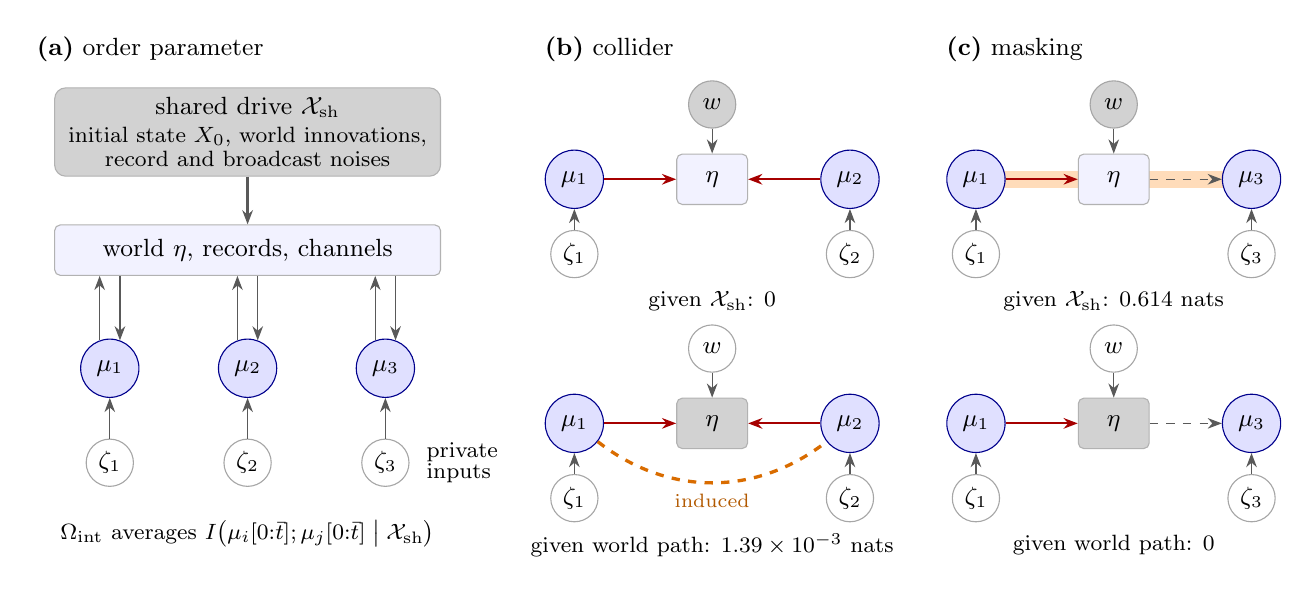
\begin{tikzpicture}[>={Stealth[length=1.8mm]}, every node/.style={font=\small},
    agent/.style={circle, draw=blue!55!black, fill=blue!12, inner sep=0pt, minimum size=7.4mm},
    priv/.style={circle, draw=gray!70, fill=white, inner sep=0pt, minimum size=6mm},
    drive/.style={circle, draw=gray!70, fill=white, inner sep=0pt, minimum size=6mm},
    world/.style={rectangle, rounded corners=2pt, draw=gray!60, fill=blue!5, inner sep=0pt, minimum width=9mm, minimum height=6.4mm},
    cond/.style={fill=gray!35},
    act/.style={->, thick, red!65!black},
    sense/.style={->, gray!70!black, dashed},
    inp/.style={->, gray!70!black},
    dep/.style={orange!85!black, very thick, dashed},
    hl/.style={line width=6pt, orange!60, opacity=0.45, line cap=round}]
  % panel (a): the conditioning set of the order parameter
  \node[anchor=west] at (-0.1,3.2) {\textbf{(a)} order parameter};
  \node[draw=gray!60, cond, rounded corners=4pt, minimum width=4.9cm, minimum height=1.05cm, align=center] (sh) at (2.7,2.15)
    {shared drive $\mathcal X_{\mathrm{sh}}$\\[-1pt]{\footnotesize initial state $X_0$, world innovations,}\\[-2pt]{\footnotesize record and broadcast noises}};
  \node[world, minimum width=4.9cm, minimum height=6.4mm] (ext) at (2.7,0.65) {world $\eta$, records, channels};
  \draw[inp, thick] (sh) -- (ext);
  \foreach \k/\x in {1/0.95, 2/2.7, 3/4.45} {
    \node[agent] (ma\k) at (\x,-0.85) {$\mu_{\k}$};
    \node[priv] (za\k) at (\x,-2.05) {$\zeta_{\k}$};
    \draw[inp] (za\k) -- (ma\k);
    \draw[->, gray!70!black] (ma\k.110) -- (ext.south -| ma\k.110);
    \draw[->, gray!70!black] (ext.south -| ma\k.70) -- (ma\k.70);
  }
  \node[anchor=west, font=\footnotesize, align=left] at (4.85,-2.05) {private\\[-2pt]inputs};
  \node[font=\footnotesize, align=center] at (2.7,-2.95) {$\Omega_{\mathrm{int}}$ averages $I\bigl(\mu_i[0{:}\bar t];\mu_j[0{:}\bar t]\bigm|\mathcal X_{\mathrm{sh}}\bigr)$};
  % panels (b) and (c): two readings of one model
  % each panel shows one model twice: conditioned on the shared drive (top) and on the world path (bottom)
  \node[anchor=west] at (6.35,3.2) {\textbf{(b)} collider};
  \node[anchor=west] at (11.45,3.2) {\textbf{(c)} masking};
  % (b) collider, given the shared drive
  \begin{scope}[shift={(6.85,1.55)}]
    \node[agent] (b1) at (0,0) {$\mu_1$};
    \node[world] (be) at (1.75,0) {$\eta$};
    \node[agent] (b2) at (3.5,0) {$\mu_2$};
    \node[drive, cond] (bw) at (1.75,0.95) {$w$};
    \node[priv] (bz1) at (0,-0.95) {$\zeta_1$};
    \node[priv] (bz2) at (3.5,-0.95) {$\zeta_2$};
    \draw[inp] (bw) -- (be);
    \draw[inp] (bz1) -- (b1);
    \draw[inp] (bz2) -- (b2);
    \draw[act] (b1) -- (be);
    \draw[act] (b2) -- (be);
    \node[font=\footnotesize] at (1.75,-1.55) {given $\mathcal X_{\mathrm{sh}}$: $0$};
  \end{scope}
  % (b) collider, given the world path
  \begin{scope}[shift={(6.85,-1.55)}]
    \node[agent] (b1) at (0,0) {$\mu_1$};
    \node[world, cond] (be) at (1.75,0) {$\eta$};
    \node[agent] (b2) at (3.5,0) {$\mu_2$};
    \node[drive] (bw) at (1.75,0.95) {$w$};
    \node[priv] (bz1) at (0,-0.95) {$\zeta_1$};
    \node[priv] (bz2) at (3.5,-0.95) {$\zeta_2$};
    \draw[inp] (bw) -- (be);
    \draw[inp] (bz1) -- (b1);
    \draw[inp] (bz2) -- (b2);
    \draw[act] (b1) -- (be);
    \draw[act] (b2) -- (be);
    \draw[dep] (b1) to[bend right=38] node[pos=0.5, below=0pt, font=\scriptsize, orange!70!black] {induced} (b2);
    \node[font=\footnotesize] at (1.75,-1.55) {given world path: $1.39\times10^{-3}$ nats};
  \end{scope}
  % (c) masking, given the shared drive
  \begin{scope}[shift={(11.95,1.55)}]
    \draw[hl] (0.37,0) -- (1.75,0) -- (3.13,0);
    \node[agent] (c1) at (0,0) {$\mu_1$};
    \node[world] (ce) at (1.75,0) {$\eta$};
    \node[agent] (c3) at (3.5,0) {$\mu_3$};
    \node[drive, cond] (cw) at (1.75,0.95) {$w$};
    \node[priv] (cz1) at (0,-0.95) {$\zeta_1$};
    \node[priv] (cz3) at (3.5,-0.95) {$\zeta_3$};
    \draw[inp] (cw) -- (ce);
    \draw[inp] (cz1) -- (c1);
    \draw[inp] (cz3) -- (c3);
    \draw[act] (c1) -- (ce);
    \draw[sense] (ce) -- (c3);
    \node[font=\footnotesize] at (1.75,-1.55) {given $\mathcal X_{\mathrm{sh}}$: $0.614$ nats};
  \end{scope}
  % (c) masking, given the world path
  \begin{scope}[shift={(11.95,-1.55)}]
    \node[agent] (c1) at (0,0) {$\mu_1$};
    \node[world, cond] (ce) at (1.75,0) {$\eta$};
    \node[agent] (c3) at (3.5,0) {$\mu_3$};
    \node[drive] (cw) at (1.75,0.95) {$w$};
    \node[priv] (cz1) at (0,-0.95) {$\zeta_1$};
    \node[priv] (cz3) at (3.5,-0.95) {$\zeta_3$};
    \draw[inp] (cw) -- (ce);
    \draw[inp] (cz1) -- (c1);
    \draw[inp] (cz3) -- (c3);
    \draw[act] (c1) -- (ce);
    \draw[sense] (ce) -- (c3);
    \node[font=\footnotesize] at (1.75,-1.55) {given world path: $0$};
  \end{scope}
\end{tikzpicture}

  \caption{\textbf{What the interaction order parameter conditions on.} Gray nodes are conditioned on. (a) The joint process is a function of the shared exogenous drive $\mathcal X_{\mathrm{sh}}$, which enters through the external states, and of each agent's private inputs $\zeta_i$: sensing noise, receiver-specific channel and read noise, and internal and policy randomness. The order parameter $\Omega_{\mathrm{int}}$ of \cref{def:agy-order-parameter} averages over pairs of members the conditional mutual information of their paths given $\mathcal X_{\mathrm{sh}}$. (b) Two agents with private noise act on the world (red arrows) and neither sense it nor exchange messages (\cref{ex:agy-collider}). Given the shared drive, here the world innovations $w$ with the initial state, their paths are independent (zero to $1.8\times10^{-15}$); given the world path $\eta$ with the initial state they are dependent, $1.39\times10^{-3}$ nats over six rounds, because the world is a common effect of both agents' private noises. (c) Agent 1 acts on the world and agent 3 only senses it (dashed arrow), as in \cref{ex:agy-masking}. Given the shared drive the path through the world carries a real interaction, $0.614$ nats over six rounds; given the world path that path is blocked and the statistic is zero to $4\times10^{-16}$, as \cref{prop:agy-nulls-vanish}(b) requires. Orange marks the dependence that each reading detects.}
  \label{fig:agy-conditioning}
\end{figure}
% src: figure supplied with the section; numbers of ex:agy-collider, ex:agy-masking and chk:agy-nulls

\Cref{fig:agy-conditioning} shows the conditioning set of \eqref{eq:agy-omega} and the two ways in which conditioning on an agent-driven world path misreports interaction. Conditioning on the world path, which is correct when the world is exogenous, both hides interaction through acts and creates dependence between agents that never interact once agents drive the world; conditioning on the shared exogenous drive is correct in both cases. The order parameter is then compared with one family of nulls, each declared as one the structure must differ from, one it must survive, an explanation that limits the attribution, or a diagnostic.

\begin{definition}[The null family]\label{def:agy-nulls}
A null is an intervention on the full model that keeps the world's dynamics, the agents' sensing of $\eta$, their priors, preferences and habits, unless it says otherwise; each deletion is specified per channel type (direct messages, record reads and traces of acts). The nulls and their types are those of \cref{tab:agy-nulls}. A structure differs from a null of type D when, on a nonempty open subset of the admitted class and for each constant of the selector, the selected partition differs from the null's, which is clause (F5) of the author's formation standard \citep{dennis2026formation}. Under the random null $\mathfrak N_{\mathrm{pr}}$ the selected partition is a random variable, and the structure differs from it when the test of \cref{prop:agy-tests}(b), applied to the statistic of the declared selector, rejects at a declared level $\alpha_{\mathrm{pr}}$ with a declared number $n_{\mathrm{null}}$ of null draws. A null whose intervention leaves the model unchanged is not applicable, is reported as such and imposes no requirement: $\mathfrak N_{\mathrm{hab}}$ in a model without policy selection by expected free energy, as under fixed or exogenously scheduled attention, and $\mathfrak N_{\mathrm{eff}}$ and $\mathfrak N_{\mathrm{inf}}$ in a model without acts. A structure survives a null of type S when the same partition is selected under the null with its blocks at contrast $r\ge r_0$; agreement with a null of type E is reported and restricts the claim; diagnostics are reported beside the verdict.
\end{definition}
% src: B4-D4 (merges L2-D13, L7-D4 and the earlier report's nulls)

\begin{table}[tbp]
\centering
\small
\setlength{\tabcolsep}{4pt}
\begin{tabular}{@{}>{\raggedright\arraybackslash}p{1.25cm}>{\raggedright\arraybackslash}p{4.5cm}>{\raggedright\arraybackslash}p{3.3cm}>{\raggedright\arraybackslash}p{2.7cm}>{\raggedright\arraybackslash}p{3.6cm}@{}}
\toprule
Null & Operation & Removes & Type & Order parameter and contrast \\
\midrule
$\mathfrak N_{\mathrm{lp}}$ & each inter-agent channel delivers pure noise; slots, capacities and assigned precisions kept & all informational coupling; keeps the attention pattern & D (weak) & $\Omega_{\mathrm{int}}=0$ when acts are also decoupled, and then $r\le1$ without records \\
$\mathfrak N_{\mathrm{rn}}$ & as $\mathfrak N_{\mathrm{lp}}$, with the deleted capacity reassigned to the remaining sources & the same, with reallocated attention & D (weak), same verdict as $\mathfrak N_{\mathrm{lp}}$ & as above \\
$\mathfrak N_{\mathrm{fr}}$ & every other agent held at its initial state in every term of an agent's update and action law & feedback through other agents & D (weak) & $\Omega_{\mathrm{int}}=0$ with broadcast noise in $\mathcal X_{\mathrm{sh}}$ when acts are also decoupled, and then $r\le1$ given $\mathcal X_{\mathrm{sh}}$ \\
$\mathfrak N_{\mathrm{eff}}$ & each act's effect on $\eta$ replaced by exogenous forcing with the law of the act path, added to $\mathcal X_{\mathrm{sh}}$ & physical feedback through the world & D for collectives said to form by joint action; makes the three nulls above separating & $\Omega_{\mathrm{int}}=0$ together with them \\
$\mathfrak N_{\mathrm{inf}}$ & acts keep their effect on $\eta$; every channel through which others read the act itself delivers noise & the informational trace of acts & D for collectives said to form by communication through acts & $\Omega_{\mathrm{int}}>0$ generically \\
$\mathfrak N_{\mathrm{pr}}$ & each receiver's partners redrawn uniformly at its attention rate and participation ratio, once or every round & who hears whom; keeps the volume & D (decisive) & $\Omega_{\mathrm{int}}>0$ generically; compare the selector \\
$\mathfrak N_{\mathrm{hab}}$ & $\gamma=0$: policies drawn from habits & selection by expected free energy & D & \\
$\mathfrak N_{\mathrm{ex}}$ & every receiver's literal likelihood, fusion and attention replaced by exact fusion, with provenance for records & misreading of joint structure & S (persistence) & same partition, blocks at $r\ge r_0$ \\
$\mathfrak N_{\mathrm w}$ & structure predicted from world dynamics and sensing access alone & attribution to access & E & partition distance \\
$\mathfrak N_{\mathrm{code}}$ & structure predicted from effective codes alone & attribution to code geometry & E & partition distance \\
$\mathfrak N_{\mathrm{fg}}$ & forgetting switched off & dependence on forgetting & diagnostic & reported \\
\bottomrule
\end{tabular}
\caption{The null family of \cref{def:agy-nulls}. D: the selected structure must differ from the null; S: it must survive the null; E: an explanation null, whose agreement with the structure is reported and limits the attribution.}
\label{tab:agy-nulls}
\end{table}

The declared types have reasons, given in full in the Supplement (\cref{sup:agy-interaction-order-parameter-and-tests}). The deletion and freezing nulls are weak, because any communication at all differs from them, and they certify interaction in the population and not among the members of a candidate $C$. Partner randomization at matched rates keeps the amount of communication and destroys its arrangement, which makes it the decisive differ null. The exact-fusion null removes only a misspecification, so a structure that vanishes under it is attributed to misreading of joint structure (\cref{sec:mis}), and the explanation nulls restrict the claim without removing interaction.

\begin{proposition}[Operational tests]\label{prop:agy-tests}
\begin{enumerate}
\item[(a)] (Interaction.) From $n_{\mathrm{rep}}$ independent replicate windows in which the shared drive is recorded, let $U_i$ and $U_j$ be the coordinates of the paths $\mu_i[0{:}\bar t]$ and $\mu_j[0{:}\bar t]$ that are not measurable with respect to $\mathcal X_{\mathrm{sh}}$, which excludes the initial states $\mu_i(0)$ and $\mu_j(0)$ because $X_0$ belongs to the shared drive, and assume that $\Cov((U_i,U_j)\mid\mathcal X_{\mathrm{sh}})$ is nonsingular and $n_{\mathrm{rep}}>\dim\mathcal X_{\mathrm{sh}}+\dim U_i+\dim U_j+1$. Let $\hat I$ be the plug-in conditional mutual information of $U_i$ and $U_j$ given $\mathcal X_{\mathrm{sh}}$, computed from the maximum-likelihood Gaussian covariance; its population value is the pair's term in \eqref{eq:agy-omega}, since the omitted coordinates are functions of the conditioning set. Then $2n_{\mathrm{rep}}\hat I$ is the Gaussian likelihood-ratio statistic for $\Cov(U_i,U_j\mid\mathcal X_{\mathrm{sh}})=0$, and under a causally separating null, as $n_{\mathrm{rep}}\to\infty$ with the dimensions fixed, it converges in law to the chi-squared law with $\dim U_i\cdot\dim U_j$ degrees of freedom.
\item[(b)] (Structure.) Let $\mathcal S_0$ be the value of the declared selector's statistic in the full model and $\mathcal S_1,\dots,\mathcal S_{n_{\mathrm{null}}}$ independent draws under $\mathfrak N_{\mathrm{pr}}$, and reject the null at level $\alpha$ when $p=(1+\#\{l:\mathcal S_l\ge\mathcal S_0\})/(n_{\mathrm{null}}+1)\le\alpha$. If $\mathcal S_0,\dots,\mathcal S_{n_{\mathrm{null}}}$ are exchangeable, which is the null hypothesis that the observed structure is a draw from the null model, then $\Pr(p\le\alpha)\le\alpha$.
\end{enumerate}
Proof in \cref{app:agy}; checked in \cref{chk:agy-tests}.
\end{proposition}
% src: B4-P6(a),(b)

Part (a) is Wilks's theorem \citep{wilks1938large} applied to the conditional cross-covariance block. At moderate sample sizes the test is liberal; a finite-sample multiplier whose support here is numerical, the selector used in part (b) when directed attention leaves contrast undefined, and a worked comparison with partner randomization are in the Supplement (\cref{sup:agy-interaction-order-parameter-and-tests}). Generic positivity of $\Omega_{\mathrm{int}}$ under attention selected by expected free energy, and an estimator of \eqref{eq:agy-omega} when the shared drive is not recorded, are open (\cref{open:agy-attention-positivity,open:agy-unrecorded-drive}).

\subsection{Hypothesis H1 in final form}\label{sec:agy-h1}

We can now say what a meta-agent is in this framework and which of H1's claims about it are theorems. The boundary property is not part of the definition, because every candidate with separate channels has it.

\begin{definition}[Meta-agent]\label{def:agy-meta-agent}
A set $C$ of agents is a meta-agent of grade $(r_0,\alpha_{\mathrm M},\alpha_{\mathrm I},\alpha_{\mathrm{pr}},\Agency_0)$ when it is a collective at the declared level $r_0$ (\cref{def:col-collective}); it is closed at tolerances $(\alpha_{\mathrm M},\alpha_{\mathrm I})$ for a declared coarse variable, with $\alpha_\Xi$ in place of $\alpha_{\mathrm M}$ when the declared memory measure is the Markov error (\cref{def:agy-closure}); it differs from every applicable null of type D, from $\mathfrak N_{\mathrm{pr}}$ at level $\alpha_{\mathrm{pr}}$ with the declared number $n_{\mathrm{null}}$ of null draws, and survives every null of type S in \cref{def:agy-nulls}, with the inapplicable nulls and its agreement with the nulls of type E reported; and its agency index on declared decision states is at least $\Agency_0$ (\cref{def:agy-agency-index}). The nulls of type D act on the whole population, so the differ clause concerns interaction in the population; that the members of $C$ interact with one another is the separate statement $\Omega_{\mathrm{int}}(C\mid\zeta_{V\setminus C})>0$ of \cref{def:agy-order-parameter}, reported with the grade.
\end{definition}
% src: F_brief H1 (graded meta-agenthood), B4-D5, B4-D4, L2-D11, B1-D3

\begin{theorem}[H1, final form]\label{thm:agy-h1}
Let $C$ be a set of agents of the linear-Gaussian framework with channel-level roles and per-channel noise, on a fixed or exogenously scheduled attention pattern, whose world-conditional law satisfies the moment bound.
\begin{enumerate}
\item[(a)] (Boundary, every $C$.) The canonical partition of $C$ is an exact path blanket from every conditionally independent start if, and generically only if, no sensory channel of $C$ reads an interior and an exterior variable in the same round: when one does, the path blanket fails outside a set of coefficients of positive codimension (\cref{thm:col-path-blanket}(b)). When the world-conditional covariance decays exponentially and is bounded with bounded inverse on a graph of polynomial growth, regions with finite interior whose shells are thick on the scale of an explicit bound on the Markov length are approximate stationary blankets of the world-conditional law, and the correlation length does not control the Markov length (\cref{thm:col-boundary}(b),(c)). The property holds for every candidate with separate channels and selects nothing (\cref{prop:col-selects-nothing}).
\item[(b)] (Contrast and the deletion nulls.) Let the members' world-conditional errors be scalar and the world-conditional precision diffusive. Under the deletion nulls of \cref{tab:agy-nulls}, combined with $\mathfrak N_{\mathrm{eff}}$ when members act, $\Omega_{\mathrm{int}}=0$, and in a population without records no region has contrast above one; hence, for such a population, on every set of parameters, open in a class with diffusive world-conditional precisions, on which $C$ is a collective at a declared level $r_0>1$, $C$ differs from these nulls in the sense of \cref{def:agy-nulls}. If the support of the couplings contains within the window a directed path from $\mu_j$ to $\mu_i$ for two members $i\ne j$, with $\mu_j$ loading on a private input of $j$ of positive variance, $\Omega_{\mathrm{int}}(C)>0$ for all couplings outside a closed null set.
\item[(c)] (Contrast gives closure of the collective average.) If in addition the members' world-conditional errors follow the reversible diffusion with drift $\Pi^c_{CC}$, with the exterior held fixed, and $r(C)>1$, then with $s=\sigma_C/\xout(C)$ the average $y=\phi_C^\top x$ satisfies
\begin{equation}\label{eq:agy-h1-closure}
\Xi\le\frac{s^2}{r(C)(r(C)-1)^2},
\end{equation}
so the memory clause of \cref{def:agy-closure} holds for it at every tolerance $\alpha_\Xi$ above this value. For non-reversible drift $M$ the bound \eqref{eq:agy-markov-gen} holds with the drift-based contrast and the row and column dispersions (\cref{thm:agy-closure-average}(b)), and the drift-based rates differ from the corresponding Rayleigh quotients of the stationary precision by at most $\Vert J\Vert\Vert\Pi\Vert$ (\cref{prop:agy-drift-precision}).
\item[(d)] (Inferential closure depends on the interpretation level.) Under consensus on information contributions the members' beliefs approach the union-model posterior at the rate $\rho_\perp^{n_{\mathrm c}}$ in the number $n_{\mathrm c}$ of rounds of the consensus matrix (\cref{prop:agy-consensus}); under literal consensus at level 1 their believed precisions diverge, and their means converge to the union-model mean only when the prior is flat and the graph regular (\cref{prop:agy-literal-consensus}).
\item[(e)] (Agency depends on the protocol and on the members' beliefs, not on contrast.) Under (P1) to (P4) the deliberation chain is reversible exactly when the members agree on the redundancy of their inputs; its stationary law is then a group posterior when some belief has the agreed redundancies, in particular when the members' beliefs are translates of one law (\cref{thm:agy-agency}), and in every case it lies within the distances of \cref{thm:agy-heterogeneous} of the group posterior of any declared belief; joint performative acts obey \cref{thm:agy-joint-acts}. Without data sharing, a collective at any contrast level fails agency, for group models with product habits, slot-product preferences and $\gamma_C>0$, whenever its members' slots carry redundant information (\cref{ex:agy-no-data-sharing}).
\end{enumerate}
Proof in \cref{app:agy}.
\end{theorem}
% src: B1-T4, B4-P5, L2-T5, B3-T3, B3-R3, B4-P7, B4-P8, L2-T6, B4-L2, B4-P1, B4-T1, B4-T2, L2-X2

Parts (a), (b) and (d) of \cref{thm:agy-h1} are theorems in the linear-Gaussian framework with fixed or exogenously scheduled couplings, (c) is a theorem for continuous-time linear dynamics with the exterior held fixed, and (e) for finite policy sets under the deliberation protocol. What makes $C$ a meta-agent, the grade of \cref{def:agy-meta-agent} with the declared types of \cref{tab:agy-nulls}, is a definition, and no population analyzed here is shown to meet every clause of it. The full account of what is proved, computed and open, including the standing of the two-group formation model against \cref{def:agy-meta-agent}, is in the Supplement (\cref{rem:agy-h1-status}).

Whether some linear-Gaussian population and some set $C$ of its agents meet every clause of \cref{def:agy-meta-agent} at a stated grade with $r_0>1$ and $\Agency_0>0$, or the clauses are jointly unsatisfiable in a stated class of populations, is open (Supplement, \cref{open:agy-meta-agent-exists}, followed there by a prose reading of H1 in final form).

\Cref{lem:met-unit-coordinate}(b) gives the bound of \cref{thm:agy-h1}(c) for any unit coordinate in place of $\phi_C$, with the rates of the pair $(M,\phi)$. \Cref{thm:met-h5a} gives a meta-agent, under stated conditions, the structure of an agent at its own scale; contrast enters none of these properties, so they describe a meta-agent and select none, and selection stays with contrast above the baseline and with the null family (\cref{rem:met-no-selection}).

\section{Coherence}\label{sec:coh}
% src: F_brief H3 and A11; L3 Sections 0-3, 5, 6 (formation results excluded); L1-P29, L1-X6; L4-P17, L4-P19; L6-P7, L6-C1, L6-C2; L7-P8 to L7-P10, L7-G4, L7-G5, L7-G7, L7-G10; C_critic V7, V8, C4, C5, C8, C9; B5 Sections 3 and 5; C2_check Section 4.2 item 3 and S5; decisions 9, 12, 16, 18

Hypothesis H3 holds that the coherence of message passing is part of the mechanism by which collectives form. To make the claim testable we split coherence into three components, each a property of the edges or cycles of the attention graph. Fidelity is the information about external states that a message carries; calibration is the agreement between the precision a receiver assigns to a message and the message's actual reliability; consistency is the composition of the translations that receivers apply around cycles. None of them is a virtue by itself. A closed group can pass its messages faithfully, find them calibrated by its own agreement and translate them consistently while all its members share a large error about the world, which makes it an echo chamber (\cref{def:mis-echo}). Every coherence statement below is therefore paired with a statement about accuracy.

After the components (\cref{sec:coh-components}) we take calibration (\cref{sec:coh-calibration}) and consistency (\cref{sec:coh-consistency}) in turn, fidelity being treated in the Supplement (\cref{sec:coh-fidelity}), then failures that coherence statistics do not reveal: amplification of belief messages around cycles (\cref{sec:coh-amplification}), domains of incompatible codes (\cref{sec:coh-codes}) and the grounding tension (\cref{sec:coh-tension}); what this contributes to formation is summarized in the Supplement (\cref{sec:coh-formation}). The setting is the linear-Gaussian framework of \cref{sec:fw}: the world $\eta_{t+1}=F\eta_t+w_t$; recognition densities $q_i=\Ncal(m_i,P_i)$ stored as $\mu_i=U_im_i$; messages $T_cU_jm_j+\nu$, read through a code model $\hat H_{ij}$ of the effective code $H_j=T_cU_j$ or through a learned translation $\Theta_{ij}$ of $j$'s internal coordinates, whose true value is $U_iU_j^{-1}$ and whose mistranslation is $\Upsilon_{ij}$ (\cref{def:fw-translation}); the interpretation levels and calibration classes $\mathsf{C0}$, $\mathsf{C1g}$, $\mathsf{C1i}$, $\mathsf{C2}$ of \cref{def:fw-levels,def:fw-calibration}; and the level-0 network of \cref{def:fw-level0}, whose error splits into a common mode and a connected part (\cref{lem:fw-common-mode}). Correlation lengths refer to the connected part, the world-conditional law of \cref{def:col-world-conditional}, and statements about lengths carry the hypothesis labels of \cref{asm:sca-standing}.

\subsection{Three components of coherence, scored with accuracy}\label{sec:coh-components}

We fix a receiver $i$, a sender $j$ that $i$ attends and a round $t$, write $\mathcal I_i$ for the information $i$ holds before the message, its sensory history and the messages already received, and write $\mathcal G_{\mathrm a}=(V,\mathcal E_{\mathrm a})$ for the attention graph, with an edge $j\to i$ when $i$ attends $j$.

\begin{definition}[Components of coherence]\label{def:coh-components}
\begin{enumerate}\renewcommand{\labelenumi}{(\alph{enumi})}
\item Fidelity. The marginal fidelity of the message $y_{ij}$ is $I(\eta_t;y_{ij})$, its receiver fidelity is $I(\eta_t;y_{ij}\mid\mathcal I_i)$, and its believed fidelity is the mutual information between $\eta_t$ and $y_{ij}$ under $i$'s own generative model; at level 0, with code model $\hat H_{ij}$, assigned noise $\hat R_{ij}$ and claimed covariance $\hat P_i$, it is $\frac12\ln\det(I+\hat R_{ij}^{-1}\hat H_{ij}\hat P_i\hat H_{ij}^\top)$. Path versions replace $\eta_t$ by $\eta_{1:t}$.
\item Calibration. Write the messages that $i$ attends as $y_{ij}=\hat H_{ij}\eta_t+\tilde\nu_{ij}$, stack their errors into $\tilde\nu_i$, and let $i$ assign $\tilde\nu_i$ a covariance $\hat R_i$ and a cross-covariance with its prior error $e_i$; at level 0, $\hat R_i$ is block diagonal and the cross-covariance is zero. The assigned precision is marginally calibrated if $\hat R_{ij}=\Cov(\tilde\nu_{ij})$ for every attended $j$; the receiver is calibrated including correlations if $\hat R_i=\Cov(\tilde\nu_i)$ and its assigned cross-covariance is $\Cov(\tilde\nu_i,e_i)$; it is overconfident (underconfident) if its claimed posterior covariance lies below (above) its actual posterior mean-square-error matrix in the Loewner order.
\item Consistency. Let each edge $j\to i$ carry a translation $\Theta_{ij}\in\GL(K)$. A closed walk $\mathfrak c$ is a sequence of agents $i_0,i_1,\dots,i_L=i_0$ with an edge joining $i_{u-1}$ and $i_u$ for every step $u$, and its holonomy $\Hol(\mathfrak c)=\Theta^{(L)}\cdots\Theta^{(1)}$ composes $\Theta^{(u)}=\Theta_{i_ui_{u-1}}$ when step $u$ runs along its edge and $\Theta^{(u)}=\Theta_{i_{u-1}i_u}^{-1}$ when it runs against it. A configuration $\mu=(\mu_i)_{i\in V}$ is in consensus if $\mu_i=\Theta_{ij}\mu_j$ on every edge; these configurations form the consensus space $\mathrm{Cons}(\Theta)$. The translations are consistent on content $v$ at $i_0$ if every holonomy of a closed walk at $i_0$ fixes $v$, and flat if every such holonomy is the identity.
\item Scoring with accuracy. A coherence score of a set $C$ of agents is a pair: a quantity from (a) to (c), aggregated over the edges or cycles inside $C$, and the inaccuracy $\mathcal A_C=\min_{i\in C}\E\Vert m_i-\eta_t\Vert^2_{P_0^{-1}}$ of \cref{def:mis-echo}.
\end{enumerate}
\end{definition}
% src: L3-D1, L3-D2, L3-D4, F_brief H3, critic D5

Receiver fidelity is what an exact receiver extracts from a message and believed fidelity what the receiver thinks it extracts; the gap is the over- or undervaluation of \cref{sec:mis}. The pairing in (d) is forced by a symmetry: an error shared by all agents leaves every statistic of social innovations unchanged (\cref{lem:mis-social-blind}), so only sensory innovations, that is grounding, can certify accuracy. Receiver-side quantities have closed forms for a message $y=H_jm+\nu$ that carries $j$'s posterior mean $m$ of $\eta\sim\Ncal(0,P_0)$, with posterior covariance $P$: then $y=H_j(P_0-P)P_0^{-1}\eta+\nu'$ with $\nu'$ independent of $\eta$ and $\Cov(\nu')=H_j(P-PP_0^{-1}P)H_j^\top+R_c$ (\cref{lem:coh-one-message} in \cref{app:coh-fidelity}, which also gives the fidelity in closed form; checked in \cref{chk:coh-sdpi}). An exactly specified receiver must therefore represent the attenuated code $H_j(P_0-P)P_0^{-1}$ and the sender's estimation noise, both of which the level-0 model omits.

Fidelity decides how far content can travel. Along a Markov chain of jointly Gaussian relays the information about a source is multiplied at each hop by at most the squared top canonical correlation of that hop, and on the infinite ring of scalar level-0 agents the information that an agent's mean carries about the noise injected at a distant agent decays exponentially in their distance at twice the mass, the rate at which influence itself decays, each under the hypotheses stated there (Supplement,\cref{sec:coh-fidelity,prop:coh-relay,prop:coh-info-decay}).

\subsection{Calibration and withdrawal}\label{sec:coh-calibration}

Calibration learned from agreement certifies mutual predictability, not accuracy; the echo chambers that result are treated in \cref{sec:mis} (\cref{thm:mis-echo-chambers,prop:mis-exact-no-echo}). Its second role bears on formation: it decides whether a receiver can register that a sender's messages are mistranslated, and therefore whether inconsistency can move attention. A static model makes every quantity explicit.

\begin{definition}[Static two-group model]\label{def:coh-calibration-model}
The world $\eta\sim\Ncal(0,\sigma_\eta^2I_K)$ is drawn afresh in every round. Agent $j$ senses $s_j=\eta+v_j$, $v_j\sim\Ncal(0,R^s_jI_K)$, and broadcasts its posterior mean $m_j=g_js_j$, $g_j=\sigma_\eta^2/(\sigma_\eta^2+R^s_j)$, in its internal coordinates through the public code $T_c=I_K$ with channel noise $\Ncal(0,R_cI_K)$. Frames $U_j$ and translations $\Theta_{ij}$ are orthogonal, and receiver $i$ carries each message into world coordinates as in \cref{def:fw-translation}, receiving $\tilde y_{ij}=\Upsilon_{ij}m_j+\nu_{ij}$ with the mistranslation $\Upsilon_{ij}=U_i^{-1}\Theta_{ij}U_j$ of \eqref{eq:fw-mistranslation}, which is $I$ exactly when the translation is true; the channel noise, carried into world coordinates by $U_i^{-1}\Theta_{ij}$, is again $\Ncal(0,R_cI_K)$ because $U_i$ and $\Theta_{ij}$ are orthogonal, and we write it $\nu_{ij}$. In the plane $\Upsilon_{ij}=\mathrm{Rot}(\phi_{ij})$, with $\phi_{ij}$ the angle of $\Theta_{ij}$ minus that of $U_iU_j^{-1}$, the translation error of \cref{def:frm-two-group}. Two groups $A$ and $B$ have exact translations within groups and arbitrary orthogonal $\Upsilon_{ij}$ across them. Every receiver senses, attends at most $\kappa$ senders and, at $\gamma=\infty$ and without attention costs, maximizes its believed information about $\eta$, the epistemic part of its expected free energy. Under $\mathsf{C0}$ the likelihood of $\tilde y_{ij}$ does not depend on $\Upsilon_{ij}$; under $\mathsf{C1g}$ and $\mathsf{C1i}$ receiver $i$ models $\tilde y_{ij}$ as $g_j\eta$ plus isotropic noise whose variance $\hat r_{ij}$ matches the second moment of $\tilde y_{ij}-g_j\eta$ on grounded rounds ($\mathsf{C1g}$) or of the innovation $\tilde y_{ij}-g_jg_is_i$ ($\mathsf{C1i}$); under $\mathsf{C2}$ it knows $\Upsilon_{ij}$.
\end{definition}
% src: L3-D7, L3-D8, critic D5 (ladder mapping)

\begin{proposition}[$\mathsf{C0}$ receivers cannot withdraw]\label{prop:coh-c0-blind}
\begin{enumerate}\renewcommand{\labelenumi}{(\alph{enumi})}
\item For a $\mathsf{C0}$ receiver the expected free energy of an attention policy depends on the actual mistranslations only through the receiver's current belief, never through a term for the mistranslation itself.
\item In the static two-group model the believed information of a $\mathsf{C0}$ receiver depends only on claimed covariances, so its expected free energy and its policy posterior over attention sets do not depend on the $\Upsilon_{ij}$ at any policy precision; if its fixed assigned noise depends on a sender only through the sender's sensing noise, it is indifferent between in-group and cross-group senders with equal sensing noise.
\end{enumerate}
\end{proposition}
% src: L3-P14

Blindness has a price. With $\sigma_\eta^2=R^s_j=1$, $R_c=0.1$, $K=2$ and $\kappa=2$, a $\mathsf{C0}$ receiver that attends one in-group sender and one cross-group sender with $\Upsilon=\mathrm{Rot}(\pi)$ has mean-square error $0.708$ per coordinate, against $0.292$ with two in-group senders and $0.500$ from its own sensing alone (\cref{chk:coh-withdrawal}). A calibrated receiver registers mistranslation as noise and acts on it.
% src: L3-E7

\begin{theorem}[Withdrawal under calibration]\label{thm:coh-withdrawal}
In the static two-group model let receiver $i$ be of class $\mathsf{C1g}$ or $\mathsf{C1i}$.
\begin{enumerate}\renewcommand{\labelenumi}{(\alph{enumi})}
\item Its calibrated noise for sender $j$ is $\hat r_{ij}=R_c+g_j^2R^s_j+\hat r^{\mathrm{mt}}_{ij}$ with the mistranslation term $\hat r^{\mathrm{mt}}_{ij}=g_j^2\sigma_\eta^2\Vert\Upsilon_{ij}-I\Vert_F^2/K$ under $\mathsf{C1g}$ and $g_i$ times this under $\mathsf{C1i}$.
\item It attends the $\kappa$ senders with the largest calibrated precisions $\varpi_{ij}=g_j^2/\hat r_{ij}$, ties broken arbitrarily, or all senders if there are fewer than $\kappa$.
\item Let at least $\kappa$ in-group senders be available, with $\kappa$th largest in-group calibrated precision $\varpi^{\mathrm{in}}_{i(\kappa)}$. A cross-group edge $b\to i$ is withdrawn when
\begin{equation}\label{eq:coh-withdrawal}
\hat r^{\mathrm{mt}}_{ib}>\frac{g_b^2}{\varpi^{\mathrm{in}}_{i(\kappa)}}-R_c-g_b^2R^s_b,
\end{equation}
and if the reverse strict inequality holds for some cross-group sender, $i$ attends at least one cross-group sender. Ties aside, the attended graph splits along the cut between $A$ and $B$ if and only if every cross edge satisfies \eqref{eq:coh-withdrawal}. With homogeneous sensing noise every $\Upsilon_{ib}\ne I$ leads to withdrawal.
\end{enumerate}
\end{theorem}
% src: L3-T4; critic V7 (verdict holds, scope stated); attendance clause of (c) corrected: the reverse inequality guarantees some cross sender, not each

The left side of \eqref{eq:coh-withdrawal} is the cost of mistranslation in noise-equivalent units and the right side the information advantage of the cross-group sender. Under $\mathsf{C1i}$ mistranslation is detected only in proportion to the receiver's own sensing gain, so a receiver that does not sense is as blind as a $\mathsf{C0}$ receiver (\cref{lem:mis-social-blind}). The scope is narrow: a static world, infinite policy precision, orthogonal mistranslation, and a $\mathsf{C1}$ model that matches the variance of the mistranslated message but not its correlation with $\eta$. That misspecification is the mechanism. A receiver that knows $\Upsilon_{ij}$, as a $\mathsf{C2}$ receiver does, undoes it and pays no mistranslation cost. In this static model, where the errors of different messages and of the receiver's own sensing are independent given $\eta$, the calibrated model of the corrected message, $g_j\eta$ plus isotropic noise of variance $R_c+g_j^2R^s_j$, is then the exact conditional law, so knowing the translations already gives exact fusion. Withdrawal from inconsistent edges is therefore a calibration-level effect of misreading joint structure; for the dynamic two-group model, where knowing the translation errors falls short of full exact fusion, see the Supplement (\cref{sec:coh-formation}). Bounded-confidence models postulate a withdrawal threshold, which is derived here; those models are discussed in the Supplement (\cref{sec:rel-opinion}). In the dynamic level-0 network the calibrated cost is set by the covariance of the sender's belief with the world (\cref{lem:frm-calibration}). Proofs in \cref{app:coh-calibration}; checks in \cref{chk:coh-withdrawal}.

Withdrawal can fail when a cut separates complementary access to the world: in the instance computed there, a receiver that senses one coordinate keeps attending a mistranslated cross-group sender that senses both (Supplement, \cref{ex:coh-unique-information}).

When translations are learned from grounded rounds on attended edges, persistent inconsistency can sit only on edges attended finitely often (\cref{prop:frm-flattening}), and because attention feeds learning, split and merged configurations can both be stable (\cref{prop:frm-bistability}); these are the first links of the formation chain of \cref{sec:frm}.

\subsection{Consistency}\label{sec:coh-consistency}

Consistency asks whether the translations agents use compose to the identity around cycles; when they do not, no configuration of beliefs agrees on every edge, and the least disagreement that remains measures frustration. Receivers learn their translations of one another independently, so $\Theta_{ji}$ need not be $\Theta_{ij}^{-1}$, and the criterion must hold on directed graphs that are only weakly connected.

\begin{theorem}[Holonomy criterion; (a) is due to \citet{dennis2026magent}]\label{thm:coh-holonomy}
Let the edges of $\mathcal G_{\mathrm a}$ carry translations $\Theta_{ij}\in\GL(K)$ and fix a base agent $i_0$.
\begin{enumerate}\renewcommand{\labelenumi}{(\alph{enumi})}
\item If $\mathcal G_{\mathrm a}$ is strongly connected, $\mu\mapsto\mu_{i_0}$ is a linear bijection from $\mathrm{Cons}(\Theta)$ onto $\bigcap_{\mathfrak c}\mathrm{Fix}(\Hol(\mathfrak c))$, the intersection over the directed closed walks $\mathfrak c$ at $i_0$.
\item If $\mathcal G_{\mathrm a}$ is weakly connected and $\mathcal T$ is a spanning tree of its underlying undirected graph, $\mu\mapsto\mu_{i_0}$ is a linear bijection from $\mathrm{Cons}(\Theta)$ onto $\bigcap_{e\notin\mathcal T}\mathrm{Fix}(\Hol_e)$, where $\Hol_e$ is the holonomy of the closed walk that runs from $i_0$ through $\mathcal T$ to the tail of the non-tree edge $e$, crosses $e$ and returns through $\mathcal T$.
\item Consensus with content $v$ at $i_0$ exists if and only if every $\Hol_e$ fixes $v$, and on strongly connected graphs if and only if every directed closed-walk holonomy at $i_0$ fixes $v$. Full consensus, $\dim\mathrm{Cons}(\Theta)=K$, holds if and only if $\Theta_{ij}=g_ig_j^{-1}$ for some $g_i\in\GL(K)$.
\end{enumerate}
\end{theorem}
% src: L3-T3 (part 1 imported from MAgent Theory 2.0 ch. 17, part 2 new), L6-P7(a,b), L7-G4, critic C8

Partial consensus survives on the common fixed space of the holonomies. When every vector must be fixed, (b) is the balance test of gain graphs on a fundamental system of cycles \citep{zaslavsky1989biased}, read in later restatements; with gains $\pm1$ it is the balance of signed graphs \citep{harary1953notion}, whose two-camp partition \citep{cartwright1956structural} is the simplest inconsistency cut. Part (a) needs return paths: on the acyclic digraph $0\to1$, $1\to2$, $0\to2$ it would claim a $K$-dimensional consensus space, while for generic translations $\mathrm{Cons}(\Theta)=0$, as (b) gives (\cref{chk:coh-holonomy}). Proof in \cref{app:coh-consistency}.

The true translations of agents that encode one world through invertible encodings are flat, so consensus about $\eta$ is always possible in principle, and positive least frustration (\cref{prop:coh-frustration}) arises only from learned translations that differ from the true ones or from agents that do not encode one common world invertibly (Supplement, \cref{prop:coh-flat-true}).

\begin{proposition}[Frustration]\label{prop:coh-frustration}
Give each edge $j\to i$ a precision $\varpi_{ij}>0$ and each agent a positive-definite metric $M_i$, and define the frustration $\mathfrak F(\mu)=\sum_{j\to i}\varpi_{ij}\Vert\mu_i-\Theta_{ij}\mu_j\Vert^2_{M_i}$.
\begin{enumerate}\renewcommand{\labelenumi}{(\alph{enumi})}
\item $\mathfrak F(\mu)=\mu^\top\mathcal L\mu$ with $\mathcal L=\mathcal B^\top\mathcal B\succeq0$, where the incidence operator $\mathcal B$ has, for the edge $j\to i$, the block $\varpi_{ij}^{1/2}M_i^{1/2}$ at $i$ and $-\varpi_{ij}^{1/2}M_i^{1/2}\Theta_{ij}$ at $j$. Its kernel is $\mathrm{Cons}(\Theta)$, and on a weakly connected attention graph $\lambda_{\min}(\mathcal L)$, the least frustration per unit of content, is positive if and only if the holonomies $\Hol_e$ of \cref{thm:coh-holonomy}(b) have no common nonzero fixed vector.
\item On a cycle of $N$ agents, each attending its predecessor, with unit precisions, $M_i=I$ and orthogonal translations whose holonomy has eigenvalues $e^{\mathrm i\theta_1},\dots,e^{\mathrm i\theta_K}$, the spectrum of $\mathcal L$ consists of the numbers $2-2\cos((2\pi u-\theta_r)/N)$, $u=0,\dots,N-1$, $r=1,\dots,K$. If $\phi\in[0,\pi]$ is the smallest modulus of an eigen-angle, $\lambda_{\min}(\mathcal L)=4\sin^2(\phi/(2N))\approx\phi^2/N^2$.
\item Let the translations be orthogonal, $M_i=I$, $\varpi_{ij}\ge\varpi_{\min}$, and $\mathcal T$, $\Hol_e$ as in \cref{thm:coh-holonomy}(b). For each agent $i$ let $\mathcal C_i$ be a nonempty finite family of simple cycles through $i$, with holonomies $\Hol^{(i)}(\mathfrak c)$ based at $i$ and lengths $|\mathfrak c|$, and put $\mathcal D_i=|\mathcal C_i|^{-1}\sum_{\mathfrak c\in\mathcal C_i}|\mathfrak c|^{-1}(I-\Hol^{(i)}(\mathfrak c))^\top(I-\Hol^{(i)}(\mathfrak c))$. Then
\[ \frac{\varpi_{\min}}{N}\min_i\lambda_{\min}(\mathcal D_i)\le\lambda_{\min}(\mathcal L)\le\frac1N\lambda_{\min}\Bigl(\sum_{e\notin\mathcal T}\varpi_e(I-\Hol_e)^\top(I-\Hol_e)\Bigr), \]
and on a single cycle the lower bound is within the factor $\pi^2/4$ of the exact value in (b).
\end{enumerate}
\end{proposition}
% src: L3-P9 (restating MAgent ch. 17 Corollary Frustration, extended to weakly connected graphs through L3-T3), L3-P10, L3-P11, L7-G5

A defect $\phi$ around $N$ agents is spread as $\phi/N$ per edge, so long cycles dilute frustration. With orthogonal translations, $M_i=I$ and $\Theta_{ji}=\Theta_{ij}^{-1}$ on undirected graphs, $\mathcal L$ is, up to normalization, the connection Laplacian of \citet{singer2012vector}, whose spectrum is tied to the frustration of synchronization by a Cheeger-type inequality (Supplement, \cref{sec:rel-sync}); we use none of its constants. Part (a) extends to weakly connected graphs a corollary of \citet{dennis2026magent}, and the lower bound in (c) can be loose by orders of magnitude (\cref{chk:coh-frustration}). Proofs in \cref{app:coh-consistency}.

With rank-limited codes only what is talked about must agree, and coded consensus is the space of global sections of a cellular sheaf, which the holonomy criterion does not characterize (Supplement, \cref{prop:coh-coded}). Under the hypotheses stated there, frustration raises the effective leak of agents that average transported content without sensing (\cref{prop:coh-frustration-grounding}), and cycles on which only edges of small mistranslation are attended have small least frustration whatever their length, although their holonomy can be large (\cref{prop:coh-attended-frustration}). Frustration bounds for translations in $\GL(K)$ are an open problem (\cref{open:coh-frustration-metric}).

\subsection{Amplification by mismatched prior structure}\label{sec:coh-amplification}

A receiver lifts a message into its full belief space and fills the directions the message does not carry from its own prior (\cref{prop:fw-prior-completion}). Composed around a cycle of receivers, these lifts can amplify content even when every code and every translation is correct, a failure that none of the three components registers.

\begin{definition}[Cycle product]\label{def:coh-cycle-product}
Let the $N$ agents of a population form a directed cycle $\mathfrak c$ in which agent $k+1$ receives from agent $k$, indices modulo $N$. Receiver $j$ has prior covariance $P_j\succ0$; sender $i$ has effective code $H_i$ and is read with assigned noise $\hat R_i\succeq0$, with $S_{ji}=H_iP_jH_i^\top+\hat R_i\succ0$. The edge map is the gain-code map $A_{ji}=\Kg_{ji}H_i$, $\Kg_{ji}=P_jH_i^\top S_{ji}^{-1}$, the linear response of the receiver's mean to the sender's mean at level 0; for noiseless codes it is the projector of \cref{prop:fw-prior-completion}(d). The cycle product is $A_{\mathfrak c}=A_{1N}A_{N,N-1}\cdots A_{21}$, and the cycle amplifies when $\rho(A_{\mathfrak c})>1$.
\end{definition}
% src: B5-D4, L4-P19(a), L1-P29(a)

The nonzero spectrum of $A_{\mathfrak c}$ does not depend on where the product starts, and frames enter only by conjugation, since in internal coordinates the edge map is $U_jA_{ji}U_i^{-1}$.

\begin{theorem}[Edge-ratio bound]\label{thm:coh-amplification}
\begin{enumerate}\renewcommand{\labelenumi}{(\alph{enumi})}
\item For an edge $e=(i\to j)$ put $X_{ji}=H_iP_jH_i^\top$, $X_{ii}=H_iP_iH_i^\top$, the edge ratio $\mathfrak r_e=\lambda_{\max}(S_{ji}^{-1}X_{ii})$, and $\mathrm{snr}_e$ through $\mathrm{snr}_e/(1+\mathrm{snr}_e)=\lambda_{\max}(S_{ji}^{-1}X_{ji})$, so that $\mathrm{snr}_e=\lambda_{\max}(\hat R_i^{-1/2}X_{ji}\hat R_i^{-1/2})$ when $\hat R_i\succ0$ and $\mathrm{snr}_e=\infty$ for noiseless codes. Then
\begin{equation}\label{eq:coh-edge-ratio}
\rho(A_{\mathfrak c})\le\prod_{e\in\mathfrak c}\Bigl(\mathfrak r_e\frac{\mathrm{snr}_e}{1+\mathrm{snr}_e}\Bigr)^{1/2}\le\prod_{e\in\mathfrak c}\mathfrak r_e^{1/2},
\end{equation}
so a cycle can amplify only if $\mathfrak r_e>1$ on some edge.
\item If the codes are noiseless and have rank below $K$, a story that leaves agent $1$ returns after $n$ circulations through $\bar A_{\mathfrak c}^n$, with the round-trip map $\bar A_{\mathfrak c}=(I-A_{1N})+A_{\mathfrak c}$, and $\rho(\bar A_{\mathfrak c})=\max\{\rho(A_{\mathfrak c}),1\}$; the story grows geometrically if and only if the cycle amplifies.
\end{enumerate}
\end{theorem}
% src: B5-T2, B5-P16, L1-X6, L4-P19(b,c); decision 9

The edge ratio compares the sender's prior variance in the directions its code carries with the receiver's predictive variance of the message, including the noise the receiver assigns. A cycle can amplify only where the receiver's assigned precision does not account for the sender's own uncertainty, which is a failure of calibration. Proof in \cref{app:coh-amplification}; random cycles never violated either bound, and the sharper one was attained to four digits (\cref{chk:coh-amplification}).

Amplification is excluded by a common prior covariance, by a spread of priors that is small against the assigned noise, by assigned noise that covers the sender's coded uncertainty, and by a common code read with common positive-definite noise, each in the precise form stated there (Supplement, \cref{prop:coh-no-amplification}); explicit amplifying cycles, among them noiseless cycles, for which no spread condition suffices and which amplify at arbitrarily small spread of priors, are in \cref{ex:coh-amplification}.

Amplification does not need misspecified priors: it is a numerical observation that level-0 cycles with codes of rank one still amplify when every prior is the exact posterior of one common prior given private linear-Gaussian data (Supplement, \cref{obs:coh-amplification-information}). Its classification under calibration and the open case of noisy circulation are in \cref{rem:coh-amplification-class,open:coh-amplification-noisy}.

\subsection{Code domains and conformity}\label{sec:coh-codes}

Codes are conventions: which sign, orientation or word a public feature carries. A code is arbitrary in a way a belief about $\eta$ is not, so grounding cannot fix it; what fixes it is the value of being understood, against which stand each agent's idiosyncratic preferences. We derive conformity from expected free energy and bound the size of the domains in which one code holds.

\begin{definition}[Code game]\label{def:coh-code-game}
Agents on an attention graph whose edges are attended in both directions each choose a code $\sigma_i\in\{\pm1\}$ for a public feature, used both to send and to read. On an attended edge, matching codes give a true translation and mismatched codes the mistranslation $-I$ on the feature's coordinates. Receivers are $\mathsf{C1}$-calibrated (\cref{thm:coh-withdrawal}): receiver $i$ assigns isotropic precision $\varpi^{=}$ to a matched message and $\varpi^{\neq}<\varpi^{=}$ to a mismatched one, and holds precision $\Lambda^{\mathrm{own}}$ from its prior and its own sensing. If $i$ has $\mathsf d_i$ partners, $u_i(\sigma)$ of whom use code $\sigma$, its believed information with code $\sigma$ is $\mathcal F_i(u_i(\sigma))$, where
\begin{equation}\label{eq:coh-value}
\mathcal F_i(u)=\frac K2\ln\Bigl(1+\frac{u\varpi^{=}+(\mathsf d_i-u)\varpi^{\neq}}{\Lambda^{\mathrm{own}}}\Bigr),
\end{equation}
with $u$ replaced by $\min\{u,\kappa\}$ and $\mathsf d_i$ by $\kappa$ under a capacity $\kappa<\mathsf d_i$. Each agent also has a pull $h_i$, a prior preference for its native code that enters its expected free energy, so that $G_i(\sigma)=-\mathcal F_i(u_i(\sigma))-h_i\sigma$ up to terms free of $\sigma$.
\end{definition}
% src: L3-D9, B5 Section 3.1, B5-L1

The pull must sit in the expected free energy, not in the habit $E_i$: a habit enters the policy posterior as $\ln E_i$ beside $-\gamma G_i$ and vanishes relative to the couplings as $\gamma\to\infty$. A value affine in $u$ with a slope common to all agents, as in the weak-message limit $\varpi^{=}\ll\Lambda^{\mathrm{own}}$ of \eqref{eq:coh-value}, makes the game pairwise. Away from that limit the value is concave in $u$, and with several features the value an edge loses to mistranslation is concave and subadditive in the number of mismatched features (\cref{lem:coh-c1-value}, in \cref{app:coh-codes}).

No preference for conformity is assumed: with uniform habits the policy posterior gives a logistic adoption rule that is nondecreasing in the local frequency of a code, with an innovation floor at finite policy precision and, for a value affine in $u$ with slope $J$ and no pull, two stable fixed points when $\gamma J\mathsf d_i>2$ (Supplement, \cref{prop:coh-adoption}).

\begin{proposition}[The code game as a potential game]\label{prop:coh-code-potential}
\begin{enumerate}\renewcommand{\labelenumi}{(\alph{enumi})}
\item If $G_i(\sigma)=\sum_jJ_{ij}\mathbf 1[\sigma\ne\sigma_j]-h_i\sigma$ up to terms free of $\sigma$, with symmetric couplings $J_{ij}=J_{ji}\ge0$ on attended edges, then $\Phi_{\mathrm{code}}(\sigma)=\sum_{\{i,j\}}J_{ij}\mathbf 1[\sigma_i\ne\sigma_j]-\sum_ih_i\sigma_i$ is an exact potential, and asynchronous logit revision, in which a uniformly chosen agent resamples its code from $q_i(\sigma)\propto e^{-\gamma G_i(\sigma)}$, is reversible with stationary law proportional to $e^{-\gamma\Phi_{\mathrm{code}}}$, which concentrates on the minimizers of $\Phi_{\mathrm{code}}$ as $\gamma\to\infty$.
\item If every agent has exactly two partners and all agents have the same nondecreasing value $\mathcal F$, the code game is the game of (a) with $J_{ij}=J=\frac12(\mathcal F(2)-\mathcal F(0))$ on every edge.
\item Write $\nabla^{\pm}\mathcal F_i(u)=\mathcal F_i(u+1)-\mathcal F_i(u)+\mathcal F_i(\mathsf d_i-u)-\mathcal F_i(\mathsf d_i-1-u)$ for $u\in\{0,\dots,\mathsf d_i-1\}$. An exact potential exists only if every attended edge $\{i,j\}$ satisfies the following: if $i$ and $j$ have the same other partners, then $\nabla^{\pm}\mathcal F_i(u)=\nabla^{\pm}\mathcal F_j(u)$ for every $u$, and otherwise $\nabla^{\pm}\mathcal F_i$ and $\nabla^{\pm}\mathcal F_j$ do not depend on $u$ and take the same value. Affine values with a common slope satisfy this on every graph, and a common quadratic value on regular graphs, with explicit pairwise potentials. A common value satisfies it on every complete graph, where $\Phi(\sigma)=-\sum_{c=\pm1}\sum_{k=0}^{n_c(\sigma)-1}\mathcal F(k)-\sum_ih_i\sigma_i$, with $n_c(\sigma)$ the number of agents that use code $c$, is an exact potential. For the value \eqref{eq:coh-value}, without capacity and with capacity one, $\nabla^{\pm}\mathcal F_i$ depends on $u$ at every agent with three partners, so a connected attention graph that contains such an agent and is not the complete graph on four agents admits no exact potential, and neither does an open chain of at least three agents.
\end{enumerate}
\end{proposition}
% src: L3-P18, B5-P10 (scope corrected: the ends of an open chain have one partner; affine values need a common slope)

Part (a) is the log-linear learning of \citet{blume1993statistical}, which we know from secondary sources, and by the four-cycle criterion of \citet[Theorem~2.8]{monderer1996potential}, read in the restatement of \citet{arefizadeh2024characterizations}, the condition in (c) is also sufficient. On a ring of four agents with couplings $1$ and $0.3$ in the two directions the logit chain violates detailed balance (\cref{chk:coh-codes}), so asymmetric attention destroys the potential. The code game with a common value is thus an exact potential game on rings and on complete graphs, where it is a congestion game, and on open chains of at least three agents only in its pairwise form. Proof in \cref{app:coh-codes}. For continuous conventions with quadratic conformity to attended partners and to cavity-read group records, the game is again an exact potential game, whose Gibbs precision is diffusive and fixed by the attended couplings, the pulls and the readership, so linear conformity selects no partition that these do not already contain (\cref{prop:hie-conformity}).

\begin{theorem}[One-dimensional code domains]\label{thm:coh-domains-1d}
Let $N\ge3$ agents form a ring, each attending its two neighbors with $\mathsf{C1}$-calibrated reception, let all agents have the same nondecreasing value $\mathcal F$ with $J=\frac12(\mathcal F(2)-\mathcal F(0))>0$, and in (a) and (b) let the pulls $h_1,\dots,h_N$ be the first $N$ terms of a sequence of independent $\Ncal(0,h^2)$ variables, $h>0$.
\begin{enumerate}\renewcommand{\labelenumi}{(\alph{enumi})}
\item Asynchronous logit code dynamics at policy precision $\gamma$ is reversible with stationary law proportional to $e^{-\gamma\Phi_{\mathrm{code}}}$, which concentrates as $\gamma\to\infty$ on the almost surely unique minimizer $\sigma^\ast_N$ of $\Phi_{\mathrm{code}}$, the stochastically stable configuration.
\item The mean domain length $\bar\ell_N$ of $\sigma^\ast_N$, the number of agents divided by the number of maximal runs of one code, satisfies almost surely
\[ \frac12\Bigl(\frac Jh\Bigr)^2\le\liminf_{N\to\infty}\bar\ell_N\le\limsup_{N\to\infty}\bar\ell_N\le26\Bigl(\frac Jh\Bigr)^2+7. \]
\item Without pulls and at finite $\gamma$, two agents at distance $d$ use different codes with probability $\frac12\bigl(1-\frac{\tanh^d(\gamma J/2)+\tanh^{N-d}(\gamma J/2)}{1+\tanh^N(\gamma J/2)}\bigr)$, which tends to $\frac12(1-\tanh^d(\gamma J/2))$ as $N\to\infty$; neighbors then differ with probability $1/(1+e^{\gamma J})$.
\end{enumerate}
\end{theorem}
% src: B5-T1, L3-T5, L3-L3, L3-L4, L3-L5, L3-P18, B5-P10; stated on rings, the chain version holding for the pairwise game

For the $\mathsf{C1}$ value with both partners attended $J=\frac K4\ln\frac{\Lambda^{\mathrm{own}}+2\varpi^{=}}{\Lambda^{\mathrm{own}}+2\varpi^{\neq}}$, and with capacity one $J=\frac K4\ln\frac{\Lambda^{\mathrm{own}}+\varpi^{=}}{\Lambda^{\mathrm{own}}+\varpi^{\neq}}$. Code domains on a ring therefore have a mean length of order the square of the ratio of the believed value lost to mistranslation to the strength of idiosyncratic preference. The scope is binary codes, a common value, asynchronous revision, Gaussian pulls and the stochastically stable state, whose time to be reached is not bounded here; agent-specific values give only a weighted potential game. Part (b) holds for the minimizer of the pairwise potential on an open chain as well, but there (a) needs affine values with a common slope (\cref{prop:coh-code-potential}(c)), and whether code domains have contrast in the sense of \cref{def:col-collective} is open (\cref{open:abs-code-contrast}). \Cref{ex:hie-code-domains} answers this for the declared precision of a belief network on a ring whose attention is cut at the walls between domains, with an answer that depends on the declared geometry, and \cref{conj:hie-conformity-formation} states the formation question that remains: whether the code game with member-written code records and a pragmatic coordination value produces such collectives from a disordered start. The proof (\cref{app:coh-codes}) compares the walls of $\sigma^\ast_N$ with the switches of a greedy hysteresis of the field walk $X_i=h_1+\cdots+h_i$. The constants are not sharp: in exact minimizers on chains of up to $1.5\times10^6$ agents the mean domain length divided by $(J/h)^2$ fell from $4.71$ at $J/h=1$ to $1.06$ at $J/h=32$ (\cref{chk:coh-domains}), and we conjecture that domains and switches agree in number up to one (\cref{conj:coh-walls}), in line with the real-space renormalization of the random-field Ising chain by \citet{fisher2001nonequilibrium}, whose abstract we read. In higher dimension the rigorous results concern random-field models, and their transfer to the code game is conjectural.

Three conjectures carry these questions further (Supplement): in the pairwise game with weak random pulls no code spans a large population in two dimensions while one code does in three or more (\cref{conj:coh-imry-ma}); without pulls the pairwise game on $\Z^2$ coarsens with domain size growing as $t^{1/2}$ (\cref{conj:coh-coarsening}); and a mismatch cost concave in the number of mismatched features makes the walls of different features attract, so that isoglosses, the boundaries of single features, bundle (\cref{conj:coh-bundling}).

\subsection{The grounding tension}\label{sec:coh-tension}

\Cref{asm:int-a11} says that grounding caps the correlation length but makes the collective informative. On a ring of level-0 receivers the trade-off is exact. Each agent senses a scalar world with $0<F<1$ through noise of variance $R^s$ and attends its two neighbors through channels of noise variance $R_c$, assigning precision $\varpi_{\mathrm s}$ to its sensing and $\varpi_{\mathrm y}$ to each message. Its claimed quantities solve $\hat\Lambda^+=1/\hat P^-+\varpi_{\mathrm s}+2\varpi_{\mathrm y}$ and $\hat P^-=F^2/\hat\Lambda^++Q$, its gains are $k^s=\varpi_{\mathrm s}/\hat\Lambda^+$ and $k_{ij}=k^{\mathrm y}=\varpi_{\mathrm y}/\hat\Lambda^+$, and the error-transfer matrix has $W_{ii}=c=F(1-k^s-2k^{\mathrm y})$ and $W_{ij}=a=Fk^{\mathrm y}$ for neighbors, with row sums $\lambda=c+2a=F(1-k^s)=1-\varepsilon$ and local noise variance $q=F^2((k^s)^2R^s+2(k^{\mathrm y})^2R_c)$.

\begin{theorem}[Grounding tension]\label{thm:coh-grounding-tension}
\begin{enumerate}\renewcommand{\labelenumi}{(\alph{enumi})}
\item On the infinite ring with the gains above, \textup{(NN)} and \textup{(C$_r$)} hold with $\lambda=1-\varepsilon<1$, hence \textup{(M)}, and:
\begin{enumerate}\renewcommand{\labelenumii}{(\roman{enumii})}
\item $a/\varepsilon=F\varpi_{\mathrm y}/((1-F)\hat\Lambda^++F\varpi_{\mathrm s})$, and the correlation length of the world-conditional law is $\xi=1/\arccosh(1+\varepsilon/(2a))$ hops. As $F\to1$ at fixed assigned precisions $a/\varepsilon\to\varpi_{\mathrm y}/\varpi_{\mathrm s}$; as $\varpi_{\mathrm y}\to\infty$, $a/\varepsilon\to F/(2(1-F))$ and $\xi\to1/\arccosh(1/F)$, which bounds $\xi$ at every assigned precision.
\item The stationary mean-square error of every agent is
\begin{equation}\label{eq:coh-ring-mse}
\E e_i^2=\frac{Q}{\varepsilon(2-\varepsilon)}+\frac q2\Bigl[\frac{1}{\sqrt{\varepsilon(1-c+2a)}}+\frac{1}{\sqrt{(1+c)^2-4a^2}}\Bigr].
\end{equation}
\item Hence
\begin{equation}\label{eq:coh-tension-law}
\E e_i^2\ge\frac{Q}{\varepsilon(2-\varepsilon)}\ge\frac{Q\xi^2}{2a\cosh^2(1/(2\xi))},
\end{equation}
so that $\E e_i^2\ge(Q/2a)\xi^2(1+O(\xi^{-2}))\ge(Q/F)\xi^2(1+O(\xi^{-2}))$.
\item As $\varpi_{\mathrm y}\to\infty$, $k^s\to0$ and $\E e_i^2\to P_0+F^2R_c/(2\sqrt{1-F^2})>P_0$.
\end{enumerate}
\item In any scalar level-0 network with exact code models satisfying \textup{(Lin)}, \textup{(Loc)}, \textup{(B)} and \textup{(NN)}, with time-invariant $W$, homogeneous sensing gain $k$ and $\lambda=F(1-k)<1$, every agent's stationary mean-square error and the correlation length $\xi$ of the world-conditional law satisfy
\[ \E e_i^2\ge\frac{Q}{1-e^{-2/\xi}}\ge\frac{Q\xi}{2}. \]
\end{enumerate}
\end{theorem}
% src: L3-P19, L3-P20; critic V8 (closed form confirmed to six digits); R3 for the decay rate; 0<F<1, (Loc) and exact codes made explicit

\begin{figure}[t]
  \centering
  % Figure: grounding tension on the level-0 ring (F=0.99, Q=0.02, sensing noise 1, channel noise 0.1).
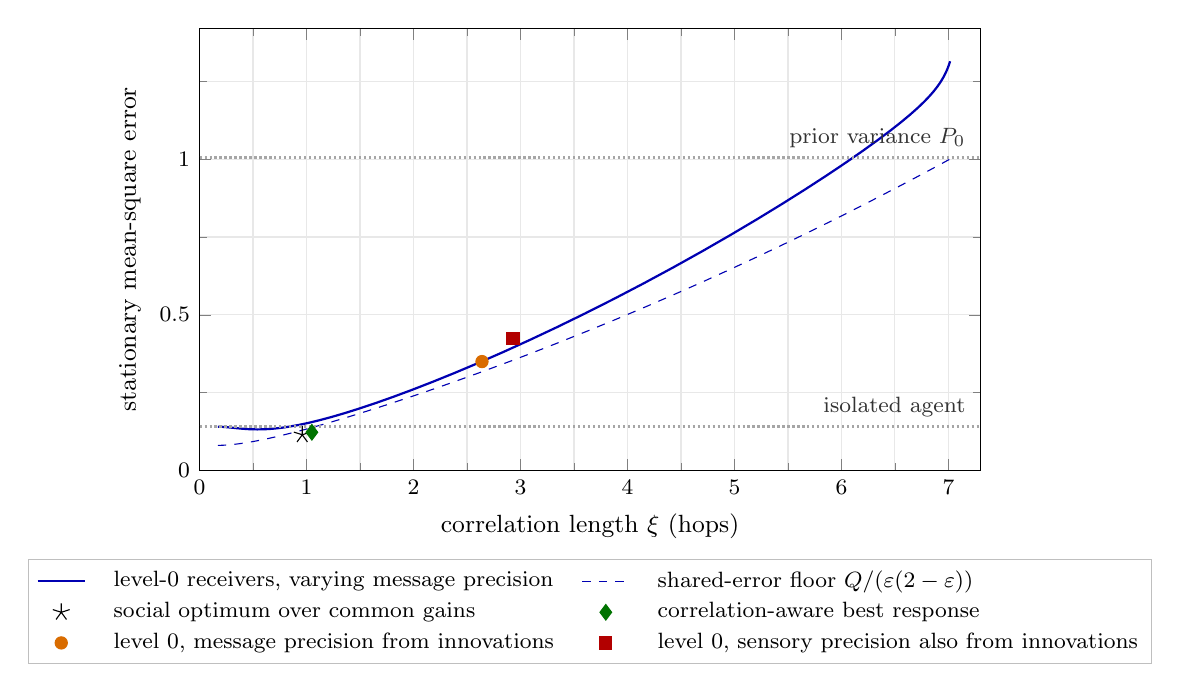
\begin{tikzpicture}
  \begin{axis}[width=11.5cm, height=7.2cm,
      xmin=0, xmax=7.3, ymin=0, ymax=1.42,
      xlabel={correlation length $\xi$ (hops)}, ylabel={stationary mean-square error},
      grid=both, grid style={gray!18}, minor tick num=1,
      legend style={font=\footnotesize, at={(0.5,-0.2)}, anchor=north, draw=gray!50, fill=white, cells={anchor=west}, legend columns=2, column sep=8pt},
      every axis label/.style={font=\small}, tick label style={font=\footnotesize}]
    \addplot[blue!70!black, thick] coordinates {(0.17121,0.14115) (0.17776,0.14107) (0.18483,0.14097) (0.19247,0.14086) (0.20074,0.14071) (0.20973,0.14054) (0.21952,0.14032) (0.23022,0.14006) (0.24194,0.13975) (0.25483,0.13937) (0.26904,0.13893) (0.28474,0.13841) (0.30216,0.13780) (0.32153,0.13712) (0.34312,0.13635) (0.36724,0.13553) (0.39425,0.13468) (0.42451,0.13385) (0.45848,0.13311) (0.49661,0.13256) (0.53941,0.13231) (0.58744,0.13252) (0.64127,0.13335) (0.70153,0.13498) (0.76886,0.13761) (0.84395,0.14143) (0.92749,0.14663) (1.02022,0.15340) (1.12287,0.16193) (1.23620,0.17238) (1.36095,0.18492) (1.49784,0.19973) (1.64754,0.21696) (1.81063,0.23679) (1.98760,0.25939) (2.17875,0.28492) (2.38415,0.31351) (2.60359,0.34528) (2.83650,0.38031) (3.08186,0.41858) (3.33819,0.46002) (3.60343,0.50444) (3.87501,0.55151) (4.14983,0.60077) (4.42437,0.65163) (4.69483,0.70337) (4.95734,0.75520) (5.20820,0.80627) (5.44414,0.85578) (5.66252,0.90301) (5.86148,0.94737) (6.04002,0.98846) (6.19794,1.02605) (6.33578,1.06010) (6.45467,1.09072) (6.55611,1.11813) (6.64184,1.14263) (6.71372,1.16456) (6.77355,1.18425) (6.82307,1.20203) (6.86385,1.21817) (6.89729,1.23292) (6.92463,1.24646) (6.94690,1.25892) (6.96501,1.27038) (6.97971,1.28090) (6.99162,1.29050) (7.00126,1.29919) (7.00905,1.30700) (7.01534,1.31394)};
    \addlegendentry{level-0 receivers, varying message precision}
    \addplot[blue!70!black, dashed] coordinates {(0.17121,0.08093) (0.17776,0.08099) (0.18483,0.08105) (0.19247,0.08113) (0.20074,0.08123) (0.20973,0.08136) (0.21952,0.08152) (0.23022,0.08171) (0.24194,0.08195) (0.25483,0.08224) (0.26904,0.08261) (0.28474,0.08306) (0.30216,0.08361) (0.32153,0.08430) (0.34312,0.08514) (0.36724,0.08618) (0.39425,0.08744) (0.42451,0.08898) (0.45848,0.09085) (0.49661,0.09312) (0.53941,0.09585) (0.58744,0.09912) (0.64127,0.10302) (0.70153,0.10764) (0.76886,0.11308) (0.84395,0.11945) (0.92749,0.12685) (1.02022,0.13541) (1.12287,0.14525) (1.23620,0.15650) (1.36095,0.16927) (1.49784,0.18372) (1.64754,0.19997) (1.81063,0.21816) (1.98760,0.23842) (2.17875,0.26088) (2.38415,0.28563) (2.60359,0.31276) (2.83650,0.34231) (3.08186,0.37425) (3.33819,0.40850) (3.60343,0.44488) (3.87501,0.48312) (4.14983,0.52284) (4.42437,0.56355) (4.69483,0.60467) (4.95734,0.64555) (5.20820,0.68551) (5.44414,0.72391) (5.66252,0.76016) (5.86148,0.79377) (6.04002,0.82442) (6.19794,0.85192) (6.33578,0.87622) (6.45467,0.89740) (6.55611,0.91564) (6.64184,0.93117) (6.71372,0.94428) (6.77355,0.95524) (6.82307,0.96436) (6.86385,0.97190) (6.89729,0.97810) (6.92463,0.98318) (6.94690,0.98732) (6.96501,0.99070) (6.97971,0.99344) (6.99162,0.99567) (7.00126,0.99747) (7.00905,0.99893) (7.01534,1.00011)};
    \addlegendentry{shared-error floor $Q/(\varepsilon(2-\varepsilon))$}
    \addplot[only marks, mark=star, mark size=3.2pt, black] coordinates {(0.96,0.115)};
    \addlegendentry{social optimum over common gains}
    \addplot[only marks, mark=diamond*, mark size=2.8pt, green!45!black] coordinates {(1.05,0.123)};
    \addlegendentry{correlation-aware best response}
    \addplot[only marks, mark=*, mark size=2.2pt, orange!85!black] coordinates {(2.64,0.350)};
    \addlegendentry{level 0, message precision from innovations}
    \addplot[only marks, mark=square*, mark size=2.2pt, red!70!black] coordinates {(2.93,0.425)};
    \addlegendentry{level 0, sensory precision also from innovations}
    \draw[gray!70, densely dotted, thick] (axis cs:0,1.005) -- (axis cs:7.3,1.005);
    \node[font=\footnotesize, gray!40!black, anchor=south east] at (axis cs:7.25,1.005) {prior variance $P_0$};
    \draw[gray!70, densely dotted, thick] (axis cs:0,0.1415) -- (axis cs:7.3,0.1415);
    \node[font=\footnotesize, gray!40!black, anchor=south east] at (axis cs:7.25,0.1415) {isolated agent};
  \end{axis}
\end{tikzpicture}

  \caption{\textbf{The grounding tension on the ring.} Stationary mean-square error of level-0 receivers on a ring against the correlation length $\xi$, as the precision assigned to messages varies ($F=0.99$, $Q=0.02$, sensing noise variance $1$, channel noise variance $0.1$). The dashed curve is the shared-error floor $Q/(\varepsilon(2-\varepsilon))$, which grows like $(Q/2a)\xi^2$. The marks show where agents settle: the social optimum over common gains and the correlation-aware best response sit near $\xi\approx1$, below the error of an isolated agent, while level-0 agents that calibrate message precision from social innovations sit far along the curve, and further still when they calibrate their senses the same way.}
  \label{fig:coh-tension}
\end{figure}

The first term of \eqref{eq:coh-ring-mse} is the shared error, which every agent carries and no agent can see in social innovations; the second is the connected part. On the grid of \cref{chk:coh-grounding} raising the precision on messages lengthens the correlation length, which is checked and not proved in general, while the shared-error floor grows at least quadratically in that length on the ring and at least linearly in any level-0 network with homogeneous grounding. Reach never exceeds its pure-listening limit $1/\arccosh(1/F)$, $7.04$ hops at $F=0.99$, and pure listening drives the error above the prior variance, a strong echo chamber in the sense of \cref{def:mis-echo}. An accuracy target therefore caps the correlation length: on the ring $\xi\lesssim\sqrt{2a\E e_i^2/Q}$. In \cref{fig:coh-tension} the error is smallest at a correlation length of $0.54$ hops, and the closed form agrees to six digits with a direct Lyapunov solution on a ring of 400 agents (\cref{chk:coh-grounding}). Proof in \cref{app:coh-tension}. A record that the members write from their own predictions carries the tension across levels: it slows the correction of an error they share with it (\cref{lem:hie-record-blind}) and raises the shared-error floor, which is nondecreasing in the weight the members give the record (\cref{thm:hie-floor}), and top-down precision assigned above its Kalman value trades disagreement for shared error (\cref{prop:hie-echo-tradeoff}).

Where agents settle on the curve is set by how they assign precision. A level-0 receiver that sets its message precision by minimizing free energy matches a moment that contains no shared error (Supplement, \cref{prop:coh-placement}), and in a numerical observation at the parameters of \cref{fig:coh-tension} such agents settle on the long-$\xi$, low-accuracy side of the social optimum (\cref{obs:coh-placement}); that the myopic equilibrium of correlation-aware agents senses less than the social optimum is conjectured (\cref{conj:coh-externality}).

Read together with the size bound of \cref{cor:col-lstar}, and only as an interpretation because the two bounds are proved in different settings, the tension suggests that large accurate collectives need more than homogeneous local message passing (Supplement, \cref{rem:coh-h4}).

What these results contribute to hypothesis H3, a qualified version in which calibrated receivers of the static two-group model withdraw attention from inconsistent edges under the condition of \cref{thm:coh-withdrawal} while a consistent and mutually calibrated interior can still be an echo chamber, is summarized with the status of the formation chain of \cref{sec:frm} in the Supplement (\cref{sec:coh-formation}).

\section{Formation}\label{sec:frm}
% src: B2 (whole note); L3-P15, L3-P16, L3-C1, L3-T4 as extended by B2-L1; L2-O3; L7-D4 and B4-D4; C2-4, C2-5; decisions 7, 11, 12

The preceding sections say what a collective is and how it is tested (\cref{sec:col,sec:agy}), but not that communicating agents arrive at one by themselves. This section takes up the formation half of hypothesis H3, the author's idea that coherent message passing is part of how meta-agents form: calibrated precision, scarce attention and grounded learning of translations should sort a population into collectives whose boundaries lie where translations are inconsistent. After stating what a formation result must show, we summarize two mechanisms, treated in the Supplement, and follow the chain in one model, two groups of agents whose private frames differ by a rotation.

The result is partial. In the two-group model at $\gamma=\infty$ with noiseless angle observations, clauses (T1) to (T3) and (T5) of \cref{def:frm-target} are theorems, the contrast clause (T3) at the levels of the window of \cref{thm:frm-split-contrast}(c), which is nonempty at every computed parameter point (Supplement, \cref{obs:frm-grid}); for $\gamma_S<\gamma<\infty$ reachability of the split branch is a theorem about the frozen-calibration mean-field map only; and clause (T4) fails for the translation-aware null of type S from a start law that is exchangeable given the world path, as the declared start with identical initial beliefs is, so from such a start the model yields no formation result in the sense of \cref{def:frm-target}. \Cref{sec:frm-status} gives the status clause by clause.

\subsection{What a formation result must show}\label{sec:frm-target}

A formation claim links a mechanism inside agents to a structure that a declared selector finds in their joint states, and it must exclude explanations that need no communication. We use the declared-selection clauses of the author's formation standard \citep{dennis2026formation} in the form of the null family of \cref{def:agy-nulls}.

\begin{definition}[Formation result]\label{def:frm-target}
Let a model of communicating agents have an open parameter set $\mathcal P$ in a Euclidean space and a declared start law, and let collectives be selected as in \cref{def:col-collective}, by contrast on the world-conditional precision at a level $r_0$ declared in advance. A formation result is a nonempty open set $\mathcal O\subseteq\mathcal P$ together with, for each parameter in $\mathcal O$, a set of levels with nonempty interior, each admissible in the sense of \cref{def:col-collective}, such that for every parameter in $\mathcal O$ and every such level $r_0$:
\begin{enumerate}
\item[(T1)] calibrated message precision determines which senders each receiver attends;
\item[(T2)] attention determines the couplings of the level-0 error dynamics (\cref{def:fw-level0});
\item[(T3)] the couplings determine a diffusive world-conditional precision (\cref{def:col-world-conditional}), and every block of the selected partition is a collective at level $r_0$;
\item[(T4)] the selected partition differs, in the sense of \cref{def:agy-nulls}, from the one selected under every applicable null of type D, which for the random null $\mathfrak N_{\mathrm{pr}}$ means that the test of \cref{prop:agy-tests}(b) rejects at a declared level $\alpha_{\mathrm{pr}}$ with a declared number $n_{\mathrm{null}}$ of null draws; it is selected again under every null of type S; and its agreement with the explanation nulls is reported;
\item[(T5)] the stated dynamics converge to the selected configuration from the declared start law.
\end{enumerate}
\end{definition}
% src: B2 Section 0.1 (target (i)-(v) with quantifiers); L2-D13 clauses F2, F5; B4-D4; decision 11

Clauses (T1) to (T3) are the mechanism, (T4) is interaction necessity and (T5) is reachability. The decisive null of type D is partner randomization, which keeps the volume of communication and destroys its arrangement; the null of type S is exact fusion, which removes only the misreading of joint structure (\cref{sec:mis}).

Two facts make formation plausible before a population is modeled; both are treated in the Supplement (\cref{sec:frm-mechanisms}). For codes of full rank, if every learned translation converges, and converges to the true translation on edges attended infinitely often with grounding, then a cycle whose limiting holonomy differs from the identity has an edge attended only finitely often, so the subgraph of edges attended infinitely often is asymptotically flat (\cref{prop:frm-flattening}). In a single-edge mean field at $\gamma=\infty$ attention and learning are bistable: under the conditions stated there the split state and the merged state both attract, and the outcome depends on initial attention (\cref{prop:frm-bistability}).

\subsection{The two-group model}\label{sec:frm-model}

The two-group model is the smallest population we can analyze exactly that adds what a single edge leaves out: edges that compete for one capacity, relayed beliefs, a moving world, and couplings that must produce contrast. Write $\mathrm{Rot}(\phi)$ for the rotation of the plane by the angle $\phi$.

\begin{definition}[The two-group model]\label{def:frm-two-group}
Time is discrete and $K=2$.
\begin{enumerate}
\item[(i)] World: $\eta_{t+1}=F\eta_t+w_t$ with $0<F<1$ and independent $w_t\sim\Ncal(0,QI_2)$, so that $P_0=Q/(1-F^2)$ per coordinate.
\item[(ii)] Agents and frames: $N=2n$ agents in groups $A=\{1,\dots,n\}$ and $B=\{n+1,\dots,2n\}$. Agent $i$ senses $s_i(t)=\eta_t+v_i(t)$ with $v_i(t)\sim\Ncal(0,R^sI_2)$, holds a predicted mean $m_i(t)$ of $\eta_t$ and encodes it as $\mu_i=U_im_i$ with $U_i=\mathrm{Rot}(\vartheta_i)$, where $\vartheta_i=0$ on $A$ and $\vartheta_i=\vartheta\in(0,\pi]$ on $B$.
\item[(iii)] Messages: the public code is $T_c=I_2$, so every agent broadcasts $\mu_j(t)$ in full. Receiver $i$ reads $y_{ij}(t)=\mu_j(t)+\nu_{ij}(t)$ with noise $\nu_{ij}(t)\sim\Ncal(0,R_cI_2)$ independent over $(i,j,t)$, and translates it through the learned translation $\Theta_{ij}=\mathrm{Rot}(\hat\alpha_{ij})$ of \cref{def:fw-translation}, with a learned angle $\hat\alpha_{ij}$: $\tilde y_{ij}=U_i^{-1}\Theta_{ij}y_{ij}$. With the true angle $\alpha^\star_{ij}=\vartheta_i-\vartheta_j$ and the translation error $\phi_{ij}=\hat\alpha_{ij}-\alpha^\star_{ij}$, the mistranslation of \cref{def:fw-translation} is $\Upsilon_{ij}=U_i^{-1}\Theta_{ij}U_j=\mathrm{Rot}(\phi_{ij})$, and $\tilde y_{ij}=\mathrm{Rot}(\phi_{ij})m_j+\tilde\nu_{ij}$ with $\tilde\nu_{ij}\sim\Ncal(0,R_cI_2)$.
\item[(iv)] Attention: each round receiver $i$ draws a set $J_i(t)$ of $\kappa$ senders from $q_i(J)\propto\exp(\gamma\mathcal V^0_i(J))$, independently across receivers and rounds given the slow state, with the believed value $\mathcal V^0_i(J)=\frac K2\log(\hat\Lambda^+_i(J)/\Lambda_0)$ of \cref{def:mis-values}, $\hat\Lambda^+_i(J)=\Lambda_0+\sum_{j\in J}\varpi_{ij}$, $\Lambda_0=1/\hat P^-_i+1/R^s$ and calibrated precisions $\varpi_{ij}=1/\hat\sigma^2_{ij}$; there is no attention cost, habits are uniform (\cref{prop:fw-efe-communication}), and ties at $\gamma=\infty$ are broken uniformly at random.
\item[(v)] Fusion at level 0 with learned marginal noise: with $J=J_i(t)$, the prior weight $k^0_i=1/(\hat P^-_i\hat\Lambda^+_i(J))$, sensing gain $k^s_i=1/(R^s\hat\Lambda^+_i(J))$ and message gains $k_{ij}=\varpi_{ij}/\hat\Lambda^+_i(J)$ sum to one, $m_i(t+1)=F\bigl[k^0_im_i(t)+k^s_is_i(t)+\sum_{j\in J}k_{ij}\tilde y_{ij}(t)\bigr]$, and $\hat P^-_i\leftarrow F^2/\hat\Lambda^+_i(J)+Q$. Calibration is of class C1g (\cref{def:fw-calibration}), idealized: $\hat\sigma^2_{ij}=\frac1K\E\Vert\tilde y_{ij}(t)-\eta_t\Vert^2$ at the current error $\phi_{ij}$.
\item[(vi)] Translation learning: on rounds with $j\in J_i(t)$, $\hat\alpha_{ij}\leftarrow\hat\alpha_{ij}+\alpha(\alpha^\star_{ij}+\nu^\alpha_{ij}(t)-\hat\alpha_{ij})$, a grounded observation of the angle with noise $\nu^\alpha_{ij}(t)\sim\Ncal(0,\sigma_\alpha^2)$ and gain $\alpha\in(0,1]$; then, every round, $\hat\alpha_{ij}\leftarrow h\hat\alpha_{ij}$ with retention factor $h\in(0,1)$. The declared start law has $\hat\alpha_{ij}=0$ for every pair: every receiver assumes that every sender shares its frame.
\end{enumerate}
\end{definition}
% src: B2-D1 with its declared I1-I4; renamed f->F, V->R^s, R->R_c, hat theta->hat alpha, theta*->alpha*, epsilon_ij->phi_ij, beta->h, s->sigma_alpha^2, Pi_0->Lambda_0, c->k^0, rhat->hat sigma^2, believed information -> believed value V^0 (def:mis-values)

\begin{figure}[!tp]
  \centering
  % Figure: the two-group model (def:frm-two-group) and the formation chain of sec:frm.
% Schematic; frames drawn at the base-point angle vartheta = pi/2. Base-point numbers are those of the section,
% recomputed with numpy from the split fixed point of lem:frm-split-law (kappa = n - 1 = 3, calibration and claimed
% prior variance solved jointly), lem:frm-calibration and thm:frm-split-contrast: in-group calibrated noise 0.29872,
% MSE 0.24872, D_cal 1.24123, unlearned cross edge 0.29872 + 1.24123 (1 - cos(pi/2)) = 1.53995, r(A) = 8.7329;
% baseline 7.9543 from the same lemma for the comparison medium (8 agents, each attending 3 of the other 7 at random,
% at its own calibration fixed point 0.29632).
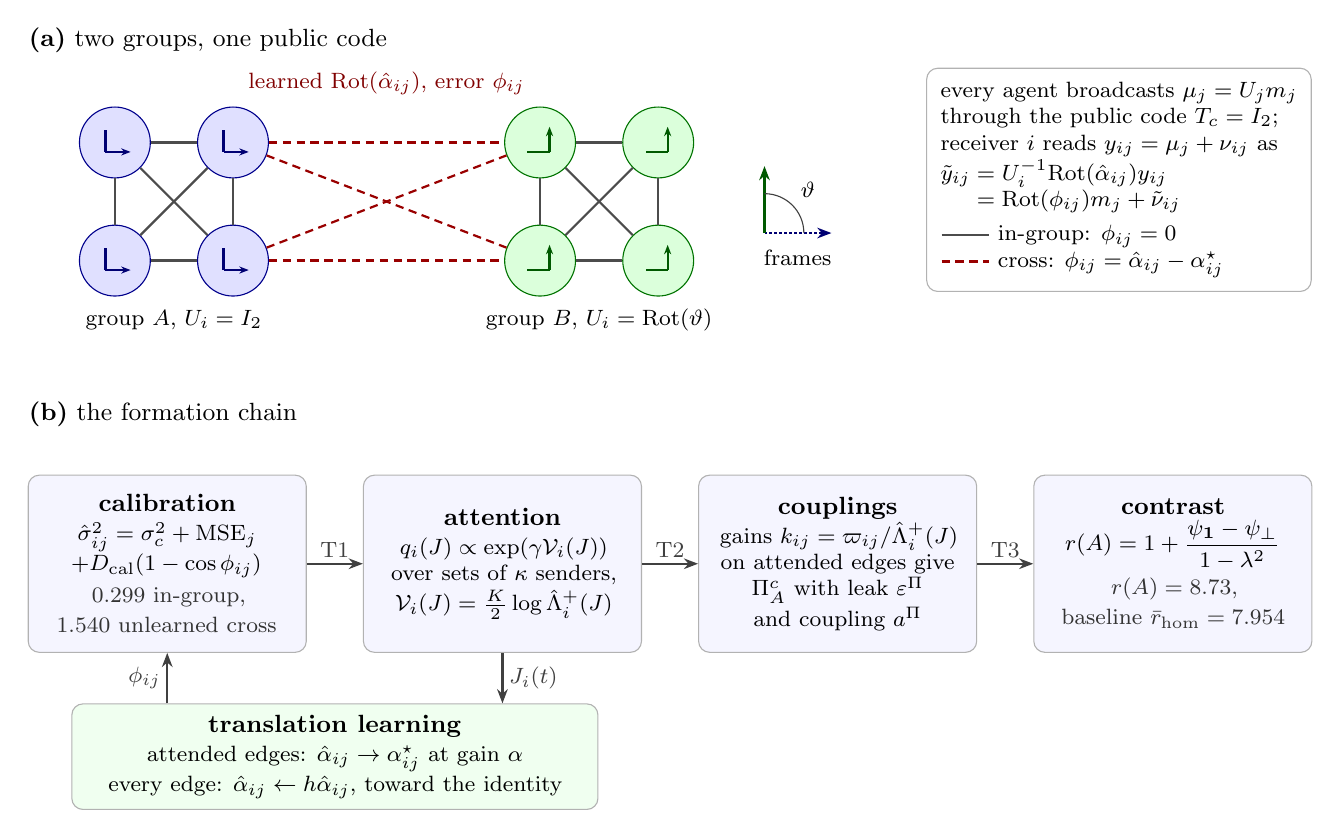
\begin{tikzpicture}[>={Stealth[length=1.8mm]}, every node/.style={font=\small},
    agA/.style={circle, draw=blue!55!black, fill=blue!12, inner sep=0pt, minimum size=9mm},
    agB/.style={circle, draw=green!45!black, fill=green!14, inner sep=0pt, minimum size=9mm},
    ing/.style={gray!60!black, thick},
    crs/.style={red!60!black, thick, densely dashed},
    box/.style={draw=gray!60, fill=blue!4, rounded corners=4pt, align=flush center, inner sep=4pt, minimum height=2.25cm, text width=3.25cm},
    link/.style={->, thick, black!75},
    tl/.style={font=\footnotesize, inner sep=1pt}]
  % (a) the two-group model
  \node[anchor=west, inner sep=0pt] at (0,8.3) {\textbf{(a)} two groups, one public code};
  % agents with their private frames (first axis with an arrowhead): U_i = I_2 on A, Rot(vartheta) on B
  \foreach \nm/\x/\y in {a1/1.1/7.0, a2/2.6/7.0, a3/1.1/5.5, a4/2.6/5.5} {
    \node[agA] (\nm) at (\x,\y) {};
    \draw[->, blue!45!black, thick, >={Stealth[length=1.2mm]}] (\x-0.12,\y-0.12) -- ++(0.32,0);
    \draw[blue!45!black, thick] (\x-0.12,\y-0.12) -- ++(0,0.28);
  }
  \foreach \nm/\x/\y in {b1/6.5/7.0, b2/8.0/7.0, b3/6.5/5.5, b4/8.0/5.5} {
    \node[agB] (\nm) at (\x,\y) {};
    \draw[->, green!35!black, thick, >={Stealth[length=1.2mm]}] (\x+0.12,\y-0.12) -- ++(0,0.32);
    \draw[green!35!black, thick] (\x+0.12,\y-0.12) -- ++(-0.28,0);
  }
  % in-group edges: exact translations
  \foreach \u/\v in {a1/a2, a3/a4, a1/a3, a2/a4, a1/a4, a2/a3, b1/b2, b3/b4, b1/b3, b2/b4, b1/b4, b2/b3}
    \draw[ing] (\u) -- (\v);
  % cross edges: learned rotation with error
  \foreach \u/\v in {a2/b1, a4/b3, a2/b3, a4/b1}
    \draw[crs] (\u) -- (\v);
  \node[font=\footnotesize, red!50!black] at (4.55,7.75) {learned $\mathrm{Rot}(\hat\alpha_{ij})$, error $\phi_{ij}$};
  \node[font=\footnotesize] at (1.85,4.75) {group $A$, $U_i=I_2$};
  \node[font=\footnotesize] at (7.25,4.75) {group $B$, $U_i=\mathrm{Rot}(\vartheta)$};
  % the frames differ by a rotation
  \coordinate (fo) at (9.35,5.85);
  \draw[->, blue!45!black, thick, densely dotted] (fo) -- ++(0.85,0);
  \draw[->, green!35!black, thick] (fo) -- ++(0,0.85);
  \draw[gray!50!black] ($(fo)+(0.5,0)$) arc[start angle=0, end angle=90, radius=0.5];
  \node[font=\footnotesize] at ($(fo)+(0.55,0.55)$) {$\vartheta$};
  \node[font=\footnotesize] at ($(fo)+(0.42,-0.32)$) {frames};
  % message model
  \node[draw=gray!60, fill=white, rounded corners=4pt, anchor=north east, align=left, font=\footnotesize, inner sep=5pt] (msg) at (16.3,7.95)
    {every agent broadcasts $\mu_j=U_jm_j$\\
     through the public code $T_c=I_2$;\\
     receiver $i$ reads $y_{ij}=\mu_j+\nu_{ij}$ as\\
     $\tilde y_{ij}=U_i^{-1}\mathrm{Rot}(\hat\alpha_{ij})y_{ij}$\\
     $\phantom{\tilde y_{ij}}=\mathrm{Rot}(\phi_{ij})m_j+\tilde\nu_{ij}$\\[3pt]
     \tikz[baseline=-0.6ex]\draw[gray!60!black, thick] (0,0) -- (0.6,0); in-group: $\phi_{ij}=0$\\
     \tikz[baseline=-0.6ex]\draw[red!60!black, thick, densely dashed] (0,0) -- (0.6,0); cross: $\phi_{ij}=\hat\alpha_{ij}-\alpha^\star_{ij}$};
  % (b) the formation chain
  \node[anchor=west, inner sep=0pt] at (0,3.55) {\textbf{(b)} the formation chain};
  \node[box] (cal) at (1.765,1.65) {\textbf{calibration}\\[1pt]{\footnotesize $\hat\sigma^2_{ij}=\sigma_c^2+\mathrm{MSE}_j$\\$+D_{\mathrm{cal}}(1-\cos\phi_{ij})$\\[2pt]\color{gray!40!black}$0.299$ in-group,\\$1.540$ unlearned cross}};
  \node[box] (att) at (6.022,1.65) {\textbf{attention}\\[1pt]{\footnotesize $q_i(J)\propto\exp(\gamma\mathcal V_i(J))$\\over sets of $\kappa$ senders,\\$\mathcal V_i(J)=\tfrac K2\log\hat\Lambda^+_i(J)$}};
  \node[box] (cpl) at (10.279,1.65) {\textbf{couplings}\\[1pt]{\footnotesize gains $k_{ij}=\varpi_{ij}/\hat\Lambda^+_i(J)$\\on attended edges give\\$\Pi^c_A$ with leak $\varepsilon^\Pi$\\and coupling $a^\Pi$}};
  \node[box] (con) at (14.536,1.65) {\textbf{contrast}\\[1pt]{\footnotesize $r(A)=1+\dfrac{\psi_{\one}-\psi_\perp}{1-\lambda^2}$\\[2pt]\color{gray!40!black}$r(A)=8.73$,\\baseline $\bar r_{\mathrm{hom}}=7.954$}};
  \node[box, text width=6.4cm, minimum height=1.3cm, fill=green!6] (lrn) at (3.894,-0.8) {\textbf{translation learning}\\[1pt]{\footnotesize attended edges: $\hat\alpha_{ij}\to\alpha^\star_{ij}$ at gain $\alpha$\\every edge: $\hat\alpha_{ij}\leftarrow h\hat\alpha_{ij}$, toward the identity}};
  \draw[link] (cal) -- node[tl, above=1pt] {T1} (att);
  \draw[link] (att) -- node[tl, above=1pt] {T2} (cpl);
  \draw[link] (cpl) -- node[tl, above=1pt] {T3} (con);
  \draw[link] (att.south) -- node[tl, right=1pt] {$J_i(t)$} (att.south |- lrn.north);
  \draw[link] (cal.south |- lrn.north) -- node[tl, left=1pt] {$\phi_{ij}$} (cal.south);
\end{tikzpicture}

  \caption{\textbf{The two-group model and the formation chain.} (a) Two groups of four agents keep their beliefs in private frames, $U_i=I_2$ on $A$ and $U_i=\mathrm{Rot}(\vartheta)$ on $B$ (drawn at $\vartheta=\pi/2$), and broadcast them in full through one public code. Each receiver translates a message with a learned angle: in-group edges are read exactly, and cross edges carry the translation error $\phi_{ij}=\hat\alpha_{ij}-\alpha^\star_{ij}$, whose modulus is $\vartheta$ at the declared start. (b) The chain, with the clauses (T1) to (T3) of \cref{def:frm-target} on its links. C1g calibration turns the error into extra message noise $D_{\mathrm{cal}}(1-\cos\phi_{ij})$ (\cref{lem:frm-calibration}); attention draws sets of $\kappa$ senders from a softmax at policy precision $\gamma$ over their believed values; translation learning corrects only attended edges while every edge relaxes toward the identity, so attention and learning reinforce each other (\cref{thm:frm-formation}); at the split the attended edges fix the gains of the level-0 errors and with them the leak $\varepsilon^\Pi$ and coupling $a^\Pi$ of the world-conditional precision (\cref{lem:frm-split-law}), which give the contrast of each group (\cref{thm:frm-split-contrast}). Gray numbers are at the base point of \cref{sec:frm-model}: calibrated noise $0.299$ on an in-group edge and $1.540$ on an unlearned cross edge, and contrast $8.73$ against the baseline $7.954$.}
  \label{fig:frm-chain}
\end{figure}
% src: figure supplied with the section; base-point numbers of lem:frm-calibration, thm:frm-split-contrast and chk:frm-baseline

\Cref{fig:frm-chain} shows the model and the chain that the rest of this section follows, from calibration through attention and translation learning to the couplings of the world-conditional precision and the contrast of each group. In the notation of \cref{def:fw-translation}, the translation $\Theta_{ij}=\mathrm{Rot}(\hat\alpha_{ij})$ induces the code model $\hat H_{ij}=T_c\Theta_{ij}^{-1}U_i$, so $\tilde y_{ij}=\hat H_{ij}^{-1}y_{ij}$, and the mistranslation $\Upsilon_{ij}=\mathrm{Rot}(\phi_{ij})=\hat H_{ij}^{-1}H_j$ is the identity exactly when $\Theta_{ij}=U_iU_j^{-1}$; it is the rotation error of the static model of \cref{def:coh-calibration-model}. Messages are read at level 0 with assigned noise $\hat R_{ij}=\hat\sigma^2_{ij}I_2$ (\cref{def:fw-levels}), learning is the steady-gain form of the grounded estimator of \cref{prop:fw-rls} with forgetting toward the identity, and each round is a step of the level-0 network of \cref{def:fw-level0} with $W_{ij}=Fk_{ij}\Upsilon_{ij}$. The prior errors $e_i=m_i-\eta$ obey
\begin{equation}\label{eq:frm-error}
e_i(t+1)=F\Bigl[k^0_ie_i(t)+k^s_iv_i(t)+\sum_{j\in J_i(t)}k_{ij}\bigl(\mathrm{Rot}(\phi_{ij})e_j(t)+(\mathrm{Rot}(\phi_{ij})-I)\eta_t+\tilde\nu_{ij}(t)\bigr)\Bigr]-w_t.
\end{equation}
The term $(\mathrm{Rot}(\phi_{ij})-I)\eta_t$ is the mistranslation forcing. Calibration matches its variance but not its correlation with $\eta_t$, so receivers choose senders under a model that misreads the joint structure of messages and world (\cref{sec:mis}).

After the first round, row-sum contraction and the uniform form of the moment bound (M) of \cref{asm:sca-standing} hold on every path of \eqref{eq:frm-error} (Supplement, \cref{rem:frm-moment-bound}).

Besides the full model we use the frozen-slow model, in which the translation errors, the attention law and the claimed prior variance are held fixed and the stationary second moments of \eqref{eq:frm-error} solve a finite linear system, and the mean-field map of \cref{sec:frm-meanfield} for the slow variables. Numbers refer to the base point $F=0.99$, $Q=1-F^2$ (so $P_0=1$), $R^s=1$, $R_c=0.05$, $n=4$, $\kappa=3$, $\vartheta=\pi/2$, $\alpha=0.1$ and $h=0.995$, with $\sigma_\alpha^2=0.01$ in simulations.

\subsection{Calibration converts frame mismatch into message noise}\label{sec:frm-calibration}

Withdrawal needs a receiver's model to register mistranslation, which C0 receivers cannot do (\cref{prop:coh-c0-blind}). C1g calibration registers it as extra message noise, whose size is set by how well the sender tracks the world.

\begin{lemma}[Calibrated mistranslation in the dynamic network]\label{lem:frm-calibration}
Suppose the stationary joint law of $(e_j(t),\eta_t)$ is invariant under rotations and reflections of the plane. For a receiver that reads sender $j$ with translation error $\phi$, the C1g calibrated noise is
\begin{equation}\label{eq:frm-calibration}
\hat\sigma^2_{ij}=R_c+\mathrm{MSE}_j+D_{\mathrm{cal}}(1-\cos\phi),\qquad D_{\mathrm{cal}}=2\Cov_1(\eta_t,m_j(t)),
\end{equation}
where $\mathrm{MSE}_j$ is the per-coordinate mean-square error of $m_j$ and $\Cov_1$ a covariance of one coordinate; for a random error independent of everything else, $\cos\phi$ is replaced by $\E\cos\phi$. At the split, where each group attends only its own members with exact translations and all members have sensing gain $k^s$, the hypothesis holds and
\begin{equation*}
D_{\mathrm{cal}}=\frac{2QF^2k^s}{(1-F^2)(1-\lambda F)},\qquad\lambda=F(1-k^s).
\end{equation*}
\end{lemma}
% src: B2-L1 (extends L3-T4 to the AR(1) level-0 network); checked C2-5
Proof in \cref{app:frm}. A sender whose belief does not track the world has nothing to rotate, so at the split $D_{\mathrm{cal}}$ vanishes with the sensing gain; this is the dynamic form of the withdrawal threshold of \cref{thm:coh-withdrawal}. The in-group value $\hat\sigma^2_{\mathrm{in}}=R_c+\mathrm{MSE}$ is a fixed point, since the error depends on the gains and the gains on the calibration (\cref{thm:frm-split-contrast}(d)). At the base point $\hat\sigma^2_{\mathrm{in}}=0.29872$ and $D_{\mathrm{cal}}=1.24123$, so an unlearned cross edge carries calibrated noise $1.53995$, about five times the in-group value (\cref{chk:frm-calibration}).

\begin{assumption}[Mean-field reduction]\label{asm:frm-mean-field}
(a) Frozen calibration: calibrated precisions are $\varpi_{\mathrm{in}}=1/\hat\sigma^2_{\mathrm{in}}$ on in-group edges and $\varpi_\times(\phi)=1/(\hat\sigma^2_{\mathrm{in}}+D_{\mathrm{cal}}(1-\cos\phi))$ on cross edges, with $\hat\sigma^2_{\mathrm{in}}$, $D_{\mathrm{cal}}>0$ and $\Lambda_0$ held at their values at the split. (b) Closure: in the learning recursion the attention indicator is replaced by its conditional probability given the slow state. (c) Agents are identical apart from their frames, and capacity is scarce, $\kappa\le n-1$.
\end{assumption}
% src: B2 assumptions I5, I6, I8, I9

Part (b) is exact for the conditional mean of the learning recursion. Part (a) is accurate on the split branch, which self-consistent calibration moves only in the fourth digit (\cref{obs:frm-thresholds}).

\subsection{Attention bounds and the mean-field theorem}\label{sec:frm-meanfield}

This subsection proves the population form of the bistability of \cref{prop:frm-bistability}, with explicit thresholds in the policy precision. Fix a receiver $i\in A$; group $B$ is symmetric. In-group translations start exact and stay exact in the mean field. A cross edge starts at $\phi_{ij}=\vartheta$, and its bias fraction $x_j=\phi_{ij}/\vartheta$ is $1$ when unlearned and $0$ when learned. Under \cref{asm:frm-mean-field} the attention frequencies $\mathsf p_j(x)=q_i(\{J:j\in J\})$ depend only on the receiver's own state $x=(x_j)_{j\in B}\in[0,1]^n$, receivers decouple, and the learning rule gives $x(t+1)=\Phi(x(t))+\alpha\mathsf u(t)$, with $\mathsf u(t)$ a martingale difference of conditional variance at most $\frac14+\sigma_\alpha^2/\vartheta^2$ on $[0,1]^n$ and (\cref{app:frm})
\begin{equation}\label{eq:frm-meanfield}
\Phi_j(x)=h\bigl(1-\alpha\mathsf p_j(x)\bigr)x_j+1-h=x_j+\alpha h\bigl[\mathsf p^\ast(1-x_j)-\mathsf p_j(x)x_j\bigr],\qquad\mathsf p^\ast=\frac{1-h}{\alpha h}.
\end{equation}
A fixed point has $x_j=\mathsf p^\ast/(\mathsf p^\ast+\mathsf p_j(x))$: an edge attended at the learning threshold $\mathsf p^\ast$, where forgetting balances learning, is half learned. A cross edge is learned when $x_j<\frac12$ and unlearned when $x_j>\frac12$, and a configuration is split if every cross edge is unlearned, merged if every one is learned, and bridged otherwise. Passing from the stochastic recursion to $\Phi$ as $\alpha\to0$ with $\mathsf p^\ast$ fixed is the business of the ordinary-differential-equation method of stochastic approximation \citep{benaim1999dynamics,kushner1997stochastic}; we do not carry it out (\cref{open:frm-closure}). The analysis uses three constants of the frozen calibration, a lower bound $\Delta\mathcal V(x)$ on the believed value gained when a cross edge of bias fraction $x$ in an attended set is replaced by an in-group edge, the largest difference $\Delta\mathcal V_{\max}$ between the believed values of two sets, and a Lipschitz constant $\mathcal L$ of the set values,
\begin{equation*}
\Delta\mathcal V(x)=\frac K2\log\Bigl(1+\frac{\varpi_{\mathrm{in}}-\varpi_\times(x\vartheta)}{\Lambda_0+\kappa\varpi_{\mathrm{in}}}\Bigr),\qquad\Delta\mathcal V_{\max}=\frac K2\log\frac{\Lambda_0+\kappa\varpi_{\mathrm{in}}}{\Lambda_0+\kappa\varpi_\times(\vartheta)},\qquad\mathcal L=\frac K2\frac{D_{\mathrm{cal}}\vartheta}{(\hat\sigma^2_{\mathrm{in}})^2\Lambda_0}.
\end{equation*}

\begin{lemma}[Attention bounds]\label{lem:frm-attention}
Let $\kappa\le n-1$, $\gamma\ge0$, $\vartheta\in(0,\pi]$ and $x\in[0,1]^n$.
\begin{enumerate}
\item[(a)] $\mathsf p_j(x)\le\bar{\mathsf p}(x_j)$, where $\bar{\mathsf p}(y)=\kappa e^{-\gamma\Delta\mathcal V(y)}/(1+\kappa e^{-\gamma\Delta\mathcal V(y)})$ depends only on the edge's own state.
\item[(b)] $\underline{\mathsf p}\le\mathsf p_j(x)\le\min\{1,\kappa e^{\gamma\Delta\mathcal V_{\max}}/(2n-1)\}$ with $\underline{\mathsf p}=\kappa e^{-\gamma\Delta\mathcal V_{\max}}/(2n-1)$.
\item[(c)] $\sum_{j'\in B}\vert\partial\mathsf p_j/\partial x_{j'}\vert\le2\gamma\mathcal Ln\mathsf p_j(x)$.
\end{enumerate}
\end{lemma}
% src: B2-L3; checked C2-4
Proof in \cref{app:frm}. By (a) an edge less than half learned is attended at most at rate $\bar{\mathsf p}(\frac12)$, whatever the receiver's other edges do. The bound of (a) is attained to six digits in the limit $x_j\to0$ at $\gamma\ge160$; it is not attained at larger $x_j$, because $\Delta\mathcal V$ bounds the value gap from below, and at $x_j=\frac12$ the largest ratio $\mathsf p_j/\bar{\mathsf p}(x_j)$ computed is $0.79$ (\cref{chk:frm-attention}).

\begin{theorem}[Mean field of attention and learning]\label{thm:frm-formation}
Under \cref{asm:frm-mean-field} with $0<\mathsf p^\ast<1$, consider $\Phi$ on $[0,1]^n$ and the thresholds
\begin{equation}\label{eq:frm-thresholds}
\gamma_S=\frac{1}{\Delta\mathcal V(\frac12)}\log\frac{\kappa(1-\mathsf p^\ast)}{\mathsf p^\ast},\qquad\gamma_M=\frac{1}{\Delta\mathcal V_{\max}}\log\frac{\kappa}{(2n-1)\mathsf p^\ast}.
\end{equation}
\begin{enumerate}
\item[(a)] Declared start. The symmetric subspace $\{x_1=\dots=x_n\}$ is invariant. On it $\mathsf p_j=\mathsf P(x)$ with $\mathsf P$ nonincreasing, the reduced map $g(x)=h(1-\alpha\mathsf P(x))x+1-h$ is nondecreasing, and the iterates from the declared start $x=1$ decrease monotonically to the largest fixed point $\bar x$ of $g$, the least-learned fixed point. Fixed points solve $x\mathsf P(x)=\mathsf p^\ast(1-x)$. If $\gamma_S<\gamma<\infty$, then $\bar x>\frac12$ and $\mathsf P(\bar x)<\mathsf p^\ast$: from the declared start the mean field reaches the split branch.
\item[(b)] Global split. Let $\underline x$ be the smallest fixed point in $[0,1]$ of the comparison map $\bar g(y)=h(1-\alpha\bar{\mathsf p}(y))y+1-h$. If (i) $\underline x>\frac12$, equivalently $y\bar{\mathsf p}(y)<\mathsf p^\ast(1-y)$ for $y\in[0,\frac12]$, and (ii) $2\gamma\mathcal Ln\bar{\mathsf p}(x')<\mathsf p^\ast$ for some $x'\in(\frac12,\underline x)$, then $\Phi$ has exactly one fixed point. It is symmetric, lies in $[\underline x,1]^n$, has cross attention at most $\bar{\mathsf p}(\underline x)$, and attracts every initial condition in $[0,1]^n$. Condition (i) holds whenever $\gamma>2\kappa^2/(e\mathsf c_{\mathcal V}\mathsf p^{\ast2})$, with an explicit constant $\mathsf c_{\mathcal V}>0$ given in the proof, and (i) and (ii) both hold for all sufficiently large $\gamma$. Hence the threshold $\gamma_T$, the infimum of the $\gamma'$ such that (i) and (ii) hold for every $\gamma\ge\gamma'$, is finite, and $\gamma_T=O(\mathsf p^{\ast-2})$ as $\mathsf p^\ast\to0$ with the other constants fixed. Conversely, with $\mathsf m_\kappa=\max_{\mathsf t\ge0}\kappa\mathsf te^{-\mathsf t^2}/(1+\kappa e^{-\mathsf t^2})$, attained at $\mathsf t_\kappa$, and $\mathsf c^+_{\mathcal V}=K\vartheta^2D_{\mathrm{cal}}/(4(\hat\sigma^2_{\mathrm{in}})^2(\Lambda_0+\kappa\varpi_{\mathrm{in}}))$, condition (i) fails at $\gamma=\mathsf m_\kappa^2/(\mathsf c^+_{\mathcal V}\mathsf p^{\ast2})$ whenever $\mathsf p^\ast\le\mathsf m_\kappa/(2\mathsf t_\kappa)$, so that $\gamma_T\ge\mathsf m_\kappa^2/(\mathsf c^+_{\mathcal V}\mathsf p^{\ast2})$ there: $\gamma_T$ is of exact order $\mathsf p^{\ast-2}$.
\item[(c)] Merged state. Every trajectory satisfies $\limsup_tx_j(t)\le\mathsf p^\ast/(\mathsf p^\ast+\underline{\mathsf p})$. For $\gamma<\gamma_M$ every cross edge is eventually learned: only merged states exist.
\item[(d)] Local stability. At a symmetric fixed point $\bar x$ let $\mathsf p'_{\mathrm{self}}=\partial\mathsf p_j/\partial x_j$ and $\mathsf p'_{\mathrm{cross}}=\partial\mathsf p_j/\partial x_{j'}$ for $j'\ne j$. Then $\mathsf p'_{\mathrm{self}}\le0$, and the Jacobian of $\Phi$ has the symmetric multiplier $g'(\bar x)\ge0$ and the $(n-1)$-fold symmetry-breaking multiplier $h(1-\alpha\mathsf P(\bar x))-\alpha h\bar x(\mathsf p'_{\mathrm{self}}-\mathsf p'_{\mathrm{cross}})$; the fixed point is linearly stable if and only if both have modulus below one.
\item[(e)] Top-$\kappa$ attention. At $\gamma=\infty$ the split $x=1$ is the only fixed point, and every trajectory converges to it.
\end{enumerate}
\end{theorem}
% src: B2-T1 (extends and in part replaces L3-P16); verdict C2-4 (holds as a theorem about the frozen-calibration mean-field map); repair (iv): sign of the cross derivative only computed; explicit bound on gamma_T added in the proof
Proof in \cref{app:frm}. Below $\gamma_M$ exploration teaches every cross translation, above $\gamma_S$ the declared start reaches the split branch, and above $\gamma_T$ the map has a single fixed point, on the split branch, which attracts every state. Since $\gamma_S$ grows like $\log(1/\mathsf p^\ast)$ and $\gamma_T$ is of exact order $\mathsf p^{\ast-2}$ by (b), slow forgetting widens the window between them, in which the outcome depends on history. Part (d) leaves the sign of $\mathsf p'_{\mathrm{cross}}$ open; it is nonnegative at every computed fixed point, so the stability classes of \cref{tab:frm-thresholds} rest on computed multipliers.

The theorem concerns the frozen-calibration mean-field map, and the step from the full model to the map is open (\cref{open:frm-closure}); what it does and does not establish about formation is collected in \cref{sec:frm-status}.

At the base point $\gamma_M=6.84$ and $\gamma_S=68.2$, the symmetric fixed points form a merged and a split branch joined by an unstable middle branch through folds at $\gamma=60.05$ and $105.9$, the merged branch loses stability to symmetry-breaking perturbations at $\gamma=87.9$, and $\gamma_T$, computed by bisection, is $242.1$ (a numerical observation; Supplement, \cref{obs:frm-thresholds,tab:frm-thresholds,fig:frm-phase}). Off the symmetric subspace the map has stable bridged fixed points, in which a receiver keeps some of its cross edges learned and attended; at the base point they are found for $43.4<\gamma<241.0$ (a numerical observation; Supplement, \cref{obs:frm-bridged}).

\subsection{The world-conditional law at the split and its contrast}\label{sec:frm-contrast}

Attention alone does not make collectives: whether the cut at the split produces them depends on the world-conditional precision of the errors.

Contrast follows the conventions of \cref{def:col-contrast}; at finite $\gamma$, where the conditional covariance depends on the world path, it is computed from $\Sigma^c=\E[\Cov(e(t)\mid\eta)]$ (Supplement, \cref{rem:frm-conventions}).

\begin{lemma}[The world-conditional law at the split]\label{lem:frm-split-law}
Let $\gamma=\infty$, $\kappa\le n-1$, in-group translations exact and cross translation errors nonzero, so that each receiver attends a uniformly random set of $\kappa$ members of its own group. Let all members have sensing gain $k^s$, message gain $\bar k$ and prior weight $k^0$, put $\lambda=F(1-k^s)$, $\mathsf p_{\mathrm{in}}=\kappa/(n-1)$ and $q=F^2((k^s)^2R^s+\kappa\bar k^2R_c)$, and
\begin{equation*}
\psi_\perp=F^2\bigl[(k^0)^2-2k^0\bar k\mathsf p_{\mathrm{in}}+\bar k^2(\kappa-(n-2)\mathsf p_{\mathrm{in}}^2)\bigr],\qquad\psi_{\one}-\psi_\perp=nF^2\bar k\mathsf p_{\mathrm{in}}\bigl(2k^0+(n-2)\bar k\mathsf p_{\mathrm{in}}\bigr)>0.
\end{equation*}
Then the two groups are conditionally independent given the world path, and the world-conditional covariance of the errors of group $A$ is $\Sigma^c_A=(\mathsf s_0I+\mathsf s_1\one\one^\top)\otimes I_2$ with
\begin{equation*}
\mathsf s_0=\frac{q}{1-\psi_\perp},\qquad\mathsf s_1=\mathsf s_0\frac{\psi_{\one}-\psi_\perp}{n(1-\lambda^2)},
\end{equation*}
where $0\le\psi_\perp\le\lambda^2<1$. The precision is diffusive, $\Pi^c_A=(\varepsilon^\Pi I+a^\Pi(nI-\one\one^\top))\otimes I_2$ with leak $\varepsilon^\Pi=1/(\mathsf s_0+n\mathsf s_1)$ and coupling $a^\Pi=\mathsf s_1/(\mathsf s_0(\mathsf s_0+n\mathsf s_1))$ between every pair of members, and the per-coordinate mean-square error is $\mathrm{MSE}=Q/(1-\lambda^2)+\mathsf s_0+\mathsf s_1$. For $\kappa=n-1$ the law is Gaussian, $\psi_{\one}=\lambda^2$ and $\psi_\perp=\lambda_\perp^2$ with $\lambda_\perp=F(k^0-\bar k)$.
\end{lemma}
% src: B2-L2; checked C2-5; repair (ii) declared in rem:frm-conventions
Proof in \cref{app:frm}; checked in \cref{chk:frm-split-law}. Here $\psi_{\one}$ and $\psi_\perp$ are the eigenvalues of $\E[W(t)W(t)^\top]$ on the uniform vector and its complement; for $\kappa=n-1$ the lemma is an instance of the normal case of \cref{thm:col-diffusive-precision}. The comparison medium of \cref{def:col-baseline} is the same population without frame mismatch, each receiver attending $\kappa$ of the other $2n-1$ agents uniformly at random with exact translations and its own calibration fixed point; $\varepsilon^h$ and $a^h$ are its leak and coupling. This is clause (c) of \cref{def:col-baseline} for couplings generated by a declared mechanism, here attention under a budget; the exchangeable population with the split's own mean coupling and leak would give a lower baseline at every point of the grid of \cref{obs:frm-grid}, and under both comparisons the split is a collective at all $162$ points (\cref{sec:col-contrast}).

\begin{theorem}[Contrast at the split and the baseline]\label{thm:frm-split-contrast}
Under the hypotheses of \cref{lem:frm-split-law}:
\begin{enumerate}
\item[(a)] Each group has contrast
\begin{equation}\label{eq:frm-contrast}
r(A)=1+\frac{\psi_{\one}-\psi_\perp}{1-\lambda^2}=1+\frac{nF^2\bar k\mathsf p_{\mathrm{in}}(2k^0+(n-2)\bar k\mathsf p_{\mathrm{in}})}{1-F^2(1-k^s)^2},\qquad r(A)=\frac{1-\lambda_\perp^2}{1-\lambda^2}\text{ for }\kappa=n-1.
\end{equation}
A subset $S\subset A$ with $2\le\vert S\vert=n_S\le n-1$ has $r(S)=(\varepsilon^\Pi+n_Sa^\Pi)/(\varepsilon^\Pi+(n-n_S)a^\Pi)$, every region meeting both groups has $r\le1$, and $A\cup B$ has $r=1$. With $r_{\mathrm{sub}}=(\varepsilon^\Pi+(n-1)a^\Pi)/(\varepsilon^\Pi+a^\Pi)$, which equals $1$ for $n=2$, every region other than $A$ and $B$ has contrast at most $\max\{r_{\mathrm{sub}},1\}$.
\item[(b)] In the comparison medium every region of $n_C<2n$ members has contrast $(\varepsilon^h+n_Ca^h)/(\varepsilon^h+(2n-n_C)a^h)$, increasing in $n_C$, and the whole population has $1+2na^h/\varepsilon^h$. Hence the baseline of \cref{def:col-baseline} is $\bar r_{\mathrm{hom}}=1+2na^h/\varepsilon^h$, attained by the whole population, while $r_{\mathrm{hom}}(n)=1$.
\item[(c)] For every level $r_0$ with $\max\{r_{\mathrm{sub}},\bar r_{\mathrm{hom}}\}<r_0\le r(A)$ the level is admissible, and the collectives at level $r_0$ are exactly $A$ and $B$.
\item[(d)] At every parameter point the C1g calibration condition $\hat\sigma^2_{\mathrm{in}}=R_c+\mathrm{MSE}(\hat\sigma^2_{\mathrm{in}})$ has a solution in $(R_c,\infty)$, and so does that of the comparison medium.
\item[(e)] Let both calibration roots be nondegenerate at a point $(F,Q,R^s,R_c)$ at which, evaluated at these roots, $\max\{r_{\mathrm{sub}},\bar r_{\mathrm{hom}}\}<r_0<r(A)$. Then there are continuous branches of nondegenerate roots on a neighborhood of the point along which the same inequalities hold. The set of such points is open.
\end{enumerate}
\end{theorem}
% src: B2-T2 restated under decision 11 (C2-5 repair: baseline = sup over all sizes incl. whole population); (c) via B1-D3; (e) the gamma = infinity part of B2-T2(d) with nondegeneracy made a hypothesis (repair (v))
Proof in \cref{app:frm}. Contrast grows with the per-member message weight $n\bar k\mathsf p_{\mathrm{in}}$ and falls with the leak $1-F^2(1-k^s)^2$, set by world decorrelation and grounding. Because the finite comparison population is itself a region, the baseline is strict: at the base point $r(A)=8.7329$, $r_{\mathrm{sub}}=2.3182$ and $\bar r_{\mathrm{hom}}=7.954$, so the admissible window is $(7.954,8.733]$ and the significance $r(A)/\bar r_{\mathrm{hom}}$ is $1.098$ (\cref{chk:frm-baseline}), as in \cref{rem:col-baseline-conventions}. In the model of \cref{def:frm-two-group} the hypothesis of exact in-group translations holds from the declared start exactly when $\sigma_\alpha^2=0$. For $\sigma_\alpha^2>0$ attended in-group angles fluctuate, the group contrasts at the base point are about $2$ percent higher (\cref{obs:frm-stochastic}), the comparison medium with noisy learned translations is not computed, and the admissible window is then not established; for $\kappa<n-1$ the attended in-group set also need not be uniformly random, since idealized calibration at the current error ranks in-group senders by $\lvert\phi_{ij}\rvert$.

The weaker convention that compares a region only with regions of its own size is not used, for the reason given in the Supplement (\cref{rem:frm-matched-baseline}). Two numerical observations are reported there. On a grid of 162 parameter points with $\kappa=n-1$, both calibration roots are nondegenerate and $r_{\mathrm{sub}}<\bar r_{\mathrm{hom}}<r(A)$ at every point, so that every admissible window is nonempty (\cref{obs:frm-grid}). In the frozen-slow model with self-consistent calibration at the base point, the split branch at $\gamma=80$, $120$ and $160$ has group contrast $8.6763$, $8.7317$ and $8.7329$, and at $\gamma=80$ only $A$ and $B$ exceed $7.954$ (\cref{obs:frm-exploration}). Openness at finite $\gamma$ is a sketch with an unproved step (\cref{rem:frm-open}).

\subsection{Nulls and the order parameter}\label{sec:frm-nulls}

Clause (T4) asks whether a population in which communication is deleted, frozen or rearranged would select the split too.

\begin{proposition}[Nulls at the split]\label{prop:frm-nulls}
Let reading noise be specific to each receiver.
\begin{enumerate}
\item[(a)] Under label-preserving deletion, renormalized deletion and the frozen-environment null ($\mathfrak N_{\mathrm{lp}}$, $\mathfrak N_{\mathrm{rn}}$ and $\mathfrak N_{\mathrm{fr}}$ of \cref{tab:agy-nulls}), the order parameter $\Omega_{\mathrm{int}}$ of \cref{def:agy-order-parameter} vanishes for every pair. Under the two deletion nulls, and under the frozen-environment null when the initial states that frozen messages carry are deterministic or added to the conditioning set, the world-conditional precision is block diagonal in agents and every region has contrast at most one.
\item[(b)] At the split of \cref{lem:frm-split-law}, $\Omega_{\mathrm{int}}$ vanishes for every pair of agents from different groups. For $\kappa=n-1$ it is positive for every pair from the same group over every window of at least two rounds.
\item[(c)] Consequently, at every level of \cref{thm:frm-split-contrast}(c) the split selects exactly $A$ and $B$, while the deletion nulls, and the frozen-environment null under the condition of (a), select no region.
\end{enumerate}
\end{proposition}
% src: B2-P2(a),(c); uses B4-P5 (prop:agy-nulls-vanish) and L2-P18; condition on the frozen initial states added (prop:agy-nulls-vanish(a) gives block diagonality given the shared drive, which contains the initial state)
Proof in \cref{app:frm}. The condition in (a) matters only for the freezing null. A frozen message delivers its sender's initial state in every round, so that input never washes out, and when the initial states are random and left out of the conditioning set, receivers that read the same sender share it: the law given the world path alone is then not block diagonal, although the law given the shared drive, which contains the initial state, is (\cref{prop:agy-nulls-vanish}(a)), and $\Omega_{\mathrm{int}}$ still vanishes. Differing from these nulls is necessary for any claim of interaction and is achieved by any communication at all (\cref{prop:agy-nulls-vanish}). The decisive comparisons are computed.

At the base point, partner randomization at the matched rate of $\kappa$ partners per round, with cross translations unlearned or learned at the null's attention rate, leaves no region above $7.954$ and has $\Omega_{\mathrm{int}}>0$ across groups (a numerical observation; Supplement, \cref{obs:frm-partner,tab:frm-nulls}). The Supplement also places these comparisons within \cref{def:agy-nulls}: $\mathfrak N_{\mathrm{eff}}$ and $\mathfrak N_{\mathrm{inf}}$ are not applicable, the habit null coincides with partner randomization redrawn every round with learned translations, for which the test of \cref{prop:agy-tests}(b) rejects at level $\alpha_{\mathrm{pr}}$ when $n_{\mathrm{null}}\ge1/\alpha_{\mathrm{pr}}-1$, and partner randomization drawn once and the test on contrasts estimated from finite samples are not computed.

The explanation nulls limit attribution: the code null predicts the frame classes $\{A,B\}$, so under \cref{def:agy-nulls} the split above $\gamma_T$ is code aligned, that is, predictable from the codes alone (Supplement, \cref{sup:frm-explanation-nulls-and-merged-regimes}).

\subsection{Reachability}\label{sec:frm-reach}

\Cref{thm:frm-formation} gives reachability for the mean field. Two numerical observations test how far it carries to the stochastic model.

\begin{observation}[The full model with idealized calibration]\label{obs:frm-stochastic}
The full model at the base point, with eight replicates per cell over 8000 rounds, gives \cref{tab:frm-stochastic}. From the declared start every replicate ends on the split branch at $\gamma=80$, inside the bistable window, and at $\gamma=160$, with cross attention per edge at most $2.1\times10^{-3}$, less than one learned bridge would contribute. At $\gamma=40$ from both starts and at $\gamma=80$ from the declared start the averages agree with the mean field within $5$ percent. At $\gamma=160$ from the declared start the average $1.3\times10^{-6}$ is a single attended cross edge-round among the $8\times3000\times32=768{,}000$ counted, so it agrees with the mean-field value $9\times10^{-7}$ in order of magnitude only. From a merged start at $\gamma=80$ the population settles in partially bridged states, with averages $(0.254,0.569)$ against the merged fixed point $(0.344,0.127)$ of the map: the stochastic model at $\alpha=0.1$ leaves a fixed point that is linearly stable for the map, with multipliers $0.9762$ and $0.9937$ (\cref{chk:frm-thresholds}). Replica estimates of the world-conditional covariance (isotropic part) at $\gamma=160$ give group contrasts from $8.86$ to $9.00$, about $2$ percent above the value $8.733$ that \cref{lem:frm-split-law} gives for exact in-group translations. The excess is the effect of in-group angle noise, which that lemma does not include: at $\sigma_\alpha^2=0.01$ an attended in-group translation angle fluctuates with stationary standard deviation $h\alpha\sigma_\alpha/(1-h^2(1-\alpha)^2)^{1/2}=0.022$ radians. With noiseless angle observations, $\sigma_\alpha^2=0$, the estimated contrasts are $8.741$ and $8.699$ (\cref{chk:frm-stochastic}).
\end{observation}
% src: B2-X2; C2-4 independent slow-recursion simulation

\begin{table}[t]
\centering
\caption{The full stochastic model with idealized calibration against the mean field: cross attention per edge and mean bias fraction of cross edges, averaged over eight replicates and the last 3000 of 8000 rounds.}
\label{tab:frm-stochastic}
\begin{tabular}{@{}lllll@{}}
\toprule
$\gamma$ & start & cross attention & bias fraction & mean field \\
\midrule
40 & declared & $0.392$ & $0.116$ & merged; $0.395$, $0.113$ \\
40 & merged & $0.392$ & $0.116$ & merged \\
80 & declared & $1.85\times10^{-3}$ & $0.965$ & split branch; $1.8\times10^{-3}$, $0.966$ \\
80 & merged & $0.254$ & $0.569$ & merged branch; $0.344$, $0.127$ \\
160 & declared & $1.3\times10^{-6}$ & $1.000$ & split; $9\times10^{-7}$, $1.000$ \\
160 & merged & $0.025$ & $0.960$ & split, with bridges up to $\gamma_T$ \\
\bottomrule
\end{tabular}
\end{table}

\begin{observation}[Online calibration from a symmetric start]\label{obs:frm-online}
Replace idealized calibration by an exponential average, at rate $\alpha_{\mathrm{cal}}$, of the grounded residuals $\frac12\Vert\tilde y_{ij}-\eta_t\Vert^2$ on attended rounds, frozen when the edge is unattended and started at $R_c+\mathrm{MSE}$, so that attention is initially uniform. A run ends in the split's attention pattern when every cross edge ends with $\vert\phi_{ij}\vert\ge0.3\vartheta$. This cutoff for a learned cross edge is stricter than the bias fraction $\frac12$ that classifies edges for the map (\cref{sec:frm-meanfield}): an edge with bias fraction between $0.3$ and $\frac12$ counts as unlearned here, so the counts are upper bounds on those at the cutoff $\frac12$. \Cref{tab:frm-online} counts such replicates after 6000 rounds, eight per cell, and a rerun with other seeds and 8000 rounds at $\alpha_{\mathrm{cal}}=0.05$ gives 6, 1 and 2 of 8 at $\gamma=160$, $400$ and $1600$. Reruns of a single cell differ by up to three replicates: at $\gamma=400$, $\alpha_{\mathrm{cal}}=0.05$ the table, the rerun and the separate run described next give 0, 1 and 3 of 8. This is the size of most differences between cells, so the counts establish that for $\gamma\ge160$ the pattern is reached in some replicates and missed in others, and little about its dependence on the parameters beyond the largest differences. In a separate run at $\gamma=400$, $\alpha_{\mathrm{cal}}=0.05$, contrasts from the isotropic part of the local-error covariance given the realized attention (sampling error about 10 percent) lie between $2.4$ and $7.6$ for the groups, nine of ten below $5.1$, and between $1.9$ and $3.7$ for the union in the five replicates ending with two or three cross edges below $0.3\vartheta$. The pattern is not a contrast criterion: one replicate ends in it with group contrasts $3.69$ and $4.06$ and union contrast $3.58$ (\cref{chk:frm-online}).
\end{observation}
% src: B2-X3 with repair (iii): nine of ten below 5.1; replicate 7 (gamma = 400, alpha_r = 0.05) has no learned cross edge but contrasts 3.69, 4.06, union 3.58; estimator from B2_sim3 (local part given realized attention, half-trace reduction)

\begin{table}[t]
\centering
\caption{Online calibration from a symmetric start: replicates out of eight that end in the split's attention pattern (every cross edge with $\vert\phi_{ij}\vert\ge0.3\vartheta$, a cutoff below the bias fraction $\frac12$ that separates learned from unlearned edges for the map, so the counts are upper bounds on those at $\frac12$) after 6000 rounds. The counts come from eight replicates per cell, and reruns of single cells differ by up to three replicates (\cref{chk:frm-online}).}
\label{tab:frm-online}
\begin{tabular}{@{}lllll@{}}
\toprule
$\gamma$ & $\alpha_{\mathrm{cal}}=0.02$ & $0.05$ & $0.2$ & $0.5$ \\
\midrule
80 & 0 & 0 & 0 & 0 \\
160 & 2 & 3 & 7 & 1 \\
400 & 0 & 0 & 5 & 0 \\
\bottomrule
\end{tabular}
\end{table}

Early uniform attention lets cross translations be learned before calibration registers the mismatch, and calibration noise acts as exploration; this mechanism and the dependence of the counts on $\alpha_{\mathrm{cal}}$, which is not monotone at $\gamma=160$, are discussed in the Supplement (\cref{sup:frm-reachability-in-the-full-model}).

\subsection{What fails, and the grounding tension}\label{sec:frm-fails}

Each failure marks a hypothesis the positive results need. Low policy precision and C0 receivers leave every cross translation learned, under the conditions stated in the Supplement (\cref{sup:frm-explanation-nulls-and-merged-regimes}). Two failures are structural.

The first is abundant capacity: if $\kappa\ge n$, every receiver attends at least $\kappa-n+1$ cross senders in every round at every $\gamma$, so no attention cut separates the groups (Supplement, \cref{prop:frm-capacity}). The second is exact translation.

\begin{proposition}[Exact translation removes the mechanism]\label{prop:frm-exact-fusion}
Let every receiver know the mistranslation $\Upsilon_{ij}=\mathrm{Rot}(\phi_{ij})$ of every message, the part of class C2 that concerns translations (with $T_c=I_2$ the identifiable subspace is the whole plane), and keep everything else, including C1g calibration of the corrected messages.
\begin{enumerate}
\item[(a)] A corrected message has the joint law with $(\eta,e)$ of a correctly translated message, and its calibrated noise $R_c+\mathrm{MSE}_j$ does not depend on the receiver.
\item[(b)] In every state of this null and at every $\gamma\in[0,\infty]$, a receiver attends a sender of higher calibrated precision at least as often as one of lower precision. Hence each of the $n$ receivers outside the group of a sender $j_1$ of largest precision attends the cross sender $j_1$ with probability at least $\kappa/(2n-1)$.
\item[(c)] Let the start law of the belief states $(m_i-\eta,\hat P^-_i)_{i}$ given the world path be invariant under all permutations of the $2n$ agents, as it is at the declared start with identical initial beliefs, and as it is whenever the start and the initial world state $\eta_0$ are jointly independent of the innovations $w_t$ and the law of the start given $\eta_0$ is invariant, and let idealized calibration be evaluated on the law of the errors at the current round. Then at every time and every $\gamma\in[0,\infty]$ all senders have the same calibrated precision, every receiver attends a uniformly random set of $\kappa$ senders, and the law of the errors given the world path is invariant under all permutations of the $2n$ agents. Contrast therefore depends only on the size of a region, and at no level are $A$ and $B$ the selected regions. A stationary state of this trajectory is the comparison medium of \cref{thm:frm-split-contrast}(b), in which no region is selected at any admissible level.
\end{enumerate}
From such a start law the split does not survive this translation-aware null.
\end{proposition}
% src: B2-P4; decision 12; C2 2.3(b); part (b) added by the editor (receiver-independent calibration makes all receivers rank senders alike)
Proof in \cref{app:frm}. Knowing the translation error removes the cost side of the withdrawal inequality \eqref{eq:coh-withdrawal}. What is proved is therefore that the split fails the translation-aware form of the exact-fusion persistence clause, and under that reading the split is attributed to misreading joint structure, not to communication as action. States of this null that are not exchangeable, which other start laws could reach, are not classified; by (b) each of them has $n$ cross edges attended at rate at least $\kappa/(2n-1)$ at every $\gamma$, whereas on the split branch of the mean-field map cross attention is at most $\bar{\mathsf p}(\frac12)$ per edge and vanishes as $\gamma\to\infty$ (\cref{lem:frm-attention}(a)). For full cross-covariance-aware exact fusion in this model, the null $\mathfrak N_{\mathrm{ex}}$ of \cref{tab:agy-nulls}, whose receivers also model the correlation of each message's error with their own, the conclusion is heuristic and uncomputed: cross messages carry errors independent of the receiver's own local error, while in-group messages share the group's collective fluctuation, so cross messages would be preferred. Complementary access would keep a cross edge attended (\cref{ex:coh-unique-information}), a case the model excludes (\cref{open:frm-access}). A single receiver at the base point that fuses exactly against the split's stationary law was computed to value sets of senders more highly the more cross senders they contain, which confirms the heuristic for one unilateral deviation (\cref{obs:hie-exact-receiver}); the population law under full exact fusion is open (\cref{open:hie-exact-fusion-population}). At $\gamma=\infty$ and $\kappa=n-1$, a pragmatic preference for coordinated exchange, which every null keeps, lets the split survive the translation-aware null at any strength, but the surviving split is then the declared code partition, not formation (\cref{rem:hie-pragmatic}).

For $\kappa=n-1$, weak grounding tends to raise the split contrast while it weakens the withdrawal signal $D_{\mathrm{cal}}$ that forms the cut, so that high-contrast collectives of weakly grounded members need higher policy precision to form; this is the grounding tension of \cref{thm:coh-grounding-tension} seen from the formation side (Supplement, \cref{rem:frm-grounding}).

\subsection{Status and conjectures}\label{sec:frm-status}

Against \cref{def:frm-target}, with idealized C1g calibration, identical agents and $\kappa\le n-1$, clauses (T1) and (T2) hold once calibration registers mistranslation (\cref{lem:frm-calibration}); (T3) holds at $\gamma=\infty$, the map's unique fixed point, with exact in-group translations, $\sigma_\alpha^2=0$, at the levels of the window of \cref{thm:frm-split-contrast}(c), and with openness given nondegenerate roots and a nonempty window (\cref{thm:frm-split-contrast}(e)), and at finite $\gamma$ by computation and a sketch (Supplement, \cref{obs:frm-exploration,rem:frm-open}), while for $\sigma_\alpha^2>0$ in-group angle noise raises the group contrasts by about $2$ percent at the base point (\cref{obs:frm-stochastic}) and the admissible window is not computed; (T4) holds for the applicable differ nulls, by proof for the deletion and freezing nulls (\cref{prop:frm-nulls}; for the freezing null when its initial states are deterministic or conditioned on) and by computation at the base point for partner randomization redrawn every round (Supplement, \cref{obs:frm-partner}), with which the habit null coincides, while partner randomization drawn once is not computed, and fails for the survive null from a start law exchangeable given the world path, by proof in its translation-aware form (\cref{prop:frm-exact-fusion}) and heuristically for full cross-covariance-aware exact fusion; (T5) holds for the map (\cref{thm:frm-formation}) and in every replicate of the full model with idealized calibration (\cref{obs:frm-stochastic}).

Hence, in the two-group model at $\gamma=\infty$ with $\sigma_\alpha^2=0$, clauses (T1) to (T3) and (T5) are theorems, the contrast clause (T3) at the levels of the window of \cref{thm:frm-split-contrast}(c), which is nonempty at every computed parameter point (Supplement, \cref{obs:frm-grid}), and the declared start is then itself the split (\cref{thm:frm-formation}(e), \cref{thm:frm-split-contrast}). For $\gamma_S<\gamma<\infty$ reachability of the split branch is a theorem about the frozen-calibration mean-field map (\cref{thm:frm-formation}(a),(b)), with the stochastic-approximation step from the full model to the map open (\cref{open:frm-closure}), and the contrast of the reached state is computed at the base point (Supplement, \cref{obs:frm-exploration}). Clause (T4) fails for the translation-aware null of type S from a start law that is exchangeable given the world path, as the declared start with identical initial beliefs is, so from such a start the model yields no formation result in the sense of \cref{def:frm-target}. Formation there is a calibration-level effect of misreading joint structure, hypothesis H3 in its calibration form and hypothesis H2 read as misreading: receivers that know their translation errors pay no mistranslation cost, so from a start law exchangeable given the world path the model's collectives fail the translation-aware form of the exact-fusion persistence clause of the null family, as \cref{prop:frm-exact-fusion} proves, while for full cross-covariance-aware exact fusion in this model the conclusion is heuristic; above $\gamma_T$ they coincide with the code partition. Persistence under exact fusion with drifting frames is a conjecture (Supplement, \cref{conj:frm-drifting-frames}). Online calibration from a symmetric start reaches the split's attention pattern (not necessarily a split selected by contrast) in 0 to 7 of 8 replicates per cell, with reruns of a cell differing by up to three replicates, and is open (\cref{obs:frm-online}; Supplement, \cref{open:frm-online}). Formation beyond this model is a conjecture (\cref{conj:frm-formation}). Persistence under exact fusion is the obligation that would change this verdict most.

It is conjectured that when the group frames drift, the frame angles of $A$ and $B$ performing independent random walks, the split survives the exact-fusion null on an open set of parameters (Supplement, \cref{conj:frm-drifting-frames}).

\begin{conjecture}[Formation beyond the two-group model]\label{conj:frm-formation}
Consider level-0 agents in a stationary linear-Gaussian world with private linear frames, public codes, C1g or C1i calibration, grounded translation learning with forgetting on attended edges, capacity $\kappa$ and attention selected by expected free energy at precision $\gamma$. Let their frames fall into classes such that capacity can be filled within classes and every cross-class edge, read through its unlearned translation, has calibrated precision below that of the $\kappa$th best sender of the receiver's class. Then there are thresholds $0<\gamma_-\le\gamma_+<\infty$, depending on the learning and forgetting rates, such that on an open set of parameters: for $\gamma>\gamma_+$ the stochastic dynamics converge from the declared start law, with probability tending to one as the learning gains vanish, to configurations whose attended subgraph consists of asymptotically flat components separated by unattended cuts, each a collective at every level of a nonempty admissible window; for $\gamma<\gamma_-$ exploration removes every cut; and for $\gamma_-<\gamma<\gamma_+$ split, bridged and merged configurations coexist and the realized one depends on history.
\end{conjecture}
% src: L3-C1 as refined by B2-X1 (bridged states added); L2-O3; decision 12 (formation beyond the model is a conjecture)
What is established of the conjecture in the two-group model, what would refute it, and a conjectured route to formation that does not rest on misreading are discussed in the Supplement (\cref{sup:frm-remarks-on-the-formation-conjecture}).

\begin{openproblem}[Stochastic closure]\label{open:frm-closure}
Prove that the recursion $x(t+1)=\Phi(x(t))+\alpha\mathsf u(t)$ of the two-group model tracks the mean-field map on finite horizons as $\alpha\to0$ with $\mathsf p^\ast$ fixed, a constant-gain stochastic approximation with state-dependent attention noise, and estimate the escape times from the split and from bridged states between $\gamma_S$ and $\gamma_T$. At the base-point gain $\alpha=0.1$ the tracking is not quantitative inside the bistable window: from a merged start at $\gamma=80$ the full model leaves the linearly stable merged fixed point of the map for partially bridged states (\cref{obs:frm-stochastic}, \cref{tab:frm-stochastic}).
\end{openproblem}
% src: B2-O1

Three further problems are open (Supplement, \cref{open:frm-online,open:frm-self-consistent,open:frm-access}): conditions under which online calibration reaches the split from the symmetric start with probability tending to one as the gains vanish; the extension of \cref{thm:frm-formation}(b) to the self-consistent mean field along whole trajectories; and the extension of the analysis to anisotropic access, heterogeneous senders and groups on a graph with geometry.

\section{Scale}\label{sec:sca}
% src: L4 (all); R1 to R3 (dennis2026communicating); B3 Sections 1, 2, 5; B5 Section 1; B1-P3, B1-P6; L6-P5, L6-P8, L6-F14, L6-F16; L7-M12, L7-P2 to L7-P4, L7-C1; critic V9 to V11, C3, D7; C2 repairs for sca

Hypothesis H4 says that the informational correlation length and time grow with the scale of collectives: media that carry messages farther, such as the telephone, or keep them longer, such as archives and international organizations, support larger and longer-lived collectives. This section turns that sentence into statements with hypotheses. It defines the correlation length $\xi$ and the correlation time $\tau$; the second-moment length $\xi_2$, contrast and the largest extent $\Lstar$ come from \cref{sec:col}. Every statement concerns world-conditional errors, because a shared world correlates all agents whether or not they communicate (Supplement, \cref{prop:sca-world-conditioning}).

The results fall into two classes. Light cones need only locality: under any local rule, attention chosen by expected free energy included, influence travels at most one hop per round, and agents more than $2t$ hops apart are independent after $t$ rounds. Every length, time and volume needs the moment bound \textup{(M)} and a named contraction of the error dynamics. The agents' own attention can violate \textup{(M)} (Supplement, \cref{ex:sca-amplifying-profile}), and then only the finite-time statements of \cref{sec:sca-lightcone,sec:sca-nomoment} survive. The section ends with H4 in final form (\cref{thm:sca-h4}).

\subsection{Hypotheses and when they fail}\label{sec:sca-hypotheses}

Different members of the scale theory need different hypotheses, so we name them once.

\begin{assumption}[Standing setting and hypothesis labels]\label{asm:sca-standing}
Agents $i\in V$ occupy the vertices of the potential communication graph $\mathcal G=(V,\mathcal E)$, with hop distance $d(i,j)$, maximal degree $\Delta$ and hop length $\ell$. The connected part $e(t)=(e_i(t))_{i\in V}$ of the agents' errors (\cref{lem:fw-common-mode}) obeys
\begin{equation}\label{eq:sca-recursion}
e(t+1)=W(t)e(t)+\zeta(t),
\end{equation}
where $W(t)$ is the error-transfer matrix of the level-0 network (\cref{def:fw-level0}) for the attention schedule of round $t$, and the local noise $\zeta(t)$ is independent across rounds with covariance $Q^\zeta(t)$; channel noise shared by several receivers is conditioned on, as in \cref{def:col-world-conditional}. Given the world path, $e(t)$ is the fluctuation of the errors about their conditional mean, so $\Sigma(t)=\Cov(e(t))$ is their world-conditional covariance, written $\Sigma^c$ in \cref{prop:col-world-conditional}, and $\Sigma$ denotes its stationary value when one exists. Block norms are spectral norms. The hypothesis labels are the following.
\begin{itemize}
\item[\textup{(Lin)}] The schedule $(W(t))_t$ is independent of the noises and of $e(0)$: it is exogenous, or chosen from deterministic quantities such as claimed covariances.
\item[\textup{(G)}] The noises and the initial law are Gaussian.
\item[\textup{(B)}] The noise is local: $Q^\zeta(t)$ is block diagonal over agents, with blocks between $q_{\min}I$ and $qI$.
\item[\textup{(Loc)}] $W_{ij}(t)\neq0$ only if $i=j$ or $(i,j)\in\mathcal E$.
\item[\textup{(M)}] The moment bound, in two forms. Stationary form: a stationary world-conditional law of $e$ with finite second moments exists. Uniform form: the agents' errors $m_i(t)-\eta_t$ have second moments bounded uniformly in $i$ and $t$, for a schedule that may vary in time and depend on the states. Unqualified, \textup{(M)} means the stationary form.
\item[\textup{(C$_r$)}] Row-sum contraction: $\lambda=\sup_t\max_i\sum_j\Vert W_{ij}(t)\Vert<1$.
\item[\textup{(C$_{rc}$)}] $\lambda_r\lambda_c<1$, where $\lambda_r=\lambda$ and $\lambda_c$ is the analogous supremum of block column sums.
\item[\textup{(C$_\rho$)}] Spectral contraction: $W$ is time invariant and $\Vert W^k\Vert_2\le K_Af^k$ for all $k\ge0$, for some $f<1$ and $K_A\ge1$; such constants exist exactly when $\rho(W)<1$.
\item[\textup{(N)}] Normality with isotropic noise ($WW^\top=W^\top W$ and $Q^\zeta=qI$), or reversibility ($WQ^\zeta=Q^\zeta W^\top$).
\item[\textup{(TI)}] Translation invariance on $\Z^D$ or on a ring.
\item[\textup{(NN)}] $W(t)\ge0$ entrywise.
\end{itemize}
\end{assumption}
% src: B3-D1; M_spec decision 16; the uniform form of (M) is the form L7-P4 (prop:min-grounding-moment) delivers

The next lemma relates the contractions; we write $\Phi(t,s)=W(t-1)\cdots W(s)$ and $\Phi(t,t)=I$.

\begin{lemma}[Relations among the hypotheses]\label{lem:sca-relations}
\begin{enumerate}
\item[(a)] Under \textup{(Lin)}, \textup{(C$_r$)} and block-diagonal noise with blocks $\preceq qI$, $\sum_j\Vert\Phi_{ij}(t,s)\Vert\le\lambda^{t-s}$ for every schedule. If in addition the initial errors $m_k(0)-\eta_0$ are independent of the schedule and have second moments bounded uniformly in $k$, $\sup_i\Vert B^{\mathrm{mis}}_i\Vert<\infty$, the world innovation has second moments bounded uniformly in time and, where codes are mistranslated, the world is stationary with finite second moments, then \textup{(M)} holds in uniform form. \textup{(M)} holds in stationary form when $W$ and the law of $\zeta(t)$ are time invariant; under \textup{(G)} the latter means a time-invariant $Q^\zeta$. If the schedule depends on the states, the population is finite with $N$ agents, every realized $W(t)$ obeys the bound of \textup{(C$_r$)}, and the initial errors and the inputs of the error recursion (local noise, world innovation and any mistranslation term) have second moments bounded uniformly, then the row-sum bound holds pathwise and \textup{(M)} holds in uniform form, with root-mean-square errors bounded by a constant that grows like $N^{1/2}$.
\item[(b)] \textup{(C$_{rc}$)} implies $\Vert W(t)\Vert_2\le(\lambda_r\lambda_c)^{1/2}<1$ for every $t$, hence \textup{(C$_\rho$)} when $W$ is time invariant.
\item[(c)] Let $W$ be time invariant and let $W$ and $Q^\zeta\succ0$ be bounded on $\ell^2(V)$, with $\rho(W)$ the spectral radius there. Then $\rho(W)<1$ implies \textup{(M)}. On a finite population the converse holds, so \textup{(M)} holds if and only if $\rho(W)<1$. On an infinite population the converse can fail. For scalar agents on $\Z^D$ under \textup{(TI)} with a summable kernel, $Q^\zeta=qI$ and symbol $\hat W(p)=\sum_xW_{0x}e^{\mathrm ip\cdot x}$, \textup{(M)} holds if and only if
\begin{equation}\label{eq:sca-fourier-moment}
\int_{[-\pi,\pi]^D}\frac{\mathrm dp}{1-|\hat W(p)|^2}<\infty,
\end{equation}
the integrand being read as $+\infty$ where $|\hat W(p)|\ge1$, and the stationary solution $\sum_{n\ge0}W^n\zeta(t-1-n)$ then has variance $q$ times the mean of the integrand over $[-\pi,\pi]^D$. The lazy walk on $\Z^3$ with $W_{xx}=1/4$ and $W_{xy}=1/8$ for $|x-y|=1$ has $\rho(W)=1$ and satisfies \eqref{eq:sca-fourier-moment}, with variance $1.4395q$; its analogues on $\Z$ and $\Z^2$ violate \eqref{eq:sca-fourier-moment}.
\end{enumerate}
\end{lemma}
% src: B3-L1(a)-(c)
Proof in \cref{app:sca}; the lazy-walk variance is computed in \cref{chk:sca-relations}. The hypotheses hold in several classes of populations.

\begin{proposition}[Sufficient conditions]\label{prop:sca-sufficient}
\begin{enumerate}
\item[(a)] Scalar level-0 receivers. With exact code models and $0\le F\le1$, every attention schedule gives \textup{(NN)} with row sums $F(1-k^s_i(t))$ (\cref{rem:fw-convex-gains}), hence \textup{(C$_r$)} with $\lambda\le F(1-\inf_{i,t}k^s_i(t))$ when the right side is below one, for instance whenever $F<1$. Then, under the moment hypotheses of \cref{lem:sca-relations}(a), \textup{(M)} holds in uniform form for exogenous schedules and, on finite populations, for schedules that depend on the states, and in stationary form for a time-invariant schedule and noise law. \textup{(C$_{rc}$)} can fail, because a sender's column sum grows with its audience.
\item[(b)] One common rank-one code. Under the hypotheses of \cref{prop:min-common-code}(b), which include level-1 receivers that know the codes and read the senders' law headers, symmetric listening, a frozen profile at its covariance fixed point and $F=fI_K$ with $0<f<1$, \textup{(C$_\rho$)} holds with rate $f$ and with $K_A=K_{\tilde M}$, the transient constant of that proposition, hence \textup{(M)}; \textup{(C$_r$)} need not hold.
\item[(c)] Noiseless grounding. Under the hypotheses of \cref{prop:min-grounding-moment} with its contraction factor $\varpi_g<1$, again at level 1, \textup{(M)} holds in uniform form for attention that depends on the past in any way.
\item[(d)] Routing at finite precision. Under the conditions of \cref{prop:sca-routing}(d), on a finite population, the routed dynamics, linear or not, has a unique stationary law, reached at an exponential rate.
\end{enumerate}
\end{proposition}
% src: B3-P1, B3-L1(e) (rem:fw-convex-gains), L7-P2, L7-P3 (prop:min-common-code), L7-P4 (prop:min-grounding-moment), L4-P3(d)
Proof in \cref{app:sca}. Part (b) matters because \textup{(C$_r$)} fails in most random common-code instances (\cref{chk:min-common-code}), so the results that assume it come with spectral versions (Supplement, \cref{prop:sca-spectral}); \cref{sec:min} lists the further conditions for stable mean dynamics derived in \citet{dennis2026communicating}. The hypotheses can fail for the agents' own attention.

In an instance taken from \citet{dennis2026communicating}, with two level-1 receivers and sender-specific codes, the attention profile that expected free energy selects has a frozen mean map with dominant eigenvalue $\rho=1.0613$, so \textup{(M)} fails in both forms (Supplement, \cref{ex:sca-amplifying-profile}). With one common code such amplification is conjectured not to occur, under the conditions stated there; \cref{prop:min-common-code} proves two cases with a rank-one code (Supplement, \cref{conj:sca-common-code}).

\subsection{Light cones}\label{sec:sca-lightcone}

The first constraint on scale needs neither stationarity nor linearity, only that every update is local.

\begin{definition}[Local rules and influence bounds]\label{def:sca-local-rule}
A local rule updates agent $i$ from its closed neighborhood $\mathcal G[i]$, the agent and its neighbors in $\mathcal G$: $\mu_i(t+1)=\mathfrak U^{(t)}_i(\mu_{\mathcal G[i]}(t),\zeta_i(t))$, with noises $\zeta_i(t)$ independent across agents and rounds. Given the world path, and with noise shared by several receivers conditioned on, this form covers messages, attention chosen from what an agent holds, and reads of records or other written external states once these are made vertices of $\mathcal G$. A matrix $\bar J\ge0$ with $\bar J_{ik}=0$ for $k\notin\mathcal G[i]$ is an influence bound if $\Vert\partial_k\mathfrak U^{(t)}_i\Vert\le\bar J_{ik}$ for all rounds, states and noises. We write $J_{ij}(t,s)=\partial\mu_i(t)/\partial\mu_j(s)$, $g_{\mathrm{tot}}=\max_i\sum_k\bar J_{ik}$ and, for $\varphi\ge0$, $g_\varphi=\max_i\sum_k\bar J_{ik}e^{\varphi d(i,k)}$.
\end{definition}
% src: L4-D1, L4-D2 (D_ij and C renamed J_ij and J_bar, L4-D2's kappa dropped); the general rule is stated here, as Section 2 directs; the map is written mathfrak U because Upsilon_ij is the mistranslation of def:fw-translation and mathcal U names the ultrametric contrast and intervention sets elsewhere

\begin{theorem}[Light cone]\label{thm:sca-lightcone}
\begin{enumerate}
\item[(a)] For $s\le t$, $\mu_i(t)$ is a measurable function of the states $\mu_k(s)$ with $d(i,k)\le t-s$ and of the noises $\zeta_k(u)$ with $s\le u<t$ and $d(i,k)\le t-1-u$. In particular $J_{ij}(t,s)=0$ when $d(i,j)>t-s$.
\item[(b)] If the initial states $\mu_i(0)$ are world-conditionally independent across agents and independent of the noises, then $\mu_i(t)$ and $\mu_j(t)$ are world-conditionally independent whenever $d(i,j)>2t$, and $\mu_i(t+h)$ and $\mu_j(t)$ whenever $d(i,j)>2t+h$.
\item[(c)] If $\bar J$ is an influence bound, then pathwise $\Vert J_{ij}(t,s)\Vert\le(\bar J^{t-s})_{ij}$, $\sum_j\Vert J_{ij}(t,s)\Vert\le g_{\mathrm{tot}}^{t-s}$, and $\Vert J_{ij}(t,s)\Vert\le e^{-\varphi d(i,j)}g_\varphi^{t-s}$ for every $\varphi\ge0$.
\end{enumerate}
\end{theorem}
% src: R1 (dennis2026communicating), L4-P1, B3-T1(a)
Proof in \cref{app:sca}; checked on a nonlinear ring (\cref{chk:sca-lightcone}). Influence travels at most one hop, a distance $\ell$, per round, as \citet{dennis2026communicating} showed for linear updates. Part (b) gives independence, which is stronger than vanishing covariance, for every local rule; correlations need two cones to overlap, so they spread at twice the influence velocity. These are exact discrete-time counterparts of Lieb--Robinson bounds \citep{lieb1972finite,marchioro1978velocity,raz2009estimating} and of the finite speed at which correlations are generated \citep{bravyi2006lieb}. When $g_\varphi>1$ influence grows inside the cone (\cref{sec:sca-nomoment}). With independent Poisson clocks of rate $\nu$, at whose events agents apply $\mathfrak U_i$, the cone acquires an exponentially small tail.

The bound on the expected influence under such clocks is in the Supplement (\cref{prop:sca-poisson}): with $g=\max_i\sum_{k\neq i}\bar J_{ik}$ and $\bar J_{\mathrm{diag}}=\max_i\bar J_{ii}$ it decays exponentially in $t$ along $d(i,j)\ge vt$ for every $v$ above the velocity $v_{\mathrm{LR}}=\max\bigl\{0,\inf_{\varphi>0}\nu(ge^\varphi+\bar J_{\mathrm{diag}}-1)/\varphi\bigr\}$ hops per unit time.

Attention chosen by expected free energy makes the update depend on beliefs through the choice itself. Let agent $i$ have a finite policy set $\mathcal P_i$, apply $\mathfrak U_{i,\pi}$ under policy $\pi$, and draw $\pi$ from the policy posterior $q_i(\pi\mid\mu)\propto E_i(\pi)e^{-\gamma G_i(\pi;\mu)}$, with habits $E_i$, policy precision $\gamma$ and expected free energy \eqref{eq:fw-efe} evaluated at the current states, independently across agents (sampled routing), or apply $\sum_\pi q_i(\pi\mid\mu)\mathfrak U_{i,\pi}$ (averaged routing). On a convex state domain let $\bar A_{ik}$ bound $\Vert\partial_k\mathfrak U_{i,\pi}\Vert$, let $\mathrm{Lip}_{ik}$ be a Lipschitz constant of $G_i(\pi;\cdot)$ in $\mu_k$, both uniform in $\pi$, and let $\mathrm{osc}_i=\sup_\mu\max_{\pi,\pi'}\Vert\mathfrak U_{i,\pi}(\mu)-\mathfrak U_{i,\pi'}(\mu)\Vert$.

\begin{proposition}[Belief-dependent routing]\label{prop:sca-routing}
Put $\bar J_{ik}(\gamma)=\bar A_{ik}+\tfrac{\gamma}{2}\mathrm{osc}_i\mathrm{Lip}_{ik}$.
\begin{enumerate}
\item[(a)] Averaged routing moves agent $i$'s coordinate by at most $\sum_k\bar J_{ik}(\gamma)\Vert\mu_k-\mu'_k\Vert$ when the state moves from $\mu$ to $\mu'$, so \cref{thm:sca-lightcone}(c) and \cref{prop:sca-poisson} hold with $\bar J(\gamma)$ in place of $\bar J$.
\item[(b)] Sampled routing admits a coupling of two copies started at $\mu(0)$ and $\mu'(0)$ with $\E\Vert\mu_i(t)-\mu'_i(t)\Vert\le\sum_j(\bar J(\gamma)^t)_{ij}\Vert\mu_j(0)-\mu'_j(0)\Vert$ in synchronous rounds.
\item[(c)] $g(\gamma)\le g(0)+\frac{\gamma}{2}\max_i\mathrm{osc}_i\sum_{k\neq i}\mathrm{Lip}_{ik}$, and $v_{\mathrm{LR}}\le eg(\gamma)\nu$ when $\bar J_{ii}(\gamma)\le1$ for all $i$.
\item[(d)] If $g_{\mathrm{tot}}(\gamma)=\max_i\sum_k\bar J_{ik}(\gamma)<1$, the averaged dynamics is a contraction in $\max_i\Vert\cdot\Vert$, and on a finite population with a closed state domain, if every $\mathrm{osc}_i$ is finite and the one-step law of the sampled dynamics from one state, hence from every state, has a finite first moment, the sampled dynamics has a unique stationary law with finite first moment, reached at an exponential rate in the Wasserstein distance. This holds for $\gamma<\gamma_D=\min_i2(1-\sum_k\bar A_{ik})/(\mathrm{osc}_i\sum_k\mathrm{Lip}_{ik})$.
\end{enumerate}
\end{proposition}
% src: L4-P3
Proof in \cref{app:sca}; checked on 300 random instances (\cref{chk:sca-routing}). Part (d) is a contraction condition in the spirit of Dobrushin's uniqueness criterion \citep{dobrushin1968description}. The bound is attained, by a chain that shows a mechanism the linear theory misses.

In that chain each relay attends one of two sources and prefers the one that agrees with what it heard: under averaged routing influence decays geometrically below a threshold of the policy precision and the sign held at the head propagates without decay above it, and under sampled routing with message noise the routing bit has, in a computed case, a correlation length of $21.5$ hops, far beyond that of the continuous content (Supplement, \cref{ex:sca-switch-chain}). At infinite policy precision causality survives and the amplitude bound fails (Supplement, \cref{rem:sca-argmax}).

\subsection{Without the moment bound}\label{sec:sca-nomoment}

\Cref{ex:sca-amplifying-profile} shows that the moment bound can fail. The support statement of \cref{thm:sca-lightcone}(b) needs nothing; the next theorem adds magnitudes without any contraction.

\begin{theorem}[Finite-time clustering without contraction]\label{thm:sca-no-moment}
Assume \textup{(Lin)}, \textup{(B)} and \textup{(Loc)}, and initial errors independent across agents with block covariances $\preceq q_0I$. Let $\bar J_{ik}=\sup_t\Vert W_{ik}(t)\Vert$, an influence bound of the linear recursion, with $g_\varphi$ as above; it may exceed one.
\begin{enumerate}
\item[(a)] For $t\ge1$, $\varphi\ge0$ and $d=d(i,j)$,
\begin{equation}\label{eq:sca-no-moment}
\Vert\Cov(e_i(t),e_j(t))\Vert\le e^{-\varphi d}\Bigl[q\sum_{n=\lceil d/2\rceil}^{t-1}g_\varphi^{2n}+q_0g_\varphi^{2t}\one\{2t\ge d\}\Bigr],
\end{equation}
and, for a lag $h\ge0$, with $(d-h)_+=\max\{d-h,0\}$,
\begin{equation}\label{eq:sca-no-moment-lag}
\Vert\Cov(e_i(t+h),e_j(t))\Vert\le e^{-\varphi d}g_\varphi^h\Bigl[q\sum_{n=\lceil(d-h)_+/2\rceil}^{t-1}g_\varphi^{2n}+q_0g_\varphi^{2t}\one\{2t+h\ge d\}\Bigr].
\end{equation}
The bracket is that of \eqref{eq:sca-no-moment} evaluated at the distance $(d-h)_+$, because the later state $e_i(t+h)$ reads $e(t)$ on a ball of radius $h$ around $i$.
\item[(b)] The top canonical correlation of $e_i(t)$ and $e_j(t)$ is at most $\Vert\Cov(e_i(t),e_j(t))\Vert/q_{\min}$. If $g_\varphi>1$, it is at most $K_\varphi\exp(-\varphi[d-2v_\varphi t])$ with $v_\varphi=\ln g_\varphi/\varphi$ and $K_\varphi=(q/(g_\varphi^2-1)+q_0)/q_{\min}$. Hence the $\theta$-correlation radius $d_\theta(t)$, the largest $d(i,j)$ at which the top canonical correlation of $e_i(t)$ and $e_j(t)$ is at least $\theta$, satisfies
\begin{equation}\label{eq:sca-radius}
d_\theta(t)\le\min\Bigl\{2t,\inf_{\varphi}\Bigl[2v_\varphi t+\varphi^{-1}\ln\frac{K_\varphi}{\theta}\Bigr]\Bigr\},
\end{equation}
the infimum running over all $\varphi>0$ with $g_\varphi>1$.
\item[(c)] If $g_\varphi<1$ for some $\varphi>0$, the bound \eqref{eq:sca-no-moment} is uniform in $t$ and decays at the rate $\varphi+\ln(1/g_\varphi)$ per hop: the stationary clustering regime.
\end{enumerate}
\end{theorem}
% src: B3-T1(b),(c)
Proof in \cref{app:sca}; checked on rings with spectral radius up to $1.33$ (\cref{chk:sca-no-moment}). Without \textup{(M)} there is no time-independent length: by \eqref{eq:sca-radius} the correlated region has radius at most $2v_\varphi t$ plus a constant, so it grows at most at twice the Lieb--Robinson velocity $v_\varphi$ and never faster than two hops per round, while for time-invariant $W$ the variances grow at least like $q_{\min}\rho(W)^{2(t-1)}$ and at most like $g_0^{2t}$. Inside the cone a time-invariant unstable profile does something specific.

Under the hypotheses stated there, a time-invariant $W$ with a simple dominant eigenvalue $\rho>1$ has $\rho^{-2t}\Sigma(t)$ converging to a rank-one matrix, so the top canonical correlation of every pair of agents on which the unstable mode is nonzero tends to one (Supplement, \cref{prop:sca-rank-one}); when the amplification sits at one site of a stable chain, the shared mode advances at less than one hop per round and is never wider than the medium's correlation length (Supplement, \cref{prop:sca-amplifying-site}). We call such an amplifying profile a rumor; it is not a collective, because the definition of a collective includes \textup{(M)} (Supplement, \cref{rem:sca-rumors}).

\subsection{Clustering}\label{sec:sca-clustering}

Under \textup{(M)} the covariance has a decay length. We define the lengths and the time of the theory and then bound them.

\begin{definition}[Correlation length and correlation time]\label{def:sca-lengths}
Let $\Sigma$ be the stationary covariance under \textup{(M)}, or, for an exogenous schedule under \textup{(M)} in uniform form, the covariance $\Sigma(t)$ of the process started in the infinite past, with bounds required uniformly in $t$. Let $R_{ij}=\Sigma_{ii}^{-1/2}\Sigma_{ij}\Sigma_{jj}^{-1/2}$ be its standardized blocks.
\begin{enumerate}
\item[(a)] On an infinite graph the correlation length in hops is $\xi\in[0,\infty]$, defined by
\begin{equation*}
\xi^{-1}=\liminf_{n\to\infty}\Bigl(-\frac1n\ln\sup_{d(i,j)\ge n}\Vert R_{ij}\Vert\Bigr),
\end{equation*}
with $\xi=0$ when the supremum vanishes for all large $n$. The mass is $m=1/\xi$, and the physical correlation length is $\ell\xi$. For families of finite graphs, bounds on $\xi$ mean bounds uniform in $|V|$.
\item[(b)] For scalar agents on $\Z^D$ under \textup{(TI)}, the Ornstein--Zernike length in coordinate direction $d$ is $\xi_{\mathrm{OZ},d}=1/m_d$, where $m_d=-\limsup_{t\to\infty}t^{-1}\ln\sum_{x:x_d=t}\Sigma(x)$ is the decay rate of the covariance summed over hyperplanes.
\item[(c)] For time-invariant $W$ with $\rho(W)<1$, the correlation time is $\tau=-1/\ln\rho(W)$ rounds.
\end{enumerate}
\end{definition}
% src: L4-D5, B1-P3(b)

\begin{theorem}[Exponential clustering]\label{thm:sca-clustering}
Assume \textup{(Lin)}, \textup{(Loc)}, \textup{(C$_r$)} and block-diagonal local noise with blocks $\preceq qI$.
\begin{enumerate}
\item[(a)] $\Phi_{ij}(t,s)=0$ if $d(i,j)>t-s$, and $\sum_j\Vert\Phi_{ij}(t,s)\Vert\le\lambda^{t-s}$.
\item[(b)] Under the moment hypotheses of \cref{lem:sca-relations}(a), \textup{(M)} holds in uniform form, and it holds in stationary form when $W$ and the law of $\zeta(t)$ are time invariant. The covariance $\Sigma(t)=\sum_{n\ge0}\Phi(t,t-n)Q^\zeta(t-1-n)\Phi(t,t-n)^\top$ of the process started in the infinite past satisfies $\Sigma(t)\succeq Q^\zeta(t-1)$ and
\begin{equation}\label{eq:sca-clustering}
\Vert\Sigma_{ij}(t)\Vert\le\frac{q\lambda^{2\lceil d(i,j)/2\rceil}}{1-\lambda^2}\le B_\Sigma e^{-m_\Sigma d(i,j)},\qquad B_\Sigma=\frac q{1-\lambda^2},\quad m_\Sigma=\ln\frac1\lambda.
\end{equation}
\item[(c)] Started at time $s$ from a block-diagonal covariance with blocks $\preceq q_0I$, $\Cov(e(t))$ obeys the same bound plus $q_0\lambda^{2(t-s)}\one\{2(t-s)\ge d(i,j)\}$.
\item[(d)] $\Vert\Cov(e_i(t+h),e_j(t))\Vert\le q\lambda^{\max(h,d(i,j))}/(1-\lambda^2)$.
\end{enumerate}
Under \textup{(B)}, $\lambda_{\min}(\Sigma(t))\ge q_{\min}$ and $\Vert R_{ij}\Vert\le\Vert\Sigma_{ij}\Vert/q_{\min}$, so $\xi\le1/\ln(1/\lambda)$.
\end{theorem}
% src: R2 (dennis2026communicating), L4-P6; constants in the form used by thm:col-markov-bound(c) and app:coh-tension
Proof in \cref{app:sca}. This is the clustering result of \citet{dennis2026communicating}, completed with the initial-condition term and the space-time cone, in the form that \cref{thm:col-markov-bound}(c) uses. In the scalar level-0 network the leak is $\varepsilon_i=1-F+Fk^s_i$ (\cref{def:fw-level0}). The bound is ballistic: its rate $\ln(1/\lambda)\approx\varepsilon$ allows lengths of order $1/\varepsilon$, whereas the exact length on lattices is of order $\sqrt{a/\varepsilon}$ (\cref{thm:sca-oz}). Four results refine it.

They are in the Supplement, each under the hypotheses stated there. With local noise correlated across agents at length $\xi_w$ the decay rate is at least $\min(\ln(1/\lambda),1/\xi_w)$, and identical agents that sense one world without communicating have a diagonal world-conditional covariance while the unconditional correlation of their errors is the same at every distance, which is why every scale bound concerns the world-conditional law (\cref{prop:sca-world-conditioning}). Under \textup{(C$_\rho$)} in place of \textup{(C$_r$)} the covariance decays at least at the rate $\ln(1/f)$ per hop, and under \textup{(B)} $\xi\le\tau$ (\cref{prop:sca-spectral}). When $W(t)$ is dominated in block norm by $\lambda$ times a reversible stochastic matrix supported on the graph, the covariance decays at least at the rate $\vartheta\sqrt{2\ln(1/\lambda)}$ per hop for every $\vartheta\in(0,1)$, the square root characteristic of diffusion (\cref{thm:sca-diffusive}). For heterogeneous nearest-neighbor media on $\Z$ the correlation length is bracketed by the Ornstein--Zernike lengths of two homogeneous media built from the extreme leaks and weights (\cref{prop:sca-heterogeneous}).

\subsection{Ornstein--Zernike decay and the second-moment length}\label{sec:sca-oz}

On lattices with nearest-neighbor attention the covariance can be computed exactly, and it shows that the length of hypothesis H4 is diffusive. Let scalar agents occupy $\Z^D$ under \textup{(TI)} with $W_{ii}=c\ge0$ and $W_{ij}=a>0$ for nearest neighbors, so that $\lambda=c+2Da=1-\varepsilon$ with $\varepsilon>0$, and let $Q^\zeta=qI$. The symbol of $W$ is $\hat W(p)=c+2a\sum_{d=1}^D\cos p_d$ for $p\in[-\pi,\pi]^D$, and its tilted counterpart is $\psi(\boldsymbol\varphi)=c+2a\sum_{d=1}^D\cosh\varphi_d$ for $\boldsymbol\varphi\in\R^D$. For a unit vector $\mathbf u\in\R^D$ let $m(\mathbf u)=\max\{\boldsymbol\varphi\cdot\mathbf u:\psi(\boldsymbol\varphi)\le1\}$, the support function of a compact convex set that contains the origin in its interior.

\begin{theorem}[Ornstein--Zernike decay on $\Z^D$]\label{thm:sca-oz}
In this setting:
\begin{enumerate}
\item[(a)] $\Sigma=q(I-W^2)^{-1}=\tfrac q2[(I-W)^{-1}+(I+W)^{-1}]$, with symbol $\hat\Sigma(p)=q/(1-\hat W(p)^2)$.
\item[(b)] For every $\boldsymbol\varphi$ with $\psi(\boldsymbol\varphi)<1$ and every $x\in\Z^D$, $\Sigma(x)\le qe^{-\boldsymbol\varphi\cdot x}/(1-\psi(\boldsymbol\varphi)^2)$. Hence along every sequence $x\to\infty$ with $x/|x|\to\mathbf u$, $\liminf-\ln\Sigma(x)/|x|\ge m(\mathbf u)$.
\item[(c)] The covariance summed over the hyperplane $\{x_1=t\}$ equals the one-dimensional covariance of part (e) with $c$ replaced by $c+2(D-1)a$. Its decay rate is $m_1=m(\mathbf u_1)$, with $\mathbf u_1$ the first coordinate unit vector, and
\begin{equation}\label{eq:sca-oz-axis}
\cosh m_1=1+\frac{\varepsilon}{2a},\qquad m_1=2\arcsinh\sqrt{\frac{\varepsilon}{4a}}=\sqrt{\frac{\varepsilon}{a}}\Bigl(1-\frac{\varepsilon}{24a}+O(\varepsilon^2)\Bigr),
\end{equation}
in every dimension, so $\xi_{\mathrm{OZ}}=1/\arccosh(1+\varepsilon/(2a))$ in each coordinate direction.
\item[(d)] Along the diagonal $\mathbf u=(1,\dots,1)/\sqrt D$, $m(\mathbf u)=\sqrt D\arccosh(1+\varepsilon/(2Da))=\sqrt{\varepsilon/a}(1-\varepsilon/(24Da)+O(\varepsilon^2))$, so the support function is isotropic to leading order, with relative anisotropy $\tfrac{\varepsilon}{24a}(1-\tfrac1D)+O(\varepsilon^2)$.
\item[(e)] For $D=1$, with $\cosh m=1+\varepsilon/(2a)$ and $\cosh m'=(1+c)/(2a)$,
\begin{equation}\label{eq:sca-oz-1d}
\Sigma(x)=\frac{q}{4a}\Bigl[\frac{e^{-m|x|}}{\sinh m}+(-1)^x\frac{e^{-m'|x|}}{\sinh m'}\Bigr],
\end{equation}
a pure exponential with no power-law prefactor ($m'>m$ when $c>0$). On a ring of even length $N$, $e^{-m|x|}$ is replaced by $\cosh(m(N/2-|x|))/\sinh(mN/2)$, and likewise for $m'$.
\item[(f)] For fixed $c>0$, as $\varepsilon\to0$: $\Sigma(0)\sim q/(4\sqrt{a\varepsilon})$ if $D=1$; $\Sigma(0)=\frac{q}{8\pi a}\ln\frac1\varepsilon+O(1)$ if $D=2$; and $\Sigma(0)$ stays bounded if $D\ge3$.
\item[(g)] $\sum_x|x|^2\Sigma(x)=4Dqa\lambda/(1-\lambda^2)^2$ and $\sum_x\Sigma(x)=q/(1-\lambda^2)$, so the second-moment length is
\begin{equation}\label{eq:sca-xi2-exact}
\xi_2^2=\frac{\sum_x|x|^2\Sigma(x)}{2D\sum_x\Sigma(x)}=\frac{2a\lambda}{1-\lambda^2}=\frac a\varepsilon\cdot\frac{2\lambda}{1+\lambda}.
\end{equation}
\end{enumerate}
\end{theorem}
% src: R3 (dennis2026communicating), L4-T1(a),(b),(d),(e),(f),(g); C2-2 repair (cosh m = 1 + eps/(2a) with lambda = c + 2Da); L4-T1(c) moved to rem:sca-oz-form
Proof in \cref{app:sca}; checked against Lyapunov solutions, Fourier inversion and direct summation (\cref{chk:sca-oz-ring,chk:sca-oz-lattice,chk:sca-lengths}). The ring case of (e) is the third result of \citet{dennis2026communicating}, which writes the rate as $\cosh m=(1-c)/(2a)$, the same number for $D=1$ only. In physical units
\begin{equation}\label{eq:sca-xi-physical}
\ell\xi_{\mathrm{OZ}}=\frac{\ell}{2\arcsinh\sqrt{\varepsilon/(4a)}}\approx\ell\sqrt{\frac a\varepsilon},
\end{equation}
H4's formula, with $a$ the weight on messages and $\varepsilon$ the leak, grounding plus forgetting (\cref{fig:sca-oz}). Distance is hop distance when $\xi$ is a few hops, since for large $\varepsilon/a$ the set $\{\psi\le1\}$ approaches a cube and $m(\mathbf u)\approx|\mathbf u|_1\ln(\varepsilon/a)$, and it becomes Euclidean only when $\xi\gg1$, where the set approaches a ball: the geometry in which a collective lives depends on its scale (\cref{asm:int-a8}). By (f) the world-conditional on-site variance diverges as $\varepsilon\to0$ when $D\le2$ and stays bounded when $D\ge3$; it adds to the shared-error floor $Q/(\varepsilon(2-\varepsilon))$ of the common mode, which diverges in every dimension (\cref{thm:coh-grounding-tension}).

\begin{figure}[t]
  \centering
  % Figure: correlation length on the ring (W_ii=c=0.25, W_ij=a for neighbors, leak eps=1-c-2a).
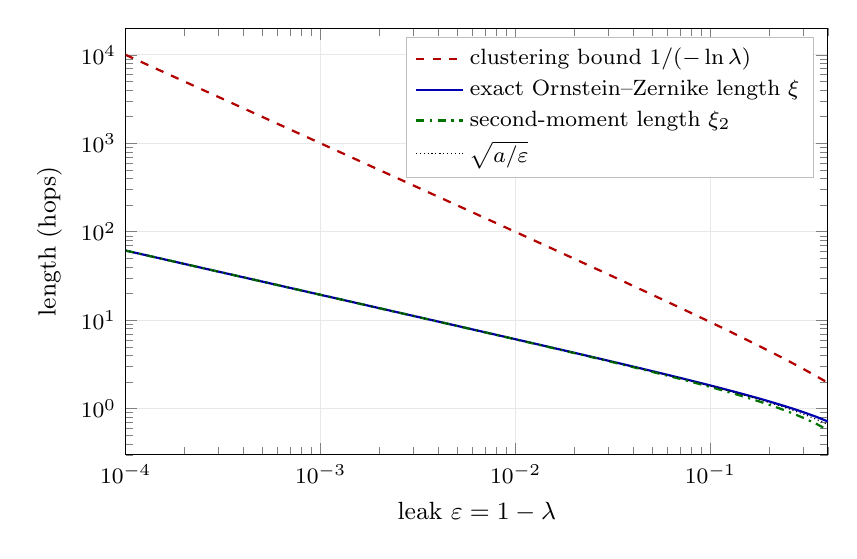
\begin{tikzpicture}
  \begin{loglogaxis}[width=10.5cm, height=7cm,
      xmin=1e-4, xmax=0.4, ymin=0.3, ymax=2e4,
      xlabel={leak $\varepsilon=1-\lambda$}, ylabel={length (hops)},
      grid=major, grid style={gray!18},
      legend style={font=\footnotesize, at={(0.98,0.98)}, anchor=north east, draw=gray!50, fill=white, cells={anchor=west}},
      every axis label/.style={font=\small}, tick label style={font=\footnotesize}]
    \addplot[red!70!black, thick, dashed] coordinates {(0.0001,9999.5) (0.000115094,8688.07) (0.000132466,7548.62) (0.00015246,6558.6) (0.000175472,5698.42) (0.000201957,4951.04) (0.00023244,4301.68) (0.000267524,3737.48) (0.000307904,3247.27) (0.000354378,2821.35) (0.000407867,2451.28) (0.00046943,2129.74) (0.000540284,1850.38) (0.000621834,1607.65) (0.000715692,1396.75) (0.000823717,1213.51) (0.000948047,1054.3) (0.00109114,915.97) (0.00125584,795.781) (0.00144539,691.354) (0.00166356,600.622) (0.00191465,521.789) (0.00220364,453.294) (0.00253625,393.782) (0.00291907,342.074) (0.00335967,297.148) (0.00386677,258.113) (0.00445041,224.198) (0.00512215,194.73) (0.00589527,169.127) (0.00678509,146.881) (0.00780922,127.553) (0.00898793,110.76) (0.0103445,96.1684) (0.0119059,83.4907) (0.013703,72.4756) (0.0157713,62.905) (0.0181518,54.5895) (0.0208916,47.3645) (0.0240449,41.0869) (0.0276742,35.6324) (0.0318512,30.8932) (0.0366588,26.7755) (0.042192,23.1976) (0.0485604,20.0888) (0.05589,17.3875) (0.0643259,15.0403) (0.0740351,13.0007) (0.0852098,11.2283) (0.0980712,9.68808) (0.112874,8.34947) (0.129911,7.186) (0.149519,6.17461) (0.172087,5.29528) (0.198062,4.53055) (0.227957,3.86526) (0.262364,3.28618) (0.301965,2.78175) (0.347543,2.34187) (0.4,1.95762)};
    \addlegendentry{clustering bound $1/(-\ln\lambda)$}
    \addplot[blue!70!black, thick] coordinates {(0.0001,61.2338) (0.000115094,57.0771) (0.000132466,53.2025) (0.00015246,49.5908) (0.000175472,46.2242) (0.000201957,43.0861) (0.00023244,40.1609) (0.000267524,37.4343) (0.000307904,34.8926) (0.000354378,32.5235) (0.000407867,30.315) (0.00046943,28.2564) (0.000540284,26.3375) (0.000621834,24.5487) (0.000715692,22.8813) (0.000823717,21.3269) (0.000948047,19.878) (0.00109114,18.5273) (0.00125584,17.2681) (0.00144539,16.0944) (0.00166356,15.0001) (0.00191465,13.98) (0.00220364,13.0291) (0.00253625,12.1425) (0.00291907,11.3159) (0.00335967,10.5452) (0.00386677,9.82667) (0.00445041,9.1567) (0.00512215,8.53198) (0.00589527,7.94944) (0.00678509,7.40618) (0.00780922,6.89952) (0.00898793,6.42696) (0.0103445,5.98617) (0.0119059,5.57495) (0.013703,5.19129) (0.0157713,4.83327) (0.0181518,4.49914) (0.0208916,4.18723) (0.0240449,3.89601) (0.0276742,3.62403) (0.0318512,3.36993) (0.0366588,3.13247) (0.042192,2.91046) (0.0485604,2.7028) (0.05589,2.50844) (0.0643259,2.32643) (0.0740351,2.15583) (0.0852098,1.9958) (0.0980712,1.8455) (0.112874,1.70417) (0.129911,1.57107) (0.149519,1.44548) (0.172087,1.3267) (0.198062,1.21405) (0.227957,1.10684) (0.262364,1.00433) (0.301965,0.905735) (0.347543,0.810157) (0.4,0.716452)};
    \addlegendentry{exact Ornstein--Zernike length $\xi$}
    \addplot[green!45!black, thick, dashdotted] coordinates {(0.0001,61.2316) (0.000115094,57.0747) (0.000132466,53.1999) (0.00015246,49.5881) (0.000175472,46.2213) (0.000201957,43.083) (0.00023244,40.1576) (0.000267524,37.4307) (0.000307904,34.8888) (0.000354378,32.5193) (0.000407867,30.3106) (0.00046943,28.2516) (0.000540284,26.3323) (0.000621834,24.5432) (0.000715692,22.8753) (0.000823717,21.3206) (0.000948047,19.8712) (0.00109114,18.52) (0.00125584,17.2603) (0.00144539,16.086) (0.00166356,14.9911) (0.00191465,13.9704) (0.00220364,13.0187) (0.00253625,12.1313) (0.00291907,11.3039) (0.00335967,10.5324) (0.00386677,9.81291) (0.00445041,9.14194) (0.00512215,8.51615) (0.00589527,7.93245) (0.00678509,7.38795) (0.00780922,6.87996) (0.00898793,6.40598) (0.0103445,5.96365) (0.0119059,5.55079) (0.013703,5.16536) (0.0157713,4.80545) (0.0181518,4.46928) (0.0208916,4.15519) (0.0240449,3.86162) (0.0276742,3.58712) (0.0318512,3.33032) (0.0366588,3.08995) (0.042192,2.86482) (0.0485604,2.65379) (0.05589,2.45583) (0.0643259,2.26993) (0.0740351,2.09516) (0.0852098,1.93062) (0.0980712,1.77549) (0.112874,1.62895) (0.129911,1.49024) (0.149519,1.3586) (0.172087,1.23331) (0.198062,1.11364) (0.227957,0.998874) (0.262364,0.888254) (0.301965,0.780986) (0.347543,0.676187) (0.4,0.572822)};
    \addlegendentry{second-moment length $\xi_2$}
    \addplot[black, densely dotted] coordinates {(0.0001,61.2332) (0.000115094,57.0764) (0.000132466,53.2017) (0.00015246,49.59) (0.000175472,46.2233) (0.000201957,43.0851) (0.00023244,40.1599) (0.000267524,37.4332) (0.000307904,34.8914) (0.000354378,32.5222) (0.000407867,30.3136) (0.00046943,28.2549) (0.000540284,26.3359) (0.000621834,24.547) (0.000715692,22.8794) (0.000823717,21.325) (0.000948047,19.8759) (0.00109114,18.525) (0.00125584,17.2657) (0.00144539,16.0918) (0.00166356,14.9974) (0.00191465,13.9771) (0.00220364,13.0259) (0.00253625,12.139) (0.00291907,11.3122) (0.00335967,10.5413) (0.00386677,9.82243) (0.00445041,9.15215) (0.00512215,8.5271) (0.00589527,7.9442) (0.00678509,7.40055) (0.00780922,6.89349) (0.00898793,6.42048) (0.0103445,5.97921) (0.0119059,5.56749) (0.013703,5.18327) (0.0157713,4.82466) (0.0181518,4.48989) (0.0208916,4.1773) (0.0240449,3.88534) (0.0276742,3.61255) (0.0318512,3.3576) (0.0366588,3.11921) (0.042192,2.89619) (0.0485604,2.68744) (0.05589,2.49191) (0.0643259,2.30861) (0.0740351,2.13662) (0.0852098,1.97507) (0.0980712,1.82312) (0.112874,1.67997) (0.129911,1.54486) (0.149519,1.41705) (0.172087,1.29581) (0.198062,1.1804) (0.227957,1.07007) (0.262364,0.964008) (0.301965,0.861317) (0.347543,0.760923) (0.4,0.661438)};
    \addlegendentry{$\sqrt{a/\varepsilon}$}
  \end{loglogaxis}
\end{tikzpicture}

  \caption{\textbf{Correlation length on the ring.} For $W_{ii}=c=0.25$ and $W_{ij}=a$ between neighbors, with leak $\varepsilon=1-c-2a$, the exact Ornstein--Zernike length $\xi_{\mathrm{OZ}}=1/\arccosh(1+\varepsilon/(2a))$ and the second-moment length $\xi_2$ both follow $\sqrt{a/\varepsilon}$, while the clustering bound of \cref{thm:sca-clustering} allows lengths up to $1/(-\ln\lambda)\approx1/\varepsilon$.}
  \label{fig:sca-oz}
\end{figure}

\Cref{thm:sca-oz} proves decay at least at the rate $m(\mathbf u)$ in every direction and exact decay of hyperplane sums. That $m(\mathbf u)$ is the exact pointwise rate, with the power-law prefactor of the Ornstein--Zernike form, follows from a theorem on walks with drift that we have read only in restatement, and the constant of the prefactor rests on a heuristic step and is not a result of this manuscript (Supplement, \cref{rem:sca-oz-form}).

The second-moment length $\xi_2$, which bounds the extent of collectives (\cref{thm:col-contrast-size}), never exceeds the Ornstein--Zernike length for translation-invariant diffusive precisions with couplings of finite range, under the hypotheses stated there, and for the medium of \cref{thm:sca-oz} $\xi_2^2\le a/\varepsilon$, so an upper bound stated with $\xi_2$ also holds there with $\xi_{\mathrm{OZ}}$ or $\sqrt{a/\varepsilon}$ (Supplement, \cref{prop:sca-lengths-relation}).

\subsection{Correlation time, diffusive scaling and records}\label{sec:sca-time}

A collective that persists must keep its variables correlated in time, and hypothesis H4 assigns that persistence to memory. The first result bounds how long any linear collective variable stays correlated; the variable may drift, since a collective is a persistent pattern and not a fixed list of coordinates (\cref{asm:int-a10}).

Under \textup{(M)} and \textup{(Lin)} with $W$ and $Q^\zeta\succ0$ time invariant, the correlation of any two linear readouts at lag $h$ is at most $\Vert\tilde W\Vert^h$ with $\tilde W=\Sigma^{-1/2}W\Sigma^{1/2}$ and $\Vert\tilde W\Vert<1$, and the lifetime $T^\ast(\theta)$, the largest lag at which some pair of readouts keeps correlation at least $\theta$, satisfies $T^\ast(\theta)/\ln(1/\theta)\to\tau$ as $\theta\to0$ (Supplement, \cref{prop:sca-persistence}). On the lattice of \cref{thm:sca-oz} time and space are tied: $\rho(W)=\lambda$ and $\xi_2^2/\tau\to a$ as $\varepsilon\to0$, so reach grows as the square root of memory and the dynamic exponent is two (Supplement, \cref{prop:sca-diffusive-scaling}).

Records lengthen memory, and we now state when. In the record model (\cref{def:fw-record-model}) the collective mean, which is the record model at wavevector zero, obeys the reduced model with transition matrix $I-\mathsf R$, where $\mathsf R$ has first row $(\varepsilon'+\sum_k\beta_k,-\beta_1,\dots,-\beta_{n_z})$, first column $(\varepsilon'+\sum_k\beta_k,-\omega_1,\dots,-\omega_{n_z})^\top$, diagonal entries $\omega_k+\delta_k$ for the records and all other entries zero, $\varepsilon'$ being the agents' leak after reading \eqref{eq:fw-record-leak}. The effective leak with records is $\varepsilon_{\mathrm{rec}}=\lambda_{\min}(\mathsf R)$, and $\mathcal R_k=\beta_k/\omega_k$ is the read-to-write ratio of record $k$.

\begin{proposition}[The secular equation]\label{prop:sca-records}
Let $\beta_k>0$, $\omega_k>0$ and $\omega_k+\delta_k>0$ for every $k$, and put
\begin{equation}\label{eq:sca-secular}
g_z(x)=\varepsilon'-x+\sum_k\beta_k\frac{\delta_k-x}{\omega_k+\delta_k-x}.
\end{equation}
\begin{enumerate}
\item[(a)] Every eigenvalue of $\mathsf R$ is real.
\item[(b)] $g_z$ is strictly decreasing on $(-\infty,\min_k(\omega_k+\delta_k))$ and has exactly one root $x_0$ there; $x_0=\varepsilon_{\mathrm{rec}}$; and $\varepsilon_{\mathrm{rec}}\ge0$ if and only if $\varepsilon'+\sum_k\beta_k\delta_k/(\omega_k+\delta_k)\ge0$.
\item[(c)] If $I-\mathsf R\ge0$ entrywise, then $\rho(I-\mathsf R)=1-\varepsilon_{\mathrm{rec}}$, and the correlation time of the mean mode is $\tau=-1/\ln(1-\varepsilon_{\mathrm{rec}})$.
\item[(d)] Let the agents-only transition matrix $W_0\ge0$ of a network have constant row sums $1-\varepsilon$, and let every agent read record $k$ with weight $\beta_k$ taken from its self-weight, while record $k$ is written with weights $\omega_{k,i}\ge0$ that sum to $\omega_k$. If the joint transition matrix of agents and records is entrywise nonnegative, its spectral radius is $1-\varepsilon_{\mathrm{rec}}$, with $\varepsilon_{\mathrm{rec}}$ from the reduced model with $\upsilon_k=0$, whatever the write weights.
\end{enumerate}
\end{proposition}
% src: B5-P1, B5-P3(a)
Proof in \cref{app:sca}; checked on 3000 random models (\cref{chk:sca-records}). Under block averaging the record equation closes exactly and the record parameters do not renormalize, and on $\Z^D$ with cubic blocks the reduced model, hence $\varepsilon_{\mathrm{rec}}$, is the same at every level (\cref{thm:ren-closure}(e)). Whether records lengthen memory is decided by the sign of one function.

\begin{proposition}[Exact memory criterion]\label{prop:sca-records-memory}
Assume \cref{prop:sca-records} and $\varepsilon_{\mathrm{rec}}\ge0$.
\begin{enumerate}
\item[(a)] Reading that displaces self-weight ($\upsilon_k=0$). The effective leak lies between the agents' leak and the record decays, $\min\{\varepsilon,\delta_1,\dots,\delta_{n_z}\}\le\varepsilon_{\mathrm{rec}}\le\max\{\varepsilon,\delta_1,\dots,\delta_{n_z}\}$, strictly for one record with $\delta\neq\varepsilon$. When $\varepsilon<\min_k(\omega_k+\delta_k)$,
\begin{equation}\label{eq:sca-memory-criterion}
\varepsilon_{\mathrm{rec}}<\varepsilon\iff\sum_k\beta_k\frac{\delta_k-\varepsilon}{\omega_k+\delta_k-\varepsilon}<0,
\end{equation}
and $\varepsilon_{\mathrm{rec}}<\varepsilon$ always when $\varepsilon\ge\min_k(\omega_k+\delta_k)$. Records lengthen the memory if every $\delta_k<\varepsilon$ and shorten it if every $\delta_k>\varepsilon$, and when $I-\mathsf R\ge0$, $\tau\le-1/\ln(1-\min\{\varepsilon,\delta_1,\dots,\delta_{n_z}\})$.
\item[(b)] One record with $\delta=0$: $\varepsilon/(1+\mathcal R+\varepsilon/\omega)\le\varepsilon_{\mathrm{rec}}\le\varepsilon/(1+\mathcal R)$, so the extension factor $\varepsilon/\varepsilon_{\mathrm{rec}}$ of the decay rate lies in $[1+\mathcal R,1+\mathcal R+\varepsilon/\omega]$. Since $\varepsilon_{\mathrm{rec}}$ increases with $\delta$, $1+\mathcal R+\varepsilon/\omega$ bounds the extension for every $\delta\ge0$.
\item[(c)] General displacement. For one record with $\upsilon<1$, $\varepsilon_{\mathrm{rec}}<\varepsilon$ if and only if $\delta<\varepsilon+\upsilon\omega/(1-\upsilon)$; with $\upsilon=1$, $\varepsilon_{\mathrm{rec}}<\varepsilon$ for every $\delta$. For several records with $\varepsilon<\min_k(\omega_k+\delta_k)$, $\varepsilon_{\mathrm{rec}}<\varepsilon$ if and only if $\sum_k\beta_k[(\delta_k-\varepsilon)/(\omega_k+\delta_k-\varepsilon)-\upsilon_k]<0$.
\item[(d)] Adding nonnegative weight to an entrywise nonnegative transition matrix never lowers its spectral radius; in particular a record with self-weight $1-\omega-\delta$ forces $\rho\ge1-\omega-\delta$. This is the endpoint $\upsilon=1$ of (c).
\item[(e)] With $\upsilon_k=0$, as $(\varepsilon,\delta_1,\dots,\delta_{n_z})\to0$ at fixed $\beta_k$ and $\omega_k$,
\begin{equation}\label{eq:sca-records-tau}
\varepsilon_{\mathrm{rec}}=\frac{\varepsilon+\sum_k\mathcal R_k\delta_k}{1+\sum_k\mathcal R_k}+O\bigl(|(\varepsilon,\delta)|^2\bigr),\qquad\tau=\frac{1+\sum_k\mathcal R_k}{\varepsilon+\sum_k\mathcal R_k\delta_k}\bigl(1+o(1)\bigr).
\end{equation}
\end{enumerate}
\end{proposition}
% src: B5-P2(a)-(e), L5-P8(b) via the secular equation; C2-10
Proof in \cref{app:sca}; checked on random draws (\cref{chk:sca-records}). A medium lengthens collective memory only if it decays more slowly than the agents forget, in the weighted sense of \eqref{eq:sca-memory-criterion}: a durable record alone can multiply $\tau$ by $4.90$, while adding a heavily read perishable record makes $\varepsilon_{\mathrm{rec}}$ exceed $\varepsilon$ (\cref{chk:sca-records}). For a level-0 receiver whose prior precision is held fixed, Kalman weights are proportional to precisions, so reading displaces the sensing weight in the proportion of the sensing gain before reading, $\upsilon=k^s$; the conservative default is $\upsilon=0$. With $\upsilon_k=0$ the leading term of (e) is an exact upper bound on $\varepsilon_{\mathrm{rec}}$ for all nonnegative leaks, with a lower bound through the weighted dispersion of the leaks, and with leaks only at the agents, nested records, records read and written by other records, lengthen memory further, with weights that are products of read-to-write ratios along the chain (\cref{prop:hie-nested-records}).

Worked special cases are in the Supplement (\cref{rem:sca-records-special}), among them the identity time of a collective whose members turn over (\cref{prop:agy-identity}), whose rate is, under the dictionary given there and when the record is read, the secular root $\varepsilon_{\mathrm{rec}}$.

Records also change the length.

\begin{proposition}[The length with records]\label{prop:sca-records-length}
Consider the record model of \cref{def:fw-record-model} on $\Z^D$ with $a>0$, $\beta_k>0$ and $\omega_k>0$, read kernels $\mathsf K_k$ invariant under permutations and reflections of the coordinates, an entrywise nonnegative transition matrix ($1-\varepsilon'-\sum_k\beta_k-2Da\ge0$ and $\omega_k+\delta_k\le1$) and $\rho(I-\mathsf R)<1$. Its symbol at wavevector $p$ is the $(1+n_z)\times(1+n_z)$ matrix $\hat{\mathsf W}(p)=\hat{\mathsf W}_0-|p|^2\mathsf R_2+o(|p|^2)$, with $\hat{\mathsf W}_0=I-\mathsf R$ and $\mathsf R_2$ the matrix whose first row is $(a,\beta_1\ell_{r,1}^2/2,\dots,\beta_{n_z}\ell_{r,n_z}^2/2)$ and whose other entries vanish, and $Q_z=\diag(q,q_z,\dots,q_z)$ holds the noise variances of the definition.
\begin{enumerate}
\item[(a)] Exact formula. Let $\Sigma_0$ and $\Sigma_2$ solve
\begin{equation}\label{eq:sca-records-lyap}
\Sigma_0=\hat{\mathsf W}_0\Sigma_0\hat{\mathsf W}_0^\top+Q_z,\qquad\Sigma_2=\hat{\mathsf W}_0\Sigma_2\hat{\mathsf W}_0^\top+\mathsf R_2\Sigma_0\hat{\mathsf W}_0^\top+\hat{\mathsf W}_0\Sigma_0\mathsf R_2^\top.
\end{equation}
Then the agents' covariance-side second-moment length is $\xi_2^2=(\Sigma_2)_{00}/(\Sigma_0)_{00}$.
\item[(b)] Asymptotics. The $|p|^2$-coefficient of the slow eigenvalue of $I-\hat{\mathsf W}(p)$, in hops squared per round, is
\begin{equation}\label{eq:sca-deff}
\mathcal D_{\mathrm{eff}}=\frac{a+\sum_k\frac{\beta_k\omega_k}{\omega_k+\delta_k-\varepsilon_{\mathrm{rec}}}\frac{\ell_{r,k}^2}{2}}{1+\sum_k\frac{\beta_k\omega_k}{(\omega_k+\delta_k-\varepsilon_{\mathrm{rec}})^2}}.
\end{equation}
For $\upsilon_k=0$, as $(\varepsilon,\delta_1,\dots,\delta_{n_z})\to0$ at fixed $a$, $\beta_k$, $\omega_k$, $\ell_{r,k}$, $q$ and $q_z$,
\begin{equation}\label{eq:sca-records-xi}
\xi_2^2=\frac{\mathcal D_{\mathrm{eff}}}{\varepsilon_{\mathrm{rec}}}\bigl(1+O(\varepsilon_{\mathrm{rec}})\bigr)=\frac{a+\sum_k\beta_k\ell_{r,k}^2/2}{\varepsilon+\sum_k\mathcal R_k\delta_k}\bigl(1+o(1)\bigr).
\end{equation}
\item[(c)] Link to the size bound. Suppose that the world-conditional precision of agents and records together is diffusive. Then so is the agents' marginal precision, with the records marginalized, the length of (a) is its second-moment length, and every region $C$ of agents whose contrast, computed from the joint precision, is at least $r_0>1$ satisfies $\Var_d(C)\le\xi_2^2/(r_0-1)$ in every coordinate.
\end{enumerate}
\end{proposition}
% src: B5-P5(a),(b),(d); C2 repair (iii): the sketched step of B5-P5(b) is replaced by a finite-dimensional argument in app:sca, checked numerically in this editing round; C2 S4 and decision 13: (c) needs diffusivity
Proof in \cref{app:sca}; checked on a ring of $2000$ sites (\cref{chk:sca-records-length}). The proof of (b) expands the two finite Lyapunov equations of (a) around the slow eigenvalue of $\mathsf R$, which stays simple and isolated as the leaks vanish. The constant in its error term carries the factor $(1+\sum_k\mathcal R_k)^2$, the inverse squared weight of the agents in the slow mode, so at finite leaks $\xi_2$ can lie well below the slow-branch value $(\mathcal D_{\mathrm{eff}}/\varepsilon_{\mathrm{rec}})^{1/2}$. To leading order, local records ($\ell_{r,k}=0$) slow a collective without widening it, leaving $\xi_2$ unchanged when $\delta_k=0$ and shortening it when $\delta_k>0$, while $\tau$ grows by the factor $(1+\sum_k\mathcal R_k)\varepsilon/(\varepsilon+\sum_k\mathcal R_k\delta_k)$; reading at range adds $\sum_k\beta_k\ell_{r,k}^2/2$ to the numerator, and $\xi_2^2/\tau\to(a+\sum_k\beta_k\ell_{r,k}^2/2)/(1+\sum_k\mathcal R_k)$. Part (c) needs its hypothesis: with record noise the agents' marginal precision had positive off-diagonal entries in a computed case, so neither it nor the joint precision is diffusive and the size bound does not apply (\cref{rem:col-which-contrast,chk:sca-records-length}). A durable noiseless global record of a closed collective of $n$ members also violates it, since the precision with the record node then has a positive entry for every pair of members coupled more weakly than $\omega/n$ (\cref{ex:hie-noiseless-record}). At the record noise that makes the dynamics reversible, that precision is diffusive and the contrast with the record as a node has a closed form (\cref{prop:hie-record-contrast}), but whether such a region is a collective needs a comparison medium for populations with record nodes, which is open (\cref{open:col-records-baseline}). \Cref{fig:sca-records} shows both effects on the ring of \cref{chk:sca-records-length}: the correlation time crosses its value without records exactly at $\delta=\varepsilon$, and the second-moment length grows with the reading range, while a local record leaves it below its value without records.

\begin{figure}[t]
  \centering
  % Figure: records on a ring with a=0.2 and eps=0.002 (record model, reading displaces self-weight, q=1, q_z=0).
% (a) tau=-1/ln(1-eps_eff), eps_eff the root of the secular equation g_z (prop:sca-records), one local record
%     with beta=0.1 and omega=0.01 or 0.1; 61 values of delta, log-spaced from 1e-5 to 0.2.
% (b) xi_2^2=(Sigma_2)_00/(Sigma_0)_00 from the two Lyapunov equations of prop:sca-records-length(a),
%     durable record (beta,omega,delta)=(0.1,0.01,1e-4); dashed: leading-order form of eq:sca-records-xi.
% Computed in double precision (Brent root of g_z, Kronecker-form Lyapunov solves). The same computation,
% with a real-space second moment on a ring of 2000 sites, reproduces every value of chk:sca-records-length
% (xi_2=9.995, 7.265, 16.308, 3.592, 22.527, 12.957; tau=499.5, 3702.5, 286.1, 211.3, 3702.5, 1381.1).
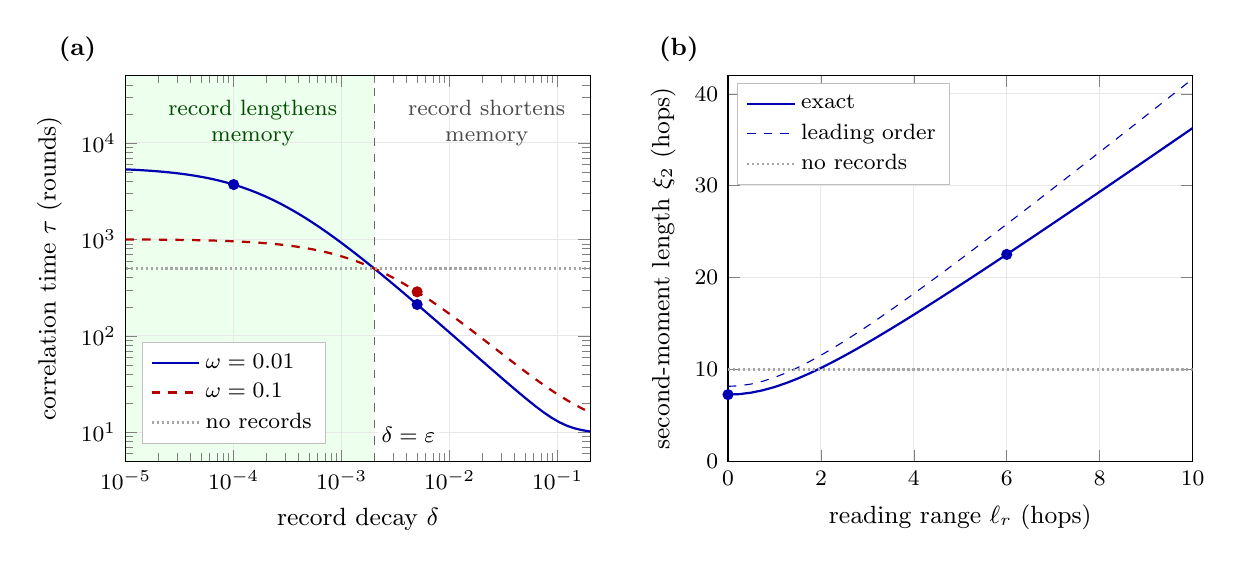
\begin{tikzpicture}
  \begin{loglogaxis}[name=pa, scale only axis, width=5.9cm, height=4.9cm, set layers,
      xmin=1e-5, xmax=0.2, ymin=5, ymax=5e4,
      xlabel={record decay $\delta$}, ylabel={correlation time $\tau$ (rounds)},
      grid=major, grid style={gray!18},
      legend style={font=\footnotesize, at={(0.035,0.045)}, anchor=south west, draw=gray!50, fill=white, cells={anchor=west}},
      every axis label/.style={font=\small}, tick label style={font=\footnotesize}]
    \begin{pgfonlayer}{axis background}
      \fill[green!7] (axis cs:1e-5,5) rectangle (axis cs:0.002,5e4);
    \end{pgfonlayer}
    % beta=0.1, omega=0.01 (R=10)
    \addplot[blue!70!black, thick] coordinates {(1e-05,5319.3) (1.1795e-05,5273.4) (1.3911e-05,5220.2) (1.6408e-05,5158.9) (1.9352e-05,5088.4) (2.2825e-05,5007.7) (2.6922e-05,4915.7) (3.1753e-05,4811.4) (3.7452e-05,4694) (4.4173e-05,4562.7) (5.21e-05,4417) (6.145e-05,4256.7) (7.2478e-05,4081.9) (8.5485e-05,3893.3) (0.00010083,3692.2) (0.00011892,3480.1) (0.00014026,3259.3) (0.00016543,3032.4) (0.00019512,2802.3) (0.00023014,2572.1) (0.00027144,2344.9) (0.00032016,2123.7) (0.00037761,1911) (0.00044538,1709.2) (0.00052531,1519.8) (0.00061958,1344.2) (0.00073077,1183) (0.00086191,1036.4) (0.0010166,904.25) (0.001199,786.05) (0.0014142,681.07) (0.001668,588.39) (0.0019674,507.03) (0.0023204,435.95) (0.0027368,374.11) (0.003228,320.5) (0.0038073,274.19) (0.0044906,234.27) (0.0052965,199.96) (0.006247,170.53) (0.0073681,145.32) (0.0086903,123.77) (0.01025,105.37) (0.012089,89.674) (0.014259,76.301) (0.016818,64.919) (0.019836,55.24) (0.023396,47.019) (0.027595,40.043) (0.032547,34.133) (0.038388,29.137) (0.045277,24.928) (0.053402,21.4) (0.062986,18.47) (0.074289,16.077) (0.087622,14.176) (0.10335,12.731) (0.12189,11.693) (0.14377,10.984) (0.16957,10.512) (0.2,10.196)};
    \addlegendentry{$\omega=0.01$}
    % beta=0.1, omega=0.1 (R=1)
    \addplot[red!70!black, thick, dashed] coordinates {(1e-05,999.45) (1.1795e-05,998.54) (1.3911e-05,997.48) (1.6408e-05,996.22) (1.9352e-05,994.75) (2.2825e-05,993.02) (2.6922e-05,990.98) (3.1753e-05,988.59) (3.7452e-05,985.78) (4.4173e-05,982.49) (5.21e-05,978.64) (6.145e-05,974.13) (7.2478e-05,968.87) (8.5485e-05,962.74) (0.00010083,955.61) (0.00011892,947.33) (0.00014026,937.76) (0.00016543,926.7) (0.00019512,914) (0.00023014,899.46) (0.00027144,882.9) (0.00032016,864.14) (0.00037761,843.01) (0.00044538,819.4) (0.00052531,793.19) (0.00061958,764.37) (0.00073077,732.98) (0.00086191,699.12) (0.0010166,663.03) (0.001199,625) (0.0014142,585.43) (0.001668,544.8) (0.0019674,503.61) (0.0023204,462.45) (0.0027368,421.84) (0.003228,382.33) (0.0038073,344.38) (0.0044906,308.38) (0.0052965,274.63) (0.006247,243.35) (0.0073681,214.65) (0.0086903,188.56) (0.01025,165.06) (0.012089,144.06) (0.014259,125.42) (0.016818,108.97) (0.019836,94.545) (0.023396,81.957) (0.027595,71.021) (0.032547,61.558) (0.038388,53.4) (0.045277,46.394) (0.053402,40.396) (0.062986,35.279) (0.074289,30.931) (0.087622,27.25) (0.10335,24.147) (0.12189,21.544) (0.14377,19.373) (0.16957,17.57) (0.2,16.083)};
    \addlegendentry{$\omega=0.1$}
    \addplot[gray!70, densely dotted, thick, domain=1e-5:0.2, samples=2] {499.4998};
    \addlegendentry{no records}
    \draw[black!60, dashed] (axis cs:0.002,5) -- (axis cs:0.002,5e4);
    \node[font=\footnotesize, anchor=south west, inner sep=1.5pt, fill=white, xshift=1pt] at (axis cs:0.002,7) {$\delta=\varepsilon$};
    % configurations of chk:sca-records-length (tau does not depend on the reading range)
    \addplot[only marks, mark=*, mark size=1.8pt, blue!70!black] coordinates {(1e-4,3702.5) (5e-3,211.3)};
    \addplot[only marks, mark=*, mark size=1.8pt, red!70!black] coordinates {(5e-3,286.1)};
    \node[font=\footnotesize, align=center, green!30!black] at (axis cs:1.5e-4,1.6e4) {record lengthens\\memory};
    \node[font=\footnotesize, align=center, black!70] at (axis cs:0.022,1.6e4) {record shortens\\memory};
  \end{loglogaxis}
  \node[font=\small\bfseries, anchor=south east] at ($(pa.north west)+(-0.25cm,0.05cm)$) {(a)};
  \begin{axis}[name=pb, at={($(pa.south east)+(1.75cm,0)$)}, anchor=south west, scale only axis, width=5.9cm, height=4.9cm,
      xmin=0, xmax=10, ymin=0, ymax=42,
      xlabel={reading range $\ell_r$ (hops)}, ylabel={second-moment length $\xi_2$ (hops)},
      grid=major, grid style={gray!18},
      legend style={font=\footnotesize, at={(0.02,0.98)}, anchor=north west, draw=gray!50, fill=white, cells={anchor=west}},
      every axis label/.style={font=\small}, tick label style={font=\footnotesize}]
    % exact, prop:sca-records-length(a)
    \addplot[blue!70!black, thick] coordinates {(0,7.2652) (0.25,7.3193) (0.5,7.4793) (0.75,7.7386) (1,8.0878) (1.25,8.5156) (1.5,9.011) (1.75,9.5635) (2,10.164) (2.25,10.804) (2.5,11.477) (2.75,12.178) (3,12.901) (3.25,13.645) (3.5,14.405) (3.75,15.178) (4,15.964) (4.25,16.76) (4.5,17.565) (4.75,18.378) (5,19.197) (5.25,20.022) (5.5,20.852) (5.75,21.687) (6,22.527) (6.25,23.369) (6.5,24.215) (6.75,25.064) (7,25.916) (7.25,26.77) (7.5,27.626) (7.75,28.484) (8,29.344) (8.25,30.206) (8.5,31.069) (8.75,31.933) (9,32.799) (9.25,33.666) (9.5,34.534) (9.75,35.403) (10,36.273)};
    \addlegendentry{exact}
    % leading order, eq:sca-records-xi
    \addplot[blue!70!black, dashed] coordinates {(0,8.165) (0.25,8.2285) (0.5,8.4163) (0.75,8.7202) (1,9.1287) (1.25,9.6285) (1.5,10.206) (1.75,10.849) (2,11.547) (2.25,12.29) (2.5,13.07) (2.75,13.882) (3,14.72) (3.25,15.579) (3.5,16.457) (3.75,17.351) (4,18.257) (4.25,19.176) (4.5,20.104) (4.75,21.041) (5,21.985) (5.25,22.936) (5.5,23.892) (5.75,24.854) (6,25.82) (6.25,26.79) (6.5,27.764) (6.75,28.741) (7,29.721) (7.25,30.704) (7.5,31.689) (7.75,32.676) (8,33.665) (8.25,34.656) (8.5,35.649) (8.75,36.643) (9,37.639) (9.25,38.636) (9.5,39.634) (9.75,40.633) (10,41.633)};
    \addlegendentry{leading order}
    \addplot[gray!70, densely dotted, thick, domain=0:10, samples=2] {9.995};
    \addlegendentry{no records}
    \addplot[only marks, mark=*, mark size=1.8pt, blue!70!black] coordinates {(0,7.265) (6,22.527)};
  \end{axis}
  \node[font=\small\bfseries, anchor=south east] at ($(pb.north west)+(-0.25cm,0.05cm)$) {(b)};
\end{tikzpicture}

  \caption{\textbf{Records on the ring.} Memory and reach of the agents on a ring with $a=0.2$ and $\varepsilon=0.002$, with one record per site, reading that displaces self-weight ($\upsilon=0$) and noiseless records ($q_z=0$). (a) The correlation time $\tau=-1/\ln(1-\varepsilon_{\mathrm{rec}})$, with $\varepsilon_{\mathrm{rec}}$ the root of \eqref{eq:sca-secular}, against the decay $\delta$ of a local record ($\ell_r=0$) with read weight $\beta=0.1$ and write weight $\omega=0.01$ or $0.1$. Both curves cross the value without records, $499.5$ rounds, at $\delta=\varepsilon$, as the exact criterion \eqref{eq:sca-memory-criterion} requires: in the shaded range $\delta<\varepsilon$ the record lengthens memory, and beyond it the record shortens memory. (b) The second-moment length $\xi_2$ of \cref{prop:sca-records-length}(a) against the reading range $\ell_r$ for the durable record $(\beta,\omega,\delta)=(0.1,0.01,10^{-4})$, whose correlation time is $3702.5$ rounds at every range. The dashed curve is $\bigl((a+\beta\ell_r^2/2)/(\varepsilon+\mathcal R\delta)\bigr)^{1/2}$, the limiting form in \eqref{eq:sca-records-xi}, which \cref{prop:sca-records-length}(b) proves to be the leading term as all leaks vanish; at these finite leaks the exact length lies below it. Read locally, the record slows the collective without widening it ($\xi_2=7.265$ hops, against $9.995$ without records); read at range, it widens it. Dots mark configurations of \cref{chk:sca-records-length}; $\tau$ does not depend on $\ell_r$.}
  \label{fig:sca-records}
\end{figure}

A record read by all members with a uniform kernel couples only to the mean mode: it acts on every deviation from the collective mean as an extra leak $\beta$, and it adds to every covariance a component that does not decay with distance and falls as $1/N$ (Supplement, \cref{rem:sca-global-records}).

\subsection{Long-range links}\label{sec:sca-longrange}

Media such as the telephone add links of every length. Let agents occupy $\Z^D$ with $W_{ij}=c\one\{i=j\}+a\mathsf J(x_i-x_j)$, where $c\ge0$, $a>0$, $\lambda=c+a<1$, and the link kernel $\mathsf J$ is a symmetric probability on $\Z^D\setminus\{0\}$ with a power-law tail $\mathsf J(x)\sim\mathsf J_\infty|x|^{-D-\sigma}$, $\sigma>0$; let $Q^\zeta=qI$. The density of link lengths decays as $l^{-1-\sigma}$, so its mean is finite exactly when $\sigma>1$.

\begin{proposition}[Algebraic decay]\label{prop:sca-longrange}
In this setting $\Sigma(x)/\mathsf J(x)\to2q\lambda a/(1-\lambda^2)^2$ as $|x|\to\infty$, which is $\simeq qa/(2\varepsilon^2)$ for small $\varepsilon=1-\lambda$. No exponential clustering holds, whatever $\varepsilon$. If the agents are not translation invariant but $\Vert W_{ij}\Vert\le c\one\{i=j\}+a\mathsf J(x_i-x_j)$ and the local noise blocks are $\preceq qI$, then $\limsup\Vert\Sigma_{ij}\Vert/\mathsf J(x_i-x_j)\le2q\lambda a/(1-\lambda^2)^2$ as $|x_i-x_j|\to\infty$.
\end{proposition}
% src: L4-P13 (limit; the correction order is heuristic and omitted)
Proof in \cref{app:sca}; checked on a ring of $2^{17}$ sites (\cref{chk:sca-longrange}). Two distant agents are correlated mostly through the single long link that joins them.

Under the hypotheses stated there, the front of the normalized influence grows like $t^{1/\min(\sigma,2)}$ for $\sigma\neq2$, so influence moves at finite speed if and only if $\sigma\ge1$ (Supplement, \cref{prop:sca-fronts}).

\subsection{Percolation of coherent information}\label{sec:sca-percolation}

Correlation is a second-order notion. Information about a source can reach farther than correlations suggest when receivers aggregate many paths, and less far when channels are nonlinear and noisy. We bound it on the space-time network of a protocol run.

\begin{definition}[Space-time network]\label{def:sca-spacetime}
A protocol run is a Bayesian network on a directed acyclic graph whose vertices are the agent states $X_{i,t}$, the messages $Y_{j\to i,t}$, outputs of channels applied to $X_{j,t}$, and the memory traces $\tilde X_{i,t}$, outputs of a forgetting channel applied to $X_{i,t}$, with $X_{i,t+1}=f_{i,t}(\tilde X_{i,t},(Y_{j\to i,t})_j,\zeta_{i,t})$ and fresh independent randomness $\zeta_{i,t}$. A source $X_{\mathrm{src}}$ enters only through $X_{0,0}$. For a channel $P_{Y\mid X}$, its strong data-processing coefficient is $s_{\mathrm{KL}}(P_{Y\mid X})=\sup I(X';Y)/I(X';X)$, the supremum running over laws of $X$ and over variables $X'$ with $X'\to X\to Y$. In site percolation each vertex is open independently with probability $s_{\mathrm{KL}}$ of the channel that produces it (one for agent states), and $\perc(X_{0,0}\to\mathcal S)$ is the probability of an open directed path from $X_{0,0}$ to the vertex set $\mathcal S$.
\end{definition}
% src: L4-D7; the source is written X_src because Upsilon_ij is the mistranslation of def:fw-translation

\begin{theorem}[Information percolation for message passing]\label{thm:sca-percolation}
If message channels have strong data-processing coefficient at most $s_e$ and memory channels at most $s_m$, then for every vertex set $\mathcal S$,
\begin{equation}\label{eq:sca-perc}
I(X_{\mathrm{src}};X_{\mathcal S})\le\perc(X_{0,0}\to\mathcal S)\cdot I(X_{\mathrm{src}};X_{0,0}).
\end{equation}
With maximal degree $\Delta$ and $d=d(0,i)$, $\perc(X_{0,0}\to X_{i,t})\le\sum_{k\ge d}\binom tk(\Delta s_e)^ks_m^{t-k}$, and when $s_m+\Delta s_e<1$,
\begin{equation}\label{eq:sca-perc-union}
\perc\bigl(X_{0,0}\to\{X_{i,t}\}_{t\ge0}\bigr)\le\frac{1}{1-s_m-\Delta s_e}\Bigl(\frac{\Delta s_e}{1-s_m}\Bigr)^d.
\end{equation}
Information about a one-shot source then decays exponentially in hop distance, uniformly in time, with information length $\xi_I=1/\ln((1-s_m)/(\Delta s_e))$.
\end{theorem}
% src: L4-P15 (application of Polyanskiy-Wu 2017, Theorem 5 and Corollary 7, read in primary text)
Proof in \cref{app:sca}, from Theorem~5 and Corollary~7 of \citet{polyanskiy2017strong}. For Gaussian channels without input constraints $s_{\mathrm{KL}}=1$, so the theorem is vacuous in the linear-Gaussian model, which the Gaussian results of the Supplement (\cref{thm:sca-trees,thm:sca-gaussian-percolation}) treat; with perfect memory ($s_m=1$) the bound grows with $t$, as it must for repeated transmissions of one content. For conventions checked pairwise through agreement observations that flip with probability $\delta_0$, the information that all observations and the conventions of a set $\mathcal S$ carry about one agent's convention is at most $\perc_{\mathcal G}(i,\mathcal S)\ln2$ in bond percolation with edge probability $(1-2\delta_0)^2$ \citep[Theorem~1]{polyanskiy2019application}, exponentially small in $d(i,\mathcal S)$ below the critical point on transitive graphs \citep{duminilcopin2016new} and whenever $(\Delta-1)(1-2\delta_0)^2<1$; group-wide consistency of conventions (\cref{sec:coh}) cannot be inferred beyond that scale.

In the linear-Gaussian model the decisive structure is branching. On the $b$-ary tree with edge correlation $\alpha$ and exactly observed leaves, the information that a level carries about the root stays bounded away from zero as the level recedes if and only if $b\alpha^2>1$; on a general locally finite tree with constant $\alpha$ and exact leaves it does so when the branching number $\mathrm{br}(T)$ satisfies $\mathrm{br}(T)\alpha^2>1$ and does not when $\mathrm{br}(T)\alpha^2<1$; and the information about a source upstream of the root obeys a percolation bound with edge probabilities $\alpha_e^2$ (Supplement, \cref{thm:sca-trees,thm:sca-gaussian-percolation}). On graphs whose spheres grow subexponentially, by contrast, aggregate information has short reach under the hypotheses stated there. The precision of the Gaussian law on the $b$-ary tree of depth at least two is not diffusive in plain coordinates when $b\alpha^2>1$, and a homogeneous diffusive medium on a regular tree of degree at least three admits no reconstruction, so a broadcast hierarchy can spread shared content without forming a collective in the sense of \cref{def:col-collective} (Supplement, \cref{prop:sca-aggregate,prop:sca-tree-diffusive}). That information about a common source reaches arbitrary hop distance when the effective branching number times $\alpha^2$ exceeds one, and is confined when it is below one, is a conjecture beyond trees (Supplement, \cref{conj:sca-condensation}).

\subsection{Coherence volume and the size of collectives}\label{sec:sca-volume}

The second-moment length bounds the extent of a contrast-selected collective (\cref{cor:col-lstar}). A different question is how many agents can be correlated at a given level with one collective variable, which we answer for linear readouts.

\begin{definition}[Correlational coherence of a set of agents]\label{def:sca-coherence}
For a set $C$ of agents with scalar readouts $X_i=\mathbf v_i^\top\mu_i/\sigma_i$, with unit vectors $\mathbf v_i$ and $\sigma_i$ the world-conditional standard deviation of $\mathbf v_i^\top\mu_i$, let $\mathrm{Corr}_C$ be their world-conditional correlation matrix. The correlational coherence of $C$ with a variable $Z$ is $\theta_Z(C)=\min_{i\in C}\Corr(X_i,Z)$, its best correlational coherence is $\theta^\ast(C)=\sup_Z\theta_Z(C)$, and its susceptibility is $\chi_C=\max_{i\in C}\sum_{j\in C}|(\mathrm{Corr}_C)_{ij}|$. For $\theta>0$, a set of agents is $\theta$-coherent with $Z$ when each of its members has $\Corr(X_i,Z)\ge\theta$. This is a statement about correlation with a variable and is distinct from the coherence score of \cref{def:coh-components}, which pairs a fidelity, calibration or consistency quantity of the communication inside the set with the inaccuracy of its members. In \cref{sec:sca-volume}, coherence without a qualifier and the coherence count refer to correlational coherence.
\end{definition}
% src: L4-D6

\begin{theorem}[Coherence volume]\label{thm:sca-coherence-volume}
Let $\mathbb P_C$ be the set of probability vectors on $C$.
\begin{enumerate}
\item[(a)] $\theta^\ast(C)>0$ exactly when $\min_{p\in\mathbb P_C}p^\top\mathrm{Corr}_Cp>0$. In that case $\theta^\ast(C)$ is attained by a variable in the linear span of the readouts and $\theta^\ast(C)^2=\min_{p\in\mathbb P_C}p^\top\mathrm{Corr}_Cp$, the variance of the minimum-variance convex combination of the members; the optimal collective variable is proportional to $p^{\ast\top}X$. Otherwise some convex combination of the readouts vanishes, no variable is positively correlated with every member, and $\theta^\ast(C)=0$, attained by any variable uncorrelated with the readouts, which need not lie in their span: for $X_2=-X_1$ every nonzero element of the span has minimum correlation $-1$.
\item[(b)] $\theta^\ast(C)^2\le\one^\top\mathrm{Corr}_C\one/|C|^2\le\lambda_{\max}(\mathrm{Corr}_C)/|C|\le\chi_C/|C|$.
\item[(c)] For any variable $Z$ and $\theta>0$, at most $\chi_C/\theta^2$ members of $C$ have $\Corr(X_i,Z)\ge\theta$.
\item[(d)] If the unit top eigenvector $\mathbf w$ of $\mathrm{Corr}_C$ is positive, $\theta^\ast(C)\ge\lambda_{\max}(\mathrm{Corr}_C)^{1/2}\min_iw_i$, so (b) is attained up to the delocalization of $\mathbf w$.
\end{enumerate}
\end{theorem}
% src: L4-T4
Proof in \cref{app:sca}; checked on disks in the two-dimensional medium (\cref{chk:sca-coherence-volume}). A collective much larger than its susceptibility has no coherent interior, and the susceptibility is bounded by the contraction.

\begin{corollary}[Size of coherent collectives]\label{cor:sca-size}
Assume \textup{(M)}, \textup{(Lin)}, \textup{(Loc)} and \textup{(B)}.
\begin{enumerate}
\item[(a)] Under \textup{(C$_{rc}$)}, $\chi_C\le q/(q_{\min}(1-\lambda_r\lambda_c))$, so $|C|\theta^\ast(C)^2\le q/(q_{\min}(1-\lambda_r\lambda_c))$ for every $C$.
\item[(b)] Under \textup{(C$_\rho$)}, $|C|\theta^\ast(C)^2\le\lambda_{\max}(\mathrm{Corr}_C)\le K_A^2q/(q_{\min}(1-f^2))$, which is $K_A^2q\tau_f/(2q_{\min})(1+O(1-f))$ with $\tau_f=-1/\ln f\ge\tau$.
\item[(c)] On the complete graph with $W_{ij}=\lambda/N$ for all $i,j$ and $Q^\zeta=qI$, $N\theta^\ast(V)^2=\lambda_{\max}(\mathrm{Corr}_V)=1/((1-\lambda^2)(1+b_N))$ with $b_N=\lambda^2/((1-\lambda^2)N)$, which tends to the bound $1/(1-\lambda^2)$ of (a) and (b) as $N\to\infty$.
\item[(d)] In the medium of \cref{thm:sca-oz} with $c>0$, $\chi=q/((1-\lambda^2)\Sigma(0))$. As $\varepsilon\to0$ this gives $\chi\simeq2\xi_{\mathrm{OZ}}$ for $D=1$, $\chi\simeq4\pi a/(\varepsilon\ln(1/\varepsilon))$ for $D=2$, and $\chi\simeq q\xi_2^2/(2a\Sigma(0))\propto\xi_2^2$ for $D\ge3$. A $\theta$-coherent set of agents therefore has at most of order $2\xi/\theta^2$ members in one dimension, $\xi^2/(\theta^2\ln\xi)$ in two and $\xi^2/\theta^2$ in three or more.
\item[(e)] The bounds fail with neither \textup{(C$_{rc}$)} nor \textup{(C$_\rho$)} with constants uniform in the size of the network. If a hub that attends nobody ($W_{hh}=c_h$) is attended by $N$ leaves ($W_{\ell h}=a$, $W_{\ell\ell}=c$), every pair of leaves has the same positive correlation $\theta_\star$, independent of $N$, so for $\theta^2<\theta_\star$ arbitrarily many leaves are $\theta$-coherent with one variable; the hub's column sum $c_h+Na$ is unbounded in $N$, and so is every constant $K_A$ of \textup{(C$_\rho$)}, since $K_Af\ge\Vert W\Vert\ge(c_h^2+Na^2)^{1/2}$.
\end{enumerate}
\end{corollary}
% src: L4-P18 (with the C_rc hypothesis made explicit), B3-P2(b) (spectral form, V10 repair of the memory gloss)
Proof in \cref{app:sca}; checked on the complete graph (\cref{chk:sca-coherence-volume}). Part (b) is the precise form of the statement that volume is limited by memory, with the transient factor $K_A^2$; part (a) is not a memory statement, since $1/(1-\lambda_r\lambda_c)$ can be large when $\tau=0$, as in a directed copy chain. With $|C|\asymp L^D$, part (d) gives $L\lesssim2\xi/\theta^2$ for $D=1$, $L\lesssim\xi/(\theta\sqrt{\ln\xi})$ for $D=2$ and $L\lesssim(\xi/\theta)^{2/D}$ for $D\ge3$: H4's bound $L\lesssim\xi$ is right in low dimension and loose in high dimension, where correlations within $\xi$ already decay like $r^{-(D-2)}$. Part (e) is a formal counterpart of Deutsch's thesis that nations are defined by the reach of social communication \citep{deutsch1953nationalism}, a reading we offer as interpretation. Scale-free correlations in starling flocks \citep{cavagna2010scale} sit at or beyond the boundary $L\sim\xi$ of this linear theory; their mechanism, a broken continuous symmetry, lies outside the massive linear model. \Cref{tab:sca-sizes} relates the size notions of the manuscript to the largest extent $\Lstar$.

\begin{table}[t]
\centering
\small
\begin{tabular}{@{}>{\raggedright\arraybackslash}p{0.2\textwidth}>{\raggedright\arraybackslash}p{0.27\textwidth}>{\raggedright\arraybackslash}p{0.45\textwidth}@{}}
\toprule
Notion & Bound and hypotheses & Relation to $\Lstar$\\
\midrule
Largest extent $\Lstar$ (\cref{def:col-lstar}) & $\Lstar\le\xi_2/\sqrt{r_0-1}$ per coordinate (\cref{cor:col-lstar}); \textup{(M)}, diffusive precision, uniform leak & An upper bound only; $\Lstar=0$ in homogeneous media at every admissible level.\\
Coherence count (\cref{thm:sca-coherence-volume}) & $|C|\le\lambda_{\max}(\mathrm{Corr}_C)/\theta^2\le\chi_C/\theta^2$ for a $\theta$-coherent set; \textup{(M)}, with \textup{(C$_{rc}$)} to bound $\chi_C$ or \textup{(C$_\rho$)} to bound $\lambda_{\max}(\mathrm{Corr}_C)$ (\cref{cor:sca-size}) & Not comparable in general: contrast implies coherence for small regions (\cref{prop:col-coherence-average}), while a homogeneous medium has a large coherence count and $\Lstar=0$.\\
Information reach (\cref{thm:sca-trees}) & reconstruction if $\mathrm{br}(T)\alpha^2>1$, none if $\mathrm{br}(T)\alpha^2<1$; Gaussian broadcast & Not comparable: reach needs $b\alpha^2>1$, hence $b\alpha>1$, outside the diffusive class (\cref{prop:sca-tree-diffusive}).\\
One-round diameter (\cref{prop:abs-one-round}) & set by travel within one round & Composable, not comparable: the one-round reach bounds the hop length, and contrast bounds the extent in hops (\cref{cor:abs-one-round-extent}).\\
\bottomrule
\end{tabular}
\caption{Four size notions. Each answers a different question, so a bound on one is not a bound on another unless the table says so.}
\label{tab:sca-sizes}
\end{table}
% src: B1 comparability table (Section 4), critic D7

Scale also limits what is shared, since content that crosses many hops passes through many codes. For fixed noiseless codes read in a common prior metric, the content that survives an arbitrarily long relay is the common ground, the intersection of the subspaces that the codes transmit, approached geometrically when the hops recur in cyclic or quasi-periodic order (Supplement, \cref{sec:sca-abstraction,thm:sca-alternating}). That the effective rank of the content shared across $n$ hops tends generically to one in relay networks with diverse codes or frames, and does not increase with $n$ when the codes share a direction, is conjectured; for fixed noiseless codes in a common metric that share no direction it can rise from one hop to the next (Supplement, \cref{conj:sca-rank-down,ex:ren-rank-nonmonotone}).

\subsection{Hypothesis H4 in final form}\label{sec:sca-h4}

We collect what is proved. The theorem restates results of this section and of \cref{sec:col}; each part names its hypotheses.

\begin{theorem}[Hypothesis H4, final form]\label{thm:sca-h4}
Let the agents' world-conditional errors follow \eqref{eq:sca-recursion} under \cref{asm:sca-standing}, with \textup{(Loc)} and \textup{(B)}.
\begin{enumerate}
\item[(a)] Without the moment bound. For every local rule and every start that is world-conditionally independent across agents and independent of the noises, agents farther apart than $2t$ hops are world-conditionally independent after $t$ rounds. Under \textup{(Lin)}, with initial errors independent across agents and block covariances at most $q_0I$, correlations of level $\theta$ reach at most $\min\{2t,2v_\varphi t+\varphi^{-1}\ln(K_\varphi/\theta)\}$ hops at time $t$, for every $\varphi>0$ with $g_\varphi>1$, where $K_\varphi=(q/(g_\varphi^2-1)+q_0)/q_{\min}$ as in \cref{thm:sca-no-moment}(b). When \textup{(M)} fails in both its stationary and its uniform form there is no correlation length in the sense of \cref{def:sca-lengths}; when the stationary form fails there is no stationary law with finite second moments and, by \cref{def:col-collective}, no collective.
\item[(b)] Correlation length. Assume \textup{(M)} and \textup{(Lin)}. Then $\xi\le1/\ln(1/\lambda)$ under \textup{(C$_r$)}; $\xi\le\tau$ under \textup{(C$_\rho$)}; and $\xi\le1/\sqrt{2\ln(1/\lambda)}$ when $W(t)$ is dominated by $\lambda$ times a reversible chain whose measure has bounded ratio $\varpi_{\max}/\varpi_{\min}$. Under \textup{(TI)} on $\Z^D$ with $W_{ii}=c\ge0$, $W_{ij}=a$ between nearest neighbors and $Q^\zeta=qI$, the Ornstein--Zernike length in each coordinate direction is exactly $\xi_{\mathrm{OZ}}=1/\arccosh(1+\varepsilon/(2a))$ with $\varepsilon=1-c-2Da$, the second-moment length is $\xi_2=(2a\lambda/(1-\lambda^2))^{1/2}\le\min\{\xi_{\mathrm{OZ}},(a/\varepsilon)^{1/2}\}$, and $\xi_{\mathrm{OZ}}=(a/\varepsilon)^{1/2}(1+O(\varepsilon))$. Physical lengths are these times the hop length $\ell$.
\item[(c)] Communication range. For a translation-invariant diffusive world-conditional precision with leak $\varepsilon^\Pi>0$ and couplings of finite range $\ell^\Pi_d$ in direction $d$ with $\varsigma_d>0$, $\xi_{2,d}\le\xi_{\mathrm{OZ},d}\le\xi_{2,d}(\cosh(\ell^\Pi_d/\xi_{2,d}))^{1/2}$, and $\xi_{2,d}^2=\varsigma_d^2/(2\varepsilon^\Pi)$ grows with the second moment of the couplings. For attention weights with power-law tails $\mathsf J(x)\sim\mathsf J_\infty|x|^{-D-\sigma}$ in the setting of \cref{prop:sca-longrange}, where $W_{ij}=c\one\{i=j\}+a\mathsf J(x_i-x_j)$, $\lambda=c+a<1$ and $Q^\zeta=qI$, no exponential clustering holds, $\Sigma(x)/\mathsf J(x)\to2qa\lambda/(1-\lambda^2)^2$, and influence moves at finite speed if and only if $\sigma\ge1$.
\item[(d)] Correlation time and records. Under \textup{(M)} and \textup{(Lin)} with $W$ and $Q^\zeta\succ0$ time invariant, a linear collective variable keeps correlation $\theta$ for at most $T^\ast(\theta)\le\ln(1/\theta)/\ln(1/\Vert\tilde W\Vert)$ rounds, and $T^\ast(\theta)\sim\tau\ln(1/\theta)$ as $\theta\to0$. In the medium of (b), $\xi_2^2/\tau\to a$ as $\varepsilon\to0$. In the record model with $I-\mathsf R\ge0$ the correlation time of the mean mode is $-1/\ln(1-\varepsilon_{\mathrm{rec}})$, with $\varepsilon_{\mathrm{rec}}$ the root of the secular equation. With reading that displaces self-weight, records lengthen it if and only if $\sum_k\beta_k(\delta_k-\varepsilon)/(\omega_k+\delta_k-\varepsilon)<0$ (when $\varepsilon<\min_k(\omega_k+\delta_k)$), and as all leaks vanish $\tau=(1+o(1))(1+\sum_k\mathcal R_k)/(\varepsilon+\sum_k\mathcal R_k\delta_k)$ and, for $a>0$, $\xi_2^2=(1+o(1))(a+\sum_k\beta_k\ell_{r,k}^2/2)/(\varepsilon+\sum_k\mathcal R_k\delta_k)$.
\item[(e)] Extent. Under \textup{(M)} and a diffusive world-conditional precision with uniform leak, every region with contrast at least $r_0>1$ has root-mean-square extent at most $\xi_{2,d}/\sqrt{r_0-1}$ in each coordinate, so $\Lstar\le\xi_2/\sqrt{r_0-1}$. In the record model the same holds for regions of agents with the length of \cref{prop:sca-records-length}(a), provided the world-conditional precision of agents and records is diffusive. The number of members that are $\theta$-coherent with any one variable is at most $\chi_C/\theta^2$, where, under \textup{(M)} and \textup{(Lin)}, $\chi_C\le q/(q_{\min}(1-\lambda_r\lambda_c))$ under \textup{(C$_{rc}$)} and $|C|\theta^\ast(C)^2\le K_A^2q/(q_{\min}(1-f^2))$ under \textup{(C$_\rho$)}; with neither \textup{(C$_{rc}$)} nor \textup{(C$_\rho$)} with constants uniform in the size of the network, a broadcaster makes the number unbounded.
\end{enumerate}
\end{theorem}
% src: assembled from thm:sca-lightcone, thm:sca-no-moment, thm:sca-clustering, prop:sca-spectral, thm:sca-diffusive, thm:sca-oz, prop:sca-lengths-relation, prop:sca-longrange, prop:sca-fronts, prop:sca-persistence, prop:sca-diffusive-scaling, prop:sca-records, prop:sca-records-memory, prop:sca-records-length, thm:sca-coherence-volume, cor:sca-size; thm:col-contrast-size, cor:col-lstar; M_spec decisions 3, 13, 16
Proof in \cref{app:sca}. In words, the correlation length grows like $\ell\sqrt{a/\varepsilon}$, and like the square root of the couplings' second moment when links are longer; the correlation time $\tau=-1/\ln\rho$ of agents and media together, with $\rho$ the spectral radius of their joint transition matrix, which is the inverse spectral gap to leading order as $\rho\to1$, is lengthened by records exactly under the criterion of (d); and the extent of a collective is at most $\xi_2/\sqrt{r_0-1}$. Apart from the exact lengths of (b) and (c), namely the Ornstein--Zernike length of nearest-neighbor passing and the second-moment lengths, and the exact secular root and memory criterion of the record model, these are upper bounds for linear, local, bounded networks, \textup{(Lin)}, \textup{(Loc)} and \textup{(B)}, conditional on \textup{(M)} and a named contraction, and none says that collectives of that size form. Under coarse-graining the axis rate and the second-moment length of (b) and (c) have exact flows, with the leak relevant and time rescaled by the square of the block factor (\cref{thm:ren-flows,prop:ren-exponents}), and the size bound of (e), applied level by level, limits the depth of a hierarchy of collectives (\cref{prop:ren-depth}); which parameters of the framework survive coarse-graining, exactly or up to an error set by the dispersion of the cut against the stiffnesses $\xin$ and $\xout$ of the blocks, which high contrast alone does not make small, is the subject of \cref{thm:ren-closure}.

Several things are not established. The exact pointwise rates and the Ornstein--Zernike prefactor in dimension two and higher rest on a restated theorem and a heuristic step (\cref{rem:sca-oz-form}). The size bound with records needs a diffusive precision of agents and records, which fails with record noise in a computed case, and contrast is not defined for the non-diffusive precisions that non-reciprocal attention produces (\cref{open:col-non-diffusive}). Condensation beyond trees (\cref{conj:sca-condensation}), the decline of shared rank with scale, which need not be monotone along relays whose codes share no direction (Supplement, \cref{conj:sca-rank-down,ex:ren-rank-nonmonotone}), and the absence of amplification with one code (\cref{conj:sca-common-code}) are conjectures. Finally, the theorem treats $a$ and $\varepsilon$ as given.

Whether attention selected by expected free energy, together with grounding, drives $a$ and $\varepsilon$ toward the regime in which the largest extent $\Lstar$ of collectives is comparable to $\xi_2$ is an open problem (Supplement, \cref{open:sca-endogenous}).

\section{The minimal model revisited}\label{sec:min}
% src: L7 Sections 1 to 3, 5 and 6; answers to L7-E7, L7-E11, L7-E12, L7-O5 in the change lists of B4 and B5; dennis2026communicating

The research report of November 7, 2026 \citep{dennis2026communicating} studied a minimal version of the present framework: a linear-Gaussian world, agents that sense blocks of it, rank-limited messages in private linear encodings, attention and transmission chosen by expected free energy, and receivers that read messages as noisy observations of the world. It asked whether such agents condense into interior agents surrounded by a Markov blanket of agents, the picture behind hypothesis H1, and it obstructed that hypothesis without refuting it: message-fed blankets of agents exist as strict, locally stable orbits in four declared variants of the model, and none both passes the report's attribution rule and is reached from an uninformed start more often than under a null that randomizes partners. Its results are derivations, exhaustive enumerations and searches at declared parameter points, and mean-field computations; it simulated no sample path. This section states two results about the moment bound, one for a common rank-one code and one for noiseless grounding. The Supplement (\cref{sup:min}) places the earlier model inside the framework, sorts its results by how much they use the private encodings, restates the main ones with their scope, proves a third result about the moment bound, on its failure, and says which conclusions the framework's additions reopen and where they are now answered. Numbers quoted from the report are its own; \cref{chk:min} reproduces those on which this section relies.

The earlier model is the linear-Gaussian case of the agent model of \cref{def:fw-system} with an exogenous world, one round per world step, linear encodings and a single modality in every computed instance. The Supplement gives the dictionary between the two models and sorts the report's results into classes by how much of the encoding structure they use (\cref{sec:min-dictionary,def:min-classes}). It restates the report's message-fed bilayers, the four variants in which the report found them and the reasons none qualifies (\cref{sec:min-bilayers,def:min-bilayer}), and the report's attention structures, with a remark on why the reciprocal pairs of its replicator analysis need differences between frames (\cref{sec:min-attention,rem:min-reciprocity}).

\subsection{Double counting and the moment bound}\label{sec:min-moment}

Every length and time of the scale theory, and the definition of a collective, assume the moment bound (M): a stationary world-conditional law with finite second moments or, when attention changes from round to round, second moments bounded uniformly in time (\cref{asm:sca-standing,def:col-collective}); the report's version bounds the second moments of the decision-time belief means. The report found that its receivers' attention can violate it. This subsection states what restores the bound; the misreading behind that failure and the proof of when the failure starts are in the Supplement.

The misreading behind the failure is double counting: a level-1 receiver treats the error of a sender's posted predictive mean as independent of its own (Supplement, \cref{sup:min-double-counting-and-amplification}). The failure can start in a single round. When two agents that do not sense listen only to each other at level 1 with known rank-one codes, the reception step multiplies the homogeneous part of their disagreement by a matrix whose spectral radius exceeds one exactly under a criterion that proportional codes never meet (Supplement, \cref{lem:min-disagreement}, under the hypotheses stated there). Expected free energy selects a loop of mutual listening, in which both agents also sense, in the two-agent profile of the supplement (\cref{ex:sca-amplifying-profile}), whose frozen mean map has spectral radius $1.0613$ (\cref{chk:min-amplification}); this profile is the two-agent counterexample referred to below. It uses sender-specific codes, and one common code removes the amplification in two cases.

\begin{proposition}[One common rank-one code]\label{prop:min-common-code}
Let the effective codes be positive multiples of one nonzero row vector, $H_j=\vartheta_jT_c$ with $T_c\in\R^{1\times K}$ and $\vartheta_j>0$ (at identity encodings $\vartheta_j=1$), let the channel noise be $R_c=1$ (a sender-dependent noise variance can be absorbed into $\vartheta_j$), and let receivers know the codes and read at level 1. In one round let agent $i$ have decision-time covariance $P_i\succ0$ with precision $\Lambda_i=P_i^{-1}$, sensing information $\Gamma_i=(H^s_i)^\top(R^s_i)^{-1}H^s_i\succeq0$ (zero if it does not sense) and listening set $J_i$. Put $\alpha_j=\vartheta_j^2/(1+\vartheta_j^2T_cP_jT_c^\top)$ and $\Lambda^+_i=\Lambda_i+\Gamma_i+\sum_{j\in J_i}\alpha_jT_c^\top T_c$, and let $W^{\mathrm{rec}}$ be the homogeneous reception map
\begin{equation}\label{eq:min-reception}
e_i\mapsto(\Lambda^+_i)^{-1}\Bigl[\Lambda_ie_i+\sum_{j\in J_i}\alpha_jT_c^\top T_ce_j\Bigr],\qquad i\in V.
\end{equation}
\begin{enumerate}
\item[(a)] If listening is symmetric ($j\in J_i$ exactly when $i\in J_j$), then $W^{\mathrm{rec}}$ is self-adjoint for the inner product $\langle x,y\rangle_{\tilde M}=x^\top\tilde My$ with $\tilde M=\diag_i(\alpha_i\Lambda^+_i)$, it is diagonalizable with real spectrum in $(-1,1]$, and its eigenspace for the eigenvalue $1$ is
\[
\mathcal P=\bigl\{e:H^s_ie_i=0\text{ for every }i,\quad T_ce_i=T_ce_j\text{ whenever }j\in J_i\bigr\}.
\]
\item[(b)] If in addition the profile is frozen at a covariance fixed point and the world is isotropic, $F=fI_K$ with $0<f<1$, the error-transfer matrix $W=fW^{\mathrm{rec}}$, which is the matrix of \cref{def:fw-level0} with these level-1 gains, satisfies $\rho(W)\le f$ and $\Vert W^t\Vert_2\le K_{\tilde M}f^t$ for every $t\ge0$, with $K_{\tilde M}=(\lambda_{\max}(\tilde M)/\lambda_{\min}(\tilde M))^{1/2}$. Equality $\rho(W)=f$ holds exactly when $\mathcal P\neq\{0\}$, which is the case unless $\ker H^s_i\cap\ker T_c=\{0\}$ for every agent and every connected component of the listening graph contains an agent whose sensing map is injective. If channel noises are specific to each receiver, so that the local noise is independent across agents with blocks bounded by $q$, the world-conditional covariance satisfies
\[
\Vert\Sigma^c_{ij}\Vert\le\frac{K_{\tilde M}^2qf^{d(i,j)}}{1-f^2},
\]
with $d$ the hop distance on the listening graph.
\item[(c)] If no agent senses, then $\rho(W^{\mathrm{rec}})=1$ for every listening relation, symmetric or not, and every choice of the scales $\vartheta_j$. In the world $F=fI_K$, at a covariance fixed point of a frozen profile $\rho(W)=f=\rho(F)$, and along a periodic covariance orbit of a profile of period $p$ the map over one period has spectral radius $f^p$.
\end{enumerate}
\end{proposition}
% src: L7-P2, L7-P3 (a), (b), (b'), (c); B3-P1 row (ii) and B3-P2(a) for the spectral form; the periodic case of (c) and the characterization of P = {0} are added here
Proof in \cref{app:min}; the spectral statements were also checked numerically (\cref{chk:min-common-code}). The subspace $\mathcal P$ holds the error configurations that no agent's sensing sees and on which neighbors' coded messages agree, so no message can correct them: agreement in expression with disagreement in private opinion, as in discourse-sheaf models of opinion dynamics \citep{hansen2021opinion}, here an unobservable error mode. By part (b), with one code a community relaxes faster than the world only if every member senses all directions but at most one, which the code must read, and some member of each listening component senses every direction. Part (c) proves, for one common rank-one code in an isotropic world, the report's conjecture that a frozen profile in which no agent senses has a mean map of spectral radius below one, with the value $f$: a pure-listening community relaxes only at the world's own rate, whether its attention is frozen or switches periodically. The clustering bound of part (b) holds where the row-sum contraction of the clustering theorem fails in most instances (377 of 400 in \cref{chk:min-common-code}), which is why the scale theory needs its spectral form (\cref{prop:sca-spectral}).

Parts (b) and (c) prove two cases of \cref{conj:sca-common-code}; the cases, the computations that support the conjecture and the return of sender-specific codes with several modalities are discussed in the Supplement (\cref{sup:min-double-counting-and-amplification}). Noisy sensing does not restore (M), since both agents of the two-agent counterexample sense every round. Noise-free observation of the world does, above a rate.

\begin{proposition}[Noiseless grounding restores the moment bound]\label{prop:min-grounding-moment}
Let $Q\succ0$, let receivers know the senders' effective codes $H_j$, of any rank, and read at level 1 with assigned noise $\hat R_{ij}=R_c+H_jP_jH_j^\top$, $R_c\succ0$, the channel noise being independent across senders and of the sensing noise. Let attention depend on the past in any way, with at most $\bar J$ receivers listening to any one sender in a round; let $\eta_0\sim\Ncal(0,P_0)$, let the initial errors have finite second moments and let $Q\preceq P_i(0)\preceq P_0$ for every $i$. Suppose that in each round each agent, independently of everything else and with probability $p_g$, observes $\eta_t$ without noise, so that its posterior error is zero. Put
\begin{gather*}
\varpi_Q=1-\frac{1}{\lambda_{\max}(Q^{-1}P_0)},\qquad\mathrm{snr}_j=\lambda_{\max}\bigl(R_c^{-1/2}H_jP_0H_j^\top R_c^{-1/2}\bigr),\\
\varpi_H=\max_j\frac{\mathrm{snr}_j}{1+\mathrm{snr}_j},\qquad\varpi_g=(1-p_g)\varpi_Q(1+\varpi_H\bar J).
\end{gather*}
Then $\mathcal V(t)=\sum_ie_i(t)^\top\Lambda_i(t)e_i(t)$ satisfies $\E\mathcal V(t+1)\le\varpi_g\E\mathcal V(t)+N\tr(P_0)/\lambda_{\min}(Q)$, and the part of the error recursion that does not involve new noise contracts $\mathcal V$ in mean by the factor $\varpi_g$. If $\varpi_g<1$, the second moments of the errors and of the decision-time belief means are bounded uniformly in time, which is (M) in its uniform form.
\end{proposition}
% src: L7-P4 (the report's projection, header and prediction-contraction lemmas are reproved in the appendix); B3-P1 row (vi)
Proof in \cref{app:min}. In the two-agent counterexample $\varpi_Q=0.81$, $\mathrm{snr}_j=9/0.19$, $\varpi_H=0.97933$ and $\bar J=1$, so grounding each agent with probability above $0.3763$ per round restores the bound (\cref{chk:min-grounding-moment}). At $p_g=0$ the proposition is a small-gain condition like the report's, except that the report bounds the largest weighted error and so carries the capacity $\kappa$, while the sum over agents carries the number $\bar J$ of listeners of one sender, and only the sum lets independent grounding help. The conclusion applies when attention changes from round to round; it gives neither pathwise contraction nor covariance clustering. The report's grounding rounds, which show a public referent unrelated to $\eta$ so that translations can be identified, carry no information about $\eta$ and do not restore (M); joint-attention grounding, a noisy observation of the attended part of $\eta$, lies between the two cases and is open.

The Supplement restates the report's group-agency results and the two formalizations of the preference to predict and be predicted, between which the framework leaves the choice open (\cref{sec:min-agency}). It also lists the conclusions of the report that grounding, records, performative acts and multiplexity may change and where they now stand: three are answered within a stated scope, eleven in part, and three remain open (\cref{sec:min-reexamination}). The calculation the report expected to change its verdict becomes a question about collectives, which is an open problem (\cref{open:min-exact-fusion}).

\section{Abstract collectives}\label{sec:abs}
% src: L5 (all); L7-P13; critic V12, D6, C5, C7; B5 Sections 3.3 and 4 (B5-D3, B5-L2, B5-P12); B1-P7; B4 Section 1.5; decision 12

Cultures, economies, nations and cities are treated here as candidate collectives whose members are joined by conventions, exchange, law and co-presence rather than by one physical medium; they are the abstract agents of \cref{sec:int}. The device for treating them is the multiplex of \cref{asm:int-a9}: one population that communicates through several modalities, each with its own content, code, range, message weight, leak and memory. The main text states the results on multiplex populations, barriers, prices, polity size and scale-free coherence; records and media, cultures, cities and the comparison of world-conditional with unconditional correlations are treated in the Supplement (\cref{sup:abs}).

Propositions are exact statements about stated models, and conjectures need further proof or data. Every reading of a social-science finding is an interpretation or a conjecture, in a labeled remark or in prose marked as our reading, and claims no more about a cited work than the level at which we read it. The dynamic models are linear and Gaussian with a stable update, so the moment bound (M) of \cref{asm:sca-standing} holds, and each dynamic proposition names its contraction in the labels of \cref{sec:sca}. Contrast (\cref{def:col-contrast}) is defined only for diffusive world-conditional precisions, and most statements here use instead the ultrametric diagnostic of \cref{def:col-ultrametric}, with weights $\varpi_{ij}=-\ln\Gamma_{ij}$, ultrametric $u(i,j)$, heights $u_{\mathrm{in}}(C)$ and $\varpi_{\mathrm{out}}(C)$ and contrast $\mathcal U(C)=\varpi_{\mathrm{out}}(C)-u_{\mathrm{in}}(C)$, computed from world-conditional correlations unless we say otherwise and related to spectral contrast only within the scope of \cref{thm:col-bridge}.

\subsection{Multiplex populations}\label{sec:abs-multiplex}

A society communicates through language, exchange, law and co-presence at once; the first question is when these modalities can be treated separately, each with its own correlation length.

\begin{definition}[Multiplex population]\label{def:abs-multiplex}
A multiplex population is a population of agents as in \cref{def:fw-system} in which every channel carries one modality $c\in\mathcal M$ (\cref{def:col-nested}) and whose world state splits into contents, $\eta=(\eta^{(c)})_{c\in\mathcal M}$. Modality $c$ has a content $\eta^{(c)}$; a code $T_c$ of rank $r_c$ that reads the sender's beliefs about $\eta^{(c)}$, with receivers whose message likelihood involves only $\eta^{(c)}$ (block-pure codes); an attention graph $\mathcal G_c$ with hop length $\ell_c$ and message weight $a_c$; a leak $\varepsilon_c$ made of grounding, forgetting and turnover with fresh priors; a medium, transient or a record (\cref{def:fw-record-model}); and a flag saying whether its messages are performative (\cref{prop:fw-performative}). Agent $i$'s error splits into blocks $e^{(c)}_i$, the errors of its beliefs about $\eta^{(c)}$.
\end{definition}
% src: L5-D1, L5-D2

\Cref{tab:abs-modalities} lists the four modalities of this section. The multilayer-network terminology and the budget-optimal attention of one agent to independently evolving contents (\cref{prop:env-multiplex}(d)) are in the Supplement (\cref{sup:abs-multiplex-terminology}).

\begin{table}[t]
\centering\small
\caption{The four modalities of abstract collectives.}
\label{tab:abs-modalities}
\begin{tabular}{@{}>{\raggedright\arraybackslash}p{0.14\textwidth}>{\raggedright\arraybackslash}p{0.19\textwidth}>{\raggedright\arraybackslash}p{0.19\textwidth}>{\raggedright\arraybackslash}p{0.21\textwidth}>{\raggedright\arraybackslash}p{0.13\textwidth}@{}}
\toprule
Modality & Content & Typical messages & Medium & Performative\\
\midrule
Language and convention & parameters of codes; expectations about others' policies & utterances, gestures, texts & speech (transient); writing and artifacts (records) & rarely\\
Exchange & holdings and values of goods; commitments & prices, offers, transfers, balances & quotes (transient); ledgers and money (records) & transfers\\
Law and enforcement & rules in force, rights, pending sanctions & statutes, rulings, registrations, sanctions & statutes and registries (records) & rulings, sanctions\\
Co-presence & locations and activities of people & encounters & none & sometimes\\
\bottomrule
\end{tabular}
\end{table}

\begin{proposition}[Decoupled modalities]\label{prop:abs-decoupling}
Assume that (a) the world evolves as $\eta_{t+1}=F\eta_t+w_t$, without performative acts, with $F$ and $Q$ block diagonal across contents; (b) every agent's initial posterior covariance is block diagonal, and the pairs $(e^{(c)}(0),\eta^{(c)}_0)$ of initial errors and world blocks are independent across contents; (c) codes and message likelihoods are block pure, and each sensing channel reads one block, or several blocks with independent noises; (d) attention schedules are fixed sequences that do not depend on the data, so that (Lin) holds. Then, for receivers at level 0 with any assigned noises, level 1 included, or with exact fusion, every posterior covariance and every gain stays block diagonal, and the content-$c$ errors $e^{(c)}=(e^{(c)}_i)_{i\in V}$ form processes that are independent across contents, each a function of its own world block, of the noises of content-$c$ channels and of its own initial conditions. At level 0, $e^{(c)}$ obeys a linear recursion whose transfer $W^{(c)}(t)$ has off-diagonal entries supported on $\mathcal G_c$, so the light cone, clustering and Ornstein--Zernike results of \cref{sec:sca} hold, under their hypotheses, for each modality on its own graph with its own $(\ell_c,a_c,\varepsilon_c)$.
\end{proposition}
% src: L5-P1, L7-P13(a); critic C7; editor: absence of performative acts and independence of the initial world blocks made explicit; the transfer statement restricted to level 0

Proof in \cref{app:abs}. Separate correlation lengths need dynamically separate contents, and \cref{ex:abs-union-cone} shows what fails when the world couples them.

In the example of two scalar contents coupled by the world transition (Supplement, \cref{ex:abs-union-cone}), the light cone of \cref{thm:sca-lightcone} holds only on the union graph $\bigcup_c\mathcal G_c$.

When agents couple the contents internally, the modalities interact at every distance, and the question is at which distances their correlation lengths stay distinct. The simplest case is exactly solvable.

\begin{proposition}[Crossover distance]\label{prop:abs-crossover}
Let two modalities live on the chain $\Z$, with update $W_{ii}=\bigl(\begin{smallmatrix}c_1&a_\times\\a_\times&c_2\end{smallmatrix}\bigr)$ on the two contents of agent $i$, $W_{ij}=\diag(a_1,a_2)$ for the neighbors $j=i\pm1$, local noise covariance $qI$, $a_1,a_2>0$, $c_1,c_2\ge0$, leaks $\varepsilon_c=1-c_c-2a_c>0$ and $a_\times^2<\varepsilon_1\varepsilon_2$; (Lin), (B), (N), (TI) and (C$_\rho$) hold. Suppose that modality 2 has the longer range, $\varepsilon_2/a_2<\varepsilon_1/a_1$, put $\cosh m^0_c=1+\varepsilon_c/(2a_c)$, $A_c(u)=1-c_c-2a_cu$ and $B_c(u)=1+c_c+2a_cu$, let $u_-<u_+$ be the roots of $A_1(u)A_2(u)=a_\times^2$ and $w_-<w_+$ those of $B_1(w)B_2(w)=a_\times^2$, and set $m_\pm=\arccosh u_\pm$ and $m'_\pm=\arccosh(-w_\pm)$.
\begin{enumerate}
\item[(a)] $1<u_-\le\cosh m^0_2<\cosh m^0_1\le u_+$, with strict inequalities when $a_\times\ne0$, and $w_\pm<-1$. Coupling lengthens the longer correlation length and shortens the shorter one.
\item[(b)] If $a_\times\ne0$, the stationary covariance of modality 1 at distance $d\in\Z$ is
\[
\Sigma_{11}(d)=\frac q2\bigl[\mathcal A_+e^{-m_+\lvert d\rvert}+\mathcal A_-e^{-m_-\lvert d\rvert}\bigr]+\frac q2(-1)^d\bigl[\mathcal A'_+e^{-m'_+\lvert d\rvert}+\mathcal A'_-e^{-m'_-\lvert d\rvert}\bigr],
\]
with
\[
\mathcal A_\pm=\frac{-A_2(u_\pm)}{4a_1a_2(u_\pm-u_\mp)\sinh m_\pm}>0,\qquad\mathcal A'_\pm=\frac{B_2(w_\pm)}{4a_1a_2(w_\pm-w_\mp)\sinh m'_\pm}.
\]
If also $c_1+c_2>0$, then $m'_\pm>m_-$, so that $\Sigma_{11}(d)\sim\frac q2\mathcal A_-e^{-m_-\lvert d\rvert}$ as $\lvert d\rvert\to\infty$.
\item[(c)] As $a_\times\to0$,
\[
\frac{\mathcal A_-}{\mathcal A_+}=\frac{a_\times^2\sinh m^0_1}{4a_1a_2(\cosh m^0_1-\cosh m^0_2)^2\sinh m^0_2}+O(a_\times^4),
\]
and the two non-alternating terms of (b) are equal at the crossover distance
\begin{align*}
d_\times&=\frac{\ln(\mathcal A_+/\mathcal A_-)}{m_+-m_-}\\
&=\frac{2\ln(1/\lvert a_\times\rvert)+\ln\bigl[4a_1a_2(\cosh m^0_1-\cosh m^0_2)^2\sinh m^0_2/\sinh m^0_1\bigr]}{m^0_1-m^0_2}+O\bigl(a_\times^2\ln(1/\lvert a_\times\rvert)\bigr).
\end{align*}
\end{enumerate}
\end{proposition}
% src: L5-P2; critic C7; error order of d_x corrected

Proof in \cref{app:abs}; checked against Fourier sums and Lyapunov solves (\cref{chk:abs-crossover}). Below $d_\times$ modality 1 decays at the rate $m_+\approx m^0_1$ of its own medium, and beyond it at the rate $m_-$ of modality 2's slow mode, with an amplitude of order $a_\times^2$.

Separate correlation lengths therefore describe intermediate scales (Supplement, \cref{rem:abs-multiplex}), and for finitely many finite-range translation-invariant modalities on $\Z^D$ with agent-local coupling it is conjectured that, generically, every modality coupled to the longest-range one inherits its decay rate beyond a crossover distance (\cref{conj:abs-multiplex}).

\subsection{Homogeneous media, barriers and borders}\label{sec:abs-barriers}

A border is where coherence drops. We ask what produces such a drop in a linear medium, how wide it is, and whether it survives coupling to other modalities.

In a homogeneous medium the only sets of positive ultrametric contrast are singletons and the whole population (Supplement, \cref{prop:abs-homogeneous}, under the hypotheses stated there, which include that no pair is more correlated than neighbors are), so sets of positive ultrametric contrast and intermediate size need those hypotheses to fail, as heterogeneity can make them: barriers, nonlinear conventions or nested coupling.

\begin{proposition}[Barrier transmission]\label{prop:abs-barrier}
On the chain $\Z$ let every bond have message weight $a$ except the bond $(0,1)$, whose weight is $a_b=a/n_b$ with $n_b\ge1$, and let every agent keep the leak $\varepsilon>0$, so that $I-W=\varepsilon I+L_b$ with $L_b$ the weighted Laplacian; the agents next to the barrier put the missing weight on themselves. Let $\mathsf G=(\varepsilon I+L_b)^{-1}$, let $\mathsf G^0$ be the same operator with $n_b=1$, and put $\cosh m=1+\varepsilon/(2a)$ and $\xi=1/m$.
\begin{enumerate}
\item[(a)] For all $x\le0<y$, $\mathsf G(x,y)=\mathcal T\mathsf G^0(x,y)$ with
\[
\mathcal T=\frac{e^m+1}{2+n_b(e^m-1)}=\frac{\coth(m/2)}{n_b+2/(e^m-1)}.
\]
\item[(b)] $\mathcal T=1-\frac m2(n_b-1)+O(m^2n_b^2)$ as $mn_b\to0$, and $\mathcal Tn_b/(2\xi)\to1$ as $m\to0$ with $mn_b\to\infty$. In the second regime the equivalent distance $d_b=-\ln\mathcal T/m$ satisfies $d_b=\xi[\ln(n_b/2\xi)+o(1)]$.
\item[(c)] Let the local noise be $qI$ and the self weight $c=1-\varepsilon-2a$ be positive, so that (Lin), (B), (N), (NN) and (C$_r$) hold, and let $\Sigma$ and $\Sigma^0$ be the stationary covariances with and without the barrier. Put $\cosh m'=(1+c)/(2a)$, so that $m'>m$, and $r_{xy}=(\sinh m/\sinh m')e^{-(m'-m)(y-x)}$. For $x\le0<y$ with $r_{xy}<1$,
\[
\Bigl\lvert\frac{\Sigma(x,y)}{\Sigma^0(x,y)}-\mathcal T\Bigr\rvert\le\frac{2r_{xy}}{1-r_{xy}}.
\]
\end{enumerate}
\end{proposition}
% src: L5-P6; critic V12; part (c) rate corrected to cosh m' = (1+c)/2a

Proof in \cref{app:abs}; checked to six digits on chains of 801 sites (\cref{chk:abs-barrier}). We call $1/\mathcal T$ the border factor and $d_b\ell$ the border width; both are correlation diagnostics, not the spectral contrast of \cref{def:col-contrast}. A barrier lowers coherence by a large factor only when its resistance exceeds that of about $2\xi$ bonds of medium, and the width grows only logarithmically with the resistance: $n_b=1000$ is worth 18.9 hops of medium at $\xi=3.88$ hops and 39.3 hops at $\xi=10.0$. On a ring of 120 agents with two barriers with $n_b=100$, single linkage returns exactly the two arcs, with ultrametric contrast 2.79 against $\ln(1/\mathcal T)=2.30$. This is a computed instance and no part of \cref{prop:abs-barrier}, which does not bound $\mathcal U$ of an arc between barriers: at small self weight next-nearest neighbors are more correlated than nearest neighbors, and a weak barrier then leaves the arc with negative contrast (on a ring of 60 agents with $a=0.45$ and $\varepsilon=0.01$, $\mathcal U=-0.012$ at $n_b=1.5$ and $2.49$ at $n_b=100$; \cref{chk:abs-barrier}).

A straight barrier on the square lattice reduces mode by mode to the chain (Supplement, \cref{rem:abs-interface}). A boundary present in only one of two modalities coupled inside agents is bypassed: under the hypotheses stated there, the cross-boundary entries of that modality's block of $(I-W)^{-1}$ have a lower bound of order $a_\times^2$ that is positive when the other modality is connected (\cref{prop:abs-bypass}).

Readings of measured border effects through the border factor and the border width, and the conjecture that border effects are larger where the boundaries of several modalities coincide, are in the Supplement (\cref{rem:abs-borders,conj:abs-alignment}).

Interpretive remarks on Innis's biases of media and on money as a record are in the Supplement (\cref{sec:abs-records}).

Cultures are treated in the Supplement (\cref{sec:abs-cultures}), where no result shows that a culture in a stated model is a collective in the sense of \cref{def:col-collective}. The results there compare the adoption rule derived from expected free energy with a power conformity rule (\cref{prop:abs-conformity}), describe, under the hypotheses stated there, the expected fraction of binary code features in which two members at distance $d$ differ in leaky and walled regimes (\cref{prop:abs-seguy}), and state when scalar translation factors or exchange rates on a graph derive from a potential (\cref{prop:abs-exchange-consistency}).

\subsection{Economies}\label{sec:abs-economies}

A market is defined in the Supplement (\cref{def:abs-market}) as a collective of the exchange modality (\cref{tab:abs-modalities}), read on members' valuations of the same goods; no result of this section shows that a market in a stated model is a collective in the sense of \cref{def:col-collective}.

\citet{hayek1945use} argued that knowledge of particular circumstances is dispersed among individuals and held by no one in full, and that prices communicate the part of it that decisions need: users of a material that has become scarcer need to learn only that they must economize on it. Two exact statements make this precise in a linear-Gaussian market.

\begin{proposition}[The Walrasian price as a message]\label{prop:abs-walras}
Let the value of a good be a scalar world state $\eta\sim\Ncal(\bar\eta_0,P_0)$. Agent $i\in V$ senses $s_i=\eta+v_i$ with independent $v_i\sim\Ncal(0,R^s_i)$, has exponential utility with common absolute risk aversion $A_{\mathrm{ra}}>0$, and demands $(\E_i\eta-p)/(A_{\mathrm{ra}}\Var_i\eta)$ at price $p$; net supply is zero. Write $\Lambda_{\mathrm{pool}}=1/P_0+\sum_i1/R^s_i$.
\begin{enumerate}
\item[(a)] If each agent conditions on its own signal only, the clearing price is
\[
p^\circ=\frac{N\bar\eta_0/P_0+\sum_is_i/R^s_i}{N/P_0+\sum_i1/R^s_i},
\]
a precision-weighted average that counts the common prior $N$ times, whereas the pooled posterior mean is $\hat\eta_{\mathrm{pool}}=(\bar\eta_0/P_0+\sum_is_i/R^s_i)/\Lambda_{\mathrm{pool}}$. With equal noise $R^s_i=R^s$ and $N\to\infty$, $p^\circ\to(\bar\eta_0/P_0+\eta/R^s)/(1/P_0+1/R^s)$ almost surely, which differs from $\eta$ unless $\eta=\bar\eta_0$.
\item[(b)] The pooled posterior depends on the signals only through $\sum_is_i/R^s_i$. A price that reveals this statistic is sufficient, $\E[\eta\mid s_i,p]=\E[\eta\mid s_1,\dots,s_N]$ for every $i$, and the price $p=\hat\eta_{\mathrm{pool}}$ clears the market when every agent conditions on it.
\item[(c)] A receiver that reads $p=\hat\eta_{\mathrm{pool}}$ at level 0, as an independent observation of $\eta$ with noise precision $h_p$, holds the mean $(\bar\eta_0/P_0+s_i/R^s_i+h_pp)/(1/P_0+1/R^s_i+h_p)$ and the precision $1/P_0+1/R^s_i+h_p$. With $h_p=\Lambda_{\mathrm{pool}}$, the precision of the price as an estimate of $\eta$, its believed precision exceeds the true precision $\Lambda_{\mathrm{pool}}$ of its posterior by $1/P_0+1/R^s_i$, the precision of the prior and of its own signal, which it counts twice.
\end{enumerate}
\end{proposition}
% src: L5-P12; critic V12

Proof in \cref{app:abs}; checked symbolically and numerically (\cref{chk:abs-walras}). Rational-expectations aggregation by a fully revealing price is due to \citet{grossman1976efficiency}, with noisy, partially revealing equilibria in \citet{hellwig1980aggregation}; we cite both for attribution only, since (b) is derived here. Part (c) is the overvaluation of \cref{sec:mis} in market form. Dynamic counterparts are worked out in \cref{sec:met,sec:env}. A price together with the average of many outside traders has an exact law of its own only when the traders' persistences are equal, and, when the price moves the traders and their persistences stay dispersed, keeps memory as their number grows (\cref{ex:met-traders}); in a model of two firms the variables that close for a firm are the price together with its competitor's coarse states (\cref{ex:met-two-firms}); and a firm with a production lag, facing a spot price modeled on the revealing price of (b) and taken as exogenous, finds the futures price at its lag sufficient for its output decision (\cref{ex:env-firm}).

The second statement is the Hayek dimension (Supplement, \cref{prop:abs-hayek}): under the hypotheses stated there, the least number of public scalars that suffices for every agent's decision is the dimension of the span of the agents' decision functionals, and Hayek's scarce material is the case of dimension one. That informed trading is the grounding of the exchange modality is conjectured (\cref{conj:abs-grossman-stiglitz}).

\subsection{Nations}\label{sec:abs-nations}

A polity is defined in the Supplement (\cref{def:abs-polity}) as a composite class whose type contains the law and enforcement modality (\cref{tab:abs-modalities}); composite classes and their types are defined in \cref{sup:abs-composite-classes-markets-and-polities}.

\citet{alesina1997number} explain the number of countries by trading the benefits of large jurisdictions against the costs of heterogeneous populations. In our reading heterogeneity is the decorrelation of preferences, and the result depends on how a polity sets its policy.

\begin{proposition}[Polity size under two policy rules]\label{prop:abs-polity}
Members at the sites $x\in\Z^D$ hold preferred policies $\varphi_x$ that form a stationary field with variance $\sigma_\varphi^2$ and correlation $\Gamma(x-y)\ge0$, summable, with correlation volume $\chi=\sum_z\Gamma(z)$. A polity is a finite set $C$ of sites; it pays a fixed cost $f>0$, and each member pays $g/(2\sigma_\varphi^2)$ times the expected squared mismatch between its preference and the polity's policy, so that $g>0$ is the expected cost of a member matched to an uncorrelated reference. An unbounded polity is a sequence of polities with $\lvert C\rvert\to\infty$.
\begin{enumerate}
\item[(a)] Rule C (center). If the policy is the preference of a designated member $x_0\in C$, the per-capita cost is $\mathcal C_{\mathrm C}(C)=g+(f-g\sum_{x\in C}\Gamma(x-x_0))/\lvert C\rvert$. Every unbounded polity has per-capita cost tending to $g$, and some finite polity has $\mathcal C_{\mathrm C}(C)<g$ if and only if $f<g\chi$. At fixed size, the optimal polities collect the sites of largest $\Gamma(\cdot-x_0)$.
\item[(b)] Rule M (mean). If the policy is the members' mean preference, the per-capita cost is $\mathcal C_{\mathrm M}(C)=\frac g2+(f-\frac g2\chi_C)/\lvert C\rvert$ with $\chi_C=\lvert C\rvert^{-1}\sum_{x,y\in C}\Gamma(x-y)\le\chi$. Every unbounded polity has per-capita cost tending to $g/2$, and some finite polity has $\mathcal C_{\mathrm M}(C)<g/2$ if and only if $f<g\chi/2$.
\item[(c)] On the line, with sums replaced by integrals and $\Gamma(z)=e^{-\lvert z\rvert/\xi}$, $\chi=2\xi$. Under rule C, with $\bar f_{\mathrm C}=f/(g\xi)$ and intervals centered at their designated member, a finite optimum exists if and only if $\bar f_{\mathrm C}<2$; its length is $d^\ast_{\mathrm C}=2\xi\varrho_{\mathrm C}$, where $\varrho_{\mathrm C}$ is the unique positive root of $e^{-\varrho}(1+\varrho)=1-\bar f_{\mathrm C}/2$, so that $d^\ast_{\mathrm C}=2(f\xi/g)^{1/2}(1+O(\bar f_{\mathrm C}^{1/2}))$ as $\bar f_{\mathrm C}\to0$, and $d^\ast_{\mathrm C}$ diverges logarithmically as $\bar f_{\mathrm C}\to2$. Under rule M, with $\bar f_{\mathrm M}=2f/(g\xi)$, a finite optimum exists if and only if $\bar f_{\mathrm M}<2$; its length is $d^\ast_{\mathrm M}=\xi\varrho_{\mathrm M}$, where $\varrho_{\mathrm M}$ is the unique positive root of $\psi_{\mathrm M}(\varrho)=4(1-e^{-\varrho})/\varrho-2e^{-\varrho}=2-\bar f_{\mathrm M}$, so that $d^\ast_{\mathrm M}=(6f\xi/g)^{1/2}(1+O(\bar f_{\mathrm M}^{1/2}))$ as $\bar f_{\mathrm M}\to0$ and $d^\ast_{\mathrm M}=4\xi(2-\bar f_{\mathrm M})^{-1}(1+o(1))$ as $\bar f_{\mathrm M}\to2$.
\item[(d)] On the line, whenever both optima exist, that is for $f<g\xi$, $d^\ast_{\mathrm M}>d^\ast_{\mathrm C}$; the ratio $d^\ast_{\mathrm M}/d^\ast_{\mathrm C}$ tends to $\sqrt6/2$ as $f\to0$ and diverges as $f\to g\xi$.
\end{enumerate}
\end{proposition}
% src: B5-P12 (rule C is L5-P16); critic V12 caveat; repair list for abs (both policy rules); (d) proved by the editor (the source compared the rules only in the two limits and on a grid)

Proof in \cref{app:abs}; checked in one and two dimensions (\cref{chk:abs-polity}). A model must declare its rule, governance from a center (rule C) or aggregation of the members' preferences (rule M). \Cref{fig:abs-polity} shows both rules on the line: a finite optimum under rule M needs $f<g\chi/2$, half the margin that rule C needs, and by part (d) it is the longer of the two wherever both exist. At fixed size, rule-M optima maximize $\sum_{x,y\in C}\Gamma(x-y)$; in the continuum with a symmetric decreasing correlation balls do, by Riesz's rearrangement inequality, which we cite as Theorem~3.7 of \citet{lieb2001analysis} through restatements, and on lattices we have not proved the corresponding statement.

\begin{figure}[t]
  \centering
  % Figure: polity size on the line, Gamma(z) = exp(-|z|/xi), chi = 2 xi (prop:abs-polity(c)).
% (a) per-capita cost in units of g against d/xi: rule C 1 + (phi - 2 + 2 e^{-x/2})/x, rule M 1/2 + (phi - 1 + (1 - e^{-x})/x)/x,
%     with x = d/xi and phi = f/(g xi) = 0.5, 1.5; dots at the optima (d*/xi, cost/g) = (1.9226, 0.6176), (5.3853, 0.9323) under C
%     and (3.7236, 0.4361) under M; rule M has no finite optimum at phi = 1.5.
% (b) optimal length d*/xi against phi, parametrized exactly by the roots: rule C phi = 2(1 - e^{-y}(1+y)), d*/xi = 2y;
%     rule M phi = 1 - psi_M(y)/2, d*/xi = y. Thresholds phi = 2 (f = g chi) and phi = 1 (f = g chi/2).
% Optima from Brent roots of the two root equations; the same computation reproduces chk:abs-polity
% (minimizers 0.20699, 14.860, 0.18116, 40.000; ratio d*_M/d*_C from 1.2359 to 596, 1.9368 at f/(g xi) = 0.5).
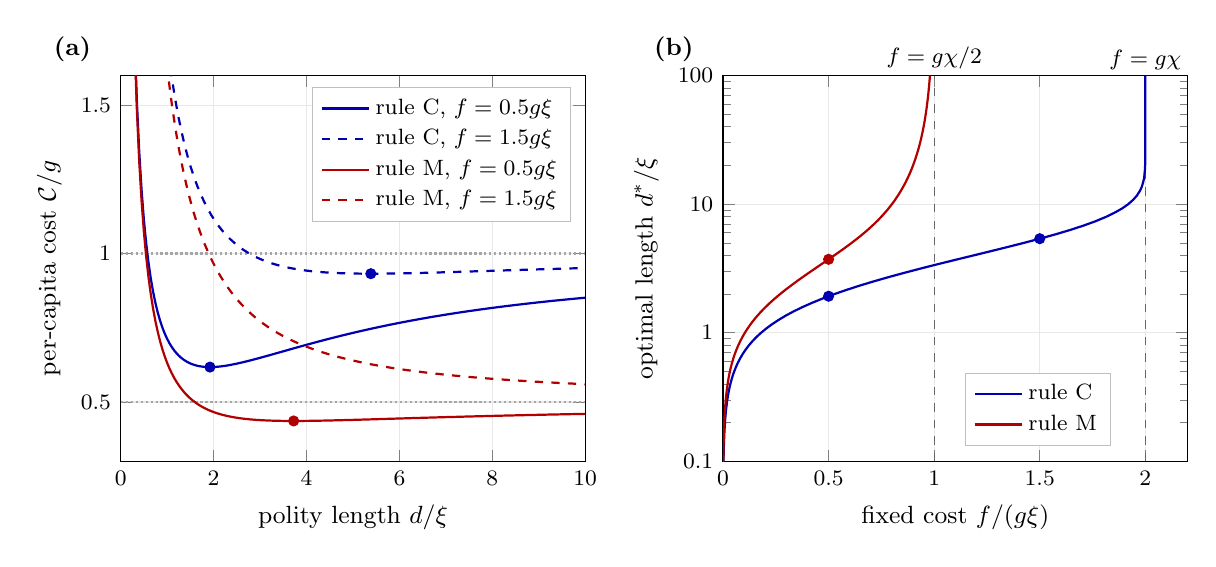
\begin{tikzpicture}
  \begin{axis}[name=pa, scale only axis, width=5.9cm, height=4.9cm,
      xmin=0, xmax=10, ymin=0.3, ymax=1.6,
      xlabel={polity length $d/\xi$}, ylabel={per-capita cost $\mathcal C/g$},
      grid=major, grid style={gray!18},
      legend style={font=\footnotesize, at={(0.97,0.97)}, anchor=north east, draw=gray!50, fill=white, cells={anchor=west}},
      every axis label/.style={font=\small}, tick label style={font=\footnotesize}]
    \draw[gray!70, densely dotted, thick] (axis cs:0,1) -- (axis cs:10,1);
    \draw[gray!70, densely dotted, thick] (axis cs:0,0.5) -- (axis cs:10,0.5);
    \addplot[blue!70!black, thick] coordinates {(0.2,2.548) (0.25,2.06) (0.3,1.738) (0.35,1.511) (0.4,1.344) (0.45,1.216) (0.5,1.115) (0.55,1.035) (0.6,0.9694) (0.65,0.9155) (0.7,0.8705) (0.75,0.8328) (0.8,0.8008) (0.85,0.7736) (0.9,0.7503) (0.95,0.7303) (1,0.7131) (1.05,0.6982) (1.1,0.6854) (1.15,0.6743) (1.2,0.6647) (1.25,0.6564) (1.3,0.6493) (1.35,0.6432) (1.4,0.638) (1.45,0.6336) (1.5,0.6298) (1.55,0.6267) (1.6,0.6242) (1.65,0.6221) (1.7,0.6205) (1.75,0.6193) (1.8,0.6184) (1.85,0.6179) (1.9,0.6176) (1.95,0.6176) (2,0.6179) (2.05,0.6183) (2.1,0.619) (2.15,0.6198) (2.2,0.6208) (2.25,0.6219) (2.3,0.6232) (2.35,0.6245) (2.4,0.626) (2.45,0.6276) (2.5,0.6292) (2.55,0.6309) (2.6,0.6327) (2.65,0.6346) (2.7,0.6365) (2.75,0.6384) (2.8,0.6404) (2.85,0.6425) (2.9,0.6445) (2.95,0.6466) (3,0.6488) (3.05,0.6509) (3.1,0.6531) (3.15,0.6552) (3.2,0.6574) (3.25,0.6596) (3.3,0.6618) (3.35,0.6641) (3.4,0.6663) (3.45,0.6685) (3.5,0.6707) (3.55,0.6729) (3.6,0.6752) (3.65,0.6774) (3.7,0.6796) (3.75,0.6818) (3.8,0.684) (3.85,0.6862) (3.9,0.6883) (3.95,0.6905) (4,0.6927) (4.05,0.6948) (4.1,0.6969) (4.15,0.6991) (4.2,0.7012) (4.25,0.7033) (4.3,0.7053) (4.35,0.7074) (4.4,0.7095) (4.45,0.7115) (4.5,0.7135) (4.55,0.7155) (4.6,0.7175) (4.65,0.7195) (4.7,0.7214) (4.75,0.7234) (4.8,0.7253) (4.85,0.7272) (4.9,0.7291) (4.95,0.731) (5,0.7328) (5.05,0.7347) (5.1,0.7365) (5.15,0.7383) (5.2,0.7401) (5.25,0.7419) (5.3,0.7436) (5.35,0.7454) (5.4,0.7471) (5.45,0.7488) (5.5,0.7505) (5.55,0.7522) (5.6,0.7539) (5.65,0.7555) (5.7,0.7571) (5.75,0.7588) (5.8,0.7604) (5.85,0.7619) (5.9,0.7635) (5.95,0.7651) (6,0.7666) (6.05,0.7681) (6.1,0.7696) (6.15,0.7711) (6.2,0.7726) (6.25,0.7741) (6.3,0.7755) (6.35,0.7769) (6.4,0.7784) (6.45,0.7798) (6.5,0.7812) (6.55,0.7825) (6.6,0.7839) (6.65,0.7853) (6.7,0.7866) (6.75,0.7879) (6.8,0.7892) (6.85,0.7905) (6.9,0.7918) (6.95,0.7931) (7,0.7943) (7.05,0.7956) (7.1,0.7968) (7.15,0.798) (7.2,0.7993) (7.25,0.8005) (7.3,0.8016) (7.35,0.8028) (7.4,0.804) (7.45,0.8051) (7.5,0.8063) (7.55,0.8074) (7.6,0.8085) (7.65,0.8096) (7.7,0.8107) (7.75,0.8118) (7.8,0.8129) (7.85,0.8139) (7.9,0.815) (7.95,0.816) (8,0.8171) (8.05,0.8181) (8.1,0.8191) (8.15,0.8201) (8.2,0.8211) (8.25,0.8221) (8.3,0.8231) (8.35,0.824) (8.4,0.825) (8.45,0.8259) (8.5,0.8269) (8.55,0.8278) (8.6,0.8287) (8.65,0.8296) (8.7,0.8306) (8.75,0.8314) (8.8,0.8323) (8.85,0.8332) (8.9,0.8341) (8.95,0.8349) (9,0.8358) (9.05,0.8366) (9.1,0.8375) (9.15,0.8383) (9.2,0.8391) (9.25,0.84) (9.3,0.8408) (9.35,0.8416) (9.4,0.8424) (9.45,0.8431) (9.5,0.8439) (9.55,0.8447) (9.6,0.8455) (9.65,0.8462) (9.7,0.847) (9.75,0.8477) (9.8,0.8485) (9.85,0.8492) (9.9,0.8499) (9.95,0.8506) (10,0.8513)};
    \addlegendentry{rule C, $f=0.5g\xi$}
    \addplot[blue!70!black, thick, dashed] coordinates {(0.55,2.853) (0.6,2.636) (0.65,2.454) (0.7,2.299) (0.75,2.166) (0.8,2.051) (0.85,1.95) (0.9,1.861) (0.95,1.783) (1,1.713) (1.05,1.651) (1.1,1.594) (1.15,1.544) (1.2,1.498) (1.25,1.456) (1.3,1.419) (1.35,1.384) (1.4,1.352) (1.45,1.323) (1.5,1.296) (1.55,1.272) (1.6,1.249) (1.65,1.228) (1.7,1.209) (1.75,1.191) (1.8,1.174) (1.85,1.158) (1.9,1.144) (1.95,1.13) (2,1.118) (2.05,1.106) (2.1,1.095) (2.15,1.085) (2.2,1.075) (2.25,1.066) (2.3,1.058) (2.35,1.05) (2.4,1.043) (2.45,1.036) (2.5,1.029) (2.55,1.023) (2.6,1.017) (2.65,1.012) (2.7,1.007) (2.75,1.002) (2.8,0.9976) (2.85,0.9933) (2.9,0.9894) (2.95,0.9856) (3,0.9821) (3.05,0.9788) (3.1,0.9756) (3.15,0.9727) (3.2,0.9699) (3.25,0.9673) (3.3,0.9649) (3.35,0.9626) (3.4,0.9604) (3.45,0.9584) (3.5,0.9564) (3.55,0.9546) (3.6,0.9529) (3.65,0.9514) (3.7,0.9499) (3.75,0.9485) (3.8,0.9471) (3.85,0.9459) (3.9,0.9448) (3.95,0.9437) (4,0.9427) (4.05,0.9417) (4.1,0.9408) (4.15,0.94) (4.2,0.9393) (4.25,0.9386) (4.3,0.9379) (4.35,0.9373) (4.4,0.9367) (4.45,0.9362) (4.5,0.9357) (4.55,0.9353) (4.6,0.9349) (4.65,0.9345) (4.7,0.9342) (4.75,0.9339) (4.8,0.9336) (4.85,0.9334) (4.9,0.9332) (4.95,0.933) (5,0.9328) (5.05,0.9327) (5.1,0.9326) (5.15,0.9325) (5.2,0.9324) (5.25,0.9324) (5.3,0.9323) (5.35,0.9323) (5.4,0.9323) (5.45,0.9323) (5.5,0.9323) (5.55,0.9324) (5.6,0.9324) (5.65,0.9325) (5.7,0.9326) (5.75,0.9327) (5.8,0.9328) (5.85,0.9329) (5.9,0.933) (5.95,0.9331) (6,0.9333) (6.05,0.9334) (6.1,0.9336) (6.15,0.9337) (6.2,0.9339) (6.25,0.9341) (6.3,0.9342) (6.35,0.9344) (6.4,0.9346) (6.45,0.9348) (6.5,0.935) (6.55,0.9352) (6.6,0.9354) (6.65,0.9356) (6.7,0.9358) (6.75,0.9361) (6.8,0.9363) (6.85,0.9365) (6.9,0.9367) (6.95,0.937) (7,0.9372) (7.05,0.9374) (7.1,0.9377) (7.15,0.9379) (7.2,0.9381) (7.25,0.9384) (7.3,0.9386) (7.35,0.9389) (7.4,0.9391) (7.45,0.9394) (7.5,0.9396) (7.55,0.9399) (7.6,0.9401) (7.65,0.9403) (7.7,0.9406) (7.75,0.9408) (7.8,0.9411) (7.85,0.9413) (7.9,0.9416) (7.95,0.9418) (8,0.9421) (8.05,0.9423) (8.1,0.9426) (8.15,0.9428) (8.2,0.9431) (8.25,0.9433) (8.3,0.9436) (8.35,0.9438) (8.4,0.944) (8.45,0.9443) (8.5,0.9445) (8.55,0.9448) (8.6,0.945) (8.65,0.9453) (8.7,0.9455) (8.75,0.9457) (8.8,0.946) (8.85,0.9462) (8.9,0.9464) (8.95,0.9467) (9,0.9469) (9.05,0.9471) (9.1,0.9474) (9.15,0.9476) (9.2,0.9478) (9.25,0.9481) (9.3,0.9483) (9.35,0.9485) (9.4,0.9487) (9.45,0.949) (9.5,0.9492) (9.55,0.9494) (9.6,0.9496) (9.65,0.9499) (9.7,0.9501) (9.75,0.9503) (9.8,0.9505) (9.85,0.9507) (9.9,0.9509) (9.95,0.9511) (10,0.9513)};
    \addlegendentry{rule C, $f=1.5g\xi$}
    \addplot[red!70!black, thick] coordinates {(0.2,2.532) (0.25,2.039) (0.3,1.713) (0.35,1.482) (0.4,1.31) (0.45,1.178) (0.5,1.074) (0.55,0.9894) (0.6,0.92) (0.65,0.862) (0.7,0.8131) (0.75,0.7713) (0.8,0.7354) (0.85,0.7043) (0.9,0.6771) (0.95,0.6532) (1,0.6321) (1.05,0.6134) (1.1,0.5968) (1.15,0.5819) (1.2,0.5686) (1.25,0.5566) (1.3,0.5458) (1.35,0.5361) (1.4,0.5272) (1.45,0.5192) (1.5,0.5119) (1.55,0.5053) (1.6,0.4993) (1.65,0.4937) (1.7,0.4887) (1.75,0.4841) (1.8,0.4798) (1.85,0.476) (1.9,0.4724) (1.95,0.4692) (2,0.4662) (2.05,0.4634) (2.1,0.4609) (2.15,0.4586) (2.2,0.4564) (2.25,0.4545) (2.3,0.4527) (2.35,0.451) (2.4,0.4495) (2.45,0.4481) (2.5,0.4469) (2.55,0.4457) (2.6,0.4446) (2.65,0.4437) (2.7,0.4428) (2.75,0.442) (2.8,0.4412) (2.85,0.4406) (2.9,0.4399) (2.95,0.4394) (3,0.4389) (3.05,0.4385) (3.1,0.4381) (3.15,0.4377) (3.2,0.4374) (3.25,0.4372) (3.3,0.4369) (3.35,0.4367) (3.4,0.4366) (3.45,0.4364) (3.5,0.4363) (3.55,0.4362) (3.6,0.4362) (3.65,0.4361) (3.7,0.4361) (3.75,0.4361) (3.8,0.4361) (3.85,0.4362) (3.9,0.4362) (3.95,0.4363) (4,0.4364) (4.05,0.4364) (4.1,0.4366) (4.15,0.4367) (4.2,0.4368) (4.25,0.4369) (4.3,0.4371) (4.35,0.4372) (4.4,0.4374) (4.45,0.4375) (4.5,0.4377) (4.55,0.4379) (4.6,0.4381) (4.65,0.4383) (4.7,0.4385) (4.75,0.4387) (4.8,0.4389) (4.85,0.4391) (4.9,0.4393) (4.95,0.4395) (5,0.4397) (5.05,0.44) (5.1,0.4402) (5.15,0.4404) (5.2,0.4406) (5.25,0.4409) (5.3,0.4411) (5.35,0.4413) (5.4,0.4415) (5.45,0.4418) (5.5,0.442) (5.55,0.4422) (5.6,0.4425) (5.65,0.4427) (5.7,0.443) (5.75,0.4432) (5.8,0.4434) (5.85,0.4437) (5.9,0.4439) (5.95,0.4441) (6,0.4444) (6.05,0.4446) (6.1,0.4448) (6.15,0.4451) (6.2,0.4453) (6.25,0.4456) (6.3,0.4458) (6.35,0.446) (6.4,0.4462) (6.45,0.4465) (6.5,0.4467) (6.55,0.4469) (6.6,0.4472) (6.65,0.4474) (6.7,0.4476) (6.75,0.4478) (6.8,0.4481) (6.85,0.4483) (6.9,0.4485) (6.95,0.4487) (7,0.449) (7.05,0.4492) (7.1,0.4494) (7.15,0.4496) (7.2,0.4498) (7.25,0.45) (7.3,0.4503) (7.35,0.4505) (7.4,0.4507) (7.45,0.4509) (7.5,0.4511) (7.55,0.4513) (7.6,0.4515) (7.65,0.4517) (7.7,0.4519) (7.75,0.4521) (7.8,0.4523) (7.85,0.4525) (7.9,0.4527) (7.95,0.4529) (8,0.4531) (8.05,0.4533) (8.1,0.4535) (8.15,0.4537) (8.2,0.4539) (8.25,0.4541) (8.3,0.4543) (8.35,0.4545) (8.4,0.4546) (8.45,0.4548) (8.5,0.455) (8.55,0.4552) (8.6,0.4554) (8.65,0.4556) (8.7,0.4557) (8.75,0.4559) (8.8,0.4561) (8.85,0.4563) (8.9,0.4564) (8.95,0.4566) (9,0.4568) (9.05,0.457) (9.1,0.4571) (9.15,0.4573) (9.2,0.4575) (9.25,0.4576) (9.3,0.4578) (9.35,0.458) (9.4,0.4581) (9.45,0.4583) (9.5,0.4584) (9.55,0.4586) (9.6,0.4588) (9.65,0.4589) (9.7,0.4591) (9.75,0.4592) (9.8,0.4594) (9.85,0.4595) (9.9,0.4597) (9.95,0.4598) (10,0.46)};
    \addlegendentry{rule M, $f=0.5g\xi$}
    \addplot[red!70!black, thick, dashed] coordinates {(0.55,2.808) (0.6,2.587) (0.65,2.4) (0.7,2.242) (0.75,2.105) (0.8,1.985) (0.85,1.881) (0.9,1.788) (0.95,1.706) (1,1.632) (1.05,1.566) (1.1,1.506) (1.15,1.452) (1.2,1.402) (1.25,1.357) (1.3,1.315) (1.35,1.277) (1.4,1.242) (1.45,1.209) (1.5,1.179) (1.55,1.15) (1.6,1.124) (1.65,1.1) (1.7,1.077) (1.75,1.056) (1.8,1.035) (1.85,1.017) (1.9,0.9987) (1.95,0.982) (2,0.9662) (2.05,0.9512) (2.1,0.9371) (2.15,0.9237) (2.2,0.911) (2.25,0.8989) (2.3,0.8875) (2.35,0.8766) (2.4,0.8662) (2.45,0.8563) (2.5,0.8469) (2.55,0.8379) (2.6,0.8292) (2.65,0.821) (2.7,0.8131) (2.75,0.8056) (2.8,0.7984) (2.85,0.7914) (2.9,0.7848) (2.95,0.7784) (3,0.7722) (3.05,0.7663) (3.1,0.7607) (3.15,0.7552) (3.2,0.7499) (3.25,0.7448) (3.3,0.74) (3.35,0.7352) (3.4,0.7307) (3.45,0.7263) (3.5,0.722) (3.55,0.7179) (3.6,0.7139) (3.65,0.7101) (3.7,0.7064) (3.75,0.7028) (3.8,0.6993) (3.85,0.6959) (3.9,0.6926) (3.95,0.6894) (4,0.6864) (4.05,0.6834) (4.1,0.6805) (4.15,0.6776) (4.2,0.6749) (4.25,0.6722) (4.3,0.6696) (4.35,0.6671) (4.4,0.6647) (4.45,0.6623) (4.5,0.6599) (4.55,0.6577) (4.6,0.6555) (4.65,0.6533) (4.7,0.6512) (4.75,0.6492) (4.8,0.6472) (4.85,0.6453) (4.9,0.6434) (4.95,0.6415) (5,0.6397) (5.05,0.638) (5.1,0.6363) (5.15,0.6346) (5.2,0.6329) (5.25,0.6313) (5.3,0.6298) (5.35,0.6282) (5.4,0.6267) (5.45,0.6253) (5.5,0.6238) (5.55,0.6224) (5.6,0.6211) (5.65,0.6197) (5.7,0.6184) (5.75,0.6171) (5.8,0.6158) (5.85,0.6146) (5.9,0.6134) (5.95,0.6122) (6,0.611) (6.05,0.6099) (6.1,0.6088) (6.15,0.6077) (6.2,0.6066) (6.25,0.6056) (6.3,0.6045) (6.35,0.6035) (6.4,0.6025) (6.45,0.6015) (6.5,0.6006) (6.55,0.5996) (6.6,0.5987) (6.65,0.5978) (6.7,0.5969) (6.75,0.596) (6.8,0.5951) (6.85,0.5943) (6.9,0.5934) (6.95,0.5926) (7,0.5918) (7.05,0.591) (7.1,0.5902) (7.15,0.5895) (7.2,0.5887) (7.25,0.588) (7.3,0.5872) (7.35,0.5865) (7.4,0.5858) (7.45,0.5851) (7.5,0.5844) (7.55,0.5838) (7.6,0.5831) (7.65,0.5824) (7.7,0.5818) (7.75,0.5812) (7.8,0.5805) (7.85,0.5799) (7.9,0.5793) (7.95,0.5787) (8,0.5781) (8.05,0.5775) (8.1,0.577) (8.15,0.5764) (8.2,0.5758) (8.25,0.5753) (8.3,0.5748) (8.35,0.5742) (8.4,0.5737) (8.45,0.5732) (8.5,0.5727) (8.55,0.5722) (8.6,0.5717) (8.65,0.5712) (8.7,0.5707) (8.75,0.5702) (8.8,0.5697) (8.85,0.5693) (8.9,0.5688) (8.95,0.5683) (9,0.5679) (9.05,0.5675) (9.1,0.567) (9.15,0.5666) (9.2,0.5662) (9.25,0.5657) (9.3,0.5653) (9.35,0.5649) (9.4,0.5645) (9.45,0.5641) (9.5,0.5637) (9.55,0.5633) (9.6,0.5629) (9.65,0.5626) (9.7,0.5622) (9.75,0.5618) (9.8,0.5614) (9.85,0.5611) (9.9,0.5607) (9.95,0.5604) (10,0.56)};
    \addlegendentry{rule M, $f=1.5g\xi$}
    \addplot[only marks, mark=*, mark size=1.8pt, blue!70!black, forget plot] coordinates {(1.9226,0.6176) (5.3853,0.9323)};
    \addplot[only marks, mark=*, mark size=1.8pt, red!70!black, forget plot] coordinates {(3.7236,0.4361)};
  \end{axis}
  \node[font=\small\bfseries, anchor=south east] at ($(pa.north west)+(-0.25cm,0.05cm)$) {(a)};
  \begin{semilogyaxis}[name=pb, at={($(pa.south east)+(1.75cm,0)$)}, anchor=south west, scale only axis, width=5.9cm, height=4.9cm,
      xmin=0, xmax=2.2, ymin=0.1, ymax=100, clip mode=individual,
      log ticks with fixed point,
      xlabel={fixed cost $f/(g\xi)$}, ylabel={optimal length $d^\ast/\xi$},
      grid=major, grid style={gray!18},
      legend style={font=\footnotesize, at={(0.52,0.04)}, anchor=south west, draw=gray!50, fill=white, cells={anchor=west}},
      every axis label/.style={font=\small}, tick label style={font=\footnotesize}]
    \draw[black!60, dashed] (axis cs:1,0.1) -- (axis cs:1,100);
    \draw[black!60, dashed] (axis cs:2,0.1) -- (axis cs:2,100);
    \node[font=\footnotesize, anchor=south, inner sep=2pt] at (axis cs:1,100) {$f=g\chi/2$};
    \node[font=\footnotesize, anchor=south, inner sep=2pt] at (axis cs:2,100) {$f=g\chi$};
    \addplot[blue!70!black, thick] coordinates {(0.0006147,0.05) (0.0007157,0.05399) (0.0008333,0.0583) (0.0009702,0.06295) (0.001129,0.06797) (0.001314,0.0734) (0.00153,0.07926) (0.00178,0.08558) (0.00207,0.09241) (0.002408,0.09978) (0.0028,0.1077) (0.003256,0.1163) (0.003784,0.1256) (0.004398,0.1357) (0.005109,0.1465) (0.005934,0.1582) (0.00689,0.1708) (0.007998,0.1844) (0.00928,0.1991) (0.01076,0.215) (0.01248,0.2322) (0.01446,0.2507) (0.01675,0.2707) (0.01939,0.2923) (0.02244,0.3157) (0.02595,0.3409) (0.02998,0.3681) (0.03462,0.3974) (0.03995,0.4291) (0.04607,0.4634) (0.05307,0.5004) (0.06108,0.5403) (0.07022,0.5834) (0.08065,0.63) (0.09251,0.6802) (0.106,0.7345) (0.1213,0.7931) (0.1385,0.8564) (0.158,0.9248) (0.18,0.9986) (0.2046,1.078) (0.2321,1.164) (0.2628,1.257) (0.2969,1.358) (0.3347,1.466) (0.3763,1.583) (0.4219,1.709) (0.4717,1.846) (0.5258,1.993) (0.5843,2.152) (0.647,2.324) (0.714,2.509) (0.7848,2.709) (0.8592,2.925) (0.9368,3.159) (1.017,3.411) (1.099,3.683) (1.182,3.977) (1.265,4.294) (1.347,4.637) (1.427,5.007) (1.504,5.407) (1.577,5.838) (1.645,6.304) (1.707,6.807) (1.763,7.35) (1.812,7.937) (1.854,8.57) (1.89,9.254) (1.919,9.993) (1.942,10.79) (1.96,11.65) (1.973,12.58) (1.983,13.59) (1.989,14.67) (1.994,15.84) (1.996,17.1) (1.998,18.47) (1.999,19.94) (2,21.53) (2,23.25) (2,25.11) (2,27.11) (2,29.28) (2,31.61) (2,34.13) (2,36.86) (2,39.8) (2,42.98) (2,46.4) (2,50.11) (2,54.11) (2,58.42) (2,63.09) (2,68.12) (2,73.56) (2,79.43) (2,85.77) (2,92.61) (2,100)};
    \addlegendentry{rule C}
    \addplot[red!70!black, thick] coordinates {(0.0005823,0.06) (0.0006862,0.06522) (0.0008084,0.07088) (0.0009521,0.07705) (0.001121,0.08374) (0.00132,0.09102) (0.001553,0.09894) (0.001827,0.1075) (0.002148,0.1169) (0.002526,0.127) (0.002967,0.1381) (0.003485,0.1501) (0.004091,0.1631) (0.0048,0.1773) (0.005628,0.1927) (0.006594,0.2095) (0.007721,0.2277) (0.009034,0.2475) (0.01056,0.269) (0.01234,0.2924) (0.0144,0.3178) (0.01678,0.3454) (0.01954,0.3755) (0.02273,0.4081) (0.0264,0.4436) (0.03062,0.4821) (0.03546,0.524) (0.041,0.5696) (0.04733,0.6191) (0.05452,0.6729) (0.06268,0.7314) (0.07191,0.795) (0.08231,0.8641) (0.09397,0.9392) (0.107,1.021) (0.1215,1.11) (0.1375,1.206) (0.1552,1.311) (0.1745,1.425) (0.1956,1.549) (0.2183,1.683) (0.2428,1.83) (0.2688,1.989) (0.2964,2.162) (0.3254,2.349) (0.3555,2.554) (0.3867,2.776) (0.4185,3.017) (0.4507,3.279) (0.4831,3.564) (0.5153,3.874) (0.5469,4.211) (0.5778,4.577) (0.6077,4.975) (0.6363,5.407) (0.6635,5.877) (0.6891,6.388) (0.7132,6.944) (0.7357,7.547) (0.7565,8.203) (0.7759,8.916) (0.7937,9.691) (0.8102,10.53) (0.8253,11.45) (0.8393,12.44) (0.8521,13.53) (0.864,14.7) (0.8748,15.98) (0.8849,17.37) (0.8941,18.88) (0.9025,20.52) (0.9103,22.3) (0.9175,24.24) (0.9241,26.35) (0.9302,28.64) (0.9358,31.13) (0.9409,33.84) (0.9456,36.78) (0.95,39.98) (0.954,43.45) (0.9577,47.23) (0.961,51.33) (0.9642,55.8) (0.967,60.65) (0.9697,65.92) (0.9721,71.65) (0.9743,77.88) (0.9764,84.64) (0.9783,92) (0.98,100)};
    \addlegendentry{rule M}
    \addplot[only marks, mark=*, mark size=1.8pt, blue!70!black, forget plot] coordinates {(0.5,1.9226) (1.5,5.3853)};
    \addplot[only marks, mark=*, mark size=1.8pt, red!70!black, forget plot] coordinates {(0.5,3.7236)};
  \end{semilogyaxis}
  \node[font=\small\bfseries, anchor=south east] at ($(pb.north west)+(-0.25cm,0.05cm)$) {(b)};
\end{tikzpicture}

  \caption{\textbf{Polity size on the line under the two policy rules.} Preferences have correlation $\Gamma(z)=e^{-\lvert z\rvert/\xi}$, so $\chi=2\xi$. (a) Per-capita cost against the length $d$ of an interval polity, centered at its designated member under rule C, at the fixed costs $f=0.5g\xi$ and $f=1.5g\xi$; dots mark the optima, and the dotted lines are the costs $g$ and $g/2$ of unbounded polities under rules C and M. At $f=0.5g\xi$ both rules have finite optima, and the one under rule M is $1.94$ times longer; at $f=1.5g\xi$ only rule C has one, while the cost under rule M decreases with length toward $g/2$. (b) Optimal length against $f/(g\xi)$ from the root equations of \cref{prop:abs-polity}(c). Rule M has a finite optimum only for $f<g\chi/2$ and rule C only for $f<g\chi$. Where both exist the optimum under rule M is the longer, as \cref{prop:abs-polity}(d) states, by a factor that tends to $\sqrt6/2$ at small fixed cost, increases along the computed grid and diverges at the rule-M threshold (\cref{chk:abs-polity}). Near its own threshold the optimal length diverges as a power of the remaining margin under rule M and logarithmically under rule C.}
  \label{fig:abs-polity}
\end{figure}

Readings of the criterion, of Deutsch's account of a people and of print as a durable medium of long range are in the Supplement (\cref{sup:abs-nations-readings}, with \cref{rem:abs-polity-readings}); conquest, conflict and contingency, which shape actual borders, are outside the model.

Cities are treated in the Supplement (\cref{sec:abs-cities}) through the co-presence modality. Under the hypotheses stated there, a set of agents every pair of which can meet within one round has diameter at most the travel speed times the travel time per round (\cref{prop:abs-one-round}), and this reach composes with the size bound on the extent of a collective (\cref{cor:abs-one-round-extent}). Such a set is defined without contrast and need not be a collective.

\subsection{Distance and scale-free coherence}\label{sec:abs-distance}

The persistence of the distance effect in trade as communication improved, summarized with its sources in the Supplement (\cref{sup:abs-the-distance-effect-in-trade-sources}), is read here through the dependence of the elasticity of coherence on its scale.

The distance elasticity of a coherence profile $\Psi(d/\xi)$ is the same for every $\xi$ at each fixed distance if and only if the profile is a power law, while for the profile $K_0$ of diffusion with leak in two dimensions a longer $\xi$ lowers it at every fixed distance (Supplement, \cref{prop:abs-elasticity}). Scale-free coherence arises from nested coupling, such as administrative and economic hierarchies may provide.

\begin{proposition}[Nested coupling gives scale-free coherence]\label{prop:abs-hierarchy}
Let $N=b^{n_{\mathrm H}}$ agents, $b\ge2$, be organized in nested blocks of sizes $b,b^2,\dots,b^{n_{\mathrm H}}$; let two agents whose smallest common block has level $l$ be coupled with weight $a^{\mathrm H}_l=A_{\mathrm h}\mathfrak q^{l-1}/[(b-1)b^{l-1}]$, so that each agent's total coupling to its level-$l$ cousins is $A_{\mathrm h}\mathfrak q^{l-1}$; and let every agent have precision leak $\varepsilon^\Pi>0$, so that the world-conditional precision is $\Pi=\varepsilon^\Pi I+L$ with $L$ the weighted Laplacian of the couplings $a^\Pi_{ij}=a^{\mathrm H}_l$, and let $\mathsf G=\Pi^{-1}$.
\begin{enumerate}
\item[(a)] $\mathsf G(i,j)$ depends only on the level $l$ of the pair. With $\mathsf g_l=\sum_{l'=l}^{n_{\mathrm H}}A_{\mathrm h}\mathfrak q^{l'-1}+A_{\mathrm h}\mathfrak q^{l-1}/(b-1)$,
\[
\mathsf G(l)=\frac{b^{-n_{\mathrm H}}}{\varepsilon^\Pi}+\sum_{l'=l+1}^{n_{\mathrm H}}\frac{(b-1)b^{-l'}}{\varepsilon^\Pi+\mathsf g_{l'}}-\frac{b^{-l}}{\varepsilon^\Pi+\mathsf g_l}\quad(1\le l\le n_{\mathrm H}),\qquad\mathsf G(0)=\frac{b^{-n_{\mathrm H}}}{\varepsilon^\Pi}+\sum_{l'=1}^{n_{\mathrm H}}\frac{(b-1)b^{-l'}}{\varepsilon^\Pi+\mathsf g_{l'}}.
\]
\item[(b)] If $1/b<\mathfrak q<1$, the correlation $\mathsf G(l)/\mathsf G(0)$ of a level-$l$ pair converges, as $n_{\mathrm H}\to\infty$ and then $\varepsilon^\Pi\to0$, to
\[
\frac{b(1-\mathfrak q)}{b-1}(b\mathfrak q)^{-l}\qquad(l\ge1),
\]
so correlations fall by the factor $1/(b\mathfrak q)$ per level.
\item[(c)] If level-$l$ pairs lie at distance $d_l=d_1b^{(l-1)/D_e}$, as for blocks of linear size proportional to $b^{l/D_e}$ in $D_e$ dimensions, the limit in (b) is proportional to $d_l^{-\alpha_{\mathrm H}}$ with $\alpha_{\mathrm H}=D_e\ln(b\mathfrak q)/\ln b$. The exponent does not depend on $A_{\mathrm h}$ or on the unit of distance; only the allocation of coupling across levels, $\mathfrak q$, and the branching $b$ change it.
\end{enumerate}
\end{proposition}
% src: L5-P15; (b) restated as an exact double limit

Proof in \cref{app:abs}; the spectral formula and the limit were checked numerically (\cref{chk:abs-hierarchy}). The nested medium renormalizes exactly: the coordinates of its level-one blocks follow a nested medium on $b^{n_{\mathrm H}-1}$ agents with $A_{\mathrm h}$ multiplied by $\mathfrak q$, the contrast of a block is the same in the coarse medium of every level below its own, the level up to which blocks reach a declared contrast is explicit, and $\alpha_{\mathrm H}$ is $D_e$ minus the renormalization exponent of the leak ratio (\cref{thm:ren-nested}). Against exchangeable comparison media, which a medium without declared geometry requires, no block of any level is a collective at any leak when $\mathfrak q\ge1/b$, whether judged in the level-zero medium or level by level (\cref{prop:ren-per-level}(d)), so the scale-free coherence of (b) comes without nested collectives unless a geometry is declared; with the sixteen agents of one such medium placed on $\Z$ and the lattice clause at every level, an exhaustive enumeration found collectives at all three levels for $\mathfrak q\le0.55$ at strong enough grounding, and the general embedding is open (\cref{sec:ren-levels}).

Cutoffs at finite leak and a log-periodic modulation in a computed small hierarchy are described in the Supplement (\cref{rem:abs-cutoff}). It is conjectured (\cref{conj:abs-distance}) that the persistence of the distance elasticity, which one coherence scale lengthened by communication does not fit as the dominant mechanism, fits two readings: a binding modality whose range did not grow, or scale-free coherence in the binding modality.

Unconditional correlations count the common response to shared shocks as coherence. When the unconditional covariance is the world-conditional one plus a common mode, the ultrametric contrast computed from unconditional correlations is bounded, under the hypotheses stated there, by a cap that depends only on the ratio of the largest world-conditional variance to the variance of the common mode (Supplement, \cref{prop:abs-ultrametric-cap}, in \cref{sec:abs-world}), which is why the diagnostic uses world-conditional correlations.

\subsection{Abstract collectives as graded meta-agents}\label{sec:abs-graded}

Hypothesis H1 in its final form (\cref{thm:agy-h1}) grades meta-agenthood by a boundary, contrast at a declared level above the baseline, closure, interaction necessity and agency (\cref{def:agy-meta-agent}). \Cref{tab:abs-graded} says which of these can be checked in a stated model for each abstract collective and which remain interpretation.

\begin{table}[t]
\centering\small
\caption{Abstract collectives against the properties of hypothesis H1. Entries that cite a result can be checked in the stated model; the rest are interpretation or are not addressed.}
\label{tab:abs-graded}
\begin{tabular}{@{}>{\raggedright\arraybackslash}p{0.11\textwidth}>{\raggedright\arraybackslash}p{0.25\textwidth}>{\raggedright\arraybackslash}p{0.17\textwidth}>{\raggedright\arraybackslash}p{0.19\textwidth}>{\raggedright\arraybackslash}p{0.15\textwidth}@{}}
\toprule
Collective & Boundary and contrast & Closure & Interaction necessity & Agency\\
\midrule
Culture (convention) & Strong barriers give ultrametric contrast in the computed ring (\cref{chk:abs-barrier}); \cref{prop:abs-barrier} gives the border factor; walls give domains (\cref{prop:abs-seguy}), spectral contrast open (\cref{open:abs-code-contrast}); archives placed by their writers (\cref{prop:col-records-partition}) & Records give slow memory (\cref{prop:sca-records-memory}); closure not shown & Contrast above one given the shared drive rules out separating nulls (\cref{prop:agy-nulls-vanish}(d)); decisive nulls not applied & Not claimed: no collective active states\\
Market (exchange) & Border factor and width (\cref{prop:abs-barrier}), bypass (\cref{prop:abs-bypass}); measured border effects are readings & A revealing price is sufficient (\cref{prop:abs-walras}(b)); dynamic closure not shown & As for cultures & None for the market; institutions can be checked against \cref{thm:agy-agency}\\
Polity (law) & Long-range borders need alignment (\cref{prop:abs-bypass}, \cref{conj:abs-alignment}); size criterion under a declared rule (\cref{prop:abs-polity}) & Statutes and registries give slow memory; closure not shown & Performative acts: the order parameter conditions on the shared drive (\cref{def:agy-order-parameter}); nulls not applied & Protocol of \cref{thm:agy-agency}; joint acts (\cref{thm:agy-joint-acts}); application is interpretation\\
City (co-presence) & One-round diameter (\cref{prop:abs-one-round}) composes with the size bound (\cref{cor:abs-one-round-extent}); no contrast result & Not addressed & Not addressed & Not addressed\\
\bottomrule
\end{tabular}
\end{table}

No abstract collective of this section is shown to meet every clause of \cref{def:agy-meta-agent}: the entries of \cref{tab:abs-graded} are established one clause at a time, in different models, and the decisive tests of \cref{def:agy-nulls} have been applied to none. Nothing here makes a culture or a market behave as if it minimized a group expected free energy, and nothing here derives the formation of a culture, a market or a polity: the propositions describe stationary structure under declared couplings, not its origin (\cref{sec:frm-status}). The discussion of each column of the table and the phenomena outside the framework's assumptions are in the Supplement (\cref{sup:abs-graded-meta-agents-discussion-and-open-p}).

The Supplement states three open problems: whether the code domains of the walled regimes have spectral contrast (\cref{open:abs-code-contrast}), whether allocating one attention capacity across modalities couples them (\cref{open:abs-attention}), and when an abstract collective with contrast and closure has agency in the sense of hypothesis H1 (\cref{open:abs-institutions}).

% Section 11 of "Communication, Coherence and Collective Agents".
\section{Meta-agents as agents}\label{sec:met}
% src: H3 (H3-D1 to H3-D5, H3-L0, H3-T1, H3-P1 to H3-P6, H3-X1 to H3-X3, H3-T2, H3-L2, H3-L3, H3-P4, H3-E1 to H3-E3, H3-T4, H3-R1 to H3-R8, H3 open items O1 to O7), H4-P10, H1-P3, HC_critic V2, V5, V6, V7, V10 and Sections 2.2 to 2.7, M_spec_H5 decisions 19 to 21 and Section 4

The meta-agents of \cref{sec:agy} are sets of agents selected by contrast and graded by closure, interaction necessity and agency. Hypothesis H5a asks that a meta-agent be an agent in the sense of \cref{sec:fw}, with internal, sensory, active and external states of its own, external states that obey a law of their own given its acts, internal states that encode a belief about them, and a joint act that follows a posterior over policies. In the author's example a corporation senses prices and the conduct of other firms, not a physical environment; we call the closed law of such coarse external states, given the coarse act, the meta-agent's abstract physics.

This section proves H5a as an exact conditional theorem in the linear-Gaussian framework (\cref{thm:met-h5a}), with coarse states declared as linear functions of the joint process \eqref{eq:col-joint}. The coarse sensory and active states form an exact path blanket when the sensory state is the information-form statistic of what the members sense; the coarse exterior has a closed law given the coarse act exactly when the kernel of its map is invariant under the exterior dynamics and the coarse exterior reads the members' channels only through the coarse act; the members' average estimate is then, up to their averaged computation noise, the predictive mean of the steady-state coarse filter at every number of consensus rounds, and that filter mean, with the steady-state covariance, parametrizes the meta-agent's predictive law from the centralized start with stationary initial covariance; and joint acts follow a group posterior. We compute what fails without each hypothesis (\cref{tab:met-hypotheses}). Error bounds exist for the blanket, the abstract physics and agency separately, and the Supplement proves an approximate form of the whole theorem for stable linear-Gaussian collectives, with the blanket conditions kept exact and the abstract physics relaxed to a declared model with defects (\cref{thm:apx-h5a,open:met-approximate}), and since no property uses contrast, H5a describes a meta-agent and selects none (\cref{rem:met-no-selection}). The examples of failing blanket conditions, the aggregate exteriors, the relations among the closure notions, the literal and level-0 aggregates, the two-firm model in which every property is computed and the open problems are in the Supplement (\cref{sup:met}).

Throughout, the joint process has per-channel noise, and stationary statements assume $\rho(A)<1$, under which it has a stationary law with finite second moments, the form that the moment bound (M) of \cref{asm:sca-standing} takes for it. Theorems are for linear-Gaussian models; discrete state spaces and nonlinear dynamics appear only as open problems. Messages from a meta-agent to its members are the subject of \cref{sec:hie}, and nothing here uses them.

\subsection{Coarse variables and the meta-agent's partition}\label{sec:met-coarse}

\begin{definition}[Coarse variables]\label{def:met-coarse}
Let $C$ be a set of $n$ agents with the canonical partition $(\sI,\sS,\sA,\sE)$ of \cref{def:col-partition} for the joint process \eqref{eq:col-joint}. Coarse variables of $C$ are declared before the analysis through linear maps $\mathsf P_{\mathrm I},\mathsf P_{\mathrm S},\mathsf P_{\mathrm A},\mathsf P_{\mathrm E}$ of full row rank,
\begin{equation}\label{eq:met-coarse}
y_C=\mathsf P_{\mathrm I}X_{\sI},\qquad s_C=\mathsf P_{\mathrm S}X_{\sS},\qquad a_C=\mathsf P_{\mathrm A}X_{\sA},\qquad\eta_C=\mathsf P_{\mathrm E}X_{\sE},\qquad b_C=(s_C,a_C)=\mathsf P_{\mathrm B}X_{\sB},
\end{equation}
the coarse internal, sensory, active and external states and the coarse blanket, with $\mathsf P_{\mathrm B}=\diag(\mathsf P_{\mathrm S},\mathsf P_{\mathrm A})$; $\mathsf P_{\mathrm I}$ is the map $\mathsf P$ of \cref{def:agy-closure}. When the sensory channels read the exterior through $\eta_C$, $A_{\sS\sE}=\mathcal H\mathsf P_{\mathrm E}$ with $\mathcal H$ of full column rank, the information-form sensory state is $s_C=\mathcal H^\top R_{\sS}^{-1}X_{\sS}$, where $R_{\sS}=Q^{\Xi}_{\sS\sS}$, and its information matrix is $\Lambda^s=\mathcal H^\top R_{\sS}^{-1}\mathcal H$.

(Normalizations.) For scalar member variables $x=(x_i)_{i\in C}$ one coarse coordinate has three normalizations: the average $\bar y_C=n^{-1}\one_C^\top x$, the unit-norm coordinate $\phi_C^\top x=n^{1/2}\bar y_C$ of \cref{def:col-contrast}, and the sum $\one_C^\top x$. For a partition into blocks $C_1,\dots,C_M$ the corresponding maps are the block-average map $\mathsf{Avg}$, with rows $n_j^{-1}\one_{C_j}^\top$, the block frame $\Phi$ of \cref{thm:col-bridge}, whose columns are the unit-norm block indicators $\phi_{C_j}$, and the block-sum matrix $\mathsf P$, with rows $\one_{C_j}^\top$; thus $\mathsf P=\diag(n_j)\mathsf{Avg}$ and $\Phi^\top=\diag(n_j^{-1/2})\mathsf P$.
\end{definition}
% src: H3-D1; M_spec_H5 Section 4 (coarse variables); HC_critic 2.4

The three normalizations have the same row space, on which alone exact closure depends (\cref{thm:met-abstract-physics}(c)), and closure defects, correlations and Markov errors are invariant under invertible rescaling of coarse coordinates, so every closure statement is the same in the three; contrast is always computed with $\phi_C$. \Cref{sec:hie,sec:ren,sec:env} use these conventions.

The sense in which the external states of a meta-agent are abstract, although every coarse variable is a function of the joint process, is discussed as an interpretation in the Supplement (\cref{rem:met-abstract}).

\subsection{The coarse blanket}\label{sec:met-blanket}

\begin{definition}[Coarse path blankets and residual assignments]\label{def:met-coarse-blanket}
On a window $[0,T]$ the weak coarse path blanket holds when $y_{C,0:T}\perp\eta_{C,0:T}\mid b_{C,0:T}$, and the strong coarse path blanket when $X_{\sI,0:T}\perp X_{\sE,0:T}\mid b_{C,0:T}$; the strong form implies the weak one for every $\mathsf P_{\mathrm I}$ and $\mathsf P_{\mathrm E}$. The coarse leak is $\iota^C_T=I(X_{\sI,0:T};X_{\sE,0:T}\mid b_{C,0:T})$ and the coarse leak rate is $\limsup_T\iota^C_T/T$, as in \cref{def:col-blankets}. A residual assignment completes $\mathsf P_{\mathrm B}$ to an invertible map $\mathcal T=(\mathsf P_{\mathrm B};\mathsf Z_{\mathrm{in}};\mathsf Z_{\mathrm{out}})$ of the blanket coordinates and places $\mathfrak r_{\mathrm{in}}=\mathsf Z_{\mathrm{in}}X_{\sB}$ with the interior and $\mathfrak r_{\mathrm{out}}=\mathsf Z_{\mathrm{out}}X_{\sB}$ with the exterior, giving the partition $\sI'=(X_{\sI},\mathfrak r_{\mathrm{in}})$, $\sB'=b_C$, $\sE'=(\mathfrak r_{\mathrm{out}},X_{\sE})$. With $\mathcal S$ equal to $\mathcal T$ on $X_{\sB}$ and to the identity elsewhere, $\tilde X=\mathcal SX$ follows \eqref{eq:col-joint} with $\tilde A=\mathcal SA\mathcal S^{-1}$ and $\tilde Q=\mathcal SQ^{\Xi}\mathcal S^\top\succ0$.
\end{definition}
% src: H3-D2

\begin{figure}[t]
  \centering
  % Figure: a meta-agent as an agent (def:met-coarse, def:met-coarse-blanket, thm:met-coarse-blanket,
% prop:met-sufficiency, thm:met-abstract-physics). Schematic; it plots no data. Notation and conditions as in sec:met.
% Left: three members of C (dashed box); each has one sensory channel (orange square, role S), one internal state mu_i
% (blue, role I) that exchanges messages with the other members (internal) and one active channel (red triangle,
% role A); the rows are the role groups X_S, X_I, X_A of the canonical partition. Right: the exterior X_E (gray).
% Double arrows: the declared coarse maps of full row rank, y_C = P_I X_I, s_C = P_S X_S, a_C = P_A X_A,
% eta_C = P_E X_E (eq:met-coarse), with the information-form statistic P_S = H^T R_S^{-1}. Dashed arrows: the
% residuals r_S = Z_S X_S and r_A = Z_A X_A that complete P_B = diag(P_S, P_A) to an invertible map, assigned to the
% interior side as in prop:met-sufficiency(a), so the partition is I' = (X_I, r_S, r_A), B' = b_C, E' = X_E. Center:
% the coarse blanket b_C = (s_C, a_C) between y_C and eta_C, with the coarse sensing s_{C,t+1} = Lambda^s eta_{C,t}
% + vbar_t, Lambda^s = H^T R_S^{-1} H, the coarse act entering the exterior through Bbar, and the closed law of
% eq:met-abstract-physics, eta_{C,t+1} = Fbar eta_{C,t} + Bbar a_{C,t} + wbar_t, exact when P_E A_EE = Fbar P_E
% (kernel invariance, thm:met-abstract-physics(c)) together with P_E A_ES = 0 and P_E A_EA = Bbar P_A, which the
% drawn couplings satisfy. Top line: the sensory channels read the exterior only through eta_C, A_SE = H P_E, and
% read no interior or active variable (a1, memoryless channels). Bottom line: the exterior reads the members only
% through the coarse act, A_EA = L_E P_A and A_ES = 0 (a2), so Bbar = P_E L_E (L_E is the sans-serif L_E of
% prop:met-sufficiency(a2), renamed from a calligraphic G_E that collided with the reserved graph symbol).
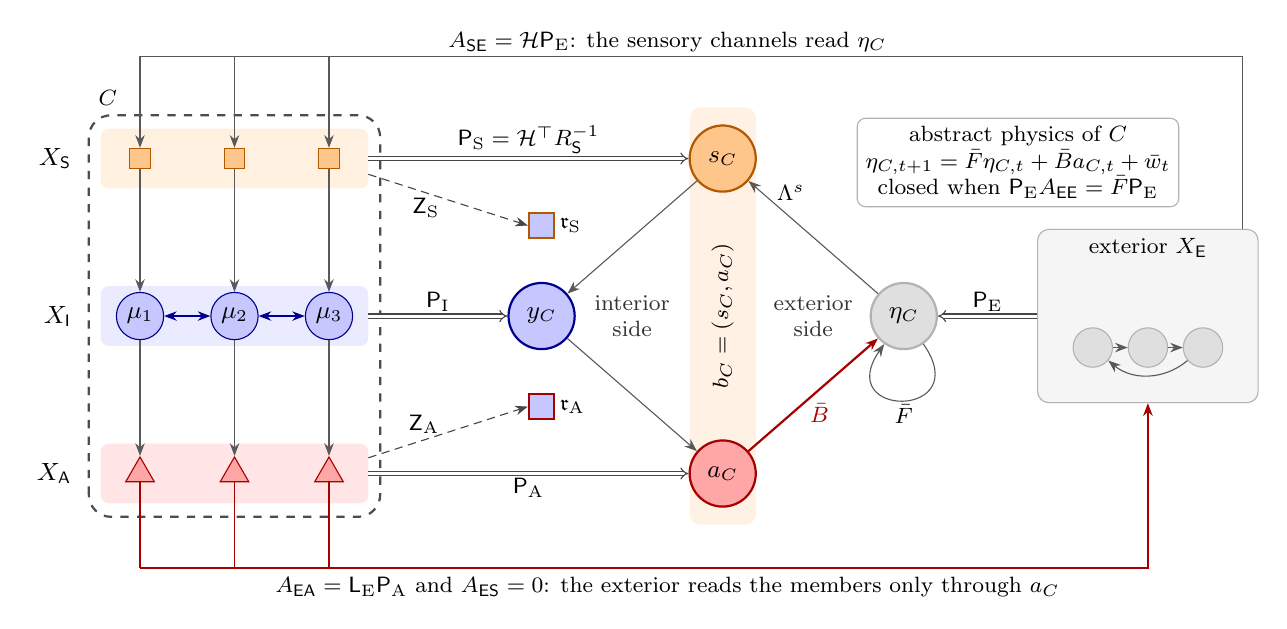
\begin{tikzpicture}[>={Stealth[length=1.6mm]}, every node/.style={font=\small},
    roleI/.style={fill=blue!22, draw=blue!55!black},
    roleS/.style={fill=orange!45, draw=orange!70!black},
    roleA/.style={fill=red!35, draw=red!65!black},
    roleE/.style={fill=gray!25, draw=gray!60},
    chan/.style={rectangle, minimum size=2.6mm, inner sep=0pt},
    outp/.style={regular polygon, regular polygon sides=3, minimum size=4.2mm, inner sep=0pt},
    intl/.style={circle, minimum size=6mm, inner sep=0pt},
    coarse/.style={circle, minimum size=8.4mm, inner sep=0pt, thick},
    resid/.style={rectangle, minimum size=3.2mm, inner sep=0pt, fill=blue!22, thick},
    map/.style={double, double distance=1.1pt, -Implies, gray!55!black},
    rmap/.style={->, gray!55!black, densely dashed},
    flow/.style={->, gray!70!black},
    act/.style={->, red!65!black, thick},
    lab/.style={font=\footnotesize, inner sep=1.5pt},
    mlab/.style={font=\footnotesize, inner sep=1.5pt, text=black}]
  % members of C: one column per member, one row per channel role
  \fill[orange!12, rounded corners=3pt] (0.8,6.62) rectangle (4.2,7.38);
  \fill[blue!8, rounded corners=3pt] (0.8,4.62) rectangle (4.2,5.38);
  \fill[red!10, rounded corners=3pt] (0.8,2.62) rectangle (4.2,3.38);
  \node[anchor=east] at (0.55,7.0) {$X_{\sS}$};
  \node[anchor=east] at (0.55,5.0) {$X_{\sI}$};
  \node[anchor=east] at (0.55,3.0) {$X_{\sA}$};
  \foreach \p/\x in {1/1.3, 2/2.5, 3/3.7} {
    \node[chan, roleS] (S\p) at (\x,7.0) {};
    \node[intl, roleI] (M\p) at (\x,5.0) {$\mu_{\p}$};
    \node[outp, roleA] (A\p) at (\x,3.0) {};
    \draw[flow] (S\p) -- (M\p);
    \draw[flow] (M\p) -- (A\p.north);
  }
  \draw[<->, blue!55!black] (M1) -- (M2);
  \draw[<->, blue!55!black] (M2) -- (M3);
  \draw[dashed, thick, black!70, rounded corners=8pt] (0.65,2.45) rectangle (4.35,7.55);
  \node[anchor=south west, font=\footnotesize] at (0.65,7.55) {$C$};
  % coarse states
  \fill[orange!10, rounded corners=4pt] (8.28,2.35) rectangle (9.12,7.65);
  \node[rotate=90, font=\footnotesize] at (8.7,5.0) {$b_C=(s_C,a_C)$};
  \node[coarse, roleI] (yC) at (6.4,5.0) {$y_C$};
  \node[coarse, roleS] (sC) at (8.7,7.0) {$s_C$};
  \node[coarse, roleA] (aC) at (8.7,3.0) {$a_C$};
  \node[coarse, roleE] (eC) at (11.0,5.0) {$\eta_C$};
  \node[resid, draw=orange!70!black] (rS) at (6.4,6.15) {};
  \node[resid, draw=red!65!black] (rA) at (6.4,3.85) {};
  \node[lab, anchor=west] at (rS.east) {$\mathfrak r_{\mathrm S}$};
  \node[lab, anchor=west] at (rA.east) {$\mathfrak r_{\mathrm A}$};
  \node[font=\footnotesize, align=center, gray!40!black] at (7.55,5.0) {interior\\side};
  \node[font=\footnotesize, align=center, gray!40!black] at (9.85,5.0) {exterior\\side};
  % coarse dynamics
  \draw[flow] (eC) -- node[mlab, above right=-1pt, pos=0.8] {$\Lambda^s$} (sC);
  \draw[flow] (sC) -- (yC);
  \draw[flow] (yC) -- (aC);
  \draw[act] (aC) -- node[lab, below right=-1pt, pos=0.45] {$\bar B$} (eC);
  \draw[flow] (eC) to[out=-55, in=-125, looseness=6] node[mlab, below] {$\bar F$} (eC);
  % exterior
  \node[draw=gray!60, fill=gray!8, rounded corners=4pt, minimum width=2.8cm, minimum height=2.2cm] (ext) at (14.1,5.0) {};
  \node[font=\footnotesize, anchor=north] at (ext.north) {exterior $X_{\sE}$};
  \foreach \k/\x in {1/13.4, 2/14.1, 3/14.8}
    \node[intl, roleE, minimum size=5mm] (E\k) at (\x,4.6) {};
  \draw[flow] (E1) -- (E2);
  \draw[flow] (E2) -- (E3);
  \draw[flow] (E3) to[bend left=40] (E1);
  % declared coarse maps
  \draw[map] (4.2,7.0) -- node[mlab, above] {$\mathsf P_{\mathrm S}=\mathcal H^\top R_{\sS}^{-1}$} (sC);
  \draw[map] (4.2,5.0) -- node[mlab, above] {$\mathsf P_{\mathrm I}$} (yC);
  \draw[map] (4.2,3.0) -- node[mlab, below] {$\mathsf P_{\mathrm A}$} (aC);
  \draw[map] (ext.west) -- node[mlab, above] {$\mathsf P_{\mathrm E}$} (eC);
  \draw[rmap] (4.2,6.8) -- node[mlab, below left=-2pt, pos=0.45] {$\mathsf Z_{\mathrm S}$} (rS.west);
  \draw[rmap] (4.2,3.2) -- node[mlab, above left=-2pt, pos=0.45] {$\mathsf Z_{\mathrm A}$} (rA.west);
  % abstract physics
  \node[draw=gray!60, fill=white, rounded corners=3pt, align=center, font=\footnotesize, inner sep=3pt] at (12.45,6.95)
    {abstract physics of $C$\\$\eta_{C,t+1}=\bar F\eta_{C,t}+\bar Ba_{C,t}+\bar w_t$\\closed when $\mathsf P_{\mathrm E}A_{\sE\sE}=\bar F\mathsf P_{\mathrm E}$};
  % fine couplings between the members and the exterior
  \draw[gray!70!black] (15.3,6.1) -- (15.3,8.3) -- (1.3,8.3);
  \foreach \p in {1,2,3} \draw[flow] (S\p.north |- 0,8.3) -- (S\p.north);
  \node[lab, anchor=south] at (8.0,8.3) {$A_{\sS\sE}=\mathcal H\mathsf P_{\mathrm E}$: the sensory channels read $\eta_C$};
  \foreach \p in {1,2,3} \draw[red!65!black, semithick] (A\p.south) -- (A\p.south |- 0,1.8);
  \draw[act] (1.3,1.8) -- (14.1,1.8) -- (ext.south);
  \node[lab, anchor=north] at (8.0,1.74) {$A_{\sE\sA}=\mathsf L_{\mathrm E}\mathsf P_{\mathrm A}$ and $A_{\sE\sS}=0$: the exterior reads the members only through $a_C$};
\end{tikzpicture}

  \caption{\textbf{A meta-agent as an agent.} Left: three members of $C$ (dashed box), each with a sensory channel (orange) that reads the exterior, an internal state $\mu_i$ (blue) that exchanges messages with the other members, and an active channel (red) that the exterior reads; the rows are the role groups $X_{\sS}$, $X_{\sI}$ and $X_{\sA}$ of the canonical partition, and the exterior $X_{\sE}$ is on the right. Declared linear maps of full row rank (double arrows) send these groups to the coarse states $y_C$, $s_C$, $a_C$ and $\eta_C$ of \eqref{eq:met-coarse}. The sensory map gives the information-form statistic $s_C=\mathcal H^\top R_{\sS}^{-1}X_{\sS}$, with information matrix $\Lambda^s=\mathcal H^\top R_{\sS}^{-1}\mathcal H$, and the residuals $\mathfrak r_{\mathrm S}=\mathsf Z_{\mathrm S}X_{\sS}$ and $\mathfrak r_{\mathrm A}=\mathsf Z_{\mathrm A}X_{\sA}$, which complete $\mathsf P_{\mathrm B}=\diag(\mathsf P_{\mathrm S},\mathsf P_{\mathrm A})$ to an invertible map, are assigned to the interior side (dashed arrows), so that the coarse blanket $b_C=(s_C,a_C)$ lies between the coarse interior and the coarse exterior. The sensory channels read the exterior only through $\eta_C$ and read no interior or active variable (top line), and the exterior reads the members only through the coarse act, $A_{\sE\sA}=\mathsf L_{\mathrm E}\mathsf P_{\mathrm A}$ and $A_{\sE\sS}=0$ (bottom line). With $\mathcal H$ of full column rank and memoryless channels these couplings satisfy conditions (a1) and (a2) of \cref{prop:met-sufficiency}, and from a start that satisfies (a3), $b_C$ is an exact strong coarse path blanket on every window. When in addition $\mathsf P_{\mathrm E}A_{\sE\sE}=\bar F\mathsf P_{\mathrm E}$, that is, when $\ker\mathsf P_{\mathrm E}$ is invariant under $A_{\sE\sE}$, the coarse exterior obeys the closed law $\eta_{C,t+1}=\bar F\eta_{C,t}+\bar Ba_{C,t}+\bar w_t$ given the coarse act, with $\bar B=\mathsf P_{\mathrm E}\mathsf L_{\mathrm E}$, the abstract physics of $C$ (\cref{thm:met-abstract-physics}).}
  \label{fig:met-partition}
\end{figure}

\begin{theorem}[Coarse path blankets]\label{thm:met-coarse-blanket}
Let $X$ follow \eqref{eq:col-joint} on $[0,T]$, $T\ge2$, from $X_0\sim\Ncal(\bar X_0,\Sigma_0)$ with $\Sigma_0\succ0$, independent of the noise, with the canonical partition of $C$ and noise independent across $(\sI,\sB,\sE)$.
\begin{enumerate}
\item[(a)] For a residual assignment, $X_{\sI',0:T}\perp X_{\sE',0:T}\mid b_{C,0:T}$ if and only if the general conditions of \cref{thm:col-path-blanket}(a) hold for $(\tilde A,\tilde Q,\mathcal S\Sigma_0\mathcal S^\top)$ and the partition $(\sI',\sB',\sE')$. If $\tilde Q$ is block diagonal for that partition, they read
\begin{equation}\label{eq:met-coarse-pb}
\tilde A_{\sI'\sE'}=0,\qquad\tilde A_{\sE'\sI'}=0,\qquad\tilde A_{\sB'\sI'}^\top\tilde Q_{\sB'\sB'}^{-1}\tilde A_{\sB'\sE'}=0,\qquad X_{\sI',0}\perp X_{\sE',0}\mid b_{C,0},
\end{equation}
and they imply the strong and the weak coarse path blankets.
\item[(b)] (Without an assignment.) Complete $\mathsf P_{\mathrm B}$ by any $\mathsf Z$ to an invertible map, put $\mathfrak r=\mathsf ZX_{\sB}$, and let $J$ be the precision of the path of $(X_{\sI},b_C,\mathfrak r,X_{\sE})$ on $[0,T]$. The strong coarse path blanket holds if and only if $J_{\sI\sE}-J_{\sI\mathfrak r}J_{\mathfrak r\mathfrak r}^{-1}J_{\mathfrak r\sE}=0$. Under the fine path blanket $J_{\sI\sE}=0$, and the condition is $J_{\sI\mathfrak r}J_{\mathfrak r\mathfrak r}^{-1}J_{\mathfrak r\sE}=0$. Let $J^{\mathrm b}$ be the precision of the paths of $(X_{\sI},X_{\sE})$ given $b_{C,0:T}$, the Schur complement of $J_{\mathfrak r\mathfrak r}$ in the block of $J$ that omits $b_C$, so that $J^{\mathrm b}_{\sI\sE}$ is the matrix above. The coarse leak is $\iota^C_T=-\frac12\ln\det(I-MM^\top)$ with $M=(J^{\mathrm b}_{\sI\sI})^{-1/2}J^{\mathrm b}_{\sI\sE}(J^{\mathrm b}_{\sE\sE})^{-1/2}$.
\end{enumerate}
\end{theorem}
% src: H3-T1; HC_critic V5
Proof in \cref{app:met}; checked in \cref{chk:met-blanket}. Part (b) is exact but not interpretable. The coarse blanket is related to the fine one in neither direction: \cref{ex:met-summary-leak} in the Supplement has a fine path blanket and a leaking coarse one, and in \cref{ex:col-collider}, where the fine blanket leaks, the coarse blanket with no coordinates separates the two independent outer variables. Whether every exact coarse blanket arises from a residual assignment that satisfies (a) is open. The next proposition gives interpretable sufficient conditions.

\begin{proposition}[Sufficient conditions for a coarse blanket]\label{prop:met-sufficiency}
In the setting of \cref{thm:met-coarse-blanket}, with per-channel noise:
\begin{enumerate}
\item[(a)] (The information-form statistic.) Assume the following.
\begin{enumerate}
\item[(a1)] The sensory channels read the exterior through a few coordinates, $A_{\sS\sE}=\mathcal H\mathsf G_{\mathrm E}$ with $\mathcal H$ of full column rank and $\mathsf G_{\mathrm E}$ of full row rank, both equal to the number of those coordinates; they read no interior or active variable, $A_{\sS\sI}=0$ and $A_{\sS\sA}=0$; and their memory is closed by the statistic: with $\mathsf P_{\mathrm S}=\mathcal H^\top R_{\sS}^{-1}$, $\mathsf P_{\mathrm S}A_{\sS\sS}=\mathcal C\mathsf P_{\mathrm S}$ for some $\mathcal C$, as for memoryless channels and for channels with equal memories.
\item[(a2)] The exterior reads the members only through the coarse act: $A_{\sE\sS}=0$ and $A_{\sE\sA}=\mathsf L_{\mathrm E}\mathsf P_{\mathrm A}$ for some matrix $\mathsf L_{\mathrm E}$.
\item[(a3)] $(X_{\sI},\mathfrak r_{\mathrm S},\mathfrak r_{\mathrm A})_0\perp X_{\sE,0}\mid b_{C,0}$, where $\mathfrak r_{\mathrm S}=\mathsf Z_{\mathrm S}X_{\sS}$ and $\mathfrak r_{\mathrm A}=\mathsf Z_{\mathrm A}X_{\sA}$, and the rows of $\mathsf Z_{\mathrm S}$ and $\mathsf Z_{\mathrm A}$ span $\{z:z\mathcal H=0\}$ and $\{z:zQ^{\Xi}_{\sA\sA}\mathsf P_{\mathrm A}^\top=0\}$.
\end{enumerate}
Then, with $s_C=\mathcal H^\top R_{\sS}^{-1}X_{\sS}$ and both residuals assigned to the interior, the strong coarse path blanket holds on every window, whatever the interior reads in the blanket and whatever the active channels read among collective variables. For memoryless channels the sensory residual is pure noise, independent of the exterior path and of $s_C$.
\item[(b)] (Closure of the blanket summary.) Let the noise be independent across $(\sI,\sB,\sE)$, and assume (b1) $A_{\sI\sB}=\mathcal B_{\sI}\mathsf P_{\mathrm B}$, (b2) $A_{\sE\sB}=\mathcal B_{\sE}\mathsf P_{\mathrm B}$ and (b3) $\mathsf P_{\mathrm B}A_{\sB\sB}=\mathcal A_{bb}\mathsf P_{\mathrm B}$ for some matrices $\mathcal B_{\sI},\mathcal B_{\sE},\mathcal A_{bb}$. Then $(X_{\sI},b_C,X_{\sE})$ is a linear-Gaussian Markov process whose path law is the marginal of that of $X$, and the strong coarse path blanket holds on $[0,T]$ if and only if (b4) $(\mathsf P_{\mathrm B}A_{\sB\sI})^\top(\mathsf P_{\mathrm B}Q^{\Xi}_{\sB\sB}\mathsf P_{\mathrm B}^\top)^{-1}\mathsf P_{\mathrm B}A_{\sB\sE}=0$ and (b5) $X_{\sI,0}\perp X_{\sE,0}\mid b_{C,0}$. Condition (b4) holds when $s_C$ reads no interior variable, $a_C$ reads no exterior variable and their noises are independent.
\item[(c)] (Ancillary residuals.) Under (a1), for a coarse sensory map $\mathsf P_{\mathrm S}$ and a complement $\mathsf Z$ with $\mathsf ZR_{\sS}\mathsf P_{\mathrm S}^\top=0$, the residual $\mathsf ZX_{\sS}$ reads no exterior variable if and only if $\operatorname{row}(\mathcal H^\top R_{\sS}^{-1})\subseteq\operatorname{row}(\mathsf P_{\mathrm S})$.
\end{enumerate}
\end{proposition}
% src: H3-P1, H3-P2; HC_critic V5 (scope)
Proof in \cref{app:met}; checked in \cref{chk:met-blanket}. Under (a), everything in the members' sensory channels other than the information-form statistic is noise that carries nothing about the exterior, so members may read their own channels without opening a leak, and by (c) an ancillary residual requires that statistic. The scope is set by (a1) and (a2): the exterior may not read the members' sensory channels, and no sensory channel may read an individual member's act (\cref{ex:met-reafference}), while a firm's act that reaches its sensors through the price, an exterior variable, is allowed. Reading the blanket through $s_C$ inside and through $a_C$ outside is not enough without (b3). \Cref{fig:met-partition} draws the coarse variables of a meta-agent with the residual assignment of \cref{prop:met-sufficiency}(a) and the closure condition of \cref{thm:met-abstract-physics}.

Three examples show how the sufficient conditions fail. In a model with two memoryless sensory channels and an exterior that is independent across rounds, an equal-weight summary leaks whenever the interior's gains on the two channels differ and the noise variances of the channels differ; sensory channels with unequal memories violate (a1) at the information-form statistic; and a collective sensor that reads one member's act violates (b3) (Supplement, \cref{ex:met-summary-leak,ex:met-channel-memory,ex:met-reafference}).

Small violations of the sufficient conditions leak at a rate quadratic in their size.

\begin{proposition}[Approximate coarse blankets]\label{prop:met-leak-bound}
For a residual assignment with $\tilde Q$ block diagonal for $(\sI',\sB',\sE')$ and a start with $(\tilde\Sigma_0^{-1})_{\sI'\sE'}=0$, where $\tilde\Sigma_0=\mathcal S\Sigma_0\mathcal S^\top$, abbreviate $\tilde Q_{\sI'\sI'}$ to $\tilde Q_{\sI'}$, and similarly, and put
\begin{equation}\label{eq:met-leak-blocks}
\mathsf D_{\mathrm c}=\tilde A_{\sI'\sI'}^\top\tilde Q_{\sI'}^{-1}\tilde A_{\sI'\sE'}+\tilde A_{\sB'\sI'}^\top\tilde Q_{\sB'}^{-1}\tilde A_{\sB'\sE'}+\tilde A_{\sE'\sI'}^\top\tilde Q_{\sE'}^{-1}\tilde A_{\sE'\sE'},\qquad\mathsf D_1=\tilde Q_{\sI'}^{-1}\tilde A_{\sI'\sE'},\qquad\mathsf D_2=\tilde Q_{\sE'}^{-1}\tilde A_{\sE'\sI'},
\end{equation}
$\mathsf k=\Vert\mathsf D_{\mathrm c}\Vert+\Vert\mathsf D_1\Vert+\Vert\mathsf D_2\Vert$ and $\mathsf k_F^2=\Vert\mathsf D_{\mathrm c}\Vert_F^2+\Vert\mathsf D_1\Vert_F^2+\Vert\mathsf D_2\Vert_F^2$. Assume $\rho(\tilde A_{\sI'\sI'})<1$ and $\rho(\tilde A_{\sE'\sE'})<1$, let $\mathfrak s_{\sI'}=\sum_{l\ge0}\Vert\tilde A_{\sI'\sI'}^l\Vert$ and $\mathfrak v_{\sI'}=\max\{\lambda_{\max}(\tilde\Sigma_0),\lambda_{\max}(\tilde Q_{\sI'})\}$, define $\mathfrak s_{\sE'}$ and $\mathfrak v_{\sE'}$ likewise, and put $\mathfrak c_C=(\mathfrak v_{\sI'}\mathfrak v_{\sE'})^{1/2}\mathfrak s_{\sI'}\mathfrak s_{\sE'}$. If $\mathfrak c_C\mathsf k<1$, then for every $T$
\begin{equation}\label{eq:met-leak-bound}
\iota^C_T\le I(X_{\sI',0:T};X_{\sE',0:T}\mid b_{C,0:T})\le\frac{T\mathfrak c_C^2\mathsf k_F^2}{2(1-\mathfrak c_C^2\mathsf k^2)}.
\end{equation}
The three blocks vanish under \eqref{eq:met-coarse-pb} and are linear in $\tilde A_{\sI'\sE'}$, $\tilde A_{\sE'\sI'}$ and the coarse collider term, so the bound on the leak rate is quadratic in the violation.
\end{proposition}
% src: H3-P3 (constants renamed per HC_critic 2.7: beta to k, beta_F to k_F, D to D_c; kappa_C to c_C)
Proof in \cref{app:met}. Perturbing the information-form weights of the three-member system of \cref{chk:met-blanket} by $\mathsf h(1,-1,0)$ gives leak rates proportional to $\mathsf h^2$, as the proposition predicts, but the constant $\mathfrak c_C=45.1$ makes the bound conservative by four orders of magnitude (\cref{chk:met-leak-bound}, \cref{open:met-leak-constant}).

\subsection{The abstract physics}\label{sec:met-physics}

No exterior variable reads an interior one, so the exterior evolves as $X_{\sE,t+1}=A_{\sE\sE}X_{\sE,t}+A_{\sE\sB}X_{\sB,t}+\Xi^{\sE}_t$, the recursion of \cref{def:agy-closure} with the blanket as input. Whether a declared coarse exterior obeys a law of its own given the coarse act is therefore the closure question of \cref{def:agy-closure} asked of the exterior.

\begin{definition}[Closure of coarse states and abstract physics]\label{def:met-abstract-physics}
Let $C$ have coarse variables as in \cref{def:met-coarse}.
\begin{enumerate}
\item[(i)] (Interior.) The coarse internal state is exactly closed given $b_C$ when $\mathsf P_{\mathrm I}A_{\sI\sI}=\bar A_y\mathsf P_{\mathrm I}$ and $\mathsf P_{\mathrm I}A_{\sI\sB}=\bar B_y\mathsf P_{\mathrm B}$ for some $\bar A_y,\bar B_y$, so that $y_{C,t+1}=\bar A_yy_{C,t}+\bar B_yb_{C,t}+\mathsf P_{\mathrm I}\Xi^{\sI}_t$. In the stationary process its closure defect is $\mathfrak d^C_{\mathrm{cl}}=I(y_{C,t+1};X_{\sI,t},X_{\sB,t}\mid y_{C,t},b_{C,t})$.
\item[(ii)] (Exterior.) The coarse exterior has an exact abstract physics given $a_C$ when $\mathsf P_{\mathrm E}A_{\sE\sE}=\bar F\mathsf P_{\mathrm E}$, $\mathsf P_{\mathrm E}A_{\sE\sS}=0$ and $\mathsf P_{\mathrm E}A_{\sE\sA}=\bar B\mathsf P_{\mathrm A}$ for some $\bar F,\bar B$, so that
\begin{equation}\label{eq:met-abstract-physics}
\eta_{C,t+1}=\bar F\eta_{C,t}+\bar Ba_{C,t}+\bar w_t,\qquad\bar w_t=\mathsf P_{\mathrm E}\Xi^{\sE}_t\sim\Ncal(0,\bar Q),\qquad\bar Q=\mathsf P_{\mathrm E}Q^{\Xi}_{\sE\sE}\mathsf P_{\mathrm E}^\top,
\end{equation}
with $\bar w_t$ independent of $X_{0:t}$. In the stationary process its closure defect and its relative predictive defect for each coordinate $\alpha$ of $\eta_C$ are
\begin{equation}\label{eq:met-exterior-defects}
\mathfrak d^{\mathrm E}_{\mathrm{cl}}=I\bigl(\eta_{C,t+1};X_{\sE,t},X_{\sB,t}\bigm|\eta_{C,t},a_{C,t}\bigr),\qquad\mathfrak e^{\mathrm E}_\alpha=\frac{\E\bigl(\E[\eta_{C,t+1,\alpha}\mid X_t]-\E[\eta_{C,t+1,\alpha}\mid\eta_{C,t},a_{C,t}]\bigr)^2}{\Var(\eta_{C,t+1,\alpha})}.
\end{equation}
\item[(iii)] (Vocabulary.) A coarse variable is exactly closed when its map satisfies the conditions of (i) or (ii), which are kernel-invariance conditions (\cref{thm:met-abstract-physics}(c)). It is closed of order $d$ when it becomes exactly closed after $d$ linear functionals of the hidden coordinates are adjoined to it, the least such $d$ being its minimal order $d^\ast$; this order counts hidden coordinates and bounds from above the closure order $\mathrm{ord}(\alpha_{\mathrm M})$ of \cref{def:agy-closure}(iii), which counts functionals of the filter state and can be smaller (see the discussion after \cref{thm:met-abstract-physics}). It is approximately closed when a stated memory measure, a defect of (i) or (ii), a Markov error or the weight of the memory kernels of \cref{thm:agy-mori-zwanzig}, lies below a stated bound. The abstract physics of a meta-agent is the exactly or approximately closed law of its coarse exterior given its coarse act; whether a meta-agent has one is decided by \cref{thm:met-abstract-physics,prop:met-memory}, never assumed.
\end{enumerate}
\end{definition}
% src: H3-D3, H3-D4, decision 19, HC_critic 2.2

The relative predictive defect measures memory against the variance of the coarse exterior rather than against its own noise, which matters for aggregates (\cref{rem:met-aggregate-defect}). An exterior that reads the members only through the coarse act is closed of order at most $\dim X_{\sE}-\dim\eta_C$, so a closure claim for a finite population has content only through its order or its memory bound.

\begin{definition}[Lumpable partition]\label{def:met-lumpable}
Let $A$ be a square matrix indexed receiver first, so that $A_{uv}$ is the weight that $u$ places on $v$, and let $\{\mathfrak B_\alpha\}$ be a partition of its index set. The partition is lumpable for $A$ when, for every pair of blocks $\alpha,\beta$, the total weight that the receivers of block $\alpha$ place on sender $v$,
\begin{equation}\label{eq:met-lumpable}
\sum_{u\in\mathfrak B_\alpha}A_{uv},
\end{equation}
is the same for every $v\in\mathfrak B_\beta$. The common value $\bar A_{\alpha\beta}$ is the coarse weight; equivalently, the block-sum matrix satisfies $\mathsf PA=\bar A\mathsf P$.
\end{definition}
% src: H3-T2(e), H4-T18(2), H5-P5(b), unified per HC_critic V6

For one block it is equality of the column sums of $A$ (\cref{prop:met-level0,prop:env-aggregate-closure}); for a Markov chain with transition matrix $A^\top$ it is lumpability in the sense of \citet{kemeny1960finite}.

\begin{theorem}[Exact abstract physics]\label{thm:met-abstract-physics}
Let $\eta_C=\mathsf P_{\mathrm E}X_{\sE}$ and $a_C=\mathsf P_{\mathrm A}X_{\sA}$ be of full row rank, and let $\mathcal O$ be the observability matrix of $(\mathsf P_{\mathrm E},A_{\sE\sE})$, with block rows $\mathsf P_{\mathrm E}A_{\sE\sE}^l$, $0\le l<\dim X_{\sE}$. The following are equivalent.
\begin{enumerate}
\item[(a)] (Algebraic.) $\mathsf P_{\mathrm E}A_{\sE\sE}=\bar F\mathsf P_{\mathrm E}$, $\mathsf P_{\mathrm E}A_{\sE\sS}=0$ and $\mathsf P_{\mathrm E}A_{\sE\sA}=\bar B\mathsf P_{\mathrm A}$ for some $\bar F,\bar B$.
\item[(b)] (Dynamical.) For every initial law, \eqref{eq:met-abstract-physics} holds at every round; equivalently, in the representation of $\eta_C$ by \cref{thm:agy-mori-zwanzig} with the blanket as input, the memory kernels, the initial-state term and the colored noise vanish and the input term is a function of $a_C$.
\item[(c)] (Kernel invariance.) $\ker\mathsf P_{\mathrm E}$ is invariant under $A_{\sE\sE}$, equivalently $\rank\mathcal O=\rank\mathsf P_{\mathrm E}$, and $\mathsf P_{\mathrm E}A_{\sE\sS}=0$ and $\mathsf P_{\mathrm E}A_{\sE\sA}$ vanishes on $\ker\mathsf P_{\mathrm A}$.
\item[(d)] (Stationary, when $\rho(A)<1$.) $\mathfrak d^{\mathrm E}_{\mathrm{cl}}=0$.
\end{enumerate}
In addition:
\begin{enumerate}
\item[(e)] (Block sums.) If $\mathsf P_{\mathrm E}$ is the block-sum matrix of a partition of the exterior coordinates, the first condition of (a) holds if and only if the partition is lumpable for $A_{\sE\sE}$ (\cref{def:met-lumpable}), and then $\bar F$ is the matrix of coarse weights.
\item[(f)] (Minimal closed extension.) The row space $\mathcal R^\ast=\operatorname{row}\mathcal O$ is the smallest space of row vectors that contains $\operatorname{row}\mathsf P_{\mathrm E}$ and is invariant under right multiplication by $A_{\sE\sE}$, and every coarse exterior $\mathsf P^\ast X_{\sE}$ that contains $\eta_C$ and satisfies the first condition of (a) has $\operatorname{row}\mathsf P^\ast\supseteq\mathcal R^\ast$. A coarse exterior with row space $\mathcal R^\ast$ satisfies the first condition of (a); it has an exact abstract physics given $a_C$ if and only if $\mathsf P^\ast A_{\sE\sS}=0$ and $\mathsf P^\ast A_{\sE\sA}$ vanishes on $\ker\mathsf P_{\mathrm A}$, and if it has none, no coarse exterior containing $\eta_C$ has one. When it has one, the minimal order of $\eta_C$ is $d^\ast=\rank\mathcal O-\rank\mathsf P_{\mathrm E}$, the observability rank of the memory system of \cref{thm:agy-mori-zwanzig} for $\eta_C$, and $\ker\mathcal O$ is the largest $A_{\sE\sE}$-invariant subspace of $\ker\mathsf P_{\mathrm E}$.
\end{enumerate}
\end{theorem}
% src: H3-T2; HC_critic V6; decision 19 (minimal order)
Proof in \cref{app:met}; checked in \cref{chk:met-physics}. Every declared coarse exterior thus has a unique smallest closed completion, made of $\eta_C$ and the part of the hidden exterior that $\eta_C$ eventually feels; a meta-agent that models only $\eta_C$ with a Markov law is misspecified unless $d^\ast=0$, and \cref{ex:met-two-firms} computes the cost. The hidden filter of \cref{thm:agy-closure-identity}(d) is another completion, closed in law, and its least order at tolerance zero is the closure order $\mathrm{ord}(0)$ of \cref{def:agy-closure}(iii). The two orders differ in kind: $d^\ast$ counts linear functionals of the hidden coordinates and asks for a closed equation of motion, whereas $\mathrm{ord}(\alpha_{\mathrm M})$ counts linear functionals of the filter state and asks for a Markov law of the observed path within the tolerance $\alpha_{\mathrm M}$. They are related by $\mathrm{ord}(\alpha_{\mathrm M})\le\mathrm{ord}(0)\le\rank\mathcal O-\rank\mathsf P_{\mathrm E}$: the coordinates adjoined in $\mathcal R^\ast$ may be taken as functionals of the hidden coordinates, their conditional mean given the path of $\eta_C$ and the input path is the same functional of the filter state, and that mean together with $\eta_C$ is a Markov state for the law of $\eta_C$ given the input path. The second inequality can be strict. For $\eta_{t+1}=\frac14\eta_t+\sqrt{7/8}z_t+\mathfrak n_t$ and $z_{t+1}=\frac12z_t+\mathfrak n'_t$ with independent noises of unit variance, the stationary $\eta$ is a first-order autoregression with coefficient $\frac12$ and innovation variance $2$, so that $\mathrm{ord}(0)=0$ while $\rank\mathcal O-\rank\mathsf P_{\mathrm E}=1$ (\cref{chk:met-orders}). The value of $\mathrm{ord}(0)$ in general, a problem of minimal stochastic realization, is open (\cref{sec:agy}). Renormalization and aggregation use part (e) (\cref{thm:ren-closure,prop:env-aggregate-closure}). \Citet{rosas2024software} characterize closed levels of stationary processes without an environment through lumpability of causal states; the theorem is a linear-Gaussian, input-driven and one-step counterpart (\cref{prop:met-closure-notions}).

When the exterior is not exactly closed, its memory is bounded by the coupling between $\eta_C$ and the hidden exterior and by a timescale ratio of the exterior.

\begin{proposition}[Approximate abstract physics]\label{prop:met-memory}
In the setting of \cref{thm:met-abstract-physics}, write the exterior in Mori coordinates $(\eta_C,x_\perp)$ with blocks $A_{yy},A_{y\perp},A_{\perp y},A_{\perp\perp}$ of $A_{\sE\sE}$ and input blocks $B_y=\mathsf P_{\mathrm E}A_{\sE\sB}$ and $B_\perp$, as in \cref{thm:agy-mori-zwanzig}.
\begin{enumerate}
\item[(a)] (Memory kernels.) If $\Vert A_{\perp\perp}^l\Vert\le M_\perp\alpha_\perp^l$ with $\alpha_\perp<1$, the kernels of \cref{thm:agy-mori-zwanzig} obey
\[
\Vert\Gamma_l\Vert\le M_\perp\Vert A_{y\perp}\Vert\Vert A_{\perp y}\Vert\alpha_\perp^{l-1},\qquad\Vert\Gamma^{\sB}_l\Vert\le M_\perp\Vert A_{y\perp}\Vert\Vert B_\perp\Vert\alpha_\perp^{l-1},
\]
and their total weights over $l\ge1$ are at most the same expressions with $\alpha_\perp^{l-1}$ replaced by $(1-\alpha_\perp)^{-1}$.
\item[(b)] (Defects.) Let $x=(X_{\sE,t},X_{\sB,t})$, $\mathsf G=\mathsf P_{\mathrm E}(A_{\sE\sE}\ A_{\sE\sB})$, $\mathsf c=(\eta_{C,t},a_{C,t})$, and let $\Sigma_{x\mid\mathsf c}$ be the stationary conditional covariance of $x$ given $\mathsf c$. Then $\mathfrak d^{\mathrm E}_{\mathrm{cl}}=\frac12\ln\det(I+\bar Q^{-1}\mathsf G\Sigma_{x\mid\mathsf c}\mathsf G^\top)\le\frac12\tr(\bar Q^{-1}\mathsf G\Sigma_{x\mid\mathsf c}\mathsf G^\top)$ and $\mathfrak e^{\mathrm E}_\alpha=(\mathsf G\Sigma_{x\mid\mathsf c}\mathsf G^\top)_{\alpha\alpha}/\Var(\eta_{C,\alpha})$; both vanish under \cref{thm:met-abstract-physics}(a).
\item[(c)] (One coordinate, continuous time.) Let the exterior obey $\mathrm dX_{\sE}=-M_{\sE}X_{\sE}\mathrm dt+\sqrt2\mathrm d\mathsf B_t$ with the input held fixed and $M_{\sE}+M_{\sE}^\top\succ0$, let $\eta_C=\phi^\top X_{\sE}$ with $\lvert\phi\rvert=1$, let $r_\phi=\xin^M/\xout^M>1$ be the drift-based contrast of the coordinate, with the rates of \cref{lem:met-unit-coordinate}(a), and let $\hat\sigma=\max(\sigma_{\mathrm{row}},\sigma_{\mathrm{col}})/\xout^M$. For symmetric $M_{\sE}$, $\Xi\le\hat\sigma^2/(r_\phi(r_\phi-1)^2)$. For general $M_{\sE}$, $\Xi\le304\hat\sigma^2/(r_\phi(r_\phi-1)^2)$ whenever $\hat\sigma\le(r_\phi-1)/4$ and $\hat\sigma^2\le(r_\phi-1)/2$.
\item[(d)] (One coordinate, discrete time.) For a reversible exterior with spectrum in $[0,1)$ and the input held fixed, $\eta_C=f^\top X_{\sE}$, the drift-based discrete contrast $r^{\mathrm d}=\xin^{\mathrm d}/\xout^{\mathrm d}>1$ and $\mathsf s=\sigma^{\mathrm d}/\xout^{\mathrm d}$ of \cref{lem:met-discrete-closure}(a), $\Xi^{\mathrm d}\le2\mathsf s^2/(r^{\mathrm d}(r^{\mathrm d}-1)^2)$.
\end{enumerate}
\end{proposition}
% src: H3-P4, sharpened through the merged lemmas (HC_critic V2, V10); constant 304 from thm:agy-closure-average(b)(iii)
Proof in \cref{app:met}. At fixed relative dispersion the bound on the memory of a coordinate falls like the inverse cube of its drift-based contrast, which compares the slowest relaxation of the hidden exterior with that of the abstract variable. For a reversible continuous-time exterior the drift is the stationary precision. When the exterior is a single region $C'$ with everything outside it held fixed and $\eta_C$ is its average in the unit-norm normalization, the outward rate is $\xout(C')$ of \cref{def:col-contrast} and the inward rate lies between $\xin(C')$ and $\xin(C')+\max_{i\in C'}a^\partial_i$, because the drift keeps the cut couplings on the diagonal, so the drift-based contrast is at least $r(C')$ and exceeds it in general with no circulation at all. When the exterior is larger than the region, the inward rate is a minimum over every direction of the exterior orthogonal to the average, the slow modes outside the region included, and can fall below $\xin(C')$. For non-reversible drift the rates differ in addition by a term set by the stationary current (\cref{prop:agy-drift-precision}).

For an exterior made of a price and $N\ge2$ outside traders, with the price and the traders' average as coarse exterior, the abstract physics is exact if and only if the traders' persistences are all equal; in general the stationary average obeys an exact equation with a memory kernel whose weight need not vanish as $N$ grows, while the variance of its colored noise is $O(1/N)$ (Supplement, \cref{ex:met-traders}). The consequence for the information-form defect of aggregates is in \cref{rem:met-aggregate-defect}.

In an example where the exterior contains a ring $C'$ of eight other agents with symmetric update and $\eta_C$ is the average of $C'$, the Markov error of the free dynamics of $\eta_C$ falls from $7.8\times10^{-3}$ to $8.1\times10^{-6}$ as the drift-based discrete contrast of $C'$ (\cref{lem:met-discrete-closure}) rises from $1.06$ to $10.04$ (Supplement, \cref{ex:met-other-collectives}). That contrast is computed from the drift of $C'$ with $C$'s act held fixed; it is not the precision-based contrast of \cref{def:col-contrast}, which selects collectives.

\subsection{Closure lemmas}\label{sec:met-lemmas}

The memory bounds above extend \cref{thm:agy-closure-average} to arbitrary coordinates and to discrete time. For a symmetric matrix $\mathsf M$, a unit vector $\phi$ and a matrix $Z$ whose rows are an orthonormal basis of $\phi^\perp$, write
\begin{equation}\label{eq:met-rates}
\xout(\mathsf M,\phi)=\phi^\top\mathsf M\phi,\qquad\xin(\mathsf M,\phi)=\lambda_{\min}(Z\mathsf MZ^\top),\qquad\sigma(\mathsf M,\phi)=\lvert Z\mathsf M\phi\rvert=\bigl\lvert(\mathsf M-\xout(\mathsf M,\phi))\phi\bigr\rvert,
\end{equation}
the rates and the dispersion of \cref{thm:agy-closure-average} with $\phi_C$ replaced by $\phi$. For the block $\Pi_{CC}$ of a diffusive precision and $\phi=\phi_C$, $\xout(\Pi_{CC},\phi_C)=\xout(C)$, $\sigma(\Pi_{CC},\phi_C)=\sigma_C$, and $\xin(\Pi_{CC},\phi_C)\ge\xin(C)$ because the cut couplings stay on the diagonal.

\begin{lemma}[Closure bounds for any coordinate]\label{lem:met-unit-coordinate}
\begin{enumerate}
\item[(a)] \Cref{thm:agy-closure-average} holds with $\phi_C$ replaced by any unit vector $\phi$ and $Z$ by an orthonormal basis of $\phi^\perp$: in part (b) with $\xout^M=\phi^\top M\phi$, $\xin^M=\lambda_{\min}(ZM_{\mathrm{sym}}Z^\top)$, $\sigma_{\mathrm{row}}=\lvert ZM\phi\rvert$ and $\sigma_{\mathrm{col}}=\lvert ZM^\top\phi\rvert$, and in part (a), for symmetric positive definite $M$, with $\xout$, $\xin$ and $\sigma_C$ replaced by the rates \eqref{eq:met-rates} of $(M,\phi)$. The readings of these quantities through row and column sums, leaks and attention hold for $\phi_C$ only.
\item[(b)] Let $M$ be symmetric positive definite with $\xin(M,\phi)>\xout(M,\phi)$. Then the smallest eigenvalue $\varpi_1$ of $M$ is simple, its eigenvector $\mathsf u_1$ satisfies $\tan\angle(\phi,\mathsf u_1)\le\sigma(M,\phi)/(\xin(M,\phi)-\xout(M,\phi))$, and the Markov error of $y=\phi^\top x$ in the stationary process $\mathrm dx=-Mx\mathrm dt+\sqrt2\mathrm d\mathsf B_t$ satisfies
\begin{equation}\label{eq:met-unit-markov}
\Xi\le\Bigl(\frac{\sigma(M,\phi)}{\xin(M,\phi)-\xout(M,\phi)}\Bigr)^2\frac{\xout(M,\phi)}{\xin(M,\phi)},
\end{equation}
with no condition on $\sigma(M,\phi)$. For $M=\Pi_{CC}$ and $\phi=\phi_C$, where $\xin(\Pi_{CC},\phi_C)\ge\xin(C)$, the right-hand side is, under the hypothesis $\xin(C)>\xout(C)$ of \cref{thm:agy-closure-average}(a), at most that of \eqref{eq:agy-markov-sym}, which likewise carries no condition on $\sigma_C$.
\end{enumerate}
\end{lemma}
% src: H3-L3 (written proof as required by HC_critic Section 3), HC_critic V2 (tangent bound and sharper Markov bound)
Proof in \cref{app:met}; checked in \cref{chk:met-lemmas}.

\begin{lemma}[Discrete-time closure of one coordinate]\label{lem:met-discrete-closure}
Let $x_{t+1}=Ax_t+\mathfrak n_t$ with $\mathfrak n_t\sim\Ncal(0,Q^{\mathfrak n})$, $Q^{\mathfrak n}\succ0$, independent across rounds, be reversible, $AQ^{\mathfrak n}=Q^{\mathfrak n}A^\top$, and let $y=f^\top x$ with $f\neq0$. Put $\tilde A=(Q^{\mathfrak n})^{-1/2}A(Q^{\mathfrak n})^{1/2}$, which is symmetric, and $\phi=(Q^{\mathfrak n})^{1/2}f/\lvert(Q^{\mathfrak n})^{1/2}f\rvert$; let $\varpi_1\le\varpi_2\le\dots$ be the eigenvalues of $I-\tilde A$, $\mathsf u_1$ an eigenvector of $\varpi_1$, and, in the stationary process, $\Xi^{\mathrm d}=\sup_{u\in\mathbb N}\lvert\Corr(y_t,y_{t+u})-(1-\varpi_1)^u\rvert$.
\begin{enumerate}
\item[(a)] (Drift rates.) Let the spectrum of $A$ lie in $[0,1)$, let $\xout^{\mathrm d}$, $\xin^{\mathrm d}$ and $\sigma^{\mathrm d}$ be the rates \eqref{eq:met-rates} of $(I-\tilde A,\phi)$, and let $\xin^{\mathrm d}>\xout^{\mathrm d}$. Then $\varpi_1$ is simple, $\xout^{\mathrm d}-(\sigma^{\mathrm d})^2/(\xin^{\mathrm d}-\xout^{\mathrm d})\le\varpi_1\le\xout^{\mathrm d}$, $\tan\angle(\phi,\mathsf u_1)\le\sigma^{\mathrm d}/(\xin^{\mathrm d}-\xout^{\mathrm d})$, and
\begin{equation}\label{eq:met-discrete}
\Xi^{\mathrm d}\le\tan^2\angle(\phi,\mathsf u_1)\frac{\varpi_1(2-\varpi_1)}{\varpi_2(2-\varpi_2)}\le\Bigl(\frac{\sigma^{\mathrm d}}{\xin^{\mathrm d}-\xout^{\mathrm d}}\Bigr)^2\frac{\xout^{\mathrm d}(2-\xout^{\mathrm d})}{\xin^{\mathrm d}(2-\xin^{\mathrm d})}\le2\Bigl(\frac{\sigma^{\mathrm d}}{\xin^{\mathrm d}-\xout^{\mathrm d}}\Bigr)^2\frac{\xout^{\mathrm d}}{\xin^{\mathrm d}}.
\end{equation}
\item[(b)] (Precision rates.) Under the same spectral condition, let $\xout^\Pi$, $\xin^\Pi$ and $\sigma^\Pi$ be the rates of $(I-\tilde A^2,\phi)$, where $I-\tilde A^2=(Q^{\mathfrak n})^{1/2}\Pi(Q^{\mathfrak n})^{1/2}$ is the whitened stationary precision of $x$. If $\xin^\Pi>\xout^\Pi$, then $\tan\angle(\phi,\mathsf u_1)\le\sigma^\Pi/(\xin^\Pi-\xout^\Pi)$ and $\Xi^{\mathrm d}\le(\sigma^\Pi/(\xin^\Pi-\xout^\Pi))^2\xout^\Pi/\xin^\Pi$.
\item[(c)] (Mixed signs.) If the spectrum of $A$ lies in $(-1,1)$ and its largest eigenvalue is $\rho(A)$, then under $\xin^{\mathrm d}>\xout^{\mathrm d}$ the tangent bound of (a) holds and $\Xi^{\mathrm d}\le2\tan^2\angle(\phi,\mathsf u_1)(1-\rho(A)^2)/(1-\max_{l\ge2}(1-\varpi_l)^2)$.
\end{enumerate}
For a level-0 collective with the exterior held fixed, symmetric $W_{CC}$ with spectrum in $[0,1)$ and $Q^\zeta_{CC}=qI$, (a) applies with $A=W_{CC}$ and $\phi=\phi_C$; then $\xout^{\mathrm d}$ and $\sigma^{\mathrm d}$ are the mean and the root-mean-square dispersion of the members' total leaks $1-\sum_{j\in C}W_{ij}$, and $\xin^{\mathrm d}/\xout^{\mathrm d}$ is the drift-based discrete contrast of $C$.
\end{lemma}
% src: H3-L2 merged with H4-P10 (HC_critic V10, 2.6): tangent bound without sigma < gap; part (b) added here and checked
Proof in \cref{app:met}; checked in \cref{chk:met-lemmas}, including recursions with $\sigma^{\mathrm d}\ge\xin^{\mathrm d}-\xout^{\mathrm d}$. Part (b) uses the stationary precision of the members with the exterior held fixed, which differs from the block of the population's world-conditional precision on which contrast is defined, so the lemma settles the reversible case of \cref{open:agy-discrete-closure} for one coordinate, and that problem remains open for the precision-based contrast of \cref{def:col-contrast} and for non-reversible recursions.

The closure notions in use are related exactly: in the stationary case without input, kernel invariance, a vanishing closure defect, vanishing dynamical dependence at every $t\ge1$ and one-step informational closure coincide, and of their approximate forms the closure defect is the largest (Supplement, \cref{prop:met-closure-notions}).

\subsection{The meta-agent's inference}\label{sec:met-inference}

The coarse generative model of $C$ is the linear-Gaussian state-space model with state $\eta_C$, dynamics $(\bar F,\bar B,\bar Q)$ of \eqref{eq:met-abstract-physics} with $a_C$ as a known input, and observation $s_{C,t+1}=\Lambda^s\eta_{C,t}+\bar v_t$, $\bar v_t\sim\Ncal(0,\Lambda^s)$, the law of the information-form statistic of memoryless readers of $\eta_C$. Let $\mathcal F_t$ be generated by the meta-agent's initial information $\mathcal I_0$ and by $(s_{C,1:t},a_{C,0:t})$. Because $s_{C,t}$ reads $\eta_{C,t-1}$, the one-round latency of \eqref{eq:col-joint}, the law of $\eta_{C,t}$ given $\mathcal F_t$ is the meta-agent's predictive law of the current exterior.

\begin{proposition}[Consensus on contributions gives the coarse filter]\label{prop:met-consensus-filter}
Assume the following.
\begin{enumerate}
\item[(S)] The exterior-facing sensory channels are memoryless readers of $\eta_C$, $X_{\sS,t+1}=\mathcal H\eta_{C,t}+\Xi^{\sS}_t$ with $R_{\sS}$ block diagonal over channels and $\mathcal H=\mathcal H_0\mathsf G_\eta$, $\mathcal H_0$ of full column rank and $\mathsf G_\eta$ of full row rank ($\mathsf G_\eta=I$ when every coordinate of $\eta_C$ is sensed), and read no interior or active variable. Condition (a1) of \cref{prop:met-sufficiency} then holds with $\mathcal H_0$ for $\mathcal H$ and $\mathsf G_{\mathrm E}=\mathsf G_\eta\mathsf P_{\mathrm E}$, and $s_C=\mathcal H^\top R_{\sS}^{-1}X_{\sS}$, the image of the statistic $\mathcal H_0^\top R_{\sS}^{-1}X_{\sS}$ of that proposition under the injective map $\mathsf G_\eta^\top$, satisfies $s_{C,t+1}=\Lambda^s\eta_{C,t}+\bar v_t$ with $\Lambda^s=\mathcal H^\top R_{\sS}^{-1}\mathcal H\succeq0$ and $\bar v_t\sim\Ncal(0,\Lambda^s)$, a Gaussian law that is degenerate when $\Lambda^s$ is singular. When $\mathsf G_\eta\ne I$ the map $\mathcal H^\top R_{\sS}^{-1}=\mathsf G_\eta^\top\mathcal H_0^\top R_{\sS}^{-1}$ is not of full row rank; the coarse sensory state in the sense of \cref{def:met-coarse} is then $s^0_C=\mathcal H_0^\top R_{\sS}^{-1}X_{\sS}$, whose map has full row rank, and $s_C=\mathsf G_\eta^\top s^0_C$ is its image under an injective linear map, so the two generate the same conditioning and the coarse blanket, the leaks and the closure defects computed with either coincide.
\item[(X)] The coarse exterior has an exact abstract physics with $\bar Q\succ0$, and the exterior reads the members only through $a_C$, condition (a2) of \cref{prop:met-sufficiency}.
\item[(Ind)] Conditionally on $\mathcal I_0$, $\eta_{C,0}\sim\Ncal(\hat\eta^-_0,P^-_0)$, independent of the initial collective variables.
\end{enumerate}
Then:
\begin{enumerate}
\item[(a)] For every $t$, $\eta_{C,t}\mid\mathcal F_t\sim\Ncal(\hat\eta^-_t,P^-_t)$, computed by the Kalman filter of the coarse generative model with $a_C$ as a known input,
\begin{equation}\label{eq:met-filter}
\begin{gathered}
\hat\eta^{\mathrm f}_{t-1}=\hat\eta^-_{t-1}+P^{\mathrm f}_{t-1}\bigl(s_{C,t}-\Lambda^s\hat\eta^-_{t-1}\bigr),\qquad(P^{\mathrm f}_{t-1})^{-1}=(P^-_{t-1})^{-1}+\Lambda^s,\\
\hat\eta^-_t=\bar F\hat\eta^{\mathrm f}_{t-1}+\bar Ba_{C,t-1},\qquad P^-_t=\bar FP^{\mathrm f}_{t-1}\bar F^\top+\bar Q,
\end{gathered}
\end{equation}
and conditioning in addition on the paths of all members' sensory channels and internal states leaves this law unchanged: the coarse blanket is sufficient for the meta-agent's inference.
\item[(b)] (Implementation by members.) Let member $i$ own the channels $X_{\sS_i}$, with blocks $\mathcal H_i$ and $R_{\sS,i}$ and contribution $h^s_i(t)=\mathcal H_i^\top R_{\sS,i}^{-1}X_{\sS_i,t}$, so that $s_{C,t}=\sum_ih^s_i(t)$. Let the pair $(\bar F,\Lambda^s)$ be detectable, that is, $\rho(\bar F-\mathsf L\Lambda^s)<1$ for some matrix $\mathsf L$, as when $\rho(\bar F)<1$ or $\Lambda^s\succ0$, so that the steady-state covariances exist (\cref{lem:met-riccati}). Let the members run $n_{\mathrm c}\ge0$ rounds of consensus with a matrix $\mathcal W$ that preserves sums, $\one^\top\mathcal W=\one^\top$, giving $\tilde h(t)=(\mathcal W^{n_{\mathrm c}}\otimes I)h^s(t)$, followed by
\begin{equation}\label{eq:met-member-filter}
\hat\eta^{(i)}_t=\bar F\bigl[\hat\eta^{(i)}_{t-1}+\bar P\bigl(n\tilde h_i(t)-\Lambda^s\hat\eta^{(i)}_{t-1}\bigr)\bigr]+\bar Ba_{C,t-1},
\end{equation}
with the steady-state filtered and predicted covariances $\bar P$ and $\bar P^-$ of \eqref{eq:met-filter}. Then the average $y_{C,t}=n^{-1}\sum_i\hat\eta^{(i)}_t$ obeys the steady-state form of \eqref{eq:met-filter} pathwise, for every $n_{\mathrm c}\ge0$; from the centralized start it equals $\hat\eta^-_t$ when $P^-_0=\bar P^-$. The deviations $\mathrm{dev}_i=\hat\eta^{(i)}-y_C$ obey $\mathrm{dev}_i(t)=\bar F(I-\bar P\Lambda^s)\mathrm{dev}_i(t-1)+n\bar F\bar P(\tilde h_i(t)-\bar h^s(t))$, and for symmetric, doubly stochastic and nonnegative $\mathcal W$ they obey a bound of the form of \cref{prop:agy-consensus}(b), with the factor $\rho_\perp^{n_{\mathrm c}}$.
\item[(c)] Every member's belief $\Ncal(\hat\eta^{(i)}_t,\bar P^-)$ is a translate of one Gaussian law.
\end{enumerate}
\end{proposition}
% src: H3-P5, H3-D5; HC_critic V7(a) (predictive law, one-round latency); number of rounds renamed n_{\mathrm c} (HC_critic 2.7)
Proof in \cref{app:met}; checked in \cref{chk:met-inference}. At $n_{\mathrm c}=0$ no contribution passes between members, each multiplies its own contribution by $n$ and is individually poor, and the average still obeys the steady-state filter, whose state is the exact predictive mean from the centralized start with $P^-_0=\bar P^-$. Communication buys the members' agreement, which enters agency through habit tilts (\cref{thm:met-h5a}(v)). Theorem~1 of \citet{olfatisaber2005distributed} needs exact average consensus at every step; part (b) adds that with consensus that preserves sums the average is exact at every number of rounds, and only the members' deviations depend on that number.

In the setting of \cref{prop:met-consensus-filter}(b), a collective belief formed at every step as the product of the members' posteriors, each computed from a common predicted prior, counts the prediction $n$ times: its covariance converges to a fixed point $P_{\mathrm b}\preceq\bar P$, so the literal collective is overconfident, and when the resulting estimator is stable it is also less accurate than the exact one (Supplement, \cref{prop:met-literal-aggregation}).

The average of level-0 receivers, which fuse literally with fixed gains, is a fixed linear filter of their inputs and in general not the coarse filter. For scalar level-0 members with exact code models the average of the predicted means obeys an exact recursion with two memory terms, the dispersion of the members' total leaks and the imbalance between the attention a member receives and gives inside $C$; for $F\neq0$ it is exactly closed given the gain-weighted coarse sensory state if and only if the update of the members' means has equal column sums (Supplement, \cref{prop:met-level0}). When the column sums are unequal, the defect of the average and its distance from the closed coarse recursion are bounded through the dispersions of the row and column sums of the update, a mixing constant and second moments of the members' errors and inputs (Supplement, \cref{thm:apx-level0}).

\subsection{Agency of the coarse act}\label{sec:met-agency}

A meta-agent acts through its coarse act. When the members' interventions $u_i$ enter it additively, $a_C=\sum_i\mathsf P_{\mathrm A,i}u_i$ with $\mathsf P_{\mathrm A,i}$ the part of $\mathsf P_{\mathrm A}$ acting on member $i$'s channels, the abstract physics \eqref{eq:met-abstract-physics} moves the coarse exterior as in the joint-act model (Supplement, \cref{def:agy-joint-acts}), with $\bar F$ for $F$ and effects $\bar B\mathsf P_{\mathrm A,i}$. Under the consensus filter the members' beliefs are translates of one law (\cref{prop:met-consensus-filter}(c)), so \cref{thm:agy-joint-acts}(b) of the Supplement applies with the coarse predictive law as the declared belief; this is part (v) of \cref{thm:met-h5a}, and without its hypotheses the potential fails (Supplement, \cref{thm:agy-joint-acts}(a),(c), \cref{ex:agy-no-potential}).

\subsection{Hypothesis H5a assembled}\label{sec:met-h5a}

\begin{theorem}[A meta-agent with an abstract environment]\label{thm:met-h5a}
Let $C$ be a set of $n$ agents of the joint process \eqref{eq:col-joint} with the canonical partition, per-channel noise and $\rho(A)<1$. Declare $s_C=\mathcal H^\top R_{\sS}^{-1}X_{\sS}$, $a_C=\mathsf P_{\mathrm A}X_{\sA}$ and $\eta_C=\mathsf P_{\mathrm E}X_{\sE}$, and let $y_C=(y^\eta_C,y^\alpha_C)$ be the averages of the members' filter states and of their stored copies of the coarse act. Assume the following.
\begin{enumerate}
\item[(H-suff)] Condition (S) of \cref{prop:met-consensus-filter} and condition (a2) of \cref{prop:met-sufficiency}.
\item[(H-phys)] An exact abstract physics, \cref{thm:met-abstract-physics}(a), with $(\bar F,\Lambda^s)$ detectable in the sense of \cref{prop:met-consensus-filter}(b), as when $\rho(\bar F)<1$.
\item[(H-prot)] The members read $a_C$, store it for one round and run the consensus filter \eqref{eq:met-member-filter} with a matrix $\mathcal W$ that preserves sums, $n_{\mathrm c}\ge0$ rounds and the steady-state covariances, and (Ind) of \cref{prop:met-consensus-filter} holds.
\item[(H-act)] For (v) only: at a decision state the members hold beliefs $\Ncal(m_i,P)$ about the current $\eta_C$ with a common $P$, and deliberate under (P2) to (P4) of \cref{def:agy-group-model} over interventions $u_i\in\mathcal U_i$ with $a_C=\sum_i\mathsf P_{\mathrm A,i}u_i$, with a shared preference precision $\Lambda^\star$, common targets $o^\star$ on outcomes $\mathsf H_\star\eta_C'$, and the true effects $\mathsf M_i=\mathsf H_\star\bar B\mathsf P_{\mathrm A,i}$.
\end{enumerate}
Then:
\begin{enumerate}
\item[(i)] (Blanket.) $(s_C,a_C)$ is an exact strong coarse path blanket on every window, from every start that satisfies (a3) of \cref{prop:met-sufficiency}; from the stationary start the coarse leak rate is zero. If (H-suff) is violated by a perturbation that keeps the hypotheses of \cref{prop:met-leak-bound} (a residual assignment with $\tilde Q$ block diagonal, stable $\tilde A_{\sI'\sI'}$ and $\tilde A_{\sE'\sE'}$, and $\mathfrak c_C\mathsf k<1$), the window leak from a start with $(\tilde\Sigma_0^{-1})_{\sI'\sE'}=0$ obeys \eqref{eq:met-leak-bound}, which is quadratic in the violation.
\item[(ii)] (Closure of the coarse internal state.) In the round indexing of \eqref{eq:col-joint}, $y^\eta_{C,t+1}=\bar F(I-\bar P\Lambda^s)y^\eta_{C,t}+\bar F\bar Ps_{C,t}+\bar By^\alpha_{C,t}$ and $y^\alpha_{C,t+1}=a_{C,t}$, each plus the average of the members' computation noises, so $y_C$ is exactly closed given $b_C$ and $\mathfrak d^C_{\mathrm{cl}}=0$. Of the hypotheses, this part uses only (H-prot), and it holds for any fixed matrices in place of $(\bar F,\bar P,\bar B,\Lambda^s)$ in \eqref{eq:met-member-filter}, in particular for members that run a bounded model.
\item[(iii)] (Abstract physics.) \Cref{eq:met-abstract-physics} holds exactly; when (H-phys) holds only approximately, the memory of $\eta_C$ obeys \cref{prop:met-memory}.
\item[(iv)] (A model of the abstract environment.) $y^\eta_{C,t+1}$ is the predictive mean $\hat\eta^-_t$ of the steady-state coarse filter plus the response of the stable matrix $\bar F(I-\bar P\Lambda^s)$ to the averaged computation noise. With the centralized start and $P^-_0=\bar P^-$, $(\hat\eta^-_t,\bar P^-)$ parametrizes the meta-agent's predictive law of the current exterior, the law of $\eta_{C,t}$ given $\mathcal F_t$, which equals its law given the paths of the fine blanket and of the interior, and $y^\eta_{C,t+1}\to\hat\eta^-_t$ in mean square, uniformly in $t$, as the computation noise vanishes. With noiseless member computation the members' deviations from $y^\eta_C$ obey \cref{prop:met-consensus-filter}(b); with computation noise the deviation recursion of that proposition gains two driving terms, the centered computation noise of the member's filter state and $\bar B$ times the centered computation noise of its stored act.
\item[(v)] (Agency.) The stationary law of deliberation is the group posterior of the group model with belief $\Ncal(m_C,P)$, $m_C=n^{-1}\sum_im_i$, preference precision $\Lambda^\star$, the true effects, precision $\gamma$ and product habits tilted by $e^{-\gamma\mathcal T_i}$, where
\begin{equation}\label{eq:met-tilt}
\mathcal T_i(u_i)=\bigl\langle\mathsf H_\star\bar F(m_i-m_C),\mathsf M_iu_i\bigr\rangle_{\Lambda^\star},\qquad\lvert\mathcal T_i(u_i)\rvert\le\Vert\Lambda^\star\Vert\Vert\mathsf H_\star\bar F\Vert\lvert m_i-m_C\rvert\lvert\mathsf M_iu_i\rvert.
\end{equation}
Under (iv), with the members' means equal to their filter states, $m_C=y^\eta_C$ is the meta-agent's predictive mean up to the response to the computation noise, and the tilts are bounded through the deviations of (iv). For symmetric, doubly stochastic and nonnegative $\mathcal W$ with $\rho_\perp<1$ the part of the deviations governed by \cref{prop:met-consensus-filter}(b) vanishes as $n_{\mathrm c}\to\infty$, so the deviations vanish in that limit up to the response of $\bar F(I-\bar P\Lambda^s)$ to the members' centered computation noises, which does not depend on $n_{\mathrm c}$ and is absent when the member computation is noiseless.
\end{enumerate}
\end{theorem}
% src: H3-T4 (exact conditional theorem, HC_critic V7); (iv) indexed as a predictive law per HC_critic V7(a); no approximate H5a theorem per V7(b)
Proof in \cref{app:met}; every property is computed in \cref{ex:met-two-firms}. The theorem is exact and conditional. Its approximate form, in which (H-suff) and (H-prot) are kept and (H-phys) is replaced by a declared coarse model with closure and input defects, is \cref{thm:apx-h5a} of the Supplement: for stable linear-Gaussian collectives with every coordinate of $\eta_C$ sensed, (i) and (ii) remain exact and (iii), (iv) and (v) hold with error terms in the defects and the computation noise, with no smallness condition on the defects. Outside that scope there are the separate bounds for (i) and (iii) (\cref{prop:met-leak-bound,prop:met-memory}) and, for (iv), a finite-horizon bound that accumulates over the horizon (Supplement, \cref{prop:apx-posterior-finite}); for (ii) under level-0 protocols, where the coarse internal state does not close, the memory of the members' average is bounded for scalar members with exact code models (Supplement, \cref{thm:apx-level0}; \cref{open:met-approximate}).

\begin{remark}[H5a does not select collectives]\label{rem:met-no-selection}
Properties (i) to (v) hold for every set $C$ that satisfies the hypotheses of \cref{thm:met-h5a}, at every $n_{\mathrm c}\ge0$, and contrast enters none of them; at $n_{\mathrm c}=0$ the members exchange no contributions and (iv) still holds for the average. Hypothesis H5a is therefore a statement about the structure that a meta-agent has, not a criterion for which sets of agents are meta-agents. As for the boundary property (\cref{thm:col-boundary}(e)), selection stays with contrast at a declared level above the baseline and with the null family (\cref{def:col-collective,thm:agy-h1}). Contrast enters H5a in two places only: through the closure of level-0 averages (\cref{prop:met-level0}, \cref{thm:agy-h1}(c)) and, as a drift-based contrast, through the closure of an exterior made of other collectives (\cref{ex:met-other-collectives}).
\end{remark}
% src: H3-R6 (in the main text per HC_critic V7(c))

\Cref{tab:met-hypotheses} lists what fails when each hypothesis is dropped.

\begin{table}[t]
\centering\small
\caption{What fails in \cref{thm:met-h5a} without each hypothesis. Numbers refer to \cref{ex:met-two-firms} unless another result is cited.}
\label{tab:met-hypotheses}
\begin{tabular}{@{}>{\raggedright\arraybackslash}p{0.27\textwidth}>{\raggedright\arraybackslash}p{0.43\textwidth}>{\raggedright\arraybackslash}p{0.22\textwidth}@{}}
\toprule
Hypothesis dropped & What fails & Where\\
\midrule
$s_C$ the information-form statistic & both coarse blankets leak at a positive rate ($0.044$ nats per round with an equal-weight summary) & \cref{ex:met-summary-leak}, \cref{ex:met-two-firms}\\
memoryless or summary-closed channels & the information-form $s_C$ is a coarse collider & \cref{ex:met-channel-memory}\\
the exterior reads only $a_C$; no sensor reads one member's act & the exterior reads interior-side residuals ($\mathfrak d^{\mathrm E}_{\mathrm{cl}}=4.2\times10^{-4}$), or a coarse collider appears & \cref{chk:met-physics}, \cref{ex:met-reafference}\\
closure of $\eta_C$ & a Markov model of $\eta_C$ is misspecified ($0.074$ nats), or the minimal closed extension is needed; aggregates keep memory as $N\to\infty$ & \cref{thm:met-abstract-physics}(f), \cref{ex:met-traders}\\
consensus on information contributions & a product pool of local filters is overconfident ($0.127$ nats, \cref{tab:met-firms}); literal pooling from a common prior likewise; level-0 averages carry memory & \cref{prop:met-literal-aggregation}, \cref{prop:met-level0}\\
shared preference precision, true and additive effects & no exact potential; deliberation is not reversible and depends on the protocol & \cref{thm:agy-joint-acts}(a),(c), \cref{ex:agy-no-potential}\\
the moment bound, $\rho(A)<1$ & no stationary law: leak rates and defects are undefined, the finite-window statements remain & \cref{def:col-collective}\\
contrast & nothing in (i) to (v) & \cref{rem:met-no-selection}\\
\bottomrule
\end{tabular}
\end{table}

A worked model of a price and two firms of four members each computes every property of \cref{thm:met-h5a} (Supplement, \cref{sec:met-firms}, \cref{ex:met-two-firms,tab:met-firms}). For a firm that models the price together with its competitor's coarse states, a five-dimensional abstract physics, every property holds exactly; a firm that ignores its competitor and runs a bounded model of the price with its own order flow as input claims a predictive law at a relative entropy of $0.074$ nats to the exact one. The reading of the model as a corporation and its market is an interpretation (\cref{rem:met-corporation}).

Four problems are left open: an approximate form of \cref{thm:met-h5a} beyond the stable linear-Gaussian case of \cref{thm:apx-h5a} of the Supplement, together with a memory bound for the coarse internal state under level-0 protocols, the existence of finite-dimensional pairs of mutually exact filters, a leak bound that is sharp in its constant, and versions of the theorems of this section for discrete state spaces and nonlinear dynamics (Supplement, \cref{sec:met-open}: \cref{open:met-approximate,open:met-mutual,open:met-leak-constant,open:met-nonlinear}).

% Section 12 of "Communication, Coherence and Collective Agents".
\section{Hierarchy: top-down priors and bottom-up evidence}\label{sec:hie}
% src: H2 (H2-D1, H2-D2, H2-P1 to H2-P14, H2-T1 to H2-T3, H2-L1, H2-L2, H2-X1, H2-X2, H2-E1 to H2-E3, H2-R1, H2-R2, H2-R4, H2-R5, H2-C1 to H2-C3, H2-O1 to H2-O6), H1-P2, H1-R10 to H1-R13, HC_critic V1 to V4, V13 and Sections 2 and 3, H6 (H6-P2, H6-P4, H6-C4, H6-P10), M_spec_H5 decisions 19 to 22 and Section 4

Hypothesis H5b concerns the passage between levels. A member can carry its collective as a latent cause whose prediction is an empirical prior on the member's own states, while the collective's state is estimated from what the members report. Reading a person's priors from a culture, an occupation or a community in this way is an interpretation, which \cref{rem:hie-gauge} develops. In hierarchical dynamic models the prediction of each level is an empirical prior on the level below, prediction errors ascend and predictions descend \citep{friston2008hierarchical}, and every factor of the joint model enters the free energy once. Among agents the top-down prior is often built from the receivers' own messages, a poll they answered or a record they wrote, and then a hierarchy can count the same evidence twice.

This section works in linear-Gaussian models, with discrete state spaces, nonlinear dynamics and renormalizing generative models left to remarks and open problems. It treats exact hierarchical messages (\cref{sec:hie-messages}), literal top-down reading (\cref{sec:hie-literal}), member-written records (\cref{sec:hie-records}), conformity to a self-constituted prior (\cref{sec:hie-conformity}) and three levels (\cref{sec:hie-three}); the member's model of its collective, the weight that records deserve and the open problems are in the Supplement (\cref{sec:hie-latent,sec:hie-balance,sec:hie-open}). Coarse variables follow \cref{def:met-coarse}, and every contrast is named: by default the precision-based contrast of \cref{def:col-contrast}, with record nodes where records are present, and for conventions, which have no world to condition on, contrast on their Gibbs precision.

The member's model of its collective as a latent cause is in the Supplement (\cref{sec:hie-latent}): without blanket input the members' process is a two-level model with an autonomous top level if and only if closure holds (\cref{prop:hie-closure-exact}), a Gaussian Markov model of the coarse coordinate alone is misspecified at a relative entropy rate no smaller than the stationary Markov defect (\cref{lem:hie-misspecification}), and under reversible drift contrast bounds the misspecification of an Ornstein--Uhlenbeck latent cause (\cref{prop:hie-reversible-sandwich}), each under the hypotheses stated there.

\subsection{Exact hierarchical messages on trees}\label{sec:hie-messages}

\begin{definition}[Gaussian tree model]\label{def:hie-tree}
A rooted tree with root $u_0$ carries Gaussian node variables $x_u$. The root has a proper prior with information $(\Lambda^\downarrow_{u_0},h^\downarrow_{u_0})$, $\Lambda^\downarrow_{u_0}\succ0$; every other node satisfies $x_u=\mathsf G_ux_{\mathrm{pa}(u)}+\mathfrak e_u$ with link noise $\mathfrak e_u\sim\Ncal(0,\Psi_u)$, $\Psi_u\succ0$, all independent; the data at $u$ enter through a likelihood $\exp(h^{\mathrm o\top}_ux_u-\frac12x_u^\top\Lambda^{\mathrm o}_ux_u)$, $\Lambda^{\mathrm o}_u\succeq0$, conditionally independent across nodes given the node variables. For sensing $o_u=H_ux_u+v_u$, $v_u\sim\Ncal(0,R_u)$, these are the information contributions $\Lambda^{\mathrm o}_u=H_u^\top R_u^{-1}H_u$ and $h^{\mathrm o}_u=H_u^\top R_u^{-1}o_u$ of \cref{prop:agy-consensus}. We write $\mathrm{pa}(u)$, $\mathrm{ch}(u)$ and $\mathcal T_u$ for the parent, the children and the subtree of $u$. A collective with members is the two-level tree whose root is $y_C$ and whose leaves are the members' states; a society of groups of members is a three-level tree.
\end{definition}
% src: H2-D2

\begin{theorem}[Exact messages: likelihoods up, leave-one-out priors down]\label{thm:hie-messages}
In \cref{def:hie-tree} define from the leaves up
\begin{equation}\label{eq:hie-up}
\begin{gathered}
\Lambda^{\mathcal T}_u=\Lambda^{\mathrm o}_u+\sum_{c\in\mathrm{ch}(u)}\Lambda^\uparrow_c,\qquad h^{\mathcal T}_u=h^{\mathrm o}_u+\sum_{c\in\mathrm{ch}(u)}h^\uparrow_c,\\
\Lambda^\uparrow_u=\mathsf G_u^\top(I+\Lambda^{\mathcal T}_u\Psi_u)^{-1}\Lambda^{\mathcal T}_u\mathsf G_u,\qquad h^\uparrow_u=\mathsf G_u^\top(I+\Lambda^{\mathcal T}_u\Psi_u)^{-1}h^{\mathcal T}_u,
\end{gathered}
\end{equation}
and from the root down $\Lambda^{\mathrm{post}}_u=\Lambda^\downarrow_u+\Lambda^{\mathcal T}_u$, $h^{\mathrm{post}}_u=h^\downarrow_u+h^{\mathcal T}_u$, the cavity $(\Lambda^{\mathrm{cav}}_{u\setminus c},h^{\mathrm{cav}}_{u\setminus c})=(\Lambda^{\mathrm{post}}_u-\Lambda^\uparrow_c,h^{\mathrm{post}}_u-h^\uparrow_c)$ with mean $m^{\mathrm{cav}}_{u\setminus c}$ for $c\in\mathrm{ch}(u)$, and $(\Lambda^\downarrow_c,h^\downarrow_c)$ the information of $\Ncal\bigl(\mathsf G_cm^{\mathrm{cav}}_{u\setminus c},\mathsf G_c(\Lambda^{\mathrm{cav}}_{u\setminus c})^{-1}\mathsf G_c^\top+\Psi_c\bigr)$. Then:
\begin{enumerate}
\item[(a)] $(\Lambda^{\mathcal T}_u,h^{\mathcal T}_u)$ is the information of the likelihood of the data in $\mathcal T_u$ given $x_u$, and $(\Lambda^\uparrow_u,h^\uparrow_u)$ that of the same data given $x_{\mathrm{pa}(u)}$: upward messages carry likelihoods, and no prior enters them;
\item[(b)] $(\Lambda^{\mathrm{post}}_u,h^{\mathrm{post}}_u)$ is the information of the exact posterior of $x_u$, the cavity that of $p(x_u\mid\text{data outside }\mathcal T_c)$, and $(\Lambda^\downarrow_c,h^\downarrow_c)$ that of $p(x_c\mid\text{data outside }\mathcal T_c)$: downward messages are leave-one-out priors;
\item[(c)] with $m^\downarrow_u$ the mean of the prior from above, $m^{\mathrm{post}}_u=m^\downarrow_u+(\Lambda^{\mathrm{post}}_u)^{-1}(h^{\mathcal T}_u-\Lambda^{\mathcal T}_um^\downarrow_u)$, where $h^{\mathrm o}_u-\Lambda^{\mathrm o}_um^\downarrow_u=H_u^\top R_u^{-1}(o_u-H_um^\downarrow_u)$ for direct data and $h^\uparrow_c-\Lambda^\uparrow_cm^\downarrow_u=\mathsf G_c^\top(I+\Lambda^{\mathcal T}_c\Psi_c)^{-1}(h^{\mathcal T}_c-\Lambda^{\mathcal T}_c\mathsf G_cm^\downarrow_u)$ for each child: every bottom-up contribution is a precision-weighted prediction error of the child's evidence relative to the parent's prior from above, and given that prior the prediction error and the likelihood message determine each other.
\end{enumerate}
\end{theorem}
% src: H2-T1; HC_critic V1

Proof in \cref{app:hie}; checked in \cref{chk:hie-messages}. Exactness of belief propagation on trees is due to \citet{pearl1988probabilistic}, cited for attribution, and the cavity is the provenance device of the channel filters of decentralized fusion \citep{grime1994data}. In the neuronal scheme of \citet{friston2008hierarchical} states are instead driven by precision-weighted prediction errors from their own level and the level below, and for continuous states belief propagation and variational message passing reduce to predictive coding \citep{friston2017graphical}.

On the Gaussian tree, predictive coding by gradient descent and coordinatewise mean-field message passing also converge to the exact posterior mean, under the conditions stated there (Supplement, \cref{prop:hie-predictive-coding}).

\subsection{Double counting by literal top-down reading}\label{sec:hie-literal}

A member whose prior is its collective's estimate, which already contains its own report, reads literally when it treats that estimate as independent of its own data: this is level-1 reading (\cref{def:fw-levels}) of a message whose provenance overlaps the receiver's data, with the collective's posted covariance as the law header, and its error is the overvaluation case of \cref{sec:mis}.

\begin{proposition}[One literal reading]\label{prop:hie-literal-once}
\begin{enumerate}
\item[(a)] In \cref{def:hie-tree}, a child $c$ of $u$ that takes as its prior the push-forward of the parent's full posterior through its link, and adds the likelihood of its subtree, claims the precision $\Lambda^{\mathcal T}_c+(\mathsf G_c(\Lambda^{\mathrm{post}}_u)^{-1}\mathsf G_c^\top+\Psi_c)^{-1}\succeq\Lambda^{\mathrm{post}}_c$, with equality only if $\mathsf G_c[(\Lambda^{\mathrm{cav}}_{u\setminus c})^{-1}-(\Lambda^{\mathrm{post}}_u)^{-1}]\mathsf G_c^\top=0$.
\item[(b)] In a scalar tree let a child $u$ of a parent $C$ have $\mathsf G_u=1$, $\Psi_u=\psi\ge0$ and subtree information $\mathsf J=\Lambda^{\mathcal T}_u>0$, let $\mathsf a=\Lambda^{\mathrm{post}}_C-\Lambda^\uparrow_u>0$ be the cavity precision, and put $\mathsf w=\Lambda^\uparrow_u/(\mathsf a+\Lambda^\uparrow_u)\in(0,1)$, the child's share of the parent's posterior precision, and $\mathsf t=\psi(\mathsf a+\Lambda^\uparrow_u)\in[0,1/\mathsf w)$. The literal child's mean has mean-square error
\begin{equation}\label{eq:hie-literal-mse}
\mathrm{MSE}_1=\frac{\mathsf a(1+\mathsf a\psi)+\mathsf J(2+\mathsf a\psi)^2}{\bigl(\mathsf a+\mathsf J(2+\mathsf a\psi)\bigr)^2},
\end{equation}
and its overconfidence factor, the mean-square error times the claimed precision, is
\begin{equation}\label{eq:hie-oc}
\mathrm{oc}_1=\frac{1+3\mathsf w+\mathsf t(1-\mathsf w)(1+2\mathsf w)}{(1+\mathsf w)(1+\mathsf t)},
\end{equation}
which decreases in $\mathsf t$ from $(1+3\mathsf w)/(1+\mathsf w)<2$ at $\psi=0$, a value that approaches $2$ only as $\mathsf w\to1$, to $1$ as $\mathsf t\to1/\mathsf w$.
\item[(c)] At $\psi=0$ the mean-square error exceeds the exact posterior variance by the factor $(1+3\mathsf w)/(1+\mathsf w)^2\le9/8$, with equality at $\mathsf w=1/3$. For $n$ members with equal information $\mathsf J$, prior precision $\Lambda_\circ$ and $\psi=0$, $\mathsf w=\mathsf J/(\Lambda_\circ+n\mathsf J)$, and $\mathrm{oc}_1=(n+3)/(n+1)$ when $\Lambda_\circ=0$.
\end{enumerate}
\end{proposition}
% src: H2-P3, H1-P2(c); HC_critic V1 and 2.8 (level-1 reading, overvaluation)

Proof in \cref{app:hie}; checked in \cref{chk:hie-literal}. One literal reading by one member of a large collective is mild: the member counts its own evidence twice, and its claimed variance is at most a factor two too small. The harm comes from persistence and recirculation.

A record rebuilt each round from its readers' posteriors makes the double count persistent. For a static scalar latent with prior precision $\Lambda_\circ$, observed privately by $n$ members whose contributions have total information $\Lambda^{\mathrm o}$, and a record that aggregates the members' posteriors by exact counting (E), by the prior-corrected union (U), by the logarithmic pool with weights $1/n$ (A) or by the product of posteriors (P), the record's precision, the mean-square error of its mean and its overconfidence factor after $t$ rounds are those of \cref{tab:hie-records}, plotted in \cref{fig:hie-overconfidence} (Supplement, \cref{prop:hie-literal-records}).

\begin{table}[t]
\centering
\small
\begin{tabular}{@{}llll@{}}
\toprule
Rule & $\Lambda_z(t)$ & Mean-square error & $\mathrm{oc}(t)$\\
\midrule
(E) & $\Lambda_\circ+\Lambda^{\mathrm o}$ & $1/(\Lambda_\circ+\Lambda^{\mathrm o})$ & $1$\\
(U) & $\Lambda_\circ+t\Lambda^{\mathrm o}$ & $(\Lambda_\circ+t^2\Lambda^{\mathrm o})/(\Lambda_\circ+t\Lambda^{\mathrm o})^2$ & $(\Lambda_\circ+t^2\Lambda^{\mathrm o})/(\Lambda_\circ+t\Lambda^{\mathrm o})\sim t$\\
(A) & $\Lambda_\circ+t\Lambda^{\mathrm o}/n$ & $(\Lambda_\circ+t^2\Lambda^{\mathrm o}/n^2)/(\Lambda_\circ+t\Lambda^{\mathrm o}/n)^2$ & $(\Lambda_\circ+t^2\Lambda^{\mathrm o}/n^2)/(\Lambda_\circ+t\Lambda^{\mathrm o}/n)\sim t/n$\\
(P) & $n^t\Lambda_\circ+\Lambda^{\mathrm o}\frac{n^t-1}{n-1}$ & $\frac{\Lambda_\circ n^{2t}(n-1)^2+\Lambda^{\mathrm o}(n^t-1)^2}{(\Lambda_\circ n^t(n-1)+\Lambda^{\mathrm o}(n^t-1))^2}$ & $\sim n^t$\\
\bottomrule
\end{tabular}
\caption{A record rebuilt each round from its readers' posteriors (\cref{prop:hie-literal-records}). The overconfidence factor $\mathrm{oc}(t)$ is the mean-square error of the record's mean times its claimed precision $\Lambda_z(t)$.}
\label{tab:hie-records}
\end{table}

\begin{figure}[t]
  \centering
  % Figure: overconfidence factor of a record rebuilt each round from its readers' posteriors (prop:hie-literal-records,
% tab:hie-records) under the four aggregation rules (E), (U), (A), (P), rounds t = 1, ..., 8. Static scalar latent
% with prior precision Lambda_o = 1, n = 3 members of unit information (Lambda^o = 3). oc(t) = MSE(t) Lambda_z(t)
% from the closed forms of tab:hie-records:
%   (E) oc = 1;
%   (U) oc = (Lambda_o + t^2 Lambda^o)/(Lambda_o + t Lambda^o);
%   (A) oc = (Lambda_o + t^2 Lambda^o/n^2)/(Lambda_o + t Lambda^o/n);
%   (P) oc = [Lambda_o n^(2t) (n-1)^2 + Lambda^o (n^t-1)^2]/[Lambda_o n^t (n-1) + Lambda^o (n^t-1)]^2
%            times Lambda_z = n^t Lambda_o + Lambda^o (n^t-1)/(n-1).
% Double precision. Iterating the four rules on explicit coefficient vectors over (Lambda_o m_o, h_1, h_2, h_3)
% reproduces every precision, mean-square error and oc of the closed forms to 4.3e-16. At t = 8: Lambda_z = 4, 25,
% 9, 16401; mean-square errors 0.2500, 0.3088, 0.2757, 0.2800; oc = 1, 7.72, 2.48, 4.59e3, the values of
% chk:hie-literal. (U) has oc = 1 at t = 1 (exact after one round); (A) has oc = 1 exactly at t = n = 3, below one
% before (0.667 and 0.778) and above one after; (P) grows like n^t. Over t = 1, ..., 8 every rule keeps the
% mean-square error between 1/4 and 1/3, so the growth of oc is the growth of the claimed precision. Shaded band:
% oc < 1. Data are embedded as computed.
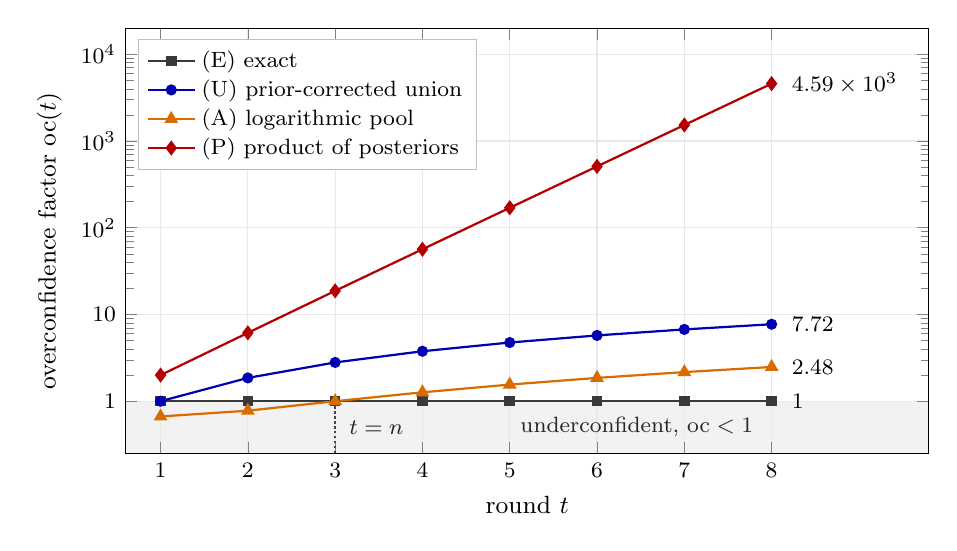
\begin{tikzpicture}
  \begin{semilogyaxis}[name=oc, scale only axis, width=10.2cm, height=5.4cm, set layers,
      xmin=0.6, xmax=9.8, ymin=0.25, ymax=2e4,
      xtick={1,...,8}, ytick={1,10,100,1000,10000}, yticklabels={$1$,$10$,$10^2$,$10^3$,$10^4$},
      xlabel={round $t$}, ylabel={overconfidence factor $\mathrm{oc}(t)$},
      grid=major, grid style={gray!18},
      legend style={font=\footnotesize, at={(0.015,0.975)}, anchor=north west, draw=gray!50, fill=white,
        cells={anchor=west}, row sep=-1pt},
      every axis label/.style={font=\small}, tick label style={font=\footnotesize}]
    \begin{pgfonlayer}{axis background}
      \fill[gray!10] (axis cs:0.6,0.25) rectangle (axis cs:9.8,1);
    \end{pgfonlayer}
    \addplot[gray!45!black, thick, mark=square*, mark size=1.5pt] coordinates {(1,1) (2,1) (3,1) (4,1) (5,1) (6,1) (7,1) (8,1)};
    \addlegendentry{(E) exact}
    \addplot[blue!70!black, thick, mark=*, mark size=1.6pt] coordinates {(1,1) (2,1.8571) (3,2.8) (4,3.7692) (5,4.75) (6,5.7368) (7,6.7273) (8,7.72)};
    \addlegendentry{(U) prior-corrected union}
    \addplot[orange!85!black, thick, mark=triangle*, mark size=2.1pt] coordinates {(1,0.66667) (2,0.77778) (3,1) (4,1.2667) (5,1.5556) (6,1.8571) (7,2.1667) (8,2.4815)};
    \addlegendentry{(A) logarithmic pool}
    \addplot[red!70!black, thick, mark=diamond*, mark size=2.1pt] coordinates {(1,2) (2,6.1429) (3,18.727) (4,56.522) (5,169.92) (6,510.12) (7,1530.7) (8,4592.5)};
    \addlegendentry{(P) product of posteriors}
    % values at t = 8
    \node[font=\footnotesize, anchor=west] at (axis cs:8.12,4592.5) {$4.59\times10^3$};
    \node[font=\footnotesize, anchor=west] at (axis cs:8.12,7.72) {$7.72$};
    \node[font=\footnotesize, anchor=west] at (axis cs:8.12,2.4815) {$2.48$};
    \node[font=\footnotesize, anchor=west] at (axis cs:8.12,1) {$1$};
    % (A) is calibrated at t = n = 3
    \draw[gray!55!black, densely dotted, thick] (axis cs:3,0.25) -- (axis cs:3,1);
    \node[font=\footnotesize, gray!30!black, anchor=west] at (axis cs:3.05,0.5) {$t=n$};
    \node[font=\footnotesize, gray!30!black, anchor=east] at (axis cs:7.9,0.5) {underconfident, $\mathrm{oc}<1$};
  \end{semilogyaxis}
\end{tikzpicture}

  \caption{\textbf{Overconfidence of a record rebuilt from its readers' posteriors.} The overconfidence factor $\mathrm{oc}(t)$ of \cref{tab:hie-records}, the mean-square error of the record's mean times its claimed precision, against the round $t$ on a logarithmic scale for the four aggregation rules of \cref{prop:hie-literal-records}, with three members of unit information and $\Lambda_\circ=1$; the shaded band is $\mathrm{oc}<1$. Exact counting (E) stays at $1$. The prior-corrected union (U) is exact after one round and then grows like $t$, to $7.72$ at $t=8$. The logarithmic pool (A) is underconfident for $t<n$, with $\mathrm{oc}=0.667$ and $0.778$, reaches $\mathrm{oc}=1$ at $t=n=3$ and then grows like $t/n$, to $2.48$. The product of posteriors (P) grows like $n^t$, to $4.59\times10^3$. Over the eight rounds every rule keeps the mean-square error between $1/4$ and $1/3$, so the growth is that of the claimed precision, which at $t=8$ is $25$, $9$ and $16401$ under (U), (A) and (P) against the exact $4$.}
  \label{fig:hie-overconfidence}
\end{figure}

In a changing world a record that is read by memoryless members as their prior and aggregated by rule (U) relative to its prediction equals the centralized Kalman filter, under the hypotheses stated there (Supplement, \cref{prop:hie-record-filter}).

Across levels, literal reading at every level of a scalar tree with unit noiseless links ($\mathsf G=1$, $\Psi=0$) counts a member's own datum once more for each level above the member, and a shortcut to the top that is fused as an independent prior counts the prior and every other datum twice (Supplement, \cref{prop:hie-depth}; see also \cref{rem:hie-literal-consensus,rem:hie-gauge} there).

\subsection{Records as top-down channels}\label{sec:hie-records}

Records that members write and read, such as archives, ledgers and shared notes, are top-down channels. Throughout this subsection a collective $C$ of $n$ members has one global record $z$, read by every member with weight $\beta$ in place of self-weight ($\upsilon=0$) and written by the members' mean with weight $\omega$, with decay $\delta$. In the continuous-time form of \cref{def:fw-record-model} with a uniform kernel on $C$, the global record of \cref{sec:sca-time}, the world-conditional errors obey
\begin{equation}\label{eq:hie-record}
\mathrm de_i=-\Bigl[(\varepsilon+\beta)e_i+\sum_ja_{ij}(e_i-e_j)-\beta z\Bigr]\mathrm dt+\sqrt{2q}\mathrm d\mathsf B_i,\qquad\mathrm dz=-\Bigl[(\omega+\delta)z-\frac\omega n\sum_{i\in C}e_i\Bigr]\mathrm dt+\sqrt{2q_z}\mathrm d\mathsf B_z,
\end{equation}
with symmetric couplings $a_{ij}=a_{ji}\ge0$. We write $L_C$ for the Laplacian of the couplings inside $C$, $\mathcal R=\beta/\omega$, and $\mathsf R=\bigl(\begin{smallmatrix}\varepsilon+\beta&-\beta\\-\omega&\omega+\delta\end{smallmatrix}\bigr)$ for the matrix of the reduced record model of \cref{prop:sca-records}, with eigenvalues $\mathsf r_-\le\mathsf r_+$; the smaller is the effective leak $\varepsilon_{\mathrm{rec}}$.

\begin{proposition}[Drift timescale separation with a global record]\label{prop:hie-record-gain}
Let the exterior of $C$ be held fixed, with uniform cut couplings absorbed into $\varepsilon$.
\begin{enumerate}
\item[(a)] The drift spectrum is $\{\mathsf r_-,\mathsf r_+\}\cup\{\varepsilon+\beta+\lambda_k(L_C):k\ge2\}$, with $\mathsf r_\pm=\frac12\bigl[\varepsilon+\beta+\omega+\delta\pm((\varepsilon+\beta-\omega-\delta)^2+4\beta\omega)^{1/2}\bigr]$; without the record it is $\{\varepsilon\}\cup\{\varepsilon+\lambda_k(L_C):k\ge2\}$.
\item[(b)] The ratio of the second-smallest to the smallest rate changes by the factor
\begin{equation}\label{eq:hie-gain}
\mathsf g_{\mathrm{sep}}=\frac{\varepsilon}{\mathsf r_-}\cdot\frac{\min\{\mathsf r_+,\varepsilon+\beta+\lambda_2(L_C)\}}{\varepsilon+\lambda_2(L_C)}.
\end{equation}
Let $\mathsf g_\times=(1+\mathcal R)(1+\beta/(\varepsilon+\lambda_2(L_C)))$, the product of the record's memory factor and the reading factor.
\item[(c)] For $\delta=0$, $\varepsilon/\mathsf r_-\in[1+\mathcal R,1+\mathcal R+\varepsilon/\omega]$, and if $\lambda_2(L_C)+\varepsilon/(1+\mathcal R)\le\omega$, then $\mathsf g_\times\le\mathsf g_{\mathrm{sep}}\le(1+\mathcal R+\varepsilon/\omega)(1+\beta/(\varepsilon+\lambda_2(L_C)))$.
\item[(d)] If $\mathsf r_+<\varepsilon+\beta+\lambda_2(L_C)$, the second-slowest mode is the exchange between the members' mean and the record, and for every $\delta\ge0$
\begin{equation}\label{eq:hie-gain-ratio}
\frac{\mathsf g_{\mathrm{sep}}}{\mathsf g_\times}=\frac{\varepsilon/\mathsf r_-}{1+\mathcal R}\cdot\frac{\mathsf r_+}{\varepsilon+\beta+\lambda_2(L_C)}<1+\frac{\varepsilon}{\omega(1+\mathcal R)};
\end{equation}
for $\delta=0$ the ratio tends to $(\beta+\omega)/(\beta+\lambda_2(L_C))$ as $\varepsilon\to0$, which is below one when $\omega<\lambda_2(L_C)$.
\item[(e)] For $\delta>0$, $\varepsilon/\mathsf r_-\ge\varepsilon(1+\mathcal R)/(\varepsilon+\mathcal R\delta)$, a bound that exceeds one if and only if $\delta<\varepsilon$.
\end{enumerate}
\end{proposition}
% src: H2-P6; HC_critic V3 (ratio bound (d) replaces the lane's "the gain is smaller")

Proof in \cref{app:hie}; checked in \cref{chk:hie-record-drift}. The record multiplies the memory of the collective mode by about $1+\mathcal R$ and adds $\beta$ to the rate of every internal disagreement, but the product of the two factors is the separation gain only when the record is written faster than the members mix; on a ring of ten members with neighbor coupling $1$, $\varepsilon=0.01$, $\beta=0.2$ and $\omega=0.1$ the gain is $2.40$ against the product $4.53$. For $\delta=0$ a weakly read record lowers the separation of the joint drift spectrum of members and record: when $\mathsf r_+<\varepsilon+\beta+\lambda_2(L_C)$ the identity $\mathsf r_+\mathsf r_-=\varepsilon\omega$ turns \eqref{eq:hie-gain} into $\mathsf g_{\mathrm{sep}}=\mathsf r_+^2/(\omega(\varepsilon+\lambda_2(L_C)))$, and since $\mathsf r_+$ increases with $\beta$, $\mathsf g_{\mathrm{sep}}<1$ exactly for $\beta<(\mathsf r_\circ-\varepsilon)(\mathsf r_\circ-\omega)/\mathsf r_\circ$ with $\mathsf r_\circ=(\omega(\varepsilon+\lambda_2(L_C)))^{1/2}$, a nonempty range exactly when $\max\{\varepsilon,\omega\}<\mathsf r_\circ$, because the second-slowest rate is then the exchange rate $\mathsf r_+$ of the members' mean and the record rather than an internal rate; on the ring of ten this range is $\beta<0.0930$, and $\mathsf g_{\mathrm{sep}}\to\omega/(\varepsilon+\lambda_2(L_C))=0.255$ as $\beta\to0$. In that limit $\mathsf r_+$ tends to the record's own rate $\omega$, here larger than $\varepsilon$, and the members' own rates tend to those without the record, so the lowered separation is a property of the joint spectrum, in which a record that is barely read contributes its own rate, and not a change in the members' dynamics. The memory factor also extends identity under turnover.

\begin{corollary}[Identity gain from a member-written record]\label{cor:hie-identity}
In the setting and under the hypotheses of \cref{prop:agy-identity}, namely turnover rate $g>0$, newcomer noise of positive finite variance and $\det\mathsf A>0$, with newcomer fidelity $\mathsf f$, put $\tilde\varepsilon=\varepsilon+g(1-\mathsf f)$, $\tilde\beta=\beta+g\mathsf f$ and $\tilde{\mathcal R}=\tilde\beta/\omega$. The identity time with the record is that of the pair $(\bar\mu,z)$ of \cref{prop:agy-identity}(a), and for $\tilde\beta>0$ it is also that of the members' mean $\bar\mu$. Divided by the identity time without the record, with newcomers copying the members' mean with the same fidelity, it lies in $[1+\tilde{\mathcal R},1+\tilde{\mathcal R}+\tilde\varepsilon/\omega]$ for $\delta=0$, and is at least $\tilde\varepsilon(1+\tilde{\mathcal R})/(\tilde\varepsilon+\tilde{\mathcal R}\delta)$ for every $\delta\ge0$. For $\tilde\beta=0$ the record is unread, the members' mean has the same identity time with and without it, and a ratio above $1$ concerns the record alone.
\end{corollary}
% src: H2-C1; identification with prop:agy-identity(a) re-derived and checked in the verification round (pvrf_hie)

Proof in \cref{app:hie}; checked in \cref{chk:hie-record-drift}. For a convention, which no member senses, the record is pure gain; for a grounded coordinate it is a top-down prior on the world, paid for in shared error. In the scalar level-0 network of \cref{def:fw-level0} with exact code models, let a collective $C$ closed under attention, with common sensing gain $k^s$, read with gain $\beta$ and read noise $\nu_z$ a record that predicts the world from the members' predicted means, $z(t+1)=F[(1-\omega)z(t)+\omega\bar m_C(t)]$, so that its error $e_z=z-\eta$ joins the members' errors in the error recursion.

\begin{lemma}[Records are blind to shared error and slow its correction]\label{lem:hie-record-blind}
\leavevmode
\begin{enumerate}
\item[(a)] Adding a common process $x(t)$ to every member's error and to the record's error leaves every social innovation $y_{ij}-m_i=e_j-e_i+\nu_{ij}$ and every top-down innovation $z+\nu_z-m_i=e_z-e_i+\nu_z$ unchanged, and shifts every sensory innovation $s_i-m_i=v_i-e_i$ by $-x(t)$: no statistic of social and top-down innovations carries information about a misconception that the members share with their record.
\item[(b)] Let $1-k^s-\beta-\sum_jk_{ij}\ge0$ and $\beta+\omega\le1$, and let $\mathsf N=\bigl(\begin{smallmatrix}1-k^s-\beta&\beta\\\omega&1-\omega\end{smallmatrix}\bigr)$. A common shift $x_0$ at round $0$ evolves, other inputs held fixed, as $x_0(\mathsf f_t\one_C,\mathsf f^z_t)$ with $(\mathsf f_t,\mathsf f^z_t)^\top=(F\mathsf N)^t(1,1)^\top$, coefficients unrelated to the newcomer fidelity $\mathsf f$ of \cref{cor:hie-identity}, and $\mathsf f_t\ge(F(1-k^s))^t$. If $\beta>0$, its asymptotic decay factor per round is $F\mathsf m_1$, with $\mathsf m_1$ the larger eigenvalue of $\mathsf N$ and $1-\mathsf m_1=\varepsilon_{\mathrm{rec}}\in[k^s/(1+\mathcal R+k^s/\omega),k^s/(1+\mathcal R)]$: the record slows the grounding-driven correction of a shared misconception from $k^s$ per round to at most $k^s/(1+\mathcal R)$.
\end{enumerate}
\end{lemma}
% src: H2-L2; extends lem:mis-social-blind

Proof in \cref{app:hie}. Part (a) extends \cref{lem:mis-social-blind} to top-down innovations: a record written by the members agrees with them about every error they share.

\begin{theorem}[The shared-error floor grows with top-down reading]\label{thm:hie-floor}
Let the world be stationary with $0<F<1$ and $Q>0$, the local noises independent of the world innovations, and $\beta,\omega>0$, in the setting of \cref{lem:hie-record-blind}(b). Every member's stationary mean-square error satisfies $\E e_i^2\ge Q\mathsf F_{\mathrm{com}}$, where $\mathsf F_{\mathrm{com}}=\sum_{s\ge0}\mathsf f_s^2$ is the variance factor of the common mode, and:
\begin{enumerate}
\item[(a)] with $\mathsf m_1>\mathsf m_2$ the eigenvalues of $\mathsf N$, $\mathsf c_1=(1-k^s-\mathsf m_2)/(\mathsf m_1-\mathsf m_2)>0$ and $\mathsf c_2=(\mathsf m_1-1+k^s)/(\mathsf m_1-\mathsf m_2)\ge0$,
\begin{equation}\label{eq:hie-floor}
\mathsf F_{\mathrm{com}}=\frac{\mathsf c_1^2}{1-F^2\mathsf m_1^2}+\frac{2\mathsf c_1\mathsf c_2}{1-F^2\mathsf m_1\mathsf m_2}+\frac{\mathsf c_2^2}{1-F^2\mathsf m_2^2};
\end{equation}
\item[(b)] $\mathsf F_{\mathrm{com}}\ge1/(1-F^2(1-k^s)^2)$, the factor of the floor of \cref{prop:mis-mse-floor} without the record, strictly when $k^s>0$;
\item[(c)] $\mathsf F_{\mathrm{com}}$ is nondecreasing in $\beta$ and nonincreasing in $\omega$;
\item[(d)] $\mathsf F_{\mathrm{com}}\ge\mathsf c_1^2/(1-F^2(1-k^s/(1+\mathcal R))^2)$, and $\mathsf c_1\to1$ as $k^s\to0$;
\item[(e)] $\mathsf F_{\mathrm{com}}<(1+\mathcal R)/(1-F^2(1-k^s)^2)$, and at fixed $\beta$ and $\omega$, if $k^s\to0$ and $F\to1$ with $(1-F)/k^s\to\mathsf y\in[0,\infty)$, then $\mathsf F_{\mathrm{com}}(1-F^2(1-k^s)^2)\to(1+\mathsf y)(1+\mathcal R)/(1+\mathsf y(1+\mathcal R))$, which is $1+\mathcal R$ at $\mathsf y=0$.
\end{enumerate}
\end{theorem}
% src: H2-T2; HC_critic V3; (e) proved in the verification round (pvrf_hie_sym, pvrf_hie), replacing the numerical support of "up to 1+R"

\begin{figure}[!t]
  \centering
  % Figure: records buy memory with shared error (prop:hie-record-gain, thm:hie-floor).
% (a) Ring of n = 10 members with neighbor coupling 1, so lambda_k(L_C) = 2 - 2cos(2 pi k/10): 0.38197, 1.38197,
%     2.61803 and 3.61803 twice each and 4 once for k >= 2; eps = 0.01, omega = 0.1, delta = 0, one global record
%     read with weight beta in place of self-weight; 51 values of beta in [0, 1].
%     Upper plot: drift spectrum of eq:hie-record by prop:hie-record-gain(a), the rates
%       r_pm = (1/2)[eps + beta + omega + delta +- ((eps + beta - omega - delta)^2 + 4 beta omega)^(1/2)]
%     of the members' mean and the record, and the internal rates eps + beta + lambda_k(L_C), k >= 2. The
%     eigenvalues of the full 11 x 11 drift agree with these to a relative deviation 8.4e-13.
%     Lower plot: the separation gain g_sep of eq:hie-gain and the product g_x = (1 + R)(1 + beta/(eps + lambda_2(L_C))),
%     R = beta/omega; g_sep from the full spectrum agrees with eq:hie-gain to 8.4e-13. Since omega < lambda_2(L_C),
%     r_+ < eps + beta + omega < eps + beta + lambda_2(L_C) for every beta, so the second-slowest mode is the exchange
%     of mean and record, and g_sep/g_x stays within 3.1 percent of its eps -> 0 limit (beta + omega)/(beta + lambda_2)
%     of prop:hie-record-gain(d), at most 0.803. At beta = 0.2: r_- = 0.003260 against eps/(1 + R) = 0.003333,
%     r_+ = 0.3067, g_sep = 2.400 against g_x = 4.531, the values of chk:hie-record-drift. g_sep -> omega/(eps +
%     lambda_2) = 0.255 as beta -> 0, g_sep = 1 at beta = 0.0930, and g_sep = 31.38 against g_x = 39.06 at beta = 1.
% (b) Common-mode factor F_com of eq:hie-floor, F_com = c_1^2/(1 - F^2 m_1^2) + 2 c_1 c_2/(1 - F^2 m_1 m_2)
%     + c_2^2/(1 - F^2 m_2^2) with m_1 > m_2 the eigenvalues of N = [[1 - k^s - beta, beta], [omega, 1 - omega]],
%     divided by its value 1/(1 - F^2 (1 - k^s)^2) without the record (thm:hie-floor(b)), against 1 + R with
%     beta = R omega; 46 points per curve, logarithmic axes. F = 0.9, 0.99, 0.999 at k^s = 0.05, omega = 0.1
%     (beta from 0 to 0.9); F = 0.9999 at k^s = 0.02, omega = 0.05 (beta from 0 to 0.45). The closed form agrees
%     with the series sum_s f_s^2 and with a Stein-equation solve to 2.2e-13. Marked: 1.113, 1.936, 2.553 for
%     F = 0.9, 0.99, 0.999 at beta = 0.2 (1 + R = 3), and 8.240 for F = 0.9999 at beta = 0.4 (1 + R = 9), where
%     F_com = 207.1 against 25.13, the values of chk:hie-record-drift. At 1 + R = 10 the ratios are 1.267, 3.620,
%     7.892 and 9.141. No curve exceeds the dashed line 1 + R. Data are embedded as computed, in double precision.
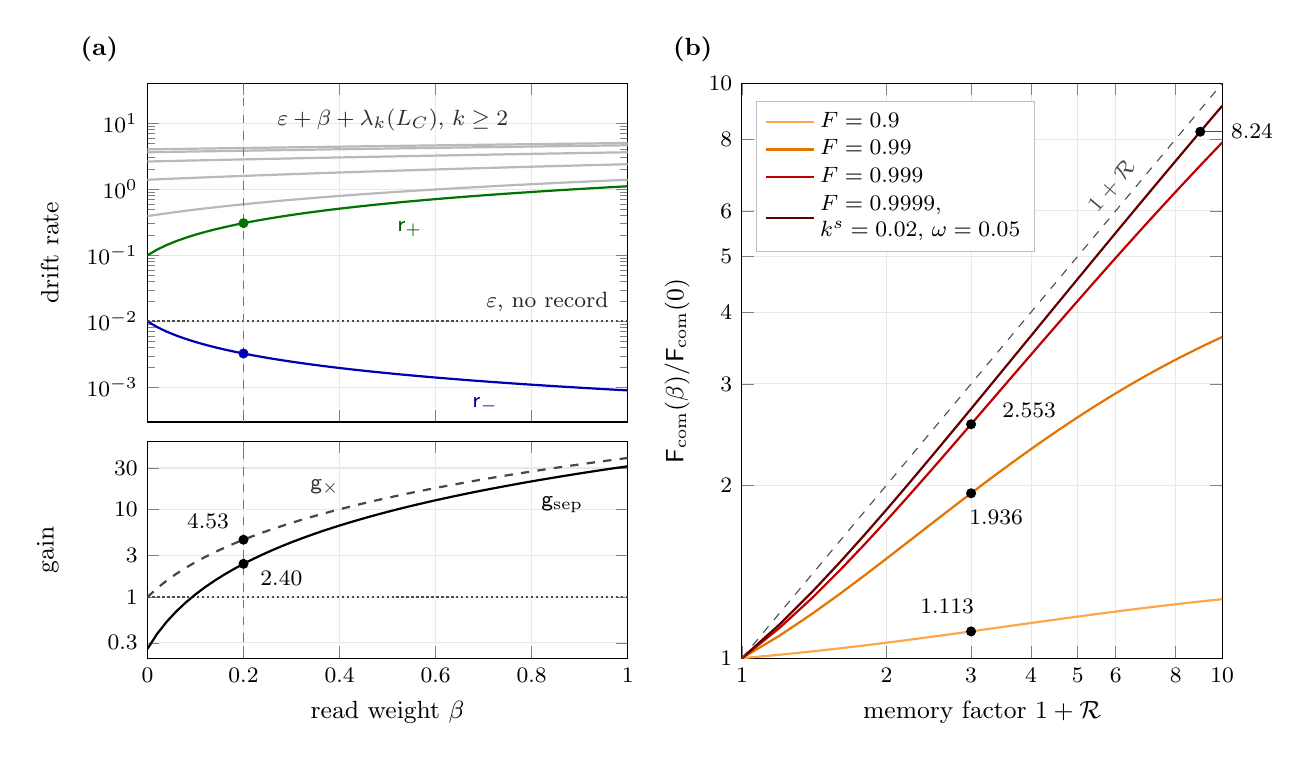
\begin{tikzpicture}
  \pgfplotsset{recframe/.style={scale only axis, width=6.1cm, grid=major, grid style={gray!18},
      every axis label/.style={font=\small}, tick label style={font=\footnotesize}},
    leftlabel/.style={every axis y label/.style={font=\small, rotate=90, at={(axis description cs:-0.165,0.5)}, anchor=south}}}
  % panel (a), upper plot: drift spectrum
  \begin{semilogyaxis}[recframe, leftlabel, name=spec, height=4.3cm, xmin=0, xmax=1, ymin=3e-4, ymax=40,
      xticklabels={}, ytick={1e-3,1e-2,1e-1,1,10}, ylabel={drift rate}]
    \addplot[gray!55, thick] coordinates {(0,0.39197) (0.02,0.41197) (0.04,0.43197) (0.06,0.45197) (0.08,0.47197) (0.1,0.49197) (0.12,0.51197) (0.14,0.53197) (0.16,0.55197) (0.18,0.57197) (0.2,0.59197) (0.22,0.61197) (0.24,0.63197) (0.26,0.65197) (0.28,0.67197) (0.3,0.69197) (0.32,0.71197) (0.34,0.73197) (0.36,0.75197) (0.38,0.77197) (0.4,0.79197) (0.42,0.81197) (0.44,0.83197) (0.46,0.85197) (0.48,0.87197) (0.5,0.89197) (0.52,0.91197) (0.54,0.93197) (0.56,0.95197) (0.58,0.97197) (0.6,0.99197) (0.62,1.012) (0.64,1.032) (0.66,1.052) (0.68,1.072) (0.7,1.092) (0.72,1.112) (0.74,1.132) (0.76,1.152) (0.78,1.172) (0.8,1.192) (0.82,1.212) (0.84,1.232) (0.86,1.252) (0.88,1.272) (0.9,1.292) (0.92,1.312) (0.94,1.332) (0.96,1.352) (0.98,1.372) (1,1.392)};
    \addplot[gray!55, thick] coordinates {(0,1.392) (0.02,1.412) (0.04,1.432) (0.06,1.452) (0.08,1.472) (0.1,1.492) (0.12,1.512) (0.14,1.532) (0.16,1.552) (0.18,1.572) (0.2,1.592) (0.22,1.612) (0.24,1.632) (0.26,1.652) (0.28,1.672) (0.3,1.692) (0.32,1.712) (0.34,1.732) (0.36,1.752) (0.38,1.772) (0.4,1.792) (0.42,1.812) (0.44,1.832) (0.46,1.852) (0.48,1.872) (0.5,1.892) (0.52,1.912) (0.54,1.932) (0.56,1.952) (0.58,1.972) (0.6,1.992) (0.62,2.012) (0.64,2.032) (0.66,2.052) (0.68,2.072) (0.7,2.092) (0.72,2.112) (0.74,2.132) (0.76,2.152) (0.78,2.172) (0.8,2.192) (0.82,2.212) (0.84,2.232) (0.86,2.252) (0.88,2.272) (0.9,2.292) (0.92,2.312) (0.94,2.332) (0.96,2.352) (0.98,2.372) (1,2.392)};
    \addplot[gray!55, thick] coordinates {(0,2.628) (0.02,2.648) (0.04,2.668) (0.06,2.688) (0.08,2.708) (0.1,2.728) (0.12,2.748) (0.14,2.768) (0.16,2.788) (0.18,2.808) (0.2,2.828) (0.22,2.848) (0.24,2.868) (0.26,2.888) (0.28,2.908) (0.3,2.928) (0.32,2.948) (0.34,2.968) (0.36,2.988) (0.38,3.008) (0.4,3.028) (0.42,3.048) (0.44,3.068) (0.46,3.088) (0.48,3.108) (0.5,3.128) (0.52,3.148) (0.54,3.168) (0.56,3.188) (0.58,3.208) (0.6,3.228) (0.62,3.248) (0.64,3.268) (0.66,3.288) (0.68,3.308) (0.7,3.328) (0.72,3.348) (0.74,3.368) (0.76,3.388) (0.78,3.408) (0.8,3.428) (0.82,3.448) (0.84,3.468) (0.86,3.488) (0.88,3.508) (0.9,3.528) (0.92,3.548) (0.94,3.568) (0.96,3.588) (0.98,3.608) (1,3.628)};
    \addplot[gray!55, thick] coordinates {(0,3.628) (0.02,3.648) (0.04,3.668) (0.06,3.688) (0.08,3.708) (0.1,3.728) (0.12,3.748) (0.14,3.768) (0.16,3.788) (0.18,3.808) (0.2,3.828) (0.22,3.848) (0.24,3.868) (0.26,3.888) (0.28,3.908) (0.3,3.928) (0.32,3.948) (0.34,3.968) (0.36,3.988) (0.38,4.008) (0.4,4.028) (0.42,4.048) (0.44,4.068) (0.46,4.088) (0.48,4.108) (0.5,4.128) (0.52,4.148) (0.54,4.168) (0.56,4.188) (0.58,4.208) (0.6,4.228) (0.62,4.248) (0.64,4.268) (0.66,4.288) (0.68,4.308) (0.7,4.328) (0.72,4.348) (0.74,4.368) (0.76,4.388) (0.78,4.408) (0.8,4.428) (0.82,4.448) (0.84,4.468) (0.86,4.488) (0.88,4.508) (0.9,4.528) (0.92,4.548) (0.94,4.568) (0.96,4.588) (0.98,4.608) (1,4.628)};
    \addplot[gray!55, thick] coordinates {(0,4.01) (0.02,4.03) (0.04,4.05) (0.06,4.07) (0.08,4.09) (0.1,4.11) (0.12,4.13) (0.14,4.15) (0.16,4.17) (0.18,4.19) (0.2,4.21) (0.22,4.23) (0.24,4.25) (0.26,4.27) (0.28,4.29) (0.3,4.31) (0.32,4.33) (0.34,4.35) (0.36,4.37) (0.38,4.39) (0.4,4.41) (0.42,4.43) (0.44,4.45) (0.46,4.47) (0.48,4.49) (0.5,4.51) (0.52,4.53) (0.54,4.55) (0.56,4.57) (0.58,4.59) (0.6,4.61) (0.62,4.63) (0.64,4.65) (0.66,4.67) (0.68,4.69) (0.7,4.71) (0.72,4.73) (0.74,4.75) (0.76,4.77) (0.78,4.79) (0.8,4.81) (0.82,4.83) (0.84,4.85) (0.86,4.87) (0.88,4.89) (0.9,4.91) (0.92,4.93) (0.94,4.95) (0.96,4.97) (0.98,4.99) (1,5.01)};
    \addplot[green!45!black, thick] coordinates {(0,0.1) (0.02,0.12179) (0.04,0.14301) (0.06,0.1639) (0.08,0.18458) (0.1,0.20512) (0.12,0.22557) (0.14,0.24593) (0.16,0.26624) (0.18,0.28651) (0.2,0.30674) (0.22,0.32694) (0.24,0.34712) (0.26,0.36728) (0.28,0.38742) (0.3,0.40755) (0.32,0.42766) (0.34,0.44777) (0.36,0.46786) (0.38,0.48795) (0.4,0.50803) (0.42,0.52811) (0.44,0.54818) (0.46,0.56824) (0.48,0.5883) (0.5,0.60836) (0.52,0.62841) (0.54,0.64846) (0.56,0.6685) (0.58,0.68855) (0.6,0.70859) (0.62,0.72863) (0.64,0.74866) (0.66,0.7687) (0.68,0.78873) (0.7,0.80876) (0.72,0.82879) (0.74,0.84882) (0.76,0.86885) (0.78,0.88887) (0.8,0.9089) (0.82,0.92892) (0.84,0.94895) (0.86,0.96897) (0.88,0.98899) (0.9,1.009) (0.92,1.029) (0.94,1.049) (0.96,1.0691) (0.98,1.0891) (1,1.1091)};
    \addplot[blue!70!black, thick] coordinates {(0,0.01) (0.02,0.0082109) (0.04,0.0069926) (0.06,0.0061013) (0.08,0.0054176) (0.1,0.0048751) (0.12,0.0044333) (0.14,0.0040661) (0.16,0.003756) (0.18,0.0034903) (0.2,0.0032601) (0.22,0.0030587) (0.24,0.0028809) (0.26,0.0027227) (0.28,0.0025812) (0.3,0.0024537) (0.32,0.0023383) (0.34,0.0022333) (0.36,0.0021374) (0.38,0.0020494) (0.4,0.0019684) (0.42,0.0018936) (0.44,0.0018242) (0.46,0.0017598) (0.48,0.0016998) (0.5,0.0016438) (0.52,0.0015913) (0.54,0.0015421) (0.56,0.0014959) (0.58,0.0014523) (0.6,0.0014113) (0.62,0.0013724) (0.64,0.0013357) (0.66,0.0013009) (0.68,0.0012679) (0.7,0.0012365) (0.72,0.0012066) (0.74,0.0011781) (0.76,0.0011509) (0.78,0.001125) (0.8,0.0011002) (0.82,0.0010765) (0.84,0.0010538) (0.86,0.001032) (0.88,0.0010111) (0.9,0.00099107) (0.92,0.00097179) (0.94,0.00095325) (0.96,0.0009354) (0.98,0.0009182) (1,0.00090163)};
    \draw[gray!60!black, densely dotted, thick] (axis cs:0,0.01) -- (axis cs:1,0.01);
    \draw[black!55, dashed] (axis cs:0.2,3e-4) -- (axis cs:0.2,40);
    \addplot[only marks, mark=*, mark size=1.6pt, blue!70!black] coordinates {(0.2,0.0032601)};
    \addplot[only marks, mark=*, mark size=1.6pt, green!45!black] coordinates {(0.2,0.30674)};
    \node[font=\footnotesize, gray!35!black, anchor=south west] at (axis cs:0.25,5.5) {$\varepsilon+\beta+\lambda_k(L_C)$, $k\ge2$};
    \node[font=\footnotesize, green!35!black, anchor=north west] at (axis cs:0.5,0.46) {$\mathsf r_+$};
    \node[font=\footnotesize, blue!60!black, anchor=north east] at (axis cs:0.75,1.0e-3) {$\mathsf r_-$};
    \node[font=\footnotesize, gray!30!black, anchor=south east] at (axis cs:0.98,0.01) {$\varepsilon$, no record};
  \end{semilogyaxis}
  \node[font=\small\bfseries, anchor=south east] at ($(spec.north west)+(-0.25cm,0.15cm)$) {(a)};
  % panel (a), lower plot: separation gain
  \begin{semilogyaxis}[recframe, leftlabel, name=gain, height=2.75cm, at={($(spec.south west)+(0,-0.25cm)$)}, anchor=north west,
      xmin=0, xmax=1, ymin=0.2, ymax=60, ytick={0.3,1,3,10,30}, log ticks with fixed point,
      xlabel={read weight $\beta$}, ylabel={gain}]
    \draw[gray!60!black, densely dotted, thick] (axis cs:0,1) -- (axis cs:1,1);
    \draw[black!55, dashed] (axis cs:0.2,0.2) -- (axis cs:0.2,60);
    \addplot[gray!55!black, thick, dashed] coordinates {(0,1) (0.02,1.2612) (0.04,1.5429) (0.06,1.8449) (0.08,2.1674) (0.1,2.5102) (0.12,2.8735) (0.14,3.2572) (0.16,3.6613) (0.18,4.0858) (0.2,4.5307) (0.22,4.9961) (0.24,5.4818) (0.26,5.988) (0.28,6.5145) (0.3,7.0615) (0.32,7.6289) (0.34,8.2167) (0.36,8.8249) (0.38,9.4535) (0.4,10.102) (0.42,10.772) (0.44,11.462) (0.46,12.172) (0.48,12.903) (0.5,13.654) (0.52,14.425) (0.54,15.217) (0.56,16.029) (0.58,16.862) (0.6,17.715) (0.62,18.589) (0.64,19.483) (0.66,20.397) (0.68,21.332) (0.7,22.287) (0.72,23.263) (0.74,24.259) (0.76,25.275) (0.78,26.312) (0.8,27.369) (0.82,28.447) (0.84,29.545) (0.86,30.663) (0.88,31.802) (0.9,32.961) (0.92,34.141) (0.94,35.341) (0.96,36.561) (0.98,37.802) (1,39.064)};
    \addplot[black, thick] coordinates {(0,0.25512) (0.02,0.37841) (0.04,0.52176) (0.06,0.68533) (0.08,0.86922) (0.1,1.0735) (0.12,1.2981) (0.14,1.5431) (0.16,1.8085) (0.18,2.0943) (0.2,2.4004) (0.22,2.727) (0.24,3.074) (0.26,3.4414) (0.28,3.8292) (0.3,4.2375) (0.32,4.6661) (0.34,5.1151) (0.36,5.5846) (0.38,6.0744) (0.4,6.5847) (0.42,7.1153) (0.44,7.6664) (0.46,8.2379) (0.48,8.8298) (0.5,9.4421) (0.52,10.075) (0.54,10.728) (0.56,11.401) (0.58,12.095) (0.6,12.81) (0.62,13.544) (0.64,14.3) (0.66,15.075) (0.68,15.871) (0.7,16.688) (0.72,17.524) (0.74,18.382) (0.76,19.259) (0.78,20.157) (0.8,21.076) (0.82,22.015) (0.84,22.974) (0.86,23.954) (0.88,24.954) (0.9,25.974) (0.92,27.015) (0.94,28.076) (0.96,29.158) (0.98,30.26) (1,31.383)};
    \addplot[only marks, mark=*, mark size=1.6pt, black] coordinates {(0.2,2.4004) (0.2,4.5307)};
    \node[font=\footnotesize, anchor=south east] at (axis cs:0.19,4.75) {$4.53$};
    \node[font=\footnotesize, anchor=west] at (axis cs:0.215,1.65) {$2.40$};
    \node[font=\footnotesize, gray!40!black, anchor=south east] at (axis cs:0.42,11.5) {$\mathsf g_\times$};
    \node[font=\footnotesize, anchor=north west] at (axis cs:0.8,18) {$\mathsf g_{\mathrm{sep}}$};
  \end{semilogyaxis}
  % panel (b): common-mode factor with the record over its value without
  \begin{loglogaxis}[recframe, name=floor, at={($(spec.north east)+(1.45cm,0)$)}, anchor=north west, height=7.3cm,
      clip=false, xmin=1, xmax=10, ymin=1, ymax=10, xtick={1,2,3,4,5,6,8,10}, ytick={1,2,3,4,5,6,8,10},
      log ticks with fixed point,
      xlabel={memory factor $1+\mathcal R$}, ylabel={$\mathsf F_{\mathrm{com}}(\beta)/\mathsf F_{\mathrm{com}}(0)$},
      legend style={font=\footnotesize, at={(0.03,0.97)}, anchor=north west, draw=gray!50, fill=white,
        cells={anchor=west, align=left}, row sep=-1pt}]
    \addplot[orange!70, thick] coordinates {(1,1) (1.2,1.014) (1.4,1.0275) (1.6,1.0403) (1.8,1.0525) (2,1.0641) (2.2,1.075) (2.4,1.0854) (2.6,1.0952) (2.8,1.1046) (3,1.1134) (3.2,1.1218) (3.4,1.1298) (3.6,1.1374) (3.8,1.1446) (4,1.1514) (4.2,1.158) (4.4,1.1642) (4.6,1.1702) (4.8,1.1759) (5,1.1813) (5.2,1.1865) (5.4,1.1915) (5.6,1.1963) (5.8,1.2009) (6,1.2053) (6.2,1.2095) (6.4,1.2135) (6.6,1.2175) (6.8,1.2212) (7,1.2249) (7.2,1.2284) (7.4,1.2317) (7.6,1.235) (7.8,1.2381) (8,1.2412) (8.2,1.2441) (8.4,1.2469) (8.6,1.2497) (8.8,1.2524) (9,1.2549) (9.2,1.2574) (9.4,1.2599) (9.6,1.2622) (9.8,1.2645) (10,1.2667)};
    \addlegendentry{$F=0.9$}
    \addplot[orange!90!black, thick] coordinates {(1,1) (1.2,1.0956) (1.4,1.1945) (1.6,1.2942) (1.8,1.3931) (2,1.4902) (2.2,1.585) (2.4,1.6772) (2.6,1.7665) (2.8,1.8528) (3,1.9362) (3.2,2.0168) (3.4,2.0944) (3.6,2.1693) (3.8,2.2416) (4,2.3113) (4.2,2.3785) (4.4,2.4433) (4.6,2.5059) (4.8,2.5664) (5,2.6247) (5.2,2.6811) (5.4,2.7356) (5.6,2.7883) (5.8,2.8393) (6,2.8887) (6.2,2.9365) (6.4,2.9828) (6.6,3.0276) (6.8,3.0711) (7,3.1133) (7.2,3.1542) (7.4,3.1939) (7.6,3.2324) (7.8,3.2699) (8,3.3063) (8.2,3.3417) (8.4,3.3761) (8.6,3.4096) (8.8,3.4421) (9,3.4739) (9.2,3.5047) (9.4,3.5348) (9.6,3.5641) (9.8,3.5927) (10,3.6205)};
    \addlegendentry{$F=0.99$}
    \addplot[red!75!black, thick] coordinates {(1,1) (1.2,1.1308) (1.4,1.2728) (1.6,1.4225) (1.8,1.5774) (2,1.7359) (2.2,1.8969) (2.4,2.0596) (2.6,2.2234) (2.8,2.3879) (3,2.5528) (3.2,2.7177) (3.4,2.8825) (3.6,3.0471) (3.8,3.2112) (4,3.3748) (4.2,3.5378) (4.4,3.7002) (4.6,3.8618) (4.8,4.0226) (5,4.1827) (5.2,4.3419) (5.4,4.5003) (5.6,4.6578) (5.8,4.8145) (6,4.9702) (6.2,5.125) (6.4,5.2789) (6.6,5.4319) (6.8,5.5839) (7,5.7351) (7.2,5.8853) (7.4,6.0345) (7.6,6.1829) (7.8,6.3303) (8,6.4768) (8.2,6.6224) (8.4,6.7671) (8.6,6.9109) (8.8,7.0537) (9,7.1957) (9.2,7.3368) (9.4,7.477) (9.6,7.6163) (9.8,7.7547) (10,7.8922)};
    \addlegendentry{$F=0.999$}
    \addplot[red!40!black, thick] coordinates {(1,1) (1.2,1.1466) (1.4,1.304) (1.6,1.4689) (1.8,1.6391) (2,1.8132) (2.2,1.9902) (2.4,2.1694) (2.6,2.3502) (2.8,2.5323) (3,2.7154) (3.2,2.8993) (3.4,3.0838) (3.6,3.2687) (3.8,3.4539) (4,3.6393) (4.2,3.8249) (4.4,4.0106) (4.6,4.1963) (4.8,4.382) (5,4.5677) (5.2,4.7532) (5.4,4.9387) (5.6,5.124) (5.8,5.3091) (6,5.4941) (6.2,5.6789) (6.4,5.8634) (6.6,6.0478) (6.8,6.2319) (7,6.4158) (7.2,6.5994) (7.4,6.7828) (7.6,6.9659) (7.8,7.1487) (8,7.3313) (8.2,7.5136) (8.4,7.6956) (8.6,7.8773) (8.8,8.0587) (9,8.2398) (9.2,8.4207) (9.4,8.6012) (9.6,8.7815) (9.8,8.9614) (10,9.1411)};
    \addlegendentry{$F=0.9999$,\\$k^s=0.02$, $\omega=0.05$}
    \draw[gray!60!black, dashed] (axis cs:1,1) -- (axis cs:10,10) node[pos=0.8, sloped, above, font=\footnotesize] {$1+\mathcal R$};
    \addplot[only marks, mark=*, mark size=1.6pt, black] coordinates {(3,1.1134) (3,1.9362) (3,2.5528) (9,8.2398)};
    \node[font=\footnotesize, inner sep=1pt, anchor=west] at (axis cs:2.316,1.2285) {$1.113$};
    \node[font=\footnotesize, inner sep=1pt, anchor=west] at (axis cs:2.9271,1.757) {$1.936$};
    \node[font=\footnotesize, inner sep=1pt, anchor=west] at (axis cs:3.4300,2.6950) {$2.553$};
    \draw[gray!60!black] (axis cs:9.15,8.2398) -- (axis cs:10,8.2398) node[font=\footnotesize, text=black, inner sep=1pt, anchor=west, xshift=2pt] {$8.24$};
  \end{loglogaxis}
  \node[font=\small\bfseries, anchor=south east] at ($(floor.north west)+(-0.25cm,0.15cm)$) {(b)};
\end{tikzpicture}

  \caption{\textbf{Records buy memory with shared error.} (a) A ring of ten members with neighbor coupling $1$, $\varepsilon=0.01$, $\omega=0.1$ and $\delta=0$, and a global record read with weight $\beta$ in place of self-weight. Upper plot: the drift spectrum of \cref{prop:hie-record-gain}(a), the rates $\mathsf r_-$ of the slow collective mode and $\mathsf r_+$ of the exchange between the members' mean and the record, and the internal rates $\varepsilon+\beta+\lambda_k(L_C)$, $k\ge2$; without the record the slowest rate is $\varepsilon$ (dotted). Lower plot: the separation gain $\mathsf g_{\mathrm{sep}}$ of \eqref{eq:hie-gain} and the product $\mathsf g_\times$ of the memory factor and the reading factor (dashed). Here $\omega<\lambda_2(L_C)=0.382$: the record is written more slowly than the members mix, $\mathsf r_+$ is the second-slowest rate at every $\beta$, and the gain stays below the product, with a ratio within $3.1$ percent of its limit $(\beta+\omega)/(\beta+\lambda_2(L_C))$ as $\varepsilon\to0$ in \cref{prop:hie-record-gain}(d). For $\beta<0.093$ the gain is below one, because the second-slowest rate of the joint spectrum of members and record falls from $\varepsilon+\lambda_2(L_C)$ to $\mathsf r_+=\varepsilon+\beta+\omega-\mathsf r_-$, which tends to the record's own rate $\omega$ as $\beta\to0$, by a larger factor than the slowest rate falls from $\varepsilon$ to $\mathsf r_-$. At $\beta=0.2$ (vertical dashed line), $\mathsf r_-=0.003260$ against $\varepsilon/(1+\mathcal R)=0.003333$ and $\mathsf r_+=0.3067$, and the gain is $2.40$ against the product $4.53$. (b) The common-mode factor $\mathsf F_{\mathrm{com}}(\beta)$ of \eqref{eq:hie-floor} divided by its value $\mathsf F_{\mathrm{com}}(0)=1/(1-F^2(1-k^s)^2)$ without the record, against the memory factor $1+\mathcal R$ on logarithmic axes, for $F=0.9$, $0.99$ and $0.999$ with $k^s=0.05$ and $\omega=0.1$, and for $F=0.9999$ with $k^s=0.02$ and $\omega=0.05$. The marked values are $1.113$, $1.936$ and $2.553$ at $\beta=0.2$, where $1+\mathcal R=3$, and $8.24$ at $\beta=0.4$, where $1+\mathcal R=9$ and $\mathsf F_{\mathrm{com}}$ is $207.1$ against $25.13$. By \cref{thm:hie-floor}(e) the ratio stays below $1+\mathcal R$ (dashed) and approaches it in a persistent world with weak grounding, $k^s\to0$ with $1-F\ll k^s/(1+\mathcal R)$: the memory that the record buys in (a) is paid for in shared error.}
  \label{fig:hie-records}
\end{figure}

Proof in \cref{app:hie}; checked in \cref{chk:hie-record-drift}. By (b) and (e) the record multiplies the shared-error floor by a factor between $1$ and $1+\mathcal R$, the factor by which it lengthens memory and identity, and by (e) the factor approaches $1+\mathcal R$ in a persistent world with weak grounding, $k^s\to0$ with $1-F\ll k^s/(1+\mathcal R)$; at $F=0.9999$, $k^s=0.02$, $\beta=0.4$ and $\omega=0.05$, where $1+\mathcal R=9$, the floor grows by $8.24$. \Cref{fig:hie-records} shows both sides of the exchange: the drift spectrum and separation gain of the ring of ten under a global record, and the shared-error floor rising toward $1+\mathcal R$ as the world becomes persistent. This is the grounding tension of \cref{thm:coh-grounding-tension} across levels, and by \cref{lem:hie-record-blind} the members cannot see its price in their innovations. Records can also read records.

For a chain of nested records with read-to-write ratios $\mathcal R_k$ and leaks only at the agents, $\varepsilon_{\mathrm{rec}}\le\varepsilon/(1+\mathcal R_1+\mathcal R_1\mathcal R_2+\cdots)$, a case of a bound for records arranged on a tree (Supplement, \cref{prop:hie-nested-records}).

Drift is not precision. At the reversible record noise the precision of the population with the record as a node is diffusive, and for $\delta=0$, under the condition on $\beta$ stated there, the contrast of the collective with its record exceeds that of the collective alone by a factor that does not depend on $\omega$, so the memory factor $1+\mathcal R$ is absent from contrast (Supplement, \cref{prop:hie-record-contrast,rem:hie-memory-absent}).

Away from the reversible noise the precision with the record node can leave the diffusive class (Supplement, \cref{ex:hie-noiseless-record}, and the numerical observation \cref{obs:hie-record-window}); at that noise, for a closed population with $\delta=0$, a global record adds to the members' covariance a component common to all pairs (\cref{prop:hie-global-record}).

The weight that a top-down prior deserves is treated in the Supplement (\cref{sec:hie-balance}): under the cavity condition, weight above the Kalman value trades disagreement for shared error (\cref{prop:hie-echo-tradeoff}), and positive precision on a member-written record of a grounded coordinate strictly raises the common-mode part of every member's stationary error under the hypotheses stated there (\cref{conj:hie-top-down}), while the total error was computed only in instances (\cref{obs:hie-top-down}, a numerical observation).

\subsection{Conformity to a self-constituted prior}\label{sec:hie-conformity}

A collective prior can also act on conventions, which no member senses, and conformity is then a candidate mechanism of formation that does not rest on misreading evidence. Let agents hold conventions $\mathsf x_i\in\R$ and expected free energies
\begin{equation}\label{eq:hie-conformity}
G_i(\mathsf x)=\sum_jJ_{ij}(\mathsf x-\mathsf x_j)^2+\mathsf a_{\mathrm p}(\mathsf x-\mathsf x^0_i)^2+\beta_{\mathrm r}(\mathsf x-\bar z_{\alpha,-i})^2,
\end{equation}
up to terms free of $\mathsf x$, with exogenous symmetric attended couplings $J_{ij}=J_{ji}\ge0$, a pragmatic preference for matching attended partners; a pull $\mathsf a_{\mathrm p}>0$ toward a native convention $\mathsf x^0_i$; readership groups $\mathcal K_1,\dots,\mathcal K_{n_{\mathrm g}}$ of sizes $n_\alpha\ge2$ partitioning the agents; and the cavity reading $\bar z_{\alpha,-i}$ of the record of $i$'s group $\mathcal K_\alpha$, the mean of the other members' conventions. Write $L_J$ for the Laplacian of $J$ and $L^{\mathrm{cpl}}_\alpha$ for that of the complete graph with unit weights on $\mathcal K_\alpha$.

\begin{proposition}[Linear conformity cannot form collectives]\label{prop:hie-conformity}
\begin{enumerate}
\item[(a)] $\mathcal V(\mathsf x)=\sum_{i<j}J_{ij}(\mathsf x_i-\mathsf x_j)^2+\mathsf a_{\mathrm p}\sum_i(\mathsf x_i-\mathsf x^0_i)^2+\sum_\alpha\frac{\beta_{\mathrm r}}{n_\alpha-1}\sum_{i<j\in\mathcal K_\alpha}(\mathsf x_i-\mathsf x_j)^2$ is an exact potential. A literal reading in which the record's mean includes the agent's own convention also gives a potential game, with group coupling $\beta_{\mathrm r}(n_\alpha-1)/n_\alpha^2$ in place of $\beta_{\mathrm r}/(n_\alpha-1)$.
\item[(b)] Asynchronous revision at policy precision $\gamma$, in which a uniformly chosen agent samples $\mathsf x_i$ from $q_i\propto e^{-\gamma G_i}$, is the random-scan Gibbs sampler of $e^{-\gamma\mathcal V}$, and its unique stationary law is Gaussian with precision $\Pi=2\gamma(L_J+\mathsf a_{\mathrm p}I+\sum_\alpha\frac{\beta_{\mathrm r}}{n_\alpha-1}L^{\mathrm{cpl}}_\alpha)$, diffusive with leaks $2\gamma\mathsf a_{\mathrm p}$. There is no world to condition on, and contrast is computed from this Gibbs precision.
\item[(c)] A readership group has contrast $r(\mathcal K_\alpha)=(\mathsf a_{\mathrm p}+\lambda_2(L_{J,\alpha})+\beta_{\mathrm r}n_\alpha/(n_\alpha-1))/(\mathsf a_{\mathrm p}+\cut_J(\mathcal K_\alpha)/n_\alpha)$, with $L_{J,\alpha}$ the Laplacian of $J$ inside $\mathcal K_\alpha$: the record adds $\beta_{\mathrm r}n_\alpha/(n_\alpha-1)$ to the internal rate.
\item[(d)] The stationary law, and with it the contrast of every region, is a fixed function of $J$, $\mathsf a_{\mathrm p}$, $\beta_{\mathrm r}$ and the readership groups that does not depend on the initial state, so linear conformity selects no partition that these do not already contain. Which regions are collectives depends on the declared geometry of \cref{def:col-baseline}: no region exceeds the baseline when the comparison medium is the population itself, as under the graph clause when $\Pi$ has equal couplings on the declared edges and uniform leak; the whole population is never a collective when a group of permutations preserving the declared geometry acts transitively on the agents and on each set of pairs that the comparison medium averages (\cref{prop:col-whole-population}); and with no declared geometry only regions denser than the population average can qualify (\cref{prop:ren-exchangeable}), such as each of two disjoint cliques (\cref{rem:col-declared-geometry}).
\item[(e)] Under the deletion nulls, $J=0$ and records unread, $\Pi=2\gamma\mathsf a_{\mathrm p}I$ and no region has contrast above one. If partners and readership are redrawn independently every round, exchangeably in law and independently of the conventions, and native conventions are equal, the stationary law exists, is unique, is invariant under relabeling of the agents and singles out no partition. The exact-fusion null keeps preferences (\cref{def:agy-nulls}) and, with exogenous attention, leaves the law unchanged, so a selected structure survives it and agrees with the explanation null that predicts structure from the declared attention and readership.
\end{enumerate}
\end{proposition}
% src: H2-P10 (a), (b), (c), (e); (d) restated as H6-P10 per decision 22 (HC_critic V13); (e) restricted here to redraws renewed every round with equal native conventions

Proof in \cref{app:hie}; checked in \cref{chk:hie-conformity}. Two disjoint cliques of four with $J=1$ and $\mathsf a_{\mathrm p}=0.1$ have contrast $41.0$; each is a collective against the exchangeable baseline $35.29$, and none is when the cliques are the declared interaction graph. Conformity amplifies a partition that attention and readership already declare, and records make conventions bistable sooner.

In the code game with affine values of slope $J$ per matched attended partner, $\mathsf d$ partners and a cavity-read record of slope $\beta_{\mathrm r}$, the adoption map is bistable if and only if $\gamma(J\mathsf d+\beta_{\mathrm r})>2$, in the mean field with $h_i=0$ stated there (Supplement, \cref{prop:hie-record-bistability}). In the two-group model, under the conditions stated there, a pragmatic preference for coordinated exchange keeps the split under the translation-aware null, which is not formation (\cref{rem:hie-pragmatic}), and the strength that this needs was computed for one exact receiver at the base point (\cref{obs:hie-exact-receiver}, a numerical observation).

With attention cut at the walls between code domains on a declared ring, a domain is a collective at some admissible level under an explicit condition (Supplement, \cref{ex:hie-code-domains}); that the conformity loop forms such domains from disordered starts is conjectured (\cref{conj:hie-conformity-formation}).

\subsection{Three levels}\label{sec:hie-three}

Let $N_{\mathrm g}$ groups of $n$ members each have the internal Laplacian $L$; members leak at $\varepsilon$ and read their group record with weight $\beta_1$; group records are written by their group's mean ($\omega_1$), decay at $\delta_1$ and read the society record with weight $\beta_2$; the society record is written by the mean of the group records ($\omega_2$) and decays at $\delta_2$. Let $M$ be the continuous-time drift and $\mathcal R_l=\beta_l/\omega_l$.

\begin{theorem}[Members, groups and society]\label{thm:hie-three-levels}
\begin{enumerate}
\item[(a)] The spectrum of $M$ is the union of the member-deviation family $\{\varepsilon+\beta_1+\lambda_k(L):k\ge2\}$, each with multiplicity $N_{\mathrm g}$, the group-level family $\mathrm{spec}(\mathsf R_{\mathrm{grp}})$ with multiplicity $N_{\mathrm g}-1$, and the society family $\mathrm{spec}(\mathsf R_{\mathrm{soc}})$, where
\begin{equation}\label{eq:hie-three}
\mathsf R_{\mathrm{grp}}=\begin{pmatrix}\varepsilon+\beta_1&-\beta_1\\-\omega_1&\omega_1+\delta_1+\beta_2\end{pmatrix},\qquad\mathsf R_{\mathrm{soc}}=\begin{pmatrix}\varepsilon+\beta_1&-\beta_1&0\\-\omega_1&\omega_1+\delta_1+\beta_2&-\beta_2\\0&-\omega_2&\omega_2+\delta_2\end{pmatrix}.
\end{equation}
\item[(b)] If the read weights $\beta_1,\beta_2$ and the write weights $\omega_1,\omega_2$ are positive and the decays $\delta_1,\delta_2$ are nonnegative, all eigenvalues are real, and positive when $\varepsilon>0$.
\item[(c)] Under the hypotheses of (b), the slowest society rate is at most $(\varepsilon+\mathcal R_1\delta_1+\mathcal R_1\mathcal R_2\delta_2)/(1+\mathcal R_1+\mathcal R_1\mathcal R_2)$, and equals $\varepsilon/(1+\mathcal R_1+\mathcal R_1\mathcal R_2)+O(\varepsilon^2)$ when $\delta_1=\delta_2=0$. The slower group-level rate lies between $\det\mathsf R_{\mathrm{grp}}/\tr\mathsf R_{\mathrm{grp}}$ and twice this value, with $\det\mathsf R_{\mathrm{grp}}=\varepsilon(\omega_1+\delta_1+\beta_2)+\beta_1(\delta_1+\beta_2)$, which stays positive as $\varepsilon\to0$. The society, the differences between groups and the deviations of members therefore relax on ordered timescales whenever
\[
\frac{\varepsilon+\mathcal R_1\delta_1+\mathcal R_1\mathcal R_2\delta_2}{1+\mathcal R_1+\mathcal R_1\mathcal R_2}\ll\frac{\det\mathsf R_{\mathrm{grp}}}{\tr\mathsf R_{\mathrm{grp}}}\ll\varepsilon+\beta_1+\lambda_2(L).
\]
\end{enumerate}
\end{theorem}
% src: H2-T3, with H2-P13 for (c); positivity hypotheses of (b) stated explicitly in the verification round; ordering clause stated with the full society bound, since with delta_1 > 0 the delta = 0 value eps/(1+R1+R1R2) can be small while society and group rates coincide (proof check, chk:hie-three)

Proof in \cref{app:hie}; checked in \cref{chk:hie-three}, where five groups of ten have society rate $3.77\times10^{-4}$ against $\varepsilon=0.01$ without records and timescale separations $201$ and $135$. \Citet{kiebel2008hierarchy} impose such a separation between the levels of their model; here it follows from read and write weights.

When lower-level states have dynamics of their own, exact filtering needs a joint filter of all levels or provenance on every channel (Supplement, \cref{rem:hie-dynamic}).

\Cref{thm:hie-three-levels} is an exact block decomposition of one population, not a coarse-graining. Whether its groups are collectives of level one, and so candidate meta-agents of that level, is decided by their coarse contrast $r^{(1)}$ in the level-one coarse medium of \cref{def:col-coarse-medium} against that medium's own comparison medium, as \cref{def:col-hierarchy} requires; whether they are meta-agents depends in addition on the closure, null and agency clauses of \cref{def:agy-meta-agent}. A declared geometry for populations with record nodes is still missing (\cref{open:hie-record-contrast}). The multiplication of memory by nested records and the linear growth of literal overcounting with depth (\cref{prop:hie-nested-records,prop:hie-depth}) are what \cref{sec:ren} carries through coarse-graining.

The open problems of this section, on the two-group split under full exact fusion, contrast with record nodes, non-reversible drift and provenance in dynamic hierarchies, are stated in the Supplement (\cref{sec:hie-open}).

% Section 13 of "Communication, Coherence and Collective Agents".
\section{Renormalization}\label{sec:ren}
% src: H4 (H4-D1, H4-L2, H4-T1, H4-P2, H4-X1, H4-T3, H4-X2, H4-P4, H4-T5, H4-P6, H4-P7, H4-T8, H4-P9, H4-X3, H4-R2, H4-R3, H4-P11 to H4-P17, H4-X4, H4-E1, H4-C1, H4-T18, open items O2 to O8), H1-P1, H1-R1 to H1-R9 (operator attribution per HC_critic Section 4), H6 (H6-L1, H6-P11, H6-P12, H6-T2, H6-O2), HC_critic V8 to V10 and Sections 2 to 4, M_spec_H5 decisions 16 and 19 to 22, checks of ren_checks.py

Hypothesis H5d says that the passage from agents to meta-agents, and from meta-agents to meta-agents of higher level, is a renormalization: coarse-graining a population yields a population of the same kind with new parameters, and repetition yields a flow. Friston and colleagues build such flows for active-inference particles from particular partitions and an adiabatic reduction \citep{friston2019free} and, in discrete state spaces, from renormalizing generative models \citep{friston2025pixels}. In the linear-Gaussian framework the question has exact answers. Linear maps send Gaussian laws to Gaussian laws, so coarse-graining the world-conditional law is exact; what can fail is the closure of a finite description, of finite-range couplings, of the diffusive class on which contrast is defined or of Markov dynamics, and we determine where and by how much, ending with what of the framework survives (\cref{thm:ren-closure}).

We use the conventions of \cref{def:met-coarse}. For a partition $\mathcal X$ of the agents into blocks $X$, $\Phi$ is the block frame of \cref{thm:col-bridge}, with columns $\phi_X=\one_X/\lvert X\rvert^{1/2}$, $\Phi_\perp$ an orthonormal basis of the complement of its span, and $\mathsf P$ the block-sum matrix; $y=\Phi^\top e$ are unit-norm block coordinates and $\bar e_X=\lvert X\rvert^{-1/2}y_X$ the block averages. We write $\Pi_\Phi=\Phi^\top\Pi\Phi$, $\Pi_{\perp\Phi}=\Phi_\perp^\top\Pi\Phi$, $\Pi_{\perp\perp}=\Phi_\perp^\top\Pi\Phi_\perp$ and $\mathcal D=\Pi_{\perp\Phi}^\top\Pi_{\perp\perp}^{-1}\Pi_{\perp\Phi}$, the correction of \cref{thm:col-bridge}(ii). The coarse medium of \cref{def:col-coarse-medium} is $\mathsf P\Pi\mathsf P^\top=\diag(\lvert X\rvert)^{1/2}\Pi_\Phi\diag(\lvert X\rvert)^{1/2}$, a multiple of $\Pi_\Phi$ for blocks of equal size, with the same contrasts. A step maps level $l$ to the coarser level $l+1$ with block factor $b\ge2$, and coarse quantities carry the superscript $(l)$. For a scalar combination $g$ of parameters with $g^{(l+1)}=\Lambda_{\mathrm{RG}}g^{(l)}+O((g^{(l)})^2)$ near a fixed point, $g$ is relevant if $\Lambda_{\mathrm{RG}}>1$, irrelevant if $\Lambda_{\mathrm{RG}}<1$ and marginal if $\Lambda_{\mathrm{RG}}=1$, and its exponent is $y_{\mathrm{RG}}=\ln\Lambda_{\mathrm{RG}}/\ln b$, so that $\mathrm dg/\mathrm d\ln(\text{scale})=y_{\mathrm{RG}}g+O(g^2)$. The overall normalization of the field is a redundant direction.

\begin{assumption}[Standing hypothesis of this section]\label{asm:ren-standing}
The population satisfies the moment bound \textup{(M)} of \cref{asm:sca-standing}, and its world-conditional precision $\Pi=\Pi^c=\diag(\varepsilon^\Pi)+L^\Pi$ is diffusive in the sense of \cref{sec:col-world}, with every leak positive; errors are scalar or of the form $\Sigma^{\mathrm{sc}}\otimes I_K$, treated per coordinate (\cref{def:col-contrast}). On infinite lattices $\Pi$ is translation invariant, with couplings of finite second moments unless stated otherwise and $\hat\Pi-\varepsilon^\Pi$ positive away from $2\pi\Z^D$. A named level-0 recursion of \cref{asm:sca-standing} satisfies \textup{(C$_r$)} and \textup{(NN)}, with \textup{(TI)} for nearest-neighbor passing on $\Z^D$. Unless another setting is stated, as for the elimination of internal states in \cref{prop:ren-adiabatic}, dynamical statements use that recursion or the reversible diffusion $\mathrm dx=-\Pi x\mathrm dt+\sqrt2\mathrm d\mathsf B_t$, with $\mathsf B$ a standard Brownian motion and stationary covariance $\Sigma=\Pi^{-1}$ (\cref{thm:agy-closure-average}(a)).
\end{assumption}
% src: M_spec_H5 Section 3 (repair 2.8, decision 16); HC_critic 2.8; H4 Section 0.2

\subsection{Three coarse-graining maps}\label{sec:ren-maps}

\begin{definition}[Coarse-graining maps]\label{def:ren-maps}
Let $\Pi\succ0$ be the precision of a centered Gaussian field $e$ on a finite or countable set $V$, with covariance $\Sigma$.
\begin{enumerate}
\item[(a)] Decimation onto a retained set $\mathcal R\subset V$, with eliminated set $\bar{\mathcal R}=V\setminus\mathcal R$ ($\mathcal R=b\Z^D$ on $\Z^D$): the coarse field is $e_{\mathcal R}$, with law $\Ncal(0,\Sigma_{\mathcal R\mathcal R})$ and precision the Schur complement $\Pi_{\mathcal R\mathcal R}-\Pi_{\mathcal R\bar{\mathcal R}}\Pi_{\bar{\mathcal R}\bar{\mathcal R}}^{-1}\Pi_{\bar{\mathcal R}\mathcal R}$, the Kron reduction of \cref{lem:col-kron}. It is an exact marginalization.
\item[(b)] Block averaging over a partition $\mathcal X$: the coarse field is $y=\Phi^\top e$, equivalently the block averages, with law $\Ncal(0,\Phi^\top\Sigma\Phi)$. It is an exact pushforward.
\item[(c)] Galerkin projection: the coarse precision is $\Pi_\Phi$, equivalently the coarse medium $\mathsf P\Pi\mathsf P^\top$, which is the energy $\frac12e^\top\Pi e$ restricted to configurations that are constant on blocks. It is a projection onto an ansatz, not a marginalization.
\end{enumerate}
\end{definition}
% src: H4-D1; H6-D2 (coarse medium, block-sum convention)

Since the Gaussian family is closed under linear maps, non-closure always refers to a finite-parameter subfamily. The difference between (b) and (c) is one matrix.

\begin{lemma}[The Galerkin error]\label{lem:ren-galerkin}
In the setting of \cref{def:ren-maps}(b) and (c), let $\varkappa_\perp=\lambda_{\min}(\Pi_{\perp\perp})$.
\begin{enumerate}
\item[(a)] $(\Phi^\top\Sigma\Phi)^{-1}=\Pi_\Phi-\mathcal D$ with $0\preceq\mathcal D\preceq(\Vert\Pi_{\perp\Phi}\Vert^2/\varkappa_\perp)I$, and $\mathcal D=0$ if and only if $\Pi$ maps the span of the block indicators into itself, which for uniform leak is the equitable condition of \cref{thm:col-bridge}(ii).
\item[(b)] With the equitability defect $\sigma_X=\lvert\Pi_{\perp\Phi}\mathbf e_X\rvert=\lvert(I-\Phi\Phi^\top)\Pi\phi_X\rvert$ of block $X$, $\lvert\mathcal D_{XY}\rvert\le\sigma_X\sigma_Y/\varkappa_\perp$ and $\max_X\sigma_X^2\le\Vert\Pi_{\perp\Phi}\Vert^2\le\sum_X\sigma_X^2=\sigma^2_{\mathrm{cut}}$. For uniform leak, $\sigma_X^2\le2d_{\max}(X)(\xout(X)-\varepsilon^\Pi)$, with $d_{\max}(X)$ the largest total coupling of one agent across the boundary of $X$, that of a member to the other blocks or of a nonmember to $X$.
\item[(c)] If the leak is uniform, $\mathcal D$ annihilates $(\lvert X\rvert^{1/2})_{X\in\mathcal X}$, so the exact precision of the block averages has the row sums of the coarse medium and differs from it only in its couplings.
\item[(d)] $\mathsf P\Pi\mathsf P^\top$ is diffusive and positive definite, with leak $\sum_{x\in X}\varepsilon^\Pi_x$ on block $X$ and coupling $\cut(X,Y)=\sum_{x\in X,y\in Y}a^\Pi_{xy}$ between blocks $X\neq Y$; $\Pi_\Phi$ is diffusive when the blocks have equal size.
\end{enumerate}
\end{lemma}
% src: H4-L2, H6-L1(a),(c),(e); thm:col-bridge(ii) without the uniform leak
Proof in \cref{app:ren}. The Galerkin precision is diffusive while the exact coarse precision in general is not (\cref{ex:ren-block-average}), so contrast between meta-agents is computed in the coarse medium, whose departure from the exact law is $\mathcal D$. The same matrix is the time integral of the memory kernel of the coarse dynamics (\cref{thm:ren-memory}(b)): the static and the dynamic error of the Galerkin description are one object.

\subsection{Exact Gaussian flows}\label{sec:ren-flows}

In one dimension decimation closes on nearest-neighbor precisions.

\begin{theorem}[Exact decimation on $\Z$]\label{thm:ren-decimation}
Let $\Pi$ be the nearest-neighbor precision on $\Z$, or on a ring whose length is a multiple of $b$, with $\Pi_{ii}=\varepsilon^\Pi+2a^\Pi$, $\Pi_{i,i\pm1}=-a^\Pi$ and $\varepsilon^\Pi>0$, and let $\cosh m=1+\varepsilon^\Pi/(2a^\Pi)$. Decimation onto $b\Z$ gives again a nearest-neighbor diffusive precision, with
\begin{equation}\label{eq:ren-decimation}
a^{\Pi,(1)}=a^\Pi\frac{\sinh m}{\sinh bm},\qquad\varepsilon^{\Pi,(1)}=2a^\Pi\sinh m\tanh\frac{bm}2,\qquad m^{(1)}=bm.
\end{equation}
Hence $\xi^{(1)}_{\mathrm{OZ}}=\xi_{\mathrm{OZ}}/b$ exactly, $\xi^{(1)}_2=1/(2\sinh(bm/2))$, and the ratio $\mathfrak x=\varepsilon^\Pi/a^\Pi$ obeys the Chebyshev recursion
\begin{equation}\label{eq:ren-chebyshev}
1+\tfrac12\mathfrak x^{(l+1)}=\mathsf{Ch}_b\bigl(1+\tfrac12\mathfrak x^{(l)}\bigr),
\end{equation}
with $\mathsf{Ch}_b$ the Chebyshev polynomial of the first kind of degree $b$; for $b=2$, $\mathfrak x^{(l+1)}=\mathfrak x^{(l)}(\mathfrak x^{(l)}+4)$. Its fixed points are the massless point $\mathfrak x=0$, unstable with $\Lambda_{\mathrm{RG}}=b^2$ and $y_{\mathrm{RG}}=2$, and the decoupled point $\mathfrak x=\infty$, which attracts every $\mathfrak x\in(0,\infty)$. The site variance $1/(2a^\Pi\sinh m)$ is preserved, $a^{\Pi,(1)}\to a^\Pi/b$ as $m\to0$, and $(\xi^{(1)}_2)^2=\xi_2^2/b^2-(1-b^{-2})/12+O(m^2)$.
\end{theorem}
% src: H4-T1 (CHECKED); C3_04 recomputation
Proof in \cref{app:ren}; checked in \cref{chk:ren-decimation}. The field normalization $b^{1/2}$ that restores the coupling is the redundant direction. The medium of nearest-neighbor passing, whose precision has range two (\cref{thm:col-diffusive-precision}(e)), flows into this class.

For nearest-neighbor passing on $\Z$ the two-pole class of covariances is closed under decimation, and the coarse covariance converges in relative terms to that of a nearest-neighbor precision with mass $b^lm$ plus a nugget at the origin (Supplement, \cref{prop:ren-ring}, under the hypotheses stated there). On $\Z^2$ the nearest-neighbor class is left after one decimation step, and in a computed instance on a torus a second step gives couplings at every displacement (\cref{ex:ren-two-dim}); the decay of the decimated kernels is known only as a numerical observation (\cref{obs:ren-decay}).

Two observables flow exactly in every dimension.

\begin{theorem}[Exact flows of the axis rate and of the second-moment length]\label{thm:ren-flows}
Let $\Pi$ satisfy \cref{asm:ren-standing} on $\Z^D$ with uniform leak $\varepsilon^\Pi$, symbol $\hat\Pi$ and $\hat\Sigma=1/\hat\Pi$, and let $\mathcal I_b=\{0,\dots,b-1\}^D$.
\begin{enumerate}
\item[(a)] (Symbols.) The covariance symbols of the decimated field on $b\Z^D$ and of the averages over the cubes $bx'+\mathcal I_b$ are
\begin{equation}\label{eq:ren-symbols}
\hat\Sigma^{\mathsf{Dec}}(p')=b^{-D}\sum_{k\in\mathcal I_b}\hat\Sigma\Bigl(\frac{p'+2\pi k}b\Bigr),\qquad\hat\Sigma^{\mathsf{Avg}}(p')=b^{-D}\sum_{k\in\mathcal I_b}F_b\Bigl(\frac{p'+2\pi k}b\Bigr)\hat\Sigma\Bigl(\frac{p'+2\pi k}b\Bigr),
\end{equation}
with $F_b(p)=\prod_{d=1}^D\sin^2(bp_d/2)/(b^2\sin^2(p_d/2))$.
\item[(b)] (Axis rate.) For the nearest-neighbor precision and for the precision of nearest-neighbor passing of \cref{thm:sca-oz} with $c>0$, the covariance summed over the hyperplanes $\{x'_1=t'\}$ of the decimated field and of the block averages decays at exactly the rate $bm_1$ per coarse step, with $m_1$ the axis rate of the fine field ($\cosh m_1=1+\varepsilon/(2a)$ for passing). The ratio $(a/\varepsilon)^{(l)}=1/(2(\cosh(b^lm_1)-1))$ defined by the axis rate therefore flows exactly in every dimension, with $(a/\varepsilon)^{(1)}=b^{-2}(a/\varepsilon)(1+O(\varepsilon/a))$.
\item[(c)] (Second-moment length.) With $\mathsf S_1=\sum_{k\in\mathcal I_b\setminus\{0\}}\hat\Sigma(2\pi k/b)$ and $\mathsf S_{2,d}=\sum_{k\in\mathcal I_b\setminus\{0\}}(-\partial^2_{p_d}\hat\Sigma)(2\pi k/b)$, the second-moment length of the decimated precision, which is diffusive, and the covariance-side second-moment length of the block averages are, in units of the coarse lattice,
\begin{equation}\label{eq:ren-xi2-flow}
\bigl(\xi^{\mathsf{Dec}}_{2,d}\bigr)^2=\frac{2\xi_{2,d}^2\hat\Sigma(0)+\mathsf S_{2,d}}{2b^2(\hat\Sigma(0)+\mathsf S_1)},\qquad\bigl(\xi^{\mathsf{Avg}}_{2,d}\bigr)^2=\frac{\xi_{2,d}^2}{b^2}+\frac{1-b^{-2}}{12}-\frac{\varepsilon^\Pi}{4b^2}\sum_{k=1}^{b-1}\frac{\hat\Sigma(2\pi k\mathbf e_d/b)}{\sin^2(\pi k/b)}.
\end{equation}
For fixed $b$ and $D$ both equal $\xi_{2,d}^2/b^2+c_{b,D}+O(\varepsilon^\Pi)$, with constants that do not depend on the leak: $c_{b,D}=(1-b^{-2})/12$ for averaging and $c_{b,D}=-\varsigma_d^2\mathsf S^{(0)}_1/(2b^2)<0$ for decimation, where $\mathsf S^{(0)}_1$ is $\mathsf S_1$ at $\varepsilon^\Pi=0$. For the nearest-neighbor kernel in one dimension $c_{b,1}=\mp(1-b^{-2})/12$, decimation lowering and averaging raising the length.
\end{enumerate}
\end{theorem}
% src: H4-T3 (CHECKED); C3_04 recomputation
Proof in \cref{app:ren}; checked in one and two dimensions in \cref{chk:ren-flows}, for instance at $\varepsilon^\Pi=0.01$ and $b=4$ on $\Z^2$, where decimation gives $2.44809$ and averaging $2.51551$ against $\xi_2/b=2.5$.

Block averaging leaves the diffusive class: for the nearest-neighbor field on $\Z$ the precision of the block averages has negative couplings at every even distance, for every positive leak and every $b\ge2$ (Supplement, \cref{ex:ren-block-average}).

Near the massless point the leak is relevant with $y_{\mathrm{RG}}=2$ for couplings of finite second moment, and the time unit $b^2$ then leaves the coupling invariant and multiplies the leak by $b^2$; for long-range couplings whose symbol is $\varepsilon^\Pi+\mathsf a_\sigma\lvert p\rvert^\sigma$ to leading order, $0<\sigma<2$, the ratio $\varepsilon^\Pi/\mathsf a_\sigma$ is relevant with exponent $\sigma$ (Supplement, \cref{prop:ren-exponents}, under the hypotheses stated there; \cref{rem:ren-quartic} treats the quartic moment of the kernel).

\subsection{An exactly renormalizable hierarchy}\label{sec:ren-nested}

The nested medium of \cref{prop:abs-hierarchy} is a massive Gaussian hierarchical model of the kind for which Dyson's block recursion is exact \citep{dyson1969existence,jonalasinio2001renormalization}, and it renormalizes exactly.

\begin{theorem}[The nested medium renormalizes exactly]\label{thm:ren-nested}
Let $N=b^{n_{\mathrm H}}$ agents carry the nested couplings of \cref{prop:abs-hierarchy}, $a^{\mathrm H}_l=A_{\mathrm h}\mathfrak q^{l-1}/((b-1)b^{l-1})$ between agents whose smallest common block has level $l$, and uniform precision leak $\varepsilon^\Pi>0$, so that the world-conditional precision is $\Pi=\varepsilon^\Pi I+L$, with $L$ the weighted Laplacian of the couplings $a^\Pi_{ij}=a^{\mathrm H}_l$.
\begin{enumerate}
\item[(a)] (Exactness.) The partition into level-1 blocks is equitable, so $\mathcal D=0$: the block coordinates $y=\Phi^\top x$ have exactly the law $\Ncal(0,\Pi_\Phi^{-1})$ and, under $\mathrm dx=-\Pi x\mathrm dt+\sqrt2\mathrm d\mathsf B_t$, exactly Markov dynamics $\mathrm dy=-\Pi_\Phi y\mathrm dt+\sqrt2\mathrm d\mathsf B'_t$, with the standard Brownian motion $\mathsf B'=\Phi^\top\mathsf B$. The same holds in discrete time for symmetric update weights with the nested structure.
\item[(b)] (Flow.) $\Pi_\Phi$ is the nested precision on $b^{n_{\mathrm H}-1}$ agents with $(A_{\mathrm h},\mathfrak q,\varepsilon^\Pi)\mapsto(\mathfrak qA_{\mathrm h},\mathfrak q,\varepsilon^\Pi)$. The ratio $\mathfrak x_l=\varepsilon^\Pi/(A_{\mathrm h}\mathfrak q^l)$ is relevant, with $\Lambda_{\mathrm{RG}}=1/\mathfrak q$ per level. If level-$l$ blocks have linear size proportional to $b^{l/D_e}$, then $y_{\mathrm{RG}}=D_e\ln(1/\mathfrak q)/\ln b$ and the exponent of \cref{prop:abs-hierarchy}(c) is $\alpha_{\mathrm H}=D_e-y_{\mathrm{RG}}$; the lattice value $y_{\mathrm{RG}}=2$ gives $\alpha_{\mathrm H}=D_e-2$, the decay of the massless lattice field.
\item[(c)] (Contrast is the same at every level.) For $\mathfrak q<b$, the contrast of a level-$(l+1)$ block is
\begin{equation}\label{eq:ren-nested-contrast}
r_l=\frac{\varepsilon^\Pi+bA_{\mathrm h}\mathfrak q^l/(b-1)}{\varepsilon^\Pi+A_{\mathrm h}\sum_{l'=l+2}^{n_{\mathrm H}}\mathfrak q^{l'-1}},
\end{equation}
and it takes the same value when computed in the coarse medium of every level $k\le l$.
\item[(d)] (Depth.) For $\mathfrak q<1$, as $n_{\mathrm H}\to\infty$, $r_l=(\mathfrak x_l+b/(b-1))/(\mathfrak x_l+\mathfrak q/(1-\mathfrak q))$. If $r_\infty=\frac b{b-1}\cdot\frac{1-\mathfrak q}{\mathfrak q}>r_0>1$, the level-$(l+1)$ blocks have $r_l\ge r_0$ exactly for $l\le l^\ast$, with
\[
l^\ast=\Bigl\lfloor\ln\Bigl[\frac{A_{\mathrm h}}{\varepsilon^\Pi}\cdot\frac{b/(b-1)-r_0\mathfrak q/(1-\mathfrak q)}{r_0-1}\Bigr]\Big/\ln\frac1{\mathfrak q}\Bigr\rfloor,
\]
and for no $l$ if $r_\infty\le r_0$.
\end{enumerate}
\end{theorem}
% src: H4-T5 (CHECKED); C3_04 recomputation; (d)'s baseline pointer to prop:ren-per-level per H6-P13
Proof in \cref{app:ren}; checked in \cref{chk:ren-nested} on three media of $243$ or $256$ agents. Part (d) is the cutoff level of the nested medium of \cref{prop:abs-hierarchy} with the contrast level made explicit; whether these blocks are collectives depends on the baseline (\cref{prop:ren-per-level}).

\subsection{Where a hierarchy stops}\label{sec:ren-depth}

\begin{proposition}[Depth from the size bound]\label{prop:ren-depth}
\begin{enumerate}
\item[(a)] Let a diffusive precision with uniform leak have its units at distinct sites of $\Z^D$, with second-moment lengths $\xi_{2,d}$. If a set $S$ of at least two units has contrast $r(S)\ge r_0>1$, then $\max_d\xi_{2,d}^2\ge(r_0-1)/(4D)$. In a hierarchy whose level-$l$ media are of this kind, the blocks of level $l+1$ reach contrast $r^{(l)}_0$ only while $\max_d\xi^{(l)}_{2,d}\ge\frac12((r^{(l)}_0-1)/D)^{1/2}$.
\item[(b)] (Decimation on $\Z$.) For the precision of \cref{thm:ren-decimation} decimated $l$ times, the length $\xi^{(l)}_2=1/(2\sinh(b^lm/2))$ is at most $\xi_{\mathrm{OZ}}/b^l$, so a set of two or more level-$l$ sites reaches contrast $r_0$ only if $b^l\le(2/m)\arcsinh((r_0-1)^{-1/2})$, hence only if $b^l\le2\xi_{\mathrm{OZ}}/(r_0-1)^{1/2}$.
\item[(c)] (Decimation in general dimension.) If the decimated media satisfy $\xi^{(l)}_{2,d}\le\xi_{2,d}/b^l$, which holds in one dimension by (b), since $\sinh(b^ly)\ge b^l\sinh y$ for $y\ge0$, and for one step in the two-dimensional computations of \cref{chk:ren-flows}, then the terminal block length is at most $2D^{1/2}\max_d\xi_{2,d}/(r_0-1)^{1/2}$, within the factor $2D^{1/2}$ of the bound $\Lstar\le\xi_2/(r_0-1)^{1/2}$ of \cref{cor:col-lstar}, and in physical units of order $\ell(a/\varepsilon)^{1/2}$, the length of \cref{thm:sca-h4}(b).
\item[(d)] (Coarse media.) For a translation-invariant precision on $\Z^D$ and cubic blocks of side $B$, the coarse medium of \cref{def:col-coarse-medium} has, in block units,
\[
\bigl(\xi^{\mathcal X}_{2,d}\bigr)^2=\frac{1}{2B^2\varepsilon^\Pi}\sum_za^\Pi(z)\bigl(z_d^2+s_d(z)(B-s_d(z))\bigr)\le\frac{\xi_{2,d}^2}B,\qquad s_d(z)=\lvert z_d\rvert\bmod B,
\]
with equality for nearest-neighbor couplings. The hypothesis of (c) fails for coarse media, whose lengths in block units fall only like $b^{-l/2}$ for nearest-neighbor couplings, and (a) applied to them gives only $b^l\le4D\max_d\xi_{2,d}^2/(r_0-1)$.
\end{enumerate}
\end{proposition}
% src: H4-P6 (DERIVED; scope per HC_critic V9: decimated media, general dimension conditional); (d) derived while drafting and checked by ren_checks.py part B
Proof in \cref{app:ren}; checked in \cref{chk:ren-depth}. The bound is a ceiling: a translation-invariant medium has no collective at any admissible level (\cref{thm:col-lattice-contrast}), so several levels of collectives need heterogeneity at every scale, as in the nested medium, where \cref{thm:ren-nested}(d) cuts them off. The terminal scales of (b) and (c) belong to the exact coarse law; coarse media, in which hierarchies are judged (\cref{def:col-hierarchy}), overstate the coupling between blocks without contrast (\cref{ex:ren-no-contrast}), and their lengths fall more slowly. \Cref{fig:ren-lengths} shows both rates for the nearest-neighbor medium on $\Z$ at $\varepsilon^\Pi/a^\Pi=10^{-3}$ and $b=2$: the decimated length falls below the threshold of \cref{prop:ren-depth}(a) for $r_0=2$ after level $5$, the coarse-medium length only after level $11$.

\begin{figure}[t]
  \centering
  % Figure: second-moment lengths per level for the nearest-neighbor precision on Z (prop:ren-depth), Pi_ii = eps + 2a,
% Pi_{i,i+-1} = -a, with eps/a = 1e-3 and block factor b = 2, in units of the level-l lattice (block units).
% cosh m = 1 + eps/(2a), m = 0.0316215; xi_2 = 1/(2 sinh(m/2)) = (a/eps)^{1/2} = 31.6228; xi_OZ = 1/m = 31.6241.
% Exact law decimated l times (thm:ren-decimation): xi_2^(l) = 1/(2 sinh(b^l m/2)) = 31.62, 15.81, 7.901, 3.942,
% 1.956, 0.9473, 0.4189, 0.1345, 0.01747, 3.050e-4 for l = 0..9 (9.30e-8 at l = 10, off the axis).
% Coarse (Galerkin) medium of blocks of side b^l (prop:ren-depth(d), equality for nearest-neighbor couplings):
% xi^(l) = xi_2 b^{-l/2} = 31.62, 22.36, 15.81, ..., 0.9882, 0.6988, 0.4941 for l = 0..12.
% Dotted: xi_OZ b^{-l}, the upper bound of prop:ren-depth(b) on the decimated length.
% Dashed: thresholds of prop:ren-depth(a) with D = 1, xi >= (1/2)(r_0 - 1)^{1/2} = 1/2 (r_0 = 2) and 1 (r_0 = 5).
% Last levels on or above them: decimated l = 5 (b^l = 32, r_0 = 2) and l = 4 (b^l = 16, r_0 = 5), within the bounds
% b^l <= (2/m) arcsinh((r_0 - 1)^{-1/2}) = 55.75 and 30.44 of (b); coarse medium l = 11 (b^l = 2048) and l = 9
% (b^l = 512), within b^l <= 4 D xi_2^2/(r_0 - 1) = 4000 and 1000 of (d).
% Cross-checks in double precision: the covariance of the ring of 16384 sites, from its symbol by Fourier inversion and
% subsampled at stride 2^l, gives xi_2^(l) on the covariance side and on the precision side to 1.3e-8 relative for
% l <= 8, with decimated couplings beyond range one below 3e-14; block sums of Pi over 2^l sites, taken directly and
% iterated with b = 2, give coarse leak 2^l eps, range one and xi_2^2/b^l to 3.4e-13 relative.
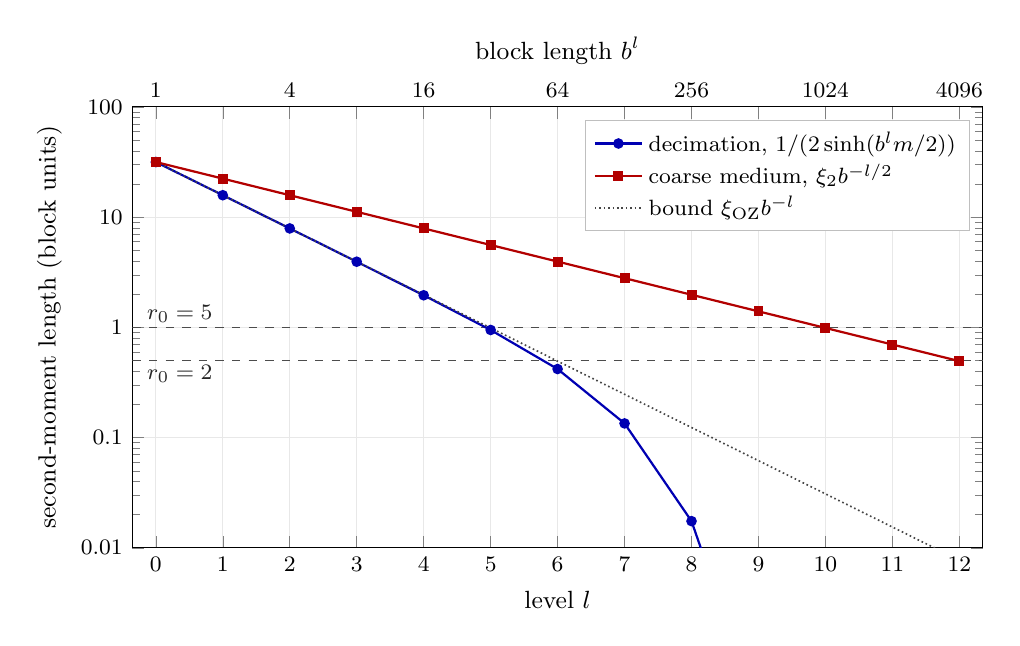
\begin{tikzpicture}
  \begin{semilogyaxis}[name=len, width=10.8cm, height=5.6cm, scale only axis,
      xmin=-0.35, xmax=12.35, ymin=0.01, ymax=100,
      xtick={0,...,12}, ytick={0.01,0.1,1,10,100}, log ticks with fixed point,
      grid=major, grid style={gray!18},
      xlabel={level $l$}, ylabel={second-moment length (block units)},
      every axis label/.style={font=\small}, tick label style={font=\footnotesize},
      legend style={font=\footnotesize, at={(0.985,0.97)}, anchor=north east, draw=gray!50, fill=white,
        cells={anchor=west}, row sep=-1pt}]
    \draw[gray!60!black, dashed] (axis cs:-0.35,1) -- (axis cs:12.35,1);
    \draw[gray!60!black, dashed] (axis cs:-0.35,0.5) -- (axis cs:12.35,0.5);
    \addplot[blue!70!black, thick, mark=*, mark size=1.5pt] coordinates {(0,31.6228) (1,15.8094) (2,7.90076)
      (3,3.94249) (4,1.95558) (5,0.947317) (6,0.418891) (7,0.134505) (8,0.0174705) (9,0.000305032)};
    \addlegendentry{decimation, $1/(2\sinh(b^lm/2))$}
    \addplot[red!70!black, thick, mark=square*, mark size=1.4pt] coordinates {(0,31.6228) (1,22.3607) (2,15.8114)
      (3,11.1803) (4,7.90569) (5,5.59017) (6,3.95285) (7,2.79508) (8,1.97642) (9,1.39754) (10,0.988212)
      (11,0.698771) (12,0.494106)};
    \addlegendentry{coarse medium, $\xi_2b^{-l/2}$}
    \addplot[gray!55!black, densely dotted, semithick] coordinates {(0,31.6241) (1,15.812) (2,7.90602) (3,3.95301)
      (4,1.97651) (5,0.988253) (6,0.494126) (7,0.247063) (8,0.123532) (9,0.0617658) (10,0.0308829)
      (11,0.0154415) (12,0.00772073)};
    \addlegendentry{bound $\xi_{\mathrm{OZ}}b^{-l}$}
    \node[font=\footnotesize, gray!30!black, anchor=south west, inner sep=1.5pt] at (axis cs:-0.2,1) {$r_0=5$};
    \node[font=\footnotesize, gray!30!black, anchor=north west, inner sep=1.5pt] at (axis cs:-0.2,0.5) {$r_0=2$};
  \end{semilogyaxis}
  \begin{axis}[at={(len.south west)}, anchor=south west, width=10.8cm, height=5.6cm, scale only axis,
      xmin=-0.35, xmax=12.35, ymin=0, ymax=1, axis x line*=top, axis y line=none,
      xtick={0,2,...,12}, xticklabels={$1$,$4$,$16$,$64$,$256$,$1024$,$4096$},
      xlabel={block length $b^l$},
      every axis label/.style={font=\small}, tick label style={font=\footnotesize}]
  \end{axis}
\end{tikzpicture}

  \caption{\textbf{Coarse second-moment lengths per level.} The nearest-neighbor precision on $\Z$ with $\varepsilon^\Pi/a^\Pi=10^{-3}$, for which $\cosh m=1+\varepsilon^\Pi/(2a^\Pi)$ gives $m=0.03162$ and $\xi_2=31.62$, is coarse-grained with block factor $b=2$; lengths are in units of the level-$l$ lattice, and the top axis gives the block length $b^l$. The exact law decimated $l$ times has the length $\xi^{(l)}_2=1/(2\sinh(b^lm/2))$ (\cref{thm:ren-decimation}), which follows the bound $\xi_{\mathrm{OZ}}b^{-l}$ of \cref{prop:ren-depth}(b) (dotted) while $b^lm\ll1$ and then falls exponentially. The coarse medium of blocks of side $b^l$ has the length $\xi_2b^{-l/2}$ (\cref{prop:ren-depth}(d)). The dashed lines are the thresholds $\frac12(r_0-1)^{1/2}$ of \cref{prop:ren-depth}(a) at $r_0=2$ and $r_0=5$: blocks of level $l+1$ reach contrast $r_0$ only while the length of level $l$ lies on or above them. The decimated length does so up to level $5$ for $r_0=2$ and up to level $4$ for $r_0=5$, block lengths $32$ and $16$ (\cref{chk:ren-depth}), within the bounds $b^l\le55.7$ and $b^l\le30.4$ of \cref{prop:ren-depth}(b); the coarse-medium length does so up to levels $11$ and $9$, block lengths $2048$ and $512$, within the bounds $b^l\le4000$ and $b^l\le1000$ of \cref{prop:ren-depth}(d).}
  \label{fig:ren-lengths}
\end{figure}

\subsection{Collectives across levels}\label{sec:ren-levels}

Which blocks of a hierarchy are collectives depends on the comparison medium of \cref{def:col-baseline}. For a population without declared geometry the comparison is exchangeable, and then only dense groups qualify.

For a finite closed population of $N$ agents with uniform leak and no declared geometry or coupling mechanism, the condition for a region of $n\ge2$ agents to be a collective at some admissible level is a pair of explicit inequalities, and each member of such a collective then has coupling to the other members above $\frac{(n-1)N}{n(N-1)}$ times the mean total coupling of an agent (Supplement, \cref{prop:ren-exchangeable}).

In a hierarchy, \cref{def:col-hierarchy} judges the blocks of level $l+1$ in the coarse medium of level $l$, against that medium's own comparison medium. For the nested medium, which declares no geometry at any level, the judgment has a closed form. Put $S_m=\sum_{j=1}^m\mathfrak q^{j-1}$, $M=b^m$ and
\[
\Delta_{\mathrm H}(b,\mathfrak q,m)=\frac b{b-1}-(S_m-1)-\frac M{M-1}S_m,\qquad T_{\mathrm H}(b,\mathfrak q,m)=\frac{MS_m(S_m-1)}{(M-1)\Delta_{\mathrm H}(b,\mathfrak q,m)}.
\]

In these terms, with the exchangeable comparison at every level, the level-$(l+1)$ blocks are collectives of the level-$l$ coarse medium, $0\le l\le n_{\mathrm H}-2$, if and only if $\Delta_{\mathrm H}(b,\mathfrak q,n_{\mathrm H}-l)>0$ and $\varepsilon^\Pi/(A_{\mathrm h}\mathfrak q^l)>T_{\mathrm H}(b,\mathfrak q,n_{\mathrm H}-l)$; nested collectives exist at every level if and only if $\mathfrak q<b/(2b^2-1)$ and the leak exceeds the largest of these thresholds, and at no level when $\mathfrak q\ge1/(2b-1)$ (Supplement, \cref{prop:ren-per-level}; \cref{fig:ren-per-level}).

\begin{figure}[!t]
  \centering
  % Figure: nested collectives judged level by level (prop:ren-per-level, thm:ren-nested), exchangeable comparison at
% every level. With S_m = sum_{j=1}^m q^{j-1}, M = b^m:
% Delta_H(b,q,m) = b/(b-1) - (S_m - 1) - M S_m/(M-1),  T_H(b,q,m) = M S_m (S_m - 1)/((M-1) Delta_H(b,q,m)).
% The level-(l+1) blocks are collectives of the level-l coarse medium iff Delta_H(b,q,n_H - l) > 0 and
% eps/(A_h q^l) > T_H(b,q,n_H - l) (prop:ren-per-level(b)).
% (a) The (b,q) plane, b in [2,5], logarithmic q axis; curves drawn through the integer values of b.
% Solid: q = b/(2b^2-1), the zero set of Delta_H at m = 2 (prop:ren-per-level(c): Delta_H > 0 for every m >= 2 iff
% q < b/(2b^2-1)). Dash-dotted: q = 1/(2b-1), the limit of the zero sets as m -> infinity, since
% Delta_H(b,q,m) = (2b-1)/(b-1) - 2/(1-q) + 2q^m/(1-q) - S_m/(b^m-1) tends to (2b-1)/(b-1) - 2/(1-q). On this curve
% Delta_H = 2q^m/(1-q) - S_m/(b^m-1) < 0 for every m >= 2: at m = 2 it equals -1/((2b-1)(b+1)); for m >= 3,
% S_m > 1 and (b-1)(2b-1)^{m-1} >= b^m. Delta_H decreases in q, so it is negative for every m above the curve and
% positive for all large m below it. Between the two curves the roots q_m(b) of Delta_H increase with m
% (q_2 = 0.2857, q_3 = 0.3062, q_8 = 0.3321, limit 1/3 for b = 2), so the levels with m = n_H - l large, the lower
% levels, qualify and the top level never does; prop:ren-per-level(f) proves that Delta_H increases strictly in
% m >= 2 for q < 1/(2b-1) and is negative for every m >= 2 for q >= 1/(2b-1). Dashed: q = 1/b (prop:ren-per-level(d): no level for q >= 1/b);
% the band 1/b < q < 1 is the power-law coherence of prop:abs-hierarchy(b). On 1789209 triples (b = 2..10,
% q = 0.001..0.999, m = 2..200) the sign pattern of Delta_H has no exception to these regions; the roots for
% m = 2..80 increase with m and stay below 1/(2b-1).
% Dot: the medium (b,q) = (2,0.2) of panel (b). Circles: the media (b,q) = (3,0.5), (2,0.7), (4,0.3) of
% chk:ren-per-level, in which no level qualified at any of 121 leaks in [1e-4,1e2].
% (b) (b,n_H,A_h,q) = (2,8,1,0.2): thresholds A_h q^l T_H(2,0.2,8-l) for l = 0..6 are 0.633645, 0.128496,
% 0.0264273, 0.00559337, 0.00125528, 3.17440e-4, 1.02400e-4 (T_H = 0.6336, 0.6425, 0.6607, 0.6992, 0.7845, 0.9920,
% 1.6000; Delta_H = 0.4951, ..., 0.2000). Bars: leaks at which the level-(l+1) blocks are collectives of the level-l
% coarse medium. Dashed: every level for eps > 0.633645, the binding level being l = 0. Recomputed from the explicit
% medium on 256 agents with coarse media Q Pi^(l) Q^T (sum convention, unit leak 2^l eps): lambda_2, cut per member
% and mean coupling equal the closed forms, the thresholds agree to 6.2e-11 relative, and on 121 leaks log-spaced in
% [1e-4,1e2] the first qualifying leak of each level is the first grid point above its threshold.
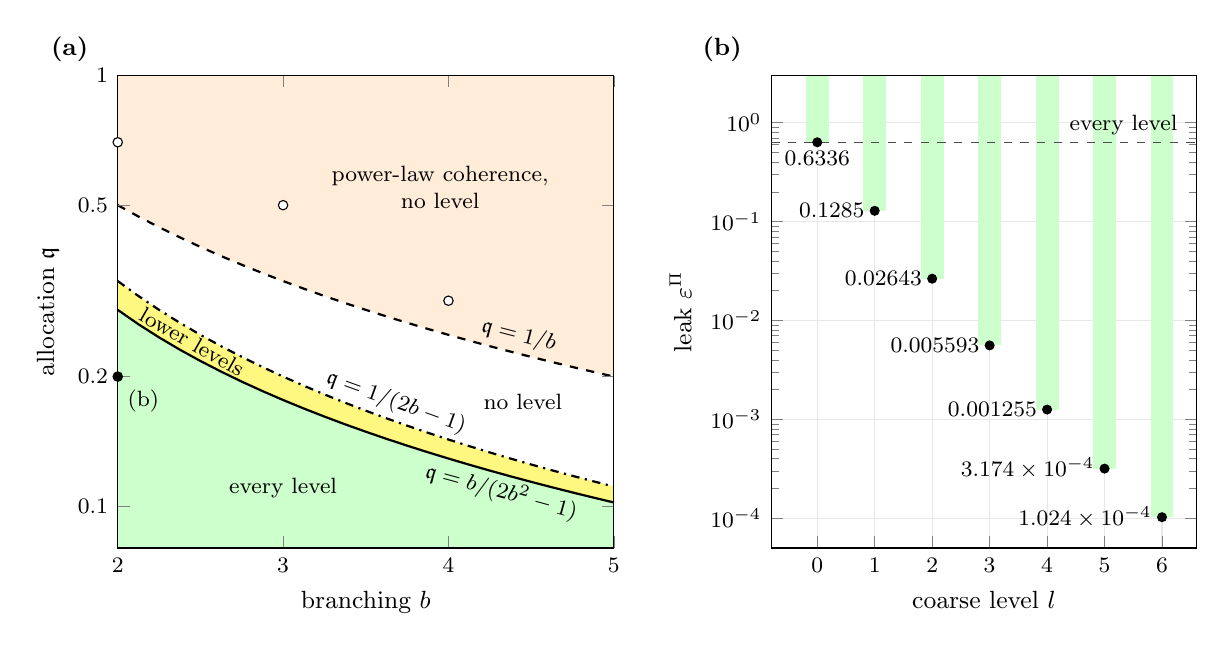
\begin{tikzpicture}
  \pgfplotsset{levelframe/.style={scale only axis, height=6.0cm,
      every axis label/.style={font=\small}, tick label style={font=\footnotesize}}}
  % panel (a): the (b, q) plane
  \begin{semilogyaxis}[levelframe, name=pa, width=6.3cm, xmin=2, xmax=5, ymin=0.08, ymax=1,
      xtick={2,...,5}, ytick={0.1,0.2,0.5,1}, log ticks with fixed point, axis on top, clip=false,
      xlabel={branching $b$}, ylabel={allocation $\mathfrak q$}]
    \addplot[draw=none, fill=green!20, forget plot] coordinates {(2,0.08) (2,0.285714) (2.125,0.264591) (2.25,0.246575) (2.375,0.231003) (2.5,0.217391) (2.625,0.205379)
      (2.75,0.19469) (2.875,0.185111) (3,0.176471) (3.125,0.168634) (3.25,0.161491) (3.375,0.15495) (3.5,0.148936)
      (3.625,0.143387) (3.75,0.138249) (3.875,0.133477) (4,0.129032) (4.125,0.124882) (4.25,0.120996) (4.375,0.117351)
      (4.5,0.113924) (4.625,0.110696) (4.75,0.107649) (4.875,0.104768) (5,0.102041) (5,0.08)} -- cycle;
    \addplot[draw=none, fill=yellow!50, forget plot] coordinates {(2,0.285714) (2.125,0.264591) (2.25,0.246575) (2.375,0.231003) (2.5,0.217391) (2.625,0.205379) (2.75,0.19469)
      (2.875,0.185111) (3,0.176471) (3.125,0.168634) (3.25,0.161491) (3.375,0.15495) (3.5,0.148936) (3.625,0.143387)
      (3.75,0.138249) (3.875,0.133477) (4,0.129032) (4.125,0.124882) (4.25,0.120996) (4.375,0.117351) (4.5,0.113924)
      (4.625,0.110696) (4.75,0.107649) (4.875,0.104768) (5,0.102041) (5,0.111111) (4.875,0.114286) (4.75,0.117647)
      (4.625,0.121212) (4.5,0.125) (4.375,0.129032) (4.25,0.133333) (4.125,0.137931) (4,0.142857) (3.875,0.148148)
      (3.75,0.153846) (3.625,0.16) (3.5,0.166667) (3.375,0.173913) (3.25,0.181818) (3.125,0.190476) (3,0.2)
      (2.875,0.210526) (2.75,0.222222) (2.625,0.235294) (2.5,0.25) (2.375,0.266667) (2.25,0.285714) (2.125,0.307692)
      (2,0.333333)} -- cycle;
    \addplot[draw=none, fill=orange!15, forget plot] coordinates {(2,0.5) (2.125,0.470588) (2.25,0.444444) (2.375,0.421053) (2.5,0.4) (2.625,0.380952) (2.75,0.363636)
      (2.875,0.347826) (3,0.333333) (3.125,0.32) (3.25,0.307692) (3.375,0.296296) (3.5,0.285714) (3.625,0.275862)
      (3.75,0.266667) (3.875,0.258065) (4,0.25) (4.125,0.242424) (4.25,0.235294) (4.375,0.228571) (4.5,0.222222)
      (4.625,0.216216) (4.75,0.210526) (4.875,0.205128) (5,0.2) (5,1) (2,1)} -- cycle;
    \addplot[black, thick] coordinates {(2,0.285714) (2.125,0.264591) (2.25,0.246575) (2.375,0.231003) (2.5,0.217391) (2.625,0.205379) (2.75,0.19469)
      (2.875,0.185111) (3,0.176471) (3.125,0.168634) (3.25,0.161491) (3.375,0.15495) (3.5,0.148936) (3.625,0.143387)
      (3.75,0.138249) (3.875,0.133477) (4,0.129032) (4.125,0.124882) (4.25,0.120996) (4.375,0.117351) (4.5,0.113924)
      (4.625,0.110696) (4.75,0.107649) (4.875,0.104768) (5,0.102041)};
    \addplot[black, thick, dashdotted] coordinates {(2,0.333333) (2.125,0.307692) (2.25,0.285714) (2.375,0.266667) (2.5,0.25) (2.625,0.235294) (2.75,0.222222)
      (2.875,0.210526) (3,0.2) (3.125,0.190476) (3.25,0.181818) (3.375,0.173913) (3.5,0.166667) (3.625,0.16)
      (3.75,0.153846) (3.875,0.148148) (4,0.142857) (4.125,0.137931) (4.25,0.133333) (4.375,0.129032) (4.5,0.125)
      (4.625,0.121212) (4.75,0.117647) (4.875,0.114286) (5,0.111111)};
    \addplot[black, thick, dashed] coordinates {(2,0.5) (2.125,0.470588) (2.25,0.444444) (2.375,0.421053) (2.5,0.4) (2.625,0.380952) (2.75,0.363636)
      (2.875,0.347826) (3,0.333333) (3.125,0.32) (3.25,0.307692) (3.375,0.296296) (3.5,0.285714) (3.625,0.275862)
      (3.75,0.266667) (3.875,0.258065) (4,0.25) (4.125,0.242424) (4.25,0.235294) (4.375,0.228571) (4.5,0.222222)
      (4.625,0.216216) (4.75,0.210526) (4.875,0.205128) (5,0.2)};
    % region labels
    \node[font=\footnotesize] at (axis cs:3.0,0.11) {every level};
    \path (axis cs:2.115,0.28491) -- node[sloped, font=\footnotesize, inner sep=0pt]
      {lower levels} (axis cs:2.785,0.203387);
    \node[font=\footnotesize] at (axis cs:4.45,0.175) {no level};
    \node[font=\footnotesize, align=center] at (axis cs:3.95,0.55) {power-law coherence,\\no level};
    % curve labels, along the curves
    \path (axis cs:3.95,0.130773) -- node[sloped, below, font=\footnotesize, inner sep=2pt]
      {$\mathfrak q=b/(2b^2-1)$} (axis cs:4.75,0.107649);
    \path (axis cs:3.3,0.178571) -- node[sloped, above, font=\footnotesize, inner sep=2pt]
      {$\mathfrak q=1/(2b-1)$} (axis cs:4.0,0.142857);
    \path (axis cs:4.1,0.243902) -- node[sloped, above, font=\footnotesize, inner sep=2pt]
      {$\mathfrak q=1/b$} (axis cs:4.7,0.212766);
    % media
    \addplot[only marks, mark=*, mark size=1.7pt, black] coordinates {(2,0.2)};
    \node[font=\footnotesize, anchor=north west, inner sep=1pt] at (axis cs:2.04,0.19) {(b)};
    \addplot[only marks, mark=*, mark size=1.7pt, black, mark options={fill=white}] coordinates {(3,0.5) (2,0.7)
      (4,0.3)};
  \end{semilogyaxis}
  \node[font=\small\bfseries, anchor=south east] at ($(pa.north west)+(-0.25cm,0.05cm)$) {(a)};
  % panel (b): leak thresholds per level
  \begin{semilogyaxis}[levelframe, name=pb, at={($(pa.south east)+(2.0cm,0)$)}, anchor=south west,
      width=5.4cm, xmin=-0.8, xmax=6.6, ymin=5e-5, ymax=3, xtick={0,...,6},
      ytick={1e-4,1e-3,1e-2,1e-1,1}, grid=major, grid style={gray!18},
      xlabel={coarse level $l$}, ylabel={leak $\varepsilon^\Pi$}]
    \fill[green!20] (axis cs:-0.2,0.633645) rectangle (axis cs:0.2,3);
    \fill[green!20] (axis cs:0.8,0.128496) rectangle (axis cs:1.2,3);
    \fill[green!20] (axis cs:1.8,0.0264273) rectangle (axis cs:2.2,3);
    \fill[green!20] (axis cs:2.8,0.00559337) rectangle (axis cs:3.2,3);
    \fill[green!20] (axis cs:3.8,0.00125528) rectangle (axis cs:4.2,3);
    \fill[green!20] (axis cs:4.8,0.00031744) rectangle (axis cs:5.2,3);
    \fill[green!20] (axis cs:5.8,0.0001024) rectangle (axis cs:6.2,3);
    \draw[gray!60!black, dashed] (axis cs:-0.8,0.633645) -- (axis cs:6.6,0.633645);
    \addplot[only marks, mark=*, mark size=1.6pt, black] coordinates {(0,0.633645) (1,0.128496)
      (2,0.0264273) (3,0.00559337) (4,0.00125528) (5,0.00031744) (6,0.0001024)};
    \node[font=\footnotesize, anchor=north, inner sep=3pt] at (axis cs:0,0.633645) {$0.6336$};
    \node[font=\footnotesize, anchor=east, inner sep=3.5pt] at (axis cs:1,0.128496) {$0.1285$};
    \node[font=\footnotesize, anchor=east, inner sep=3.5pt] at (axis cs:2,0.0264273) {$0.02643$};
    \node[font=\footnotesize, anchor=east, inner sep=3.5pt] at (axis cs:3,0.00559337) {$0.005593$};
    \node[font=\footnotesize, anchor=east, inner sep=3.5pt] at (axis cs:4,0.00125528) {$0.001255$};
    \node[font=\footnotesize, anchor=east, inner sep=3.5pt] at (axis cs:5,0.00031744) {$3.174\times10^{-4}$};
    \node[font=\footnotesize, anchor=east, inner sep=3.5pt] at (axis cs:6,0.0001024) {$1.024\times10^{-4}$};
    \node[font=\footnotesize, anchor=south east, inner sep=1.5pt] at (axis cs:6.35,0.68) {every level};
  \end{semilogyaxis}
  \node[font=\small\bfseries, anchor=south east] at ($(pb.north west)+(-0.25cm,0.05cm)$) {(b)};
\end{tikzpicture}

  \caption{\textbf{Nested collectives judged level by level.} The nested medium of \cref{thm:ren-nested} with the exchangeable comparison at every level (Supplement, \cref{prop:ren-per-level}). (a) The plane of the branching $b$ and the allocation $\mathfrak q$, with the curves drawn through the integer values of $b$. Below the solid curve $\mathfrak q=b/(2b^2-1)$, $\Delta_{\mathrm H}(b,\mathfrak q,m)>0$ for every $m\ge2$, and the blocks of every level are collectives above a leak threshold (\cref{prop:ren-per-level}(c)). The dash-dotted curve $\mathfrak q=1/(2b-1)$ is the limit of the zero sets of $\Delta_{\mathrm H}(b,\mathfrak q,m)$ as $m\to\infty$. Between the two curves $\Delta_{\mathrm H}(b,\mathfrak q,2)\le0$ while $\Delta_{\mathrm H}(b,\mathfrak q,m)$ increases with $m$ and is positive for all large $m$, so the top level is never a collective and the lower levels of a deep enough hierarchy are, above a leak threshold; above the dash-dotted curve $\Delta_{\mathrm H}<0$ for every $m$, and no level is (\cref{prop:ren-per-level}(f)). This includes the range $\mathfrak q\ge1/b$ of \cref{prop:ren-per-level}(d) (dashed curve), where \cref{prop:abs-hierarchy}(b) gives power-law coherence for $\mathfrak q<1$. The dot marks the medium of panel (b), and the circles the media $(b,\mathfrak q)=(3,0.5)$, $(2,0.7)$ and $(4,0.3)$ of \cref{chk:ren-per-level}, in which no level qualified at any of $121$ leaks in $[10^{-4},10^2]$. (b) For $(b,n_{\mathrm H},A_{\mathrm h},\mathfrak q)=(2,8,1,0.2)$ the level-$(l+1)$ blocks are collectives of the level-$l$ coarse medium at the leaks above $A_{\mathrm h}\mathfrak q^lT_{\mathrm H}(b,\mathfrak q,n_{\mathrm H}-l)$ (bars), whose values for $l=0,\dots,6$ are $0.6336$, $0.1285$, $0.02643$, $0.005593$, $0.001255$, $3.174\times10^{-4}$ and $1.024\times10^{-4}$; they fall like $\mathfrak q^l$, while $T_{\mathrm H}$ rises from $0.634$ at $l=0$ to $1.6$ at $l=6$. The largest, at $l=0$, is the leak $0.6336$ above which collectives exist at every level (dashed line).}
  \label{fig:ren-per-level}
\end{figure}

\subsection{Memory and the adiabatic reduction}\label{sec:ren-memory}

\Cref{thm:agy-closure-average} treats one collective with its exterior held fixed. A coarse-grained population is a set of blocks whose exteriors are the other blocks, so we need the joint version. Let $\varpi_1\le\varpi_2\le\cdots$ be the eigenvalues of $\Pi$, let $\mathsf V_{\mathrm s}$ and $\mathsf V_{\mathrm f}$ hold orthonormal eigenvectors of the $M$ smallest and of the others, let $\varkappa_\Phi=\lambda_{\max}(\Pi_\Phi)$, and put $\mathsf t_\Theta=\Vert\Pi_{\perp\Phi}\Vert/(\varkappa_\perp-\varkappa_\Phi)$.

\begin{theorem}[Exact reduction of a partitioned reversible population]\label{thm:ren-memory}
Let $\Pi\succ0$ be symmetric, let $x$ follow $\mathrm dx=-\Pi x\mathrm dt+\sqrt2\mathrm d\mathsf B_t$ in its stationary law, let $\Phi\in\R^{N\times M}$ have orthonormal columns, and let $y=\Phi^\top x$.
\begin{enumerate}
\item[(a)] (Static law.) $\Cov(y)^{-1}=\Pi_\Phi-\mathcal D$, with $\mathcal D$ as in \cref{lem:ren-galerkin}.
\item[(b)] (Memory.) $\dot y(t)=-\Pi_\Phi y(t)+\int_0^t\Gamma(t-t')y(t')\mathrm dt'+\mathfrak f(t)$, with kernel $\Gamma(u)=\Pi_{\perp\Phi}^\top e^{-\Pi_{\perp\perp}u}\Pi_{\perp\Phi}\succeq0$, $\Vert\Gamma(u)\Vert\le\Vert\Pi_{\perp\Phi}\Vert^2e^{-\varkappa_\perp u}$ and $\int_0^\infty\Gamma(u)\mathrm du=\mathcal D$: the static correction of the bridge theorem is the integrated memory kernel.
\item[(c)] (Slow and fast parts.) If $\varkappa_\perp>\varkappa_\Phi$, then $\varpi_M\le\varkappa_\Phi<\varkappa_\perp\le\varpi_{M+1}$, and the largest principal angle $\Theta$ between $\operatorname{range}\Phi$ and $\operatorname{range}\mathsf V_{\mathrm s}$ satisfies $\sin\Theta\le\mathsf t_\Theta$. If $\mathsf t_\Theta<1$, then exactly $y=\mathsf Tz_{\mathrm s}+y_{\mathrm f}$, where $z_{\mathrm s}=\mathsf V_{\mathrm s}^\top x$ is an Ornstein--Uhlenbeck process with drift $\diag(\varpi_1,\dots,\varpi_M)$, $\mathsf T=\Phi^\top\mathsf V_{\mathrm s}$ is invertible, and $y_{\mathrm f}$ is independent of $z_{\mathrm s}$, has an autocovariance that decays at rates at least $\varkappa_\perp$, and has relative weight $\Vert\Cov(y)^{-1/2}\Cov(y_{\mathrm f})\Cov(y)^{-1/2}\Vert\le\mathsf t_\Theta^2\varkappa_\Phi/\varkappa_\perp$. The slow part is exactly Markov, with drift $\mathsf T\diag(\varpi_1,\dots,\varpi_M)\mathsf T^{-1}$, which differs from $\Pi_\Phi$ by at most $\Vert\Pi_{\perp\Phi}\Vert\mathsf t_\Theta/(1-\mathsf t_\Theta^2)^{1/2}$ in norm.
\item[(d)] (Contrast.) For the block indicators of a partition into regions $C_1,\dots,C_M$ of a diffusive $\Pi$, whose leaks need not be uniform, $\varkappa_\perp\ge\xin^{\min}$, the minimum of $\xin(C_j)$ over the regions with at least two members (the bounds are vacuous if every region is a singleton), $\varkappa_\Phi\le\max_j(2\xout(C_j)-\bar\varepsilon_{C_j})$, which for uniform leak $\varepsilon^\Pi$ is $2\xout^{\max}-\varepsilon^\Pi$ with $\xout^{\max}=\max_j\xout(C_j)$, and $\Vert\Pi_{\perp\Phi}\Vert\le\sigma_{\mathrm{cut}}$. If $\xin^{\min}>\max_j(2\xout(C_j)-\bar\varepsilon_{C_j})$, every bound of (a) to (c) holds with $\varkappa_\perp-\varkappa_\Phi\ge\xin^{\min}-\max_j(2\xout(C_j)-\bar\varepsilon_{C_j})$, which for uniform leak is $\xin^{\min}-2\xout^{\max}+\varepsilon^\Pi$. If all blocks have the same rates $\xin$ and $\xout$, with contrast $r>2$, the relative fast weight is at most $2(\Vert\Pi_{\perp\Phi}\Vert/(\xout(r-2)))^2/r$.
\end{enumerate}
\end{theorem}
% src: H4-T8 (CHECKED); C3_05 recomputation (200 populations)
Proof in \cref{app:ren}; checked on $200$ random partitioned populations and on block media of square blocks (\cref{chk:ren-memory}). Part (d) is the multi-block form of the closure bound of \cref{thm:agy-h1}. Coarse-graining along collectives with $\Vert\Pi_{\perp\Phi}\Vert^2\ll\xin^{\min}\xout$ makes memory a correction of that relative order; coarse-graining across them does not. The spectral norm is the intensive measure: for $M$ identical blocks $\sigma^2_{\mathrm{cut}}$ grows in proportion to $M$, while $\Vert\Pi_{\perp\Phi}\Vert$ and $\Vert\mathcal D\Vert$ do not (\cref{chk:ren-memory}).

The adiabatic reduction of \citet{friston2019free}, read in its primary text, builds scales with two operators. A grouping operator $G$ forms a particular partition into particles from the coupling structure of the Jacobian and eliminates internal states by conditioning on blankets, absorbing their fluctuations into those of the next level; a reduction operator $R$ keeps the slow eigenmodes of each particle's own blanket Jacobian as the states of the next level and absorbs the fast ones into fluctuations. An ensemble assumption takes the slow and fast modes of different particles to be uncoupled, correlations among the induced fluctuations are set aside, and $R\circ G$ is read as a renormalization that preserves the functional form of the dynamics, with slower modes and smaller fluctuations at each level. The linear reversible analogue of $R$ is a frame of per-particle slowest modes.

\begin{proposition}[Per-particle slow modes]\label{prop:ren-perron}
In the setting of \cref{thm:ren-memory}, let a partition into particles $C_1,\dots,C_M$ be given, let $\mathsf u_j$ be a unit eigenvector of the smallest eigenvalue of $\Pi_{C_jC_j}$, the slowest mode of particle $j$'s own drift, which is positive by the Perron--Frobenius theorem when $\Pi$ is diffusive and $C_j$ is connected, and let $\Phi^{\mathsf P}=\diag(\mathsf u_1,\dots,\mathsf u_M)$. The reduction AR0, $\mathrm dy=-\Pi_{\Phi^{\mathsf P}}y\mathrm dt+\sqrt2\mathrm d\mathsf W_t$ with $\mathsf W$ a standard Brownian motion, discards the fast modes.
\begin{enumerate}
\item[(a)] AR0 is exact, in law and in dynamics, if and only if $\Pi_{C_kC_j}\mathsf u_j\in\operatorname{span}\mathsf u_k$ for all $j\neq k$: the slow mode of each particle drives the other particles only along their slow modes. This is the ensemble assumption in linear form; within a particle it holds automatically.
\item[(b)] Otherwise the stationary precision of AR0 errs by exactly $\mathcal D^{\mathsf P}$, the matrix $\mathcal D$ of the frame $\Phi^{\mathsf P}$, and \cref{thm:ren-memory} applies with $\Vert\Pi_{\perp\Phi^{\mathsf P}}\Vert$, which collects only couplings from the slow mode of one particle to fast modes of others. The Markov reduction that matches the stationary law and the short-time derivative of the autocovariance of $y$ has drift $\Pi_{\Phi^{\mathsf P}}-\mathcal D^{\mathsf P}$ and unit noise; its only error is the memory of \cref{thm:ren-memory}(b).
\item[(c)] Per-particle modes miss the global slow mode: with uniform leak the slowest mode $\one/N^{1/2}$, of rate $\varepsilon^\Pi$, lies in the span of the block indicators but not in $\operatorname{range}\Phi^{\mathsf P}$ unless every $\mathsf u_j$ is constant. If $\varkappa_\perp$, computed in the frame $\Phi^{\mathsf P}$, exceeds $\lambda_{\min}(\Pi_{\Phi^{\mathsf P}})$, then $0\le\lambda_{\min}(\Pi_{\Phi^{\mathsf P}})-\varepsilon^\Pi\le\Vert\Pi_{\perp\Phi^{\mathsf P}}\Vert^2/(\varkappa_\perp-\lambda_{\min}(\Pi_{\Phi^{\mathsf P}}))$, while $\lambda_{\min}(\Pi_\Phi)=\varepsilon^\Pi$ exactly for block averages.
\item[(d)] For equal blocks, $M^{-1}\tr\Pi_\Phi=N^{-1}\sum_i(\varepsilon^\Pi_i+a^\partial_i)\le N^{-1}\tr\Pi$, with $a^\partial_i$ the coupling of agent $i$ to other blocks, and $\tr(\Pi_\Phi-\mathcal D)\le\tr\Pi_\Phi$: block averages are slower on average. Whether fluctuations become smaller depends on the normalization: block averages have variance at most $\lambda_{\max}(\Sigma)/\lvert X\rvert$, while the normalization that keeps the coarse coupling fixed leaves the noise intensity unchanged.
\end{enumerate}
\end{proposition}
% src: H4-P9 (CHECKED); C3_05 recomputation; H4-R2 and H1-R1 merged on the operators per HC_critic Section 4 (G eliminates, R keeps slow eigenmodes)
Proof in \cref{app:ren}; checked on block media in \cref{chk:ren-perron}, where at contrast $35.1$ the Perron frame couples the particles more weakly than the frame of block averages, but its slowest retained rate is $1.0368\times10^{-3}$ against the exact $10^{-3}$. Without contrast the Galerkin description fails at leading order.

For the nearest-neighbor precision on $\Z$ and blocks of $b$ sites the coarse medium overstates the squared second-moment length of the block averages, in block units, by a factor that tends to $b$ as the leak vanishes, and averaged update weights overstate the coarse message weight by the same factor up to corrections of order the leak (Supplement, \cref{ex:ren-no-contrast}).

The grouping step $G$, the elimination of internal states, drops a memory kernel, an initial-state term and the color of the force from an exact equation for the retained states, those that are not internal, which are Markov with a transition law independent of the initial law if and only if no retained state is driven by an internal one (Supplement, \cref{prop:ren-adiabatic}, for stable linear dynamics on a particular partition, under the hypotheses stated there). The size of what is dropped is a numerical observation without a proved rate (\cref{obs:ren-adiabatic-rate}), and \cref{rem:ren-rgm} compares renormalizing generative models.

\subsection{The framework under coarse-graining}\label{sec:ren-closure}

Codes, relay ranks, decision dimensions and interpretation levels under aggregation are treated in the Supplement (\cref{sec:ren-codes}). A meta-agent $J$ that aggregates the public messages of its members with weights $\mathsf w_j\ge0$ that sum to one has the aggregate code $T_c\bar U_J$, with $\bar U_J=\sum_{j\in J}\mathsf w_jU_j$. Aggregation in public coordinates never raises the rank of a code, and aggregation after true translation loses nothing (\cref{prop:ren-codes,prop:ren-code-levels}); under the hypotheses stated there, the effective rank of stationary averaged relays is nonincreasing along the relay and the Hayek dimension is nonincreasing up the hierarchy (\cref{prop:ren-relay-rank,prop:ren-hayek}); and literal reading in a regular hierarchy counts the common prior once per agent in the limit of many rounds, while consensus on information contributions that passes exact sums upward and adds the common prior once at the top returns the union posterior (\cref{prop:ren-literal-levels}).

For networks without coordinates the Supplement (\cref{sec:ren-network}) compares contrast with the Laplacian renormalization group of \citet{villegas2023laplacian}. With uniform leak that procedure does not depend on the leak, whereas contrast does (\cref{prop:ren-lrg}); the two agree on an interval of leaks for a population formed by two blocks of equal size with an equitable cut and equal internal gaps, under the gap condition stated there (\cref{prop:ren-lrg-agreement}); in an example with interleaved scales no single diffusion time returns every set that contrast selects (\cref{ex:ren-interleaved}); and which regions of high ratio the procedure returns is an open problem (\cref{conj:ren-lrg}).

\begin{theorem}[What coarse-graining preserves]\label{thm:ren-closure}
Let a population satisfy \cref{asm:ren-standing}, and let a partition $\mathcal X$ into blocks, the candidate meta-agents, be coarse-grained by block averaging.
\begin{enumerate}
\item[(a)] (Static law.) The block coordinates have the Gaussian precision $\Pi_\Phi-\mathcal D$ (\cref{lem:ren-galerkin}); whether or not the leak is uniform, $\Vert\mathcal D\Vert\le\Vert\Pi_{\perp\Phi}\Vert^2/\xin^{\min}\le\sigma^2_{\mathrm{cut}}/\xin^{\min}$ and $\lvert\mathcal D_{XY}\rvert\le\sigma_X\sigma_Y/\xin^{\min}$, with $\xin^{\min}$ the minimum of $\xin(X)$ over the blocks with at least two members (the bounds are vacuous if every block is a singleton), and these bound the departure from $\Pi_\Phi$ of the exact law, which is in general not diffusive (\cref{ex:ren-block-average}). For uniform leak $\mathcal D$ also leaves the leak unchanged (\cref{lem:ren-galerkin}(c)).
\item[(b)] (Coarse level-0 network.) Under $e(t+1)=We(t)+\zeta(t)$ the block averages obey $\bar e(t+1)=W^{(1)}\bar e(t)+\diag(\lvert X\rvert)^{-1}\mathsf PWe_\perp(t)+\bar\zeta(t)$, with $e_\perp=e-\mathsf P^\top\bar e$ and $W^{(1)}=\diag(\lvert X\rvert)^{-1}\mathsf PW\mathsf P^\top$, whose entry $W^{(1)}_{XY}$ is the mean total weight that a member of $X$ places on $Y$. The matrix $W^{(1)}$ is nonnegative if $W$ is, and its row sums are block means of row sums, so the coarse leak is the mean leak and \textup{(C$_r$)} and \textup{(M)} are inherited; if the local noises satisfy \textup{(B)} of \cref{asm:sca-standing}, the $\bar\zeta_X$ are independent, with variance at most $q/\lvert X\rvert$, and equal to $q/\lvert X\rvert$ when every local noise has variance $q$. The memory term vanishes for every $e_\perp$ if and only if the partition is lumpable for $W$ (\cref{def:met-lumpable}), and then the coarse population is exactly a level-0 network; otherwise the exact reduction is \cref{thm:agy-mori-zwanzig}, with the bounds of \cref{thm:ren-memory} in continuous time and, for one coordinate of a reversible recursion, of \cref{lem:met-discrete-closure}.
\item[(c)] (Contrast between meta-agents.) For blocks of equal size and uniform leak, every set $S$ of at least two blocks has coarse contrast $r^{(1)}(S)\ge r(\bigcup S)$, with equality if and only if a slowest internal mode of $\bigcup S$ is constant on blocks, as at every level of the nested medium (\cref{thm:ren-nested}(c)). Hence if $\bigcup S$ is a collective of the fine medium at level $r_0$, then $S$ is a collective of the coarse medium at the same level whenever $r_0$ exceeds the coarse baseline $\bar r^{(1)}_{\mathrm{hom}}$ (\cref{def:col-hierarchy}). Under the exchangeable clause at both levels, with $N$ agents in blocks of $s$, $\bar r^{(1)}_{\mathrm{hom}}-1=\frac{N-1}{N-s}\cdot\frac{\bar c}{\bar d}(\bar r_{\mathrm{hom}}-1)$, with $\bar d$ the mean total coupling of an agent and $\bar c$ its mean coupling to other blocks, so the coarse baseline is the lower one exactly when $\bar c/\bar d\le(N-s)/(N-1)$.
\item[(d)] (Codes and interpretation.) Codes and interpretation levels transform as in \cref{prop:ren-codes,prop:ren-code-levels,prop:ren-literal-levels}: aggregation after true translation preserves codes, and the information form is closed while literal reading compounds.
\item[(e)] (Records.) In the record model of \cref{def:fw-record-model} the record equation closes exactly for block averages, $\bar z_{k,X}(t+1)=\omega_k\bar e_X(t)+(1-\omega_k-\delta_k)\bar z_{k,X}(t)+\bar\zeta^z_{k,X}(t)$, so $\beta_k$, $\omega_k$, $\delta_k$ and $\upsilon_k$ do not renormalize and record noise becomes $q_z/\lvert X\rvert$; the read term closes exactly for local records ($\ell_{r,k}=0$) and, at range, on record fields constant on blocks, with the kernel $\mathsf K^{(1)}_k(X,Y)=\lvert X\rvert^{-1}\sum_{x\in X,y\in Y}\mathsf K_k(x-y)$, a Galerkin projection otherwise; the message term keeps the memory of (b). On $\Z^D$ with cubic blocks the reduced model of the mean mode (\cref{prop:sca-records}), hence $\varepsilon_{\mathrm{rec}}$ and the correlation time of the collective mean, is the same at every level.
\item[(f)] (What fails.) Without contrast the Markov coarse coupling and squared length are wrong by the block factor $b$, up to corrections that vanish with the leak (\cref{ex:ren-no-contrast}); contrast is computed in the coarse medium, with the error of (a), because the exact law leaves the diffusive class (\cref{ex:ren-block-average}); for directed attention, discrete-time closure beyond \cref{lem:met-discrete-closure} is open, and contrast is undefined where the precision is not diffusive (\cref{open:col-non-diffusive}); without declared geometry collectives must be denser than average, and nested collectives at every level need $\mathfrak q<b/(2b^2-1)$, a leak above an explicit threshold and a declared level for each level (\cref{prop:ren-exchangeable,prop:ren-per-level}).
\end{enumerate}
\end{theorem}
% src: H4-T18 (DERIVED; parts CHECKED as cited), with (3) restated per H6-P12 and generalized here to equal blocks without equitability (checked by ren_checks.py part D), (6)(iv) replaced per H6-T2, the closure condition of (2) unified with def:met-lumpable per HC_critic V6
Proof in \cref{app:ren}; part (c) is checked on random populations with blocks that are not equitable (\cref{chk:ren-closure}), and \cref{tab:ren-parameters} lists how each parameter transforms. The framework is closed under coarse-graining exactly for partitions whose span of block indicators the precision leaves invariant, as in the nested medium; approximately, with the averaged-weight coarse parameters in error by relative order $\Vert\Pi_{\perp\Phi}\Vert^2/(\xin^{\min}\xout)$, when that ratio is small; and not even approximately for blocks without contrast. High contrast alone does not make the ratio small: for uniform leak $\sigma_X^2\le2d_{\max}(X)(\xout(X)-\varepsilon^\Pi)$ (\cref{lem:ren-galerkin}(b)), so that $\sigma_X^2/(\xin^{\min}\xout(X))\le2d_{\max}(X)/\xin^{\min}$, and this per-block ratio is small when every agent's coupling across the boundary is small against $\xin^{\min}$, as at high contrast when the cut is spread over the members; the bound gives a sufficient condition for that ratio, not a necessary one. Two cliques joined by a single strong edge have contrast that grows without bound with their size while the exact coarse coupling stays near half the averaged one (\cref{chk:ren-memory}); what survives there is the Markov property of the slow part, by \cref{thm:ren-memory}(c), with a drift that differs from $\Pi_\Phi$ at order one.

\begin{table}[t]
\centering
\caption{Parameters of the framework under block averaging (\cref{thm:ren-closure}). Lengths are in block units.}
\label{tab:ren-parameters}
\begin{tabular}{@{}p{0.25\textwidth}p{0.43\textwidth}p{0.24\textwidth}@{}}
\toprule
Parameter & Coarse value & Status\\
\midrule
uniform leak $\varepsilon$ & unchanged per base round; $b^2\varepsilon$ per coarse round of $b^2$ base rounds & exact; rescaling (\cref{prop:ren-exponents})\\
precision couplings & $\cut(X,Y)$ in the coarse medium, corrected by $\mathcal D$ & exact; $\Vert\mathcal D\Vert\le\Vert\Pi_{\perp\Phi}\Vert^2/\xin^{\min}$\\
message weights $W_{ij}$ & $W^{(1)}_{XY}$, mean total weight of a member of $X$ on $Y$ & exact if lumpable; memory otherwise\\
axis rate, $a/\varepsilon$ & rate times $b$; $a/\varepsilon$ divided by about $b^2$ & exact flow (\cref{thm:ren-flows})\\
second-moment length & divided by $b$, up to a constant & exact formula (\cref{thm:ren-flows})\\
local noise $q$ & $q/\lvert X\rvert$ & equality for equal variances; an upper bound under \textup{(B)}\\
codes $H_j$ & $T_c\bar U_X$ (public); unchanged (translated) & exact\\
record parameters & $\beta_k,\omega_k,\delta_k,\upsilon_k$ unchanged; noise $q_z/\lvert X\rvert$; kernel averaged & exact; Galerkin at range\\
interpretation level & literal: overcounting multiplies; information form: closed & exact (regular hierarchies)\\
contrast & $r^{(1)}(S)\ge r(\bigcup S)$ for equal blocks & exact inequality\\
memory & kernel at most $\Vert\Pi_{\perp\Phi}\Vert^2e^{-\xin^{\min}u}$, integral $\mathcal D$ & exact bounds\\
\bottomrule
\end{tabular}
\end{table}

Open problems beyond the exact cases, among them contrast for the non-diffusive laws of block averages and discrete-time closure for non-reversible updates, are listed in the Supplement (\cref{open:ren-beyond}).

% Section 14: Abstract environments and selective sensing (key env)
% src: H5 (all) as repaired by critic V11, V12 and Sections 2.2, 2.3, 2.6, 2.7; H1 Section 6 (H1-R26, H1-R27) at its reading levels; H3-E2, H3-E3 by reference to sec:met
\section{Abstract environments and selective sensing}\label{sec:env}

The author's fifth idea gives meta-agents external states of their own: a corporation senses an informational environment of prices and indices rather than a physical medium, people sense the economy, and nerve cells sense chemical potentials but not gravity. \Cref{sec:met} declares a meta-agent's external states as linear functions of the joint process and asks when they have closed dynamics. This section treats, in linear-Gaussian exteriors, the prior question of part H5c of hypothesis H5 for an agent at any level, which functions of its exterior it should sense, by stating what a sensor optimal for a declared horizon-$h$ predictive-information objective reads (\cref{def:env-attention-objective}); the one-step expected free energy of the framework does not imply this objective and can oppose it (\cref{rem:env-efe-horizon-free,rem:env-two-step}). Sensors with a fixed number of channels or a Shannon budget that carry most information about the exterior at a horizon read the leading canonical variates between present and future (\cref{thm:env-canonical}); the horizon decides how many and which (\cref{prop:env-horizon,prop:env-diffusive}); preferences and control select within this order and can reverse it (\cref{thm:env-control,ex:env-fast-preference}). A selection principle of coupling, predictability and relevance (\cref{prop:env-selection}) turns the nerve cell into a model in which gravity fails the coupling clause by more than thirteen orders of magnitude per single-particle reading, and by nearly ten at equal pooling of molecular samples (\cref{ex:env-cell}). Aggregates of many agents are closed environments when the population consists of interchangeable types and carry memory otherwise (\cref{prop:env-aggregate-closure,prop:env-aggregate-memory}), and long-horizon decisions need few of them (\cref{thm:env-hayek-horizon,ex:env-firm,ex:env-person}). The main text states the sensor theorem, the dependence on the horizon, the control theorem and the Hayek dimension at a horizon; the lemma on summaries of the past, the diffusive case, the remarks on expected free energy, the selection principle with the cell model, the closure and memory of aggregates, the worked firm and person, sensing across levels and memberships, and the open problems are in the Supplement.

Theorems are for linear-Gaussian models. The exterior is a stationary Gauss--Markov process $\eta_{t+1}=F\eta_t+w_t$ with $\rho(F)<1$ and $Q\succ0$, so that every canonical correlation between $\eta_t$ and $\eta_{t+h}$ is below one; for the exterior's own dynamics this is the spectral contraction (C$_\rho$) with the stationary moment bound (M) of \cref{asm:sca-standing}, on which every correlation time below is conditional. Sensors are linear with Gaussian noise independent of everything else. The capacity of a sensor is either its number $\kappa$ of scalar channels, the attention capacity of \cref{def:fw-system} measured in channels, or its Shannon information $I(s;\eta_t)$ in nats, bounded by a budget $I_{\max}$. The horizon $h\ge1$ is a fixed number of rounds. For a matrix $X$, $\sigma_{\mathsf j}(X)$ is its $\mathsf j$-th largest singular value and $\lambda_{\mathsf j}(X)$ its $\mathsf j$-th eigenvalue, in decreasing order for symmetric matrices and by decreasing modulus otherwise. The $\mathsf u_{\mathsf j}$ are left eigenvectors of $F$, the mode amplitudes are $\mathsf u_{\mathsf j}^\top\eta$, and $\tau_{\mathsf j}=-1/\ln\lvert\lambda_{\mathsf j}(F)\rvert$ is the correlation time of mode $\mathsf j$.

\subsection{Linear sensors and canonical variates}\label{sec:env-sensors}

\begin{definition}[Linear sensors and canonical variates]\label{def:env-sensor}
Let $\mathsf X\in\R^{d_{\mathsf X}}$, what a sensor can read, and $\mathsf Y\in\R^{d_{\mathsf Y}}$, what is to be predicted, be jointly Gaussian with mean zero, covariances $\Sigma_{\mathsf X}\succ0$ and $\Sigma_{\mathsf Y}\succ0$ and cross-covariance $\Sigma_{\mathsf X\mathsf Y}$. The canonical correlations $1\ge\sigma_1\ge\sigma_2\ge\dots$ are the singular values of the whitened cross-covariance $\mathsf C=\Sigma_{\mathsf X}^{-1/2}\Sigma_{\mathsf X\mathsf Y}\Sigma_{\mathsf Y}^{-1/2}$, padded with zeros to length $d_{\mathsf X}$, and $\sigma_{\mathsf j}=0$ for $\mathsf j>d_{\mathsf X}$; with orthonormal left singular vectors $\mathsf e_{\mathsf j}$, the canonical variates $\mathsf e_{\mathsf j}^\top\Sigma_{\mathsf X}^{-1/2}\mathsf X$ are uncorrelated with unit variance \citep{hotelling1936relations}. A sensor with $\kappa$ channels is $s=H\mathsf X+v$, with $H\in\R^{\kappa\times d_{\mathsf X}}$ and $v\sim\Ncal(0,I_\kappa)$ independent of $(\mathsf X,\mathsf Y)$; a noise covariance $R\succ0$ reduces to this form by $s\mapsto R^{-1/2}s$. With the whitened sensor $\tilde H=H\Sigma_{\mathsf X}^{1/2}$, its captured covariance is
\[
\mathsf G_s=\tilde H^\top\bigl(I_\kappa+\tilde H\tilde H^\top\bigr)^{-1}\tilde H,
\]
whose eigenvalues $\mathsf g_1\ge\mathsf g_2\ge\dots$, the captured fractions, lie in $[0,1)$, at most $\kappa$ of them positive. When $\kappa>d_{\mathsf X}$ we put $\mathsf g_{\mathsf j}=0$ for $\mathsf j>d_{\mathsf X}$, and likewise $\lambda_{\mathsf j}(\mathsf J)=0$ for $\mathsf j>d_{\mathsf X}$ when $\mathsf J\succeq0$ is a symmetric $d_{\mathsf X}\times d_{\mathsf X}$ matrix, so that a channel beyond the $d_{\mathsf X}$-th carries noise only. The sensor reads the variate $f^\top\Sigma_{\mathsf X}^{-1/2}\mathsf X$ with captured fraction $\mathsf g>0$ when $\mathsf G_sf=\mathsf gf$ and $\lvert f\rvert=1$. A noiseless sensor $s=H\mathsf X$ of rank $\kappa$ has as captured covariance the orthogonal projector onto the row space of $\tilde H$.
\end{definition}
% src: H5-D1 (captured covariance renamed G_s, critic 2.7)

\begin{lemma}[Information and error of a linear sensor]\label{lem:env-information}
In the setting of \cref{def:env-sensor}:
\begin{enumerate}
\item[(i)] $\Cov(\Sigma_{\mathsf X}^{-1/2}\mathsf X\mid s)=I-\mathsf G_s$ and $I(s;\mathsf X)=-\frac12\sum_{\mathsf j}\ln(1-\mathsf g_{\mathsf j})$;
\item[(ii)] $I(s;\mathsf Y)=-\frac12\ln\det(I-\mathsf C^\top\mathsf G_s\mathsf C)$;
\item[(iii)] for every $\Upsilon\succeq0$, $\tr(\Upsilon\Cov(\mathsf Y\mid s))=\tr(\Upsilon\Sigma_{\mathsf Y})-\tr(\mathsf G_s\mathsf J_\Upsilon)$, with the decision matrix $\mathsf J_\Upsilon=\Sigma_{\mathsf X}^{-1/2}\Sigma_{\mathsf X\mathsf Y}\Upsilon\Sigma_{\mathsf Y\mathsf X}\Sigma_{\mathsf X}^{-1/2}$;
\item[(iv)] the captured covariances of $\kappa$-channel sensors are exactly the symmetric matrices $\mathsf G$ with $0\preceq\mathsf G\prec I$ and $\rank\mathsf G\le\kappa$.
\end{enumerate}
Information, conditional covariances and weighted errors therefore depend on a sensor only through its captured covariance.
\end{lemma}
% src: H5-L1

Proof in \cref{app:env}; checked in \cref{chk:env-sensors}. The proofs rest on the eigenvalue inequalities of \cref{lem:env-eigen}, stated and proved in full in \cref{app:env}.

\begin{theorem}[Optimal linear sensors read canonical variates]\label{thm:env-canonical}
Let $(\mathsf X,\mathsf Y)$ be as in \cref{def:env-sensor} with $\sigma_1<1$, and let $s$ have $\kappa$ channels and captured fractions $\mathsf g_1\ge\dots\ge\mathsf g_\kappa$.
\begin{enumerate}
\item[(a)] (Information.) $I(s;\mathsf Y)\le-\frac12\sum_{\mathsf j\le\kappa}\ln(1-\mathsf g_{\mathsf j}\sigma_{\mathsf j}^2)$, with equality for the sensor whose $\mathsf j$-th channel reads the $\mathsf j$-th canonical variate, $s_{\mathsf j}=(\mathsf g_{\mathsf j}/(1-\mathsf g_{\mathsf j}))^{1/2}\mathsf e_{\mathsf j}^\top\Sigma_{\mathsf X}^{-1/2}\mathsf X+v_{\mathsf j}$.
\item[(b)] (Budget.) If $\sigma_1>0$ and $I_{\max}>0$, then
\[
\max\bigl\{I(s;\mathsf Y):I(s;\mathsf X)\le I_{\max}\bigr\}=\sum_{\substack{\mathsf j\le\kappa\\\sigma_{\mathsf j}^2>\mathsf v}}\frac12\ln\frac{1-\mathsf v}{1-\sigma_{\mathsf j}^2},
\]
where the water level $\mathsf v\in(0,\sigma_1^2)$ is the unique solution of $\sum_{\mathsf j\le\kappa,\sigma_{\mathsf j}^2>\mathsf v}\frac12\ln\frac{\sigma_{\mathsf j}^2(1-\mathsf v)}{\mathsf v(1-\sigma_{\mathsf j}^2)}=I_{\max}$. The maximum is attained by reading the canonical variates with $\sigma_{\mathsf j}^2>\mathsf v$, $\mathsf j\le\kappa$, with captured fractions $\mathsf g_{\mathsf j}=(\sigma_{\mathsf j}^2-\mathsf v)/(\sigma_{\mathsf j}^2(1-\mathsf v))$. The variates enter in the order of their canonical correlations as the budget grows, the $\mathsf m$-th when $I_{\max}$ exceeds $\mathcal I_{\mathsf m}=\sum_{\mathsf j<\mathsf m}\frac12\ln\frac{\sigma_{\mathsf j}^2(1-\sigma_{\mathsf m}^2)}{\sigma_{\mathsf m}^2(1-\sigma_{\mathsf j}^2)}$, with $\mathcal I_{\mathsf m}=+\infty$ when $\sigma_{\mathsf m}=0$. If $\sigma_1=0$ or $I_{\max}=0$ the maximum is $0$.
\item[(c)] (Weighted error.) For every symmetric $\mathsf J\succeq0$, $\tr(\mathsf G_s\mathsf J)\le\sum_{\mathsf j\le\kappa}\mathsf g_{\mathsf j}\lambda_{\mathsf j}(\mathsf J)$, with equality for the sensor that reads the leading eigenvectors of $\mathsf J$ in order. Under $I(s;\mathsf X)\le I_{\max}$ the largest value of $\tr(\mathsf G_s\mathsf J)$ is $0$ if $\mathsf J=0$ or $I_{\max}=0$, and otherwise $\sum_{\mathsf j\le\kappa}(\lambda_{\mathsf j}(\mathsf J)-\mathsf v')^+$, attained with $\mathsf g_{\mathsf j}=(1-\mathsf v'/\lambda_{\mathsf j}(\mathsf J))^+$ for $\lambda_{\mathsf j}(\mathsf J)>0$ and $\mathsf g_{\mathsf j}=0$ otherwise, with $\mathsf v'\in(0,\lambda_1(\mathsf J))$ the unique solution of $\sum_{\mathsf j\le\kappa}\frac12\ln^+(\lambda_{\mathsf j}(\mathsf J)/\mathsf v')=I_{\max}$. With $\mathsf J=\mathsf J_\Upsilon$ this minimizes the weighted error of \cref{lem:env-information}(iii).
\item[(d)] (When the criteria agree.) For $\Upsilon=\Sigma_{\mathsf Y}^{-1}$, $\mathsf J_\Upsilon=\mathsf C\mathsf C^\top$, whose eigenvectors are the $\mathsf e_{\mathsf j}$ with eigenvalues $\sigma_{\mathsf j}^2$: both criteria read leading canonical variates, and at equal budget the information criterion reads no more of them than the error criterion. For other weights the error criterion reads leading eigenvectors of $\mathsf J_\Upsilon$, which need not be the leading canonical variates (\cref{prop:env-horizon}(c)); when $\mathsf J_\Upsilon$ and $\mathsf C\mathsf C^\top$ do not commute, no orthonormal eigenbasis of $\mathsf J_\Upsilon$ consists of left singular vectors of $\mathsf C$, so the eigenvectors of $\mathsf J_\Upsilon$ are not all canonical variates.
\item[(e)] (Noiseless sensors.) If $\rank H=\kappa$, then $I(H\mathsf X;\mathsf Y)\le-\frac12\sum_{\mathsf j\le\kappa}\ln(1-\sigma_{\mathsf j}^2)$, and if $\sigma_\kappa>\sigma_{\kappa+1}$ equality holds exactly when the row space of $H\Sigma_{\mathsf X}^{1/2}$ is spanned by $\mathsf e_1,\dots,\mathsf e_\kappa$. Likewise $\tr(\Upsilon\Cov(\mathsf Y\mid H\mathsf X))\ge\tr(\Upsilon\Sigma_{\mathsf Y})-\sum_{\mathsf j\le\kappa}\lambda_{\mathsf j}(\mathsf J_\Upsilon)$, with equality for the top-$\kappa$ eigenspace of $\mathsf J_\Upsilon$.
\end{enumerate}
\end{theorem}
% src: H5-T1; critic V11 (attribution of (b) and (c); novelty restricted)

Proof in \cref{app:env}; checked in \cref{chk:env-sensors}. In (b), when $\sigma_1=0$ the matrix $\mathsf C$ vanishes and $I(s;\mathsf Y)=0$ for every sensor by \cref{lem:env-information}(ii), and when $I_{\max}=0$, \cref{lem:env-information}(i) forces $\mathsf G_s=0$; the value is $0$ in both cases. In (c), when $\mathsf J\neq0$ the left side of the equation for $\mathsf v'$ decreases continuously and strictly from $+\infty$ to $0$ on $(0,\lambda_1(\mathsf J)]$, which gives the water level when $I_{\max}>0$; when $\mathsf J=0$, $\tr(\mathsf G_s\mathsf J)=0$ for every sensor and, for $I_{\max}>0$, the equation has no positive solution; and when $I_{\max}=0$, \cref{lem:env-information}(i) forces $\mathsf G_s=0$. Part (b) has the form of water-filling over parallel Gaussian channels, capacity going to the variates above a common level, and part (c) is reverse water-filling, the Gaussian rate-distortion solution; both classical solutions are in \citet{cover2006elements}, and the proof reduces the sensor problem to separable allocations of these forms through \cref{lem:env-information}. The Lagrangian form of (b), minimizing $I(s;\mathsf X)-\mathsf tI(s;\mathsf Y)$ over noisy linear projections without a rank limit, is the Gaussian information bottleneck, whose optimal projection Theorem~3.1 of \citet{chechik2005information} builds from the eigenvectors of $\Sigma_{\mathsf X\mid\mathsf Y}\Sigma_{\mathsf X}^{-1}$, each entering at the critical value $1/(1-\mathsf l)$ of the trade-off parameter $\mathsf t$ for its eigenvalue $\mathsf l$. These eigenvalues are $1-\sigma_{\mathsf j}^2$, so the critical values are $\sigma_{\mathsf j}^{-2}$, which is the condition $\sigma_{\mathsf j}^2>\mathsf v$ with $\mathsf v=1/\mathsf t$. The budget form is in the same paper: its Section~5 gives in closed form the information curve, the largest $I(s;\mathsf Y)$ as a function of $I(s;\mathsf X)$, and shows that it is concave, and its Section~8 describes the solution as the best linear projection under a constraint on $I(s;\mathsf X)$ and names a dimension fixed in advance as the alternative way to limit the projection. What (b) adds to that paper is therefore at most the joint treatment of the cap $\kappa$ on the number of channels and the budget. Rank reduction and a rate budget in canonical coordinates are treated together by \citet{scharf1998wiener}, whose Section~V discards the measurement coordinates of small squared canonical correlation and allocates a bit budget over the remaining ones so as to minimize the trace of the error covariance, a single slicing level fixing the rank, the allocation and the distortion. Part (c) has this form for a general weight, with the rank limit imposed separately from the budget, and part (b) is its counterpart for predictive information; we claim no priority for either. The linear past-future bottleneck \citep{creutzig2009past}, which we know from its abstract, is a further precedent for (b) that we have not compared with it in detail. We do not claim that linear-Gaussian sensors are optimal among all sensors.

For a fully observed stationary Gauss--Markov exterior a summary of the past, under the same limits on dimension and information, carries no more information about the exterior at the horizon, or about a selected part of it, than the optimal sensor of the present state (Supplement, \cref{lem:env-markov}, under the hypotheses stated there), so the sensor problem is posed on the pair $(\eta_t,\eta_{t+h})$, with $\Sigma_{\mathsf X}=P_0$ the stationary covariance.

\subsection{How the selection depends on the horizon}\label{sec:env-horizon}

For $\mathsf X=\eta_t$ and $\mathsf Y=\eta_{t+h}$ the whitened cross-covariance is $\mathsf C(h)=P_0^{1/2}(F^h)^\top P_0^{-1/2}=(\mathsf F^h)^\top$, with the whitened transition $\mathsf F=P_0^{-1/2}FP_0^{1/2}$.

\begin{proposition}[Horizon dependence]\label{prop:env-horizon}
Let $\mathsf X=\eta_t$ and $\mathsf Y=\eta_{t+h}$.
\begin{enumerate}
\item[(a)] (Reversible exteriors.) If $FP_0=P_0F^\top$, then $\mathsf F$ is symmetric, the canonical correlations are $\sigma_{\mathsf j}(h)=\lvert\lambda_{\mathsf j}(F)\rvert^h=e^{-h/\tau_{\mathsf j}}$, and the canonical variates are the mode amplitudes $\mathsf u_{\mathsf j}^\top\eta_t$, normalized by $\mathsf u_{\mathsf j}^\top P_0\mathsf u_{\mathsf j}=1$, the same at every horizon. The noiseless rank-$\kappa$ optimum reads the $\kappa$ slowest modes at every $h$, and the information it captures, $-\frac12\sum_{\mathsf j\le\kappa}\ln(1-e^{-2h/\tau_{\mathsf j}})$, decreases with $h$. If the moduli are distinct, under the budget $I_{\max}$ mode $\mathsf m\le\kappa$ is read exactly when $I_{\max}>\mathcal I_{\mathsf m}(h)$, the threshold of \cref{thm:env-canonical}(b); each $\mathcal I_{\mathsf m}(h)$ is non-decreasing in $h$ with $\mathcal I_{\mathsf m}(h)\ge h\sum_{\mathsf j<\mathsf m}(\tau_{\mathsf m}^{-1}-\tau_{\mathsf j}^{-1})$, so the number of modes read is non-increasing in $h$, and only the slowest mode is read once $h>I_{\max}/(\tau_2^{-1}-\tau_1^{-1})$.
\item[(b)] (Non-reversible exteriors.) Let $F$ be diagonalizable with $\lvert\lambda_\kappa(F)\rvert>\lvert\lambda_{\kappa+1}(F)\rvert$, let $\mathbb P_{\mathrm{slow}}$ be its real spectral projector on the $\kappa$ eigenvalues of largest modulus, $\mathcal U_\kappa$ the real span of the corresponding $\mathsf u_{\mathsf j}$, and $\vartheta_h$ the largest principal angle between a top-$\kappa$ canonical subspace, in whitened coordinates, and $P_0^{1/2}\mathcal U_\kappa$. With $\mathsf c_P=\Vert P_0^{1/2}\Vert\Vert P_0^{-1/2}\Vert$, $\mathfrak a_h=\mathsf c_P\Vert F^h(I-\mathbb P_{\mathrm{slow}})\Vert$ and $\mathfrak b_h=\sigma_\kappa(F^h\mathbb P_{\mathrm{slow}})/\mathsf c_P$,
\[
\sin\vartheta_h\le\frac{\mathfrak a_h}{\mathfrak b_h-\mathfrak a_h}\qquad\text{whenever }\mathfrak a_h<\mathfrak b_h,
\]
and $\mathfrak a_h/\mathfrak b_h=O\bigl((\lvert\lambda_{\kappa+1}(F)\rvert/\lvert\lambda_\kappa(F)\rvert)^h\bigr)$, with the eigenvector constants of \eqref{eq:env-ab-bounds} in \cref{app:env}. Hence $\sin\vartheta_h=O\bigl((\lvert\lambda_{\kappa+1}(F)\rvert/\lvert\lambda_\kappa(F)\rvert)^h\bigr)$ as $h\to\infty$: the sensors of the long-horizon optimum read the slow mode amplitudes. The same holds for the error criterion with weight $\Upsilon$, with $F^h$ replaced by $\Upsilon^{1/2}F^h$, when $\Upsilon^{1/2}F^h\mathbb P_{\mathrm{slow}}$ has rank $\kappa$.
\item[(c)] (Fixed error weights.) Let $F$ be symmetric with $QF=FQ$, with modes of eigenvalues $\lambda_{\mathsf j}(F)$ and stationary variances $\mathsf p_{\mathsf j}=\lambda_{\mathsf j}(Q)/(1-\lambda_{\mathsf j}(F)^2)$ in a common eigenbasis, and $\Upsilon=I$. The rank-one error optimum reads the mode that maximizes $\lambda_{\mathsf j}(F)^{2h}\mathsf p_{\mathsf j}$. For a slow mode $\mathrm s$ and a fast mode $\mathrm f$ with $\lvert\lambda_{\mathrm s}(F)\rvert>\lvert\lambda_{\mathrm f}(F)\rvert$ and $\mathsf p_{\mathrm f}>\mathsf p_{\mathrm s}$, the error criterion ranks the fast mode above the slow mode for $h<h^\ast$ and below it for $h>h^\ast$, with $h^\ast=\ln(\mathsf p_{\mathrm f}/\mathsf p_{\mathrm s})/(2\ln(\lvert\lambda_{\mathrm s}(F)\rvert/\lvert\lambda_{\mathrm f}(F)\rvert))$, while the information criterion ranks the slow mode above the fast mode at every $h\ge1$. If $\mathrm s$ and $\mathrm f$ are the only two modes, the rank-one error optimum therefore reads the fast mode for $h<h^\ast$ and the slow mode for $h>h^\ast$, while the information criterion reads the slow mode at every $h\ge1$; with further modes either criterion can read a third mode.
\end{enumerate}
\end{proposition}
% src: H5-P1; critic V11 ((b) stated with its constant and as an asymptotic statement)

Proof in \cref{app:env}; checked in \cref{chk:env-horizon}. The explicit bound in (b) is informative only at long horizons: in a computed non-normal instance its condition $\mathfrak a_h<\mathfrak b_h$ fails at every computed horizon up to 20 for $\kappa=1$, so that it bounds nothing there, while the angle itself decays at the geometric rate. \Citet{sachdeva2021optimal} report a rotation of this kind for a stochastically driven damped oscillator, whose optimal predictive representation turns as the prediction lag grows. In reversible exteriors, by contrast, the ranking stays fixed and only the number of variables read can change with $h$, without increasing. At one step the selection of slow features by a predictive-information criterion has a precedent in \citet{creutzig2008predictive}, whose abstract, which is what we read, states that linear slow feature analysis is a variant of predictive coding that maximizes the mutual information between the current output and the input at the next time step, in an information-bottleneck formulation; what (a) adds to it is at most the horizon $h$ and the budget thresholds, and we have not compared the two statements in detail. Part (c) shows that a prediction error with a weight other than $\Sigma_{\mathsf Y}^{-1}$ need not select the leading canonical variate (\cref{thm:env-canonical}(d)). \Cref{fig:env-horizon} draws the budgets $\mathcal I_{\mathsf m}(h)$ at which the variates of the four-mode exterior of \cref{chk:env-horizon}(a) enter: all three rise with the horizon, and at $I_{\max}=1.5$ nats the second variate is read only up to $h=12$, below the sufficient horizon $17.61$ of \cref{prop:env-horizon}(a).

\begin{figure}[t]
  \centering
  % Figure: activation budgets of a reversible exterior against the horizon (thm:env-canonical(b), prop:env-horizon(a)).
% Exterior of chk:env-horizon(a): four modes with lambda(F) = (0.98, 0.9, 0.7, 0.4) in an orthonormal basis, Q = 0.5 I,
% kappa = 4 channels (no rank limit), so sigma_j(h) = |lambda_j(F)|^h = exp(-h/tau_j) with tau_j^{-1} = -ln|lambda_j(F)|
% = 0.020203, 0.105361, 0.356675, 0.916291. Solid: I_k(h) = sum_{j<k} (1/2) ln[sigma_j^2 (1 - sigma_k^2) /
% (sigma_k^2 (1 - sigma_j^2))], the budget above which variate k is read (thm:env-canonical(b)), for k = 2, 3, 4 on
% 24 points per decade of real h in [1, 100] plus the check horizons. Dashed: the linear lower bound
% h sum_{j<k} (tau_k^{-1} - tau_j^{-1}) of prop:env-horizon(a), slopes 0.085158, 0.58779, 2.26663; the gap
% I_2 - bound is 0.784, 0.486, 0.0089 at h = 1, 10, 100. Recomputed in double precision: the singular values of the
% whitened cross-covariance P0^{-1/2} P0 (F^h)^T P0^{-1/2} of a random orthonormal realization (detailed balance to
% 9e-16) equal |lambda(F)|^h to 4e-8 relative for all four at h <= 20, and the I_2, I_3 they give at h = 40, 80 equal
% the closed form to four decimals (sigma_4 is below double-precision resolution there); water-filling with the
% water level found by bisection reads k - 1 variates just below I_k(h) and k just above it. Dots: I_2 = 0.8693,
% 0.9145, 1.0607, 1.3375, 1.9907, 3.5169, 6.8328 at h = 1, 2, 5, 10, 20, 40, 80, the values printed in
% chk:env-horizon(a). Dotted: fixed budgets of 1.5, 3 and 6 nats. At 1.5 nats I_2(h) = 1.5 at h = 12.664 (two
% variates for h <= 12, one from h = 13) and the bound reaches 1.5 at the sufficient horizon
% 1.5/(tau_2^{-1} - tau_1^{-1}) = 17.614 (circles). At 3 nats the count falls 3, 2, 1 at h = 2.746, 33.477; at 6 nats
% it falls 4, 3, 2, 1 at h = 1.748, 9.069, 70.101. I_3(1) = 2.3593 > 1.5, so a third variate is never read at 1.5 nats.
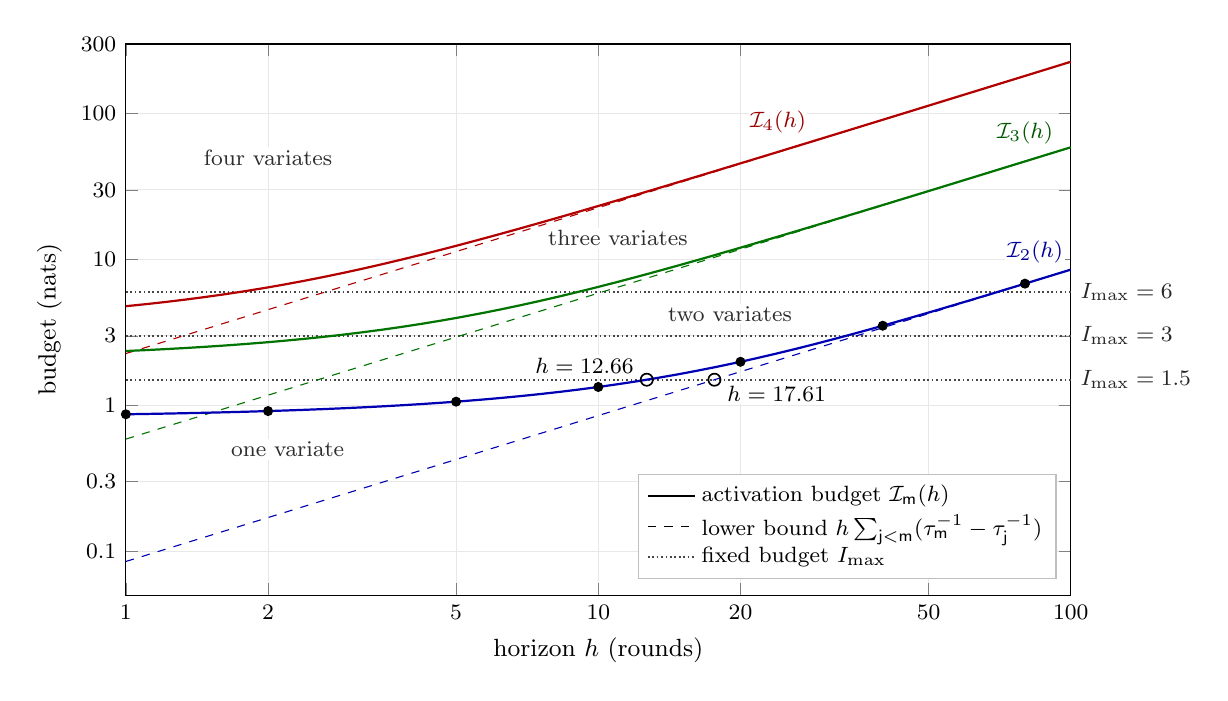
\begin{tikzpicture}
  \begin{axis}[width=12.0cm, height=7cm, scale only axis, xmode=log, ymode=log,
      xmin=1, xmax=100, ymin=0.05, ymax=300,
      xtick={1,2,5,10,20,50,100}, ytick={0.1,0.3,1,3,10,30,100,300}, log ticks with fixed point,
      grid=major, grid style={gray!18}, clip=false,
      xlabel={horizon $h$ (rounds)}, ylabel={budget (nats)},
      every axis label/.style={font=\small}, tick label style={font=\footnotesize},
      legend style={font=\footnotesize, at={(0.985,0.03)}, anchor=south east, draw=gray!50, fill=white,
        cells={anchor=west}, row sep=-1pt}]
    % fixed budgets
    \draw[gray!55!black, densely dotted, semithick] (axis cs:1,1.5) -- (axis cs:100,1.5);
    \draw[gray!55!black, densely dotted, semithick] (axis cs:1,3) -- (axis cs:100,3);
    \draw[gray!55!black, densely dotted, semithick] (axis cs:1,6) -- (axis cs:100,6);
    % linear lower bounds of prop:env-horizon(a), straight lines on these axes
    \addplot[blue!70!black, dashed, forget plot] coordinates {(1,0.085158) (100,8.5158)};
    \addplot[green!45!black, dashed, forget plot] coordinates {(1,0.58779) (100,58.779)};
    \addplot[red!70!black, dashed, forget plot] coordinates {(1,2.2666) (100,226.66)};
    % activation budgets I_2, I_3, I_4
    \addplot[blue!70!black, thick, forget plot] coordinates {(1,0.86926) (1.1007,0.87373) (1.2115,0.87868) (1.3335,0.88415) (1.4678,0.8902) (1.6156,0.8969) (1.7783,0.90432) (1.9573,0.91254) (2,0.9145) (2.1544,0.92165) (2.3714,0.93176) (2.6102,0.94298) (2.873,0.95545) (3.1623,0.96931) (3.4807,0.98474) (3.8312,1.0019) (4.217,1.0211) (4.6416,1.0425) (5,1.0607) (5.109,1.0663) (5.6234,1.0931) (6.1897,1.123) (6.8129,1.1565) (7.4989,1.1942) (8.254,1.2364) (9.0852,1.284) (10,1.3375) (11.007,1.3978) (12.115,1.4657) (13.335,1.5424) (14.678,1.6289) (16.156,1.7265) (17.783,1.8366) (19.573,1.9607) (20,1.9907) (21.544,2.1006) (23.714,2.2579) (26.102,2.4348) (28.73,2.6333) (31.623,2.8556) (34.807,3.1043) (38.312,3.382) (40,3.5169) (42.17,3.6914) (46.416,4.0358) (51.09,4.4185) (56.234,4.8432) (61.897,5.3138) (68.129,5.8347) (74.989,6.4107) (80,6.8328) (82.54,7.0471) (90.852,7.7496) (100,8.5247)};
    \addplot[green!45!black, thick, forget plot] coordinates {(1,2.3593) (1.1007,2.3931) (1.2115,2.4308) (1.3335,2.4729) (1.4678,2.5198) (1.6156,2.5723) (1.7783,2.631) (1.9573,2.6968) (2,2.7126) (2.1544,2.7705) (2.3714,2.8533) (2.6102,2.9463) (2.873,3.0509) (3.1623,3.1687) (3.4807,3.3014) (3.8312,3.451) (4.217,3.6197) (4.6416,3.81) (5,3.974) (5.109,4.0245) (5.6234,4.2662) (6.1897,4.5385) (6.8129,4.8449) (7.4989,5.1892) (8.254,5.5755) (9.0852,6.0084) (10,6.4926) (11.007,7.0333) (12.115,7.6361) (13.335,8.3071) (14.678,9.0529) (16.156,9.8808) (17.783,10.799) (19.573,11.815) (20,12.058) (21.544,12.94) (23.714,14.184) (26.102,15.558) (28.73,17.076) (31.623,18.751) (34.807,20.6) (38.312,22.639) (40,23.622) (42.17,24.887) (46.416,27.366) (51.09,30.098) (56.234,33.108) (61.897,36.425) (68.129,40.078) (74.989,44.103) (80,47.043) (82.54,48.534) (90.852,53.414) (100,58.788)};
    \addplot[red!70!black, thick, forget plot] coordinates {(1,4.7866) (1.1007,4.9402) (1.2115,5.113) (1.3335,5.3076) (1.4678,5.527) (1.6156,5.7742) (1.7783,6.053) (1.9573,6.3673) (2,6.4432) (2.1544,6.7215) (2.3714,7.1203) (2.6102,7.569) (2.873,8.0733) (3.1623,8.6392) (3.4807,9.2732) (3.8312,9.9825) (4.217,10.775) (4.6416,11.658) (5,12.411) (5.109,12.641) (5.6234,13.734) (6.1897,14.948) (6.8129,16.294) (7.4989,17.786) (8.254,19.437) (9.0852,21.263) (10,23.282) (11.007,25.513) (12.115,27.976) (13.335,30.695) (14.678,33.695) (16.156,37.004) (17.783,40.653) (19.573,44.676) (20,45.635) (21.544,49.11) (23.714,53.996) (26.102,59.379) (28.73,65.309) (31.623,71.841) (34.807,79.036) (38.312,86.959) (40,90.776) (42.17,95.684) (46.416,105.29) (51.09,115.87) (56.234,127.52) (61.897,140.34) (68.129,154.46) (74.989,170) (80,181.35) (82.54,187.11) (90.852,205.94) (100,226.67)};
    % values of chk:env-horizon(a) on I_2
    \addplot[only marks, mark=*, mark size=1.6pt, black, forget plot] coordinates {(1,0.8693) (2,0.9145) (5,1.0607) (10,1.3375) (20,1.9907) (40,3.5169) (80,6.8328)};
    % budget 1.5: I_2 reaches it at h = 12.664, the bound at the sufficient horizon 17.614
    \addplot[only marks, mark=o, mark size=2.2pt, black, semithick, forget plot] coordinates {(12.664,1.5) (17.614,1.5)};
    \node[font=\footnotesize, anchor=south east, inner sep=1pt, fill=white, xshift=-3.5pt, yshift=1pt] at (axis cs:12.664,1.5) {$h=12.66$};
    \node[font=\footnotesize, anchor=north west, inner sep=1pt, fill=white, xshift=3.5pt, yshift=-1pt] at (axis cs:17.614,1.5) {$h=17.61$};
    % curve labels
    \node[font=\footnotesize, blue!60!black, inner sep=0.5pt, fill=white] at (axis cs:84,11.2) {$\mathcal I_2(h)$};
    \node[font=\footnotesize, green!35!black, inner sep=0.5pt, fill=white] at (axis cs:80,74) {$\mathcal I_3(h)$};
    \node[font=\footnotesize, red!60!black, inner sep=0.5pt, fill=white] at (axis cs:24,88) {$\mathcal I_4(h)$};
    % regions: number of variates read at a budget in the region
    \node[font=\footnotesize, gray!35!black, inner sep=1pt, fill=white] at (axis cs:2.2,0.5) {one variate};
    \node[font=\footnotesize, gray!35!black, inner sep=1pt, fill=white] at (axis cs:19,4.24) {two variates};
    \node[font=\footnotesize, gray!35!black, inner sep=1pt, fill=white] at (axis cs:11,14) {three variates};
    \node[font=\footnotesize, gray!35!black, inner sep=1pt, fill=white] at (axis cs:2,50) {four variates};
    % budget labels outside the frame
    \node[font=\footnotesize, gray!30!black, anchor=west] at (axis cs:100,1.5) {$I_{\max}=1.5$};
    \node[font=\footnotesize, gray!30!black, anchor=west] at (axis cs:100,3) {$I_{\max}=3$};
    \node[font=\footnotesize, gray!30!black, anchor=west] at (axis cs:100,6) {$I_{\max}=6$};
    % legend of line styles
    \addlegendimage{black, thick}
    \addlegendentry{activation budget $\mathcal I_{\mathsf m}(h)$}
    \addlegendimage{black, dashed}
    \addlegendentry{lower bound $h\sum_{\mathsf j<\mathsf m}(\tau_{\mathsf m}^{-1}-\tau_{\mathsf j}^{-1})$}
    \addlegendimage{gray!55!black, densely dotted, semithick}
    \addlegendentry{fixed budget $I_{\max}$}
  \end{axis}
\end{tikzpicture}

  \caption{\textbf{Activation budgets rise with the horizon.} The budget $\mathcal I_{\mathsf m}(h)$ above which the $\mathsf m$-th canonical variate is read (\cref{thm:env-canonical}(b)), for $\mathsf m=2,3,4$ in the reversible exterior of \cref{chk:env-horizon}(a), with $\lambda(F)=(0.98,0.9,0.7,0.4)$, canonical correlations $\sigma_{\mathsf j}(h)=\lvert\lambda_{\mathsf j}(F)\rvert^h$ and $\kappa=4$ channels. The curves divide the plane into regions in which one to four variates are read. Each $\mathcal I_{\mathsf m}(h)$ is non-decreasing in $h$ and approaches its linear lower bound of \cref{prop:env-horizon}(a) (dashed) at long horizons, so the number of variates read at a fixed budget (dotted) falls as the horizon grows. With $I_{\max}=1.5$ nats two variates are read up to $h=12$ and one from $h=13$ on: $\mathcal I_2(h)$ reaches the budget at $h=12.66$, before the sufficient horizon $I_{\max}/(\tau_2^{-1}-\tau_1^{-1})=17.61$ at which its lower bound reaches it (circles). With $3$ nats the number falls from three to two and to one at $h=2.75$ and $33.48$, and with $6$ nats from four to three, two and one at $h=1.75$, $9.07$ and $70.10$. Dots mark the values of $\mathcal I_2(h)$ in \cref{chk:env-horizon}(a), from $0.869$ at $h=1$ to $6.833$ at $h=80$.}
  \label{fig:env-horizon}
\end{figure}

In a diffusive exterior on a connected graph the canonical variates at every horizon are the Laplacian eigenmodes in order of increasing Laplacian eigenvalue, so that the budget-optimal long-horizon sensor reads spatially coarse modes (Supplement, \cref{prop:env-diffusive}, under the hypotheses stated there).

\subsection{Control and expected free energy}\label{sec:env-control}

Information about the horizon is one reason to sense, and acting on preferred outcomes is another. We score sensors by an objective that contains both.

\begin{definition}[Horizon-$h$ attention objective]\label{def:env-attention-objective}
At round $t$ the agent chooses a sensor $s=H\eta_t+v$ and then an act $a=a(s)$, a measurable function of the reading. The act moves an outcome observed at $t+h$,
\[
o=H^{\mathrm o}\eta_{t+h}+B^{\mathrm o}a+v^{\mathrm o},\qquad v^{\mathrm o}\sim\Ncal(0,R^{\mathrm o}),
\]
with $B^{\mathrm o}$ of full column rank and $v^{\mathrm o}$ independent of everything else, and the agent prefers $\tilde p(o)=\Ncal(o^\ast,\Psi_{\mathrm o})$ with $\Psi_{\mathrm o}\succ0$. Its model target at the horizon is $\mathsf S_{\mathrm m}\eta_{t+h}$, with $\mathsf S_{\mathrm m}$ of full row rank ($\mathsf S_{\mathrm m}=I$ when the agent models the whole exterior). The horizon-$h$ attention objective is
\[
G^{\mathrm{att}}_h(H)=-I\bigl(s;\mathsf S_{\mathrm m}\eta_{t+h}\bigr)+\min_{a(\cdot)}\E\bigl[-\ln\tilde p(o)\bigr],
\]
minus the epistemic value about the model target at the horizon, minus the pragmatic value under the best contingent act. With $\mathbb P_{\mathrm o}=B^{\mathrm o}\bigl((B^{\mathrm o})^\top\Psi_{\mathrm o}^{-1}B^{\mathrm o}\bigr)^{-1}(B^{\mathrm o})^\top\Psi_{\mathrm o}^{-1}$, the control weight and its decision matrix are $\Upsilon_{\mathrm{ctl}}=(H^{\mathrm o})^\top\Psi_{\mathrm o}^{-1}\mathbb P_{\mathrm o}H^{\mathrm o}$ and $\mathsf J_{\mathrm{ctl}}=P_0^{1/2}(F^h)^\top\Upsilon_{\mathrm{ctl}}F^hP_0^{1/2}$.
\end{definition}
% src: H5-D2

A contingent act is what a recursive evaluation of expected free energy assumes, in which later acts are chosen given later beliefs \citep{friston2021sophisticated}, a work we know from its abstract. The epistemic term is a declared choice; \cref{rem:env-efe-horizon-free,rem:env-two-step} compute what the expected free energy of the framework, in the form of \cref{prop:fw-efe-communication}, gives instead.

\begin{theorem}[What a sensing-for-acting agent reads]\label{thm:env-control}
In the setting of \cref{def:env-attention-objective}, with $\mathsf X=\eta_t$:
\begin{enumerate}
\item[(a)] (Pragmatic term.) For every sensor and every measurable act rule, $\E[-\ln\tilde p(o)]\ge\mathfrak c_0+\frac12\tr(\Upsilon_{\mathrm{ctl}}\Cov(\eta_{t+h}\mid s))$, with a constant $\mathfrak c_0$ that does not depend on the sensor and equality for
\[
a^\ast(s)=-\bigl((B^{\mathrm o})^\top\Psi_{\mathrm o}^{-1}B^{\mathrm o}\bigr)^{-1}(B^{\mathrm o})^\top\Psi_{\mathrm o}^{-1}\bigl(H^{\mathrm o}\E[\eta_{t+h}\mid s]-o^\ast\bigr).
\]
Relative to no sensor the pragmatic value of $s$ is $\frac12\tr(\mathsf G_s\mathsf J_{\mathrm{ctl}})$. The weight $\Upsilon_{\mathrm{ctl}}\succeq0$ has rank at most $\rank B^{\mathrm o}$, and a reading has no pragmatic value exactly when it is uncorrelated with $\mathbb P_{\mathrm o}H^{\mathrm o}\eta_{t+h}$, the part of the preferred outcomes that acts can compensate.
\item[(b)] (Pure control.) Under rank $\kappa$ and budget $I_{\max}$ the sensor of largest pragmatic value reads leading eigenvectors of $\mathsf J_{\mathrm{ctl}}$ by reverse water-filling and uses at most $\rank B^{\mathrm o}$ channels, whatever $\kappa$ and $I_{\max}$.
\item[(c)] (Agreement.) Let $\mathsf C$ be the whitened cross-covariance of $(\eta_t,\mathsf S_{\mathrm m}\eta_{t+h})$. If $\mathsf C\mathsf C^\top$ and $\mathsf J_{\mathrm{ctl}}$ have a common orthonormal eigenbasis $(\mathsf e_{\mathsf j})$ along which both eigenvalue sequences, $\sigma_{\mathsf j}^2$ and $\lambda_{\mathsf j}(\mathsf J_{\mathrm{ctl}})$, are non-increasing, then every sensor satisfies
\[
G^{\mathrm{att}}_h(H)\ge\mathfrak c_0+\tfrac12\tr(\Upsilon_{\mathrm{ctl}}P_0)+\sum_{\mathsf j\le\kappa}\Bigl[\tfrac12\ln(1-\mathsf g_{\mathsf j}\sigma_{\mathsf j}^2)-\tfrac12\mathsf g_{\mathsf j}\lambda_{\mathsf j}(\mathsf J_{\mathrm{ctl}})\Bigr],
\]
with equality for the sensor that reads $\mathsf e_1,\dots,\mathsf e_\kappa$ in order. Under a rank limit and a budget, an optimal sensor for $G^{\mathrm{att}}_h$, one for predictive information alone and one for pragmatic value alone each read a leading segment $\mathsf e_1,\dots,\mathsf e_{\mathsf m}$ of this basis with capacities non-increasing along it; they can differ in $\mathsf m$ and in the allocation.
\item[(d)] Without a common co-monotone eigenbasis the selections can differ (\cref{ex:env-fast-preference}).
\end{enumerate}
\end{theorem}
% src: H5-T2

Proof in \cref{app:env}; checked in \cref{chk:env-control}.

The Supplement shows that, with world channels only and no preference, the expected free energy of the framework scores attention by information about the present state, which carries no horizon (\cref{rem:env-efe-horizon-free}), and that under a binding budget the epistemic term of its literal two-step form prefers the sensor least informative about the future outcome (\cref{rem:env-two-step}). In a two-mode instance of part (d) of \cref{thm:env-control}, at the larger of two preference weights on the fast mode the optimum of $G^{\mathrm{att}}_h$ reads the fast mode at $h=1,2$ and the slow mode from $h=3$ on (\cref{ex:env-fast-preference}).

\subsection{The selection principle and a cell}\label{sec:env-selection}

The nerve-cell example suggests three conditions for a variable to belong to an agent's environment: the blanket must couple to it, it must be predictable at the agent's horizon, and it must matter for the agent's preferences. \Cref{prop:env-selection} in the Supplement makes each a condition on the value of one added channel.

The channel has no value when it is uncorrelated with the exterior at the horizon given what the agent already reads, no pragmatic value exactly when it is uncorrelated, given those readings, with the part of the preferred outcomes that acts can compensate, and, for an independent Gauss--Markov content, a value bounded by terms that vanish geometrically in the horizon (Supplement, \cref{prop:env-selection}, under the hypotheses stated there); a variable whose innovation is small against the sensor noise yields little steady-state information per reading (Supplement, \cref{lem:env-constant}).

The Supplement applies the principle to a cell, with the noise of the chemical reading computed in \cref{prop:env-concentration}: in the model of \cref{ex:env-cell} one height reading of a buoyant protein has a signal-to-noise ratio more than thirteen orders of magnitude below one, against $0.79$ and $19.7$, in the leading term of the chemical noise, for one reading of a ligand signal of 1 and 5 percent of the mean concentration $\bar c_{\mathrm L}$, so that gravity fails the coupling clause, and it fails the relevance clause by construction of the model (\cref{rem:env-neurons} gives an interpretation). \Cref{fig:env-cell} draws the two ratios against the radius of the buoyant particle; in it $x_{\mathrm g}=\mathsf M_{\mathrm b}gZ_{\mathrm{box}}/(k_{\mathrm B}T_{\mathrm K})$ is the barometric exponent of a particle of buoyant mass $\mathsf M_{\mathrm b}$ in a compartment of height $Z_{\mathrm{box}}$, with $g$ the gravitational acceleration and $T_{\mathrm K}$ the absolute temperature.

\begin{figure}[!t]
  \centering
  % Figure: coupling of the chemical and gravitational channels of the cell of ex:env-cell (coupling clause,
% prop:env-selection(i)); signal-to-noise ratio of one reading against the radius of a buoyant particle.
% Chemoreception, ex:env-cell(1): the volume-time average of prop:env-concentration with r_cell = 5 um,
% D_m = 500 um^2/s, c_L = 1 nM = 0.6022 um^-3, T_int = 1 s, leading-term relative error
% (3/(5 pi D_m r_cell c_L T_int))^{1/2} = 1.1263e-2; a signal of 5 (1) percent of c_L has ratio
% (0.05/1.1263e-2)^2 = 19.707 ((0.01/1.1263e-2)^2 = 0.78829), as in ex:env-cell and chk:env-cell, which do not apply the
% finite-time factor 0.7897. It does not depend on the particle radius.
% Gravity sensing, ex:env-cell(4): ratio x_g^2/12 per independent reading, x_g = M_b g Z_box/(k_B T_K) with
% g = 9.81 m/s^2, Z_box = 10 um, T_K = 310 K, k_B = 1.380649e-23 J/K, and buoyant mass M_b = (4/3) pi r^3 Delta rho
% of a sphere with the density excess of protein, Delta rho = 369.86 kg/m^3 (partial specific volume 0.73 cm^3/g,
% water 1000 kg/m^3, buoyancy factor 0.27). The 50 kDa protein (1 Da = 1.66053907e-27 kg; M_b = 2.2417e-23 kg; a
% compact sphere of radius 2.4368 nm) has x_g = 5.1382e-7 and ratio 2.2000e-14, 13.658 orders of magnitude below one
% (arrow) and 13.554 below the 1-percent ligand signal, as in chk:env-cell. On these axes x_g^2/12 is a straight line
% of slope 6. x_g = 1 at r = 304.24 nm (shaded beyond, where sedimentation dominates; 275.15 nm at 500 kg/m^3). The
% Fisher ratio of one reading for eta^g = g is x_g^2 Var(z/Z_box) = 1 - (x_g/2)^2/sinh^2(x_g/2) for the truncated
% height law; x_g^2/12 is its small-x_g form, high by 0.13 percent at 166.4 nm and by 5.05 percent at x_g = 1 (1/12
% against 0.079326). The solid branch is x_g^2/12 up to 166.4 nm and ends on the exact value at x_g = 1. The dashed
% branch is the exact ratio with x_g = (r/304.24 nm)^3: it crosses 0.78829 at x_g = 4.642 (507.5 nm; 0.79 at 4.66,
% 508 nm), is 0.99447 at 650 nm and tends to one (x_g = 35.51 at 1 um, 284.08 at 2 um), so it never reaches 19.707.
% The form x_g^2/12 would reach 0.78829, 1 and 19.707 at x_g = 3.076, 3.464, 15.378 and is not the ratio of a reading
% there. The particle of radius 1 um with density excess 500 kg/m^3 has x_g = 48.005. The dashed coordinates were
% computed by work/fig_env_cell/exact_coords.py of the scratch area (mpmath, 30 digits, no random numbers; the closed
% form agrees with quadrature of the height law to 4e-31 for x_g < 60).
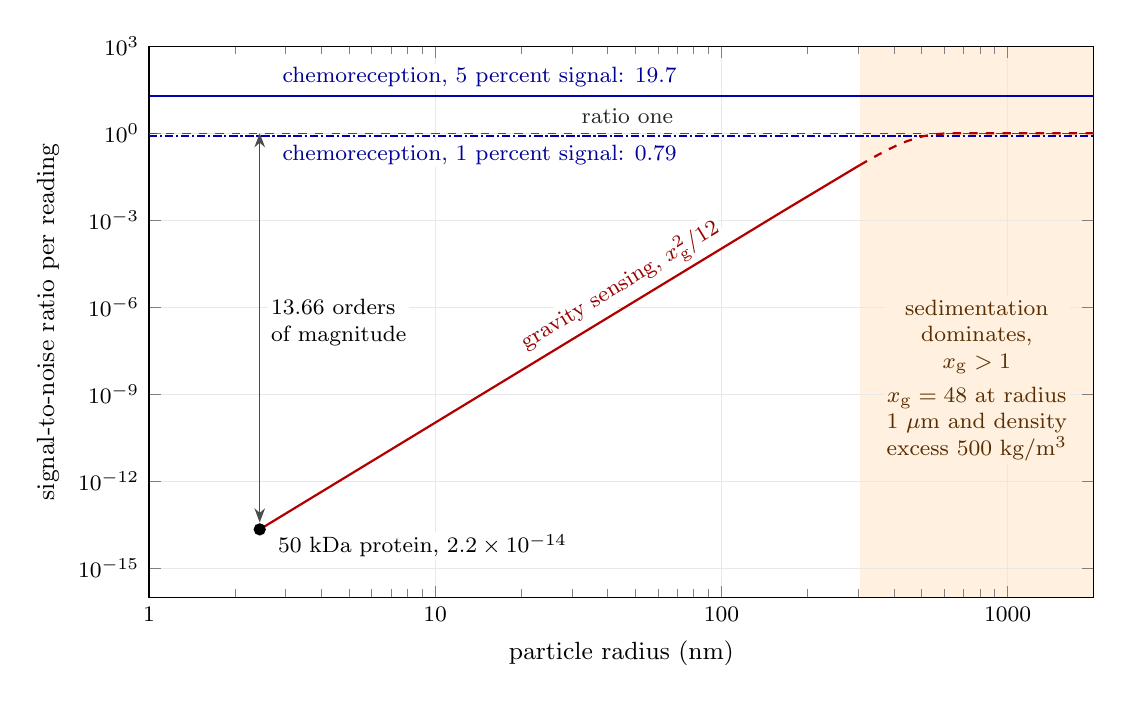
\begin{tikzpicture}[>={Stealth[length=1.8mm]}]
  \begin{axis}[width=12.0cm, height=7cm, scale only axis, set layers, xmode=log, ymode=log,
      xmin=1, xmax=2000, ymin=1e-16, ymax=1e3,
      xtick={1,10,100,1000}, xticklabels={$1$,$10$,$100$,$1000$},
      ytick={1e-15,1e-12,1e-9,1e-6,1e-3,1,1e3},
      grid=major, grid style={gray!18},
      xlabel={particle radius (nm)}, ylabel={signal-to-noise ratio per reading},
      every axis label/.style={font=\small}, tick label style={font=\footnotesize}]
    % regime where sedimentation dominates, x_g > 1 at the density of protein
    \begin{pgfonlayer}{axis background}
      \fill[orange!12] (axis cs:304.24,1e-16) rectangle (axis cs:2000,1e3);
    \end{pgfonlayer}
    \node[font=\footnotesize, orange!35!black, align=center, inner sep=1pt, fill=orange!12] at (axis cs:780,3e-9)
      {sedimentation\\dominates,\\$x_{\mathrm g}>1$\\[3pt]$x_{\mathrm g}=48$ at radius\\$1$ $\mu$m and density\\excess $500$ kg/m$^3$};
    % ratio one
    \draw[gray!60!black, dashed] (axis cs:1,1) -- (axis cs:2000,1);
    % chemoreception, ex:env-cell(1)
    \draw[blue!70!black, thick] (axis cs:1,19.707) -- (axis cs:2000,19.707);
    \draw[blue!70!black, thick, densely dashdotted] (axis cs:1,0.78829) -- (axis cs:2000,0.78829);
    % gravity sensing at the density of protein: x_g^2/12 solid for x_g <= 1, exact ratio dashed beyond
    \addplot[red!70!black, thick] coordinates {(2.4368,2.2e-14) (4.4552,8.2173e-13) (8.1455,3.0692e-11) (14.892,1.1464e-09) (27.228,4.2818e-08) (49.781,1.5993e-06) (91.016,5.9734e-05) (166.4,0.0022311) (304.24,0.079326)}
      node[pos=0.62, sloped, above=1pt, inner sep=1pt, fill=white, font=\footnotesize, text=red!60!black] {gravity sensing, $x_{\mathrm g}^2/12$};
    \addplot[red!70!black, thick, dashed] coordinates {(304.24,0.079326) (330,0.12533) (350,0.17268) (380,0.26431) (409.65,0.37751) (440,0.50913) (480,0.68384) (508,0.78989) (551.58,0.90782) (600,0.97253) (650,0.99447) (742.68,0.9999) (1000,1) (2000,1)};
    % the 50 kDa protein
    \addplot[only marks, mark=*, mark size=2.0pt, black] coordinates {(2.4368,2.2e-14)};
    \node[font=\footnotesize, anchor=west, inner sep=1pt, fill=white] at (axis cs:2.75,6e-15) {$50$ kDa protein, $2.2\times10^{-14}$};
    % gap to a ratio of one
    \draw[<->, black!70, shorten <=2.5pt] (axis cs:2.4368,2.2e-14) -- (axis cs:2.4368,1);
    \node[font=\footnotesize, anchor=west, align=left, inner sep=1pt, fill=white] at (axis cs:2.6,3e-7) {$13.66$ orders\\of magnitude};
    % labels of the lines
    \node[font=\footnotesize, blue!60!black, anchor=south west, inner sep=1pt, fill=white, yshift=2pt] at (axis cs:2.85,19.707) {chemoreception, $5$ percent signal: $19.7$};
    \node[font=\footnotesize, blue!60!black, anchor=north west, inner sep=1pt, fill=white, yshift=-2pt] at (axis cs:2.85,0.78829) {chemoreception, $1$ percent signal: $0.79$};
    \node[font=\footnotesize, gray!30!black, anchor=south west] at (axis cs:30,1) {ratio one};
  \end{axis}
\end{tikzpicture}

  \caption{\textbf{The coupling clause for a cell.} Signal-to-noise ratio of one reading, the coupling of items (1) and (4) of \cref{ex:env-cell}. Chemoreception (blue), the volume-time average of \cref{prop:env-concentration} over $T_{\mathrm{int}}=1$~s with relative error $1.13\times10^{-2}$ (leading term), has ratio $19.7$ for a ligand signal of 5 percent of $\bar c_{\mathrm L}$ and $0.79$ for 1 percent, independent of the particle radius. Gravity sensing by the equilibrium height of a buoyant particle in a compartment of height $Z_{\mathrm{box}}=10$~$\mu$m has ratio about $x_{\mathrm g}^2/12$ for $x_{\mathrm g}\ll1$ (red), which grows as the sixth power of the radius; it is drawn for particles with the density of protein (buoyancy factor $0.27$, density excess $370$~kg/m$^3$). A $50$~kDa protein, a sphere of radius $2.44$~nm at partial specific volume $0.73$~cm$^3$/g, has $x_{\mathrm g}=5.1\times10^{-7}$ and ratio $2.2\times10^{-14}$, $13.66$ orders of magnitude below a ratio of one (gray dashed) and $13.55$ below the 1 percent ligand signal; this compares one height sample of one protein with a chemical reading that pools about $10^4$ molecule-samples, and at equal pooling the gravity ratio is $2\times10^{-10}$. Below $x_{\mathrm g}=1$, reached at radius $304$~nm, the ratio stays under $1/12$, below both ligand signals. Beyond it (shaded) the scale height $k_{\mathrm B}T_{\mathrm K}/(\mathsf M_{\mathrm b}g)=Z_{\mathrm{box}}/x_{\mathrm g}$ is shorter than the compartment and sedimentation dominates thermal motion; the exact ratio $1-(x_{\mathrm g}/2)^2/\sinh^2(x_{\mathrm g}/2)$ is drawn dashed there: it is $0.079$ at $x_{\mathrm g}=1$, passes the 1 percent ligand ratio $0.79$ at $x_{\mathrm g}=4.66$ (radius $508$~nm) and approaches one from below, so that no particle in this model reaches the 5 percent ligand ratio per reading. A particle of radius $1$~$\mu$m and density excess $500$~kg/m$^3$ has $x_{\mathrm g}=48$.}
  \label{fig:env-cell}
\end{figure}

\subsection{Aggregates as an abstract environment}\label{sec:env-aggregates}

Many sensors read aggregates of many agents: a price, an index, a poll, an average. \Cref{thm:met-abstract-physics} gives the criterion for a declared coarse exterior to have an exact abstract physics, and \cref{def:met-lumpable} its form for block sums; here we ask when aggregates of many agents meet it and how much memory they carry when they do not.

An outside agent whose channels read only aggregates, with noise, has them among its external states: physical in being functions of the joint process, abstract in not being the base-level world.

In the Supplement, with the vocabulary of \cref{def:env-aggregates}, the average of a linear recursion is exactly closed if and only if all column sums of the update matrix are equal, and the type averages of interchangeable types are exactly closed together with the world (\cref{prop:env-aggregate-closure}); for uncoupled autoregressive members the average is Markov if and only if all persistences are equal, its Markov error is bounded through their dispersion, and a continuum of persistences that reaches the unit root gives long memory (\cref{prop:env-aggregate-memory}, each part under the hypotheses stated there).

\subsection{The Hayek dimension at a horizon, firms and people}\label{sec:env-hayek}

\Cref{prop:abs-hayek} counts the public scalars that make private decisions exact. With dynamics, a decision about the future depends on the present through $(F^h)^\top\psi_i$, and the count depends on the horizon.

\begin{theorem}[The Hayek dimension at a horizon]\label{thm:env-hayek-horizon}
Let agent $i$'s decision be evaluated against $\psi_i^\top\eta_{t+h}$ with quadratic loss, let it sense $s_i=H^s_i\eta_t+v_i$ with $R^s_i\succ0$, and let a public message $M\eta_t$ be available.
\begin{enumerate}
\item[(a)] (Exact sufficiency.) The full-information loss $\Var(\psi_i^\top\eta_{t+h}\mid\eta_t)$ is attained given $(s_i,M\eta_t)$ if and only if $(F^h)^\top\psi_i\in\operatorname{row}(M)$. The public message suffices for every agent if and only if $(F^h)^\top\operatorname{span}\{\psi_i\}\subseteq\operatorname{row}(M)$, and the least number of public scalars that suffices is $r_{\mathrm{Hay}}(h)=\dim(F^h)^\top\operatorname{span}\{\psi_i\}$, non-increasing in $h$ and constant when $F$ is invertible.
\item[(b)] (Effective dimension, reversible exteriors.) For a common horizon, the total excess loss of a noiseless public message of rank $r_M$, ignoring private signals, which bounds each agent's excess above, is at least $\sum_{\mathsf j>r_M}\lambda_{\mathsf j}(\mathsf D_h)$ with $\mathsf D_h=P_0^{1/2}(F^h)^\top(\sum_i\psi_i\psi_i^\top)F^hP_0^{1/2}$, and the leading eigenvectors of $\mathsf D_h$ attain it. Let $FP_0=P_0F^\top$, with $\mathsf e_{\mathsf j}$ the orthonormal eigenvectors of $\mathsf F$ ordered by decreasing $\lvert\lambda_{\mathsf j}(F)\rvert$ and decision weights $\mathsf w_{\mathsf j}=\sum_i(\mathsf e_{\mathsf j}^\top P_0^{1/2}\psi_i)^2$, and let $h\ge1$, $\lambda_1(F)\ne0$ and $\mathsf w_1>0$. The message that reads the $r_M$ slowest mode amplitudes has relative excess loss, its share of $\tr\mathsf D_h$,
\[
\frac{\sum_{\mathsf j>r_M}\lvert\lambda_{\mathsf j}(F)\rvert^{2h}\mathsf w_{\mathsf j}}{\sum_{\mathsf j}\lvert\lambda_{\mathsf j}(F)\rvert^{2h}\mathsf w_{\mathsf j}}\le\Bigl(\frac{\lvert\lambda_{r_M+1}(F)\rvert}{\lvert\lambda_1(F)\rvert}\Bigr)^{2h}\frac{\sum_{\mathsf j>r_M}\mathsf w_{\mathsf j}}{\mathsf w_1},
\]
and the effective Hayek dimension at tolerance $\mathfrak e$, the least rank with relative excess at most $\mathfrak e$, is at most $\#\{\mathsf j:\lvert\lambda_{\mathsf j}(F)\rvert\ge\lvert\lambda_1(F)\rvert(\mathfrak e\mathsf w_1/\sum_{\mathsf j'}\mathsf w_{\mathsf j'})^{1/(2h)}\}$, which tends to the number of modes of largest modulus as $h\to\infty$.
\item[(c)] (Diagonalizable exteriors.) With right and left eigenvectors $\mathsf r_{\mathsf j}$ and $\mathsf u_{\mathsf j}$ of $F$, normalized so that $\mathsf u_{\mathsf j}^\top\mathsf r_{\mathsf j}=1$ and $\mathsf u_{\mathsf j}^\top\mathsf r_{\mathsf j'}=0$ for $\mathsf j'\ne\mathsf j$, and $\lvert\lambda_{r_M}(F)\rvert>\lvert\lambda_{r_M+1}(F)\rvert$, a message that reads the real span of the slowest $r_M$ mode amplitudes leaves, for a decision $\psi^\top\eta_{t+h}$, an excess loss at most $\bigl(\sum_{\mathsf j>r_M}\lvert\lambda_{\mathsf j}(F)\rvert^h\lvert\psi^\top\mathsf r_{\mathsf j}\rvert(\mathsf u_{\mathsf j}^*P_0\mathsf u_{\mathsf j})^{1/2}\bigr)^2$, which is $O(\lvert\lambda_{r_M+1}(F)\rvert^{2h})$, while the decision variance $\Var(\psi^\top F^h\eta_t)$ is of order $\lambda_1(F)^{2h}$ when $\lambda_1(F)$ is real, simple and of strictly largest modulus and $\psi^\top\mathsf r_1\ne0$.
\end{enumerate}
\end{theorem}
% src: H5-T3

Proof in \cref{app:env}; checked in \cref{chk:env-hayek}. The exact Hayek dimension does not shrink with the horizon for invertible dynamics, but the effective one does: long-horizon decisions need only the amplitudes of the slowest modes, and a public signal of their rank suffices up to an error that decays geometrically in the horizon. In a reversible exterior with six modes and ten random decisions the effective dimension at tolerance $0.05$ falls from 4 at $h=0$ to 1 from $h=50$ on. Rational inattention models agents whose actions depend on observations through a channel of finite Shannon capacity \citep{sims2003implications}, which we know from its record and a secondary account; in a model of price setting under rational inattention, firms attend more to firm-specific than to aggregate conditions when the former are more volatile or more consequential \citep{mackowiak2009optimal}, which we know from its abstract. Two examples in the Supplement (\cref{ex:env-firm,ex:env-person}) are linear-Gaussian instances of such selection.

A firm with a production lag in a two-mode market finds the futures price of its own lag sufficient, a known separation result recovered, and, with the price noise neglected and the price taken as exogenous, the spot price better than a slow index exactly below an explicit crossover horizon (Supplement, \cref{ex:env-firm}, read as a meta-agent in \cref{rem:env-firm-meta-agent}); a person with three decisions at horizons 1, 8 and 40 in a four-mode economy reads, under a Shannon budget, one slow aggregate at small budgets and a second channel only above $0.72$ nats per period (Supplement, \cref{ex:env-person}).

Two further results are in the Supplement (\cref{sec:env-levels}). Along a jointly Gaussian Markov chain the whitened cross-covariances multiply, which bounds what passes from the world through an aggregate to its reader (\cref{lem:env-composition}). For a person who reads the physical world and the aggregates of its memberships, the information that the physical channel adds to the aggregates about a scalar decision obeys a bound that decays geometrically in the horizon, and a Shannon budget couples the attention to different memberships only through a common water level (\cref{prop:env-multiplex}, each part under the hypotheses stated there). \Cref{rem:env-own-aggregate} treats a reader whose own report enters the aggregate, and \cref{rem:env-interpretation} interprets the results of this section for corporations, people and cells.

Left open in the Supplement (\cref{sec:env-open}) are the optimal sensor of an agent that integrates its readings with a Kalman filter (\cref{open:env-filtering}) and the conjecture that, beyond linear-Gaussian exteriors, the optimal predictive representations concentrate at long horizons on functions invariant under the slowest part of the dynamics (\cref{conj:env-nonlinear}).

% 10e_open_problems.tex: assembled from a head (introduction and table) and ten parts, one per problem.
\section{Open problems posed in the literature}\label{sec:opn}

This section sets the manuscript against ten open problems drawn from the recent literature on collective active inference. For each problem a subsection states the question as the literature poses it, reports what the manuscript establishes, and names what remains open. In each account the results of the main text come first, together with those of its statements that are placed in the supplement; they are followed by the extensions, which are developed in the supplement together with their proofs and numerical checks. Every statement holds in the model in which it is proved, and no problem is closed in the generality in which it was posed. Two problems are addressed only by a scoped model. For energetic viability (\cref{sec:opn-8}), the conversion of information into energy rests on three premises that are declared and not derived, and it yields necessary conditions only. For evolutionary individuality (\cref{sec:opn-9}), reproduction is imposed as a fission and fitness is supplied as an input. \Cref{tab:opn-status,tab:opn-status-b} list, for each problem, what is established, where, and what stays open.

\begin{table}[p]
\centering
\small
\caption{The open problems of \cref{sec:opn-1,sec:opn-2,sec:opn-3,sec:opn-4,sec:opn-5}: what the manuscript establishes, where, and what remains open. Numbers with the prefix S refer to the supplement. The table continues in \cref{tab:opn-status-b}.}
\label{tab:opn-status}
\begin{tabular}{@{}>{\raggedright\arraybackslash}p{0.13\textwidth}>{\raggedright\arraybackslash}p{0.33\textwidth}>{\raggedright\arraybackslash}p{0.17\textwidth}>{\raggedright\arraybackslash}p{0.29\textwidth}@{}}
\toprule
Problem & Established & Where & Open \\
\midrule
Collective agency & Exact path-blanket criterion; blanket existence selects nothing; exact conditional meta-agent theorem; relative-entropy error terms under declared closure defects; recorded predictability and persistence cannot grade agency, invariant channel interventions certify interaction. & \cref{thm:col-path-blanket,thm:met-h5a}; Supplement, \cref{cor:apx-uniform,thm:idn-intervention} & Approximate meta-agent theorem with persistence, with a bounded memory of the coarse internal state, or beyond stable linear-Gaussian collectives; estimator of interaction without a recorded shared drive; observed population meeting all requirements. \\
\addlinespace
Controlled renormalization & Exact reductions with memory kernels and closure conditions; for stable linear-Gaussian collectives, a uniform path relative-entropy bound over small-gain policies, geometric bound in filter order, score and level bounds; for stable linear diffusions with invertible noise factors, the first-order error of the memoryless elimination of fast internal states. & \cref{thm:ren-memory,thm:met-abstract-physics}; Supplement, \cref{cor:apx-uniform,thm:apx-order-d,prop:ren-adiabatic-rate} & Nonlinear or non-Gaussian dynamics, policies without small gain, continuous time; sharp posterior bound; the items of \cref{open:ren-beyond} of the supplement. \\
\addlinespace
Recursive formation & Inherited law of a formed group, exact at the idealized split; level-two thresholds and obstructions for the frozen-calibration mean-field map; lower bounds growing with depth; no nested meta-agent established. & \cref{thm:frm-formation}; Supplement, \cref{prop:rfm-inheritance,thm:rfm-thresholds,prop:rfm-verdict} & Stochastic model with tracking calibration; full exact-fusion null at level two; a level-two model with acts; frame classes and aggregate channel still supplied. \\
\addlinespace
Conflicting objectives and collective policy & Under a declared protocol, reversibility, exact potential game and agreement on redundancy are equivalent; for quadratic preferences, conditional closed forms for rotation, cost and deliberation time, and tests identifying conflict. & \cref{thm:agy-agency}; Supplement, \cref{thm:obj-rotation,prop:obj-cost,prop:obj-identification} & Nonsymmetric heat-bath laws beyond two scalar members, preferences that are not quadratic, simultaneous moves, mutual learning, institutions with undeclared protocol. \\
\addlinespace
Evidence provenance and institutional memory & One shared linear-Gaussian state: exact link storage on process-noise-free trees and full-rate stars; with nondegenerate process noise and an invertible transition matrix, intermittent blind reports need ledgers; no anonymous exact protocol on two cycle sizes; static turnover loss. & \cref{thm:hie-messages}; Supplement, \cref{thm:prv-tree,thm:prv-window,prop:prv-turnover} & Dynamic hierarchies with distinct node variables; least storage on graphs with cycles; uncertain source overlap; closed-form turnover loss under process noise. \\
\bottomrule
\end{tabular}
\end{table}

\begin{table}[p]
\centering
\small
\caption{The open problems of \cref{sec:opn-6,sec:opn-7,sec:opn-8,sec:opn-9,sec:opn-10}, continuing \cref{tab:opn-status}.}
\label{tab:opn-status-b}
\begin{tabular}{@{}>{\raggedright\arraybackslash}p{0.13\textwidth}>{\raggedright\arraybackslash}p{0.33\textwidth}>{\raggedright\arraybackslash}p{0.17\textwidth}>{\raggedright\arraybackslash}p{0.29\textwidth}@{}}
\toprule
Problem & Established & Where & Open \\
\midrule
Learned interfaces and shared meaning & Linear-Gaussian: grounded pairs identify codes on attended directions; ungrounded, up to orthogonal groups under known symmetric dynamics; drift floor of order $q^{1/2}$; four-term risk; hub codes transfer to unmet partners. & \cref{prop:fw-grounded-identification}; Supplement, \cref{thm:lrn-gauge,thm:lrn-risk-decomposition,thm:lrn-path} & Choice of interface for a task; joint learning of code, dynamics and state; strategic senders; nonlinear representations. \\
\addlinespace
Scale and time laws & A predictive-information criterion selects ranks in spectral gaps, in the nested medium the levels; for $\mathfrak{q}<1$ at large depth, relaxation time grows as a power of block size until saturation. & \cref{thm:ren-nested}; Supplement, \cref{thm:obj-selection,thm:obj-nested,prop:obj-clocks} & Endogenous choice of the medium, frames that are not invariant, nonreversible drifts, the regions the Laplacian procedure returns; no universality class. \\
\addlinespace
Energetic viability & Closed-form entropy production of the stationary even linear-Gaussian joint process; coarse linear descriptions hide dissipation; under three declared premises, necessary size conditions for memoryless agents. & Supplement, \cref{thm:nrg-ep,thm:nrg-coarse,thm:nrg-flow,thm:nrg-scale} & Derivation of the bridge premises; any sufficient condition for viability; the rate retained by a coarse description; agents with memory. \\
\addlinespace
Evolutionary individuality & In a declared fission model with fitness as an input, the heritability of a convention as a spectral radius below one; a copied record sustains it without founders. & \cref{prop:agy-identity}; Supplement, \cref{prop:evo-transmission,thm:evo-record-channel,prop:evo-price} & Fitness and reproduction derived from the dynamics; heritable organizational parameters; tradeoffs between collective traits. \\
\addlinespace
Empirical identification & In the linear-Gaussian model the stationary covariance identifies nothing about interaction, the path law separates pure interaction from low-rank regular drivers only, and invariant channel interventions can certify it. & \cref{prop:agy-tests}; Supplement, \cref{thm:idn-path,thm:idn-intervention,prop:idn-grade} & Interaction and a colored low-rank driver together, sharp bounds, finite-sample tests, a test of the invariance hypotheses, an identification study on a real system. \\
\bottomrule
\end{tabular}
\end{table}

\subsection{Collective agency}\label{sec:opn-1}

The first problem asks when a collection warrants a model as an agent, with a defensible internal state, external variables it predicts, actions it controls, and persistence over a stated horizon. The nested-blanket program \citep{kirchhoff2018markov} motivates the question; a statistical blanket alone does not answer it. The foundational dispute \citep{biehl2021technical,aguilera2022particular,heins2022sparse} shows one must say which independence is meant, and positive results hold under stated hypotheses \citep{dacosta2021bayesian,friston2023path}. A workable form accounts for hidden common drivers and grades agency by prediction error, control error and persistence time.

In the linear-Gaussian framework the main text separates instantaneous blankets, path blankets and leak rates (\cref{def:col-blankets}) and proves an exact criterion for a finite-window path blanket (\cref{thm:col-path-blanket}). Blanket existence selects nothing: with separate channels and per-channel noise every set of agents is an exact path blanket (Supplement, \cref{prop:col-selects-nothing}). Selection rests on contrast above a declared level and a homogeneous baseline (\cref{def:col-collective}), and a meta-agent is graded by closure tolerances, nulls and an agency index (\cref{def:agy-meta-agent}). Under explicit hypotheses a set of agents has an exact coarse blanket, a closed internal state, a predictive law of its exterior and a group policy posterior (\cref{thm:met-h5a}); it is exact and conditional, and holds even when members exchange no contributions (\cref{rem:met-no-selection}). When closure fails by a declared amount the supplement proves, for stable linear-Gaussian collectives, a uniform bound over small-gain coarse policies on the relative entropy between the retained controlled path law and a declared Markov model (\cref{cor:apx-uniform}), and a bound on the stationary excess relative entropy of a meta-agent filtering with that model, which needs no smallness condition (\cref{thm:apx-unconditional}); with the exact blanket and the exact closure of the internal state these give an approximate form of \cref{thm:met-h5a} for collectives whose members run the consensus filter (\cref{thm:apx-h5a}). When the blanket conditions fail as well, the closure of the internal state stays exact and the error terms hold with the members' channels as the record, an observation defect added to the closure defect, and the belief measured in the stationary limit against the law of the exterior given those channels (Supplement, \cref{thm:apx-h5a-blanket}). For an unrecorded common driver the supplement's results are mostly negative: the stationary covariance identifies nothing about interaction (\cref{thm:idn-covariance}), and an interaction-free model attains any prescribed predictability below one and persistence time on records (\cref{prop:idn-grade}). A channel intervention on cross gains alone that leaves the driver law and loading unchanged certifies interaction whenever it changes the recorded law (Supplement, \cref{thm:idn-intervention}).

An approximate form of \cref{thm:met-h5a} outside the stable linear-Gaussian setting treated, the sharp constant of its error term in terms of the closure defect, a bound in terms of the defects on the leak of the coarse blanket when the blanket conditions are violated, and the memory of the coarse internal state under level-0 protocols beyond scalar members with exact code models, and for such members the Markov error of their average when the exterior responds, are open (Supplement, \cref{open:met-approximate,open:apx-sharp,open:apx-beyond,open:apx-internal}), and the bounds obtained omit persistence. An estimator of interaction without a recorded shared drive remains open, as do identifiability under interaction with a colored low-rank driver, finite-sample tests, and a test of the assumed invariance (Supplement, \cref{open:agy-unrecorded-drive,open:idn-mixed,open:idn-sharp,open:idn-invariance}). No observed population is shown to meet the combined requirements.

\subsection{Controlled renormalization}\label{sec:opn-2}

The second problem asks what coarse-graining preserves of predictions and of controlled responses, and with what error. Eliminating variables generally introduces memory, correlated fluctuations and new interactions, and matching a stationary density is a weaker target than matching responses to new policies. The constructions that group variables and retain slow modes \citep{friston2019free,friston2021parcels} are conditional and, in the parts we read, leave open how errors accumulate at finite timescale separation; this reading does not cover the engineering perspective on active inference of \citet{devries2026active}, which we have not read. The target is a bound, uniform over a declared policy class for a declared lifting and horizon, between the coarse-grained controlled law and a coarse model; information-theoretic renormalization, known to us from the record of \citet{lenggenhager2020optimal} and the abstract of \citet{gordon2021relevance}, gives conditional results not yet extended to controlled adaptive processes.

The main text distinguishes exact marginalization, exact pushforward and Galerkin projection (\cref{def:ren-maps}). For a stationary reversible linear-Gaussian population the exact reduction carries a memory kernel whose time integral is the static correction to the projected precision (\cref{thm:ren-memory}); the law of block averages is in general not diffusive, and the coarse level-0 network has a memory term that vanishes exactly for lumpable partitions (\cref{thm:ren-closure}). A coarse exterior driven by a coarse act is exactly Markov precisely when an algebraic closure condition holds (\cref{thm:met-abstract-physics}). In discrete time the supplement proves a statement of the requested form for stable linear-Gaussian collectives and causal small-gain coarse policies: the relative entropy between the retained controlled path law and a declared Markov coarse model obeys an exact identity and a bound uniform over the policy class and linear in the horizon (Supplement, \cref{thm:apx-path,cor:apx-uniform}). In a two-variable example with a colored orthogonal force, truncating the memory kernel at any order and whitening that force leaves a positive relative-entropy rate (Supplement, \cref{prop:apx-kernel-floor}), whereas truncating the filter of the unresolved coordinate at order $d$ gives a one-step error bounded by a term decaying geometrically in $d$ from round $d+1$ on (Supplement, \cref{thm:apx-order-d}). For a quadratic score, the errors of the score and of the policy posterior are bounded through the same defect (Supplement, \cref{prop:apx-score,prop:apx-softmax}), and defects compose through levels (Supplement, \cref{thm:apx-levels}).

These results settle none of the items of \cref{open:ren-beyond} of the supplement. Of those items, nonreversible discrete-time closure is treated for one coordinate only, where the Markov error of a stable recursion with the exterior held fixed is bounded under a power bound on the deviation block (Supplement, \cref{thm:apx-markov-discrete}) and the joint form for several blocks stays open. Separately from these results, a former item of that list is settled under hypotheses: for a stable linear diffusion with invertible noise factors whose internal states and internal noise intensity are sped up by a common factor, with the internal drift and the quasi-static drift stable, the error of the memoryless reduction is, to leading order and uniformly over lags, a proved coefficient times the inverse of that factor (Supplement, \cref{prop:ren-adiabatic-rate}). Nonlinear or non-Gaussian dynamics, policies without small gain and the continuous-time limit are open (Supplement, \cref{open:apx-beyond}), as is a sharp bound on the belief of a coarse filter (Supplement, \cref{open:apx-sharp}). In this setting the epistemic part of the score does not depend on the policy (Supplement, \cref{lem:apx-separation}), so information-seeking action is not tested.

\subsection{Recursive formation}\label{sec:opn-3}

A hierarchy can be supplied by its designer, learned as a state abstraction, or formed by its interacting constituents. The open question concerns the third: when local sensing, communication, action and resource limits produce a new predictive unit, and then a further level from the dynamics the first actually inherited. \citet{palacios2020markov} simulate assembly under role-related priors and illustrate a second organizational level; the demonstration is constructive, with supplied ingredients, since its higher level represents one ensemble explicitly and the others in mean field and defines coarse sensing and action by averaging. An answer would fix its collective criterion beforehand and be tested under improved evidence fusion.

In the linear-Gaussian two-group model of \cref{def:frm-two-group}, with frame classes given in advance, \cref{thm:frm-formation} proves thresholds for the frozen-calibration mean-field map, and \cref{thm:frm-split-contrast} proves that at infinite policy precision, with $\kappa\le n-1$ senders attended by each receiver in groups of $n$ members, exact in-group translations and nonzero cross translation errors, the two groups are exactly the collectives at the levels of a stated window. \Cref{prop:frm-exact-fusion} proves that receivers who know their translation errors select no split from start laws exchangeable given the world path. \Cref{thm:ren-nested,thm:hie-three-levels} concern hierarchies whose nesting is supplied. At the idealized first split a formed group hands on its exterior noise, memory, error covariance, frame and outgoing calibration, the aggregate channel being an added hypothesis (Supplement, \cref{prop:rfm-inheritance}). For the frozen-calibration mean-field map, level-two thresholds and conditions that block the second event are proved, with lower bounds on the thresholds that grow with depth (Supplement, \cref{thm:rfm-thresholds,thm:rfm-obstruction,cor:rfm-depth}). The outcome is negative in part. As a numerical observation at the base point, the contrast of a parent falls from $8.73$ to $1.33$ when its superunit forms: the second event replaces the first level and does not nest it at a common grade (Supplement, \cref{obs:rfm-window}). The model has no acts, and with a translation-aware null admitted among the nulls of type S and evaluated at its symmetric stationary laws the superunit is not a meta-agent at any grade (Supplement, \cref{prop:rfm-null,prop:rfm-verdict}). No nested meta-agent is established.

Recursive formation is not established. The inherited law is established only at the idealized split, frame classes are given in advance at both levels, and whether the stochastic model with calibration that tracks the forming law reaches either split is open (\cref{open:frm-closure}; Supplement, \cref{open:rfm-online}). Open as well are the second event under full exact fusion, a level-two model with acts, competition among parents for capacity, and closure under turnover (Supplement, \cref{open:rfm-exact-fusion,open:rfm-agent,open:rfm-competing,open:rfm-turnover}). Formation that survives exact fusion remains a conjecture (Supplement, \cref{conj:hie-conformity-formation}).

\subsection{Conflicting objectives and collective policy}\label{sec:opn-4}

Organizations contain parts with competing demands, and agreement about facts need not coincide with agreement about preferred outcomes. The open problem is to determine when such constituents admit a collective generative model or policy law derived from their own update and decision rules, and when a game-theoretic or multi-objective description must be retained. The voting example of \citet{waade2025one} fixes the blanket architecture, omits learning and fits an action precision whose confounding with preferences its authors recognize; in the strategic setting of \citet{ruizserra2025factorised} the aggregate expected free energy need not decrease; the spin-glass correspondence of \citet{heins2023spin} assumes symmetric precision and a stated update rule.

Under a declared protocol in which members share data and intentions and resample their policies one at a time from their own expected free energies, (P1) to (P4) of \cref{def:agy-group-model}, \cref{thm:agy-agency} proves that deliberation is reversible if and only if the expected free energies form an exact potential game, if and only if every two members agree on the conditional redundancy of their inputs; the stationary law is then a group posterior with tilted habits whenever a declared belief has the agreed redundancies. Without that agreement \cref{thm:agy-heterogeneous} bounds its distance from the Gibbs law of a potential. For quadratic preferences over additive acts the supplement proves that deliberation on every finite act set is reversible exactly when the antisymmetric part of the interaction matrix vanishes (Supplement, \cref{thm:obj-rotation}), with closed forms for the cost of disagreement about targets under shared precision and effect models (Supplement, \cref{prop:obj-cost}) and for the spectral gap of heat-bath deliberation under symmetric positive definite interaction (Supplement, \cref{thm:obj-time}). Two results are negative: for two members with scalar acts an exact potential game can have no stationary law under either protocol (Supplement, \cref{prop:obj-protocol}), and under Langevin deliberation a stationary cross-section of acts never identifies conflict, which shows instead in an asymmetric mean response to shifted loads or in time-irreversible lagged covariances (Supplement, \cref{prop:obj-identification}).

These statements assume a declared protocol, and those of the extension quadratic preferences over additive acts. The heat-bath stationary law for nonsymmetric interaction beyond two scalar members, preferences that are not quadratic, interacting effects, simultaneous moves and members who learn about one another are open (Supplement, \cref{open:obj-strategic}); simultaneous revision by three or more members is covered only by a conjecture (Supplement, \cref{conj:agy-synchronous}). Whether an actual institution meets the protocol hypotheses is open as well (Supplement, \cref{open:abs-institutions}), as is agency for policies whose acts change what observations reveal (Supplement, \cref{open:agy-mixed-policies}).

\subsection{Evidence provenance and institutional memory}\label{sec:opn-5}

A collective often receives a summary built partly from its own earlier signals, and a member that treats it as independent gains confidence without evidence. The problem is to keep collective memory calibrated under repeated communication, uncertain source overlap, changing membership and imperfect interpretation. \citet{nomura2026social} model the reciprocal development of social priors and environmental structure, \citet{march1991exploration} models mutual learning between individuals and an organizational code, and \citet{sasaki2017cumulative} report improved pigeon navigation across successive replacement of members. The first leaves open calibrated accounting of evidence for records with overlapping origins; the others concern organizational learning and task-specific transmission.

In the Gaussian tree model, exact inference sends likelihoods upward and leave-one-out priors downward (\cref{thm:hie-messages}). With memoryless members in a changing linear-Gaussian world, a record started at the common prior that aggregates prior-corrected posteriors relative to its prediction equals the centralized Kalman filter (Supplement, \cref{prop:hie-record-filter}). The extension treats one shared linear-Gaussian state with known sensing models, and wherever a prediction step is used it assumes an invertible transition matrix or nondegenerate process noise. One Gaussian pair per link is exact on trees without process noise and on stars at full reporting rate (Supplement, \cref{thm:prv-tree}). With nondegenerate process noise, an invertible transition matrix and intermittent blind reports, a message supporting the exact posterior mean for all interleaved evidence determines the list of items in the reporting gap, and that list suffices (Supplement, \cref{thm:prv-window}). For identical members observing once in a static world, no anonymous protocol is exact for all data and port labelings on cycles of both $n$ and $2n$ members (Supplement, \cref{thm:prv-cover}); with identifiers, a shared clock, observations at every step and one flooding round per step, storage independent of elapsed time is exact (Supplement, \cref{prop:prv-ledger}). Under turnover on a star in a static world, resetting the link pair at a newcomer's read preserves exactness, and the expected fraction of observations written to the record is $\rho(g,k)=(1-(1-g)^k)/(gk)$ for replacement probability $g$ and writes every $k$ steps (Supplement, \cref{prop:prv-turnover}).

The extension concerns one shared state, so provenance in dynamic hierarchies is narrowed and not closed (Supplement, \cref{open:hie-provenance}). Open are the least storage of an exact protocol on graphs with cycles (Supplement, \cref{open:prv-minimal}), encoders that know the model but report off a common schedule (Supplement, \cref{open:prv-aware}), dynamic trees with distinct node variables, and a closed form for the turnover loss under process noise and sparse writes, known only numerically (Supplement, \cref{open:prv-hierarchy,obs:prv-turnover}). Uncertain source overlap or sensing models and constitutive acts such as votes or promises are not treated.

\subsection{Learned interfaces and shared meaning}\label{sec:opn-6}

Members of a collective differ in representations, resolutions and models, so a vocabulary assumed shared hides the mechanism that makes communication possible. The problem is how interfaces are learned that keep the distinctions a receiver needs. \citet{kolchinsky2018semantic} define semantic information relative to an explicitly chosen viability function, set of interventions, split into system and environment, and time horizon. A theory should separate learnable calibration from information lost in the channel and from disagreement about objectives, and be tested by transfer to new partners and new combinations of familiar signals.

With linear encodings, message likelihoods and reception updates depend on the encodings only through effective codes and the receivers' models of them (\cref{prop:fw-effective-codes}), and least squares on stationary, ergodic, content-calibrated samples identifies a code on the column space of the second moment of attended content (\cref{prop:fw-grounded-identification}). Under an information budget, optimal linear sensors of jointly Gaussian variables read canonical variates (\cref{thm:env-canonical}). The extension stays linear and Gaussian. A receiver that knows the channel noise and content dynamics, with symmetric transition matrix and process noise isotropic on that matrix's eigenspaces, identifies a code from ungrounded messages up to a product of orthogonal groups, and grounded pairs under exact joint attention reduce that freedom (Supplement, \cref{thm:lrn-gauge,cor:lrn-gauge-grounding}). A code row drifting as a random walk of rate $q$ cannot be tracked below a mean-square error of order $q^{1/2}$ by any attention rule with bounded second moment (Supplement, \cref{thm:lrn-tracking}). With a correct receiver prior, the risk is the sum of channel, calibration and sender-deviation terms and an interaction term of either sign (Supplement, \cref{thm:lrn-risk-decomposition}), and a fixed linear deviation is absorbed into a code learned from grounded pairs (Supplement, \cref{prop:lrn-absorption}). Codes referred to a hub are consistent around every cycle and bound the translation error between unacquainted members by their spoke errors, independently of group size, whereas independent pairwise translations with absolutely continuous laws on a strongly connected graph almost surely leave no consistent content (Supplement, \cref{thm:lrn-path}).

The extension treats calibration of an interface and not its choice for a task, and the referent space and modality family are supplied, so joint discovery of an ontology, retained variables and a communication policy is not established. Open are joint online learning of code, dynamics and state (Supplement, \cref{open:lrn-joint}), calibration-dependent attention (Supplement, \cref{open:lrn-attention-feedback}), strategic senders (Supplement, \cref{open:lrn-strategic}), nonlinear representations (Supplement, \cref{open:lrn-nonlinear}), the understanding error's exact second moment (Supplement, \cref{open:lrn-noncentral}) and sensor design for filtering agents (Supplement, \cref{open:env-filtering}). Consistency of translations around cycles does not show that an interface is informative.

\subsection{Scale and time laws}\label{sec:opn-7}

Higher levels of an organization are often described as slower, more persistent or more extended than their parts. The open problem is to derive such relations from a specified mechanism and to separate them from consequences of the chosen reduction, since retaining slow modes necessarily produces a slower description. The mode-retention procedure of \citet{friston2021parcels} retains modes according to a threshold that we have not checked, and network renormalization, including the diffusion-based construction of \citet{villegas2023laplacian}, supplies other notions of scale. A scaling claim needs a defined transformation, a specified observable and a test of which perturbations change the behavior.

On $\Z^D$ with nearest-neighbor message passing \cref{thm:sca-oz} gives the covariance exactly, and in the limit of weak leak the dynamic exponent is two (Supplement, \cref{prop:sca-diffusive-scaling}); \cref{prop:sca-records-memory} decides whether records lengthen the memory; and the nested medium renormalizes exactly, its ratio of leak to coupling multiplied by the factor $1/\mathfrak q$ per level (\cref{thm:ren-nested}). The supplement adds a selection principle for the stationary reversible diffusion of \cref{thm:ren-memory}: a criterion that charges the predictive information lost at a horizon plus a price per retained coordinate selects a rank over an interval of horizons if and only if the spectrum of the precision has a gap there (Supplement, \cref{thm:obj-selection}). In the nested medium with $\mathfrak q<b$ the selected frames are exactly the levels, and for $\mathfrak q<1$ in the limit of infinite depth the relaxation time of a level grows as the power $z_{\mathrm H}=\ln(1/\mathfrak q)/\ln b$ of block size until the leak saturates it (Supplement, \cref{thm:obj-nested}). On a fixed tree with time-dependent couplings the block coordinates stay exactly Markov, with level clocks in place of elapsed time (Supplement, \cref{prop:obj-clocks}). Two results are negative: the closure defect plus a resolution cost selects the empty frame (Supplement, \cref{rem:obj-degenerate}), and no threshold of a constant times $\ln N$ on the grounding-free ratio ensures that the Laplacian procedure returns a region (Supplement, \cref{prop:obj-lrg-counter}).

The selection is made given the medium. Whether attention chosen by expected free energy drives coupling and leak to open spectral gaps is open, as are frames that are not invariant, precisions without common invariant frames and nonreversible drifts (Supplement, \cref{open:obj-scale,open:sca-endogenous}), and the regions the Laplacian procedure returns are not characterized (Supplement, \cref{conj:ren-lrg}). The exponent $z_{\mathrm H}$ depends on the parameters of the medium: no universality class and no general dependence of an informational clock on collective size is established.

\subsection{Energetic viability}\label{sec:opn-8}

A variational free energy is a statistical objective and does not specify the fuel consumed, the heat dissipated or the maintenance cost of the mechanism implementing its updates. The open problem is to connect information acquisition, memory, communication and control to measurable resource flows across levels, with an account of the dissipation and information flow that the elimination of subsystems hides. \citet{fields2024making} develop an account of energetic allocation in active-inference systems, in a quantum-information formulation with its own architectural assumptions, and \citet{horowitz2014thermodynamics} derive the information-flow contributions to the entropy production of the subsystems of bipartite stochastic dynamics under a stated physical interpretation of the transition rates.

The main text counts information and never energy; the manuscript's costs are supplied constants, such as the slot costs of attention and addressing (Supplement, \cref{prop:fw-efe-communication}) and the fixed and mismatch costs of \cref{prop:abs-polity}. The first of the extension's two layers needs no physical assumption. For the stationary linear-Gaussian joint process with every coordinate even under time reversal (Supplement, \cref{ass:nrg-setting}), theorems give the entropy production per round in closed form, zero exactly when the chain is reversible (Supplement, \cref{thm:nrg-ep}), show that a coarse linear description can only hide dissipation and that a scalar one hides all of it (Supplement, \cref{thm:nrg-coarse}), and bound the information flow into one of two blocks with independent noise by its entropy flow and by a transfer entropy (Supplement, \cref{thm:nrg-flow}). The second layer converts nats into joules through three premises that are declared and not derived (Supplement, \cref{prem:nrg-bath,prem:nrg-register,prem:nrg-resource}). For memoryless agents observing a scalar autoregressive world, a theorem shows that predictive information stays below its information cost, that the margin of a complete graph is negative beyond an explicit size, and that the margin of a shared record converges (Supplement, \cref{thm:nrg-scale}). Under the premises these are necessary conditions only: a negative margin excludes an architecture and a positive one establishes nothing.

The physical half of the problem remains open. The manuscript derives no energy balance from a model of the substrate, establishes no sufficient condition for viability, and offers no calibrated tradeoff among accuracy, speed, persistence and expenditure. The extension records as open the rate of dissipation that a coarse description retains, supported by a numerical observation (Supplement, \cref{obs:nrg-spectral,open:nrg-rate}), the attainability of the cost bounds and a derivation of the resource premise (Supplement, \cref{open:nrg-tight}), agents with memory (Supplement, \cref{open:nrg-dynamic}), and coordinates odd under time reversal and nonlinear chains (Supplement, \cref{open:nrg-parity}).

\subsection{Evolutionary individuality}\label{sec:opn-9}

Persistence over an observation window, coordinated behavior, reproduction and heritable collective adaptation are different properties. The open problem is to connect fast inference and developmental organization to changes transmitted across collective generations while boundaries and constituent populations change, and to say what is inherited. \citet{friston2023variational} give a conditional connection between fast phenotypic and slow phylogenetic descriptions, whose stated limitations include an assumption relating genotype likelihoods to the likelihoods of phenotypic trajectories under conditions not established there. \citet{bourrat2022tradeoff} show why the claim that collective and particle fitness separate requires care about the timescale and the population accounting, and develop an account in terms of tradeoff breaking.

The main text supplies a precursor. The conditional identity time of \cref{def:agy-identity} is computed given the exterior's exogenous input, so that persistence borrowed from the environment does not count, and for a convention that no member senses \cref{prop:agy-identity} proves that turnover acts as forgetting and gives the identity time with a member-written record in closed form. This is persistence and not reproduction. The extension imposes reproduction as a fission with a founder number and a copied record, and declares fitness as an input (Supplement, \cref{def:evo-fission}). In that model the conditional mean of a daughter's state is linear in its parent's, and the spectral radius of the transmission matrix is a heritability below one (Supplement, \cref{prop:evo-transmission}). A theorem shows that a copied record sustains heritability with no founders, that its advantage over inheritance through the members is unbounded in the generation time when the record decays more slowly than the members' effective forgetting rate, and that a record written by non-members independently of the members' states leaves a daughter's dependence on its parent at most that without a record (Supplement, \cref{thm:evo-record-channel}). The expected response to selection is a selection covariance plus a transmission term (Supplement, \cref{prop:evo-price}), and under a Gaussian closure that is assumed and not derived the balance of the two has no error threshold (Supplement, \cref{ass:evo-gaussian,prop:evo-balance}).

The problem remains open in its substance. The dynamics of the manuscript produce neither reproduction nor fitness, and the organizational parameters that set the heritability carry no heritable variation. The extension records as open fitness derived from the dynamics (Supplement, \cref{open:evo-fitness}), reproduction as a derived event (Supplement, \cref{open:evo-reproduction}), heritable organization (Supplement, \cref{open:evo-parameters}), a threshold for discrete conventions (Supplement, \cref{open:evo-threshold}), and tradeoffs between collective traits, which a model with one trait cannot express (Supplement, \cref{rem:evo-bourrat,open:evo-tradeoff}).

\subsection{Empirical identification}\label{sec:opn-10}

Several combinations of preferences, precisions, observation noise, memory and policy restrictions can produce similar actions, so a good fit does not identify a mechanism, and a fit at a higher level repeats the ambiguity. \citet{chou2026systematic} compare complexity-matched active-inference and reinforcement-learning models on a bandit task and report comparable choice accuracy with no consistent advantage in external validation. \citet{durant2017long} show that transient bioelectric perturbations can change persistent regenerative outcomes in planaria, which alone does not single out an inferential model. \citet{champion2026reframing} distinguish formulations of the expected free energy and their compatibility constraints, and \citet{nuijten2026type} leave a convergence theory for their channel updates open.

The main text declares a family of nulls (\cref{def:agy-nulls}) and proves two tests (\cref{prop:agy-tests}): an asymptotic Gaussian likelihood-ratio test of interaction when the shared drive is recorded, and a partner-randomization test valid under exchangeability. For a linear-Gaussian network with an unrecorded stationary Gaussian driver (Supplement, \cref{def:idn-model}), the extension proves that every positive definite stationary covariance arises both without interaction and without a driver (Supplement, \cref{thm:idn-covariance}); that, with all members recorded, an interaction-free model with a regular driver reproduces the path law of driver-free interaction only if the driver loads a separate component on every interacting agent (Supplement, \cref{thm:idn-path}); that, when the driver law and the loading are invariant and the intervention acts through cross gains only, any change of a recorded law under a channel intervention certifies a positive order parameter (Supplement, \cref{thm:idn-intervention}); and that predictability, memory defect and persistence computed from records cannot grade agency, which interaction-free models pass at any tolerance (Supplement, \cref{prop:idn-grade}). With gains derived from assigned precisions, the laws of beliefs and policies under one regime fix neither confidence, nor the source of private noise, nor the division between preference and habit (Supplement, \cref{prop:idn-equivalence}). At one three-agent parameter point a numerical observation finds the collective model locally identified and, when local search recovers it, predictive of a held-out jamming intervention (Supplement, \cref{obs:idn-recovery}).

The manuscript reports no identification study on any organism or institution, and the extension gives population laws without finite-sample guarantees. The path-law theorem compares pure models, and the set of models sharing a recorded law when interaction and a colored low-rank driver are both present is open (Supplement, \cref{open:idn-mixed}). Also open are the exact range of the order parameter compatible with a recorded law, a finite-sample test without a recorded drive (Supplement, \cref{open:idn-sharp}), and a design that tests the invariance hypotheses (Supplement, \cref{open:idn-invariance}).

% Section 11 of "Communication, Coherence and Collective Agents".
\section{Predictions and contrary observations}\label{sec:pre}
% src: M_spec Section 6 (pre) and decisions 11, 12, 13, 14, 16; E_edits_digest (final statuses of all sections); M_spec_H5 Section 5 (stage-three framing) and decision 22; sections sec:met, sec:hie, sec:ren, sec:env in final form, statuses after the E3 proof checks

The results of the preceding sections are of three kinds, and each is tested differently. Most are theorems in stated models. Data cannot refute a theorem, but they can refute the claim that a population is described by its model: an observation that contradicts the theorem in a population that appears to meet its hypotheses shows that one of them fails. Conjectures are refuted by a single counterexample, and numerical observations by a computation at the stated parameters with a different outcome. Readings of social data are interpretations, which the models alone cannot refute. We name the quantities of the theory that have measurable proxies (\cref{sec:pre-proxies}), collect predictions with the results they rest on (\cref{sec:pre-predictions}), and end with the regimes in which the framework does not apply (\cref{sec:pre-scope}).

\subsection{Measurable proxies}\label{sec:pre-proxies}

Every quantity that selects or measures a collective belongs to the world-conditional law of the agents' errors (\cref{def:col-world-conditional}), so a test needs a record of the world path or of a proxy for it, outside a static case for which the supplement describes a partial route. When the drive is not recorded, records of the members identify less: in a linear-Gaussian network with an unrecorded driver every positive definite stationary covariance arises both without interaction and without a driver, and predictability and persistence computed from records do not grade agency. A change of a recorded law under a channel intervention does certify a positive order parameter there, provided the driver's law and its loading are invariant and the intervention acts through cross gains only, so where the drive is unrecorded the predictions of \cref{sec:pre-predictions} that concern interaction, a null or the memory of a collective require interventions (\cref{sec:opn-10}; Supplement, \cref{sec:idn}). The supplement gives, for each of the following quantities of the theory, a measurable proxy and the statement that defines it: the world-conditional precision $\Pi^c$ with the contrast, baseline and significance of a region; the interaction order parameter $\Omega_{\mathrm{int}}$ and its tests; the Markov length, the correlation length, the second-moment length and the correlation time; the rates of a record; a receiver's calibration class; the S\'eguy curve (the expected fraction of binary features in which two members at distance $d$ differ), the domain length and the polity size; and, for hypothesis H5, the relative predictive defect of a coarse exterior, the overconfidence factor, the coupling ratio of a nested population and an agent's horizon and capacity (Supplement, \cref{sup:pre-proxies-for-collectives-lengths-and-memo,sup:pre-proxies-for-calibration-conventions-and}).

\subsection{Predictions and diagnostics of model failure}\label{sec:pre-predictions}

\Cref{tab:pre-reception,tab:pre-collectives,tab:pre-meta,tab:pre-sensing} collect a selection of predictions, grouped by hypothesis, each with the results it rests on, their status in their sections and a contrary observation. A basis marked Supplement is a secondary statement given there, and the supplement also holds the proofs and the numerical checks of every cited result and the extensions that address the open problems of \cref{sec:opn}. For a row that rests on a theorem, the contrary observation shows that the population fails one of the theorem's hypotheses, and several cells name the hypothesis: it removes the population from the model class and leaves the theorem, and with it the proved clauses of \cref{hyp:int-h1,hyp:int-h2,hyp:int-h3,hyp:int-h4,hyp:int-h5}, in place. A severe test of the claim that a population belongs to a model class needs a check of membership that does not use the same observation, for example a fit of the fine model under one condition that predicts a coarse statistic under an intervention the fit did not use; we give no such procedure. The rows on the first idea diagnose whether a population belongs to its model class in the final form of that idea, through contrast at a declared level and its difference from the nulls, since every candidate with separate channels has an exact path blanket, which therefore selects nothing (\cref{thm:agy-h1}(a)). The first row bears on the second idea, because receivers with equal means and a common likelihood are moved apart by a message only when their priors complete it differently. Several conjectures of the supplement are stated with the observations that would refute them, for instance those on the Markov length (\cref{conj:col-markov-length}), synchronous deliberation (\cref{conj:agy-synchronous}), identity under conformity (\cref{conj:agy-conformity-identity}), amplification with one code (\cref{conj:sca-common-code}) and condensation of information (\cref{conj:sca-condensation}), and, from the extension behind \cref{hyp:int-h5}, that on formation by conformity (\cref{conj:hie-conformity-formation}); which regions Laplacian renormalization returns is an open problem, its conjectured logarithmic criterion being refuted (Supplement, \cref{conj:ren-lrg}). The predictions of \cref{tab:pre-meta,tab:pre-sensing} bear on the fifth idea in the same way, as diagnostics of membership in its model class; each names the quantity to be measured, with the proxies of \cref{sec:pre-proxies}, and those that rest on a worked example or an interpretation say so.

The formation rows of \cref{tab:pre-reception} are to be read with the status of \cref{hyp:int-h3}, which is stated with it and in \cref{sec:frm}; the qualifications that bear on these rows, and the observations that would refute the two conjectures on formation, are collected in the supplement, \cref{sup:pre-qualifications-of-the-formation-predicti}.

\begingroup
\footnotesize
\setlength{\tabcolsep}{4pt}
\begin{longtable}{@{}>{\raggedright\arraybackslash}p{6.5cm}>{\raggedright\arraybackslash}p{3.9cm}>{\raggedright\arraybackslash}p{5.1cm}@{}}
\caption{Predictions about reception, misreading, coherence and formation, a selection. The status is that of the cited results in their sections; for a theorem, the contrary observation shows that the population fails one of its hypotheses and does not refute the theorem.}\label{tab:pre-reception}\\
\toprule
Prediction & Basis and status & Contrary observation\\
\midrule
\endfirsthead
\toprule
Prediction & Basis and status & Contrary observation\\
\midrule
\endhead
\bottomrule
\endfoot
\multicolumn{3}{@{}l}{\textit{Reception and misreading, \cref{hyp:int-h2}}}\\
A message departing from the common prediction by more than one predictive standard deviation moves apart receivers with equal means and opposite prior associations; on average, receivers who predict a message alike are not brought closer. & Supplement, \cref{prop:fw-two-receivers,ex:fw-disagreement}; proved, the first clause in an example & Such receivers converging after such a message.\\
\addlinespace
Literal receivers overvalue messages whose errors they share; in a symmetric scalar common-source world with channel noise the believed-to-true ratio grows like $(1-\phi)^{-2}$ in the shared fraction $\phi$ of precision. & \cref{prop:mis-overvaluation-scope,prop:mis-closed-ratios}; proved in stated scopes & Literal receivers whose confidence stays calibrated as $\phi\to1$.\\
\addlinespace
A group closed under attention, with homogeneous grounding and reversible weights, agrees within a noise-to-gap bound while its error stays above a floor; exact inference forms no weak or self-sealed echo chamber. & \cref{thm:mis-echo-chambers,prop:mis-exact-no-echo}; proved for scalar linear receivers with fixed gains & A closed literal group with error below the floor of \cref{prop:mis-mse-floor}.\\
\midrule
\multicolumn{3}{@{}l}{\textit{Coherence and formation, \cref{hyp:int-h3}}}\\
Information about a distant source decays at twice the rate of influence. & Supplement, \cref{prop:coh-info-decay}; proved on the infinite ring, in general as an upper bound & Information decaying at the rate of the correlations in a level-0 ring.\\
\addlinespace
Receivers with fixed assigned noise attend regardless of mistranslation; with enough in-group senders, calibrated receivers split along the groups, ties aside, exactly when, on every cross edge, the mistranslation cost exceeds the sender's information advantage. & \cref{prop:coh-c0-blind,thm:coh-withdrawal}; proved in the static two-group model at $\gamma=\infty$ & $\mathsf{C0}$ receivers withdrawing; calibrated receivers keeping a cross-group sender whose mistranslation cost exceeds its information advantage.\\
\addlinespace
A belief circulating around a cycle grows only if, on some edge, the sender's coded prior variance exceeds the receiver's predictive variance of the message; level-1 reading of posted prior covariances excludes growth. & \cref{thm:coh-amplification} and Supplement, \cref{prop:coh-no-amplification}; proved & Growth around a cycle of level-1 receivers reading posted prior covariances.\\
\addlinespace
On a large ring the mean code-domain length lies between $\frac12(J/h)^2$ and $26(J/h)^2+7$; in two dimensions no code spans, and isoglosses bundle under concave mismatch costs. & \cref{thm:coh-domains-1d}, proved on rings; Supplement, \cref{conj:coh-imry-ma,conj:coh-bundling}, conjectures & A spanning code in a two-dimensional population with weak pulls; independent walls under concave costs.\\
\addlinespace
In a scalar level-0 network with homogeneous grounding every agent's error is at least $Q\xi/2$, with $Q$ the world's innovation variance. & \cref{thm:coh-grounding-tension}(b); proved under (Lin), (Loc) and (B) of \cref{asm:sca-standing} for exact code models and a time-invariant, entrywise nonnegative $W$ & Long $\xi$ with error below $Q\xi/2$.\\
\addlinespace
In the two-group model, groups whose frames differ split when capacity is scarce, calibration registers mistranslation and policy precision is high; they do not with abundant capacity, nor, from a start exchangeable given the world path, when receivers know their translation errors. & \cref{thm:frm-formation}, a theorem about the frozen-calibration mean-field map; \cref{prop:frm-exact-fusion} and, in the supplement, \cref{prop:frm-capacity}, proved & A persistent split with abundant capacity, or among fixed-frame receivers that correct their translation errors.\\
\end{longtable}
\endgroup
% src: L1-P4, L1-X1; L1-P10, L1-P11; L3-T2, L3-P8; L3-P4, L4-P17; L3-P14, L3-T4; B5-T2, B5-P13, B5-P14; B5-T1, B5-C2, B5-C3; L3-P19, L3-P20; B2-T1, B2-P3, B2-P4

\begingroup
\footnotesize
\setlength{\tabcolsep}{4pt}
\begin{longtable}{@{}>{\raggedright\arraybackslash}p{6.5cm}>{\raggedright\arraybackslash}p{3.9cm}>{\raggedright\arraybackslash}p{5.1cm}@{}}
\caption{Predictions about collectives, scale and abstract collectives, a selection, with statuses and contrary observations as in \cref{tab:pre-reception}.}\label{tab:pre-collectives}\\
\toprule
Prediction & Basis and status & Contrary observation\\
\midrule
\endfirsthead
\toprule
Prediction & Basis and status & Contrary observation\\
\midrule
\endhead
\bottomrule
\endfoot
\multicolumn{3}{@{}l}{\textit{Collectives, interaction and agency, \cref{hyp:int-h1}}}\\
Deleting communication, with any acts replaced by exogenous forcing, sets the order parameter to zero and, without records, leaves no region with contrast above one. & \cref{prop:agy-nulls-vanish}; proved, the contrast clause for scalar errors & Contrast above one after deletion, which reveals an unconditioned shared drive or record.\\
\addlinespace
A collective at level $r_0$ has root-mean-square extent at most $\xi_2/\sqrt{r_0-1}$ in each coordinate. & \cref{thm:col-contrast-size,cor:col-lstar}; proved for diffusive precisions with uniform leak & A region of contrast $r_0$ wider than this bound.\\
\addlinespace
Members whose joint policy is a group posterior with product habits and $\gamma_C>0$ make negatively associated choices of redundant information; simultaneous revision by two members with full-support habits and finite expected free energies, or unshared data, give a stationary product law. & Supplement, \cref{prop:agy-performative-sign,prop:agy-synchronous,ex:agy-no-data-sharing}; proved, the last clause in an example & Positively associated choices of redundant slots in a group taken to act as one agent.\\
\midrule
\multicolumn{3}{@{}l}{\textit{Scale, \cref{hyp:int-h4}}}\\
After $t$ rounds from a world-conditionally independent start, agents more than $2t$ hops apart are independent given the world, under any local rule. & \cref{thm:sca-lightcone}; proved & Dependence beyond $2t$ hops, which reveals an unmodeled channel or shared drive.\\
\addlinespace
With nearest-neighbor passing the Ornstein--Zernike length grows like $(a/\varepsilon)^{1/2}$ hops and $\xi_2^2/\tau\to a$; power-law links give algebraic decay and fronts growing like $t^{1/\min(\sigma,2)}$ for $\sigma\ne2$. & \cref{thm:sca-oz,prop:sca-longrange} and Supplement, \cref{prop:sca-diffusive-scaling,prop:sca-fronts}; proved & Exponential clustering with power-law links; $\xi_2$ proportional to $\tau$ at weak leak.\\
\addlinespace
When $\varepsilon$ lies below every $\omega_k+\delta_k$, a medium lengthens collective memory exactly when $\sum_k\beta_k(\delta_k-\varepsilon)/(\omega_k+\delta_k-\varepsilon)<0$; to leading order, local records slow a collective without widening it. & \cref{prop:sca-records-memory,prop:sca-records-length}; proved for reading that displaces self-weight & A medium whose records all decay more slowly than agents forget and whose introduction shortens memory; the comparison, with and without the medium, is an intervention.\\
\midrule
\multicolumn{3}{@{}l}{\textit{Abstract collectives}}\\
S\'eguy curves rise at first as a square root in leaky regimes with exponential correlations and linearly in walled regimes with sparse walls; border effects are largest where language, currency, legal and media boundaries coincide. & Supplement, \cref{prop:abs-seguy,prop:abs-bypass}, proved in stated models, and \cref{conj:abs-alignment}, conjecture & Border effects no larger where boundaries coincide.\\
\end{longtable}
\endgroup
% src: B4-P5; B1-T2, B1-C1; B4-P4, L2-P16, L2-X2; R1, L4-P1, B3-T1; R3, L4-T1, L4-P11, L4-P13, L4-P14; B5-P2, B5-P5; L5-P10, B5-P11, L5-P7, L5-C7

\begingroup
\footnotesize
\setlength{\tabcolsep}{4pt}
\begin{longtable}{@{}>{\raggedright\arraybackslash}p{6.5cm}>{\raggedright\arraybackslash}p{3.9cm}>{\raggedright\arraybackslash}p{5.1cm}@{}}
\caption{Predictions about meta-agents, hierarchy and renormalization, a selection, with statuses and contrary observations as in \cref{tab:pre-reception}; each prediction names the quantity to be measured.}\label{tab:pre-meta}\\
\toprule
Prediction & Basis and status & Contrary observation\\
\midrule
\endfirsthead
\toprule
Prediction & Basis and status & Contrary observation\\
\midrule
\endhead
\bottomrule
\endfoot
\multicolumn{3}{@{}l}{\textit{Meta-agents and hierarchy, \cref{hyp:int-h5}(a),(b)}}\\
Pooling information contributions makes a group's average estimate the predictive mean of the steady-state filter of its coarse exterior at every number of consensus rounds; a product of members' posteriors from a common prediction claims more precision than it has. Measured: stated variance against realized error. & \cref{prop:met-consensus-filter} and Supplement, \cref{prop:met-literal-aggregation}; proved for memoryless readers of a closed coarse exterior whose dynamics and pooled sensory precision form a detectable pair $(\bar F,\Lambda^s)$, from the centralized start with initial covariance equal to the steady-state predicted covariance $\bar P^-$ and with noiseless computation, the accuracy clause for a stable literal loop & A product of posteriors from a common prediction whose claimed variance matches its error.\\
\addlinespace
Reading the collective's estimate, which contains one's own report, as an independent prior overstates precision by a factor below two; a record rebuilt each round from its readers' posteriors overstates it by a factor growing like $t$ under the prior-corrected union rule and like $n^t$ under the product rule. Measured: mean-square error times claimed precision. & \cref{prop:hie-literal-once} and Supplement, \cref{prop:hie-literal-records}; proved in scalar trees and in a static scalar world & A factor of two or more after one literal reading of a scalar estimate, or a record rebuilt by the union or product rule whose overconfidence factor does not grow with the rounds.\\
\addlinespace
A member-written record with read weight $\beta$, write weight $\omega$ and no decay lengthens the slowest relaxation time of the collective mode by a factor in $[1+\beta/\omega,1+\beta/\omega+\varepsilon/\omega]$, and for a grounded variable raises the variance of the members' shared error, the more the heavier the reading. Measured: relaxation time of the members' mean with the record and with it removed, an intervention; shared error against the world. & \cref{prop:hie-record-gain}(c), \cref{thm:hie-floor}(b),(c); proved with the exterior held fixed and in a scalar level-0 network & A non-decaying member-written record that leaves that relaxation time unchanged, or a shared error that falls as the read weight rises.\\
\midrule
\multicolumn{3}{@{}l}{\textit{Renormalization, \cref{hyp:int-h5}(d)}}\\
On a lattice with uniform leak, a level holds a set of two or more units of contrast at least $r_0>1$ only while its medium's second-moment length, in block units, is at least $((r_0-1)/(4D))^{1/2}$, which bounds the depth of a hierarchy. Measured: second-moment length of each level's medium. & \cref{prop:ren-depth}(a); proved for diffusive precisions; the decimated form in $D\ge2$ conditional & Such a set at a level with a shorter length, which reveals a non-diffusive precision or a non-uniform leak.\\
\addlinespace
Nested groups with branching $b$ and no declared geometry have collectives at every level only if the coupling ratio $\mathfrak q$ is below $b/(2b^2-1)$, $2/7$ for $b=2$, and grounding exceeds a threshold; for $\mathfrak q\ge1/(2b-1)$, a range that includes power-law coherence, no group is a collective. Measured: couplings within and between groups at each level. & Supplement, \cref{prop:ren-per-level}(c),(d),(f); proved for the nested medium judged level by level & Collectives at every level with $\mathfrak q\ge b/(2b^2-1)$, which reveals a declared geometry or couplings outside the nested medium.\\
\end{longtable}
\endgroup

\begingroup
\footnotesize
\setlength{\tabcolsep}{4pt}
\begin{longtable}{@{}>{\raggedright\arraybackslash}p{6.5cm}>{\raggedright\arraybackslash}p{3.9cm}>{\raggedright\arraybackslash}p{5.1cm}@{}}
\caption{Predictions about abstract environments and selective sensing, a selection, with statuses and contrary observations as in \cref{tab:pre-reception}; each prediction names the quantity to be measured.}\label{tab:pre-sensing}\\
\toprule
Prediction & Basis and status & Contrary observation\\
\midrule
\endfirsthead
\toprule
Prediction & Basis and status & Contrary observation\\
\midrule
\endhead
\bottomrule
\endfoot
\multicolumn{3}{@{}l}{\textit{Abstract environments and selective sensing, \cref{hyp:int-h5}(c)}}\\
A linear sensor optimal for a declared horizon-$h$ predictive-information objective under a limit on channels or nats reads the leading canonical variates of its exterior at its horizon, in reversible exteriors the same slow variates at every horizon, and under a limit in nats no more of them as the horizon grows. Measured: loadings of an agent's readings or acts on exterior variables at several horizons. & \cref{thm:env-canonical,prop:env-horizon}, Supplement, \cref{prop:env-diffusive}; proved for linear sensors, the budget clause for distinct moduli, the non-reversible case asymptotically. The objective is declared (\cref{def:env-attention-objective}); the one-step expected free energy does not imply it and can oppose it (Supplement, \cref{rem:env-efe-horizon-free,rem:env-two-step}) & An agent in a reversible exterior whose readings load on faster variates in place of slower ones, or on more variates at a longer horizon under the same budget. This refutes that the agent senses by the declared objective, not the theorem; a sensor scored by the one-step expected free energy under a gain budget reads the fast mode in the computed instance.\\
\addlinespace
For a firm that sells at $t+h$ what it produces at $t$ and reads one aggregate of the declared two-mode market, the spot price beats a slow index only for lags below $h^\times$, $2.19$ rounds at the computed parameters. That the futures price of maturity $h$ suffices is a known result recovered, the separation theorem of production under price uncertainty \citep{feder1980futures}. Measured: the firm's loss, or the loading of its output, with spot prices and with slow indices at several lags. & Supplement, \cref{ex:env-firm}, a worked example with an exogenous price and a noiseless spot reading, whose reading for firms is an interpretation; only the crossover lag is specific to the declared exterior. Sufficiency of the futures price holds by definition of the futures functional, the fact stated by \cref{thm:env-hayek-horizon}(a) & In a market that meets the assumptions of the example, a firm with lag below $h^\times$ that loses less with the slow index than with the spot price, or the reverse above $h^\times$. The sufficiency of the futures price has no contrary observation here.\\
\addlinespace
An average of members with different persistences is not Markov for any number of members, for persistences in $[\alpha_-,\alpha_+]\subset[0,1)$ its lag-$u$ Markov error is at most $(\alpha_+-\alpha_-)^2/(4(1-\alpha_+)^3)$, and persistences with density $(1-\alpha)^{\mathfrak p-1}$ times a continuous factor positive at one, $1/2<\mathfrak p<1$, give autocovariances decaying like $u^{1-2\mathfrak p}$. Measured: autocorrelation of an index or poll; members' persistences. Where the common shock is unrecorded, that the members are uncoupled is not shown by their covariance and is tested by a channel intervention, which under the invariance conditions of \cref{sec:pre-proxies} leaves the recorded laws of uncoupled members unchanged. & Supplement, \cref{prop:env-aggregate-memory}(c),(d),(f), with the example \cref{ex:met-traders}; proved for uncoupled members with common and idiosyncratic shocks, (f) for the limiting aggregate with the common shock only; (f) is a known result of the aggregation route to long memory \citep{granger1980long,leipus2013aggregation}, recovered here & A geometric autocorrelation for the average of uncoupled members whose persistences differ.\\
\addlinespace
Known physical bound recovered: the barometric exponent of a protein of $50$~kDa over $10$~$\mu$m is $5.1\times10^{-7}$, so sedimentation of single molecules carries a signal-to-noise ratio of $2.2\times10^{-14}$ per particle and reading, and a sensor of this kind needs dense bodies far larger than a molecule. Measured: buoyant mass of the sensing elements. & Supplement, item (4) of \cref{ex:env-cell}, a worked model whose number comes from the Boltzmann height law and a Fisher-information identity and from no element of the framework, which contributes only the classification under the coupling clause; \cref{rem:env-neurons}, an interpretation & None that bears on \cref{hyp:int-h5}: sensing of the direction of gravity from the sedimentation of bodies of molecular size alone would contradict equilibrium statistical mechanics, not the framework.\\
\end{longtable}
\endgroup
% src: H3-P5, H3-P6 (prop:met-consensus-filter, prop:met-literal-aggregation); H2-P3, H2-P4 (prop:hie-literal-once with the strict bound below two after the proof check, prop:hie-literal-records); H2-P6, H2-T2, H2-L2 (prop:hie-record-gain(c), thm:hie-floor(b),(c), lem:hie-record-blind); H4-P6 (prop:ren-depth(a)); H6-T2 and E4_verify item 1 (prop:ren-per-level(c),(d),(f)); E5 audit scope repairs (scalar trees for prop:hie-literal-once, budget clause of prop:env-horizon(a), sensor class of ex:env-cell(4)); H5-T1, H5-P1, H5-P2 (thm:env-canonical, prop:env-horizon, prop:env-diffusive); H5-T3, H5-E2 (thm:env-hayek-horizon(a), ex:env-firm, h_x = 2.187); H5-P6, H3-E2 (prop:env-aggregate-memory(c),(d),(f), ex:met-traders); H5-E1, H5-R5 (ex:env-cell, rem:env-neurons)

\subsection{Where the framework does not apply}\label{sec:pre-scope}

In three regimes the quantities above lose their meaning, and predictions made there are void rather than refuted.

Contrast, the baseline and the size bound are defined only for diffusive world-conditional precisions (\cref{def:col-collective}), and non-reciprocal attention can leave that class: among three agents a common listener of two silent sources makes their precision entry positive, and so do 674 of 2000 random directed populations of four agents (Supplement, \cref{ex:col-non-diffusive}), as noisy records can (Supplement, \cref{rem:col-which-contrast}). Contrast is then undefined (Supplement, \cref{open:col-non-diffusive}). The substitutes are the mutual-information selector compared with partner randomization, which in a computed instance with eight agents in two groups gave $p=0.007$ (\cref{prop:agy-tests}; Supplement, \cref{sup:agy-interaction-order-parameter-and-tests}), and the drift-based contrast for closure (\cref{thm:agy-closure-average}(b)). Neither bounds extent, and a selector that does is what this regime needs.

Attention that amplifies a shared error violates the moment bound (M), and the agents' own attention can do so: in an instance of \citet{dennis2026communicating} with sender-specific codes, attention selected by expected free energy picks a two-agent profile of spectral radius $1.0613$ (Supplement, \cref{ex:sca-amplifying-profile}). When (M) fails in its stationary form there is no stationary law with finite second moments and no collective, and when it fails in its uniform form as well there is no correlation length (\cref{thm:sca-h4}(a)). Only finite-time statements survive: the light cone (\cref{thm:sca-lightcone}), correlation radii of at most $2t$ hops after $t$ rounds (\cref{thm:sca-no-moment}), and the front of a single amplifying site in a chain, slower than one hop per round (Supplement, \cref{prop:sca-amplifying-site}). Such profiles are rumors by definition (Supplement, \cref{rem:sca-rumors}), and their extent is set by a lifetime that the linear model does not supply. Sufficient conditions for (M) cover scalar level-0 receivers with exact codes, one common rank-one code with symmetric listening, and noiseless grounding above a rate, while belief-dependent routing at low policy precision has a unique stationary law on a finite population (\cref{prop:sca-sufficient,prop:min-grounding-moment}); that one common code suffices for level-1 receivers at identity encodings in an isotropic world is a conjecture (Supplement, \cref{conj:sca-common-code}).

Every length, contrast and closure statement uses linear dynamics and Gaussian laws or their second moments, and when attention is redrawn each round contrast is computed from second moments by declaration (\cref{def:col-contrast}). The light cone holds for any local rule, the information bound on space-time networks for any channels (\cref{thm:sca-percolation}), and the Markov length and the order parameter are defined for any law. Two groups of results are likewise not linear-Gaussian: the agency theorems are stated for finite policy sets and slot likelihoods that need not be Gaussian (\cref{thm:agy-agency,thm:agy-heterogeneous}), and the formation theorem concerns a nonlinear mean-field map of attention with frozen calibration (\cref{thm:frm-formation}). Nonlinear processing can carry what linear relays lose, as a routing bit does with a correlation length of $21.5$ hops in a computed chain (Supplement, \cref{ex:sca-switch-chain}), and scale-free correlations from a broken continuous symmetry, as in starling flocks \citep{cavagna2010scale}, lie outside the massive linear model (\cref{cor:sca-size} and the text after it). This regime needs a contrast built from conditional mutual information with a size bound, and a scale theory for nonlinear relays. The extension behind \cref{hyp:int-h5} adds boundaries of the same kind: the exact law of block averages can leave the diffusive class, so contrast between meta-agents is computed in declared coarse media and is undefined for the exact coarse law when that law is not diffusive (\cref{def:col-coarse-medium}; Supplement, \cref{ex:ren-block-average,open:ren-beyond}), and discrete or nonlinear coarse-graining, as in renormalizing generative models, and the selection of sensed variables beyond linear-Gaussian exteriors are covered by no theorem here (Supplement, \cref{rem:ren-rgm,conj:env-nonlinear}). The framework also assumes grounded models of one shared world; conventions without an external referent enter through the code game and through linear conformity, with contrast computed for them only on the Gibbs precision of linear conformity (\cref{prop:coh-code-potential,prop:hie-conformity}), and strategic communication and coercion lie outside it (\cref{sec:abs-graded}).

\section{Related work}\label{sec:rel}
% src: L6 (all sections), L5 Section 9 and L5-L1 to L5-L15, B6 Sections 3 and 6 (reading levels), B1 to B5 change lists, C2 Section 4; H1 Sections 1 to 9 and its change list, HC Section 4 (literature verdicts against the primary texts), reading levels in the annote fields of references.bib, decisions 18 to 22

This section places the framework among eighteen lines of work and says, for each, what the earlier work established, what we take from it and what we add or change. The first three are treated here, the third in part; the other fifteen are summarized by cluster in \cref{sec:rel-formal} and surveyed in the supplement (\cref{sup:rel}). A statement cited with the mark Supplement is one of the secondary results, extensions, proofs or numerical checks that the supplement holds. Twelve of the eighteen concern hypotheses H1 to H4, extended where \cref{sec:met,sec:hie,sec:ren,sec:env} add to them, and six concern hypothesis H5. Claims about cited works stay at the level at which we read them: where we know a result only through a secondary account, a restatement in a later work or targeted extraction from a full text we say so, and works that we verified only bibliographically are cited for standard results or for attribution alone. Statements that we found no precedent report searches, not proofs of absence, and \cref{sec:rel-new} lists the precedents still to be checked. The survey extends the literature companion \citep{dennis2026literature} of the report that introduced the minimal model of \cref{sec:min} \citep{dennis2026communicating}.

\subsection{The nested-blanket program and its constructions}\label{sec:rel-nested}
% src: L6-F1 to L6-F5, L6 Section 1.5, L2-P9 (literature sentence), B1-T3, B1-T4, B6-F8, B2 summary, C2 Section 4.2 item 2, decisions 11 and 12; H1-R14, H1-R15, H1-R17, H1-R19, H1 Section 9 (H5a), HC Section 4 (Kirchhoff et al., Section 4, and Palacios et al., Eq. 14, verified), HC V5, V7(b), V7(c), decisions 19, 21 and 22; reading levels per the annote fields of references.bib: maisto2025flock Appendix A.4 and waade2025one Section 2 (opening and 2.1) read in primary text

The picture behind hypothesis H1 is stated as a program by \citet{kirchhoff2018markov}, who argue that Markov-blanketed systems assemble into ensembles with blankets of their own, a blanket of blankets that recurs from organelles to societies and behaves like an order parameter; the recursion is argued from the definition of a thing by its blanket, with no theorem, simulation or test of conditional independence. They state one condition: an ensemble blanket can be spoken of only when properties of the collective dynamics feed back into the scale below. \citet{ramstead2018answering} propose, without deriving it, that cultural ensembles minimize free energy within the same nested picture. \citet{palacios2020markov} give the only simulation we found in which a second-level blanket is constructed and coupled to the first: cells with identical priors over the signals of each role infer their roles and form a blanket, and a second level is simulated with one ensemble explicit and fifteen in mean field. The authors call the result a numerical proof of principle that needs the right priors, and conditional independence is read off the limited range of the signals rather than computed. The two levels are coupled by an explicit choice, the one construction of a collective's coarse sensory and active states that we found: the simulated ensemble senses the average of the other ensembles' signals, and the average of its members' active states drives them. \citet{kaufmann2021active} impose the shared goal in their methods although their abstract says that alignment emerges, \citet{heins2023spin,heins2024collective} obtain collective behavior without communication channels or a blanket analysis, \citet{waade2025one} compose agents in a fixed blanket structure, and \citet{maisto2025flock} detect a flock-level blanket after the fact by thresholding the Fiedler vector of a graph that counts shared headings, which assigns whole birds to internal, external, sensory and active roles; that identification computes no conditional independence.

We take the picture of collectives as blankets of blankets and the grading of meta-agenthood, and we change the blanket and add a selection criterion. Roles belong to channels (\cref{def:col-partition}), and under local message passing with private noise and a conditionally independent start every region with a two-hop shell is an exact path blanket (Supplement, \cref{prop:col-two-hop}), so the existence of a blanket selects nothing (Supplement, \cref{prop:col-selects-nothing}). Collectives are selected by contrast, computed on the precision of the stationary world-conditional law, at a level declared in advance above the homogeneous baseline (\cref{def:col-contrast,def:col-baseline,def:col-collective}), and graded by closure, interaction necessity against a declared null family (\cref{def:agy-nulls}) and agency (\cref{thm:agy-h1}). Contrast is a spectral criterion in the line of nearly decomposable systems \citep{simon1961aggregation} and spectral clustering \citep{kannan2004clusterings}. Within active inference, \citet{maisto2025flock} identify a flock-level blanket spectrally from a co-heading graph; our criterion acts instead on the precision of the stationary world-conditional law, at a level declared in advance, with roles assigned to channels. The partitioning theorem of \citet{oveisgharan2014partitioning}, which we know from its abstract, concerns the normalized combinatorial Laplacian: with its eigenvalues ordered as $\varpi_1\le\varpi_2\le\dots$, a gap $\varpi_{J+1}\ge\mathrm{poly}(J)\varpi_J^{1/4}$ lets a spectral algorithm find $J$ sets whose internal conductance is much larger than their conductance to the rest of the graph. Whether a converse of this kind holds for precisions with grounding leaks is open.

Formation is where these simulations and our results meet: in our two-group model (\cref{def:frm-two-group}) roles are not supplied as priors, but the split follows a supplied difference of frames, and how far the result is established is stated with \cref{hyp:int-h3} and in \cref{sec:frm}, and is set beside these simulations in the supplement (\cref{sup:rel-formation-status}).

Recursive particular partitions (Supplement, \cref{sec:rel-renormalization}) and the cellular collectives of \citet{fields2022competency} and \citet{levin2022technological} (the second read through targeted extraction), which act in anatomical morphospace and other problem spaces, also treat a collective as an agent with external states of its own, without conditions under which its states have the properties of an agent. \Cref{sec:met} declares a meta-agent's coarse internal, sensory, active and external states as linear functions of the joint process and gives sufficient conditions, in linear-Gaussian models, under which its sensory and active states form a path blanket (necessary and sufficient ones for the strong coarse path blanket under conditions (b1) to (b3) of \cref{prop:met-sufficiency}(b)), its exterior is exactly closed (by kernel invariance, which is also necessary and for block sums is lumpability) or closed of a stated order, its internal state parametrizes its predictive law of the current exterior under consensus on information contributions, and its joint act follows a group posterior; error bounds exist for all of these, for the predictive law only a conditional one and a finite-horizon one that accumulates over the horizon (Supplement, \cref{thm:apx-posterior,prop:apx-posterior-finite}). The properties hold for every set that meets their hypotheses, so they select nothing: selection stays with contrast and the null family, and hierarchies of collectives are judged level by level (\cref{def:col-hierarchy}).

\subsection{The Markov-blanket debate}\label{sec:rel-debate}
% src: L6-F9 to L6-F12, L6-P1, L6-P2(c),(d) (commutator identity and normal drift, re-derived and numerically confirmed here), L6 Section 2.8, B1-T1, B1-T4, B1-X1, B3-P5, decisions 4 and 14; H1-R7, H1-R9, H1-P1, HC Section 4 (Aguilera et al. verified in arXiv v3; the word renormalization does not occur there)

Whether a blanket can bear the weight that the nested program puts on it is disputed. \citet{bruineberg2022emperors} separate Pearl blankets, properties of a chosen statistical model, from Friston blankets, claimed physical boundaries that would need premises the mathematics does not supply. Our blankets are of the first kind, relative to a declared model and to the external states that members sense (\cref{def:col-partition}), and they license no claim of agency. \citet{biehl2021technical} show that sparse coupling of the drift and a stationary blanket imply each other in neither direction and that the original free energy lemma is false as stated, so we declare the blanket notion in each statement (\cref{def:col-blankets}) and test agency separately (\cref{thm:agy-agency}).

For linear diffusions with drift $-I+gA$ and isotropic noise, \citet{aguilera2022particular} report that sparse coupling gives a stationary blanket to first order in $g$ and violates it at second order through blanket states that drive both sides, except in special cases such as symmetric coupling. The second-order term has a closed form. With the noise normalized so that the stationary covariance is $\sigma^2I$ at $g=0$, the Lyapunov equation reads $\Sigma=\sigma^2I+(g/2)(A\Sigma+\Sigma A^\top)$, and iterating it twice and inverting gives
\[
\Pi=\sigma^{-2}\Bigl[I-\tfrac{g}{2}\bigl(A+A^\top\bigr)+\tfrac{g^{2}}{4}\bigl(A^\top A-AA^\top\bigr)\Bigr]+O(g^{3}).
\]
Under sparse coupling with no blanket state reading both sides, the interior--exterior block of $A+A^\top$ vanishes and that of $A^\top A-AA^\top$ is $-\sum_{b\in\sB}A_{\sI b}A_{\sE b}^\top$, a sum over the blanket states that drive both sides, so the violation is $g^2/(4\sigma^2)$ times a block of the commutator $[A^\top,A]$ and vanishes for normal $A$. For normal $A$ the expansion terminates: the drift is then normal, $\Sigma=-2\sigma^2(J+J^\top)^{-1}$ with $J=-I+gA$ solves the Lyapunov equation, and $\Pi=\sigma^{-2}[I-\frac g2(A+A^\top)]$ exactly, so a sparsely coupled normal drift has an exact stationary blanket at every coupling strength that keeps it stable, with a shell one layer thick and a nonzero stationary current allowed. We checked the expansion numerically on a random six-variable instance, where the residual falls by a factor of about eight each time $g$ is halved (Supplement, \cref{chk:col-sparse-expansion}). This gives the symmetric exception an exact form; its discrete-time counterpart is that reversible level-0 networks, and normal ones with isotropic noise, have world-conditional precisions coupling only agents at most two hops apart (\cref{thm:col-diffusive-precision}). Out of equilibrium, direct tests find no blanket in coupled Lorenz systems, where a Hessian-based treatment had certified one \citep{friston2021stochastic,aguilera2023knitting,aguilera2023confederation}, an exchange we know through secondary accounts. Our counterpart is that non-reciprocal attention can make the world-conditional precision non-diffusive (Supplement, \cref{ex:col-non-diffusive}), and contrast is then undefined (Supplement, \cref{open:col-non-diffusive}).

\citet{friston2023path} obtain, for flows that respect sparse coupling and independent fluctuations, conditional independence of internal and external paths given blanket paths, which \citet{friston2023simpler} state with conditioning on initial states. We adopt path blankets and make them exact for linear-Gaussian dynamics: with per-channel noise, and from a start that the blanket screens, they hold when no sensory channel is a collider, reading both sides in one round (\cref{thm:col-path-blanket} and Supplement, \cref{ex:col-collider}), and from other starts with a density they leak only through the initial slice. This is d-separation in the time-unrolled network \citep{pearl1988probabilistic} with an exact leak and a converse. Under the decay and conditioning hypotheses of \cref{thm:col-boundary}(b), a region with finite interior is an approximate stationary blanket of the world-conditional law once its shell is thick on the scale of an explicit bound on the Markov length (\cref{def:col-markov-length} and Supplement, \cref{thm:col-markov-bound}), and no multiple of the correlation length bounds the Markov length (\cref{prop:col-markov-vs-correlation}), so a shell thicker than the correlation length need not make an approximate blanket (Supplement, \cref{rem:col-shell-error}).

Read in primary text, \citet{aguilera2022particular} find, for these weakly coupled linear systems, the blanket condition and the restrictions on solenoidal flow satisfied only in a narrow region of parameters, and argue that replacing the true flow by its blanket-conditioned average, which equates the rate of change of an average with the average of the rate of change, decouples a trajectory from its own history. The replies strengthen the definition of sparse coupling \citep{friston2022very,friston2023simpler} and concede that it does not imply a blanket in general \citep{heins2022sparse}, positions on sparse coupling that we know secondarily. The paper does not discuss renormalization, but as we read it the argument applies there at every scale, since the elimination of internal states in recursive particular partitions uses the same blanket-conditioned expectation; in stable linear dynamics what that elimination drops includes a memory kernel (\cref{sec:ren}).

\subsection{Active-inference models of communication}\label{sec:rel-communication}
% src: L6-F6 to L6-F8, L6 Section 1.5, L1 Section 9 context paragraph, L1-D3, L1-P3, L1-P14, L1-P16, L1-P20, L1-P24

Earlier active-inference models of communication, which we know through their abstracts and secondary accounts, include the duet of agents with a shared model \citep{friston2015duet,friston2015hermeneutics}, partner choice by expected free energy \citep{albarracin2022epistemic,kastel2023small}, federated inference in an assumed common frame \citep{friston2024federated} and belief sharing read as observation, which produces echo chambers \citep{catal2025belief}; they are discussed in the supplement (\cref{sup:rel-communication-models}).

The process theory is standard \citep{dacosta2020active}. What we add is a model of the receiver: interpretation levels and calibration classes (\cref{def:fw-levels,def:fw-calibration}); reception as prior completion, which is Jeffrey conditioning on the sent coordinates \citep{jeffrey1965logic} and the Kalman gain \citep{kalman1960new} in the Gaussian case (\cref{prop:fw-prior-completion}); and codes identified from the co-occurrence of messages with the receiver's own observations of the world (\cref{prop:fw-grounded-identification}), with symbol grounding \citep{harnad1990symbol} and joint attention \citep{tomasello2005understanding} as conceptual antecedents. Strategic content \citep{crawford1982strategic} is outside our scope.

\subsection{Formal antecedents}\label{sec:rel-formal}

The other fifteen lines of work are summarized here in five clusters, and each paragraph ends with the subsections of the supplement that survey its cluster. Hypothesis H4 rests on bounds for the speed of influence and the decay of correlations. Our light cone (\cref{thm:sca-lightcone}) is the discrete finite-range counterpart of the finite group velocity proved by \citet{lieb1972finite}, and our clustering theorem (\cref{thm:sca-clustering}) is the classical linear analog of exponential clustering \citep{nachtergaele2006lieb,hastings2006spectral}; both are known forms, and what we change is the hypotheses (\cref{asm:sca-standing}). On $\Z^D$ the covariance decays at least at the Ornstein--Zernike rate \citep{ornstein1914accidental}. Fidelity is governed by strong data-processing inequalities \citep{ahlswede1976spreading}: our contraction coefficient is known in substance \citep{makur2020comparison}, and for Gaussian broadcasting on $b$-ary trees we prove a necessary and sufficient condition, where the Kesten--Stigum condition \citep{kesten1966additional} is sufficient in general (Supplement, \cref{sec:rel-lieb,sec:rel-sdpi}).

Hypothesis H2 has precise precedents in estimation. Loopy Gaussian belief propagation \citep{malioutov2006walk,weiss2001correctness} and track fusion, where double counting of common information is classical \citep{barshalom1986effect,julier1997nondivergent,grime1994data}, make the ladder from literal reading to exact fusion known; we place it inside each receiver's generative model (\cref{def:fw-levels,def:fw-calibration}). Consistency is a synchronization problem \citep{singer2011angular,bandeira2013cheeger,abbe2018group}: our holonomy criterion (\cref{thm:coh-holonomy}) imports its form from the author's gauge-theoretic manuscript \citep{dennis2026magent}, and what the framework adds is the origin of the maps, translations learned from grounded co-occurrence (Supplement, \cref{sec:rel-fusion,sec:rel-sync}).

Closure asks when a collective's coarse variables have dynamics of their own. Our elimination of a collective's interior (\cref{thm:agy-mori-zwanzig,thm:agy-closure-identity}) is linear Mori--Zwanzig \citep{zwanzig1961memory,mori1965transport} in discrete time; what we add is a declared closure property (\cref{def:agy-closure}) and its link to contrast (\cref{thm:agy-closure-average}). For stationary linear-Gaussian collectives with full-rank noise and no input, dynamical independence \citep{barnett2023dynamical} and the one-step informational closure of \citet{rosas2024software} coincide in exact form with ours (Supplement, \cref{prop:met-closure-notions}), and near decomposability \citep{simon1961aggregation,simon1962architecture,courtois1977decomposability} is the picture behind the nesting of spectral contrast through a hierarchy of timescales (Supplement, \cref{sec:rel-closure}).

Potential games, opinion dynamics, disorder and the social sciences supply the fourth cluster. Where \citet{wolpert2001optimal} design members' payoffs to serve a world utility, our agency theorem (\cref{thm:agy-agency}) finds, under its protocol with shared belief, an exact potential \citep{monderer1996potential}. On our ring the physical correlation length is the Friedkin--Johnsen influence length \citep{friedkin1990social} (\cref{thm:sca-oz}), which we do not present as new, and social learning names the overvaluation case of H2 several times \citep{demarzo2003persuasion,eyster2010naive,enke2019correlation}. The one-dimensional domain law for conventions, which confirms the Imry--Ma scaling \citep{imry1975random} in one dimension, is a theorem on rings (\cref{thm:coh-domains-1d}), and its higher-dimensional forms are conjectures. The communication tests of \citet{deutsch1953nationalism}, transaction flows \citep{savage1960statistical} and modularity \citep{newman2006modularity} are the closest precedents for contrast and declared nulls (Supplement, \cref{sec:rel-games,sec:rel-opinion,sec:rel-disorder,sec:rel-social}).

For the extension behind hypothesis H5, hierarchical active inference \citep{friston2008hierarchical,friston2017graphical} does not, as we read it, double count, and we found no treatment, there or in the work on cultural priors \citep{veissiere2020thinking,constant2019regimes}, of whether a top-down prior built from the receivers' own contributions counts them twice, which \cref{sec:hie} analyzes in linear-Gaussian models. The renormalization of \citet{friston2019free} lacks, in the parts we read, an account of what the reduction drops, which \cref{sec:ren} supplies for linear-Gaussian models, where Laplacian renormalization \citep{villegas2023laplacian} is shown not to see a uniform precision leak; which regions with a large ratio of internal spectral gap to cut per member that procedure returns is an open problem, a threshold of a constant times the logarithm of the number of agents being excluded by a counterexample (Supplement, \cref{prop:ren-lrg,conj:ren-lrg,prop:obj-lrg-counter}). The selective-sensing results of \cref{sec:env} are anticipated in substance by work on the information bottleneck and rational inattention \citep{chechik2005information,sims2003implications}, and the economics of organizations as information processors \citep{radner1962team,marschak1972economic} is cited for attribution (Supplement, \cref{sec:rel-hierarchy,sec:rel-culture,sec:rel-renormalization,sec:rel-network,sec:rel-sensing,sec:rel-organizations}).

\subsection{What is new, and what remains to be checked}\label{sec:rel-new}
% src: L6 Section 4, L6-O1 to L6-O8, B6-O2, B6-O7, B4-O2; the preprints.org manuscript 202410.1895 named in L6 Section 4 is the preprint of waade2025one (Crossref record of doi 10.20944/preprints202410.1895.v1); H1 Section 9 (new as far as found; to check), H1-O1 to H1-O6, HC Section 6 (open items)

Relative to the active-inference literature we found, at the reading levels recorded in this section and the supplement, the framework is new in combination: collectives selected by contrast at a declared level above a baseline and graded by closure, interaction necessity and agency; receivers modeled at explicit interpretation levels and calibration classes, with H2 as misreading of joint structure; coherence split into fidelity, calibration and consistency, with formation proved only in part, about the frozen-calibration mean-field map of one model and short of \cref{def:frm-target}, as qualified in \cref{hyp:int-h3}; and scale bounds under a moment bound and a named contraction. The extension behind hypothesis H5 adds, in linear-Gaussian models, exact conditions for the properties of a meta-agent, including a predictive law of its coarse exterior, for which we found no precedent, the closure literature being concerned with prediction of the macroscopic process; the double counting of circular hierarchies; error bounds for coarse-graining, with an exact account of what the linear counterpart of the active-inference reduction drops; and sensing under a cap on channels and a budget at a horizon beyond one step, the joint treatment of cap and budget, the budget form and the one-step selection of slow features having precedents (Supplement, \cref{sec:rel-sensing}). The individual mathematical results mostly translate known mathematics into the framework, as the subsections above and the supplement (\cref{sup:rel}) record, and their novelty is limited accordingly. The further extensions developed in the supplement, which \cref{sec:opn} sets against ten open problems posed in the literature, close none of those problems in the generality in which it was posed. One of them qualifies the grading by interaction necessity: in its linear-Gaussian model, when the shared drive is not recorded the members' stationary covariance identifies nothing about interaction, and channel interventions that meet stated invariance conditions can certify it (Supplement, \cref{thm:idn-covariance,thm:idn-intervention}), while an estimator of interaction without a recorded shared drive remains open (\cref{sec:opn-1}). The following precedents remain to be checked.
\begin{itemize}
\item The Gaussian sharpness of the Kesten--Stigum threshold (Supplement, \cref{thm:sca-trees}), which we expect to be known but have not found stated in the reconstruction literature.
\item Exact stationary blankets for normal and reversible dynamics, in continuous time (\cref{sec:rel-debate}) and in discrete time (\cref{thm:col-diffusive-precision}), in the exchange on the free energy principle or in graphical models of stationary Gaussian processes \citep{dahlhaus2000graphical}, which we know through the restatement of \citet{eichler2006fitting}.
\item The reduction of consensus to the holonomies of fundamental cycles (\cref{thm:coh-holonomy}), which we expect to be classical for local systems on graphs.
\item Conditional mutual information or Markov lengths computed for models of opinion dynamics or social learning, and the length $\ell\sqrt{a/\varepsilon}$ in work on consensus with stubborn agents.
\item Whether the aggregation result of \citet{mossel2016efficient}, of which we read the abstract, settles inferential closure under exact fusion, and whether the conditions for group agency of \citet{list2011group}, which we have not read, match our agency property.
\item Primary texts that we know only from records, abstracts or secondary accounts, such as \citet{imry1975random} and, among the works cited in the supplement (\cref{sup:rel}), \citet{vonneumann1950functional}, \citet{halperin1962product}, \citet{degroot1974reaching} and \citet{marchioro1978velocity}, and results known only through restatements, such as Theorem~2.8 of \citet{monderer1996potential}, Theorem~2.2 of \citet{ney1966martin}, Theorem~5.2.1 of \citet{bakry2014analysis}, \citet{lyons1990random} and \citet{kayalar1988error}; these should be read before their results are cited with theorem numbers.
\item Inferential closure of coarse-grained collectives in works we have not read in primary text, \citet{hesp2019multi}, \citet{ramstead2021multiscale} and the appendix of \citet{rosas2024software}; the methods of \citet{friston2021parcels}, in particular its threshold for retaining modes and whether noise correlations between particles are kept; error bounds for adiabatic reductions beyond the papers we searched, starting with \citet{zaghw2026renormalising} and \citet{devries2026active}; and whether the active-inference model of social reality construction of \citet{nomura2026social}, which we have not read, anticipates any part of the combination above.
\item Whether the ascending messages of deep temporal models \citep{friston2017deep} are computed with or without the descending prior; the convergence of iterated learning to the prior \citep{griffiths2007language}; the overweighting of public signals under coordination motives in the text of \citet{morris2002social}; and whether the top-down feedback of \citet{dennis2026formation} removes the child's own contribution.
\item The linear solution of the past-future bottleneck \citep{creutzig2009past}, the texts of \citet{akaike1975markovian}, \citet{chalk2018toward}, \citet{mackowiak2018dynamic} and \citet{lenggenhager2020optimal}, and the scope of \citet{gordon2021relevance}, before a sensing theorem of \cref{sec:env} is called new.
\item Gaussian coarse-graining of interacting units in \citet{meshulam2019coarse} and \citet{bradde2017pca}; leaks and effective resistances under Kron reduction in the text of \citet{dorfler2013kron}; the bounds of near-complete decomposability in \citet{courtois1977decomposability}; and whether the expansions of \citet{geigenmuller1983systematic} give the first-order rate observed numerically for the memoryless reduction (Supplement, \cref{obs:ren-adiabatic-rate}).
\end{itemize}

% Section 13 of "Communication, Coherence and Collective Agents".
\section{Discussion}\label{sec:dis}
% src: M_spec Section 6 (dis) and decisions 3, 4, 6, 7, 11, 12, 14, 15, 16; E_edits_digest (final statuses of all sections); H_brief Section 0 (the author's two messages); M_spec_H5 Sections 0, 2 to 4 (H5, decisions 19 to 22, Friston operator attribution); sections sec:met, sec:hie, sec:ren, sec:env, sec:rel-renormalization in final form; E3 proof checks

We return to the author's five ideas and say for each what is proved and in which models, and what is only computed, conjectured or open (\cref{sec:dis-status}); we take up the question behind the fifth idea, stating when a meta-agent is an agent with external states of its own and what a sensor optimal for a declared predictive objective reads at each level (\cref{sec:dis-meta}), and compare the coarse-graining of \cref{sec:ren} with the renormalization of Friston and colleagues (\cref{sec:dis-renormalization}); we then collect the main open problems and limitations (\cref{sec:dis-open,sec:dis-limits}) and relate the framework to the author's gauge-theoretic program (\cref{sec:dis-gauge}). A result cited with the word Supplement is a secondary statement placed in the supplement, whose numbers carry the prefix S; the proofs, the numerical checks and the extensions that address open problems posed in the literature are there as well.

\subsection{Status of the hypotheses}\label{sec:dis-status}

\Cref{hyp:int-h1} carries the first idea, that meta-agents form locally and have Markov blankets assembled from their members' active, sensory and internal states. Its boundary clause is a theorem that selects nothing. With roles assigned to channels and noise specific to each channel, every set of agents that hears its sources through separate channels is an exact path blanket from every conditionally independent start (\cref{thm:col-path-blanket}), and, when the world-conditional covariance decays exponentially and is bounded with bounded inverse on a graph of polynomial growth, every region with a finite interior whose shell is thick on the scale of an explicit bound on the Markov length is an approximate stationary blanket of the world-conditional law (\cref{thm:col-boundary}; Supplement, \cref{thm:col-thick-shell,thm:col-markov-bound}). The correlation length does not bound the Markov length (\cref{prop:col-markov-vs-correlation}), so an earlier formulation of H1, that a shell thicker than $\xi$ makes a blanket, was false (Supplement, \cref{rem:col-shell-error}). Since every candidate with separate channels has such a blanket (Supplement, \cref{prop:col-selects-nothing}), collectives are selected by contrast on the world-conditional precision at a level declared above the ratio of the largest to the mean leak on the region and above the baseline of a comparison medium that keeps the population's declared geometry (\cref{def:col-baseline}), a definition that includes the moment bound and needs a diffusive precision (\cref{def:col-collective}); diffusivity is proved for reversible dynamics with nonnegative weights and row sums below one and for nonnegative normal dynamics with isotropic noise under a condition on row and column sums, and it fails in general (\cref{thm:col-diffusive-precision}; Supplement, \cref{ex:col-non-diffusive}). Homogeneous lattices have bounded contrast, so the baseline is finite (\cref{thm:col-lattice-contrast}), and a homogeneous medium, being its own comparison medium, has no collective at any admissible level (\cref{def:col-baseline,def:col-collective}); contrast bounds extent for couplings of any range (\cref{thm:col-contrast-size}), and spectral and correlation criteria are bracketed explicitly only for two equal blocks that form the population (\cref{thm:col-bridge}). Structure that a declared geometry already contains is assumed rather than found, and a finite closed population with uniform leak is a collective of its own comparison medium only if it is more connected than that medium (Supplement, \cref{rem:col-declared-geometry,prop:col-whole-population}).

The closure, interaction and agency clauses of \cref{hyp:int-h1}(c) are theorems in narrower settings (\cref{thm:agy-h1}), on exact closure of a linear coarse variable (\cref{thm:agy-mori-zwanzig,thm:agy-closure-identity}), on the order parameter under causally separating nulls (\cref{prop:agy-nulls-vanish}) and on deliberation under an asynchronous protocol with shared data and intentions (\cref{thm:agy-agency}); a meta-agent is a definition (\cref{def:agy-meta-agent}), no population analyzed in the manuscript is shown to meet every clause, and whether the clauses can hold jointly is an open problem (Supplement, \cref{open:agy-meta-agent-exists}, with the scope of each clause in \cref{sup:dis-other-clauses-of-h1}).

\Cref{hyp:int-h2} carries the second idea, that communication is an action and receiving a sensory process. The author's maps have exact forms (\cref{prop:fw-prior-completion}): the sender's $T$ is its effective code $H_j=T_cU_j$, which keeps its mean only modulo $\ker H_j$; the receiver's $O$ is the right inverse of its code model that its own prior selects; and a correctly read noiseless message acts through a projector in the receiver's metric, so understanding is prior-dependent completion, with an exact formula for the meaning lost. Direct, stigmergic and performative channels are modes of one transfer kernel (\cref{prop:fw-transfer-kernel}). Sharpened as misreading of joint structure, H2 holds in stated scopes. Literal receivers overvalue redundant messages, which is double counting, in the scalar track model within a band of positive error covariances and in static common-source worlds that are scalar, aligned or read through invertible noiseless codes (\cref{prop:mis-overvaluation-scope}; Supplement, \cref{prop:mis-track-band}); they undervalue messages with complementary errors in the track model, and other messages in closed-form examples (Supplement, \cref{prop:mis-track-band,ex:mis-cancellation,ex:mis-sender-completion}), and elsewhere undervaluation is found by search in two random ensembles with one seed, with counts specific to those ensembles and no frequency independent of them (Supplement, \cref{obs:mis-random-codes}). The level-1 likelihood is true only when the coded error is independent of the world and of what the receiver knows, which in static worlds of exact-posterior agents a proper common prior rules out for every nonzero code when the receiver reads with the sender's code and header (\cref{prop:fw-level-optimality}). Agreement cannot reveal a shared error (\cref{lem:mis-social-blind}), closed groups of scalar linear receivers with fixed gains, homogeneous grounding and reversible weights are echo chambers (\cref{thm:mis-echo-chambers}), and exact inference forms no weak or self-sealed one (\cref{prop:mis-exact-no-echo}). Read this way, H2 makes exact fusion a clause that a collective must survive (\cref{def:agy-nulls}). Exact conditions for each direction of misreading are open (Supplement, \cref{open:mis-scope}).

\Cref{hyp:int-h3} carries the third idea, that coherent message passing is part of how meta-agents form. Coherence splits into fidelity, calibration and consistency, each scored with accuracy, because a closed group can be coherent and still be an echo chamber (\cref{def:coh-components}). On the infinite ring of scalar level-0 receivers with exact code models, information about a distant source decays at twice the mass (Supplement, \cref{prop:coh-info-decay}). Receivers with fixed assigned noise cannot withdraw from mistranslated senders. In a static two-group model at infinite policy precision, calibrated receivers with at least $\kappa$ in-group senders available withdraw from every cross-group sender whose mistranslation cost exceeds its information advantage, and the reverse inequality for a cross-group sender guarantees only that some cross-group sender stays attended (\cref{prop:coh-c0-blind,thm:coh-withdrawal}). Consensus exists exactly when its content is fixed by the holonomies of the fundamental cycles (\cref{thm:coh-holonomy}), and true translations between invertible encodings of one world are flat (Supplement, \cref{prop:coh-flat-true}), so the inconsistency that drives withdrawal is there learning error, which grounded learning with full-rank codes and convergent translations confines in the limit to edges attended finitely often (Supplement, \cref{prop:frm-flattening}). Amplification around cycles needs miscalibrated reading of senders' uncertainty (\cref{thm:coh-amplification}), and the grounding tension makes every agent's stationary mean-square error at least $Q\xi/2$ in scalar level-0 networks with exact code models, time-invariant weights and homogeneous grounding, under conditions (Lin), (Loc), (B) and (NN) of \cref{asm:sca-standing} (\cref{thm:coh-grounding-tension}). The claim that boundaries are where inconsistency and low fidelity concentrate holds in a qualified form, since withdrawal can fail across complementary access to the world (Supplement, \cref{ex:coh-unique-information}) and can miss inconsistency spread thinly along attended cycles (Supplement, \cref{prop:coh-attended-frustration}).

The formation half of H3 is a theorem only in part and only in one model. In the two-group model, two groups whose private frames differ by a rotation, with idealized calibration and attention capacity below the group size, clauses (T1) to (T3) and (T5) of the formation target (\cref{def:frm-target}) are theorems at $\gamma=\infty$ with exact in-group translations ($\sigma_\alpha^2=0$), the contrast clause at the levels of the window of \cref{thm:frm-split-contrast}(c), and there the declared start is itself the split (\cref{thm:frm-formation}(e)). For $\gamma_S<\gamma<\infty$ the theorems are reachability of the split branch and, above $\gamma_T$, a single fixed point on that branch that attracts every state, and they are theorems about the frozen-calibration mean-field map (\cref{thm:frm-formation}(a),(b)); the contrast of the reached state is computed at the base point (Supplement, \cref{obs:frm-exploration}), and the stochastic-approximation step from the full model to the map is open (\cref{open:frm-closure}), although from the declared start the full model with idealized calibration ends on the split branch in every replicate computed at $\gamma=80$ and $160$ (\cref{obs:frm-stochastic}). Formation there is a calibration-level effect of misreading joint structure. Receivers that know their translation errors pay no mistranslation cost, so from a start law exchangeable given the world path the split fails clause (T4) for the translation-aware null of type S, the exact-fusion persistence clause, which is proved (\cref{prop:frm-exact-fusion}), and the model yields no formation result in the sense of \cref{def:frm-target}, while for full cross-covariance-aware exact fusion the failure is heuristic; above the threshold $\gamma_T$ the split coincides with the partition by codes. The split differs from the deletion nulls by proof, and from the frozen-environment null only when the initial states that frozen messages carry are deterministic or conditioned on (\cref{prop:frm-nulls}(a)). Persistence under exact fusion with drifting frames is a conjecture (Supplement, \cref{conj:frm-drifting-frames}). Online calibration from a symmetric start reaches the split's attention pattern (not necessarily a split selected by contrast) in 0 to 7 of 8 replicates per cell, with reruns of a cell differing by up to three replicates, and is open (\cref{obs:frm-online}; Supplement, \cref{open:frm-online}). Formation beyond the two-group model is a conjecture (\cref{conj:frm-formation}). Coherence thus enters formation through calibration, as the author proposed, but the collectives it forms in the one model analyzed are attributed to misreading of joint structure, not to communication as action, a verdict proved for the translation-aware null and heuristic for full exact fusion.

\Cref{hyp:int-h4} carries the fourth idea, that the informational correlation length and time grow with the scale of collectives, as the telephone and international organizations suggest. In final form it concerns linear, local, bounded networks, conditions (Lin), (Loc) and (B), and, apart from the exact Ornstein--Zernike and second-moment lengths and the exact secular root and memory criterion of the record model, it is a set of upper bounds, each conditional on the moment bound (M) and a named contraction (\cref{thm:sca-h4}). Without (M), which the agents' own attention can violate (Supplement, \cref{ex:sca-amplifying-profile}), only finite-time statements such as the light cone hold (\cref{thm:sca-lightcone}). Under (M), nearest-neighbor passing on $\Z^D$ has the Ornstein--Zernike length $1/\arccosh(1+\varepsilon/(2a))$ exactly, so lengths grow like $\ell(a/\varepsilon)^{1/2}$ (\cref{thm:sca-oz}); spatial reach grows like the square root of memory (Supplement, \cref{prop:sca-diffusive-scaling}); records lengthen memory exactly under the criterion of \cref{prop:sca-records-memory}; and, with uniform leak, the largest extent obeys $\Lstar\le\xi_2/\sqrt{r_0-1}$ (\cref{cor:col-lstar}). The author's examples have exact counterparts: links of every length, which the telephone adds, make correlations decay algebraically when their weights have power-law tails (\cref{prop:sca-longrange}), with no strict light cone (Supplement, \cref{prop:sca-fronts}), and archives lengthen memory when they decay more slowly than members forget. For the number of agents coherent with one variable, the bound $L\lesssim\xi$ is right in low dimension and loose in high dimension (\cref{cor:sca-size}). None of these bounds says that collectives of that size form. Whether attention selected by expected free energy drives $a$ and $\varepsilon$ to the regime in which $\Lstar$ is comparable to $\xi_2$ is open (Supplement, \cref{open:sca-endogenous}), and the formation model has no geometry, so the third and fourth ideas do not yet meet (Supplement, \cref{open:frm-access}). The pointwise Ornstein--Zernike form in two and more dimensions rests on a restated theorem and a heuristic step (Supplement, \cref{rem:sca-oz-form}), and condensation beyond trees, the decline of shared rank with scale and the absence of amplification with one code are conjectures (Supplement, \cref{conj:sca-condensation,conj:sca-rank-down,conj:sca-common-code}).

\Cref{hyp:int-h5} carries the fifth idea, that a meta-agent is a bona fide agent with internal and external states of its own, whose external states are a sort of abstract physics, and that levels are linked by top-down priors, bottom-up evidence and renormalization. Its theorems are proved in linear-Gaussian models, apart from one extension of the code game and the ligand and sedimentation statistics of a cell (Supplement, \cref{prop:hie-record-bistability,prop:env-concentration,ex:env-cell}), for coarse states, partitions and comparison geometries declared before the analysis (\cref{asm:int-a12}). Part (a) is an exact conditional theorem (\cref{thm:met-h5a}). When, in a stable joint process with per-channel noise, the members' sensory channels are memoryless readers of the coarse exterior, summarized by the information-form statistic, when the exterior reads the members only through their summed act, when the coarse exterior has an exact abstract physics whose drift is detectable through the information matrix of that statistic, as when the drift is stable, and when the members pool information contributions by sum-preserving consensus, the coarse sensory and active states are an exact path blanket from every conditionally independent start, the coarse internal state is exactly closed given that blanket, the members' average estimate is, up to the response to their averaged computation noise, the predictive mean of the steady-state coarse filter at every number of consensus rounds, which with the steady-state covariance parametrizes the meta-agent's predictive law of its current exterior from the centralized start with stationary initial covariance, and, under the deliberation protocol of the group model with a shared preference precision, joint acts follow a group posterior with habit tilts bounded by the members' disagreement. The theorem has an approximate form for stable linear-Gaussian collectives whose members run the consensus filter: with the blanket conditions exact and the abstract physics replaced by a declared model with closure and input defects, the blanket and the closure of the internal state remain exact, and the path law of the coarse exterior, the belief and the law of the joint act carry error terms in the defects and the computation noise, with no smallness condition on the defects (Supplement, \cref{thm:apx-h5a}). Error bounds also exist for components: the leak rate of an approximate coarse blanket is bounded, for small violations of its conditions, by a quantity quadratic in the violation, with a bound that exceeds the leak by four orders of magnitude in the checked system and a constant about $20$ times the exact one (\cref{prop:met-leak-bound}; Supplement, \cref{open:met-leak-constant}); the memory of one coordinate of an approximately closed exterior with its input held fixed is bounded, in continuous time (for non-symmetric drift under two smallness conditions on the relative dispersion) and for reversible exteriors with spectrum in $[0,1)$ in discrete time, at fixed relative dispersion, by a quantity that falls like the inverse cube of its drift-based contrast (\cref{prop:met-memory}); and, under property (iv) of the theorem and with the means of the members' beliefs equal to their filter states, the bound on the habit tilts vanishes as consensus rounds grow, up to the response to the members' centered computation noises, under symmetric, doubly stochastic and nonnegative consensus with $\rho_\perp<1$ (\cref{thm:met-h5a}(v)). For the predictive law under approximate closure the stationary bound needs a stable linear-Gaussian joint process and a positive definite record noise, needs no smallness condition, includes the members' computation noise, and holds in the upper limit from every Gaussian start, also for an exterior that is stable only under the collective's acts (Supplement, \cref{thm:apx-unconditional,prop:apx-start,thm:apx-h5a}); at a finite round there is a finite-horizon bound that accumulates over the horizon (Supplement, \cref{prop:apx-posterior-finite,open:met-approximate}). For the closure of the coarse internal state under level-0 protocols there is none beyond the exact recursion of the members' average for scalar receivers (Supplement, \cref{prop:met-level0}). Because the five properties hold at every number of consensus rounds and none uses contrast, H5a describes the structure of a meta-agent and selects none (\cref{rem:met-no-selection}); which sets of agents are meta-agents is still decided by contrast at a declared level and by the null family (\cref{thm:agy-h1}).

Part (b) holds in linear-Gaussian hierarchies: on Gaussian trees exact inference sends likelihoods up and leave-one-out priors down (\cref{thm:hie-messages}), linear conformity to a self-constituted prior selects no partition that its declared couplings and readership do not contain (\cref{prop:hie-conformity}), and formation by conformity is a conjecture (Supplement, \cref{conj:hie-conformity-formation}). Part (c) is proved for linear sensors of linear-Gaussian exteriors (\cref{thm:env-canonical}), and beyond such exteriors the selection is a conjecture (Supplement, \cref{conj:env-nonlinear}). Part (d) is proved for Gaussian coarse-graining under the moment bound and a diffusive precision with positive leaks (\cref{asm:ren-standing}), and its depth bound for decimated media in two and more dimensions only under an inequality proved in one dimension and checked for one decimation step in two (\cref{prop:ren-depth}), while the decay of decimated kernels in two dimensions and the first-order rate of the memoryless reduction are numerical observations and which regions of high ratio Laplacian renormalization returns is an open problem (Supplement, \cref{obs:ren-decay,obs:ren-adiabatic-rate,conj:ren-lrg}). The statements behind the three parts are collected with their scopes in the supplement (\cref{sup:dis-parts-b-to-d-of-h5}).

\subsection{Meta-agents, their abstract physics and what each level senses}\label{sec:dis-meta}

The author asked whether a meta-agent is a bona fide agent with internal and external states of its own, its external states a sort of abstract physics, and what agents at different levels sense, from a corporation and a person to a nerve cell. In linear-Gaussian models the answers are as follows, each with the scope of the results it rests on.

A set of agents is an agent in the sense of the framework (\cref{sec:met}), with coarse internal, sensory, active and external states, when its declared coarse states meet the hypotheses of \cref{thm:met-h5a}: the members' sensory channels are memoryless readers of a few coordinates of the exterior and are summarized by the information-form statistic, the exterior sees the members only through their summed act and no sensor reads an individual member's act, the coarse exterior has an exact and detectable abstract physics, the members pool information contributions, and, for the joint act, they deliberate under the protocol of the group model with a shared preference precision. It then has an exact blanket, a closed internal state, a model of its abstract environment and a joint act that follows a group posterior, and an approximate form of the theorem is proved for stable linear-Gaussian collectives with exact blanket conditions and is open beyond them (Supplement, \cref{thm:apx-h5a,open:met-approximate}). These conditions are sufficient, and dropping any one makes a property fail by a computed amount in the instances of \cref{tab:met-hypotheses}: an equal-weight summary of the members' sensors leaks, sensors with unequal memories make the information-form statistic a collider, a product pool of the members' local filters is overconfident, at a relative entropy of $0.127$ nats, and literal pooling of posteriors from a common prior is overconfident by proof, and a firm that models the price alone when its competitor's states are needed is misspecified by $0.074$ nats (Supplement, \cref{ex:met-summary-leak,ex:met-channel-memory,prop:met-literal-aggregation,ex:met-two-firms}). Having this structure is not being a collective: it holds for sets of every contrast, and selection stays with contrast at a declared level and with the null family (\cref{rem:met-no-selection}).

The abstract physics of a meta-agent is the law of its declared coarse exterior given its coarse act. It is exact if and only if the kernel of the declared map is invariant under the exterior dynamics and the coarse exterior reads the members' channels only through the coarse act; for block sums the kernel condition is lumpability (\cref{thm:met-abstract-physics,def:met-lumpable}). A declared exterior that fails the kernel condition has a unique smallest completion that meets it, made of itself and the part of the hidden exterior that it eventually feels, of minimal order $d^\ast$ when the completion reads the members' channels only through the coarse act; uncompleted, it carries memory bounded by its coupling to the hidden exterior and a timescale ratio (\cref{thm:met-abstract-physics}(f), \cref{prop:met-memory}). Whether a meta-agent has an abstract physics is therefore a property of the declared variables, decided by closure, not a choice of description. The variables that close can include other organizations: in the two-firm model the abstract physics of one firm is a five-dimensional law of the price and of its competitor's sensory statistic, estimate, stored act and order flow (Supplement, \cref{ex:met-two-firms}). Aggregates of many agents close when the agents form interchangeable types, with stationary deviations from their infinite-population limit whose variance is at most of order one over the size of the smallest type, and keep memory when their persistences differ, however many agents there are, with long memory in the infinite-population limit under a common shock when the persistences are dense enough at the unit root (Supplement, \cref{prop:env-aggregate-closure,prop:env-aggregate-memory,ex:met-traders}); in a worked example an exterior made of another collective is more nearly closed the larger that collective's drift-based contrast (Supplement, \cref{ex:met-other-collectives}).

The author also asked whether meta-agents link levels as the hierarchical models of organisms do, a person receiving priors from the meta-agents a level above, a culture, a job or a community. In linear-Gaussian hierarchies they can, with one difference (\cref{sec:hie}). A member can carry its collective as a latent cause whose prediction is an empirical prior on its own states, and this two-level model is exact if and only if the collective coordinate is closed (Supplement, \cref{prop:hie-closure-exact}); where contrast is high and the drift reversible, a member that models the collective average as a Markov latent cause is misspecified only to fourth order in the dispersion of leakage (Supplement, \cref{prop:hie-reversible-sandwich}). On the Gaussian tree of a collective and its members, exact inference passes likelihoods, equivalently precision-weighted prediction errors, up and leave-one-out priors down, and predictive coding reaches the same means (\cref{thm:hie-messages}; Supplement, \cref{prop:hie-predictive-coding}). The difference is that the levels of a hierarchical model of an organism are parts of one generative model, while the prior that a member receives from the level above is built by other agents, often from the members' own reports, and reaches the member only through its sensory channels, as messages, records, prices and acts. The exact top-down message is therefore the collective's estimate with the member's own contribution removed; a person who reads a community's summary that includes the person's own report as independent evidence double counts, and a summary of a static quantity rebuilt every round from such readings grows overconfident without bound under the union, pooling and product rules (\cref{prop:hie-literal-once}; Supplement, \cref{prop:hie-literal-records}). A record that members write, such as an archive, a ledger or a newsletter, carries the collective's prior with a memory longer by a factor of about $1+\beta/\omega$ when it does not decay and, for grounded variables, a shared error that the members cannot detect among themselves (\cref{prop:hie-record-gain,thm:hie-floor,lem:hie-record-blind}), and linear conformity to such a self-constituted prior selects no partition that the declared couplings and readership do not already contain (\cref{prop:hie-conformity}). Reading culture, occupation and community in these terms is an interpretation (Supplement, \cref{rem:hie-gauge}).

What a sensor optimal for a declared horizon-$h$ attention objective reads is set by coupling, horizon and preferences (\cref{sec:env,def:env-attention-objective}; Supplement, \cref{prop:env-selection}); the objective, predictive information at the horizon plus preferences, is declared, and the expected free energy of the framework does not imply it and can oppose it (Supplement, \cref{rem:env-efe-horizon-free,rem:env-two-step}). A capacity-limited linear sensor optimal for predictive information reads the leading canonical variates of its exterior at its horizon, in reversible exteriors with distinct mode moduli under a budget fewer and slower ones as the horizon grows, and spatially coarse modes in diffusive exteriors, and preferences select within this order and can reverse it (\cref{thm:env-canonical,prop:env-horizon,thm:env-control}; Supplement, \cref{prop:env-diffusive}). If a meta-agent's sensory statistic is linear in its members' readings, its exterior channels fix its budget and its closure timescale sets its horizon, the same theorems say which coarse variables a sensor optimal for that objective reads, slower and coarser ones for slower meta-agents, which follows from the declared objective and horizon and is no independent law (Supplement, \cref{sec:env-levels}). The author's three examples then read as follows, each a worked model whose reading is an interpretation. A corporation senses an informational environment because at its decision horizon the predictive and relevant variables are slow aggregates: a firm that sells at $t+h$ what it produces at $t$ loses nothing by reading the futures price of maturity $h$, which is the separation theorem of production under price uncertainty in its risk-neutral form \citep{feder1980futures} and holds here by definition of the futures functional, and the only model-specific content is that the spot price serves it better than a slow index only below a crossover lag, $2.19$ rounds at the computed parameters of the declared two-mode market, with the price taken as exogenous, without price impact, and read without noise (Supplement, \cref{ex:env-firm,rem:env-firm-meta-agent,rem:met-corporation}). A person senses the economy through one or two numbers: with three decisions at horizons $1$, $8$ and $40$ and a Shannon budget, the optimal signal reads one slow aggregate up to $0.72$ nats per period and adds a channel mainly on local prices above it, in a reversible exterior noiseless aggregates of the slow modes suffice for a long-horizon decision up to an error that decays geometrically in the horizon, and physical channels can add much only at short horizons (Supplement, \cref{ex:env-person,prop:env-multiplex}); whether the economy's aggregates are closed at a person's timescale is not established. A nerve cell senses the chemical potential of its ligand and not gravity because the ligand couples to its blanket above thermal noise, is predictable at its horizon and enters its preferences, while a molecular gravity sensor reads with a signal-to-noise ratio of $2.2\times10^{-14}$ per particle and reading, against a chemical estimate that integrates about $7.9\times10^3$ molecule counts; at equal pooling the gravity ratio is $2\times10^{-10}$, nearly ten orders of magnitude below one, and gravity is absent from the cell's preferred outcomes by construction of the model (Supplement, \cref{ex:env-cell}). The gravity figure is the barometric exponent of equilibrium statistical mechanics, a known physical bound that the framework classifies and does not derive. By textbook accounts that we did not check against primary sources, cells that do sense gravity use dense bodies of micrometer size, so the statement holds for typical neurons and fails for vestibular hair cells, and an organism, a meta-agent of cells, senses gravity through such specialized members (Supplement, \cref{rem:env-neurons}).

\subsection{Relation to renormalization in active inference}\label{sec:dis-renormalization}

Friston and colleagues build scales from particular partitions with an adiabatic reduction \citep{friston2019free} and, in discrete state spaces, from renormalizing generative models \citep{friston2025pixels}. In the linear-Gaussian framework the corresponding steps have exact forms. Decimation and block averaging are exact maps of Gaussian laws, so what can fail under coarse-graining is closure: of a finite description, of the diffusive class on which contrast is defined, or of Markov dynamics (\cref{sec:ren}). The linear reversible analogue of their reduction operator keeps the slowest mode of each particle; it is exact if and only if the slow mode of each particle drives the other particles only along their slow modes, the ensemble assumption in linear form, and otherwise errs by one matrix, the static error of the Galerkin description, which equals the time integral of the exact memory kernel and is bounded by spectral quantities of the partition, by $\Vert\Pi_{\perp\Phi}\Vert^2/\xin^{\min}$, with $\Pi_{\perp\Phi}$ the coupling of the block averages to the coordinates within blocks, at most the cut dispersion $\sigma^2_{\mathrm{cut}}$ over the smallest internal rate, when the retained variables are the block averages of collectives with uniform leak (\cref{prop:ren-perron,lem:ren-galerkin,thm:ren-memory}). Their grouping operator eliminates internal states by conditioning on blankets. In linear dynamics this keeps the first term of an exact Mori--Zwanzig equation and replaces the rest by white noise, so it drops a memory kernel, an initial-state term and the color of the force, and the retained process is Markov with a transition law independent of the initial law only if the retained states do not read the internal ones, which fails for every particle whose active states read its internal states (Supplement, \cref{prop:ren-adiabatic}). The size of what is dropped is observed, not proved: in two computed instances the error falls like the inverse of the factor by which the internal states are faster, once that factor is ten or more (Supplement, \cref{obs:ren-adiabatic-rate}). In the pages of these works that we read we found no error bound for the reduction, a search result rather than a survey (Supplement, \cref{sec:rel-renormalization,rem:ren-rgm}). As we read them, renormalizing generative models build conditional independence into a discrete generative architecture rather than derive it from a given dynamics, and bounds for discrete and nonlinear coarse-graining, which would apply to them, are open here (Supplement, \cref{open:ren-beyond,open:met-nonlinear}). Two consequences of the exact forms bear on how meta-agents are judged: the exact law of block averages can leave the diffusive class, so contrast between meta-agents is computed in coarse media, and in a homogeneous medium, without contrast, the coarse media overstate the coupling between blocks by the block factor (Supplement, \cref{ex:ren-block-average,ex:ren-no-contrast}).

\subsection{Open problems}\label{sec:dis-open}

The open problems that bear most on the five ideas fall into five groups; all but \cref{open:frm-closure} are stated in the supplement. For formation, persistence under exact fusion with drifting frames (\cref{conj:frm-drifting-frames}) decides whether formation here is more than misreading; the stochastic step, online calibration and self-consistent calibration (\cref{open:frm-closure,open:frm-online,open:frm-self-consistent}) decide whether agents reach what the mean field selects; and access and geometry, with endogenous couplings and leaks (\cref{open:frm-access,open:sca-endogenous}), would join formation to scale. For the definition of a collective, contrast for non-diffusive precisions (\cref{open:col-non-diffusive}), the world-conditional precision of receivers that fuse exactly (\cref{open:col-exact-fusion}) and brackets beyond two equal blocks (\cref{open:col-bridge}) are open. For the other clauses of H1, closure in discrete time beyond the reversible case of one coordinate (\cref{open:agy-discrete-closure}), generic positivity of the order parameter under selected attention (\cref{open:agy-attention-positivity}), an agency bound uniform in policy precision (\cref{open:agy-uniform-bound}) and agency of abstract collectives (\cref{open:abs-institutions}) are open. For tests, an estimator of the order parameter without a recorded shared drive is needed before the interaction test applies to populations that act on their world: a partial route covers a static or stationary world without performative acts under sparsity and spread conditions not verified here, and in a linear-Gaussian network with an unrecorded driver positivity of the order parameter is certified when a channel intervention changes the recorded law, under the invariance conditions (I1) to (I3) of the intervention theorem, and is not settled, without restrictions on the driver, by records under one regime; the estimator itself remains open (Supplement, \cref{open:agy-unrecorded-drive,thm:idn-intervention}). For the fifth idea, an error bound for the meta-agent's predictive law under approximate closure beyond the stable linear-Gaussian case, together with a bound on the memory of the coarse internal state, would give H5a an approximate form (Supplement, \cref{open:met-approximate,thm:apx-unconditional}); the population law of the two-group split under full exact fusion would decide, beyond one receiver's deviation, whether the split survives the exact-fusion null (\cref{open:hie-exact-fusion-population}); a contrast and a comparison medium for populations with record nodes would decide whether member-written records make collectives (\cref{open:hie-record-contrast,open:col-records-baseline}); contrast for the non-diffusive laws that block averaging produces, and closure in discrete time for non-reversible updates, would let hierarchies be judged on the exact coarse law and extend the closure lemmas (\cref{open:ren-beyond}); formation by conformity would give formation without misreading (\cref{conj:hie-conformity-formation}); error bounds for discrete and nonlinear coarse-graining would reach the setting of renormalizing generative models (\cref{open:ren-beyond,open:met-nonlinear}); and the sensor design of an agent that filters its readings would extend the theory of selective sensing to agents with memory (\cref{open:env-filtering}).

The ten open problems that the recent literature on collective active inference poses are set against these results in \cref{sec:opn}, where \cref{tab:opn-status,tab:opn-status-b} list for each what is established, where, and what stays open. The extensions developed for them in the supplement narrow problems of the present list and close none: \cref{sec:apx} gives the stationary bound of \cref{thm:apx-unconditional}, the approximate meta-agent theorem built on it (\cref{thm:apx-h5a}), and a partial result on the subject of \cref{open:ren-beyond} that settles none of its items, \cref{sec:idn} treats whether positivity of the order parameter can be certified, by records and by interventions, and leaves its estimator open, and \cref{sec:prv} narrows the related problem of the provenance that a record must carry in a dynamic hierarchy (Supplement, \cref{open:hie-provenance}) by giving storage under which fusion is exact for one shared linear-Gaussian state, while the tree with a different variable at every node stays open.

\subsection{Limitations}\label{sec:dis-limits}

The theory is linear and Gaussian: lengths, contrast and closure concern second moments of linear error recursions, and the results that hold more generally do not supply the contrast that selects collectives; among them the formation theorem bears on which groups form, and it is a statement about a nonlinear mean-field map (\cref{sec:pre-scope,thm:frm-formation}). The sections on the fifth idea (\cref{sec:met,sec:hie,sec:ren,sec:env}) leave this setting only in one extension of the code game and in the ligand and sedimentation statistics of the cell (Supplement, \cref{prop:hie-record-bistability,prop:env-concentration,ex:env-cell}); discrete state spaces, nonlinear dynamics and renormalizing generative models otherwise appear only in remarks, open problems and conjectures (Supplement, \cref{open:met-nonlinear,open:ren-beyond,conj:env-nonlinear,conj:hie-conformity-formation}), and their firms and people are worked examples within it. The dynamic receivers of the theory read at level 0 or level 1. Exact fusion enters only as a reference and as a null; its world-conditional precision is not known to be diffusive (Supplement, \cref{open:col-exact-fusion}), and in the formation model only its translation-aware part is analyzed (\cref{prop:frm-exact-fusion}). Every length, time and volume assumes stationarity and the moment bound, and most theorems take attention fixed or exogenously scheduled, while the agents' attention depends on their states and can violate the bound (Supplement, \cref{ex:sca-amplifying-profile}); for state-dependent schedules the uniform bound is proved only on finite populations (\cref{lem:sca-relations}). Contrast needs a diffusive precision, which non-reciprocal attention and noisy records need not produce (Supplement, \cref{ex:col-non-diffusive,rem:col-which-contrast}). Formation is a mean-field result for one model, with frozen calibration, identical agents, two groups, rotation frames in the plane, a full-rank public code, scarce capacity and no geometry (\cref{def:frm-two-group,asm:frm-mean-field}). The sections on the fifth idea add two limitations. Their coarse states, partitions and comparison geometries are declared (\cref{asm:int-a12}), so their statements hold for the declared variables, and structure that a declared geometry contains is assumed rather than found (Supplement, \cref{rem:col-declared-geometry}). Their exact statements assume exact closure of the coarse exterior and of the coarse internal state, and outside exact closure of the exterior an approximate theorem holds only for stable linear-Gaussian collectives whose members run the consensus filter, with exact blanket conditions and a Gaussian start, and its error terms for the belief bound the upper limit and not each round; otherwise only component bounds exist (Supplement, \cref{thm:apx-h5a,open:met-approximate}). Beyond these standing conditions, several theorems are conditional on a hypothesis that their statements name: the bounds of H4 on a named contraction of the error dynamics (\cref{thm:sca-h4}), the meta-agent theorem on the hypotheses listed in \cref{sec:dis-meta} (\cref{thm:met-h5a}), the depth bound for decimated media in two and more dimensions on an inequality proved in one dimension and checked for one decimation step in two (\cref{prop:ren-depth}), and the certificate of interaction by channel interventions on its invariance conditions (Supplement, \cref{thm:idn-intervention}). The extensions of the supplement hold in the models in which they are proved, under conditions that \cref{sec:opn} states for each problem. Numerical observations hold at their stated parameters, and readings of social data, of firms and of cells are interpretations (\cref{sec:abs}; Supplement, \cref{rem:met-corporation,rem:env-interpretation}).

\subsection{Relation to the gauge-theoretic program}\label{sec:dis-gauge}

The author's gauge-theoretic manuscripts \citep{dennis2026magent,dennis2026participatory} formulate agents on associated statistical bundles over a base, with frames, connections and transport between agents as geometric structure, and the second develops a program toward physical structure. This framework takes from them only exact results that apply to linear codes in one world: the update subspace of a message and the decomposition of the meaning that a code does not transmit (\cref{prop:fw-update-subspace,prop:fw-prior-completion}); the holonomy criterion for consensus on strongly connected graphs, a frustration corollary and a tangent model of learned holonomy (\cref{thm:coh-holonomy,prop:coh-frustration}; Supplement, \cref{app:coh-consistency}); and, from the second manuscript, examples that separate small memory, sufficiency and a slow spectrum, and the lumpability form of the block-elimination identity (\cref{sec:agy-closure}; Supplement, \cref{rem:agy-minimal-memory}). The declared-selection clauses of the formation standard in the working document that accompanies the first manuscript \citep{dennis2026formation} take here the form of the null family (\cref{def:frm-target,def:agy-nulls}), and its characterization of the Gaussian location family says that mean-pooled beliefs close exactly under common-message dynamics only in that family (Supplement, \cref{rem:agy-location-family}). The extension behind \cref{hyp:int-h5} imports no result from these manuscripts. Their top-down feedback, in which, as secondary descriptions of those documents state it, a child's prior is set from its parent's belief with a blend factor and the parent is a barycenter of its children's beliefs, has as linear-Gaussian analogue literal top-down reading, whose exact alternative removes the child's own contribution from the parent's message; whether a covariance-averaging barycenter changes the size of the double count is not settled (Supplement, \cref{rem:hie-gauge}).

It does not take the geometry. Every generative model here is a model of one external physical world, and frames are optional private encodings that act only through communication (Supplement, \cref{prop:fw-frame-covariance}). True translations between encodings of one world are flat (Supplement, \cref{prop:coh-flat-true}), so holonomy measures learning or model error, not the curvature of a connection. Most results do not use frames, and a result that holds with one effective code per modality holds at identity encodings (\cref{prop:fw-effective-codes}); the results of the earlier minimal model that need frame-induced translation errors have no counterpart there and belong to the gauge-theoretic setting (Supplement, \cref{def:min-classes,rem:min-reciprocity}). In the formation model frames enter only as a fixed rotation between two groups. Whether frames that drift, which the gauge-theoretic program treats as dynamical, contribute to formation something that survives exact fusion (Supplement, \cref{conj:frm-drifting-frames}) is the question on which the two programs would meet.


\appendix
% Appendix A of "Communication, Coherence and Collective Agents": notation.
% src: M_spec Section 3 (reserved symbols); E_labels.txt (defining labels); E_edit_*.json notation items; section files as they stand; M_spec_H5 Section 4 (conventions of the extension, renames of critic 2.7); symbols read in 10a_meta_agents.tex, 10b_hierarchy.tex, 10c_renormalization.tex, 10d_environments.tex and 04_collectives.tex after the E3 proof checks (law of persistences written blackboard Q with fraktur moments in both met and env)
\section{Notation}\label{sec:not}

The symbols in \cref{tab:not-agents,tab:not-networks} are reserved: they keep these meanings in every section, and the last column names the definition, result or subsection where each is introduced or given the stated meaning. \Cref{tab:not-labels} lists the hypothesis labels of the scale theory, and \cref{tab:not-extension,tab:not-coarse} the symbols of the extension behind hypothesis H5 in \cref{sec:met,sec:hie,sec:ren,sec:env}, with those of the coarse media of \cref{sec:col}. Every other symbol is local to the section that defines it; the local conventions that recur across sections are collected after the tables, together with the sans-serif symbols of \cref{sec:agy} and of the extension.

\begingroup
\small
\setlength{\tabcolsep}{4pt}
\begin{longtable}{@{}>{\raggedright\arraybackslash}p{0.27\textwidth}>{\raggedright\arraybackslash}p{0.50\textwidth}>{\raggedright\arraybackslash}p{0.18\textwidth}@{}}
\caption{Reserved symbols: agents, world and communication.}\label{tab:not-agents}\\
\toprule
Symbol & Meaning & See\\
\midrule
\endfirsthead
\toprule
Symbol & Meaning & See\\
\midrule
\endhead
\bottomrule
\endfoot
$t$, $s$ & rounds & \cref{def:fw-system}\\
$i$, $j$, $k$ & agents; double indices are receiver first, so $W_{ij}$ is receiver $i$'s weight on sender $j$. The letter $k$ also indexes records, as in $z_k$ (\cref{def:fw-record-model}) & \cref{sec:fw-codes}\\
$V$, $N=\lvert V\rvert$ & agent set and its size & \cref{def:fw-system}\\
$\mathcal G=(V,\mathcal E)$ & potential communication graph & \cref{def:fw-system}\\
$d(i,j)$, $\ell$, $\Delta$ & hop distance, hop length, maximal degree & \cref{asm:sca-standing}\\
$D$ & dimension of the lattice $\Z^D$ & \cref{def:fw-record-model}\\
$\eta_t\in\R^K$ & external (world) state & \cref{def:fw-system}\\
$F$, $Q$, $w_t$ & world transition, innovation covariance, innovation & \cref{def:fw-system}\\
$P_0$ & prior covariance of $\eta$: the common prior of a static world, and the stationary covariance of a dynamic one, equal to $Q/(1-F^2)$ in scalar worlds & \cref{def:mis-common-source,prop:mis-mse-floor}\\
$s_i$, $a_i$, $\mu_i$; $b_i=(s_i,a_i)$ & sensory, active and internal states of agent $i$; its blanket. Without an agent index the letters have other uses, among them $s$ for a round and, in \cref{sec:env}, for the reading of a sensor (\cref{def:env-sensor}), $a$ for the message weight (\cref{tab:not-networks}) and $b$ for the branching of a nested medium (\cref{tab:not-coarse}) & \cref{def:fw-system}\\
$H^s_i$, $v_i$, $R^s_i$ & sensing $s_i=H^s_i\eta+v_i$ with $v_i\sim\Ncal(0,R^s_i)$ & \cref{def:fw-system}\\
$q_i=\Ncal(m_i,P_i)$, $\Lambda_i=P_i^{-1}$ & recognition density in world coordinates, its precision & \cref{def:fw-system}\\
$p_i$, $\ln\tilde p_i(o)$, $E_i(\pi)$ & generative model, prior preferences, habits & \cref{sec:fw-model}\\
$\pi$, $G_i(\pi)$, $\gamma$ & policy, expected free energy, policy precision & \cref{def:fw-system}\\
$U_i\in\GL(K)$, $\mu_i=U_im_i$; $\mathcal E_i$ & linear and general encodings (frames) & \cref{sec:fw-codes}\\
$c\in\mathcal M$, $T_c$, $r_c$ & modality, public code, its rank & \cref{sec:fw-codes}\\
$y_{ij}=T_cU_jm_j+\nu_{ij}$, $\nu_{ij}\sim\Ncal(0,R_c)$ & message received by $i$ from $j$; channel noise & \cref{sec:fw-codes}\\
$H_j=T_cU_j$ & sender $j$'s effective code & \cref{sec:fw-codes}\\
$\hat H_{ij}$ & receiver $i$'s model of $j$'s code & \cref{sec:fw-codes}\\
$\Theta_{ij}$ & receiver $i$'s translation of $j$'s internal coordinates into its own, learned or fixed, with true value $U_iU_j^{-1}$ & \cref{def:fw-translation}\\
$\Kg$, $S$ & gain $P\hat H^\top S^{-1}$, innovation covariance $\hat HP\hat H^\top+\hat R$. As the argument of a contrast, $r(S)$ or $r^{(l)}(S)$, the letter $S$ is a set of agents or of blocks (\cref{def:col-coarse-medium,thm:frm-split-contrast}) & \cref{sec:fw-reception}\\
$O$, $O_{ij}$ & receiver map, the lift of a coded value into the full belief space by prior completion & \cref{sec:fw-reception}\\
$\kappa$ & attention capacity, the largest number of world channels, message channels and records that an agent reads per round, $\lvert\mathcal J_i(t)\rvert\le\kappa$; in \cref{sec:coh,sec:frm} the number of senders a receiver attends, and in \cref{sec:env} the number of scalar channels of a sensor, used there also as an index, as in $\lambda_\kappa(F)$ & \cref{def:fw-system}\\
$\mathsf{C0}$, $\mathsf{C1g}$, $\mathsf{C1i}$, $\mathsf{C2}$ & calibration classes & \cref{def:fw-calibration}\\
$s_{\mathrm{KL}}(\cdot)$ & strong data-processing (KL contraction) coefficient of a channel; with an input law as first argument, the coefficient at that input & \cref{def:sca-spacetime}; Supplement, \cref{prop:coh-sdpi}\\
\end{longtable}
\endgroup

\begingroup
\small
\setlength{\tabcolsep}{4pt}
\begin{longtable}{@{}>{\raggedright\arraybackslash}p{0.27\textwidth}>{\raggedright\arraybackslash}p{0.50\textwidth}>{\raggedright\arraybackslash}p{0.18\textwidth}@{}}
\caption{Reserved symbols: networks, collectives and scale.}\label{tab:not-networks}\\
\toprule
Symbol & Meaning & See\\
\midrule
\endfirsthead
\toprule
Symbol & Meaning & See\\
\midrule
\endhead
\bottomrule
\endfoot
$e_i=m_i-\eta$ & error of agent $i$, the prior error unless stated & \cref{def:fw-level0}\\
$k^s_i$, $k_{ij}$ & sensing gain and message gains of the scalar level-0 network, $k^s_i=\Kg^s_iH^s_i$ and $k_{ij}=\Kg_{ij}\hat H_{ij}$ & \cref{def:fw-level0}\\
$W$ & error-transfer matrix of the level-0 network & \cref{def:fw-level0}\\
$\zeta(t)$ & local (sensing and message) noise in the error recursion, with covariance $Q^\zeta$ & \cref{def:fw-level0}\\
$q$, $q_i$ & bound on the local noise blocks; agent $i$'s local noise variance. As scalars $q$, $q_i$ and the record noise $q_z$ are noise variances; written with an argument or as a density, $q_i$ is the recognition density of \cref{tab:not-agents} & \cref{asm:sca-standing,def:fw-level0,def:fw-record-model}\\
$\lambda$ ($\lambda_r$, $\lambda_c$), $\lambda_i$ & row-sum (column-sum) norm of $W$; row sum of row $i$ & \cref{asm:sca-standing,def:fw-level0}\\
$\rho(\cdot)$ & spectral radius; written without an argument, $\rho$ is the spectral radius of the transition under discussion & \cref{asm:sca-standing}\\
$\rho_\perp$ & $\rho(\mathcal W-\frac1n\one\one^\top)$, the spectral radius of a symmetric, doubly stochastic consensus matrix $\mathcal W$ off the constants & \cref{prop:agy-consensus}\\
$a$, $c$, $\varepsilon$; $\varepsilon_i$ & message weight, self weight and leak $\varepsilon=1-\lambda$ of $W$ in homogeneous media; local leak & \cref{def:fw-level0}\\
$\Sigma$, $R_{ij}$ & stationary covariance, its standardized blocks & \cref{def:sca-lengths}\\
$\Sigma^c$, $\Pi^c$ & world-conditional covariance and precision & \cref{def:col-world-conditional}\\
$\Pi$ & precision, the inverse of a stationary covariance & \cref{sec:col-world}; Supplement, \cref{thm:col-thick-shell}\\
$a^\Pi_{ij}$, $\varepsilon^\Pi_i$ & couplings and leaks of a diffusive precision, which are not the weights and leaks $a$, $\varepsilon$ of $W$: for nearest-neighbor passing $\varepsilon^\Pi=(1-\lambda^2)/q$ against $\varepsilon=1-\lambda$ (Supplement, \cref{rem:col-lengths}) & \cref{sec:col-world}\\
$\bar\varepsilon_C$, $\varepsilon^{\max}_C$ & mean and largest precision leak over $C$ & \cref{def:col-contrast}\\
$\varsigma_d^2$ & second moment $\max_i\sum_ja^\Pi_{ij}(x_{j,d}-x_{i,d})^2$ of the precision couplings along coordinate $d$ & \cref{sec:col-lattice}\\
$\xi$, $m=1/\xi$ & correlation length in hops, mass & \cref{def:sca-lengths}\\
$\xi_2$ & second-moment length, $\xi_{2,d}^2=\varsigma_d^2/(2\varepsilon^\Pi)$ & \cref{sec:col-size}\\
$\xi_M$ & Markov length & \cref{def:col-markov-length}\\
$\tau$ & correlation time $-1/\ln\rho(W)$ in rounds, which is the inverse spectral gap $1/(1-\rho(W))$ only to leading order as $\rho(W)\to1$ & \cref{def:sca-lengths}\\
$C$, $n=\lvert C\rvert$ & a collective or region, its size & \cref{def:col-contrast}\\
$(\sI,\sS,\sA,\sE)$, $\sB=\sS\cup\sA$ & canonical partition into internal, sensory, active and exterior variables; blanket & \cref{def:col-partition}\\
$r(C)$, $\xin$, $\xout$ & contrast and its rates & \cref{def:col-contrast}\\
$r^M$, $\xin^M$, $\xout^M$ & drift-based contrast $\xin^M/\xout^M$ of a drift $M$ on $C$ and its rates $\xin^M=\lambda_{\min}(ZM_{\mathrm{sym}}Z^\top)$ and $\xout^M=\phi_C^\top M\phi_C$, with $M_{\mathrm{sym}}=\frac12(M+M^\top)$ and the rows of $Z$ an orthonormal basis of $\one^\perp$ & \cref{thm:agy-closure-average}\\
$\sigma_C$; $\sigma_{\mathrm{row}}$, $\sigma_{\mathrm{col}}$ & dispersion $\lvert(M-\xout)\phi_C\rvert$ of a reversible drift on $C$, the root-mean-square deviation of the members' total leaks $\varepsilon^\Pi_i+a^\partial_i$ from their mean $\xout$; norms of $ZM\phi_C$ and $ZM^\top\phi_C$, the root-mean-square deviations of the row sums and of the column sums of a general drift $M$ & \cref{thm:agy-closure-average}\\
$r_0$ & level declared in advance & \cref{def:col-collective}\\
$r_{\mathrm{hom}}(n)$, $\bar r_{\mathrm{hom}}$ & homogeneous baseline at size $n$, baseline & \cref{def:col-baseline}\\
$\Lstar$, $T^\ast(\theta)$ & largest extent of a collective at a declared level; lifetime, the largest lag at which some pair of linear readouts keeps correlation at least $\theta$ & \cref{def:col-lstar,sec:sca-time}; Supplement, \cref{prop:sca-persistence}\\
$\theta_Z(C)$, $\theta^\ast(C)$, $\chi_C$; $\theta$ & correlational coherence of $C$ with a variable $Z$, $\min_{i\in C}\Corr(X_i,Z)$; best correlational coherence $\sup_Z\theta_Z(C)$; susceptibility $\max_{i\in C}\sum_{j\in C}\lvert(\mathrm{Corr}_C)_{ij}\rvert$; level $\theta>0$ of a $\theta$-coherent set, each member of which has $\Corr(X_i,Z)\ge\theta$ & \cref{def:sca-coherence}\\
coherence score of $C$ & a pair and not a single number: a fidelity, calibration or consistency quantity aggregated over the edges or cycles inside $C$, together with the inaccuracy $\mathcal A_C$ of \cref{def:mis-echo}; distinct from the correlational coherence $\theta_Z(C)$ & \cref{def:coh-components}\\
$a_\times$ & cross-modal coupling & \cref{prop:abs-crossover}\\
$a_{\mathrm{in}}$, $a_{\mathrm{out}}$ & within-block and cross-block couplings & \cref{sec:col-lattice}; Supplement, \cref{prop:col-block-media}\\
$z_k$, $\beta_k$, $\omega_k$, $\delta_k$, $\ell_{r,k}$, $\upsilon_k$ & record $k$, read weight, write weight, decay $\delta_k\ge0$, reading range, displacement fraction &\cref{def:fw-record-model}\\
$\varepsilon'$ & leak of the agents after reading records, $\varepsilon'=\varepsilon-\sum_k\upsilon_k\beta_k$ as in \eqref{eq:fw-record-leak}, where $\varepsilon$ is the leak without records & \cref{def:fw-record-model}\\
$\varepsilon_{\mathrm{rec}}$ & effective leak of a medium with records, the smallest eigenvalue $\lambda_{\min}(\mathsf R)$ of the matrix $\mathsf R$ of the reduced record model obeyed by the collective mean, built from the agents' leak after reading $\varepsilon'$ and the record weights & \cref{sec:sca-time,prop:sca-records}\\
$\varepsilon_{\mathrm{cal}}$ & effective leak of transported averaging with leak $\varepsilon$ and step $\alpha$ in a frustrated network, $\varepsilon_{\mathrm{cal}}=\varepsilon+(1-\varepsilon)\alpha\lambda_{\min}(\mathcal L)$, with $\mathcal L$ the frustration operator of \cref{prop:coh-frustration} & Supplement, \cref{prop:coh-frustration-grounding}\\
$G_C$, $\Agency$ & group expected free energy, agency index & \cref{def:agy-group-model,def:agy-agency-index}\\
$\Omega_{\mathrm{int}}(C)$; $\Omega_{\mathrm{int}}(C\mid\zeta_{V\setminus C})$ & interaction order parameter, the mean over the pairs of members of $C$ of the mutual information of their internal paths given the shared drive $\mathcal X_{\mathrm{sh}}$; member-restricted order parameter of a proper subset $C$ of $V$, which conditions also on the private inputs $\zeta_{V\setminus C}=(\zeta_k)_{k\notin C}$ of the non-members & \cref{def:agy-order-parameter}\\
$\mathrm{ov}(t,t')$; $\tau_{\mathrm{id}}$ & membership overlap $\lvert C_t\cap C_{t'}\rvert/\lvert C_t\rvert$ of a collective at two times, with the declared thresholds $\mathrm{ov}_0$ on the overlap and $I_0$ on the information that the collective statistic retains, which define persistence through turnover; identity time, the decorrelation time of a stationary collective statistic $Y_t$, the reciprocal of the slowest exponential rate at which its conditional expectation relaxes to its mean & \cref{def:agy-identity}\\
$\mathfrak d_{\mathrm{cl}}$, $\mathfrak d_{\mathrm M}$ & closure defect $I(y_{t+1};x_t\mid y_t,x_{\sB,t})$ and Markov defect $\lim_{t\to\infty}I(y_{t+1};y_{0:t-1}\mid y_t)$ of a coarse variable $y=\mathsf Px$, the second written $\mathfrak d^\infty_{\mathrm M}$ in \cref{tab:not-extension} & \cref{def:agy-closure}\\
$\alpha_{\mathrm M}$, $\alpha_{\mathrm I}$; $\alpha_\Xi$ & tolerances of closure: $\alpha_{\mathrm M}$, in nats, on the Markov defect and $\alpha_{\mathrm I}$ on the relative entropy between the belief that $y$ encodes and the posterior of the union model; dimensionless tolerance on the Markov error $\Xi$ where that is the declared measure of memory & \cref{def:agy-closure}\\
$\alpha_{\mathrm{pr}}$, $n_{\mathrm{null}}$; $\Agency_0$ & declared level of the partner-randomization test against the null $\mathfrak N_{\mathrm{pr}}$ and declared number of null draws; declared lower bound on the agency index. With $r_0$, $\alpha_{\mathrm M}$ and $\alpha_{\mathrm I}$ they make up the grade $(r_0,\alpha_{\mathrm M},\alpha_{\mathrm I},\alpha_{\mathrm{pr}},\Agency_0)$ of a meta-agent & \cref{def:agy-meta-agent,prop:agy-tests}\\
$\iota_{\mathrm{inst}}$, $\iota_{\mathrm{path}}$ & instantaneous leak, leak rate & \cref{def:col-blankets}\\
\end{longtable}
\endgroup

\begingroup
\small
\setlength{\tabcolsep}{4pt}
\begin{longtable}{@{}>{\raggedright\arraybackslash}p{0.12\textwidth}>{\raggedright\arraybackslash}p{0.83\textwidth}@{}}
\caption{Hypothesis labels of the scale theory, all from \cref{asm:sca-standing}.}\label{tab:not-labels}\\
\toprule
Label & Meaning\\
\midrule
\endfirsthead
\toprule
Label & Meaning\\
\midrule
\endhead
\bottomrule
\endfoot
(Lin) & the attention schedule is independent of the noises and of the initial errors\\
(G) & the noises and the initial law are Gaussian\\
(B) & the local noise is block diagonal over agents, with blocks between $q_{\min}I$ and $qI$\\
(Loc) & $W_{ij}(t)\ne0$ only if $i=j$ or $(i,j)\in\mathcal E$\\
(M) & the moment bound: a stationary world-conditional law with finite second moments (stationary form), or second moments of the agents' errors bounded uniformly in agents and rounds (uniform form); unqualified, (M) means the stationary form\\
(C$_r$) & row-sum contraction, $\lambda<1$\\
(C$_{rc}$) & row and column sums, $\lambda_r\lambda_c<1$\\
(C$_\rho$) & spectral contraction, $\Vert W^k\Vert_2\le K_Af^k$ for all $k\ge0$ with $f<1$\\
(N) & normality with isotropic noise, or reversibility\\
(TI) & translation invariance on $\Z^D$ or on a ring\\
(NN) & $W(t)\ge0$ entrywise\\
\end{longtable}
\endgroup

\begingroup
\small
\setlength{\tabcolsep}{4pt}
\begin{longtable}{@{}>{\raggedright\arraybackslash}p{0.27\textwidth}>{\raggedright\arraybackslash}p{0.50\textwidth}>{\raggedright\arraybackslash}p{0.18\textwidth}@{}}
\caption{Symbols of the extension behind hypothesis H5: meta-agents, closure and hierarchy (\cref{sec:met,sec:hie}), with the definition or result where each is introduced.}\label{tab:not-extension}\\
\toprule
Symbol & Meaning & See\\
\midrule
\endfirsthead
\toprule
Symbol & Meaning & See\\
\midrule
\endhead
\bottomrule
\endfoot
$\mathsf P_{\mathrm I}$, $\mathsf P_{\mathrm S}$, $\mathsf P_{\mathrm A}$, $\mathsf P_{\mathrm E}$; $\mathsf P_{\mathrm B}$ & declared coarse maps, of full row rank, on the internal, sensory, active and exterior variables of a set $C$; $\mathsf P_{\mathrm B}=\diag(\mathsf P_{\mathrm S},\mathsf P_{\mathrm A})$ & \cref{def:met-coarse}\\
$y_C$, $s_C$, $a_C$, $\eta_C$; $b_C=(s_C,a_C)$ & coarse internal, sensory, active and external states; coarse blanket & \cref{def:met-coarse}\\
$\mathcal H$, $\Lambda^s$; $\mathcal H_0$, $\mathsf G_\eta$ & loading of the coarse exterior in the sensory channels, $A_{\sS\sE}=\mathcal H\mathsf P_{\mathrm E}$, of full column rank in \cref{def:met-coarse}; information matrix $\mathcal H^\top R_{\sS}^{-1}\mathcal H$ of the information-form sensory state; factors of the loading $\mathcal H=\mathcal H_0\mathsf G_\eta$ in condition (S) of \cref{prop:met-consensus-filter}, $\mathcal H_0$ of full column rank and $\mathsf G_\eta$ of full row rank, equal to $I$ when every coordinate of $\eta_C$ is sensed, so that $\Lambda^s\succeq0$ may there be singular & \cref{def:met-coarse,prop:met-consensus-filter}\\
$\bar y_C=n^{-1}\one_C^\top x$; $\phi_C^\top x$ & average of scalar member variables; unit-norm coordinate, $n^{1/2}\bar y_C$ & \cref{def:met-coarse}\\
$\mathsf{Avg}$, $\Phi$, $\mathsf P$ & block-average map; block frame, whose columns are the unit-norm block indicators $\phi_X$; block-sum matrix, $\mathsf P=\diag(n_j)\mathsf{Avg}$ & \cref{thm:col-bridge,def:met-coarse}\\
$\iota^C_T$ & coarse leak on the window $[0,T]$ & \cref{def:met-coarse-blanket}\\
$\bar F$, $\bar B$, $\bar Q$ & transition, input matrix and noise covariance of an exact abstract physics & \cref{def:met-abstract-physics}\\
$\mathfrak B_\alpha$; $\bar A_{\alpha\beta}$ & blocks of a lumpable partition; coarse weights & \cref{def:met-lumpable}\\
$\mathfrak d^C_{\mathrm{cl}}$, $\mathfrak d^{\mathrm E}_{\mathrm{cl}}$; $\mathfrak e^{\mathrm E}_\alpha$ & closure defects of the coarse internal state and of the coarse exterior, as $\mathfrak d_{\mathrm{cl}}$ of \cref{def:agy-closure}; relative predictive defect of coordinate $\alpha$ of $\eta_C$ & \cref{def:met-abstract-physics}\\
$d^\ast$; $\mathcal R^\ast$ & minimal order, the least number of linear functionals of the hidden coordinates whose adjunction makes a coarse variable exactly closed; row space of the smallest closed completion & \cref{def:met-abstract-physics,thm:met-abstract-physics}\\
$\mathrm{ord}(\alpha_{\mathrm M})$ & closure order, the least number of linear functionals of the filter state that must be adjoined to a coarse variable for the memory clause of the closure definition to hold at tolerance $\alpha_{\mathrm M}$; it is not the minimal order $d^\ast$: where both apply, $\mathrm{ord}(\alpha_{\mathrm M})\le\mathrm{ord}(0)\le d^\ast$, and the second inequality can be strict & \cref{def:agy-closure}(iii), \cref{thm:met-abstract-physics}; Supplement, \cref{chk:met-orders}\\
$\mathfrak d_{\mathrm{dyn},t}$; $\mathfrak d^\infty_{\mathrm M}$ & dynamical dependence of a coarse variable given the blanket path; limiting Markov defect, equal to $\mathfrak d_{\mathrm M}$ of \cref{def:agy-closure}, which is defined as this limit; it is the least relative entropy rate of a Gaussian Markov model of the coarse variable, the misspecification rate of a Markov latent cause & Supplement, \cref{prop:met-closure-notions,lem:hie-misspecification}\\
$\Xi^{\mathrm d}$; $r^{\mathrm d}$ & discrete-time Markov error of one coordinate, compared with the slowest eigenvalue; drift-based discrete contrast $\xin^{\mathrm d}/\xout^{\mathrm d}$ & \cref{lem:met-discrete-closure}, \cref{prop:met-memory}(d); Supplement, \cref{ex:met-other-collectives,thm:apx-markov-discrete}\\
$n_{\mathrm c}$, $\mathcal W$ & number of consensus rounds; consensus matrix that preserves sums, symmetric and doubly stochastic in \cref{prop:agy-consensus} & \cref{prop:agy-consensus,prop:met-consensus-filter}\\
$\mathcal R=\beta/\omega$; $q_{\mathrm{rev}}$ & read-to-write ratio of a member-written record, $\mathcal R_k=\beta_k/\omega_k$ for record $k$ of several; record noise at which the joint drift is reversible & \cref{prop:sca-records,sec:hie-records}; Supplement, \cref{prop:hie-record-contrast}\\
$\mathrm{oc}$ & overconfidence factor, the mean-square error of an estimate times its claimed precision & \cref{prop:hie-literal-once}\\
\end{longtable}
\endgroup

\begingroup
\small
\setlength{\tabcolsep}{4pt}
\begin{longtable}{@{}>{\raggedright\arraybackslash}p{0.27\textwidth}>{\raggedright\arraybackslash}p{0.50\textwidth}>{\raggedright\arraybackslash}p{0.18\textwidth}@{}}
\caption{Symbols of the extension behind hypothesis H5: coarse media (\cref{sec:col}), renormalization (\cref{sec:ren}), aggregates and selective sensing (\cref{sec:env}), with the definition or result where each is introduced.}\label{tab:not-coarse}\\
\toprule
Symbol & Meaning & See\\
\midrule
\endfirsthead
\toprule
Symbol & Meaning & See\\
\midrule
\endhead
\bottomrule
\endfoot
$\mathcal P_l$; $\Pi^{\mathcal P}$, $\Pi^{(l)}=\mathsf P_l\Pi\mathsf P_l^\top$ & chain of declared partitions; coarse medium of a partition, the Galerkin precision of its block indicators, and of level $l$ & \cref{def:col-coarse-medium}\\
$\Pi_\Phi$; $\mathcal D$ & orthonormal block precision $\Phi^\top\Pi\Phi$; correction by which it exceeds the precision of the exact law of the block coordinates, equal to the integrated memory kernel & \cref{thm:col-bridge,lem:ren-galerkin,thm:ren-memory}\\
$\varkappa_\perp$, $\varkappa_\Phi$ & smallest eigenvalue $\lambda_{\min}(\Pi_{\perp\perp})$ of the precision $\Pi_{\perp\perp}=\Phi_\perp^\top\Pi\Phi_\perp$ on the complement of the block frame, which bounds the decay rate of the memory kernel from below; largest eigenvalue $\lambda_{\max}(\Pi_\Phi)$ of the block precision. Both are rates and neither is the capacity $\kappa$ & \cref{lem:ren-galerkin,thm:ren-memory}\\
$\sigma_X$, $\sigma^2_{\mathrm{cut}}$; $d_{\max}(X)$ & equitability defect $\lvert(I-\Phi\Phi^\top)\Pi\phi_X\rvert$ of block $X$ and its sum of squares $\sum_X\sigma_X^2$ over the blocks; largest total coupling of one agent across the boundary of $X$, that of a member to the other blocks or of a nonmember to $X$, which bounds $\sigma_X^2$ for uniform leak & \cref{lem:ren-galerkin}\\
$r^{(l)}(S)$; $r^{(l)}_0$, $\mathfrak C_l$ & coarse contrast of a set of level-$l$ blocks; declared level of the level-$l$ coarse medium; collectives of level $l$ & \cref{def:col-coarse-medium,def:col-hierarchy}\\
$\bar r^{(1)}_{\mathrm{hom}}$ & baseline of the coarse medium & \cref{thm:ren-closure}\\
$\Delta^{\mathrm{agg}}_u$ & lag-$u$ Markov error of a scalar aggregate, compared with the lag-one correlation & Supplement, \cref{def:env-aggregates}\\
$\mathbb Q$; $\mathfrak m_l$, $\bar{\mathfrak m}_l$; $\mathbb M$ & law of the members' persistences, empirical or limiting; its moments and the empirical moments; positive measure that represents the autocovariance of an aggregate & Supplement, \cref{ex:met-traders,prop:env-aggregate-memory}\\
$b$, $n_{\mathrm H}$, $A_{\mathrm h}$, $\mathfrak q$ & branching, number of levels, coupling scale and coupling ratio per level of the nested medium & \cref{prop:abs-hierarchy}\\
$\Delta_{\mathrm H}$, $T_{\mathrm H}$ & functions whose signs and values decide which levels of the nested medium hold collectives & \cref{sec:ren-levels}\\
$\Lambda_{\mathrm{RG}}$, $y_{\mathrm{RG}}$ & eigenvalue and exponent of a renormalization step & \cref{sec:ren}\\
$\varepsilon^{\Pi,(1)}$, $a^{\Pi,(1)}$; $\mathfrak x$ & coarse precision leak and coarse coupling after one step of decimation or block averaging by the factor $b$. The coarse leak is the value at $p'=0$ of the coarse symbol: $2a^\Pi\sinh m\tanh(bm/2)$ for decimation of the nearest-neighbor chain, as in \eqref{eq:ren-decimation}, and for a long-range symbol $b^D\varepsilon^\Pi/(1+\varepsilon^\Pi\mathsf S_1)$ under decimation and $b^D\varepsilon^\Pi$ under block averaging; ratio of leak to coupling, which is $\varepsilon^\Pi/a^\Pi$ on the chain with $\mathfrak x^{(l)}$ its value after $l$ steps, and $\mathfrak x_l=\varepsilon^\Pi/(A_{\mathrm h}\mathfrak q^l)$ at level $l$ of the nested medium; with the subscripts of the second-moment length, $\mathfrak x_{2,d}=1/\xi_{2,d}^2$ & \cref{thm:ren-decimation,thm:ren-nested}; Supplement, \cref{prop:ren-exponents}\\
$h$, $I_{\max}$ & horizon of an agent in rounds; Shannon budget in nats & \cref{sec:env}\\
$\mathsf X$, $\mathsf Y$; $\mathsf C$, $\sigma_{\mathsf j}$, $\mathsf e_{\mathsf j}$ & what a sensor can read and what is to be predicted; whitened cross-covariance, canonical correlations and left singular vectors & \cref{def:env-sensor}\\
$\mathsf G_s$, $\mathsf g_{\mathsf j}$ & captured covariance of a sensor and its eigenvalues, the captured fractions & \cref{def:env-sensor}\\
$G^{\mathrm{att}}_h$; $\Upsilon_{\mathrm{ctl}}$ & horizon-$h$ attention objective; control weight & \cref{def:env-attention-objective}\\
$r_{\mathrm{Hay}}(h)$ & Hayek dimension at horizon $h$ & \cref{thm:env-hayek-horizon}\\
\end{longtable}
\endgroup

The following local conventions recur across sections. Each is defined where it first appears.
\begin{itemize}
\item Interpretation levels are marked by superscripts and are never indexed by a letter: $p^0_i$, $p^1_i$ and $p^{\mathrm{ex}}_i$ are the likelihoods of \cref{def:fw-levels}, $\hat R^1_{ij}$ is the noise of a level-1 reading, and $\mathcal V^0_i$, $\mathcal V^1_i$ and $\mathcal V^\ast_i$ are the level-0 and level-1 believed values and the true value of a message (\cref{def:mis-values}). The superscript $\mathrm{lit}$ marks literal reading, as in the limit $\bar m^{\mathrm{lit}}$ of literal consensus at level 1 (Supplement, \cref{prop:agy-literal-consensus}). A receiver assigns the noise $\hat R_{ij}$ to a message and knows the sender's error covariance as $\hat P_{ij}$ (\cref{def:fw-levels}), and it retains the information $\mathcal Z_i$ (\cref{sec:fw-model}).
\item The noise covariances of the three linear recursions carry the name of their noise as a superscript. The local noise $\zeta$ of the error recursion has covariance $Q^\zeta$ in every section, block diagonal over agents unless a result states otherwise (\cref{def:fw-level0,asm:sca-standing}). The noise $\Xi_t$ of the joint process \eqref{eq:col-joint} of world, records, channels and internal states has covariance $Q^\Xi$, whose block on $\eta$ is the innovation covariance $Q$ (\cref{sec:col-partition}). The generic linear recursion \eqref{eq:agy-interior} of a collective's internal variables has the noise $\mathfrak n_t$ with covariance $Q^{\mathfrak n}$, written in the blocks $\mathfrak n^y_t$ and $\mathfrak n^\perp_t$ of a coarse variable and its complement (\cref{thm:agy-mori-zwanzig}).
\item The world-conditional covariance $\Sigma^c$ of \cref{def:col-world-conditional} is written $\Sigma$ in \cref{sec:sca} (\cref{asm:sca-standing}). The common and connected parts of the errors are $e^{\mathrm{com}}$ and $e^{\mathrm{loc}}$, and $B^{\mathrm{mis}}$ is the mistranslation term of the level-0 network (\cref{def:fw-level0,lem:fw-common-mode}).
\item The letter $q$ is read by its form. The scalars $q$, $q_i$, $q_{\min}$ and $q_z$ are noise variances (\cref{def:fw-level0,def:fw-record-model,asm:sca-standing}). Written with an argument or as a density, $q_i$ is a recognition density: the belief $\Ncal(m_i,P_i)$ about the world, a posterior over policies such as $q_i(\pi)$ (\cref{def:fw-system}), or the group belief $q_C$ of \cref{sec:agy}.
\item The letter $m$ is read by its index. With the index of an agent or of a set of agents it is the mean of a belief: $m_i$ of $q_i$ (\cref{def:fw-system}) and the mean $m_C$ of a group or coarse belief (\cref{thm:met-h5a}). The same reading holds for the mean $m^\downarrow_u$ of the prior that node $u$ of a tree receives from above (\cref{thm:hie-messages}), for the mean $m_\circ$ of the members' shared prior (\cref{prop:agy-pooling}) and for the mean $m^\ast$ of the union-model posterior (\cref{prop:agy-consensus}). Standing alone it is the mass $m=1/\xi$ of \cref{def:sca-lengths}, and with another subscript it is likewise a decay rate per hop: $m_d$ along coordinate direction $d$ (\cref{def:sca-lengths}), $m_\Sigma$ for the covariance (\cref{thm:sca-clustering}), and $m_\Pi$ and $m_\ast$ for the precision (Supplement, \cref{thm:col-thick-shell,thm:col-markov-bound}). The one exception is the last argument $m$ of $\Delta_{\mathrm H}$ and $T_{\mathrm H}$ in \cref{sec:ren-levels}, an integer that is evaluated at $n_{\mathrm H}-l$ for level $l$. The fraktur $\mathfrak m_l$ of \cref{tab:not-coarse} are moments.
\item The letter $c$ is read by its position. As a subscript of the public code $T_c$, its rank $r_c$ and the channel-noise covariance $R_c$, and of the attention graph $\mathcal G_c$, hop length $\ell_c$, message weight $a_c$ and leak $\varepsilon_c$ of \cref{def:abs-multiplex}, it is the modality index $c\in\mathcal M$ (\cref{sec:fw-codes}), and so it is as a superscript in parentheses, in the content $\eta^{(c)}$ and the error $e^{(c)}_i$ of \cref{def:abs-multiplex}; the noise-to-signal ratio $\varrho_c=R_c/(g^2P)$ of \cref{prop:mis-closed-ratios} takes its subscript from $R_c$. Standing alone in a homogeneous medium, $c=W_{ii}$ is the self weight (\cref{def:fw-level0}), so the self weight of modality $c$ in \cref{prop:abs-crossover} is $c_c$, with leak $\varepsilon_c=1-c_c-2a_c$. As a superscript, in $\Sigma^c$ and $\Pi^c$, it marks conditioning on the world (\cref{def:col-world-conditional}); in $\lambda_c$ it marks the column-sum norm (\cref{asm:sca-standing}); and the upright $\mathrm c$ of $n_{\mathrm c}$ abbreviates consensus. Other uses are local to one statement. In \cref{prop:coh-code-potential} $c=\pm1$ labels the two codes, and the italic $n_c(\sigma)$ there counts the agents that use code $c$; it is not the number $n_{\mathrm c}$ of consensus rounds. In \cref{prop:hie-literal-once} $c$ is a child of a tree node. In \cref{thm:ren-closure} $\bar c$ is the mean coupling of an agent to the other blocks, in \cref{thm:ren-flows} $c_{b,D}$ is a constant in the flow of the second-moment length, in \cref{cor:sca-size} $c_h$ is the self weight of a hub, and in \cref{sec:env-selection} $\bar c_{\mathrm L}$ is a mean ligand concentration.
\item $\varrho$ is local. In \cref{sec:mis} $\varrho_c=R_c/(g^2P)$ is the noise-to-signal ratio of a coded channel, with code gain $g$ and $P=(\Lambda_0+\Gamma_{\mathrm{com}}+\Gamma_{\mathrm{pr}})^{-1}$ the belief variance of the symmetric scalar configuration (\cref{prop:mis-closed-ratios}). It is not the prior correlation $\varrho$ of the two receivers in the example of \cref{sec:fw} (Supplement, \cref{ex:fw-disagreement}), and it is not one of the roots $\varrho_{\mathrm C}$ and $\varrho_{\mathrm M}$ that fix the optimal polity lengths in \cref{prop:abs-polity}.
\item The letter $R$ with modality or agent indices denotes two families. Noise covariances are $R_c$ for the channel of modality $c$, $R^s_i$ for sensing and $\hat R_{ij}$ for the noise that a receiver assigns to a message (\cref{def:fw-system,sec:fw-codes,def:fw-levels}). The standardized blocks of the stationary covariance are $R_{ij}=\Sigma_{ii}^{-1/2}\Sigma_{ij}\Sigma_{jj}^{-1/2}$ (\cref{def:sca-lengths}). The world-conditional correlation matrix of the scalar readouts of a set $C$ of agents is written $\mathrm{Corr}_C$, not with $R$ (\cref{def:sca-coherence}).
\item The mistranslation of an edge is $\Upsilon_{ij}=U_i^{-1}\Theta_{ij}U_j$ (\cref{def:fw-translation}), and with agent indices $\Upsilon$ denotes nothing else; in \cref{sec:env} an unindexed $\Upsilon\succeq0$ weights a prediction error and $\Upsilon_{\mathrm{ctl}}$ is the control weight (\cref{lem:env-information,def:env-attention-objective}). In the plane $\Upsilon_{ij}=\mathrm{Rot}(\phi_{ij})$, with translation error $\phi_{ij}$ (\cref{def:coh-calibration-model} and \cref{sec:frm}). The interaction term of joint performative acts is $\mathcal B_{\mathrm{int}}(u)$, beside the act loadings $\mathcal B_i$ (Supplement, \cref{def:agy-joint-acts}).
\item For a region $C$, $\phi_C=\one_C/\sqrt n$ is the collective mode, $L_C$ the Laplacian of the couplings inside $C$, $a^\partial_i$ the cut coupling of member $i$, $\cut(C)=\sum_{i\in C}a^\partial_i$ and $r_\star(C)$ the grounding-free ratio (\cref{def:col-contrast}). For vector errors whose world-conditional covariance is $\Sigma^{\mathrm{sc}}\otimes I_K$, contrast is computed from the scalar precision $(\Sigma^{\mathrm{sc}})^{-1}$.
\item $\mathcal U(C)$ is the world-conditional ultrametric contrast, with ultrametric $u(i,j)$ and weights $\varpi_{ij}=-\ln\Gamma_{ij}$ (\cref{def:col-ultrametric}); the potential of the code game is $\Phi_{\mathrm{code}}$ (\cref{prop:coh-code-potential}).
\item $\varpi$ is local. In \cref{sec:coh,sec:frm} it is a precision assigned to messages: the calibrated precisions $\varpi_{ij}$ of \cref{thm:coh-withdrawal}, the edge precisions of \cref{prop:coh-frustration}, $\varpi^{=}$ and $\varpi^{\neq}$ in \cref{def:coh-code-game}, $\varpi_{\mathrm y}$ on the ring of \cref{sec:coh-tension}, beside the precision $\varpi_{\mathrm s}$ assigned there to sensing, and $\varpi_{ij}=1/\hat\sigma^2_{ij}$, $\varpi_{\mathrm{in}}$ and $\varpi_\times$ in \cref{def:frm-two-group,asm:frm-mean-field}. In \cref{sec:col,sec:abs} it is the ultrametric weight $-\ln\Gamma_{ij}$ of \cref{def:col-ultrametric}. Elsewhere it is a stationary probability vector or reversible measure (\cref{lem:mis-disagreement}; Supplement, \cref{thm:sca-diffusive}), an eigenvalue, as the slow rate $\varpi_1$ of \cref{thm:agy-closure-average}, or a contraction factor of \cref{prop:min-grounding-moment}.
\item $\mathcal U$ has several local meanings: the ultrametric contrast $\mathcal U(C)$ (\cref{def:col-ultrametric} and \cref{sec:abs}), the source index sets $\mathcal U$ and $\mathcal U_k$ of the static common-source world (\cref{def:mis-common-source}) and the intervention sets $\mathcal U_i$ of joint performative acts (Supplement, \cref{def:agy-joint-acts}), which \cref{thm:met-h5a} uses for the coarse act; in \cref{prop:env-horizon}(b), $\mathcal U_\kappa$ is a span of left eigenvectors of $F$, and $\mathcal U$ is a set of lags (Supplement, \cref{prop:ren-adiabatic-rate}). The local rule of the light cone is written $\mathfrak U^{(t)}_i$ (\cref{def:sca-local-rule}).
\item $\Xi$ is local and means different things in different sections: the noise $\Xi_t$ of the joint process in \cref{sec:col}, whose response on the blanket is $\tilde\Xi_{\sB}$ in the proof of \cref{thm:col-path-blanket}, the Markov error of the collective average in \cref{thm:agy-closure-average} and of any unit coordinate in \cref{lem:met-unit-coordinate}, with the superscript $\mathrm d$ the Markov error of one coordinate of a discrete-time recursion (\cref{lem:met-discrete-closure}; Supplement, \cref{thm:apx-markov-discrete}), the exact addressing thresholds $\Xi^{\mathrm{ex}}_{ji}$ and their Gaussian bounds $\Xi_{ji}$, which coincide when the code error has variance $\sigma_H^2=0$ (Supplement, \cref{prop:fw-bounded-confidence}), and the echo defect $\Xi_{jk}$ of a dyad (Supplement, \cref{rem:min-reciprocity}). The proposition on addressing thresholds (Supplement, \cref{prop:fw-bounded-confidence}) uses, inside its statement only, the information $I^{\mathrm{tx}}_{ji}$ that the reply to honest content carries under the sender's partner model, the gains $L^{\mathrm p}_{ji}$ and $L_j$ of the partner-model update and of the sender's own update, the innovation covariance $S^{\mathrm p}_{ji}$ and the believed disagreement $d_{ji}=m_j-\bar m_{ji}$. The Markov error of an aggregate, which compares with the lag-one correlation and not with the slowest eigenvalue, is written $\Delta^{\mathrm{agg}}_u$ (Supplement, \cref{def:env-aggregates}).
\item $T$ is local. It is the author's sender map, which is the effective code (\cref{sec:fw-codes}), and a measurable code map in \cref{prop:fw-prior-completion}; it is also a number of rounds, the sample size of the recursive learner (Supplement, \cref{prop:fw-rls}) and the length of the window $[0,T]$ of \cref{def:col-blankets} in \cref{sec:col,sec:met}. The public code is $T_c$, and the lifetime $T^\ast$ is reserved. The calligraphic $\mathcal T$ is local as well: a change of world coordinates $\eta\mapsto\mathcal T\eta$ (Supplement, \cref{prop:fw-frame-covariance}), a spanning tree of the undirected graph that underlies the attention graph (\cref{thm:coh-holonomy,prop:coh-frustration}), the term $\mathcal T_j$ of the potential $\Phi=G_C+\sum_j\mathcal T_j$ that depends on member $j$'s policy only (\cref{lem:agy-decomposition}), and the transmission of a barrier (\cref{prop:abs-barrier}). In the extension $\mathcal T$ is the map of a residual assignment (\cref{def:met-coarse-blanket}), $\mathcal T_i$ a habit tilt (\cref{thm:met-h5a}), $\mathcal T_u$ the subtree of a node (\cref{def:hie-tree}), $T_{\mathrm H}$ a threshold function of the nested medium (\cref{sec:ren-levels}), and $T_{\mathrm{int}}$ and $T_{\mathrm K}$ an integration time and an absolute temperature (Supplement, \cref{prop:env-concentration}).
\item The channel noise $\nu_{ij}$ is reserved, but in \cref{sec:sca} $\nu$ is also the rate of the Poisson clocks of \cref{sec:sca-lightcone} (\cref{prop:sca-routing}; Supplement, \cref{prop:sca-poisson}), and in the supplement $\nu_k$ denotes the eigenvalues of $W$ in the proof of \cref{prop:sca-rank-one}.
\item $\Phi$ is read by its form. Without an argument it is the block frame of \cref{tab:not-extension}, whose name the subscripts of $\Pi_\Phi$ (\cref{thm:col-bridge}) and $\varkappa_\Phi$ (\cref{sec:ren-memory}) carry. With two time arguments, $\Phi(t,s)=W(t-1)\cdots W(s)$, with $\Phi(t,t)=I$, is the transition product of a schedule of weights in \cref{sec:sca} (\cref{sec:sca-hypotheses}). The letter $\Psi$ is not used for it there, because $\Psi(\boldsymbol\varphi)=\bar\psi(\boldsymbol\varphi)\bar\psi(-\boldsymbol\varphi)$ is the product of two tilted row sums at the tilt $\boldsymbol\varphi\in\R^D$ (Supplement, \cref{prop:sca-heterogeneous}); the proof of the decay of information writes the same transition product as $\Psi(t,t')$ (Supplement, \cref{prop:coh-info-decay}). With a state $x\in[0,1]^n$ as its argument, $\Phi(x)$, with components $\Phi_j(x)$, is the mean-field map \eqref{eq:frm-meanfield} of the two-group learning recursion of \cref{sec:frm} (\cref{thm:frm-formation}). In \cref{sec:agy}, $\Phi=G_C+\sum_j\mathcal T_j$ is the potential common to all members (\cref{lem:agy-decomposition}), and the subscripts of $\mathsf T_\Phi$ and $\mathbb P_\Phi$ refer to it (\cref{thm:agy-heterogeneous}). The pairwise potential of the code game is written $\Phi_{\mathrm{code}}$; with a configuration $\sigma$ of codes as its argument and no subscript, $\Phi(\sigma)$ is the potential of that game on a complete graph, whose existence condition is stated with the symmetrized difference $\nabla^{\pm}\mathcal F_i(u)=\mathcal F_i(u+1)-\mathcal F_i(u)+\mathcal F_i(\mathsf d_i-u)-\mathcal F_i(\mathsf d_i-1-u)$ of a value $\mathcal F_i$, used only in \cref{prop:coh-code-potential}(c).
\item The calligraphic $\mathcal D$ without an index is the correction of \cref{tab:not-coarse}, with entries $\mathcal D_{XY}$ between blocks $X$ and $Y$ (\cref{lem:ren-galerkin}). With any other index it is local: $\mathcal D_C$ is the internal disagreement $\max_{i,j\in C}\E\lVert m_i-m_j\rVert_\Psi^2$ of a set $C$ of agents, whose name the level $\alpha_{\mathcal D}$ of an echo chamber carries (\cref{def:mis-echo}), $\mathcal D_i$ is the mean over a family $\mathcal C_i$ of simple cycles through agent $i$ of the forms $\lvert\mathfrak c\rvert^{-1}(I-\Hol^{(i)}(\mathfrak c))^\top(I-\Hol^{(i)}(\mathfrak c))$ built from their holonomies (\cref{prop:coh-frustration}(c)), and $\mathcal D_{\mathrm{eff}}$ is the constant \eqref{eq:sca-deff} of a medium with records, which gives the second-moment length through $\xi_2^2=\frac{\mathcal D_{\mathrm{eff}}}{\varepsilon_{\mathrm{rec}}}(1+O(\varepsilon_{\mathrm{rec}}))$ (\cref{prop:sca-records-length}). The italic $D$ without a subscript is the dimension of the lattice; with a subscript it is a constant, as the diffusion constant $D_{\mathrm{diff}}=a\ell^2$ per round (Supplement, \cref{prop:sca-diffusive-scaling}) and the constants $D_{\mathrm{cal}}$ and $D_{\mathrm m}$ listed below.
\item $\Gamma$ is local. It is a sensing information matrix in the source precisions $\Gamma_u=(H^s_u)^\top(R^s_u)^{-1}H^s_u$ of \cref{def:mis-common-source}, in the scalars $\Gamma_{\mathrm{com}}$ and $\Gamma_{\mathrm{pr}}$ of the symmetric configuration of \cref{lem:mis-common-source}, and in $\Gamma_i=(H^s_i)^\top(R^s_i)^{-1}H^s_i$ of \cref{prop:min-common-code}. It is the top canonical correlation $\Gamma_{ij}$ of the errors of two agents (\cref{def:col-ultrametric}); a memory kernel, $\Gamma_l$ and $\Gamma^{\sB}_l$ in discrete time and $\Gamma(u)$ in continuous time (\cref{thm:agy-mori-zwanzig,thm:agy-closure-average}), also in \cref{sec:met} and, for the block coordinates, in \cref{thm:ren-memory}, where its integral is the correction $\mathcal D$; the correlation $\Gamma(x-y)\ge0$ of a stationary field of preferences (\cref{prop:abs-polity}); and the pandering matrix $\Gamma=(\gamma\Psi_{\mathrm p}^{-1}+\Psi_{\mathrm h}^{-1})^{-1}\gamma\Psi_{\mathrm p}^{-1}$ (Supplement, \cref{prop:fw-bounded-confidence}(c)). The supplement gives the letter further local meanings, each defined where it is used, among them the autocovariances $\Gamma_k$ and $\Gamma_h$ of a stationary process (Supplement, \cref{thm:nrg-coarse,prop:idn-white}) and the Gamma function (Supplement, \cref{prop:env-aggregate-memory}).
\item The letter $\phi$ is read by its index. With the index of a set, $\phi_C=\one_C/\sqrt n$ and the columns $\phi_X$ of the block frame are unit-norm indicators, and the unindexed unit vector $\phi$ of \cref{lem:met-unit-coordinate} replaces $\phi_C$ by any coordinate. With the indices of an edge, $\phi_{ij}$ is the translation error of the planar model (\cref{def:coh-calibration-model}) and, in $\alpha=B\bar\alpha+\phi$, an independent edge error (Supplement, \cref{prop:abs-exchange-consistency}). With a time index, $\phi_t\in\R^K$ is the content of a message in world coordinates and $\hat\phi_t$ the receiver's regressor (\cref{sec:fw-learning}). Standing alone, $\phi$ is also the shared fraction of precision, which is the error correlation of the symmetric configuration of \cref{lem:mis-common-source}, the smallest modulus of a holonomy eigen-angle on a cycle (\cref{prop:coh-frustration}(b)), and in \cref{sec:frm} an angle of the plane, with $\mathrm{Rot}(\phi)$ the rotation by $\phi$, which is the translation error of a sender in \cref{lem:frm-calibration}.
\item The letter $h$ is read by its place. Standing alone it mostly counts rounds or hops: the horizon of an agent in \cref{sec:env} (\cref{tab:not-coarse}), a time lag in \cref{sec:sca} (\cref{thm:sca-no-moment,sec:sca-time}; Supplement, \cref{prop:sca-persistence}), and the width $h\ge1$ of the shells $\sB_h(i)$ and $\sE_h(i)$ (\cref{def:col-markov-length}). Three further uses of the bare letter are local and count nothing: the height of an ultrametric class (\cref{def:col-ultrametric}), the retention factor $h\in(0,1)$ of translation learning (\cref{def:frm-two-group}), and the standard deviation of the random pulls $h_1,\dots,h_N$ of \cref{thm:coh-domains-1d}. With the index of an agent it is local: the deviation $h_j$ of a content $u_j=H_jm_j+h_j$ from honesty (\cref{sec:fw-codes}), the information vectors $h_i$ and the sensing information vectors $h^s_j$ of \cref{prop:agy-consensus}, and the scalar pull $h_i$ of agent $i$ toward its native code (\cref{def:coh-code-game}).
\item $X$ is local. $X_t=(X_{u,t})_{u\in\mathcal V}$ is the state of the joint process (\cref{sec:col-partition}); in \cref{sec:fw-channels} it is written $X_t=(\eta_t,Y_t,Z_t)$, stacking the world, the channel contents and the records, with transition $\bar F=\diag(F,0,F_z)$, which is not the transition $\bar F$ of an abstract physics in \cref{tab:not-extension}. $X_t=\hat\phi_t^\top\otimes I_{r_c}$ is the regressor of code learning (Supplement, \cref{prop:fw-rls}). In \cref{sec:sca}, $X_{i,t}$ are the agent states of a protocol run, with memory traces $\tilde X_{i,t}$ (\cref{def:sca-spacetime}), and $X_i=\mathbf v_i^\top\mu_i/\sigma_i$ are the scalar readouts of \cref{def:sca-coherence}. In \cref{sec:agy}, $X$ is a decision state in $\mathcal X_{\mathrm{dec}}$ (\cref{def:agy-agency-index}). In \cref{sec:ren}, $X$ is a block of a partition $\mathcal X$ of the agents, and as the subscript of $\phi_X$ and $\sigma_X$ it labels that block.
\item $\xi_{\mathrm{OZ},d}=1/m_d$ is the Ornstein--Zernike length in coordinate direction $d$, the inverse of the decay rate $m_d$ of the covariance summed over the hyperplanes $x_d=t$ (\cref{def:sca-lengths}(b)); the index $d$ is dropped when the directions agree.
\item The nulls of \cref{tab:agy-nulls} are written $\mathfrak N$ with a subscript, and $\mathcal X_{\mathrm{sh}}$ is the shared exogenous drive on which the interaction order parameter conditions (\cref{def:agy-order-parameter}). Two further sets of \cref{sec:agy} are written with the same letter: $\mathcal X_{\mathrm{dec}}$ is the declared finite set of decision states $X$ over which the agency index is taken (\cref{def:agy-agency-index}), and $\mathcal X_{\mathrm{ext}}$ is the exogenous input of the exterior on which the conditional identity time conditions (\cref{def:agy-identity}). Without a subscript, $\mathcal X$ is a partition of the agents into blocks in \cref{sec:ren}.
\item In \cref{sec:frm}, $\gamma_S$, $\gamma_M$ and $\gamma_T$ are thresholds of the policy precision (\cref{thm:frm-formation}) and $D_{\mathrm{cal}}$ is a calibration constant, not a dimension (\cref{lem:frm-calibration}); in \cref{sec:env}, $D_{\mathrm m}$ is a diffusion constant (\cref{prop:env-concentration}). Sans-serif letters denote local objects that would otherwise collide with reserved symbols, such as the attention frequencies $\mathsf p_j$ and the learning threshold $\mathsf p^\ast$ of \cref{sec:frm} and the read kernels $\mathsf K_k$ of the record model; those of \cref{sec:agy} and of the extension are listed below. Standard Brownian motions are written $\mathsf B$ or $\mathsf W$ (\cref{prop:met-memory,asm:ren-standing,prop:ren-perron}).
\item Every statement of the extension names its contrast. The precision-based contrast $r$ of \cref{def:col-contrast} is the default and the one that selects collectives; $r^{(l)}$ is the coarse contrast in a coarse medium (\cref{def:col-coarse-medium}); the drift-based contrast of \cref{thm:agy-closure-average} and its discrete form $r^{\mathrm d}$ bound memory and select nothing (\cref{prop:met-memory,lem:met-discrete-closure}); contrast with record nodes is computed from the population's precision with records as nodes (\cref{prop:hie-record-contrast}); and conventions, which have no world to condition on, have contrast on their Gibbs precision (\cref{prop:hie-conformity}). The drift-based rates $\xout^M$ and $\xin^M$ are those of \cref{thm:agy-closure-average}(b). The inward rate $\xin$ removes the cut couplings $a^\partial_i$ and $\xin^M$ keeps them on the diagonal: for the reversible drift $M=\Pi^c_{CC}$ with the exterior held fixed, $\xout^M=\xout$, $\xin\le\xin^M\le\xin+\max_{i\in C}a^\partial_i$ and $r^M\ge r(C)$, so the two contrasts can differ with no circulation (Supplement, \cref{sup:agy-memory-and-closure-of-the-average}).
\item $\mathcal R$ is local: the read-to-write ratio $\beta/\omega$ of a record in \cref{sec:sca,sec:hie}, introduced as $\mathcal R_k=\beta_k/\omega_k$ in the paragraph before \cref{prop:sca-records}, with $\mathcal R_k$ and $\mathcal R_l$ for several records and levels (\cref{thm:hie-three-levels}; Supplement, \cref{prop:hie-nested-records}) and $\tilde{\mathcal R}=\tilde\beta/\omega$ under turnover (\cref{cor:hie-identity}), the redundancy disagreement $\mathcal R_i$ of a member in \cref{sec:agy} (\cref{lem:agy-decomposition}), the retained set of a decimation in \cref{def:ren-maps}, and, as $\mathcal R^\ast$, the row space of the smallest closed completion in \cref{thm:met-abstract-physics}(f). $\mathcal V$ is local as well: the finite set of variables of the joint process (\cref{sec:col-partition}); the believed values $\mathcal V^0_i$, $\mathcal V^1_i$ and the true value $\mathcal V^\ast_i$ of a set of messages (\cref{def:mis-values}), with the constants $\Delta\mathcal V(x)$ and $\Delta\mathcal V_{\max}$ built from believed values in the thresholds of \cref{thm:frm-formation} and the value $\mathcal V^\ast(c)$ with $c$ cross senders (\cref{obs:hie-exact-receiver}); the quadratic form $\mathcal V(t)=\sum_ie_i(t)^\top\Lambda_i(t)e_i(t)$ of \cref{prop:min-grounding-moment}; the potential $\mathcal V(\mathsf x)$ of linear conformity (\cref{prop:hie-conformity}); and the noise variance $\mathcal V(u)$ of the equivalent Gaussian observation at a vertex of a tree (Supplement, \cref{thm:sca-trees}).
\item The correlation time $\tau$ is reserved, but $\tau_{\mathrm L}$ is the diffusion time of Laplacian renormalization in \cref{sec:ren-network} and the correlation time of a ligand signal in \cref{ex:env-cell}, $\tau_{\mathsf j}=-1/\ln\lvert\lambda_{\mathsf j}(F)\rvert$ is the correlation time of mode $\mathsf j$ of an exterior in \cref{sec:env}, and $\tau_f=-1/\ln f\ge\tau$ is the same time computed from the contraction factor $f$ of \textup{(C$_\rho$)} in place of $\rho(W)$ (\cref{cor:sca-size}(b)). The record decay $\delta_k$ is reserved, but $\delta_{X0}$ is the Kronecker delta in the law of block averages (Supplement, \cref{ex:ren-block-average}), $\delta_\cup=\sigma^2_{\mathrm{cut}}/(g_{\min}-2\bar a^\partial)$ and $\delta_{\mathrm{corr}}=\sigma^2_{\mathrm{cut}}/(\varepsilon^\Pi+g_{\min})$ are the corrections of \eqref{eq:col-union} and \eqref{eq:col-corr} in \cref{thm:col-bridge}, and $\delta_0$ is the probability that an agreement observation between two conventions flips, in the text after \cref{thm:sca-percolation}.
\item Sans-serif symbols of \cref{sec:agy}: $\mathsf P$ is the map, of full row rank, of a coarse variable $y=\mathsf Px$ of the internal variables (\cref{def:agy-closure}), a general coarse map and not necessarily the block-sum matrix of \cref{tab:not-extension}; $\mathsf T$ and $\mathsf T_\Phi$ are the deliberation chains of the members' expected free energies and of the potential $\Phi$ (\cref{thm:agy-heterogeneous}); $\mathsf w_X>0$ are the weights of the decision states in $\mathcal X_{\mathrm{dec}}$ (\cref{def:agy-agency-index}); $\mathsf A$ is the generator of the conditional expectations of the members' mean and their record under turnover, and $\mathsf f\in[0,1]$ the fidelity with which a newcomer copies the record (\cref{prop:agy-identity,cor:hie-identity}); and $\mathsf v$ is the unit Perron vector of $I+\mathrm{Adj}$ in literal consensus (Supplement, \cref{prop:agy-literal-consensus}). In \cref{prop:agy-identity} the record symbols $\varepsilon$, $\beta$, $\omega$ and $\delta$, with the replacement rate $g$, are rates per unit time and not the per-round weights of \cref{def:fw-record-model}, which correspond to these rates times the round length through the dictionary $\varepsilon\mapsto\varepsilon+g(1-\mathsf f)$, $\beta\mapsto\beta+g\mathsf f$ stated after the proposition. The Brownian motion of \cref{thm:agy-closure-average,prop:agy-drift-precision} is written $\mathsf B$. The part of this section that is in the supplement (\cref{sup:agy}) uses further sans-serif symbols, each local to one statement and defined there: the weights $\mathsf w_\circ$ and $\mathsf w_j$ of the limit of literal consensus, which are not the weights $\mathsf w_X$ (\cref{prop:agy-literal-consensus}(d)); the map $\mathsf H_A$, the noise $\mathsf n_A$ and its covariance $\mathsf R_A$ of a linear-Gaussian slot (\cref{prop:agy-dispersion}); the constant $\mathsf c_\Phi$ of \cref{prop:agy-index}; the normalizing constants $\mathsf Z_i$ of the re-tilted habits (\cref{ex:agy-no-data-sharing}); the common driver $\mathsf d$ of the members' slot costs (\cref{ex:agy-unrepresented-driver}); the outcome map $\mathsf H_\star$, the outcome noise $\mathsf n_\star$, the true effects $\mathsf M_j=\mathsf H_\star\mathcal B_j$ of the members' acts and member $i$'s models $\mathsf M^{(i)}_j$ of them (\cref{def:agy-joint-acts}), with the displacements $\mathsf z_i=\mathsf H_\star Fm_i-o^\star_i$ and $\mathsf z_C$ of predicted outcome from target \eqref{eq:agy-act-efe}; and the coefficients $\mathsf a_0$, $\mathsf a_1$ and $\mathsf a_\times$ of \cref{prop:agy-writer-leak}.
\item Sans-serif symbols of \cref{sec:met}: $\mathsf Z_{\mathrm{in}}$ and $\mathsf Z_{\mathrm{out}}$ complete $\mathsf P_{\mathrm B}$ in a residual assignment (\cref{def:met-coarse-blanket}), $\mathsf Z$ is any completion of $\mathsf P_{\mathrm B}$ to an invertible map (\cref{thm:met-coarse-blanket}(b)) or a complement of $\mathsf P_{\mathrm S}$ (\cref{prop:met-sufficiency}(c)), and $\mathsf Z_{\mathrm S}$ and $\mathsf Z_{\mathrm A}$ are the maps of the sensory and active residuals (\cref{prop:met-sufficiency}(a3)); $\mathsf G_{\mathrm E}$ maps the exterior to the coordinates that the sensory channels read, and $\mathsf L_{\mathrm E}$ maps the coarse act to the exterior (\cref{prop:met-sufficiency}); $\mathsf D_{\mathrm c}$, $\mathsf D_1$ and $\mathsf D_2$ are the collider, interior and exterior blocks of an approximate coarse blanket, and $\mathsf k$ and $\mathsf k_F$ the sums of their operator and Frobenius norms (\cref{prop:met-leak-bound}), and $\mathsf h$ is the size of a perturbation of the weights in the text after that proposition; $\mathsf d_k$ are channel memories (\cref{ex:met-channel-memory}); $\mathsf P^\ast$ is the map of a coarse exterior that contains $\eta_C$ (\cref{thm:met-abstract-physics}(f)); $\mathsf G$ and $\mathsf c$ are the coefficient matrix and the conditioning variables of a closure defect (\cref{prop:met-memory,prop:met-closure-notions}), and in parts (b) and (c) of \cref{prop:met-closure-notions} $\mathsf P$ is the general coarse map of \cref{def:agy-closure} and not the block-sum matrix of \cref{tab:not-extension}; $\mathsf s=\sigma^{\mathrm d}/\xout^{\mathrm d}$ is a relative discrete dispersion (\cref{prop:met-memory}); $\mathsf M$ is a symmetric matrix in the rates $\xout(\mathsf M,\phi)$, $\xin(\mathsf M,\phi)$ and $\sigma(\mathsf M,\phi)$ of a unit vector $\phi$ (\cref{sec:met-lemmas}); $\mathsf u_1$ is an eigenvector of the smallest eigenvalue (\cref{lem:met-unit-coordinate,lem:met-discrete-closure}); $\mathsf f_p$, $\mathsf b_p$ and $\mathsf b_C$ are the coefficients of a price's persistence and of the order flows that move it, and $\mathsf b_x$ the traders' response to the price (\cref{ex:met-traders,ex:met-two-firms}); $\mathsf g_u$ is the gain of a member's act on its price estimate (\cref{ex:met-two-firms}); $\mathsf L$ is a gain matrix in the detectability condition of \cref{prop:met-consensus-filter}; and $\mathsf P_{\mathrm A,i}$, $\mathsf H_\star$ and $\mathsf M_i=\mathsf H_\star\bar B\mathsf P_{\mathrm A,i}$ are the part of $\mathsf P_{\mathrm A}$ on member $i$'s channels, the outcome map and the true effect of member $i$'s intervention on the outcomes (\cref{sec:met-agency,thm:met-h5a}).
\item In \cref{sec:sca}, $\mathsf R$ is the matrix of the reduced record model obeyed by the collective mean, whose transition matrix is $I-\mathsf R$, and the smallest eigenvalue of $\mathsf R$ is the effective leak with records, $\varepsilon_{\mathrm{rec}}=\lambda_{\min}(\mathsf R)$ (the paragraph before \cref{prop:sca-records}); \cref{sec:hie-records} uses the same matrix for one record read in place of self-weight, in continuous time, where $-\mathsf R$ is the rate matrix of the members' mean and the record. The symbol of the medium with records at wavevector $p$ is $\hat{\mathsf W}(p)=\hat{\mathsf W}_0-\lvert p\rvert^2\mathsf R_2+o(\lvert p\rvert^2)$, with $\hat{\mathsf W}_0=I-\mathsf R$ and $\mathsf R_2$ the matrix of its second-order coefficients (\cref{prop:sca-records-length}), and $\mathsf J$ is the link kernel of a medium with long-range links, a symmetric probability on $\Z^D\setminus\{0\}$ whose power-law tail has the constant $\mathsf J_\infty$ (the paragraph before \cref{prop:sca-longrange}), and $K_{\mathsf J}$ is a constant that bounds this tail (Supplement, \cref{prop:sca-fronts}(d)).
\item Sans-serif symbols of \cref{sec:coh,sec:abs}: $\mathsf{C0}$, $\mathsf{C1g}$, $\mathsf{C1i}$ and $\mathsf{C2}$ are the calibration classes of \cref{tab:not-agents}, and $\mathsf{C1}$ without a letter, as in \cref{def:coh-code-game}, refers to the two classes $\mathsf{C1g}$ and $\mathsf{C1i}$ together, the receivers of \cref{thm:coh-withdrawal}; $\mathsf d_i$ is the number of partners of agent $i$ in the code game (\cref{def:coh-code-game}), written $\mathsf d$ for one agent in the comparison of adoption rules (Supplement, \cref{prop:abs-conformity}); $\mathsf K$ is a Gaussian channel with noise $n_{\mathsf K}$ of covariance $R_{\mathsf K}$ (Supplement, \cref{prop:coh-sdpi}); $\mathsf G$ is a resolvent, namely $(\varepsilon I+L_b)^{-1}=(I-W)^{-1}$ for the weights $W$ of a medium with a barrier, with $\mathsf G^0$ the same operator without the barrier (\cref{prop:abs-barrier}), $(I-W)^{-1}$ with blocks $\mathsf G_{cc'}$ over modalities (Supplement, \cref{prop:abs-bypass}), and the inverse $\Pi^{-1}=(\varepsilon^\Pi I+L)^{-1}$ of the world-conditional precision of a hierarchy, whose leak $\varepsilon^\Pi$ is a leak of the precision and not of the weights (\cref{prop:abs-hierarchy}); $\mathsf g_l$ are the coefficients, one for each level $l$, defined in part (a) of that proposition; and $\mathsf c_\infty=1/(1-\mathfrak q)+1/(b-1)$ is the coefficient of the eigenvalues of an infinite hierarchy (Supplement, \cref{rem:abs-cutoff}).
\item Sans-serif symbols of \cref{sec:hie}: $\mathsf G_u$ is the link matrix of a node of a Gaussian tree (\cref{def:hie-tree}), written $\mathsf G$ when it is the same on every link; $\mathsf H$ and $\mathsf h$ are the Hessian and the linear coefficient of the energy of the tree (\cref{prop:hie-predictive-coding}); $\mathsf a$, $\mathsf w$, $\mathsf t$ and $\mathsf J$ are the cavity precision, the child's share of the parent's posterior precision, the scaled link noise and the subtree information of one literal reading (\cref{prop:hie-literal-once}), and $\mathsf a$ and $\mathsf J$ return in \cref{prop:hie-echo-tradeoff} as the precisions of a top-down estimate and of a private estimate; $\mathsf L$ and $\mathsf h$ count the levels above a member and the height of a lowest common ancestor (\cref{prop:hie-depth}); $\mathsf R$ and $\mathsf r_\pm$ are the matrix of the reduced record model and its eigenvalues (\cref{sec:hie-records}); $\mathsf g_{\mathrm{sep}}$ and $\mathsf g_\times$ are the separation gain and the product of the memory and reading factors (\cref{prop:hie-record-gain}), and $\mathsf r_\circ=(\omega(\varepsilon+\lambda_2(L_C)))^{1/2}$ is a threshold rate in the discussion that follows that proposition; $\mathsf N$, its eigenvalues $\mathsf m_1$ and $\mathsf m_2$, and the shift coefficients $\mathsf f_t$ and $\mathsf f^z_t$, with $(\mathsf f_t,\mathsf f^z_t)^\top=(F\mathsf N)^t(1,1)^\top$, describe the members' mean and their record after a common shift (\cref{lem:hie-record-blind}(b), which names the larger eigenvalue $\mathsf m_1$, and \cref{thm:hie-floor}(a), which names $\mathsf m_2$), while $\mathsf f$ without a time subscript is the newcomer fidelity of \cref{cor:hie-identity}, to which the shift coefficients are unrelated; $\mathsf c_1$, $\mathsf c_2$ and $\mathsf F_{\mathrm{com}}=\sum_{s\ge0}\mathsf f_s^2$ are the coefficients and the variance factor of the common mode, and $\mathsf y$ is the limit of $(1-F)/k^s$ in part (e) (\cref{thm:hie-floor}); $\mathsf R_0$, $\mathsf e$ and $\mathsf u$ are the generator, the leaks and the left null vector of a tree of records, for which $\mathsf R=\mathsf R_0+\diag(\mathsf e)$ (\cref{prop:hie-nested-records}); $\mathsf v$ and $\mathsf n_i$ are the weight on a top-down estimate and a private estimation noise (\cref{prop:hie-echo-tradeoff}); $\mathsf r_z$ is the precision assigned to a record (\cref{obs:hie-top-down,conj:hie-top-down}); $\mathsf x_i$, $\mathsf x^0_i$ and $\mathsf a_{\mathrm p}$ are conventions, native conventions and the pull toward them (\cref{sec:hie-conformity,prop:hie-conformity}); $\mathsf d$ is a number of attended partners (\cref{prop:hie-record-bistability}); $\mathsf R_{\mathrm{grp}}$ and $\mathsf R_{\mathrm{soc}}$ are the group and society blocks of a three-level drift (\cref{thm:hie-three-levels}); and $\mathsf P$ is, as in \cref{def:agy-closure}, a general coarse map of full row rank, with $y_C=\mathsf Px$ the coarse internal state of a collective, and not necessarily the block-sum matrix of \cref{tab:not-extension} (Supplement, \cref{sec:hie-latent}).
\item Sans-serif symbols of \cref{sec:ren}: $\mathsf{Ch}_b$ is the Chebyshev polynomial of the first kind of degree $b$ (\cref{thm:ren-decimation}); $\mathsf c_\pm$ and $\mathsf p$ are the amplitudes of the smooth and staggered poles and the sign of the latter (\cref{prop:ren-ring}); $\mathsf S_1$ and $\mathsf S_{2,d}$ are alias sums of the covariance symbol and of minus its second derivative in the direction $d$, with $\mathsf S^{(0)}_1$ the value of $\mathsf S_1$ at $\varepsilon^\Pi=0$, and the superscripts $\mathsf{Dec}$ and $\mathsf{Avg}$ mark decimated fields and block averages (\cref{thm:ren-flows}); $\mathsf c_\Sigma$, $\mathsf g_b$, $\mathsf k_b$, $\mathsf c_1$, $\mathsf h_b$, $\mathsf e_0$ and $\mathsf t_b$ are constants of the law of block averages of the nearest-neighbor field on $\Z$ (Supplement, \cref{ex:ren-block-average}); $\mathsf a_\sigma$ is the coefficient of $\lvert p\rvert^\sigma$ in a long-range symbol and $\mathsf a^{(1)}_\sigma$ that of $\lvert p'\rvert^\sigma$ in its coarse symbol, beside the coarse precision leak $\varepsilon^{\Pi,(1)}$ of \cref{tab:not-coarse} (Supplement, \cref{prop:ren-exponents}); $\mathsf t_\Theta$, $\mathsf V_{\mathrm s}$, $\mathsf V_{\mathrm f}$ and $\mathsf T$ are the bound on the sine of the largest principal angle between $\operatorname{range}\Phi$ and the slow subspace, the slow and fast eigenvectors of $\Pi$ and the map from slow modes to block coordinates (\cref{sec:ren-memory,thm:ren-memory}); $\mathsf u_j$ is the slowest mode of particle $j$ and $\Phi^{\mathsf P}$ the frame of these modes (\cref{prop:ren-perron}); $\mathsf N$, with blocks $\mathsf N_{\mathrm r}$ and $\mathsf N_{\mathrm i}$, and $\mathsf C_{\mathrm{ir}}=\Sigma_{\mathrm{ir}}\Sigma_{\mathrm{rr}}^{-1}$ are the noise matrix and the regression of internal on retained states (the paragraph before \cref{prop:ren-adiabatic}); $\mathsf s$ is the speed factor of internal states (\cref{obs:ren-adiabatic-rate}); $\mathsf w_j\ge0$ are the weights, summing to one, with which a meta-agent aggregates the public messages of its members (\cref{sec:ren-closure,prop:ren-codes}), and $\mathsf w_{C'}$ those of an aggregate decision functional (Supplement, \cref{prop:ren-hayek}); $\mathsf f_{\mathrm{th}}$ is the relative threshold of an effective rank (\cref{prop:ren-code-levels}); $\mathsf v^{(J)}$ is the unit Perron vector of $I+\mathrm{Adj}_J$ for a group $J$ (Supplement, \cref{prop:ren-literal-levels}); $\mathsf A_{\mathrm F}$, $\mathsf G_{\mathrm F}$, $\mathsf R$, $\mathsf R_{\mathrm F}$ and $\mathsf E_{\mathrm F}$ are the drift and the noise intensity of the memoryless reduction, the exact and the reduced autocovariance of the retained states and their difference, $\mathsf A_\infty$ is the quasi-static drift, $\mathsf Z_{\mathrm F}$ and $\mathsf E_1$ are the first-order mass of the dropped kernel and the first-order error, $\mathsf c_{\mathrm F}$, $\mathsf c'_{\mathrm F}$ and $\mathsf s_0$ the coefficient of the rate, a constant and a threshold for the speed factor, and $\mathsf A_{\mathrm w}$ and $\mathsf E_{\mathrm w}$ the limiting drift and error when the noise matrix instead of the intensity is scaled (Supplement, \cref{prop:ren-adiabatic-rate}); $\mathsf d_l$ is the consensus defect of level $l$ (Supplement, \cref{prop:ren-consensus-levels}); $\mathsf H$, $\mathsf H_\Sigma$, $\mathsf z_i$ and $\mathsf x_\Pi$ are the rescaled symbol of a decimated covariance on the axis as a function of $\cos p_1$, the sum of its weights, its zeros and the ratio $\varepsilon^\Pi/a^\Pi+4$ (Supplement, \cref{prop:ren-decay-rate}); $\mathsf o$ is the parameter of the three codes of \cref{ex:ren-rank-nonmonotone}, the cosine of the angle between the first two (Supplement); and $\mathsf K^{(1)}_k$ is the coarse read kernel built from the read kernel $\mathsf K_k$ (\cref{thm:ren-closure}).
\item Sans-serif symbols of \cref{sec:env}: $\mathsf j$ and $\mathsf m$ index variates and modes; $\mathsf J_\Upsilon$ and $\mathsf J_{\mathrm{ctl}}$ are the decision matrices of an error weight and of control (\cref{lem:env-information,def:env-attention-objective}), and $\mathsf J$ without a subscript is a generic symmetric positive semidefinite matrix of their size (\cref{def:env-sensor,thm:env-canonical}); $\mathsf v$ and $\mathsf v'$ are water levels (\cref{thm:env-canonical}), and $\mathsf t$ and $\mathsf l$ are the trade-off parameter and an eigenvalue of the Gaussian information bottleneck in the comparison that follows that theorem; $\mathsf S_{\mathrm m}$ selects the model target (\cref{def:env-attention-objective,lem:env-markov}); $\mathsf F$ is the whitened transition (\cref{sec:env-horizon}); $\mathsf u_{\mathsf j}$ and $\mathsf r_{\mathsf j}$ are left and right eigenvectors of $F$ (\cref{sec:env,thm:env-hayek-horizon}), and $\mathsf Q$, with slow and fast columns $\mathsf Q_{\mathrm s}$ and $\mathsf Q_{\mathrm f}$, is a matrix of right eigenvectors of $F$ in the proof of \cref{prop:env-horizon}; $\mathsf c_P$ is the condition number of $P_0^{1/2}$ and $\mathsf p_{\mathsf j}$ are stationary variances of modes (\cref{prop:env-horizon}); $\mathsf d_{\mathrm w}$ is the diffusion weight of a diffusive exterior (\cref{prop:env-diffusive}); $\mathsf V_{\mathrm{ep}}$ and $\mathsf V_{\mathrm{pr}}$ are the epistemic and pragmatic increments of a channel, and $\mathsf c^{(c)}$ is the condition number of $(P^{(c)}_0)^{1/2}$ for the content $\eta^{(c)}$ that the channel reads (\cref{prop:env-selection}); $\mathsf N_{\mathbb B}$ counts ligand molecules in a ball (\cref{prop:env-concentration}); $\mathsf M_{\mathrm b}$ and $\mathsf z$ are the buoyant mass and the height of a particle (\cref{sec:env-selection,ex:env-cell}); $\mathsf L$ is the map of a declared aggregate (\cref{def:env-aggregates}); $\mathsf B_{\mathfrak t\mathfrak t'}$ and $\mathsf H_{\mathfrak t}$ are the couplings between types and their loadings on the world (\cref{prop:env-aggregate-closure}); $\mathsf R(u)$ is the autocovariance of an aggregate and $\mathsf f_0$ a density factor of the persistences (\cref{prop:env-aggregate-memory}); $\mathsf D_h$ and $\mathsf w_{\mathsf j}$ are the decision matrix of a public message and the decision weights (\cref{thm:env-hayek-horizon}); $\mathsf k_a$ and $\mathsf n^{\mathrm p}$ are a firm's cost parameter and the noise of the price (\cref{ex:env-firm}); and $\mathsf Z_h$ collects the decision functionals of the present (\cref{prop:env-multiplex}).
\item In \cref{sec:col}, $\mathsf P_l$ and $\mathsf Q_l$ are the indicator matrices of the partitions of a chain, each the block-sum matrix $\mathsf P$ of \cref{tab:not-extension} for its partition, and of each partition as a partition of the blocks below it (\cref{def:col-coarse-medium,lem:col-coarse-medium}), and $\mathsf G$ is a group of permutations that preserves the declared geometry (\cref{prop:col-whole-population}).
\end{itemize}


\bibliographystyle{plainnat}
\bibliography{references,sections/02_framework_extra,sections/03_misreading_extra,sections/04_collectives_extra,sections/05_agency_extra,sections/06_coherence_extra,sections/07_formation_extra,sections/08_scale_extra,sections/09_minimal_extra,sections/10_abstract_collectives_extra,sections/10a_meta_agents_extra,sections/10b_hierarchy_extra,sections/10c_renormalization_extra,sections/10d_environments_extra,sections/12_related_extra,sections/ext3_obj_extra,sections/ext4_prv_extra,sections/ext6_nrg_extra,sections/ext7_evo_extra}

\end{document}
